\documentclass[a4paper]{scrreprt}

\usepackage[german]{babel}
\usepackage[utf8]{inputenc}
\usepackage[T1]{fontenc}
\usepackage[titletoc]{appendix}
\usepackage{ae}
\usepackage{enumitem}
\usepackage[bookmarks,bookmarksnumbered]{hyperref}
\usepackage{graphicx}
\usepackage{array}
\usepackage{morefloats}

%Preambel texdoclet
\usepackage{color}
\usepackage{ifthen}
\usepackage{makeidx}
\usepackage{ifpdf}
\usepackage[headings]{fullpage}
\usepackage{listings}
\lstset{language=Java,breaklines=true}
\DeclareOldFontCommand{\bf}{\normalfont\bfseries}{\mathbf}

\newcommand{\entityintro}[3]{%
  \hbox to \hsize{%
    \vbox{%
      \hbox to .2in{}%
    }%
    {\bf  #1}%
    \dotfill \pageref{#2}%
  }
  \makebox[\hsize]{%
    \parbox{.4in}{}%
    \parbox[l]{5in}{%
      \vspace{1mm}%
      #3%
      \vspace{1mm}%
    }%
  }%
}
\newcommand{\refdefined}[1]{
\expandafter\ifx\csname r@#1\endcsname\relax
\relax\else
{$($in \ref{#1}, page \pageref{#1}$)$}\fi}
%\date{null}
\chardef\textbackslash=`\\
%\makeindex

\bibliographystyle{plain}
\graphicspath{{resourcen/}}

%Used for including MetaUML diagrams
%\usepackage{emp}
%\usepackage{ifpdf}
%\ifpdf
\DeclareGraphicsRule{.1}{mps}{*}{}
%\fi

\makeatletter
\def\namedlabel#1#2{\begingroup
   \def\@currentlabel{#2}%
   \phantomsection#2\label{#1}\endgroup
}
\makeatother
% Inhaltsverzeichnis Ebenen definieren, zB bis zu Subsection
\setcounter{secnumdepth}{4}
\setcounter{tocdepth}{1}

\usepackage[toc,acronym]{glossaries}

\usepackage{xparse}

\makeatother
\begin{document}

\title{Entwurf\\
Graph von Ansicht}
\date{}
\author{Nicolas Boltz   \\ uweaw@student.kit.edu
  \and Jonas Fehrenbach \\ urdtk@student.kit.edu
  \and Sven Kummetz     \\ kummetz.sven@gmail.com
  \and Jonas Meier      \\ Meierjonas96@web.de
  \and Lucas Steinmann  \\ ucemp@student.kit.edu
}

\titlehead{
\includegraphics[width=150pt]{resourcen/GAns.png}}

\maketitle

% Same
%\begin{abstract}
%\end{abstract}
{\small\tableofcontents}

\chapter{Einleitung}
\label{ch:einleitung}

\chapter{Klassenbeschreibungen}
\label{ch:klassenbeschreibungen}

Export der JavaDoc aus dem Entwurf. Das Team hat sich auf englische JavaDocs geeinigt, sodass dieses Kapitel in englisch gehalten ist.

\section{Package plugin}{
\label{plugin}\hskip -.05in
\hbox to \hsize{\textit{ Package Contents\hfil Page}}
\vskip .13in
\hbox{{\bf  Interfaces}}
\entityintro{Constraint}{plugin.Constraint}{}
\entityintro{Exporter}{plugin.Exporter}{The exporter interface is used to export a graph from it's internal representation into a specific file.}
\entityintro{FilterSet}{plugin.FilterSet}{A FilterSet is used to collect all available filters for a specific Graph from a workspace.}
\entityintro{Importer}{plugin.Importer}{The importer interface is used to import a graph from a file into the intern representation.}
\entityintro{LayoutAlgorithm}{plugin.LayoutAlgorithm}{An implementations of LayoutAlgorithm takes a graph.}
\entityintro{LayoutRegister}{plugin.LayoutRegister}{Stores a collection of layouts.}
\entityintro{Plugin}{plugin.Plugin}{This is the main entry point for plugins.}
\entityintro{Workspace}{plugin.Workspace}{A workspace contains a set of default actions and options for displaying a specific domain of graphs.}
\vskip .13in
\hbox{{\bf  Classes}}
\entityintro{EdgeFilter}{plugin.EdgeFilter}{This class represents a filter for edges.}
\entityintro{EntryPointOption}{plugin.EntryPointOption}{An entry point option is an abstract superclass for all entry points, where the user can choose one of multiple entry points.}
\entityintro{LayoutOption}{plugin.LayoutOption}{An option for a layout of a specific graph.}
\entityintro{PluginManager}{plugin.PluginManager}{}
\entityintro{VertexFilter}{plugin.VertexFilter}{This Class represents a filter for vertex types.}
\entityintro{WorkspaceOption}{plugin.WorkspaceOption}{This is an option for a}
\vskip .1in
\vskip .1in
\subsection{\label{plugin.Constraint}\index{Constraint@\textit{ Constraint}}Interface Constraint}{
\vskip .1in 
\subsubsection{Declaration}{
\begin{lstlisting}[frame=none]
public interface Constraint
\end{lstlisting}
\subsubsection{Methods}{
\vskip -2em
\begin{itemize}
\item{ 
\index{getName()}
{\bf  getName}\\
\begin{lstlisting}[frame=none]
java.lang.String getName()\end{lstlisting} %end signature
}%end item
\end{itemize}
}
}
\subsection{\label{plugin.Exporter}\index{Exporter@\textit{ Exporter}}Interface Exporter}{
\vskip .1in 
The exporter interface is used to export a graph from it's internal representation into a specific file. For every graph structure given as SerializedGraph/SerializedVertex/SerializedEdge interfaces the implementing class translates it into a FileOutputStream for the given file type, by \texttt{\small getSupportedFileEnding}.\vskip .1in 
\subsubsection{Declaration}{
\begin{lstlisting}[frame=none]
public interface Exporter
\end{lstlisting}
\subsubsection{Methods}{
\vskip -2em
\begin{itemize}
\item{ 
\index{exportGraph(SerializedGraph, FileOutputStream)}
{\bf  exportGraph}\\
\begin{lstlisting}[frame=none]
void exportGraph(graphmodel.SerializedGraph graph,java.io.FileOutputStream filestream)\end{lstlisting} %end signature
\begin{itemize}
\item{
{\bf  Description}

This method writes an \texttt{\small SerializedGraph}{\small 
\refdefined{graphmodel.SerializedGraph}} into an FileOutputStream.
}
\item{
{\bf  Parameters}
  \begin{itemize}
   \item{
\texttt{graph} -- }
   \item{
\texttt{filestream} -- }
  \end{itemize}
}%end item
\end{itemize}
}%end item
\item{ 
\index{getName()}
{\bf  getName}\\
\begin{lstlisting}[frame=none]
java.lang.String getName()\end{lstlisting} %end signature
\begin{itemize}
\item{
{\bf  Description}

Get the name of this importer
}
\item{{\bf  Returns} -- 
 
}%end item
\end{itemize}
}%end item
\item{ 
\index{getSupportedFileEnding()}
{\bf  getSupportedFileEnding}\\
\begin{lstlisting}[frame=none]
java.lang.String getSupportedFileEnding()\end{lstlisting} %end signature
\begin{itemize}
\item{
{\bf  Description}

Get all filetypes which this exporter can parse
}
\item{{\bf  Returns} -- 
 
}%end item
\end{itemize}
}%end item
\end{itemize}
}
}
\subsection{\label{plugin.FilterSet}\index{FilterSet@\textit{ FilterSet}}Interface FilterSet}{
\vskip .1in 
A FilterSet is used to collect all available filters for a specific Graph from a workspace. Just these filters will be displayed to the user for a specific graph\vskip .1in 
\subsubsection{Declaration}{
\begin{lstlisting}[frame=none]
public interface FilterSet
\end{lstlisting}
\subsubsection{Methods}{
\vskip -2em
\begin{itemize}
\item{ 
\index{getEdgeFilter()}
{\bf  getEdgeFilter}\\
\begin{lstlisting}[frame=none]
java.util.List getEdgeFilter()\end{lstlisting} %end signature
\begin{itemize}
\item{
{\bf  Description}

Returns a Set of all available \texttt{\small EdgeFilter}{\small 
\refdefined{plugin.EdgeFilter}}
}
\item{{\bf  Returns} -- 
 
}%end item
\end{itemize}
}%end item
\item{ 
\index{getName()}
{\bf  getName}\\
\begin{lstlisting}[frame=none]
java.lang.String getName()\end{lstlisting} %end signature
\begin{itemize}
\item{
{\bf  Description}

Get the name of this FilterSet
}
\item{{\bf  Returns} -- 
 
}%end item
\end{itemize}
}%end item
\item{ 
\index{getVertexfilter()}
{\bf  getVertexfilter}\\
\begin{lstlisting}[frame=none]
java.util.List getVertexfilter()\end{lstlisting} %end signature
\begin{itemize}
\item{
{\bf  Description}

Returns a Set of all available \texttt{\small VertexFilter}{\small 
\refdefined{plugin.VertexFilter}}.
}
\item{{\bf  Returns} -- 
 
}%end item
\end{itemize}
}%end item
\end{itemize}
}
}
\subsection{\label{plugin.Importer}\index{Importer@\textit{ Importer}}Interface Importer}{
\vskip .1in 
The importer interface is used to import a graph from a file into the intern representation. The main task is to parse a FileInputStream into the Interface of an AbstractGraphModelBuilder. The AbstractGraphModelBuilder will then build the representation.\vskip .1in 
\subsubsection{Declaration}{
\begin{lstlisting}[frame=none]
public interface Importer
\end{lstlisting}
\subsubsection{Methods}{
\vskip -2em
\begin{itemize}
\item{ 
\index{getName()}
{\bf  getName}\\
\begin{lstlisting}[frame=none]
java.lang.String getName()\end{lstlisting} %end signature
\begin{itemize}
\item{
{\bf  Description}

Get the name of this importer
}
\item{{\bf  Returns} -- 
 
}%end item
\end{itemize}
}%end item
\item{ 
\index{getSupportedFileEndings()}
{\bf  getSupportedFileEndings}\\
\begin{lstlisting}[frame=none]
java.util.List getSupportedFileEndings()\end{lstlisting} %end signature
\begin{itemize}
\item{
{\bf  Description}

Get all filetypes which this importer can parse
}
\item{{\bf  Returns} -- 
 
}%end item
\end{itemize}
}%end item
\item{ 
\index{importGraph(IGraphModelBuilder, FileInputStream)}
{\bf  importGraph}\\
\begin{lstlisting}[frame=none]
void importGraph(graphmodel.IGraphModelBuilder builder,java.io.FileInputStream filestream)\end{lstlisting} %end signature
\begin{itemize}
\item{
{\bf  Description}

This method parses an FileInputStream into an AbstractGraphModelBuilder.
}
\item{
{\bf  Parameters}
  \begin{itemize}
   \item{
\texttt{builder} -- }
   \item{
\texttt{filestream} -- }
  \end{itemize}
}%end item
\end{itemize}
}%end item
\end{itemize}
}
}
\subsection{\label{plugin.LayoutAlgorithm}\index{LayoutAlgorithm@\textit{ LayoutAlgorithm}}Interface LayoutAlgorithm}{
\vskip .1in 
An implementations of LayoutAlgorithm takes a graph. It assigns all vertices absolute coordinates and assigns all edges coordinates, they have to pass through. LayoutAlgorithms can be registered with a \texttt{\small LayoutOption}{\small 
\refdefined{plugin.LayoutOption}} at a \texttt{\small LayoutRegister}{\small 
\refdefined{plugin.LayoutRegister}}.\vskip .1in 
\subsubsection{Declaration}{
\begin{lstlisting}[frame=none]
public interface LayoutAlgorithm
\end{lstlisting}
\subsubsection{Methods}{
\vskip -2em
\begin{itemize}
\item{ 
\index{getSettings()}
{\bf  getSettings}\\
\begin{lstlisting}[frame=none]
parameter.Settings getSettings()\end{lstlisting} %end signature
\begin{itemize}
\item{
{\bf  Description}

Get the set of parameters for this instance of the algorithm.
}
\item{{\bf  Returns} -- 
the set of parameters 
}%end item
\end{itemize}
}%end item
\item{ 
\index{layout(G)}
{\bf  layout}\\
\begin{lstlisting}[frame=none]
void layout(graphmodel.Graph graph)\end{lstlisting} %end signature
\begin{itemize}
\item{
{\bf  Description}

Layout the specified Graph.
}
\item{
{\bf  Parameters}
  \begin{itemize}
   \item{
\texttt{graph} -- the graph to layout}
  \end{itemize}
}%end item
\end{itemize}
}%end item
\end{itemize}
}
}
\subsection{\label{plugin.LayoutRegister}\index{LayoutRegister@\textit{ LayoutRegister}}Interface LayoutRegister}{
\vskip .1in 
Stores a collection of layouts. This\vskip .1in 
\subsubsection{Declaration}{
\begin{lstlisting}[frame=none]
public interface LayoutRegister
\end{lstlisting}
\subsubsection{Methods}{
\vskip -2em
\begin{itemize}
\item{ 
\index{addLayoutOption(E)}
{\bf  addLayoutOption}\\
\begin{lstlisting}[frame=none]
void addLayoutOption(LayoutOption option)\end{lstlisting} %end signature
}%end item
\item{ 
\index{getLayoutOptions()}
{\bf  getLayoutOptions}\\
\begin{lstlisting}[frame=none]
java.util.List getLayoutOptions()\end{lstlisting} %end signature
}%end item
\end{itemize}
}
}
\subsection{\label{plugin.Plugin}\index{Plugin@\textit{ Plugin}}Interface Plugin}{
\vskip .1in 
This is the main entry point for plugins. Plugins have to register their content extensions via this interface. The plugin manager will load classes implementing this interface with a service loader, when they are correctly described in the plugins META-INF.\vskip .1in 
\subsubsection{Declaration}{
\begin{lstlisting}[frame=none]
public interface Plugin
\end{lstlisting}
\subsubsection{Methods}{
\vskip -2em
\begin{itemize}
\item{ 
\index{getEdgeFilter()}
{\bf  getEdgeFilter}\\
\begin{lstlisting}[frame=none]
java.util.List getEdgeFilter()\end{lstlisting} %end signature
\begin{itemize}
\item{
{\bf  Description}

Returns all by the plugin provided \texttt{\small EdgeFilter}{\small 
\refdefined{plugin.EdgeFilter}}. If none are provided returns \texttt{\small null} or an empty list.
}
\item{{\bf  Returns} -- 
the list of provided edge filter 
}%end item
\end{itemize}
}%end item
\item{ 
\index{getName()}
{\bf  getName}\\
\begin{lstlisting}[frame=none]
java.lang.String getName()\end{lstlisting} %end signature
\begin{itemize}
\item{
{\bf  Description}

Returns the name of the plugin. Uniqueness can't be assumed.
}
\item{{\bf  Returns} -- 
the name of the plugin 
}%end item
\end{itemize}
}%end item
\item{ 
\index{getVertexFilter()}
{\bf  getVertexFilter}\\
\begin{lstlisting}[frame=none]
java.util.List getVertexFilter()\end{lstlisting} %end signature
\begin{itemize}
\item{
{\bf  Description}

Returns all by the plugin provided \texttt{\small VertexFilter}{\small 
\refdefined{plugin.VertexFilter}}. If none are provided returns \texttt{\small null} or an empty list.
}
\item{{\bf  Returns} -- 
the list of provided vertex filter 
}%end item
\end{itemize}
}%end item
\item{ 
\index{getWorkspaceOptions()}
{\bf  getWorkspaceOptions}\\
\begin{lstlisting}[frame=none]
java.util.List getWorkspaceOptions()\end{lstlisting} %end signature
\begin{itemize}
\item{
{\bf  Description}

Returns all provided by the plugin \texttt{\small WorkspaceOption}{\small 
\refdefined{plugin.WorkspaceOption}}. If none are provided returns \texttt{\small null} or an empty list.
}
\item{{\bf  Returns} -- 
The list of provided workspace options 
}%end item
\end{itemize}
}%end item
\item{ 
\index{load()}
{\bf  load}\\
\begin{lstlisting}[frame=none]
void load()\end{lstlisting} %end signature
\begin{itemize}
\item{
{\bf  Description}

Called after all plugins have been constructed. "Inter-Plugin" communication, like registering of layouts for graphs in other plugins should be executed in here.
}
\end{itemize}
}%end item
\end{itemize}
}
}
\subsection{\label{plugin.Workspace}\index{Workspace@\textit{ Workspace}}Interface Workspace}{
\vskip .1in 
A workspace contains a set of default actions and options for displaying a specific domain of graphs. The workspace manages the graphs instantiation through providing an \texttt{\small IGraphModelBuilder}{\small 
\refdefined{graphmodel.IGraphModelBuilder}}. He also provides a list of layout options for graphs in his model.\vskip .1in 
\subsubsection{Declaration}{
\begin{lstlisting}[frame=none]
public interface Workspace
\end{lstlisting}
\subsubsection{Methods}{
\vskip -2em
\begin{itemize}
\item{ 
\index{getGraphModel()}
{\bf  getGraphModel}\\
\begin{lstlisting}[frame=none]
graphmodel.GraphModel getGraphModel()\end{lstlisting} %end signature
\begin{itemize}
\item{
{\bf  Description}

Returns the \texttt{\small GraphModel}{\small 
\refdefined{graphmodel.GraphModel}} stored in the workspace.
}
\item{{\bf  Returns} -- 
the graph model 
}%end item
\end{itemize}
}%end item
\item{ 
\index{getGraphModelBuilder()}
{\bf  getGraphModelBuilder}\\
\begin{lstlisting}[frame=none]
graphmodel.IGraphModelBuilder getGraphModelBuilder()\end{lstlisting} %end signature
\begin{itemize}
\item{
{\bf  Description}

Returns a builder to build a graph model in this workspace.
}
\item{{\bf  Returns} -- 
the builder 
}%end item
\end{itemize}
}%end item
\item{ 
\index{getSettings()}
{\bf  getSettings}\\
\begin{lstlisting}[frame=none]
parameter.Settings getSettings()\end{lstlisting} %end signature
\begin{itemize}
\item{
{\bf  Description}

Returns a set of parameters to initialize this workspace. When the settings have been adjusted, the client has to call \texttt{\small initialize()}. To initialize the workspace with the settings.
}
\item{{\bf  Returns} -- 
the settings 
}%end item
\end{itemize}
}%end item
\item{ 
\index{initialize()}
{\bf  initialize}\\
\begin{lstlisting}[frame=none]
void initialize()\end{lstlisting} %end signature
\begin{itemize}
\item{
{\bf  Description}

Initializes this workspace with the settings if they have not been adjusted. If the settings have not been adjusted, default values will be used.
}
\end{itemize}
}%end item
\end{itemize}
}
}
\subsection{\label{plugin.EdgeFilter}\index{EdgeFilter}Class EdgeFilter}{
\vskip .1in 
This class represents a filter for edges. To check if an edge passes through this filter, the client can specify it in \texttt{\small matches(Edge edge)}.\vskip .1in 
\subsubsection{Declaration}{
\begin{lstlisting}[frame=none]
public abstract class EdgeFilter
 extends java.lang.Object\end{lstlisting}
\subsubsection{Constructors}{
\vskip -2em
\begin{itemize}
\item{ 
\index{EdgeFilter()}
{\bf  EdgeFilter}\\
\begin{lstlisting}[frame=none]
public EdgeFilter()\end{lstlisting} %end signature
}%end item
\end{itemize}
}
\subsubsection{Methods}{
\vskip -2em
\begin{itemize}
\item{ 
\index{getName()}
{\bf  getName}\\
\begin{lstlisting}[frame=none]
public java.lang.String getName()\end{lstlisting} %end signature
\begin{itemize}
\item{
{\bf  Description}

Returns the name of the filter.
}
\item{{\bf  Returns} -- 
the name of the filter 
}%end item
\end{itemize}
}%end item
\item{ 
\index{matches(Edge)}
{\bf  matches}\\
\begin{lstlisting}[frame=none]
public abstract boolean matches(graphmodel.Edge toMatch)\end{lstlisting} %end signature
\begin{itemize}
\item{
{\bf  Description}

This method checks if an edge matches this Filter. It will compare specified parameters of the edge with the defined parameters of this filter.
}
\item{
{\bf  Parameters}
  \begin{itemize}
   \item{
\texttt{toMatch} -- the edge which should be checked}
  \end{itemize}
}%end item
\item{{\bf  Returns} -- 
true if the edge matches this Filter, otherwise false 
}%end item
\end{itemize}
}%end item
\item{ 
\index{setName(String)}
{\bf  setName}\\
\begin{lstlisting}[frame=none]
public void setName(java.lang.String name)\end{lstlisting} %end signature
\begin{itemize}
\item{
{\bf  Description}

Sets the name of the filter.
}
\item{
{\bf  Parameters}
  \begin{itemize}
   \item{
\texttt{name} -- the name of the filter}
  \end{itemize}
}%end item
\end{itemize}
}%end item
\end{itemize}
}
}
\subsection{\label{plugin.EntryPointOption}\index{EntryPointOption}Class EntryPointOption}{
\vskip .1in 
An entry point option is an abstract superclass for all entry points, where the user can choose one of multiple entry points. Entry point options should allow a categorical overview for the entry point, to enable the client to differentiate the option from other options. Additionally a method for should be provided which can be executed when the client wants to select an option.\vskip .1in 
\subsubsection{Declaration}{
\begin{lstlisting}[frame=none]
public abstract class EntryPointOption
 extends java.lang.Object\end{lstlisting}
\subsubsection{All known subclasses}{WorkspaceOption\small{\refdefined{plugin.WorkspaceOption}}, LayoutOption\small{\refdefined{plugin.LayoutOption}}}
\subsubsection{Constructors}{
\vskip -2em
\begin{itemize}
\item{ 
\index{EntryPointOption()}
{\bf  EntryPointOption}\\
\begin{lstlisting}[frame=none]
public EntryPointOption()\end{lstlisting} %end signature
}%end item
\end{itemize}
}
\subsubsection{Methods}{
\vskip -2em
\begin{itemize}
\item{ 
\index{getID()}
{\bf  getID}\\
\begin{lstlisting}[frame=none]
public java.lang.String getID()\end{lstlisting} %end signature
\begin{itemize}
\item{
{\bf  Description}

The id of an entry point should be an acronym of it's name.
}
\item{{\bf  Returns} -- 
the id 
}%end item
\end{itemize}
}%end item
\item{ 
\index{getName()}
{\bf  getName}\\
\begin{lstlisting}[frame=none]
public java.lang.String getName()\end{lstlisting} %end signature
\begin{itemize}
\item{
{\bf  Description}

Returns the name of the entry point option. This name can be displayed when displaying multiple options
}
\item{{\bf  Returns} -- 
the name of the entry point 
}%end item
\end{itemize}
}%end item
\item{ 
\index{setID(String)}
{\bf  setID}\\
\begin{lstlisting}[frame=none]
protected void setID(java.lang.String id)\end{lstlisting} %end signature
\begin{itemize}
\item{
{\bf  Description}

Sets the id of the entry point. The id should be an acronym of the name.
}
\item{
{\bf  Parameters}
  \begin{itemize}
   \item{
\texttt{id} -- the id of the entry point.}
  \end{itemize}
}%end item
\end{itemize}
}%end item
\item{ 
\index{setName(String)}
{\bf  setName}\\
\begin{lstlisting}[frame=none]
protected void setName(java.lang.String name)\end{lstlisting} %end signature
\begin{itemize}
\item{
{\bf  Description}

Sets the name of the entry point
}
\item{
{\bf  Parameters}
  \begin{itemize}
   \item{
\texttt{name} -- the name of the entry point}
  \end{itemize}
}%end item
\end{itemize}
}%end item
\end{itemize}
}
}
\subsection{\label{plugin.LayoutOption}\index{LayoutOption}Class LayoutOption}{
\vskip .1in 
An option for a layout of a specific graph. Workspaces can return these for a specific graph. The client can then decide between one ore more LayoutOptions When selected the layout will be applied to the graph.\vskip .1in 
\subsubsection{Declaration}{
\begin{lstlisting}[frame=none]
public abstract class LayoutOption
 extends plugin.EntryPointOption implements java.lang.Cloneable\end{lstlisting}
\subsubsection{Constructors}{
\vskip -2em
\begin{itemize}
\item{ 
\index{LayoutOption()}
{\bf  LayoutOption}\\
\begin{lstlisting}[frame=none]
public LayoutOption()\end{lstlisting} %end signature
}%end item
\end{itemize}
}
\subsubsection{Methods}{
\vskip -2em
\begin{itemize}
\item{ 
\index{applyLayout()}
{\bf  applyLayout}\\
\begin{lstlisting}[frame=none]
public abstract void applyLayout()\end{lstlisting} %end signature
\begin{itemize}
\item{
{\bf  Description}

This should execute the layout on the graph, which should be specified on construction, or in beforehand. The settings, which are accessible over \texttt{\small getSettings()} will be used to instantiate the LayoutAlgorithm.
}
\end{itemize}
}%end item
\item{ 
\index{chooseLayout()}
{\bf  chooseLayout}\\
\begin{lstlisting}[frame=none]
public abstract void chooseLayout()\end{lstlisting} %end signature
\begin{itemize}
\item{
{\bf  Description}

Called when this layout option is chosen. This allows the layout option to prepare the actual LayoutAlgorithm.
}
\end{itemize}
}%end item
\item{ 
\index{getSettings()}
{\bf  getSettings}\\
\begin{lstlisting}[frame=none]
public abstract parameter.Settings getSettings()\end{lstlisting} %end signature
\begin{itemize}
\item{
{\bf  Description}

Get the set of parameters for an algorithm of this option. \texttt{\small choose()} has to be called up front.
}
\item{{\bf  Returns} -- 
the set of parameters 
}%end item
\end{itemize}
}%end item
\end{itemize}
}
}
\subsection{\label{plugin.PluginManager}\index{PluginManager}Class PluginManager}{
\vskip .1in 
\subsubsection{Declaration}{
\begin{lstlisting}[frame=none]
public class PluginManager
 extends java.lang.Object\end{lstlisting}
\subsubsection{Methods}{
\vskip -2em
\begin{itemize}
\item{ 
\index{addExporter(Exporter)}
{\bf  addExporter}\\
\begin{lstlisting}[frame=none]
public void addExporter(Exporter exporter)\end{lstlisting} %end signature
}%end item
\item{ 
\index{addImporter(Importer)}
{\bf  addImporter}\\
\begin{lstlisting}[frame=none]
public void addImporter(Importer importer)\end{lstlisting} %end signature
}%end item
\item{ 
\index{getEdgeFilter()}
{\bf  getEdgeFilter}\\
\begin{lstlisting}[frame=none]
public java.util.List getEdgeFilter()\end{lstlisting} %end signature
\begin{itemize}
\item{
{\bf  Description}

Returns a list of all edge filter provided by plugins.
}
\item{{\bf  Returns} -- 
a list of all edge filter 
}%end item
\end{itemize}
}%end item
\item{ 
\index{getExporters()}
{\bf  getExporters}\\
\begin{lstlisting}[frame=none]
public java.util.List getExporters()\end{lstlisting} %end signature
}%end item
\item{ 
\index{getImporters()}
{\bf  getImporters}\\
\begin{lstlisting}[frame=none]
public java.util.List getImporters()\end{lstlisting} %end signature
}%end item
\item{ 
\index{getPluginManager()}
{\bf  getPluginManager}\\
\begin{lstlisting}[frame=none]
public static PluginManager getPluginManager()\end{lstlisting} %end signature
\begin{itemize}
\item{
{\bf  Description}

Returns the singleton instance of the plugin manager.
}
\item{{\bf  Returns} -- 
the plugin manager 
}%end item
\end{itemize}
}%end item
\item{ 
\index{getPlugins()}
{\bf  getPlugins}\\
\begin{lstlisting}[frame=none]
public java.util.List getPlugins()\end{lstlisting} %end signature
\begin{itemize}
\item{
{\bf  Description}

Returns a list of all plugins loaded by the ServiceLoader.
}
\item{{\bf  Returns} -- 
all loaded plugins 
}%end item
\end{itemize}
}%end item
\item{ 
\index{getVertexFilter()}
{\bf  getVertexFilter}\\
\begin{lstlisting}[frame=none]
public java.util.List getVertexFilter()\end{lstlisting} %end signature
\begin{itemize}
\item{
{\bf  Description}

Returns all vertex filter provided by plugins.
}
\item{{\bf  Returns} -- 
a list of all vertex filter 
}%end item
\end{itemize}
}%end item
\item{ 
\index{getWorkspaceOptions()}
{\bf  getWorkspaceOptions}\\
\begin{lstlisting}[frame=none]
public java.util.List getWorkspaceOptions()\end{lstlisting} %end signature
\begin{itemize}
\item{
{\bf  Description}

Returns all \texttt{\small WorkspaceOption}{\small 
\refdefined{plugin.WorkspaceOption}}s provided by plugins.
}
\item{{\bf  Returns} -- 
a list of all workspace options 
}%end item
\end{itemize}
}%end item
\end{itemize}
}
}
\subsection{\label{plugin.VertexFilter}\index{VertexFilter}Class VertexFilter}{
\vskip .1in 
This Class represents a filter for vertex types. The type of the vertex can be specified through different parameters.\vskip .1in 
\subsubsection{Declaration}{
\begin{lstlisting}[frame=none]
public class VertexFilter
 extends java.lang.Object\end{lstlisting}
\subsubsection{Constructors}{
\vskip -2em
\begin{itemize}
\item{ 
\index{VertexFilter()}
{\bf  VertexFilter}\\
\begin{lstlisting}[frame=none]
public VertexFilter()\end{lstlisting} %end signature
}%end item
\end{itemize}
}
\subsubsection{Methods}{
\vskip -2em
\begin{itemize}
\item{ 
\index{getName()}
{\bf  getName}\\
\begin{lstlisting}[frame=none]
public java.lang.String getName()\end{lstlisting} %end signature
\begin{itemize}
\item{
{\bf  Description}

Getter of name
}
\end{itemize}
}%end item
\item{ 
\index{matches(Vertex)}
{\bf  matches}\\
\begin{lstlisting}[frame=none]
public boolean matches(graphmodel.Vertex toMatch)\end{lstlisting} %end signature
\begin{itemize}
\item{
{\bf  Description}

This method checks if an vertex matches this Filter. It will compare specified parameters of the vertex with the defined parameters of this filter.
}
\item{
{\bf  Parameters}
  \begin{itemize}
   \item{
\texttt{toMatch} -- the vertex which should be checked}
  \end{itemize}
}%end item
\item{{\bf  Returns} -- 
true if the edge matches this Filter, otherwise false 
}%end item
\end{itemize}
}%end item
\item{ 
\index{setName(String)}
{\bf  setName}\\
\begin{lstlisting}[frame=none]
public void setName(java.lang.String name)\end{lstlisting} %end signature
\begin{itemize}
\item{
{\bf  Description}

Setter of name
}
\end{itemize}
}%end item
\end{itemize}
}
}
\subsection{\label{plugin.WorkspaceOption}\index{WorkspaceOption}Class WorkspaceOption}{
\vskip .1in 
This is an option for a\vskip .1in 
\subsubsection{Declaration}{
\begin{lstlisting}[frame=none]
public abstract class WorkspaceOption
 extends plugin.EntryPointOption\end{lstlisting}
\subsubsection{Constructors}{
\vskip -2em
\begin{itemize}
\item{ 
\index{WorkspaceOption()}
{\bf  WorkspaceOption}\\
\begin{lstlisting}[frame=none]
public WorkspaceOption()\end{lstlisting} %end signature
}%end item
\end{itemize}
}
\subsubsection{Methods}{
\vskip -2em
\begin{itemize}
\item{ 
\index{getInstance()}
{\bf  getInstance}\\
\begin{lstlisting}[frame=none]
public abstract Workspace getInstance()\end{lstlisting} %end signature
\begin{itemize}
\item{
{\bf  Description}

Creates an instance of the workspace with the earlier adjusted Settings
}
\item{{\bf  Returns} -- 
a workspace 
}%end item
\end{itemize}
}%end item
\item{ 
\index{getSettings()}
{\bf  getSettings}\\
\begin{lstlisting}[frame=none]
public abstract parameter.Settings getSettings()\end{lstlisting} %end signature
\begin{itemize}
\item{
{\bf  Description}

Returns a set of parameters to initialize a workspace for this. When the settings have been adjusted, the client has to call \texttt{\small getInstance()}, to get an instance of the workspace with the settings.
}
\item{{\bf  Returns} -- 
the settings 
}%end item
\end{itemize}
}%end item
\end{itemize}
}
}
}
\printindex


\section*{Class Hierarchy}{
\thispagestyle{empty}
\markboth{Class Hierarchy}{Class Hierarchy}
\addcontentsline{toc}{section}{Class Hierarchy}
\subsection*{Classes}
{\raggedright
\hspace{0.0cm} $\bullet$ java.lang.Object {\tiny \refdefined{java.lang.Object}} \\
\hspace{1.0cm} $\bullet$ gui.GraphViewEventHandler {\tiny \refdefined{gui.GraphViewEventHandler}} \\
\hspace{1.0cm} $\bullet$ javafx.application.Application {\tiny \refdefined{javafx.application.Application}} \\
\hspace{2.0cm} $\bullet$ gui.GAnsApplication {\tiny \refdefined{gui.GAnsApplication}} \\
\hspace{1.0cm} $\bullet$ javafx.scene.Node {\tiny \refdefined{javafx.scene.Node}} \\
\hspace{2.0cm} $\bullet$ javafx.scene.Parent {\tiny \refdefined{javafx.scene.Parent}} \\
\hspace{3.0cm} $\bullet$ javafx.scene.layout.Region {\tiny \refdefined{javafx.scene.layout.Region}} \\
\hspace{4.0cm} $\bullet$ javafx.scene.control.Control {\tiny \refdefined{javafx.scene.control.Control}} \\
\hspace{5.0cm} $\bullet$ javafx.scene.control.TableView {\tiny \refdefined{javafx.scene.control.TableView}} \\
\hspace{6.0cm} $\bullet$ gui.InformationView {\tiny \refdefined{gui.InformationView}} \\
\hspace{5.0cm} $\bullet$ javafx.scene.control.TreeView {\tiny \refdefined{javafx.scene.control.TreeView}} \\
\hspace{6.0cm} $\bullet$ gui.StructureView {\tiny \refdefined{gui.StructureView}} \\
\hspace{4.0cm} $\bullet$ javafx.scene.layout.Pane {\tiny \refdefined{javafx.scene.layout.Pane}} \\
\hspace{5.0cm} $\bullet$ gui.GraphView {\tiny \refdefined{gui.GraphView}} \\
\hspace{5.0cm} $\bullet$ javafx.scene.layout.StackPane {\tiny \refdefined{javafx.scene.layout.StackPane}} \\
\hspace{6.0cm} $\bullet$ gui.VertexShape {\tiny \refdefined{gui.VertexShape}} \\
}
}
\section{Package gui}{
\label{gui}\hskip -.05in
\hbox to \hsize{\textit{ Package Contents\hfil Page}}
\vskip .13in
\hbox{{\bf  Classes}}
\entityintro{GAnsApplication}{gui.GAnsApplication}{Main application of GAns.}
\entityintro{GraphView}{gui.GraphView}{A view used for showing and creating a graph in GAns.}
\entityintro{GraphViewEventHandler}{gui.GraphViewEventHandler}{GraphViewEventHandler provides listeners for making the \texttt{\small GraphView}{\small 
\refdefined{gui.GraphView}} draggable and zoomable.}
\entityintro{InformationView}{gui.InformationView}{The InformationView shows a given set of properties from the selected vertices in the \texttt{\small GraphView}{\small 
\refdefined{gui.GraphView}}.}
\entityintro{StructureView}{gui.StructureView}{The StructureView regulates the access and representation of the elements in the StructreView of GAns.}
\entityintro{VertexShape}{gui.VertexShape}{A graphical representation of a node with a text inside of it.}
\vskip .1in
\vskip .1in
\subsection{\label{gui.GAnsApplication}\index{GAnsApplication}Class GAnsApplication}{
\vskip .1in 
Main application of GAns.\vskip .1in 
\subsubsection{Declaration}{
\begin{lstlisting}[frame=none]
public class GAnsApplication
 extends javafx.application.Application\end{lstlisting}
\subsubsection{Constructor summary}{
\begin{verse}
{\bf GAnsApplication()} \\
\end{verse}
}
\subsubsection{Method summary}{
\begin{verse}
{\bf main(String\lbrack \rbrack )} Main method.\\
{\bf start(Stage)} \\
\end{verse}
}
\subsubsection{Constructors}{
\vskip -2em
\begin{itemize}
\item{ 
\index{GAnsApplication()}
{\bf  GAnsApplication}\\
\begin{lstlisting}[frame=none]
public GAnsApplication()\end{lstlisting} %end signature
}%end item
\end{itemize}
}
\subsubsection{Methods}{
\vskip -2em
\begin{itemize}
\item{ 
\index{main(String\lbrack \rbrack )}
{\bf  main}\\
\begin{lstlisting}[frame=none]
public static void main(java.lang.String[] args)\end{lstlisting} %end signature
\begin{itemize}
\item{
{\bf  Description}

Main method.
}
\item{
{\bf  Parameters}
  \begin{itemize}
   \item{
\texttt{args} -- Arguments.}
  \end{itemize}
}%end item
\end{itemize}
}%end item
\item{ 
\index{start(Stage)}
{\bf  start}\\
\begin{lstlisting}[frame=none]
public abstract void start(javafx.stage.Stage arg0) throws java.lang.Exception\end{lstlisting} %end signature
}%end item
\end{itemize}
}
\subsubsection{Members inherited from class Application }{
\texttt{javafx.application.Application} {\small 
\refdefined{javafx.application.Application}}
{\small 

\vskip -2em
\begin{itemize}
\item{\vskip -1.5ex 
\texttt{public final HostServices {\bf  getHostServices}()
}%end signature
}%end item
\item{\vskip -1.5ex 
\texttt{public final Application.Parameters {\bf  getParameters}()
}%end signature
}%end item
\item{\vskip -1.5ex 
\texttt{public static String {\bf  getUserAgentStylesheet}()
}%end signature
}%end item
\item{\vskip -1.5ex 
\texttt{public void {\bf  init}() throws java.lang.Exception
}%end signature
}%end item
\item{\vskip -1.5ex 
\texttt{public static void {\bf  launch}(\texttt{java.lang.Class} {\bf  arg0},
\texttt{java.lang.String\lbrack \rbrack } {\bf  arg1})
}%end signature
}%end item
\item{\vskip -1.5ex 
\texttt{public static void {\bf  launch}(\texttt{java.lang.String\lbrack \rbrack } {\bf  arg0})
}%end signature
}%end item
\item{\vskip -1.5ex 
\texttt{public final void {\bf  notifyPreloader}(\texttt{Preloader.PreloaderNotification} {\bf  arg0})
}%end signature
}%end item
\item{\vskip -1.5ex 
\texttt{public static void {\bf  setUserAgentStylesheet}(\texttt{java.lang.String} {\bf  arg0})
}%end signature
}%end item
\item{\vskip -1.5ex 
\texttt{public abstract void {\bf  start}(\texttt{javafx.stage.Stage} {\bf  arg0}) throws java.lang.Exception
}%end signature
}%end item
\item{\vskip -1.5ex 
\texttt{public void {\bf  stop}() throws java.lang.Exception
}%end signature
}%end item
\item{\vskip -1.5ex 
\texttt{public static final {\bf  STYLESHEET\_CASPIAN}}%end signature
}%end item
\item{\vskip -1.5ex 
\texttt{public static final {\bf  STYLESHEET\_MODENA}}%end signature
}%end item
\end{itemize}
}
}
\subsection{\label{gui.GraphView}\index{GraphView}Class GraphView}{
\vskip .1in 
A view used for showing and creating a graph in GAns. It supports zooming and other general navigation features.\vskip .1in 
\subsubsection{Declaration}{
\begin{lstlisting}[frame=none]
public class GraphView
 extends javafx.scene.layout.Pane\end{lstlisting}
\subsubsection{Constructor summary}{
\begin{verse}
{\bf GraphView()} Constructor.\\
\end{verse}
}
\subsubsection{Method summary}{
\begin{verse}
{\bf addGrid()} Adds a grid to the GraphView, on which the dragging can be mapped.\\
{\bf addVertex(double, double, String)} Adds a single vertex in the GraphView.\\
{\bf getScale()} Returns the scale on which the GraphView currently is.\\
{\bf setGraph()} Sets a graph.\\
{\bf setPivot(double, double)} Sets the pivot so the scrolling follows the mouse position on the GraphView.\\
{\bf setScale(double)} Sets the scale of the GraphView.\\
\end{verse}
}
\subsubsection{Constructors}{
\vskip -2em
\begin{itemize}
\item{ 
\index{GraphView()}
{\bf  GraphView}\\
\begin{lstlisting}[frame=none]
public GraphView()\end{lstlisting} %end signature
\begin{itemize}
\item{
{\bf  Description}

Constructor.
}
\end{itemize}
}%end item
\end{itemize}
}
\subsubsection{Methods}{
\vskip -2em
\begin{itemize}
\item{ 
\index{addGrid()}
{\bf  addGrid}\\
\begin{lstlisting}[frame=none]
public void addGrid()\end{lstlisting} %end signature
\begin{itemize}
\item{
{\bf  Description}

Adds a grid to the GraphView, on which the dragging can be mapped.
}
\end{itemize}
}%end item
\item{ 
\index{addVertex(double, double, String)}
{\bf  addVertex}\\
\begin{lstlisting}[frame=none]
public void addVertex(double x,double y,java.lang.String text)\end{lstlisting} %end signature
\begin{itemize}
\item{
{\bf  Description}

Adds a single vertex in the GraphView.
}
\item{
{\bf  Parameters}
  \begin{itemize}
   \item{
\texttt{x} -- The x position in the view.}
   \item{
\texttt{y} -- The y position in the view.}
   \item{
\texttt{Text} -- The text of the vertex.}
  \end{itemize}
}%end item
\end{itemize}
}%end item
\item{ 
\index{getScale()}
{\bf  getScale}\\
\begin{lstlisting}[frame=none]
public double getScale()\end{lstlisting} %end signature
\begin{itemize}
\item{
{\bf  Description}

Returns the scale on which the GraphView currently is.
}
\item{{\bf  Returns} -- 
The scale of the GraphView. 
}%end item
\end{itemize}
}%end item
\item{ 
\index{setGraph()}
{\bf  setGraph}\\
\begin{lstlisting}[frame=none]
public void setGraph()\end{lstlisting} %end signature
\begin{itemize}
\item{
{\bf  Description}

Sets a graph. Every element in the graph will be generated and then shown.
}
\item{
{\bf  Parameters}
  \begin{itemize}
   \item{
\texttt{graph} -- The graph to be visualized in the view.}
  \end{itemize}
}%end item
\end{itemize}
}%end item
\item{ 
\index{setPivot(double, double)}
{\bf  setPivot}\\
\begin{lstlisting}[frame=none]
public void setPivot(double x,double y)\end{lstlisting} %end signature
\begin{itemize}
\item{
{\bf  Description}

Sets the pivot so the scrolling follows the mouse position on the GraphView.
}
\item{
{\bf  Parameters}
  \begin{itemize}
   \item{
\texttt{x} -- }
   \item{
\texttt{y} -- }
  \end{itemize}
}%end item
\end{itemize}
}%end item
\item{ 
\index{setScale(double)}
{\bf  setScale}\\
\begin{lstlisting}[frame=none]
public void setScale(double scale)\end{lstlisting} %end signature
\begin{itemize}
\item{
{\bf  Description}

Sets the scale of the GraphView.
}
\item{
{\bf  Parameters}
  \begin{itemize}
   \item{
\texttt{scale} -- The scale of the GraphView.}
  \end{itemize}
}%end item
\end{itemize}
}%end item
\end{itemize}
}
\subsubsection{Members inherited from class Pane }{
\texttt{javafx.scene.layout.Pane} {\small 
\refdefined{javafx.scene.layout.Pane}}
{\small 

\vskip -2em
\begin{itemize}
\item{\vskip -1.5ex 
\texttt{public ObservableList {\bf  getChildren}()
}%end signature
}%end item
\end{itemize}
}
\subsubsection{Members inherited from class Region }{
\texttt{javafx.scene.layout.Region} {\small 
\refdefined{javafx.scene.layout.Region}}
{\small 

\vskip -2em
\begin{itemize}
\item{\vskip -1.5ex 
\texttt{public final ObjectProperty {\bf  backgroundProperty}()
}%end signature
}%end item
\item{\vskip -1.5ex 
\texttt{public final ObjectProperty {\bf  borderProperty}()
}%end signature
}%end item
\item{\vskip -1.5ex 
\texttt{public final BooleanProperty {\bf  cacheShapeProperty}()
}%end signature
}%end item
\item{\vskip -1.5ex 
\texttt{public final BooleanProperty {\bf  centerShapeProperty}()
}%end signature
}%end item
\item{\vskip -1.5ex 
\texttt{protected double {\bf  computeMaxHeight}(\texttt{double} {\bf  arg0})
}%end signature
}%end item
\item{\vskip -1.5ex 
\texttt{protected double {\bf  computeMaxWidth}(\texttt{double} {\bf  arg0})
}%end signature
}%end item
\item{\vskip -1.5ex 
\texttt{protected double {\bf  computeMinHeight}(\texttt{double} {\bf  arg0})
}%end signature
}%end item
\item{\vskip -1.5ex 
\texttt{protected double {\bf  computeMinWidth}(\texttt{double} {\bf  arg0})
}%end signature
}%end item
\item{\vskip -1.5ex 
\texttt{protected double {\bf  computePrefHeight}(\texttt{double} {\bf  arg0})
}%end signature
}%end item
\item{\vskip -1.5ex 
\texttt{protected double {\bf  computePrefWidth}(\texttt{double} {\bf  arg0})
}%end signature
}%end item
\item{\vskip -1.5ex 
\texttt{public final Background {\bf  getBackground}()
}%end signature
}%end item
\item{\vskip -1.5ex 
\texttt{public final Border {\bf  getBorder}()
}%end signature
}%end item
\item{\vskip -1.5ex 
\texttt{public static List {\bf  getClassCssMetaData}()
}%end signature
}%end item
\item{\vskip -1.5ex 
\texttt{public List {\bf  getCssMetaData}()
}%end signature
}%end item
\item{\vskip -1.5ex 
\texttt{public final double {\bf  getHeight}()
}%end signature
}%end item
\item{\vskip -1.5ex 
\texttt{public final Insets {\bf  getInsets}()
}%end signature
}%end item
\item{\vskip -1.5ex 
\texttt{public final double {\bf  getMaxHeight}()
}%end signature
}%end item
\item{\vskip -1.5ex 
\texttt{public final double {\bf  getMaxWidth}()
}%end signature
}%end item
\item{\vskip -1.5ex 
\texttt{public final double {\bf  getMinHeight}()
}%end signature
}%end item
\item{\vskip -1.5ex 
\texttt{public final double {\bf  getMinWidth}()
}%end signature
}%end item
\item{\vskip -1.5ex 
\texttt{public final Insets {\bf  getOpaqueInsets}()
}%end signature
}%end item
\item{\vskip -1.5ex 
\texttt{public final Insets {\bf  getPadding}()
}%end signature
}%end item
\item{\vskip -1.5ex 
\texttt{public final double {\bf  getPrefHeight}()
}%end signature
}%end item
\item{\vskip -1.5ex 
\texttt{public final double {\bf  getPrefWidth}()
}%end signature
}%end item
\item{\vskip -1.5ex 
\texttt{public final Shape {\bf  getShape}()
}%end signature
}%end item
\item{\vskip -1.5ex 
\texttt{public String {\bf  getUserAgentStylesheet}()
}%end signature
}%end item
\item{\vskip -1.5ex 
\texttt{public final double {\bf  getWidth}()
}%end signature
}%end item
\item{\vskip -1.5ex 
\texttt{public final ReadOnlyDoubleProperty {\bf  heightProperty}()
}%end signature
}%end item
\item{\vskip -1.5ex 
\texttt{protected boolean {\bf  impl\_computeContains}(\texttt{double} {\bf  arg0},
\texttt{double} {\bf  arg1})
}%end signature
}%end item
\item{\vskip -1.5ex 
\texttt{public BaseBounds {\bf  impl\_computeGeomBounds}(\texttt{com.sun.javafx.geom.BaseBounds} {\bf  arg0},
\texttt{com.sun.javafx.geom.transform.BaseTransform} {\bf  arg1})
}%end signature
}%end item
\item{\vskip -1.5ex 
\texttt{protected final Bounds {\bf  impl\_computeLayoutBounds}()
}%end signature
}%end item
\item{\vskip -1.5ex 
\texttt{public NGNode {\bf  impl\_createPeer}()
}%end signature
}%end item
\item{\vskip -1.5ex 
\texttt{protected final void {\bf  impl\_notifyLayoutBoundsChanged}()
}%end signature
}%end item
\item{\vskip -1.5ex 
\texttt{protected void {\bf  impl\_pickNodeLocal}(\texttt{com.sun.javafx.geom.PickRay} {\bf  arg0},
\texttt{com.sun.javafx.scene.input.PickResultChooser} {\bf  arg1})
}%end signature
}%end item
\item{\vskip -1.5ex 
\texttt{public void {\bf  impl\_updatePeer}()
}%end signature
}%end item
\item{\vskip -1.5ex 
\texttt{public final ReadOnlyObjectProperty {\bf  insetsProperty}()
}%end signature
}%end item
\item{\vskip -1.5ex 
\texttt{public final boolean {\bf  isCacheShape}()
}%end signature
}%end item
\item{\vskip -1.5ex 
\texttt{public final boolean {\bf  isCenterShape}()
}%end signature
}%end item
\item{\vskip -1.5ex 
\texttt{public boolean {\bf  isResizable}()
}%end signature
}%end item
\item{\vskip -1.5ex 
\texttt{public final boolean {\bf  isScaleShape}()
}%end signature
}%end item
\item{\vskip -1.5ex 
\texttt{public final boolean {\bf  isSnapToPixel}()
}%end signature
}%end item
\item{\vskip -1.5ex 
\texttt{protected void {\bf  layoutInArea}(\texttt{javafx.scene.Node} {\bf  arg0},
\texttt{double} {\bf  arg1},
\texttt{double} {\bf  arg2},
\texttt{double} {\bf  arg3},
\texttt{double} {\bf  arg4},
\texttt{double} {\bf  arg5},
\texttt{javafx.geometry.HPos} {\bf  arg6},
\texttt{javafx.geometry.VPos} {\bf  arg7})
}%end signature
}%end item
\item{\vskip -1.5ex 
\texttt{protected void {\bf  layoutInArea}(\texttt{javafx.scene.Node} {\bf  arg0},
\texttt{double} {\bf  arg1},
\texttt{double} {\bf  arg2},
\texttt{double} {\bf  arg3},
\texttt{double} {\bf  arg4},
\texttt{double} {\bf  arg5},
\texttt{javafx.geometry.Insets} {\bf  arg6},
\texttt{boolean} {\bf  arg7},
\texttt{boolean} {\bf  arg8},
\texttt{javafx.geometry.HPos} {\bf  arg9},
\texttt{javafx.geometry.VPos} {\bf  arg10})
}%end signature
}%end item
\item{\vskip -1.5ex 
\texttt{public static void {\bf  layoutInArea}(\texttt{javafx.scene.Node} {\bf  arg0},
\texttt{double} {\bf  arg1},
\texttt{double} {\bf  arg2},
\texttt{double} {\bf  arg3},
\texttt{double} {\bf  arg4},
\texttt{double} {\bf  arg5},
\texttt{javafx.geometry.Insets} {\bf  arg6},
\texttt{boolean} {\bf  arg7},
\texttt{boolean} {\bf  arg8},
\texttt{javafx.geometry.HPos} {\bf  arg9},
\texttt{javafx.geometry.VPos} {\bf  arg10},
\texttt{boolean} {\bf  arg11})
}%end signature
}%end item
\item{\vskip -1.5ex 
\texttt{protected void {\bf  layoutInArea}(\texttt{javafx.scene.Node} {\bf  arg0},
\texttt{double} {\bf  arg1},
\texttt{double} {\bf  arg2},
\texttt{double} {\bf  arg3},
\texttt{double} {\bf  arg4},
\texttt{double} {\bf  arg5},
\texttt{javafx.geometry.Insets} {\bf  arg6},
\texttt{javafx.geometry.HPos} {\bf  arg7},
\texttt{javafx.geometry.VPos} {\bf  arg8})
}%end signature
}%end item
\item{\vskip -1.5ex 
\texttt{public final double {\bf  maxHeight}(\texttt{double} {\bf  arg0})
}%end signature
}%end item
\item{\vskip -1.5ex 
\texttt{public final DoubleProperty {\bf  maxHeightProperty}()
}%end signature
}%end item
\item{\vskip -1.5ex 
\texttt{public final double {\bf  maxWidth}(\texttt{double} {\bf  arg0})
}%end signature
}%end item
\item{\vskip -1.5ex 
\texttt{public final DoubleProperty {\bf  maxWidthProperty}()
}%end signature
}%end item
\item{\vskip -1.5ex 
\texttt{public final double {\bf  minHeight}(\texttt{double} {\bf  arg0})
}%end signature
}%end item
\item{\vskip -1.5ex 
\texttt{public final DoubleProperty {\bf  minHeightProperty}()
}%end signature
}%end item
\item{\vskip -1.5ex 
\texttt{public final double {\bf  minWidth}(\texttt{double} {\bf  arg0})
}%end signature
}%end item
\item{\vskip -1.5ex 
\texttt{public final DoubleProperty {\bf  minWidthProperty}()
}%end signature
}%end item
\item{\vskip -1.5ex 
\texttt{public final ObjectProperty {\bf  opaqueInsetsProperty}()
}%end signature
}%end item
\item{\vskip -1.5ex 
\texttt{public final ObjectProperty {\bf  paddingProperty}()
}%end signature
}%end item
\item{\vskip -1.5ex 
\texttt{protected void {\bf  positionInArea}(\texttt{javafx.scene.Node} {\bf  arg0},
\texttt{double} {\bf  arg1},
\texttt{double} {\bf  arg2},
\texttt{double} {\bf  arg3},
\texttt{double} {\bf  arg4},
\texttt{double} {\bf  arg5},
\texttt{javafx.geometry.HPos} {\bf  arg6},
\texttt{javafx.geometry.VPos} {\bf  arg7})
}%end signature
}%end item
\item{\vskip -1.5ex 
\texttt{public static void {\bf  positionInArea}(\texttt{javafx.scene.Node} {\bf  arg0},
\texttt{double} {\bf  arg1},
\texttt{double} {\bf  arg2},
\texttt{double} {\bf  arg3},
\texttt{double} {\bf  arg4},
\texttt{double} {\bf  arg5},
\texttt{javafx.geometry.Insets} {\bf  arg6},
\texttt{javafx.geometry.HPos} {\bf  arg7},
\texttt{javafx.geometry.VPos} {\bf  arg8},
\texttt{boolean} {\bf  arg9})
}%end signature
}%end item
\item{\vskip -1.5ex 
\texttt{public final double {\bf  prefHeight}(\texttt{double} {\bf  arg0})
}%end signature
}%end item
\item{\vskip -1.5ex 
\texttt{public final DoubleProperty {\bf  prefHeightProperty}()
}%end signature
}%end item
\item{\vskip -1.5ex 
\texttt{public final double {\bf  prefWidth}(\texttt{double} {\bf  arg0})
}%end signature
}%end item
\item{\vskip -1.5ex 
\texttt{public final DoubleProperty {\bf  prefWidthProperty}()
}%end signature
}%end item
\item{\vskip -1.5ex 
\texttt{public void {\bf  resize}(\texttt{double} {\bf  arg0},
\texttt{double} {\bf  arg1})
}%end signature
}%end item
\item{\vskip -1.5ex 
\texttt{public final BooleanProperty {\bf  scaleShapeProperty}()
}%end signature
}%end item
\item{\vskip -1.5ex 
\texttt{public final void {\bf  setBackground}(\texttt{Background} {\bf  arg0})
}%end signature
}%end item
\item{\vskip -1.5ex 
\texttt{public final void {\bf  setBorder}(\texttt{Border} {\bf  arg0})
}%end signature
}%end item
\item{\vskip -1.5ex 
\texttt{public final void {\bf  setCacheShape}(\texttt{boolean} {\bf  arg0})
}%end signature
}%end item
\item{\vskip -1.5ex 
\texttt{public final void {\bf  setCenterShape}(\texttt{boolean} {\bf  arg0})
}%end signature
}%end item
\item{\vskip -1.5ex 
\texttt{protected void {\bf  setHeight}(\texttt{double} {\bf  arg0})
}%end signature
}%end item
\item{\vskip -1.5ex 
\texttt{public final void {\bf  setMaxHeight}(\texttt{double} {\bf  arg0})
}%end signature
}%end item
\item{\vskip -1.5ex 
\texttt{public void {\bf  setMaxSize}(\texttt{double} {\bf  arg0},
\texttt{double} {\bf  arg1})
}%end signature
}%end item
\item{\vskip -1.5ex 
\texttt{public final void {\bf  setMaxWidth}(\texttt{double} {\bf  arg0})
}%end signature
}%end item
\item{\vskip -1.5ex 
\texttt{public final void {\bf  setMinHeight}(\texttt{double} {\bf  arg0})
}%end signature
}%end item
\item{\vskip -1.5ex 
\texttt{public void {\bf  setMinSize}(\texttt{double} {\bf  arg0},
\texttt{double} {\bf  arg1})
}%end signature
}%end item
\item{\vskip -1.5ex 
\texttt{public final void {\bf  setMinWidth}(\texttt{double} {\bf  arg0})
}%end signature
}%end item
\item{\vskip -1.5ex 
\texttt{public final void {\bf  setOpaqueInsets}(\texttt{javafx.geometry.Insets} {\bf  arg0})
}%end signature
}%end item
\item{\vskip -1.5ex 
\texttt{public final void {\bf  setPadding}(\texttt{javafx.geometry.Insets} {\bf  arg0})
}%end signature
}%end item
\item{\vskip -1.5ex 
\texttt{public final void {\bf  setPrefHeight}(\texttt{double} {\bf  arg0})
}%end signature
}%end item
\item{\vskip -1.5ex 
\texttt{public void {\bf  setPrefSize}(\texttt{double} {\bf  arg0},
\texttt{double} {\bf  arg1})
}%end signature
}%end item
\item{\vskip -1.5ex 
\texttt{public final void {\bf  setPrefWidth}(\texttt{double} {\bf  arg0})
}%end signature
}%end item
\item{\vskip -1.5ex 
\texttt{public final void {\bf  setScaleShape}(\texttt{boolean} {\bf  arg0})
}%end signature
}%end item
\item{\vskip -1.5ex 
\texttt{public final void {\bf  setShape}(\texttt{javafx.scene.shape.Shape} {\bf  arg0})
}%end signature
}%end item
\item{\vskip -1.5ex 
\texttt{public final void {\bf  setSnapToPixel}(\texttt{boolean} {\bf  arg0})
}%end signature
}%end item
\item{\vskip -1.5ex 
\texttt{protected void {\bf  setWidth}(\texttt{double} {\bf  arg0})
}%end signature
}%end item
\item{\vskip -1.5ex 
\texttt{public final ObjectProperty {\bf  shapeProperty}()
}%end signature
}%end item
\item{\vskip -1.5ex 
\texttt{public final double {\bf  snappedBottomInset}()
}%end signature
}%end item
\item{\vskip -1.5ex 
\texttt{public final double {\bf  snappedLeftInset}()
}%end signature
}%end item
\item{\vskip -1.5ex 
\texttt{public final double {\bf  snappedRightInset}()
}%end signature
}%end item
\item{\vskip -1.5ex 
\texttt{public final double {\bf  snappedTopInset}()
}%end signature
}%end item
\item{\vskip -1.5ex 
\texttt{protected double {\bf  snapPosition}(\texttt{double} {\bf  arg0})
}%end signature
}%end item
\item{\vskip -1.5ex 
\texttt{protected double {\bf  snapSize}(\texttt{double} {\bf  arg0})
}%end signature
}%end item
\item{\vskip -1.5ex 
\texttt{protected double {\bf  snapSpace}(\texttt{double} {\bf  arg0})
}%end signature
}%end item
\item{\vskip -1.5ex 
\texttt{public final BooleanProperty {\bf  snapToPixelProperty}()
}%end signature
}%end item
\item{\vskip -1.5ex 
\texttt{public static final {\bf  USE\_COMPUTED\_SIZE}}%end signature
}%end item
\item{\vskip -1.5ex 
\texttt{public static final {\bf  USE\_PREF\_SIZE}}%end signature
}%end item
\item{\vskip -1.5ex 
\texttt{public final ReadOnlyDoubleProperty {\bf  widthProperty}()
}%end signature
}%end item
\end{itemize}
}
\subsubsection{Members inherited from class Parent }{
\texttt{javafx.scene.Parent} {\small 
\refdefined{javafx.scene.Parent}}
{\small 

\vskip -2em
\begin{itemize}
\item{\vskip -1.5ex 
\texttt{protected double {\bf  computeMinHeight}(\texttt{double} {\bf  arg0})
}%end signature
}%end item
\item{\vskip -1.5ex 
\texttt{protected double {\bf  computeMinWidth}(\texttt{double} {\bf  arg0})
}%end signature
}%end item
\item{\vskip -1.5ex 
\texttt{protected double {\bf  computePrefHeight}(\texttt{double} {\bf  arg0})
}%end signature
}%end item
\item{\vskip -1.5ex 
\texttt{protected double {\bf  computePrefWidth}(\texttt{double} {\bf  arg0})
}%end signature
}%end item
\item{\vskip -1.5ex 
\texttt{public double {\bf  getBaselineOffset}()
}%end signature
}%end item
\item{\vskip -1.5ex 
\texttt{protected ObservableList {\bf  getChildren}()
}%end signature
}%end item
\item{\vskip -1.5ex 
\texttt{public ObservableList {\bf  getChildrenUnmodifiable}()
}%end signature
}%end item
\item{\vskip -1.5ex 
\texttt{public final ParentTraversalEngine {\bf  getImpl\_traversalEngine}()
}%end signature
}%end item
\item{\vskip -1.5ex 
\texttt{protected List {\bf  getManagedChildren}()
}%end signature
}%end item
\item{\vskip -1.5ex 
\texttt{public final ObservableList {\bf  getStylesheets}()
}%end signature
}%end item
\item{\vskip -1.5ex 
\texttt{protected boolean {\bf  impl\_computeContains}(\texttt{double} {\bf  arg0},
\texttt{double} {\bf  arg1})
}%end signature
}%end item
\item{\vskip -1.5ex 
\texttt{public BaseBounds {\bf  impl\_computeGeomBounds}(\texttt{com.sun.javafx.geom.BaseBounds} {\bf  arg0},
\texttt{com.sun.javafx.geom.transform.BaseTransform} {\bf  arg1})
}%end signature
}%end item
\item{\vskip -1.5ex 
\texttt{protected NGNode {\bf  impl\_createPeer}()
}%end signature
}%end item
\item{\vskip -1.5ex 
\texttt{public List {\bf  impl\_getAllParentStylesheets}()
}%end signature
}%end item
\item{\vskip -1.5ex 
\texttt{protected void {\bf  impl\_pickNodeLocal}(\texttt{com.sun.javafx.geom.PickRay} {\bf  arg0},
\texttt{com.sun.javafx.scene.input.PickResultChooser} {\bf  arg1})
}%end signature
}%end item
\item{\vskip -1.5ex 
\texttt{protected void {\bf  impl\_processCSS}(\texttt{javafx.beans.value.WritableValue} {\bf  arg0})
}%end signature
}%end item
\item{\vskip -1.5ex 
\texttt{public Object {\bf  impl\_processMXNode}(\texttt{com.sun.javafx.jmx.MXNodeAlgorithm} {\bf  arg0},
\texttt{com.sun.javafx.jmx.MXNodeAlgorithmContext} {\bf  arg1})
}%end signature
}%end item
\item{\vskip -1.5ex 
\texttt{public final ObjectProperty {\bf  impl\_traversalEngineProperty}()
}%end signature
}%end item
\item{\vskip -1.5ex 
\texttt{public void {\bf  impl\_updatePeer}()
}%end signature
}%end item
\item{\vskip -1.5ex 
\texttt{public final boolean {\bf  isNeedsLayout}()
}%end signature
}%end item
\item{\vskip -1.5ex 
\texttt{public final void {\bf  layout}()
}%end signature
}%end item
\item{\vskip -1.5ex 
\texttt{protected void {\bf  layoutChildren}()
}%end signature
}%end item
\item{\vskip -1.5ex 
\texttt{public Node {\bf  lookup}(\texttt{java.lang.String} {\bf  arg0})
}%end signature
}%end item
\item{\vskip -1.5ex 
\texttt{public double {\bf  minHeight}(\texttt{double} {\bf  arg0})
}%end signature
}%end item
\item{\vskip -1.5ex 
\texttt{public double {\bf  minWidth}(\texttt{double} {\bf  arg0})
}%end signature
}%end item
\item{\vskip -1.5ex 
\texttt{public final ReadOnlyBooleanProperty {\bf  needsLayoutProperty}()
}%end signature
}%end item
\item{\vskip -1.5ex 
\texttt{public double {\bf  prefHeight}(\texttt{double} {\bf  arg0})
}%end signature
}%end item
\item{\vskip -1.5ex 
\texttt{public double {\bf  prefWidth}(\texttt{double} {\bf  arg0})
}%end signature
}%end item
\item{\vskip -1.5ex 
\texttt{public Object {\bf  queryAccessibleAttribute}(\texttt{AccessibleAttribute} {\bf  arg0},
\texttt{java.lang.Object\lbrack \rbrack } {\bf  arg1})
}%end signature
}%end item
\item{\vskip -1.5ex 
\texttt{public void {\bf  requestLayout}()
}%end signature
}%end item
\item{\vskip -1.5ex 
\texttt{protected final void {\bf  requestParentLayout}()
}%end signature
}%end item
\item{\vskip -1.5ex 
\texttt{public final void {\bf  setImpl\_traversalEngine}(\texttt{com.sun.javafx.scene.traversal.ParentTraversalEngine} {\bf  arg0})
}%end signature
}%end item
\item{\vskip -1.5ex 
\texttt{protected final void {\bf  setNeedsLayout}(\texttt{boolean} {\bf  arg0})
}%end signature
}%end item
\item{\vskip -1.5ex 
\texttt{protected void {\bf  updateBounds}()
}%end signature
}%end item
\end{itemize}
}
\subsubsection{Members inherited from class Node }{
\texttt{javafx.scene.Node} {\small 
\refdefined{javafx.scene.Node}}
{\small 

\vskip -2em
\begin{itemize}
\item{\vskip -1.5ex 
\texttt{public final ObjectProperty {\bf  accessibleHelpProperty}()
}%end signature
}%end item
\item{\vskip -1.5ex 
\texttt{public final ObjectProperty {\bf  accessibleRoleDescriptionProperty}()
}%end signature
}%end item
\item{\vskip -1.5ex 
\texttt{public final ObjectProperty {\bf  accessibleRoleProperty}()
}%end signature
}%end item
\item{\vskip -1.5ex 
\texttt{public final ObjectProperty {\bf  accessibleTextProperty}()
}%end signature
}%end item
\item{\vskip -1.5ex 
\texttt{public final void {\bf  addEventFilter}(\texttt{javafx.event.EventType} {\bf  arg0},
\texttt{javafx.event.EventHandler} {\bf  arg1})
}%end signature
}%end item
\item{\vskip -1.5ex 
\texttt{public final void {\bf  addEventHandler}(\texttt{javafx.event.EventType} {\bf  arg0},
\texttt{javafx.event.EventHandler} {\bf  arg1})
}%end signature
}%end item
\item{\vskip -1.5ex 
\texttt{public final void {\bf  applyCss}()
}%end signature
}%end item
\item{\vskip -1.5ex 
\texttt{public final void {\bf  autosize}()
}%end signature
}%end item
\item{\vskip -1.5ex 
\texttt{public static final {\bf  BASELINE\_OFFSET\_SAME\_AS\_HEIGHT}}%end signature
}%end item
\item{\vskip -1.5ex 
\texttt{public final ObjectProperty {\bf  blendModeProperty}()
}%end signature
}%end item
\item{\vskip -1.5ex 
\texttt{public final ReadOnlyObjectProperty {\bf  boundsInLocalProperty}()
}%end signature
}%end item
\item{\vskip -1.5ex 
\texttt{public final ReadOnlyObjectProperty {\bf  boundsInParentProperty}()
}%end signature
}%end item
\item{\vskip -1.5ex 
\texttt{public EventDispatchChain {\bf  buildEventDispatchChain}(\texttt{javafx.event.EventDispatchChain} {\bf  arg0})
}%end signature
}%end item
\item{\vskip -1.5ex 
\texttt{public final ObjectProperty {\bf  cacheHintProperty}()
}%end signature
}%end item
\item{\vskip -1.5ex 
\texttt{public final BooleanProperty {\bf  cacheProperty}()
}%end signature
}%end item
\item{\vskip -1.5ex 
\texttt{public final ObjectProperty {\bf  clipProperty}()
}%end signature
}%end item
\item{\vskip -1.5ex 
\texttt{public double {\bf  computeAreaInScreen}()
}%end signature
}%end item
\item{\vskip -1.5ex 
\texttt{public boolean {\bf  contains}(\texttt{double} {\bf  arg0},
\texttt{double} {\bf  arg1})
}%end signature
}%end item
\item{\vskip -1.5ex 
\texttt{public boolean {\bf  contains}(\texttt{javafx.geometry.Point2D} {\bf  arg0})
}%end signature
}%end item
\item{\vskip -1.5ex 
\texttt{protected boolean {\bf  containsBounds}(\texttt{double} {\bf  arg0},
\texttt{double} {\bf  arg1})
}%end signature
}%end item
\item{\vskip -1.5ex 
\texttt{public final ObjectProperty {\bf  cursorProperty}()
}%end signature
}%end item
\item{\vskip -1.5ex 
\texttt{public final ObjectProperty {\bf  depthTestProperty}()
}%end signature
}%end item
\item{\vskip -1.5ex 
\texttt{public final ReadOnlyBooleanProperty {\bf  disabledProperty}()
}%end signature
}%end item
\item{\vskip -1.5ex 
\texttt{public final BooleanProperty {\bf  disableProperty}()
}%end signature
}%end item
\item{\vskip -1.5ex 
\texttt{public final ReadOnlyObjectProperty {\bf  effectiveNodeOrientationProperty}()
}%end signature
}%end item
\item{\vskip -1.5ex 
\texttt{public final ObjectProperty {\bf  effectProperty}()
}%end signature
}%end item
\item{\vskip -1.5ex 
\texttt{public final ObjectProperty {\bf  eventDispatcherProperty}()
}%end signature
}%end item
\item{\vskip -1.5ex 
\texttt{public void {\bf  executeAccessibleAction}(\texttt{AccessibleAction} {\bf  arg0},
\texttt{java.lang.Object\lbrack \rbrack } {\bf  arg1})
}%end signature
}%end item
\item{\vskip -1.5ex 
\texttt{public final void {\bf  fireEvent}(\texttt{javafx.event.Event} {\bf  arg0})
}%end signature
}%end item
\item{\vskip -1.5ex 
\texttt{public final ReadOnlyBooleanProperty {\bf  focusedProperty}()
}%end signature
}%end item
\item{\vskip -1.5ex 
\texttt{public final BooleanProperty {\bf  focusTraversableProperty}()
}%end signature
}%end item
\item{\vskip -1.5ex 
\texttt{public final String {\bf  getAccessibleHelp}()
}%end signature
}%end item
\item{\vskip -1.5ex 
\texttt{public final AccessibleRole {\bf  getAccessibleRole}()
}%end signature
}%end item
\item{\vskip -1.5ex 
\texttt{public final String {\bf  getAccessibleRoleDescription}()
}%end signature
}%end item
\item{\vskip -1.5ex 
\texttt{public final String {\bf  getAccessibleText}()
}%end signature
}%end item
\item{\vskip -1.5ex 
\texttt{public double {\bf  getBaselineOffset}()
}%end signature
}%end item
\item{\vskip -1.5ex 
\texttt{public final BlendMode {\bf  getBlendMode}()
}%end signature
}%end item
\item{\vskip -1.5ex 
\texttt{public final Bounds {\bf  getBoundsInLocal}()
}%end signature
}%end item
\item{\vskip -1.5ex 
\texttt{public final Bounds {\bf  getBoundsInParent}()
}%end signature
}%end item
\item{\vskip -1.5ex 
\texttt{public final CacheHint {\bf  getCacheHint}()
}%end signature
}%end item
\item{\vskip -1.5ex 
\texttt{public static List {\bf  getClassCssMetaData}()
}%end signature
}%end item
\item{\vskip -1.5ex 
\texttt{public final Node {\bf  getClip}()
}%end signature
}%end item
\item{\vskip -1.5ex 
\texttt{public Orientation {\bf  getContentBias}()
}%end signature
}%end item
\item{\vskip -1.5ex 
\texttt{public List {\bf  getCssMetaData}()
}%end signature
}%end item
\item{\vskip -1.5ex 
\texttt{public final Cursor {\bf  getCursor}()
}%end signature
}%end item
\item{\vskip -1.5ex 
\texttt{public final DepthTest {\bf  getDepthTest}()
}%end signature
}%end item
\item{\vskip -1.5ex 
\texttt{public final Effect {\bf  getEffect}()
}%end signature
}%end item
\item{\vskip -1.5ex 
\texttt{public final NodeOrientation {\bf  getEffectiveNodeOrientation}()
}%end signature
}%end item
\item{\vskip -1.5ex 
\texttt{public final EventDispatcher {\bf  getEventDispatcher}()
}%end signature
}%end item
\item{\vskip -1.5ex 
\texttt{public final String {\bf  getId}()
}%end signature
}%end item
\item{\vskip -1.5ex 
\texttt{public final InputMethodRequests {\bf  getInputMethodRequests}()
}%end signature
}%end item
\item{\vskip -1.5ex 
\texttt{public final Bounds {\bf  getLayoutBounds}()
}%end signature
}%end item
\item{\vskip -1.5ex 
\texttt{public final double {\bf  getLayoutX}()
}%end signature
}%end item
\item{\vskip -1.5ex 
\texttt{public final double {\bf  getLayoutY}()
}%end signature
}%end item
\item{\vskip -1.5ex 
\texttt{public final Transform {\bf  getLocalToParentTransform}()
}%end signature
}%end item
\item{\vskip -1.5ex 
\texttt{public final Transform {\bf  getLocalToSceneTransform}()
}%end signature
}%end item
\item{\vskip -1.5ex 
\texttt{public final NodeOrientation {\bf  getNodeOrientation}()
}%end signature
}%end item
\item{\vskip -1.5ex 
\texttt{public final EventHandler {\bf  getOnContextMenuRequested}()
}%end signature
}%end item
\item{\vskip -1.5ex 
\texttt{public final EventHandler {\bf  getOnDragDetected}()
}%end signature
}%end item
\item{\vskip -1.5ex 
\texttt{public final EventHandler {\bf  getOnDragDone}()
}%end signature
}%end item
\item{\vskip -1.5ex 
\texttt{public final EventHandler {\bf  getOnDragDropped}()
}%end signature
}%end item
\item{\vskip -1.5ex 
\texttt{public final EventHandler {\bf  getOnDragEntered}()
}%end signature
}%end item
\item{\vskip -1.5ex 
\texttt{public final EventHandler {\bf  getOnDragExited}()
}%end signature
}%end item
\item{\vskip -1.5ex 
\texttt{public final EventHandler {\bf  getOnDragOver}()
}%end signature
}%end item
\item{\vskip -1.5ex 
\texttt{public final EventHandler {\bf  getOnInputMethodTextChanged}()
}%end signature
}%end item
\item{\vskip -1.5ex 
\texttt{public final EventHandler {\bf  getOnKeyPressed}()
}%end signature
}%end item
\item{\vskip -1.5ex 
\texttt{public final EventHandler {\bf  getOnKeyReleased}()
}%end signature
}%end item
\item{\vskip -1.5ex 
\texttt{public final EventHandler {\bf  getOnKeyTyped}()
}%end signature
}%end item
\item{\vskip -1.5ex 
\texttt{public final EventHandler {\bf  getOnMouseClicked}()
}%end signature
}%end item
\item{\vskip -1.5ex 
\texttt{public final EventHandler {\bf  getOnMouseDragEntered}()
}%end signature
}%end item
\item{\vskip -1.5ex 
\texttt{public final EventHandler {\bf  getOnMouseDragExited}()
}%end signature
}%end item
\item{\vskip -1.5ex 
\texttt{public final EventHandler {\bf  getOnMouseDragged}()
}%end signature
}%end item
\item{\vskip -1.5ex 
\texttt{public final EventHandler {\bf  getOnMouseDragOver}()
}%end signature
}%end item
\item{\vskip -1.5ex 
\texttt{public final EventHandler {\bf  getOnMouseDragReleased}()
}%end signature
}%end item
\item{\vskip -1.5ex 
\texttt{public final EventHandler {\bf  getOnMouseEntered}()
}%end signature
}%end item
\item{\vskip -1.5ex 
\texttt{public final EventHandler {\bf  getOnMouseExited}()
}%end signature
}%end item
\item{\vskip -1.5ex 
\texttt{public final EventHandler {\bf  getOnMouseMoved}()
}%end signature
}%end item
\item{\vskip -1.5ex 
\texttt{public final EventHandler {\bf  getOnMousePressed}()
}%end signature
}%end item
\item{\vskip -1.5ex 
\texttt{public final EventHandler {\bf  getOnMouseReleased}()
}%end signature
}%end item
\item{\vskip -1.5ex 
\texttt{public final EventHandler {\bf  getOnRotate}()
}%end signature
}%end item
\item{\vskip -1.5ex 
\texttt{public final EventHandler {\bf  getOnRotationFinished}()
}%end signature
}%end item
\item{\vskip -1.5ex 
\texttt{public final EventHandler {\bf  getOnRotationStarted}()
}%end signature
}%end item
\item{\vskip -1.5ex 
\texttt{public final EventHandler {\bf  getOnScroll}()
}%end signature
}%end item
\item{\vskip -1.5ex 
\texttt{public final EventHandler {\bf  getOnScrollFinished}()
}%end signature
}%end item
\item{\vskip -1.5ex 
\texttt{public final EventHandler {\bf  getOnScrollStarted}()
}%end signature
}%end item
\item{\vskip -1.5ex 
\texttt{public final EventHandler {\bf  getOnSwipeDown}()
}%end signature
}%end item
\item{\vskip -1.5ex 
\texttt{public final EventHandler {\bf  getOnSwipeLeft}()
}%end signature
}%end item
\item{\vskip -1.5ex 
\texttt{public final EventHandler {\bf  getOnSwipeRight}()
}%end signature
}%end item
\item{\vskip -1.5ex 
\texttt{public final EventHandler {\bf  getOnSwipeUp}()
}%end signature
}%end item
\item{\vskip -1.5ex 
\texttt{public final EventHandler {\bf  getOnTouchMoved}()
}%end signature
}%end item
\item{\vskip -1.5ex 
\texttt{public final EventHandler {\bf  getOnTouchPressed}()
}%end signature
}%end item
\item{\vskip -1.5ex 
\texttt{public final EventHandler {\bf  getOnTouchReleased}()
}%end signature
}%end item
\item{\vskip -1.5ex 
\texttt{public final EventHandler {\bf  getOnTouchStationary}()
}%end signature
}%end item
\item{\vskip -1.5ex 
\texttt{public final EventHandler {\bf  getOnZoom}()
}%end signature
}%end item
\item{\vskip -1.5ex 
\texttt{public final EventHandler {\bf  getOnZoomFinished}()
}%end signature
}%end item
\item{\vskip -1.5ex 
\texttt{public final EventHandler {\bf  getOnZoomStarted}()
}%end signature
}%end item
\item{\vskip -1.5ex 
\texttt{public final double {\bf  getOpacity}()
}%end signature
}%end item
\item{\vskip -1.5ex 
\texttt{public final Parent {\bf  getParent}()
}%end signature
}%end item
\item{\vskip -1.5ex 
\texttt{public final ObservableMap {\bf  getProperties}()
}%end signature
}%end item
\item{\vskip -1.5ex 
\texttt{public final ObservableSet {\bf  getPseudoClassStates}()
}%end signature
}%end item
\item{\vskip -1.5ex 
\texttt{public final double {\bf  getRotate}()
}%end signature
}%end item
\item{\vskip -1.5ex 
\texttt{public final Point3D {\bf  getRotationAxis}()
}%end signature
}%end item
\item{\vskip -1.5ex 
\texttt{public final double {\bf  getScaleX}()
}%end signature
}%end item
\item{\vskip -1.5ex 
\texttt{public final double {\bf  getScaleY}()
}%end signature
}%end item
\item{\vskip -1.5ex 
\texttt{public final double {\bf  getScaleZ}()
}%end signature
}%end item
\item{\vskip -1.5ex 
\texttt{public final Scene {\bf  getScene}()
}%end signature
}%end item
\item{\vskip -1.5ex 
\texttt{public final String {\bf  getStyle}()
}%end signature
}%end item
\item{\vskip -1.5ex 
\texttt{public Styleable {\bf  getStyleableParent}()
}%end signature
}%end item
\item{\vskip -1.5ex 
\texttt{public final ObservableList {\bf  getStyleClass}()
}%end signature
}%end item
\item{\vskip -1.5ex 
\texttt{public final ObservableList {\bf  getTransforms}()
}%end signature
}%end item
\item{\vskip -1.5ex 
\texttt{public final double {\bf  getTranslateX}()
}%end signature
}%end item
\item{\vskip -1.5ex 
\texttt{public final double {\bf  getTranslateY}()
}%end signature
}%end item
\item{\vskip -1.5ex 
\texttt{public final double {\bf  getTranslateZ}()
}%end signature
}%end item
\item{\vskip -1.5ex 
\texttt{public String {\bf  getTypeSelector}()
}%end signature
}%end item
\item{\vskip -1.5ex 
\texttt{public Object {\bf  getUserData}()
}%end signature
}%end item
\item{\vskip -1.5ex 
\texttt{public boolean {\bf  hasProperties}()
}%end signature
}%end item
\item{\vskip -1.5ex 
\texttt{public final ReadOnlyBooleanProperty {\bf  hoverProperty}()
}%end signature
}%end item
\item{\vskip -1.5ex 
\texttt{public final StringProperty {\bf  idProperty}()
}%end signature
}%end item
\item{\vskip -1.5ex 
\texttt{protected final void {\bf  impl\_clearDirty}(\texttt{com.sun.javafx.scene.DirtyBits} {\bf  arg0})
}%end signature
}%end item
\item{\vskip -1.5ex 
\texttt{protected abstract boolean {\bf  impl\_computeContains}(\texttt{double} {\bf  arg0},
\texttt{double} {\bf  arg1})
}%end signature
}%end item
\item{\vskip -1.5ex 
\texttt{public abstract BaseBounds {\bf  impl\_computeGeomBounds}(\texttt{com.sun.javafx.geom.BaseBounds} {\bf  arg0},
\texttt{com.sun.javafx.geom.transform.BaseTransform} {\bf  arg1})
}%end signature
}%end item
\item{\vskip -1.5ex 
\texttt{protected boolean {\bf  impl\_computeIntersects}(\texttt{com.sun.javafx.geom.PickRay} {\bf  arg0},
\texttt{com.sun.javafx.scene.input.PickResultChooser} {\bf  arg1})
}%end signature
}%end item
\item{\vskip -1.5ex 
\texttt{protected Bounds {\bf  impl\_computeLayoutBounds}()
}%end signature
}%end item
\item{\vskip -1.5ex 
\texttt{protected abstract NGNode {\bf  impl\_createPeer}()
}%end signature
}%end item
\item{\vskip -1.5ex 
\texttt{protected Cursor {\bf  impl\_cssGetCursorInitialValue}()
}%end signature
}%end item
\item{\vskip -1.5ex 
\texttt{protected Boolean {\bf  impl\_cssGetFocusTraversableInitialValue}()
}%end signature
}%end item
\item{\vskip -1.5ex 
\texttt{public Map {\bf  impl\_findStyles}(\texttt{java.util.Map} {\bf  arg0})
}%end signature
}%end item
\item{\vskip -1.5ex 
\texttt{protected void {\bf  impl\_geomChanged}()
}%end signature
}%end item
\item{\vskip -1.5ex 
\texttt{public final BaseTransform {\bf  impl\_getLeafTransform}()
}%end signature
}%end item
\item{\vskip -1.5ex 
\texttt{public static List {\bf  impl\_getMatchingStyles}(\texttt{javafx.css.CssMetaData} {\bf  arg0},
\texttt{javafx.css.Styleable} {\bf  arg1})
}%end signature
}%end item
\item{\vskip -1.5ex 
\texttt{public NGNode {\bf  impl\_getPeer}()
}%end signature
}%end item
\item{\vskip -1.5ex 
\texttt{public final double {\bf  impl\_getPivotX}()
}%end signature
}%end item
\item{\vskip -1.5ex 
\texttt{public final double {\bf  impl\_getPivotY}()
}%end signature
}%end item
\item{\vskip -1.5ex 
\texttt{public final double {\bf  impl\_getPivotZ}()
}%end signature
}%end item
\item{\vskip -1.5ex 
\texttt{public final ObservableMap {\bf  impl\_getStyleMap}()
}%end signature
}%end item
\item{\vskip -1.5ex 
\texttt{public boolean {\bf  impl\_hasTransforms}()
}%end signature
}%end item
\item{\vskip -1.5ex 
\texttt{protected final boolean {\bf  impl\_intersects}(\texttt{com.sun.javafx.geom.PickRay} {\bf  arg0},
\texttt{com.sun.javafx.scene.input.PickResultChooser} {\bf  arg1})
}%end signature
}%end item
\item{\vskip -1.5ex 
\texttt{protected final double {\bf  impl\_intersectsBounds}(\texttt{com.sun.javafx.geom.PickRay} {\bf  arg0})
}%end signature
}%end item
\item{\vskip -1.5ex 
\texttt{protected final boolean {\bf  impl\_isDirty}(\texttt{com.sun.javafx.scene.DirtyBits} {\bf  arg0})
}%end signature
}%end item
\item{\vskip -1.5ex 
\texttt{protected final boolean {\bf  impl\_isDirtyEmpty}()
}%end signature
}%end item
\item{\vskip -1.5ex 
\texttt{public final boolean {\bf  impl\_isShowMnemonics}()
}%end signature
}%end item
\item{\vskip -1.5ex 
\texttt{public final boolean {\bf  impl\_isTreeVisible}()
}%end signature
}%end item
\item{\vskip -1.5ex 
\texttt{protected final void {\bf  impl\_layoutBoundsChanged}()
}%end signature
}%end item
\item{\vskip -1.5ex 
\texttt{protected void {\bf  impl\_markDirty}(\texttt{com.sun.javafx.scene.DirtyBits} {\bf  arg0})
}%end signature
}%end item
\item{\vskip -1.5ex 
\texttt{protected void {\bf  impl\_notifyLayoutBoundsChanged}()
}%end signature
}%end item
\item{\vskip -1.5ex 
\texttt{public final void {\bf  impl\_pickNode}(\texttt{com.sun.javafx.geom.PickRay} {\bf  arg0},
\texttt{com.sun.javafx.scene.input.PickResultChooser} {\bf  arg1})
}%end signature
}%end item
\item{\vskip -1.5ex 
\texttt{protected void {\bf  impl\_pickNodeLocal}(\texttt{com.sun.javafx.geom.PickRay} {\bf  arg0},
\texttt{com.sun.javafx.scene.input.PickResultChooser} {\bf  arg1})
}%end signature
}%end item
\item{\vskip -1.5ex 
\texttt{public final void {\bf  impl\_processCSS}(\texttt{boolean} {\bf  arg0})
}%end signature
}%end item
\item{\vskip -1.5ex 
\texttt{protected void {\bf  impl\_processCSS}(\texttt{javafx.beans.value.WritableValue} {\bf  arg0})
}%end signature
}%end item
\item{\vskip -1.5ex 
\texttt{public abstract Object {\bf  impl\_processMXNode}(\texttt{com.sun.javafx.jmx.MXNodeAlgorithm} {\bf  arg0},
\texttt{com.sun.javafx.jmx.MXNodeAlgorithmContext} {\bf  arg1})
}%end signature
}%end item
\item{\vskip -1.5ex 
\texttt{public final void {\bf  impl\_reapplyCSS}()
}%end signature
}%end item
\item{\vskip -1.5ex 
\texttt{public final void {\bf  impl\_setShowMnemonics}(\texttt{boolean} {\bf  arg0})
}%end signature
}%end item
\item{\vskip -1.5ex 
\texttt{public final void {\bf  impl\_setStyleMap}(\texttt{javafx.collections.ObservableMap} {\bf  arg0})
}%end signature
}%end item
\item{\vskip -1.5ex 
\texttt{public final BooleanProperty {\bf  impl\_showMnemonicsProperty}()
}%end signature
}%end item
\item{\vskip -1.5ex 
\texttt{public final void {\bf  impl\_syncPeer}()
}%end signature
}%end item
\item{\vskip -1.5ex 
\texttt{public void {\bf  impl\_transformsChanged}()
}%end signature
}%end item
\item{\vskip -1.5ex 
\texttt{public final boolean {\bf  impl\_traverse}(\texttt{com.sun.javafx.scene.traversal.Direction} {\bf  arg0})
}%end signature
}%end item
\item{\vskip -1.5ex 
\texttt{protected final BooleanExpression {\bf  impl\_treeVisibleProperty}()
}%end signature
}%end item
\item{\vskip -1.5ex 
\texttt{public void {\bf  impl\_updatePeer}()
}%end signature
}%end item
\item{\vskip -1.5ex 
\texttt{public final ObjectProperty {\bf  inputMethodRequestsProperty}()
}%end signature
}%end item
\item{\vskip -1.5ex 
\texttt{public boolean {\bf  intersects}(\texttt{javafx.geometry.Bounds} {\bf  arg0})
}%end signature
}%end item
\item{\vskip -1.5ex 
\texttt{public boolean {\bf  intersects}(\texttt{double} {\bf  arg0},
\texttt{double} {\bf  arg1},
\texttt{double} {\bf  arg2},
\texttt{double} {\bf  arg3})
}%end signature
}%end item
\item{\vskip -1.5ex 
\texttt{public final boolean {\bf  isCache}()
}%end signature
}%end item
\item{\vskip -1.5ex 
\texttt{public final boolean {\bf  isDisable}()
}%end signature
}%end item
\item{\vskip -1.5ex 
\texttt{public final boolean {\bf  isDisabled}()
}%end signature
}%end item
\item{\vskip -1.5ex 
\texttt{public final boolean {\bf  isFocused}()
}%end signature
}%end item
\item{\vskip -1.5ex 
\texttt{public final boolean {\bf  isFocusTraversable}()
}%end signature
}%end item
\item{\vskip -1.5ex 
\texttt{public final boolean {\bf  isHover}()
}%end signature
}%end item
\item{\vskip -1.5ex 
\texttt{public final boolean {\bf  isManaged}()
}%end signature
}%end item
\item{\vskip -1.5ex 
\texttt{public final boolean {\bf  isMouseTransparent}()
}%end signature
}%end item
\item{\vskip -1.5ex 
\texttt{public final boolean {\bf  isPickOnBounds}()
}%end signature
}%end item
\item{\vskip -1.5ex 
\texttt{public final boolean {\bf  isPressed}()
}%end signature
}%end item
\item{\vskip -1.5ex 
\texttt{public boolean {\bf  isResizable}()
}%end signature
}%end item
\item{\vskip -1.5ex 
\texttt{public final boolean {\bf  isVisible}()
}%end signature
}%end item
\item{\vskip -1.5ex 
\texttt{public final ReadOnlyObjectProperty {\bf  layoutBoundsProperty}()
}%end signature
}%end item
\item{\vskip -1.5ex 
\texttt{public final DoubleProperty {\bf  layoutXProperty}()
}%end signature
}%end item
\item{\vskip -1.5ex 
\texttt{public final DoubleProperty {\bf  layoutYProperty}()
}%end signature
}%end item
\item{\vskip -1.5ex 
\texttt{public Bounds {\bf  localToParent}(\texttt{javafx.geometry.Bounds} {\bf  arg0})
}%end signature
}%end item
\item{\vskip -1.5ex 
\texttt{public Point2D {\bf  localToParent}(\texttt{double} {\bf  arg0},
\texttt{double} {\bf  arg1})
}%end signature
}%end item
\item{\vskip -1.5ex 
\texttt{public Point3D {\bf  localToParent}(\texttt{double} {\bf  arg0},
\texttt{double} {\bf  arg1},
\texttt{double} {\bf  arg2})
}%end signature
}%end item
\item{\vskip -1.5ex 
\texttt{public Point2D {\bf  localToParent}(\texttt{javafx.geometry.Point2D} {\bf  arg0})
}%end signature
}%end item
\item{\vskip -1.5ex 
\texttt{public Point3D {\bf  localToParent}(\texttt{javafx.geometry.Point3D} {\bf  arg0})
}%end signature
}%end item
\item{\vskip -1.5ex 
\texttt{public final ReadOnlyObjectProperty {\bf  localToParentTransformProperty}()
}%end signature
}%end item
\item{\vskip -1.5ex 
\texttt{public Bounds {\bf  localToScene}(\texttt{javafx.geometry.Bounds} {\bf  arg0})
}%end signature
}%end item
\item{\vskip -1.5ex 
\texttt{public Bounds {\bf  localToScene}(\texttt{javafx.geometry.Bounds} {\bf  arg0},
\texttt{boolean} {\bf  arg1})
}%end signature
}%end item
\item{\vskip -1.5ex 
\texttt{public Point2D {\bf  localToScene}(\texttt{double} {\bf  arg0},
\texttt{double} {\bf  arg1})
}%end signature
}%end item
\item{\vskip -1.5ex 
\texttt{public Point2D {\bf  localToScene}(\texttt{double} {\bf  arg0},
\texttt{double} {\bf  arg1},
\texttt{boolean} {\bf  arg2})
}%end signature
}%end item
\item{\vskip -1.5ex 
\texttt{public Point3D {\bf  localToScene}(\texttt{double} {\bf  arg0},
\texttt{double} {\bf  arg1},
\texttt{double} {\bf  arg2})
}%end signature
}%end item
\item{\vskip -1.5ex 
\texttt{public Point3D {\bf  localToScene}(\texttt{double} {\bf  arg0},
\texttt{double} {\bf  arg1},
\texttt{double} {\bf  arg2},
\texttt{boolean} {\bf  arg3})
}%end signature
}%end item
\item{\vskip -1.5ex 
\texttt{public Point2D {\bf  localToScene}(\texttt{javafx.geometry.Point2D} {\bf  arg0})
}%end signature
}%end item
\item{\vskip -1.5ex 
\texttt{public Point2D {\bf  localToScene}(\texttt{javafx.geometry.Point2D} {\bf  arg0},
\texttt{boolean} {\bf  arg1})
}%end signature
}%end item
\item{\vskip -1.5ex 
\texttt{public Point3D {\bf  localToScene}(\texttt{javafx.geometry.Point3D} {\bf  arg0})
}%end signature
}%end item
\item{\vskip -1.5ex 
\texttt{public Point3D {\bf  localToScene}(\texttt{javafx.geometry.Point3D} {\bf  arg0},
\texttt{boolean} {\bf  arg1})
}%end signature
}%end item
\item{\vskip -1.5ex 
\texttt{public final ReadOnlyObjectProperty {\bf  localToSceneTransformProperty}()
}%end signature
}%end item
\item{\vskip -1.5ex 
\texttt{public Bounds {\bf  localToScreen}(\texttt{javafx.geometry.Bounds} {\bf  arg0})
}%end signature
}%end item
\item{\vskip -1.5ex 
\texttt{public Point2D {\bf  localToScreen}(\texttt{double} {\bf  arg0},
\texttt{double} {\bf  arg1})
}%end signature
}%end item
\item{\vskip -1.5ex 
\texttt{public Point2D {\bf  localToScreen}(\texttt{double} {\bf  arg0},
\texttt{double} {\bf  arg1},
\texttt{double} {\bf  arg2})
}%end signature
}%end item
\item{\vskip -1.5ex 
\texttt{public Point2D {\bf  localToScreen}(\texttt{javafx.geometry.Point2D} {\bf  arg0})
}%end signature
}%end item
\item{\vskip -1.5ex 
\texttt{public Point2D {\bf  localToScreen}(\texttt{javafx.geometry.Point3D} {\bf  arg0})
}%end signature
}%end item
\item{\vskip -1.5ex 
\texttt{public Node {\bf  lookup}(\texttt{java.lang.String} {\bf  arg0})
}%end signature
}%end item
\item{\vskip -1.5ex 
\texttt{public Set {\bf  lookupAll}(\texttt{java.lang.String} {\bf  arg0})
}%end signature
}%end item
\item{\vskip -1.5ex 
\texttt{public final BooleanProperty {\bf  managedProperty}()
}%end signature
}%end item
\item{\vskip -1.5ex 
\texttt{public double {\bf  maxHeight}(\texttt{double} {\bf  arg0})
}%end signature
}%end item
\item{\vskip -1.5ex 
\texttt{public double {\bf  maxWidth}(\texttt{double} {\bf  arg0})
}%end signature
}%end item
\item{\vskip -1.5ex 
\texttt{public double {\bf  minHeight}(\texttt{double} {\bf  arg0})
}%end signature
}%end item
\item{\vskip -1.5ex 
\texttt{public double {\bf  minWidth}(\texttt{double} {\bf  arg0})
}%end signature
}%end item
\item{\vskip -1.5ex 
\texttt{public final BooleanProperty {\bf  mouseTransparentProperty}()
}%end signature
}%end item
\item{\vskip -1.5ex 
\texttt{public final ObjectProperty {\bf  nodeOrientationProperty}()
}%end signature
}%end item
\item{\vskip -1.5ex 
\texttt{public final void {\bf  notifyAccessibleAttributeChanged}(\texttt{AccessibleAttribute} {\bf  arg0})
}%end signature
}%end item
\item{\vskip -1.5ex 
\texttt{public final ObjectProperty {\bf  onContextMenuRequestedProperty}()
}%end signature
}%end item
\item{\vskip -1.5ex 
\texttt{public final ObjectProperty {\bf  onDragDetectedProperty}()
}%end signature
}%end item
\item{\vskip -1.5ex 
\texttt{public final ObjectProperty {\bf  onDragDoneProperty}()
}%end signature
}%end item
\item{\vskip -1.5ex 
\texttt{public final ObjectProperty {\bf  onDragDroppedProperty}()
}%end signature
}%end item
\item{\vskip -1.5ex 
\texttt{public final ObjectProperty {\bf  onDragEnteredProperty}()
}%end signature
}%end item
\item{\vskip -1.5ex 
\texttt{public final ObjectProperty {\bf  onDragExitedProperty}()
}%end signature
}%end item
\item{\vskip -1.5ex 
\texttt{public final ObjectProperty {\bf  onDragOverProperty}()
}%end signature
}%end item
\item{\vskip -1.5ex 
\texttt{public final ObjectProperty {\bf  onInputMethodTextChangedProperty}()
}%end signature
}%end item
\item{\vskip -1.5ex 
\texttt{public final ObjectProperty {\bf  onKeyPressedProperty}()
}%end signature
}%end item
\item{\vskip -1.5ex 
\texttt{public final ObjectProperty {\bf  onKeyReleasedProperty}()
}%end signature
}%end item
\item{\vskip -1.5ex 
\texttt{public final ObjectProperty {\bf  onKeyTypedProperty}()
}%end signature
}%end item
\item{\vskip -1.5ex 
\texttt{public final ObjectProperty {\bf  onMouseClickedProperty}()
}%end signature
}%end item
\item{\vskip -1.5ex 
\texttt{public final ObjectProperty {\bf  onMouseDragEnteredProperty}()
}%end signature
}%end item
\item{\vskip -1.5ex 
\texttt{public final ObjectProperty {\bf  onMouseDragExitedProperty}()
}%end signature
}%end item
\item{\vskip -1.5ex 
\texttt{public final ObjectProperty {\bf  onMouseDraggedProperty}()
}%end signature
}%end item
\item{\vskip -1.5ex 
\texttt{public final ObjectProperty {\bf  onMouseDragOverProperty}()
}%end signature
}%end item
\item{\vskip -1.5ex 
\texttt{public final ObjectProperty {\bf  onMouseDragReleasedProperty}()
}%end signature
}%end item
\item{\vskip -1.5ex 
\texttt{public final ObjectProperty {\bf  onMouseEnteredProperty}()
}%end signature
}%end item
\item{\vskip -1.5ex 
\texttt{public final ObjectProperty {\bf  onMouseExitedProperty}()
}%end signature
}%end item
\item{\vskip -1.5ex 
\texttt{public final ObjectProperty {\bf  onMouseMovedProperty}()
}%end signature
}%end item
\item{\vskip -1.5ex 
\texttt{public final ObjectProperty {\bf  onMousePressedProperty}()
}%end signature
}%end item
\item{\vskip -1.5ex 
\texttt{public final ObjectProperty {\bf  onMouseReleasedProperty}()
}%end signature
}%end item
\item{\vskip -1.5ex 
\texttt{public final ObjectProperty {\bf  onRotateProperty}()
}%end signature
}%end item
\item{\vskip -1.5ex 
\texttt{public final ObjectProperty {\bf  onRotationFinishedProperty}()
}%end signature
}%end item
\item{\vskip -1.5ex 
\texttt{public final ObjectProperty {\bf  onRotationStartedProperty}()
}%end signature
}%end item
\item{\vskip -1.5ex 
\texttt{public final ObjectProperty {\bf  onScrollFinishedProperty}()
}%end signature
}%end item
\item{\vskip -1.5ex 
\texttt{public final ObjectProperty {\bf  onScrollProperty}()
}%end signature
}%end item
\item{\vskip -1.5ex 
\texttt{public final ObjectProperty {\bf  onScrollStartedProperty}()
}%end signature
}%end item
\item{\vskip -1.5ex 
\texttt{public final ObjectProperty {\bf  onSwipeDownProperty}()
}%end signature
}%end item
\item{\vskip -1.5ex 
\texttt{public final ObjectProperty {\bf  onSwipeLeftProperty}()
}%end signature
}%end item
\item{\vskip -1.5ex 
\texttt{public final ObjectProperty {\bf  onSwipeRightProperty}()
}%end signature
}%end item
\item{\vskip -1.5ex 
\texttt{public final ObjectProperty {\bf  onSwipeUpProperty}()
}%end signature
}%end item
\item{\vskip -1.5ex 
\texttt{public final ObjectProperty {\bf  onTouchMovedProperty}()
}%end signature
}%end item
\item{\vskip -1.5ex 
\texttt{public final ObjectProperty {\bf  onTouchPressedProperty}()
}%end signature
}%end item
\item{\vskip -1.5ex 
\texttt{public final ObjectProperty {\bf  onTouchReleasedProperty}()
}%end signature
}%end item
\item{\vskip -1.5ex 
\texttt{public final ObjectProperty {\bf  onTouchStationaryProperty}()
}%end signature
}%end item
\item{\vskip -1.5ex 
\texttt{public final ObjectProperty {\bf  onZoomFinishedProperty}()
}%end signature
}%end item
\item{\vskip -1.5ex 
\texttt{public final ObjectProperty {\bf  onZoomProperty}()
}%end signature
}%end item
\item{\vskip -1.5ex 
\texttt{public final ObjectProperty {\bf  onZoomStartedProperty}()
}%end signature
}%end item
\item{\vskip -1.5ex 
\texttt{public final DoubleProperty {\bf  opacityProperty}()
}%end signature
}%end item
\item{\vskip -1.5ex 
\texttt{public final ReadOnlyObjectProperty {\bf  parentProperty}()
}%end signature
}%end item
\item{\vskip -1.5ex 
\texttt{public Bounds {\bf  parentToLocal}(\texttt{javafx.geometry.Bounds} {\bf  arg0})
}%end signature
}%end item
\item{\vskip -1.5ex 
\texttt{public Point2D {\bf  parentToLocal}(\texttt{double} {\bf  arg0},
\texttt{double} {\bf  arg1})
}%end signature
}%end item
\item{\vskip -1.5ex 
\texttt{public Point3D {\bf  parentToLocal}(\texttt{double} {\bf  arg0},
\texttt{double} {\bf  arg1},
\texttt{double} {\bf  arg2})
}%end signature
}%end item
\item{\vskip -1.5ex 
\texttt{public Point2D {\bf  parentToLocal}(\texttt{javafx.geometry.Point2D} {\bf  arg0})
}%end signature
}%end item
\item{\vskip -1.5ex 
\texttt{public Point3D {\bf  parentToLocal}(\texttt{javafx.geometry.Point3D} {\bf  arg0})
}%end signature
}%end item
\item{\vskip -1.5ex 
\texttt{public final BooleanProperty {\bf  pickOnBoundsProperty}()
}%end signature
}%end item
\item{\vskip -1.5ex 
\texttt{public double {\bf  prefHeight}(\texttt{double} {\bf  arg0})
}%end signature
}%end item
\item{\vskip -1.5ex 
\texttt{public double {\bf  prefWidth}(\texttt{double} {\bf  arg0})
}%end signature
}%end item
\item{\vskip -1.5ex 
\texttt{public final ReadOnlyBooleanProperty {\bf  pressedProperty}()
}%end signature
}%end item
\item{\vskip -1.5ex 
\texttt{public final void {\bf  pseudoClassStateChanged}(\texttt{javafx.css.PseudoClass} {\bf  arg0},
\texttt{boolean} {\bf  arg1})
}%end signature
}%end item
\item{\vskip -1.5ex 
\texttt{public Object {\bf  queryAccessibleAttribute}(\texttt{AccessibleAttribute} {\bf  arg0},
\texttt{java.lang.Object\lbrack \rbrack } {\bf  arg1})
}%end signature
}%end item
\item{\vskip -1.5ex 
\texttt{public void {\bf  relocate}(\texttt{double} {\bf  arg0},
\texttt{double} {\bf  arg1})
}%end signature
}%end item
\item{\vskip -1.5ex 
\texttt{public final void {\bf  removeEventFilter}(\texttt{javafx.event.EventType} {\bf  arg0},
\texttt{javafx.event.EventHandler} {\bf  arg1})
}%end signature
}%end item
\item{\vskip -1.5ex 
\texttt{public final void {\bf  removeEventHandler}(\texttt{javafx.event.EventType} {\bf  arg0},
\texttt{javafx.event.EventHandler} {\bf  arg1})
}%end signature
}%end item
\item{\vskip -1.5ex 
\texttt{public void {\bf  requestFocus}()
}%end signature
}%end item
\item{\vskip -1.5ex 
\texttt{public void {\bf  resize}(\texttt{double} {\bf  arg0},
\texttt{double} {\bf  arg1})
}%end signature
}%end item
\item{\vskip -1.5ex 
\texttt{public void {\bf  resizeRelocate}(\texttt{double} {\bf  arg0},
\texttt{double} {\bf  arg1},
\texttt{double} {\bf  arg2},
\texttt{double} {\bf  arg3})
}%end signature
}%end item
\item{\vskip -1.5ex 
\texttt{public final DoubleProperty {\bf  rotateProperty}()
}%end signature
}%end item
\item{\vskip -1.5ex 
\texttt{public final ObjectProperty {\bf  rotationAxisProperty}()
}%end signature
}%end item
\item{\vskip -1.5ex 
\texttt{public final DoubleProperty {\bf  scaleXProperty}()
}%end signature
}%end item
\item{\vskip -1.5ex 
\texttt{public final DoubleProperty {\bf  scaleYProperty}()
}%end signature
}%end item
\item{\vskip -1.5ex 
\texttt{public final DoubleProperty {\bf  scaleZProperty}()
}%end signature
}%end item
\item{\vskip -1.5ex 
\texttt{public final ReadOnlyObjectProperty {\bf  sceneProperty}()
}%end signature
}%end item
\item{\vskip -1.5ex 
\texttt{public Bounds {\bf  sceneToLocal}(\texttt{javafx.geometry.Bounds} {\bf  arg0})
}%end signature
}%end item
\item{\vskip -1.5ex 
\texttt{public Bounds {\bf  sceneToLocal}(\texttt{javafx.geometry.Bounds} {\bf  arg0},
\texttt{boolean} {\bf  arg1})
}%end signature
}%end item
\item{\vskip -1.5ex 
\texttt{public Point2D {\bf  sceneToLocal}(\texttt{double} {\bf  arg0},
\texttt{double} {\bf  arg1})
}%end signature
}%end item
\item{\vskip -1.5ex 
\texttt{public Point2D {\bf  sceneToLocal}(\texttt{double} {\bf  arg0},
\texttt{double} {\bf  arg1},
\texttt{boolean} {\bf  arg2})
}%end signature
}%end item
\item{\vskip -1.5ex 
\texttt{public Point3D {\bf  sceneToLocal}(\texttt{double} {\bf  arg0},
\texttt{double} {\bf  arg1},
\texttt{double} {\bf  arg2})
}%end signature
}%end item
\item{\vskip -1.5ex 
\texttt{public Point2D {\bf  sceneToLocal}(\texttt{javafx.geometry.Point2D} {\bf  arg0})
}%end signature
}%end item
\item{\vskip -1.5ex 
\texttt{public Point2D {\bf  sceneToLocal}(\texttt{javafx.geometry.Point2D} {\bf  arg0},
\texttt{boolean} {\bf  arg1})
}%end signature
}%end item
\item{\vskip -1.5ex 
\texttt{public Point3D {\bf  sceneToLocal}(\texttt{javafx.geometry.Point3D} {\bf  arg0})
}%end signature
}%end item
\item{\vskip -1.5ex 
\texttt{public Bounds {\bf  screenToLocal}(\texttt{javafx.geometry.Bounds} {\bf  arg0})
}%end signature
}%end item
\item{\vskip -1.5ex 
\texttt{public Point2D {\bf  screenToLocal}(\texttt{double} {\bf  arg0},
\texttt{double} {\bf  arg1})
}%end signature
}%end item
\item{\vskip -1.5ex 
\texttt{public Point2D {\bf  screenToLocal}(\texttt{javafx.geometry.Point2D} {\bf  arg0})
}%end signature
}%end item
\item{\vskip -1.5ex 
\texttt{public final void {\bf  setAccessibleHelp}(\texttt{java.lang.String} {\bf  arg0})
}%end signature
}%end item
\item{\vskip -1.5ex 
\texttt{public final void {\bf  setAccessibleRole}(\texttt{AccessibleRole} {\bf  arg0})
}%end signature
}%end item
\item{\vskip -1.5ex 
\texttt{public final void {\bf  setAccessibleRoleDescription}(\texttt{java.lang.String} {\bf  arg0})
}%end signature
}%end item
\item{\vskip -1.5ex 
\texttt{public final void {\bf  setAccessibleText}(\texttt{java.lang.String} {\bf  arg0})
}%end signature
}%end item
\item{\vskip -1.5ex 
\texttt{public final void {\bf  setBlendMode}(\texttt{effect.BlendMode} {\bf  arg0})
}%end signature
}%end item
\item{\vskip -1.5ex 
\texttt{public final void {\bf  setCache}(\texttt{boolean} {\bf  arg0})
}%end signature
}%end item
\item{\vskip -1.5ex 
\texttt{public final void {\bf  setCacheHint}(\texttt{CacheHint} {\bf  arg0})
}%end signature
}%end item
\item{\vskip -1.5ex 
\texttt{public final void {\bf  setClip}(\texttt{Node} {\bf  arg0})
}%end signature
}%end item
\item{\vskip -1.5ex 
\texttt{public final void {\bf  setCursor}(\texttt{Cursor} {\bf  arg0})
}%end signature
}%end item
\item{\vskip -1.5ex 
\texttt{public final void {\bf  setDepthTest}(\texttt{DepthTest} {\bf  arg0})
}%end signature
}%end item
\item{\vskip -1.5ex 
\texttt{public final void {\bf  setDisable}(\texttt{boolean} {\bf  arg0})
}%end signature
}%end item
\item{\vskip -1.5ex 
\texttt{protected final void {\bf  setDisabled}(\texttt{boolean} {\bf  arg0})
}%end signature
}%end item
\item{\vskip -1.5ex 
\texttt{public final void {\bf  setEffect}(\texttt{effect.Effect} {\bf  arg0})
}%end signature
}%end item
\item{\vskip -1.5ex 
\texttt{public final void {\bf  setEventDispatcher}(\texttt{javafx.event.EventDispatcher} {\bf  arg0})
}%end signature
}%end item
\item{\vskip -1.5ex 
\texttt{protected final void {\bf  setEventHandler}(\texttt{javafx.event.EventType} {\bf  arg0},
\texttt{javafx.event.EventHandler} {\bf  arg1})
}%end signature
}%end item
\item{\vskip -1.5ex 
\texttt{protected final void {\bf  setFocused}(\texttt{boolean} {\bf  arg0})
}%end signature
}%end item
\item{\vskip -1.5ex 
\texttt{public final void {\bf  setFocusTraversable}(\texttt{boolean} {\bf  arg0})
}%end signature
}%end item
\item{\vskip -1.5ex 
\texttt{protected final void {\bf  setHover}(\texttt{boolean} {\bf  arg0})
}%end signature
}%end item
\item{\vskip -1.5ex 
\texttt{public final void {\bf  setId}(\texttt{java.lang.String} {\bf  arg0})
}%end signature
}%end item
\item{\vskip -1.5ex 
\texttt{public final void {\bf  setInputMethodRequests}(\texttt{input.InputMethodRequests} {\bf  arg0})
}%end signature
}%end item
\item{\vskip -1.5ex 
\texttt{public final void {\bf  setLayoutX}(\texttt{double} {\bf  arg0})
}%end signature
}%end item
\item{\vskip -1.5ex 
\texttt{public final void {\bf  setLayoutY}(\texttt{double} {\bf  arg0})
}%end signature
}%end item
\item{\vskip -1.5ex 
\texttt{public final void {\bf  setManaged}(\texttt{boolean} {\bf  arg0})
}%end signature
}%end item
\item{\vskip -1.5ex 
\texttt{public final void {\bf  setMouseTransparent}(\texttt{boolean} {\bf  arg0})
}%end signature
}%end item
\item{\vskip -1.5ex 
\texttt{public final void {\bf  setNodeOrientation}(\texttt{javafx.geometry.NodeOrientation} {\bf  arg0})
}%end signature
}%end item
\item{\vskip -1.5ex 
\texttt{public final void {\bf  setOnContextMenuRequested}(\texttt{javafx.event.EventHandler} {\bf  arg0})
}%end signature
}%end item
\item{\vskip -1.5ex 
\texttt{public final void {\bf  setOnDragDetected}(\texttt{javafx.event.EventHandler} {\bf  arg0})
}%end signature
}%end item
\item{\vskip -1.5ex 
\texttt{public final void {\bf  setOnDragDone}(\texttt{javafx.event.EventHandler} {\bf  arg0})
}%end signature
}%end item
\item{\vskip -1.5ex 
\texttt{public final void {\bf  setOnDragDropped}(\texttt{javafx.event.EventHandler} {\bf  arg0})
}%end signature
}%end item
\item{\vskip -1.5ex 
\texttt{public final void {\bf  setOnDragEntered}(\texttt{javafx.event.EventHandler} {\bf  arg0})
}%end signature
}%end item
\item{\vskip -1.5ex 
\texttt{public final void {\bf  setOnDragExited}(\texttt{javafx.event.EventHandler} {\bf  arg0})
}%end signature
}%end item
\item{\vskip -1.5ex 
\texttt{public final void {\bf  setOnDragOver}(\texttt{javafx.event.EventHandler} {\bf  arg0})
}%end signature
}%end item
\item{\vskip -1.5ex 
\texttt{public final void {\bf  setOnInputMethodTextChanged}(\texttt{javafx.event.EventHandler} {\bf  arg0})
}%end signature
}%end item
\item{\vskip -1.5ex 
\texttt{public final void {\bf  setOnKeyPressed}(\texttt{javafx.event.EventHandler} {\bf  arg0})
}%end signature
}%end item
\item{\vskip -1.5ex 
\texttt{public final void {\bf  setOnKeyReleased}(\texttt{javafx.event.EventHandler} {\bf  arg0})
}%end signature
}%end item
\item{\vskip -1.5ex 
\texttt{public final void {\bf  setOnKeyTyped}(\texttt{javafx.event.EventHandler} {\bf  arg0})
}%end signature
}%end item
\item{\vskip -1.5ex 
\texttt{public final void {\bf  setOnMouseClicked}(\texttt{javafx.event.EventHandler} {\bf  arg0})
}%end signature
}%end item
\item{\vskip -1.5ex 
\texttt{public final void {\bf  setOnMouseDragEntered}(\texttt{javafx.event.EventHandler} {\bf  arg0})
}%end signature
}%end item
\item{\vskip -1.5ex 
\texttt{public final void {\bf  setOnMouseDragExited}(\texttt{javafx.event.EventHandler} {\bf  arg0})
}%end signature
}%end item
\item{\vskip -1.5ex 
\texttt{public final void {\bf  setOnMouseDragged}(\texttt{javafx.event.EventHandler} {\bf  arg0})
}%end signature
}%end item
\item{\vskip -1.5ex 
\texttt{public final void {\bf  setOnMouseDragOver}(\texttt{javafx.event.EventHandler} {\bf  arg0})
}%end signature
}%end item
\item{\vskip -1.5ex 
\texttt{public final void {\bf  setOnMouseDragReleased}(\texttt{javafx.event.EventHandler} {\bf  arg0})
}%end signature
}%end item
\item{\vskip -1.5ex 
\texttt{public final void {\bf  setOnMouseEntered}(\texttt{javafx.event.EventHandler} {\bf  arg0})
}%end signature
}%end item
\item{\vskip -1.5ex 
\texttt{public final void {\bf  setOnMouseExited}(\texttt{javafx.event.EventHandler} {\bf  arg0})
}%end signature
}%end item
\item{\vskip -1.5ex 
\texttt{public final void {\bf  setOnMouseMoved}(\texttt{javafx.event.EventHandler} {\bf  arg0})
}%end signature
}%end item
\item{\vskip -1.5ex 
\texttt{public final void {\bf  setOnMousePressed}(\texttt{javafx.event.EventHandler} {\bf  arg0})
}%end signature
}%end item
\item{\vskip -1.5ex 
\texttt{public final void {\bf  setOnMouseReleased}(\texttt{javafx.event.EventHandler} {\bf  arg0})
}%end signature
}%end item
\item{\vskip -1.5ex 
\texttt{public final void {\bf  setOnRotate}(\texttt{javafx.event.EventHandler} {\bf  arg0})
}%end signature
}%end item
\item{\vskip -1.5ex 
\texttt{public final void {\bf  setOnRotationFinished}(\texttt{javafx.event.EventHandler} {\bf  arg0})
}%end signature
}%end item
\item{\vskip -1.5ex 
\texttt{public final void {\bf  setOnRotationStarted}(\texttt{javafx.event.EventHandler} {\bf  arg0})
}%end signature
}%end item
\item{\vskip -1.5ex 
\texttt{public final void {\bf  setOnScroll}(\texttt{javafx.event.EventHandler} {\bf  arg0})
}%end signature
}%end item
\item{\vskip -1.5ex 
\texttt{public final void {\bf  setOnScrollFinished}(\texttt{javafx.event.EventHandler} {\bf  arg0})
}%end signature
}%end item
\item{\vskip -1.5ex 
\texttt{public final void {\bf  setOnScrollStarted}(\texttt{javafx.event.EventHandler} {\bf  arg0})
}%end signature
}%end item
\item{\vskip -1.5ex 
\texttt{public final void {\bf  setOnSwipeDown}(\texttt{javafx.event.EventHandler} {\bf  arg0})
}%end signature
}%end item
\item{\vskip -1.5ex 
\texttt{public final void {\bf  setOnSwipeLeft}(\texttt{javafx.event.EventHandler} {\bf  arg0})
}%end signature
}%end item
\item{\vskip -1.5ex 
\texttt{public final void {\bf  setOnSwipeRight}(\texttt{javafx.event.EventHandler} {\bf  arg0})
}%end signature
}%end item
\item{\vskip -1.5ex 
\texttt{public final void {\bf  setOnSwipeUp}(\texttt{javafx.event.EventHandler} {\bf  arg0})
}%end signature
}%end item
\item{\vskip -1.5ex 
\texttt{public final void {\bf  setOnTouchMoved}(\texttt{javafx.event.EventHandler} {\bf  arg0})
}%end signature
}%end item
\item{\vskip -1.5ex 
\texttt{public final void {\bf  setOnTouchPressed}(\texttt{javafx.event.EventHandler} {\bf  arg0})
}%end signature
}%end item
\item{\vskip -1.5ex 
\texttt{public final void {\bf  setOnTouchReleased}(\texttt{javafx.event.EventHandler} {\bf  arg0})
}%end signature
}%end item
\item{\vskip -1.5ex 
\texttt{public final void {\bf  setOnTouchStationary}(\texttt{javafx.event.EventHandler} {\bf  arg0})
}%end signature
}%end item
\item{\vskip -1.5ex 
\texttt{public final void {\bf  setOnZoom}(\texttt{javafx.event.EventHandler} {\bf  arg0})
}%end signature
}%end item
\item{\vskip -1.5ex 
\texttt{public final void {\bf  setOnZoomFinished}(\texttt{javafx.event.EventHandler} {\bf  arg0})
}%end signature
}%end item
\item{\vskip -1.5ex 
\texttt{public final void {\bf  setOnZoomStarted}(\texttt{javafx.event.EventHandler} {\bf  arg0})
}%end signature
}%end item
\item{\vskip -1.5ex 
\texttt{public final void {\bf  setOpacity}(\texttt{double} {\bf  arg0})
}%end signature
}%end item
\item{\vskip -1.5ex 
\texttt{public final void {\bf  setPickOnBounds}(\texttt{boolean} {\bf  arg0})
}%end signature
}%end item
\item{\vskip -1.5ex 
\texttt{protected final void {\bf  setPressed}(\texttt{boolean} {\bf  arg0})
}%end signature
}%end item
\item{\vskip -1.5ex 
\texttt{public final void {\bf  setRotate}(\texttt{double} {\bf  arg0})
}%end signature
}%end item
\item{\vskip -1.5ex 
\texttt{public final void {\bf  setRotationAxis}(\texttt{javafx.geometry.Point3D} {\bf  arg0})
}%end signature
}%end item
\item{\vskip -1.5ex 
\texttt{public final void {\bf  setScaleX}(\texttt{double} {\bf  arg0})
}%end signature
}%end item
\item{\vskip -1.5ex 
\texttt{public final void {\bf  setScaleY}(\texttt{double} {\bf  arg0})
}%end signature
}%end item
\item{\vskip -1.5ex 
\texttt{public final void {\bf  setScaleZ}(\texttt{double} {\bf  arg0})
}%end signature
}%end item
\item{\vskip -1.5ex 
\texttt{public final void {\bf  setStyle}(\texttt{java.lang.String} {\bf  arg0})
}%end signature
}%end item
\item{\vskip -1.5ex 
\texttt{public final void {\bf  setTranslateX}(\texttt{double} {\bf  arg0})
}%end signature
}%end item
\item{\vskip -1.5ex 
\texttt{public final void {\bf  setTranslateY}(\texttt{double} {\bf  arg0})
}%end signature
}%end item
\item{\vskip -1.5ex 
\texttt{public final void {\bf  setTranslateZ}(\texttt{double} {\bf  arg0})
}%end signature
}%end item
\item{\vskip -1.5ex 
\texttt{public void {\bf  setUserData}(\texttt{java.lang.Object} {\bf  arg0})
}%end signature
}%end item
\item{\vskip -1.5ex 
\texttt{public final void {\bf  setVisible}(\texttt{boolean} {\bf  arg0})
}%end signature
}%end item
\item{\vskip -1.5ex 
\texttt{public void {\bf  snapshot}(\texttt{javafx.util.Callback} {\bf  arg0},
\texttt{SnapshotParameters} {\bf  arg1},
\texttt{image.WritableImage} {\bf  arg2})
}%end signature
}%end item
\item{\vskip -1.5ex 
\texttt{public WritableImage {\bf  snapshot}(\texttt{SnapshotParameters} {\bf  arg0},
\texttt{image.WritableImage} {\bf  arg1})
}%end signature
}%end item
\item{\vskip -1.5ex 
\texttt{public Dragboard {\bf  startDragAndDrop}(\texttt{input.TransferMode\lbrack \rbrack } {\bf  arg0})
}%end signature
}%end item
\item{\vskip -1.5ex 
\texttt{public void {\bf  startFullDrag}()
}%end signature
}%end item
\item{\vskip -1.5ex 
\texttt{public final StringProperty {\bf  styleProperty}()
}%end signature
}%end item
\item{\vskip -1.5ex 
\texttt{public void {\bf  toBack}()
}%end signature
}%end item
\item{\vskip -1.5ex 
\texttt{public void {\bf  toFront}()
}%end signature
}%end item
\item{\vskip -1.5ex 
\texttt{public String {\bf  toString}()
}%end signature
}%end item
\item{\vskip -1.5ex 
\texttt{public final DoubleProperty {\bf  translateXProperty}()
}%end signature
}%end item
\item{\vskip -1.5ex 
\texttt{public final DoubleProperty {\bf  translateYProperty}()
}%end signature
}%end item
\item{\vskip -1.5ex 
\texttt{public final DoubleProperty {\bf  translateZProperty}()
}%end signature
}%end item
\item{\vskip -1.5ex 
\texttt{public boolean {\bf  usesMirroring}()
}%end signature
}%end item
\item{\vskip -1.5ex 
\texttt{public final BooleanProperty {\bf  visibleProperty}()
}%end signature
}%end item
\end{itemize}
}
}
\subsection{\label{gui.GraphViewEventHandler}\index{GraphViewEventHandler}Class GraphViewEventHandler}{
\vskip .1in 
GraphViewEventHandler provides listeners for making the \texttt{\small GraphView}{\small 
\refdefined{gui.GraphView}} draggable and zoomable.\vskip .1in 
\subsubsection{Declaration}{
\begin{lstlisting}[frame=none]
public class GraphViewEventHandler
 extends java.lang.Object\end{lstlisting}
\subsubsection{Constructor summary}{
\begin{verse}
{\bf GraphViewEventHandler(GraphView)} Constructor.\\
\end{verse}
}
\subsubsection{Method summary}{
\begin{verse}
{\bf getOnMouseDraggedEventHandler()} Returns an EventHandler which handles dragging inside the \texttt{\small GraphView}{\small 
\refdefined{gui.GraphView}}.\\
{\bf getOnMousePressedEventHandler()} Returns an EventHandler which handles pressing the mouse inside the \texttt{\small GraphView}{\small 
\refdefined{gui.GraphView}}.\\
{\bf getOnScrollEventHandler()} Returns an EventHandler which maps scrolling the mousewheel to zooming on the \texttt{\small GraphView}{\small 
\refdefined{gui.GraphView}}.\\
\end{verse}
}
\subsubsection{Constructors}{
\vskip -2em
\begin{itemize}
\item{ 
\index{GraphViewEventHandler(GraphView)}
{\bf  GraphViewEventHandler}\\
\begin{lstlisting}[frame=none]
public GraphViewEventHandler(GraphView canvas)\end{lstlisting} %end signature
\begin{itemize}
\item{
{\bf  Description}

Constructor.
}
\item{
{\bf  Parameters}
  \begin{itemize}
   \item{
\texttt{canvas} -- The \texttt{\small GraphView}{\small 
\refdefined{gui.GraphView}} which later on will get the EventHandler set.}
  \end{itemize}
}%end item
\end{itemize}
}%end item
\end{itemize}
}
\subsubsection{Methods}{
\vskip -2em
\begin{itemize}
\item{ 
\index{getOnMouseDraggedEventHandler()}
{\bf  getOnMouseDraggedEventHandler}\\
\begin{lstlisting}[frame=none]
public javafx.event.EventHandler getOnMouseDraggedEventHandler()\end{lstlisting} %end signature
\begin{itemize}
\item{
{\bf  Description}

Returns an EventHandler which handles dragging inside the \texttt{\small GraphView}{\small 
\refdefined{gui.GraphView}}.
}
\item{{\bf  Returns} -- 
An EventHandler which handles dragging. 
}%end item
\end{itemize}
}%end item
\item{ 
\index{getOnMousePressedEventHandler()}
{\bf  getOnMousePressedEventHandler}\\
\begin{lstlisting}[frame=none]
public javafx.event.EventHandler getOnMousePressedEventHandler()\end{lstlisting} %end signature
\begin{itemize}
\item{
{\bf  Description}

Returns an EventHandler which handles pressing the mouse inside the \texttt{\small GraphView}{\small 
\refdefined{gui.GraphView}}.
}
\item{{\bf  Returns} -- 
An EventHandler which handles pressing the mouse. 
}%end item
\end{itemize}
}%end item
\item{ 
\index{getOnScrollEventHandler()}
{\bf  getOnScrollEventHandler}\\
\begin{lstlisting}[frame=none]
public javafx.event.EventHandler getOnScrollEventHandler()\end{lstlisting} %end signature
\begin{itemize}
\item{
{\bf  Description}

Returns an EventHandler which maps scrolling the mousewheel to zooming on the \texttt{\small GraphView}{\small 
\refdefined{gui.GraphView}}.
}
\item{{\bf  Returns} -- 
An EventHandler which maps scrolling the mousewheel to zooming. 
}%end item
\end{itemize}
}%end item
\end{itemize}
}
}
\subsection{\label{gui.InformationView}\index{InformationView}Class InformationView}{
\vskip .1in 
The InformationView shows a given set of properties from the selected vertices in the \texttt{\small GraphView}{\small 
\refdefined{gui.GraphView}}.\vskip .1in 
\subsubsection{Declaration}{
\begin{lstlisting}[frame=none]
public class InformationView
 extends javafx.scene.control.TableView\end{lstlisting}
\subsubsection{Constructor summary}{
\begin{verse}
{\bf InformationView()} \\
\end{verse}
}
\subsubsection{Method summary}{
\begin{verse}
{\bf setInformations(ObservableList)} Sets the properties which should be shown in the InformationView.\\
\end{verse}
}
\subsubsection{Constructors}{
\vskip -2em
\begin{itemize}
\item{ 
\index{InformationView()}
{\bf  InformationView}\\
\begin{lstlisting}[frame=none]
public InformationView()\end{lstlisting} %end signature
}%end item
\end{itemize}
}
\subsubsection{Methods}{
\vskip -2em
\begin{itemize}
\item{ 
\index{setInformations(ObservableList)}
{\bf  setInformations}\\
\begin{lstlisting}[frame=none]
public void setInformations(javafx.collections.ObservableList informations)\end{lstlisting} %end signature
\begin{itemize}
\item{
{\bf  Description}

Sets the properties which should be shown in the InformationView. The \texttt{\small GAnsProperty}{\small 
\refdefined{objectproperty.GAnsProperty}} are being processed in an internal factory, which automatically creates the tablecells. The function will be called whenever the selection of the \texttt{\small GraphView}{\small 
\refdefined{gui.GraphView}} changes.
}
\item{
{\bf  Parameters}
  \begin{itemize}
   \item{
\texttt{informations} -- List with \texttt{\small GAnsProperty}{\small 
\refdefined{objectproperty.GAnsProperty}}-elements which define the content of the InformationView}
  \end{itemize}
}%end item
\end{itemize}
}%end item
\end{itemize}
}
\subsubsection{Members inherited from class TableView }{
\texttt{javafx.scene.control.TableView} {\small 
\refdefined{javafx.scene.control.TableView}}
{\small 

\vskip -2em
\begin{itemize}
\item{\vskip -1.5ex 
\texttt{public final ObjectProperty {\bf  columnResizePolicyProperty}()
}%end signature
}%end item
\item{\vskip -1.5ex 
\texttt{public final ReadOnlyObjectProperty {\bf  comparatorProperty}()
}%end signature
}%end item
\item{\vskip -1.5ex 
\texttt{public static final {\bf  CONSTRAINED\_RESIZE\_POLICY}}%end signature
}%end item
\item{\vskip -1.5ex 
\texttt{protected Skin {\bf  createDefaultSkin}()
}%end signature
}%end item
\item{\vskip -1.5ex 
\texttt{public static final {\bf  DEFAULT\_SORT\_POLICY}}%end signature
}%end item
\item{\vskip -1.5ex 
\texttt{public void {\bf  edit}(\texttt{int} {\bf  arg0},
\texttt{TableColumn} {\bf  arg1})
}%end signature
}%end item
\item{\vskip -1.5ex 
\texttt{public final BooleanProperty {\bf  editableProperty}()
}%end signature
}%end item
\item{\vskip -1.5ex 
\texttt{public final ReadOnlyObjectProperty {\bf  editingCellProperty}()
}%end signature
}%end item
\item{\vskip -1.5ex 
\texttt{public final DoubleProperty {\bf  fixedCellSizeProperty}()
}%end signature
}%end item
\item{\vskip -1.5ex 
\texttt{public final ObjectProperty {\bf  focusModelProperty}()
}%end signature
}%end item
\item{\vskip -1.5ex 
\texttt{public static List {\bf  getClassCssMetaData}()
}%end signature
}%end item
\item{\vskip -1.5ex 
\texttt{public final Callback {\bf  getColumnResizePolicy}()
}%end signature
}%end item
\item{\vskip -1.5ex 
\texttt{public final ObservableList {\bf  getColumns}()
}%end signature
}%end item
\item{\vskip -1.5ex 
\texttt{public final Comparator {\bf  getComparator}()
}%end signature
}%end item
\item{\vskip -1.5ex 
\texttt{public List {\bf  getControlCssMetaData}()
}%end signature
}%end item
\item{\vskip -1.5ex 
\texttt{public final TablePosition {\bf  getEditingCell}()
}%end signature
}%end item
\item{\vskip -1.5ex 
\texttt{public final double {\bf  getFixedCellSize}()
}%end signature
}%end item
\item{\vskip -1.5ex 
\texttt{public final TableView.TableViewFocusModel {\bf  getFocusModel}()
}%end signature
}%end item
\item{\vskip -1.5ex 
\texttt{public final ObservableList {\bf  getItems}()
}%end signature
}%end item
\item{\vskip -1.5ex 
\texttt{public EventHandler {\bf  getOnScrollTo}()
}%end signature
}%end item
\item{\vskip -1.5ex 
\texttt{public EventHandler {\bf  getOnScrollToColumn}()
}%end signature
}%end item
\item{\vskip -1.5ex 
\texttt{public EventHandler {\bf  getOnSort}()
}%end signature
}%end item
\item{\vskip -1.5ex 
\texttt{public final Node {\bf  getPlaceholder}()
}%end signature
}%end item
\item{\vskip -1.5ex 
\texttt{public final Callback {\bf  getRowFactory}()
}%end signature
}%end item
\item{\vskip -1.5ex 
\texttt{public final TableView.TableViewSelectionModel {\bf  getSelectionModel}()
}%end signature
}%end item
\item{\vskip -1.5ex 
\texttt{public final ObservableList {\bf  getSortOrder}()
}%end signature
}%end item
\item{\vskip -1.5ex 
\texttt{public final Callback {\bf  getSortPolicy}()
}%end signature
}%end item
\item{\vskip -1.5ex 
\texttt{public TableColumn {\bf  getVisibleLeafColumn}(\texttt{int} {\bf  arg0})
}%end signature
}%end item
\item{\vskip -1.5ex 
\texttt{public ObservableList {\bf  getVisibleLeafColumns}()
}%end signature
}%end item
\item{\vskip -1.5ex 
\texttt{public int {\bf  getVisibleLeafIndex}(\texttt{TableColumn} {\bf  arg0})
}%end signature
}%end item
\item{\vskip -1.5ex 
\texttt{public final boolean {\bf  isEditable}()
}%end signature
}%end item
\item{\vskip -1.5ex 
\texttt{public final boolean {\bf  isTableMenuButtonVisible}()
}%end signature
}%end item
\item{\vskip -1.5ex 
\texttt{public final ObjectProperty {\bf  itemsProperty}()
}%end signature
}%end item
\item{\vskip -1.5ex 
\texttt{public ObjectProperty {\bf  onScrollToColumnProperty}()
}%end signature
}%end item
\item{\vskip -1.5ex 
\texttt{public ObjectProperty {\bf  onScrollToProperty}()
}%end signature
}%end item
\item{\vskip -1.5ex 
\texttt{public ObjectProperty {\bf  onSortProperty}()
}%end signature
}%end item
\item{\vskip -1.5ex 
\texttt{public final ObjectProperty {\bf  placeholderProperty}()
}%end signature
}%end item
\item{\vskip -1.5ex 
\texttt{public Object {\bf  queryAccessibleAttribute}(\texttt{javafx.scene.AccessibleAttribute} {\bf  arg0},
\texttt{java.lang.Object\lbrack \rbrack } {\bf  arg1})
}%end signature
}%end item
\item{\vskip -1.5ex 
\texttt{public void {\bf  refresh}()
}%end signature
}%end item
\item{\vskip -1.5ex 
\texttt{public boolean {\bf  resizeColumn}(\texttt{TableColumn} {\bf  arg0},
\texttt{double} {\bf  arg1})
}%end signature
}%end item
\item{\vskip -1.5ex 
\texttt{public final ObjectProperty {\bf  rowFactoryProperty}()
}%end signature
}%end item
\item{\vskip -1.5ex 
\texttt{public void {\bf  scrollTo}(\texttt{int} {\bf  arg0})
}%end signature
}%end item
\item{\vskip -1.5ex 
\texttt{public void {\bf  scrollTo}(\texttt{java.lang.Object} {\bf  arg0})
}%end signature
}%end item
\item{\vskip -1.5ex 
\texttt{public void {\bf  scrollToColumn}(\texttt{TableColumn} {\bf  arg0})
}%end signature
}%end item
\item{\vskip -1.5ex 
\texttt{public void {\bf  scrollToColumnIndex}(\texttt{int} {\bf  arg0})
}%end signature
}%end item
\item{\vskip -1.5ex 
\texttt{public final ObjectProperty {\bf  selectionModelProperty}()
}%end signature
}%end item
\item{\vskip -1.5ex 
\texttt{public final void {\bf  setColumnResizePolicy}(\texttt{javafx.util.Callback} {\bf  arg0})
}%end signature
}%end item
\item{\vskip -1.5ex 
\texttt{public final void {\bf  setEditable}(\texttt{boolean} {\bf  arg0})
}%end signature
}%end item
\item{\vskip -1.5ex 
\texttt{public final void {\bf  setFixedCellSize}(\texttt{double} {\bf  arg0})
}%end signature
}%end item
\item{\vskip -1.5ex 
\texttt{public final void {\bf  setFocusModel}(\texttt{TableView.TableViewFocusModel} {\bf  arg0})
}%end signature
}%end item
\item{\vskip -1.5ex 
\texttt{public final void {\bf  setItems}(\texttt{javafx.collections.ObservableList} {\bf  arg0})
}%end signature
}%end item
\item{\vskip -1.5ex 
\texttt{public void {\bf  setOnScrollTo}(\texttt{javafx.event.EventHandler} {\bf  arg0})
}%end signature
}%end item
\item{\vskip -1.5ex 
\texttt{public void {\bf  setOnScrollToColumn}(\texttt{javafx.event.EventHandler} {\bf  arg0})
}%end signature
}%end item
\item{\vskip -1.5ex 
\texttt{public void {\bf  setOnSort}(\texttt{javafx.event.EventHandler} {\bf  arg0})
}%end signature
}%end item
\item{\vskip -1.5ex 
\texttt{public final void {\bf  setPlaceholder}(\texttt{javafx.scene.Node} {\bf  arg0})
}%end signature
}%end item
\item{\vskip -1.5ex 
\texttt{public final void {\bf  setRowFactory}(\texttt{javafx.util.Callback} {\bf  arg0})
}%end signature
}%end item
\item{\vskip -1.5ex 
\texttt{public final void {\bf  setSelectionModel}(\texttt{TableView.TableViewSelectionModel} {\bf  arg0})
}%end signature
}%end item
\item{\vskip -1.5ex 
\texttt{public final void {\bf  setSortPolicy}(\texttt{javafx.util.Callback} {\bf  arg0})
}%end signature
}%end item
\item{\vskip -1.5ex 
\texttt{public final void {\bf  setTableMenuButtonVisible}(\texttt{boolean} {\bf  arg0})
}%end signature
}%end item
\item{\vskip -1.5ex 
\texttt{public void {\bf  sort}()
}%end signature
}%end item
\item{\vskip -1.5ex 
\texttt{public final ObjectProperty {\bf  sortPolicyProperty}()
}%end signature
}%end item
\item{\vskip -1.5ex 
\texttt{public final BooleanProperty {\bf  tableMenuButtonVisibleProperty}()
}%end signature
}%end item
\item{\vskip -1.5ex 
\texttt{public static final {\bf  UNCONSTRAINED\_RESIZE\_POLICY}}%end signature
}%end item
\end{itemize}
}
\subsubsection{Members inherited from class Control }{
\texttt{javafx.scene.control.Control} {\small 
\refdefined{javafx.scene.control.Control}}
{\small 

\vskip -2em
\begin{itemize}
\item{\vskip -1.5ex 
\texttt{protected double {\bf  computeMaxHeight}(\texttt{double} {\bf  arg0})
}%end signature
}%end item
\item{\vskip -1.5ex 
\texttt{protected double {\bf  computeMaxWidth}(\texttt{double} {\bf  arg0})
}%end signature
}%end item
\item{\vskip -1.5ex 
\texttt{protected double {\bf  computeMinHeight}(\texttt{double} {\bf  arg0})
}%end signature
}%end item
\item{\vskip -1.5ex 
\texttt{protected double {\bf  computeMinWidth}(\texttt{double} {\bf  arg0})
}%end signature
}%end item
\item{\vskip -1.5ex 
\texttt{protected double {\bf  computePrefHeight}(\texttt{double} {\bf  arg0})
}%end signature
}%end item
\item{\vskip -1.5ex 
\texttt{protected double {\bf  computePrefWidth}(\texttt{double} {\bf  arg0})
}%end signature
}%end item
\item{\vskip -1.5ex 
\texttt{public final ObjectProperty {\bf  contextMenuProperty}()
}%end signature
}%end item
\item{\vskip -1.5ex 
\texttt{protected Skin {\bf  createDefaultSkin}()
}%end signature
}%end item
\item{\vskip -1.5ex 
\texttt{public void {\bf  executeAccessibleAction}(\texttt{javafx.scene.AccessibleAction} {\bf  arg0},
\texttt{java.lang.Object\lbrack \rbrack } {\bf  arg1})
}%end signature
}%end item
\item{\vskip -1.5ex 
\texttt{public double {\bf  getBaselineOffset}()
}%end signature
}%end item
\item{\vskip -1.5ex 
\texttt{public static List {\bf  getClassCssMetaData}()
}%end signature
}%end item
\item{\vskip -1.5ex 
\texttt{public final ContextMenu {\bf  getContextMenu}()
}%end signature
}%end item
\item{\vskip -1.5ex 
\texttt{protected List {\bf  getControlCssMetaData}()
}%end signature
}%end item
\item{\vskip -1.5ex 
\texttt{public final List {\bf  getCssMetaData}()
}%end signature
}%end item
\item{\vskip -1.5ex 
\texttt{public final Skin {\bf  getSkin}()
}%end signature
}%end item
\item{\vskip -1.5ex 
\texttt{public final Tooltip {\bf  getTooltip}()
}%end signature
}%end item
\item{\vskip -1.5ex 
\texttt{protected Boolean {\bf  impl\_cssGetFocusTraversableInitialValue}()
}%end signature
}%end item
\item{\vskip -1.5ex 
\texttt{protected void {\bf  impl\_processCSS}(\texttt{javafx.beans.value.WritableValue} {\bf  arg0})
}%end signature
}%end item
\item{\vskip -1.5ex 
\texttt{public boolean {\bf  isResizable}()
}%end signature
}%end item
\item{\vskip -1.5ex 
\texttt{protected void {\bf  layoutChildren}()
}%end signature
}%end item
\item{\vskip -1.5ex 
\texttt{public Object {\bf  queryAccessibleAttribute}(\texttt{javafx.scene.AccessibleAttribute} {\bf  arg0},
\texttt{java.lang.Object\lbrack \rbrack } {\bf  arg1})
}%end signature
}%end item
\item{\vskip -1.5ex 
\texttt{public final void {\bf  setContextMenu}(\texttt{ContextMenu} {\bf  arg0})
}%end signature
}%end item
\item{\vskip -1.5ex 
\texttt{public final void {\bf  setSkin}(\texttt{Skin} {\bf  arg0})
}%end signature
}%end item
\item{\vskip -1.5ex 
\texttt{public final void {\bf  setTooltip}(\texttt{Tooltip} {\bf  arg0})
}%end signature
}%end item
\item{\vskip -1.5ex 
\texttt{protected StringProperty {\bf  skinClassNameProperty}()
}%end signature
}%end item
\item{\vskip -1.5ex 
\texttt{public final ObjectProperty {\bf  skinProperty}()
}%end signature
}%end item
\item{\vskip -1.5ex 
\texttt{public final ObjectProperty {\bf  tooltipProperty}()
}%end signature
}%end item
\end{itemize}
}
\subsubsection{Members inherited from class Region }{
\texttt{javafx.scene.layout.Region} {\small 
\refdefined{javafx.scene.layout.Region}}
{\small 

\vskip -2em
\begin{itemize}
\item{\vskip -1.5ex 
\texttt{public final ObjectProperty {\bf  backgroundProperty}()
}%end signature
}%end item
\item{\vskip -1.5ex 
\texttt{public final ObjectProperty {\bf  borderProperty}()
}%end signature
}%end item
\item{\vskip -1.5ex 
\texttt{public final BooleanProperty {\bf  cacheShapeProperty}()
}%end signature
}%end item
\item{\vskip -1.5ex 
\texttt{public final BooleanProperty {\bf  centerShapeProperty}()
}%end signature
}%end item
\item{\vskip -1.5ex 
\texttt{protected double {\bf  computeMaxHeight}(\texttt{double} {\bf  arg0})
}%end signature
}%end item
\item{\vskip -1.5ex 
\texttt{protected double {\bf  computeMaxWidth}(\texttt{double} {\bf  arg0})
}%end signature
}%end item
\item{\vskip -1.5ex 
\texttt{protected double {\bf  computeMinHeight}(\texttt{double} {\bf  arg0})
}%end signature
}%end item
\item{\vskip -1.5ex 
\texttt{protected double {\bf  computeMinWidth}(\texttt{double} {\bf  arg0})
}%end signature
}%end item
\item{\vskip -1.5ex 
\texttt{protected double {\bf  computePrefHeight}(\texttt{double} {\bf  arg0})
}%end signature
}%end item
\item{\vskip -1.5ex 
\texttt{protected double {\bf  computePrefWidth}(\texttt{double} {\bf  arg0})
}%end signature
}%end item
\item{\vskip -1.5ex 
\texttt{public final Background {\bf  getBackground}()
}%end signature
}%end item
\item{\vskip -1.5ex 
\texttt{public final Border {\bf  getBorder}()
}%end signature
}%end item
\item{\vskip -1.5ex 
\texttt{public static List {\bf  getClassCssMetaData}()
}%end signature
}%end item
\item{\vskip -1.5ex 
\texttt{public List {\bf  getCssMetaData}()
}%end signature
}%end item
\item{\vskip -1.5ex 
\texttt{public final double {\bf  getHeight}()
}%end signature
}%end item
\item{\vskip -1.5ex 
\texttt{public final Insets {\bf  getInsets}()
}%end signature
}%end item
\item{\vskip -1.5ex 
\texttt{public final double {\bf  getMaxHeight}()
}%end signature
}%end item
\item{\vskip -1.5ex 
\texttt{public final double {\bf  getMaxWidth}()
}%end signature
}%end item
\item{\vskip -1.5ex 
\texttt{public final double {\bf  getMinHeight}()
}%end signature
}%end item
\item{\vskip -1.5ex 
\texttt{public final double {\bf  getMinWidth}()
}%end signature
}%end item
\item{\vskip -1.5ex 
\texttt{public final Insets {\bf  getOpaqueInsets}()
}%end signature
}%end item
\item{\vskip -1.5ex 
\texttt{public final Insets {\bf  getPadding}()
}%end signature
}%end item
\item{\vskip -1.5ex 
\texttt{public final double {\bf  getPrefHeight}()
}%end signature
}%end item
\item{\vskip -1.5ex 
\texttt{public final double {\bf  getPrefWidth}()
}%end signature
}%end item
\item{\vskip -1.5ex 
\texttt{public final Shape {\bf  getShape}()
}%end signature
}%end item
\item{\vskip -1.5ex 
\texttt{public String {\bf  getUserAgentStylesheet}()
}%end signature
}%end item
\item{\vskip -1.5ex 
\texttt{public final double {\bf  getWidth}()
}%end signature
}%end item
\item{\vskip -1.5ex 
\texttt{public final ReadOnlyDoubleProperty {\bf  heightProperty}()
}%end signature
}%end item
\item{\vskip -1.5ex 
\texttt{protected boolean {\bf  impl\_computeContains}(\texttt{double} {\bf  arg0},
\texttt{double} {\bf  arg1})
}%end signature
}%end item
\item{\vskip -1.5ex 
\texttt{public BaseBounds {\bf  impl\_computeGeomBounds}(\texttt{com.sun.javafx.geom.BaseBounds} {\bf  arg0},
\texttt{com.sun.javafx.geom.transform.BaseTransform} {\bf  arg1})
}%end signature
}%end item
\item{\vskip -1.5ex 
\texttt{protected final Bounds {\bf  impl\_computeLayoutBounds}()
}%end signature
}%end item
\item{\vskip -1.5ex 
\texttt{public NGNode {\bf  impl\_createPeer}()
}%end signature
}%end item
\item{\vskip -1.5ex 
\texttt{protected final void {\bf  impl\_notifyLayoutBoundsChanged}()
}%end signature
}%end item
\item{\vskip -1.5ex 
\texttt{protected void {\bf  impl\_pickNodeLocal}(\texttt{com.sun.javafx.geom.PickRay} {\bf  arg0},
\texttt{com.sun.javafx.scene.input.PickResultChooser} {\bf  arg1})
}%end signature
}%end item
\item{\vskip -1.5ex 
\texttt{public void {\bf  impl\_updatePeer}()
}%end signature
}%end item
\item{\vskip -1.5ex 
\texttt{public final ReadOnlyObjectProperty {\bf  insetsProperty}()
}%end signature
}%end item
\item{\vskip -1.5ex 
\texttt{public final boolean {\bf  isCacheShape}()
}%end signature
}%end item
\item{\vskip -1.5ex 
\texttt{public final boolean {\bf  isCenterShape}()
}%end signature
}%end item
\item{\vskip -1.5ex 
\texttt{public boolean {\bf  isResizable}()
}%end signature
}%end item
\item{\vskip -1.5ex 
\texttt{public final boolean {\bf  isScaleShape}()
}%end signature
}%end item
\item{\vskip -1.5ex 
\texttt{public final boolean {\bf  isSnapToPixel}()
}%end signature
}%end item
\item{\vskip -1.5ex 
\texttt{protected void {\bf  layoutInArea}(\texttt{javafx.scene.Node} {\bf  arg0},
\texttt{double} {\bf  arg1},
\texttt{double} {\bf  arg2},
\texttt{double} {\bf  arg3},
\texttt{double} {\bf  arg4},
\texttt{double} {\bf  arg5},
\texttt{javafx.geometry.HPos} {\bf  arg6},
\texttt{javafx.geometry.VPos} {\bf  arg7})
}%end signature
}%end item
\item{\vskip -1.5ex 
\texttt{protected void {\bf  layoutInArea}(\texttt{javafx.scene.Node} {\bf  arg0},
\texttt{double} {\bf  arg1},
\texttt{double} {\bf  arg2},
\texttt{double} {\bf  arg3},
\texttt{double} {\bf  arg4},
\texttt{double} {\bf  arg5},
\texttt{javafx.geometry.Insets} {\bf  arg6},
\texttt{boolean} {\bf  arg7},
\texttt{boolean} {\bf  arg8},
\texttt{javafx.geometry.HPos} {\bf  arg9},
\texttt{javafx.geometry.VPos} {\bf  arg10})
}%end signature
}%end item
\item{\vskip -1.5ex 
\texttt{public static void {\bf  layoutInArea}(\texttt{javafx.scene.Node} {\bf  arg0},
\texttt{double} {\bf  arg1},
\texttt{double} {\bf  arg2},
\texttt{double} {\bf  arg3},
\texttt{double} {\bf  arg4},
\texttt{double} {\bf  arg5},
\texttt{javafx.geometry.Insets} {\bf  arg6},
\texttt{boolean} {\bf  arg7},
\texttt{boolean} {\bf  arg8},
\texttt{javafx.geometry.HPos} {\bf  arg9},
\texttt{javafx.geometry.VPos} {\bf  arg10},
\texttt{boolean} {\bf  arg11})
}%end signature
}%end item
\item{\vskip -1.5ex 
\texttt{protected void {\bf  layoutInArea}(\texttt{javafx.scene.Node} {\bf  arg0},
\texttt{double} {\bf  arg1},
\texttt{double} {\bf  arg2},
\texttt{double} {\bf  arg3},
\texttt{double} {\bf  arg4},
\texttt{double} {\bf  arg5},
\texttt{javafx.geometry.Insets} {\bf  arg6},
\texttt{javafx.geometry.HPos} {\bf  arg7},
\texttt{javafx.geometry.VPos} {\bf  arg8})
}%end signature
}%end item
\item{\vskip -1.5ex 
\texttt{public final double {\bf  maxHeight}(\texttt{double} {\bf  arg0})
}%end signature
}%end item
\item{\vskip -1.5ex 
\texttt{public final DoubleProperty {\bf  maxHeightProperty}()
}%end signature
}%end item
\item{\vskip -1.5ex 
\texttt{public final double {\bf  maxWidth}(\texttt{double} {\bf  arg0})
}%end signature
}%end item
\item{\vskip -1.5ex 
\texttt{public final DoubleProperty {\bf  maxWidthProperty}()
}%end signature
}%end item
\item{\vskip -1.5ex 
\texttt{public final double {\bf  minHeight}(\texttt{double} {\bf  arg0})
}%end signature
}%end item
\item{\vskip -1.5ex 
\texttt{public final DoubleProperty {\bf  minHeightProperty}()
}%end signature
}%end item
\item{\vskip -1.5ex 
\texttt{public final double {\bf  minWidth}(\texttt{double} {\bf  arg0})
}%end signature
}%end item
\item{\vskip -1.5ex 
\texttt{public final DoubleProperty {\bf  minWidthProperty}()
}%end signature
}%end item
\item{\vskip -1.5ex 
\texttt{public final ObjectProperty {\bf  opaqueInsetsProperty}()
}%end signature
}%end item
\item{\vskip -1.5ex 
\texttt{public final ObjectProperty {\bf  paddingProperty}()
}%end signature
}%end item
\item{\vskip -1.5ex 
\texttt{protected void {\bf  positionInArea}(\texttt{javafx.scene.Node} {\bf  arg0},
\texttt{double} {\bf  arg1},
\texttt{double} {\bf  arg2},
\texttt{double} {\bf  arg3},
\texttt{double} {\bf  arg4},
\texttt{double} {\bf  arg5},
\texttt{javafx.geometry.HPos} {\bf  arg6},
\texttt{javafx.geometry.VPos} {\bf  arg7})
}%end signature
}%end item
\item{\vskip -1.5ex 
\texttt{public static void {\bf  positionInArea}(\texttt{javafx.scene.Node} {\bf  arg0},
\texttt{double} {\bf  arg1},
\texttt{double} {\bf  arg2},
\texttt{double} {\bf  arg3},
\texttt{double} {\bf  arg4},
\texttt{double} {\bf  arg5},
\texttt{javafx.geometry.Insets} {\bf  arg6},
\texttt{javafx.geometry.HPos} {\bf  arg7},
\texttt{javafx.geometry.VPos} {\bf  arg8},
\texttt{boolean} {\bf  arg9})
}%end signature
}%end item
\item{\vskip -1.5ex 
\texttt{public final double {\bf  prefHeight}(\texttt{double} {\bf  arg0})
}%end signature
}%end item
\item{\vskip -1.5ex 
\texttt{public final DoubleProperty {\bf  prefHeightProperty}()
}%end signature
}%end item
\item{\vskip -1.5ex 
\texttt{public final double {\bf  prefWidth}(\texttt{double} {\bf  arg0})
}%end signature
}%end item
\item{\vskip -1.5ex 
\texttt{public final DoubleProperty {\bf  prefWidthProperty}()
}%end signature
}%end item
\item{\vskip -1.5ex 
\texttt{public void {\bf  resize}(\texttt{double} {\bf  arg0},
\texttt{double} {\bf  arg1})
}%end signature
}%end item
\item{\vskip -1.5ex 
\texttt{public final BooleanProperty {\bf  scaleShapeProperty}()
}%end signature
}%end item
\item{\vskip -1.5ex 
\texttt{public final void {\bf  setBackground}(\texttt{Background} {\bf  arg0})
}%end signature
}%end item
\item{\vskip -1.5ex 
\texttt{public final void {\bf  setBorder}(\texttt{Border} {\bf  arg0})
}%end signature
}%end item
\item{\vskip -1.5ex 
\texttt{public final void {\bf  setCacheShape}(\texttt{boolean} {\bf  arg0})
}%end signature
}%end item
\item{\vskip -1.5ex 
\texttt{public final void {\bf  setCenterShape}(\texttt{boolean} {\bf  arg0})
}%end signature
}%end item
\item{\vskip -1.5ex 
\texttt{protected void {\bf  setHeight}(\texttt{double} {\bf  arg0})
}%end signature
}%end item
\item{\vskip -1.5ex 
\texttt{public final void {\bf  setMaxHeight}(\texttt{double} {\bf  arg0})
}%end signature
}%end item
\item{\vskip -1.5ex 
\texttt{public void {\bf  setMaxSize}(\texttt{double} {\bf  arg0},
\texttt{double} {\bf  arg1})
}%end signature
}%end item
\item{\vskip -1.5ex 
\texttt{public final void {\bf  setMaxWidth}(\texttt{double} {\bf  arg0})
}%end signature
}%end item
\item{\vskip -1.5ex 
\texttt{public final void {\bf  setMinHeight}(\texttt{double} {\bf  arg0})
}%end signature
}%end item
\item{\vskip -1.5ex 
\texttt{public void {\bf  setMinSize}(\texttt{double} {\bf  arg0},
\texttt{double} {\bf  arg1})
}%end signature
}%end item
\item{\vskip -1.5ex 
\texttt{public final void {\bf  setMinWidth}(\texttt{double} {\bf  arg0})
}%end signature
}%end item
\item{\vskip -1.5ex 
\texttt{public final void {\bf  setOpaqueInsets}(\texttt{javafx.geometry.Insets} {\bf  arg0})
}%end signature
}%end item
\item{\vskip -1.5ex 
\texttt{public final void {\bf  setPadding}(\texttt{javafx.geometry.Insets} {\bf  arg0})
}%end signature
}%end item
\item{\vskip -1.5ex 
\texttt{public final void {\bf  setPrefHeight}(\texttt{double} {\bf  arg0})
}%end signature
}%end item
\item{\vskip -1.5ex 
\texttt{public void {\bf  setPrefSize}(\texttt{double} {\bf  arg0},
\texttt{double} {\bf  arg1})
}%end signature
}%end item
\item{\vskip -1.5ex 
\texttt{public final void {\bf  setPrefWidth}(\texttt{double} {\bf  arg0})
}%end signature
}%end item
\item{\vskip -1.5ex 
\texttt{public final void {\bf  setScaleShape}(\texttt{boolean} {\bf  arg0})
}%end signature
}%end item
\item{\vskip -1.5ex 
\texttt{public final void {\bf  setShape}(\texttt{javafx.scene.shape.Shape} {\bf  arg0})
}%end signature
}%end item
\item{\vskip -1.5ex 
\texttt{public final void {\bf  setSnapToPixel}(\texttt{boolean} {\bf  arg0})
}%end signature
}%end item
\item{\vskip -1.5ex 
\texttt{protected void {\bf  setWidth}(\texttt{double} {\bf  arg0})
}%end signature
}%end item
\item{\vskip -1.5ex 
\texttt{public final ObjectProperty {\bf  shapeProperty}()
}%end signature
}%end item
\item{\vskip -1.5ex 
\texttt{public final double {\bf  snappedBottomInset}()
}%end signature
}%end item
\item{\vskip -1.5ex 
\texttt{public final double {\bf  snappedLeftInset}()
}%end signature
}%end item
\item{\vskip -1.5ex 
\texttt{public final double {\bf  snappedRightInset}()
}%end signature
}%end item
\item{\vskip -1.5ex 
\texttt{public final double {\bf  snappedTopInset}()
}%end signature
}%end item
\item{\vskip -1.5ex 
\texttt{protected double {\bf  snapPosition}(\texttt{double} {\bf  arg0})
}%end signature
}%end item
\item{\vskip -1.5ex 
\texttt{protected double {\bf  snapSize}(\texttt{double} {\bf  arg0})
}%end signature
}%end item
\item{\vskip -1.5ex 
\texttt{protected double {\bf  snapSpace}(\texttt{double} {\bf  arg0})
}%end signature
}%end item
\item{\vskip -1.5ex 
\texttt{public final BooleanProperty {\bf  snapToPixelProperty}()
}%end signature
}%end item
\item{\vskip -1.5ex 
\texttt{public static final {\bf  USE\_COMPUTED\_SIZE}}%end signature
}%end item
\item{\vskip -1.5ex 
\texttt{public static final {\bf  USE\_PREF\_SIZE}}%end signature
}%end item
\item{\vskip -1.5ex 
\texttt{public final ReadOnlyDoubleProperty {\bf  widthProperty}()
}%end signature
}%end item
\end{itemize}
}
\subsubsection{Members inherited from class Parent }{
\texttt{javafx.scene.Parent} {\small 
\refdefined{javafx.scene.Parent}}
{\small 

\vskip -2em
\begin{itemize}
\item{\vskip -1.5ex 
\texttt{protected double {\bf  computeMinHeight}(\texttt{double} {\bf  arg0})
}%end signature
}%end item
\item{\vskip -1.5ex 
\texttt{protected double {\bf  computeMinWidth}(\texttt{double} {\bf  arg0})
}%end signature
}%end item
\item{\vskip -1.5ex 
\texttt{protected double {\bf  computePrefHeight}(\texttt{double} {\bf  arg0})
}%end signature
}%end item
\item{\vskip -1.5ex 
\texttt{protected double {\bf  computePrefWidth}(\texttt{double} {\bf  arg0})
}%end signature
}%end item
\item{\vskip -1.5ex 
\texttt{public double {\bf  getBaselineOffset}()
}%end signature
}%end item
\item{\vskip -1.5ex 
\texttt{protected ObservableList {\bf  getChildren}()
}%end signature
}%end item
\item{\vskip -1.5ex 
\texttt{public ObservableList {\bf  getChildrenUnmodifiable}()
}%end signature
}%end item
\item{\vskip -1.5ex 
\texttt{public final ParentTraversalEngine {\bf  getImpl\_traversalEngine}()
}%end signature
}%end item
\item{\vskip -1.5ex 
\texttt{protected List {\bf  getManagedChildren}()
}%end signature
}%end item
\item{\vskip -1.5ex 
\texttt{public final ObservableList {\bf  getStylesheets}()
}%end signature
}%end item
\item{\vskip -1.5ex 
\texttt{protected boolean {\bf  impl\_computeContains}(\texttt{double} {\bf  arg0},
\texttt{double} {\bf  arg1})
}%end signature
}%end item
\item{\vskip -1.5ex 
\texttt{public BaseBounds {\bf  impl\_computeGeomBounds}(\texttt{com.sun.javafx.geom.BaseBounds} {\bf  arg0},
\texttt{com.sun.javafx.geom.transform.BaseTransform} {\bf  arg1})
}%end signature
}%end item
\item{\vskip -1.5ex 
\texttt{protected NGNode {\bf  impl\_createPeer}()
}%end signature
}%end item
\item{\vskip -1.5ex 
\texttt{public List {\bf  impl\_getAllParentStylesheets}()
}%end signature
}%end item
\item{\vskip -1.5ex 
\texttt{protected void {\bf  impl\_pickNodeLocal}(\texttt{com.sun.javafx.geom.PickRay} {\bf  arg0},
\texttt{com.sun.javafx.scene.input.PickResultChooser} {\bf  arg1})
}%end signature
}%end item
\item{\vskip -1.5ex 
\texttt{protected void {\bf  impl\_processCSS}(\texttt{javafx.beans.value.WritableValue} {\bf  arg0})
}%end signature
}%end item
\item{\vskip -1.5ex 
\texttt{public Object {\bf  impl\_processMXNode}(\texttt{com.sun.javafx.jmx.MXNodeAlgorithm} {\bf  arg0},
\texttt{com.sun.javafx.jmx.MXNodeAlgorithmContext} {\bf  arg1})
}%end signature
}%end item
\item{\vskip -1.5ex 
\texttt{public final ObjectProperty {\bf  impl\_traversalEngineProperty}()
}%end signature
}%end item
\item{\vskip -1.5ex 
\texttt{public void {\bf  impl\_updatePeer}()
}%end signature
}%end item
\item{\vskip -1.5ex 
\texttt{public final boolean {\bf  isNeedsLayout}()
}%end signature
}%end item
\item{\vskip -1.5ex 
\texttt{public final void {\bf  layout}()
}%end signature
}%end item
\item{\vskip -1.5ex 
\texttt{protected void {\bf  layoutChildren}()
}%end signature
}%end item
\item{\vskip -1.5ex 
\texttt{public Node {\bf  lookup}(\texttt{java.lang.String} {\bf  arg0})
}%end signature
}%end item
\item{\vskip -1.5ex 
\texttt{public double {\bf  minHeight}(\texttt{double} {\bf  arg0})
}%end signature
}%end item
\item{\vskip -1.5ex 
\texttt{public double {\bf  minWidth}(\texttt{double} {\bf  arg0})
}%end signature
}%end item
\item{\vskip -1.5ex 
\texttt{public final ReadOnlyBooleanProperty {\bf  needsLayoutProperty}()
}%end signature
}%end item
\item{\vskip -1.5ex 
\texttt{public double {\bf  prefHeight}(\texttt{double} {\bf  arg0})
}%end signature
}%end item
\item{\vskip -1.5ex 
\texttt{public double {\bf  prefWidth}(\texttt{double} {\bf  arg0})
}%end signature
}%end item
\item{\vskip -1.5ex 
\texttt{public Object {\bf  queryAccessibleAttribute}(\texttt{AccessibleAttribute} {\bf  arg0},
\texttt{java.lang.Object\lbrack \rbrack } {\bf  arg1})
}%end signature
}%end item
\item{\vskip -1.5ex 
\texttt{public void {\bf  requestLayout}()
}%end signature
}%end item
\item{\vskip -1.5ex 
\texttt{protected final void {\bf  requestParentLayout}()
}%end signature
}%end item
\item{\vskip -1.5ex 
\texttt{public final void {\bf  setImpl\_traversalEngine}(\texttt{com.sun.javafx.scene.traversal.ParentTraversalEngine} {\bf  arg0})
}%end signature
}%end item
\item{\vskip -1.5ex 
\texttt{protected final void {\bf  setNeedsLayout}(\texttt{boolean} {\bf  arg0})
}%end signature
}%end item
\item{\vskip -1.5ex 
\texttt{protected void {\bf  updateBounds}()
}%end signature
}%end item
\end{itemize}
}
\subsubsection{Members inherited from class Node }{
\texttt{javafx.scene.Node} {\small 
\refdefined{javafx.scene.Node}}
{\small 

\vskip -2em
\begin{itemize}
\item{\vskip -1.5ex 
\texttt{public final ObjectProperty {\bf  accessibleHelpProperty}()
}%end signature
}%end item
\item{\vskip -1.5ex 
\texttt{public final ObjectProperty {\bf  accessibleRoleDescriptionProperty}()
}%end signature
}%end item
\item{\vskip -1.5ex 
\texttt{public final ObjectProperty {\bf  accessibleRoleProperty}()
}%end signature
}%end item
\item{\vskip -1.5ex 
\texttt{public final ObjectProperty {\bf  accessibleTextProperty}()
}%end signature
}%end item
\item{\vskip -1.5ex 
\texttt{public final void {\bf  addEventFilter}(\texttt{javafx.event.EventType} {\bf  arg0},
\texttt{javafx.event.EventHandler} {\bf  arg1})
}%end signature
}%end item
\item{\vskip -1.5ex 
\texttt{public final void {\bf  addEventHandler}(\texttt{javafx.event.EventType} {\bf  arg0},
\texttt{javafx.event.EventHandler} {\bf  arg1})
}%end signature
}%end item
\item{\vskip -1.5ex 
\texttt{public final void {\bf  applyCss}()
}%end signature
}%end item
\item{\vskip -1.5ex 
\texttt{public final void {\bf  autosize}()
}%end signature
}%end item
\item{\vskip -1.5ex 
\texttt{public static final {\bf  BASELINE\_OFFSET\_SAME\_AS\_HEIGHT}}%end signature
}%end item
\item{\vskip -1.5ex 
\texttt{public final ObjectProperty {\bf  blendModeProperty}()
}%end signature
}%end item
\item{\vskip -1.5ex 
\texttt{public final ReadOnlyObjectProperty {\bf  boundsInLocalProperty}()
}%end signature
}%end item
\item{\vskip -1.5ex 
\texttt{public final ReadOnlyObjectProperty {\bf  boundsInParentProperty}()
}%end signature
}%end item
\item{\vskip -1.5ex 
\texttt{public EventDispatchChain {\bf  buildEventDispatchChain}(\texttt{javafx.event.EventDispatchChain} {\bf  arg0})
}%end signature
}%end item
\item{\vskip -1.5ex 
\texttt{public final ObjectProperty {\bf  cacheHintProperty}()
}%end signature
}%end item
\item{\vskip -1.5ex 
\texttt{public final BooleanProperty {\bf  cacheProperty}()
}%end signature
}%end item
\item{\vskip -1.5ex 
\texttt{public final ObjectProperty {\bf  clipProperty}()
}%end signature
}%end item
\item{\vskip -1.5ex 
\texttt{public double {\bf  computeAreaInScreen}()
}%end signature
}%end item
\item{\vskip -1.5ex 
\texttt{public boolean {\bf  contains}(\texttt{double} {\bf  arg0},
\texttt{double} {\bf  arg1})
}%end signature
}%end item
\item{\vskip -1.5ex 
\texttt{public boolean {\bf  contains}(\texttt{javafx.geometry.Point2D} {\bf  arg0})
}%end signature
}%end item
\item{\vskip -1.5ex 
\texttt{protected boolean {\bf  containsBounds}(\texttt{double} {\bf  arg0},
\texttt{double} {\bf  arg1})
}%end signature
}%end item
\item{\vskip -1.5ex 
\texttt{public final ObjectProperty {\bf  cursorProperty}()
}%end signature
}%end item
\item{\vskip -1.5ex 
\texttt{public final ObjectProperty {\bf  depthTestProperty}()
}%end signature
}%end item
\item{\vskip -1.5ex 
\texttt{public final ReadOnlyBooleanProperty {\bf  disabledProperty}()
}%end signature
}%end item
\item{\vskip -1.5ex 
\texttt{public final BooleanProperty {\bf  disableProperty}()
}%end signature
}%end item
\item{\vskip -1.5ex 
\texttt{public final ReadOnlyObjectProperty {\bf  effectiveNodeOrientationProperty}()
}%end signature
}%end item
\item{\vskip -1.5ex 
\texttt{public final ObjectProperty {\bf  effectProperty}()
}%end signature
}%end item
\item{\vskip -1.5ex 
\texttt{public final ObjectProperty {\bf  eventDispatcherProperty}()
}%end signature
}%end item
\item{\vskip -1.5ex 
\texttt{public void {\bf  executeAccessibleAction}(\texttt{AccessibleAction} {\bf  arg0},
\texttt{java.lang.Object\lbrack \rbrack } {\bf  arg1})
}%end signature
}%end item
\item{\vskip -1.5ex 
\texttt{public final void {\bf  fireEvent}(\texttt{javafx.event.Event} {\bf  arg0})
}%end signature
}%end item
\item{\vskip -1.5ex 
\texttt{public final ReadOnlyBooleanProperty {\bf  focusedProperty}()
}%end signature
}%end item
\item{\vskip -1.5ex 
\texttt{public final BooleanProperty {\bf  focusTraversableProperty}()
}%end signature
}%end item
\item{\vskip -1.5ex 
\texttt{public final String {\bf  getAccessibleHelp}()
}%end signature
}%end item
\item{\vskip -1.5ex 
\texttt{public final AccessibleRole {\bf  getAccessibleRole}()
}%end signature
}%end item
\item{\vskip -1.5ex 
\texttt{public final String {\bf  getAccessibleRoleDescription}()
}%end signature
}%end item
\item{\vskip -1.5ex 
\texttt{public final String {\bf  getAccessibleText}()
}%end signature
}%end item
\item{\vskip -1.5ex 
\texttt{public double {\bf  getBaselineOffset}()
}%end signature
}%end item
\item{\vskip -1.5ex 
\texttt{public final BlendMode {\bf  getBlendMode}()
}%end signature
}%end item
\item{\vskip -1.5ex 
\texttt{public final Bounds {\bf  getBoundsInLocal}()
}%end signature
}%end item
\item{\vskip -1.5ex 
\texttt{public final Bounds {\bf  getBoundsInParent}()
}%end signature
}%end item
\item{\vskip -1.5ex 
\texttt{public final CacheHint {\bf  getCacheHint}()
}%end signature
}%end item
\item{\vskip -1.5ex 
\texttt{public static List {\bf  getClassCssMetaData}()
}%end signature
}%end item
\item{\vskip -1.5ex 
\texttt{public final Node {\bf  getClip}()
}%end signature
}%end item
\item{\vskip -1.5ex 
\texttt{public Orientation {\bf  getContentBias}()
}%end signature
}%end item
\item{\vskip -1.5ex 
\texttt{public List {\bf  getCssMetaData}()
}%end signature
}%end item
\item{\vskip -1.5ex 
\texttt{public final Cursor {\bf  getCursor}()
}%end signature
}%end item
\item{\vskip -1.5ex 
\texttt{public final DepthTest {\bf  getDepthTest}()
}%end signature
}%end item
\item{\vskip -1.5ex 
\texttt{public final Effect {\bf  getEffect}()
}%end signature
}%end item
\item{\vskip -1.5ex 
\texttt{public final NodeOrientation {\bf  getEffectiveNodeOrientation}()
}%end signature
}%end item
\item{\vskip -1.5ex 
\texttt{public final EventDispatcher {\bf  getEventDispatcher}()
}%end signature
}%end item
\item{\vskip -1.5ex 
\texttt{public final String {\bf  getId}()
}%end signature
}%end item
\item{\vskip -1.5ex 
\texttt{public final InputMethodRequests {\bf  getInputMethodRequests}()
}%end signature
}%end item
\item{\vskip -1.5ex 
\texttt{public final Bounds {\bf  getLayoutBounds}()
}%end signature
}%end item
\item{\vskip -1.5ex 
\texttt{public final double {\bf  getLayoutX}()
}%end signature
}%end item
\item{\vskip -1.5ex 
\texttt{public final double {\bf  getLayoutY}()
}%end signature
}%end item
\item{\vskip -1.5ex 
\texttt{public final Transform {\bf  getLocalToParentTransform}()
}%end signature
}%end item
\item{\vskip -1.5ex 
\texttt{public final Transform {\bf  getLocalToSceneTransform}()
}%end signature
}%end item
\item{\vskip -1.5ex 
\texttt{public final NodeOrientation {\bf  getNodeOrientation}()
}%end signature
}%end item
\item{\vskip -1.5ex 
\texttt{public final EventHandler {\bf  getOnContextMenuRequested}()
}%end signature
}%end item
\item{\vskip -1.5ex 
\texttt{public final EventHandler {\bf  getOnDragDetected}()
}%end signature
}%end item
\item{\vskip -1.5ex 
\texttt{public final EventHandler {\bf  getOnDragDone}()
}%end signature
}%end item
\item{\vskip -1.5ex 
\texttt{public final EventHandler {\bf  getOnDragDropped}()
}%end signature
}%end item
\item{\vskip -1.5ex 
\texttt{public final EventHandler {\bf  getOnDragEntered}()
}%end signature
}%end item
\item{\vskip -1.5ex 
\texttt{public final EventHandler {\bf  getOnDragExited}()
}%end signature
}%end item
\item{\vskip -1.5ex 
\texttt{public final EventHandler {\bf  getOnDragOver}()
}%end signature
}%end item
\item{\vskip -1.5ex 
\texttt{public final EventHandler {\bf  getOnInputMethodTextChanged}()
}%end signature
}%end item
\item{\vskip -1.5ex 
\texttt{public final EventHandler {\bf  getOnKeyPressed}()
}%end signature
}%end item
\item{\vskip -1.5ex 
\texttt{public final EventHandler {\bf  getOnKeyReleased}()
}%end signature
}%end item
\item{\vskip -1.5ex 
\texttt{public final EventHandler {\bf  getOnKeyTyped}()
}%end signature
}%end item
\item{\vskip -1.5ex 
\texttt{public final EventHandler {\bf  getOnMouseClicked}()
}%end signature
}%end item
\item{\vskip -1.5ex 
\texttt{public final EventHandler {\bf  getOnMouseDragEntered}()
}%end signature
}%end item
\item{\vskip -1.5ex 
\texttt{public final EventHandler {\bf  getOnMouseDragExited}()
}%end signature
}%end item
\item{\vskip -1.5ex 
\texttt{public final EventHandler {\bf  getOnMouseDragged}()
}%end signature
}%end item
\item{\vskip -1.5ex 
\texttt{public final EventHandler {\bf  getOnMouseDragOver}()
}%end signature
}%end item
\item{\vskip -1.5ex 
\texttt{public final EventHandler {\bf  getOnMouseDragReleased}()
}%end signature
}%end item
\item{\vskip -1.5ex 
\texttt{public final EventHandler {\bf  getOnMouseEntered}()
}%end signature
}%end item
\item{\vskip -1.5ex 
\texttt{public final EventHandler {\bf  getOnMouseExited}()
}%end signature
}%end item
\item{\vskip -1.5ex 
\texttt{public final EventHandler {\bf  getOnMouseMoved}()
}%end signature
}%end item
\item{\vskip -1.5ex 
\texttt{public final EventHandler {\bf  getOnMousePressed}()
}%end signature
}%end item
\item{\vskip -1.5ex 
\texttt{public final EventHandler {\bf  getOnMouseReleased}()
}%end signature
}%end item
\item{\vskip -1.5ex 
\texttt{public final EventHandler {\bf  getOnRotate}()
}%end signature
}%end item
\item{\vskip -1.5ex 
\texttt{public final EventHandler {\bf  getOnRotationFinished}()
}%end signature
}%end item
\item{\vskip -1.5ex 
\texttt{public final EventHandler {\bf  getOnRotationStarted}()
}%end signature
}%end item
\item{\vskip -1.5ex 
\texttt{public final EventHandler {\bf  getOnScroll}()
}%end signature
}%end item
\item{\vskip -1.5ex 
\texttt{public final EventHandler {\bf  getOnScrollFinished}()
}%end signature
}%end item
\item{\vskip -1.5ex 
\texttt{public final EventHandler {\bf  getOnScrollStarted}()
}%end signature
}%end item
\item{\vskip -1.5ex 
\texttt{public final EventHandler {\bf  getOnSwipeDown}()
}%end signature
}%end item
\item{\vskip -1.5ex 
\texttt{public final EventHandler {\bf  getOnSwipeLeft}()
}%end signature
}%end item
\item{\vskip -1.5ex 
\texttt{public final EventHandler {\bf  getOnSwipeRight}()
}%end signature
}%end item
\item{\vskip -1.5ex 
\texttt{public final EventHandler {\bf  getOnSwipeUp}()
}%end signature
}%end item
\item{\vskip -1.5ex 
\texttt{public final EventHandler {\bf  getOnTouchMoved}()
}%end signature
}%end item
\item{\vskip -1.5ex 
\texttt{public final EventHandler {\bf  getOnTouchPressed}()
}%end signature
}%end item
\item{\vskip -1.5ex 
\texttt{public final EventHandler {\bf  getOnTouchReleased}()
}%end signature
}%end item
\item{\vskip -1.5ex 
\texttt{public final EventHandler {\bf  getOnTouchStationary}()
}%end signature
}%end item
\item{\vskip -1.5ex 
\texttt{public final EventHandler {\bf  getOnZoom}()
}%end signature
}%end item
\item{\vskip -1.5ex 
\texttt{public final EventHandler {\bf  getOnZoomFinished}()
}%end signature
}%end item
\item{\vskip -1.5ex 
\texttt{public final EventHandler {\bf  getOnZoomStarted}()
}%end signature
}%end item
\item{\vskip -1.5ex 
\texttt{public final double {\bf  getOpacity}()
}%end signature
}%end item
\item{\vskip -1.5ex 
\texttt{public final Parent {\bf  getParent}()
}%end signature
}%end item
\item{\vskip -1.5ex 
\texttt{public final ObservableMap {\bf  getProperties}()
}%end signature
}%end item
\item{\vskip -1.5ex 
\texttt{public final ObservableSet {\bf  getPseudoClassStates}()
}%end signature
}%end item
\item{\vskip -1.5ex 
\texttt{public final double {\bf  getRotate}()
}%end signature
}%end item
\item{\vskip -1.5ex 
\texttt{public final Point3D {\bf  getRotationAxis}()
}%end signature
}%end item
\item{\vskip -1.5ex 
\texttt{public final double {\bf  getScaleX}()
}%end signature
}%end item
\item{\vskip -1.5ex 
\texttt{public final double {\bf  getScaleY}()
}%end signature
}%end item
\item{\vskip -1.5ex 
\texttt{public final double {\bf  getScaleZ}()
}%end signature
}%end item
\item{\vskip -1.5ex 
\texttt{public final Scene {\bf  getScene}()
}%end signature
}%end item
\item{\vskip -1.5ex 
\texttt{public final String {\bf  getStyle}()
}%end signature
}%end item
\item{\vskip -1.5ex 
\texttt{public Styleable {\bf  getStyleableParent}()
}%end signature
}%end item
\item{\vskip -1.5ex 
\texttt{public final ObservableList {\bf  getStyleClass}()
}%end signature
}%end item
\item{\vskip -1.5ex 
\texttt{public final ObservableList {\bf  getTransforms}()
}%end signature
}%end item
\item{\vskip -1.5ex 
\texttt{public final double {\bf  getTranslateX}()
}%end signature
}%end item
\item{\vskip -1.5ex 
\texttt{public final double {\bf  getTranslateY}()
}%end signature
}%end item
\item{\vskip -1.5ex 
\texttt{public final double {\bf  getTranslateZ}()
}%end signature
}%end item
\item{\vskip -1.5ex 
\texttt{public String {\bf  getTypeSelector}()
}%end signature
}%end item
\item{\vskip -1.5ex 
\texttt{public Object {\bf  getUserData}()
}%end signature
}%end item
\item{\vskip -1.5ex 
\texttt{public boolean {\bf  hasProperties}()
}%end signature
}%end item
\item{\vskip -1.5ex 
\texttt{public final ReadOnlyBooleanProperty {\bf  hoverProperty}()
}%end signature
}%end item
\item{\vskip -1.5ex 
\texttt{public final StringProperty {\bf  idProperty}()
}%end signature
}%end item
\item{\vskip -1.5ex 
\texttt{protected final void {\bf  impl\_clearDirty}(\texttt{com.sun.javafx.scene.DirtyBits} {\bf  arg0})
}%end signature
}%end item
\item{\vskip -1.5ex 
\texttt{protected abstract boolean {\bf  impl\_computeContains}(\texttt{double} {\bf  arg0},
\texttt{double} {\bf  arg1})
}%end signature
}%end item
\item{\vskip -1.5ex 
\texttt{public abstract BaseBounds {\bf  impl\_computeGeomBounds}(\texttt{com.sun.javafx.geom.BaseBounds} {\bf  arg0},
\texttt{com.sun.javafx.geom.transform.BaseTransform} {\bf  arg1})
}%end signature
}%end item
\item{\vskip -1.5ex 
\texttt{protected boolean {\bf  impl\_computeIntersects}(\texttt{com.sun.javafx.geom.PickRay} {\bf  arg0},
\texttt{com.sun.javafx.scene.input.PickResultChooser} {\bf  arg1})
}%end signature
}%end item
\item{\vskip -1.5ex 
\texttt{protected Bounds {\bf  impl\_computeLayoutBounds}()
}%end signature
}%end item
\item{\vskip -1.5ex 
\texttt{protected abstract NGNode {\bf  impl\_createPeer}()
}%end signature
}%end item
\item{\vskip -1.5ex 
\texttt{protected Cursor {\bf  impl\_cssGetCursorInitialValue}()
}%end signature
}%end item
\item{\vskip -1.5ex 
\texttt{protected Boolean {\bf  impl\_cssGetFocusTraversableInitialValue}()
}%end signature
}%end item
\item{\vskip -1.5ex 
\texttt{public Map {\bf  impl\_findStyles}(\texttt{java.util.Map} {\bf  arg0})
}%end signature
}%end item
\item{\vskip -1.5ex 
\texttt{protected void {\bf  impl\_geomChanged}()
}%end signature
}%end item
\item{\vskip -1.5ex 
\texttt{public final BaseTransform {\bf  impl\_getLeafTransform}()
}%end signature
}%end item
\item{\vskip -1.5ex 
\texttt{public static List {\bf  impl\_getMatchingStyles}(\texttt{javafx.css.CssMetaData} {\bf  arg0},
\texttt{javafx.css.Styleable} {\bf  arg1})
}%end signature
}%end item
\item{\vskip -1.5ex 
\texttt{public NGNode {\bf  impl\_getPeer}()
}%end signature
}%end item
\item{\vskip -1.5ex 
\texttt{public final double {\bf  impl\_getPivotX}()
}%end signature
}%end item
\item{\vskip -1.5ex 
\texttt{public final double {\bf  impl\_getPivotY}()
}%end signature
}%end item
\item{\vskip -1.5ex 
\texttt{public final double {\bf  impl\_getPivotZ}()
}%end signature
}%end item
\item{\vskip -1.5ex 
\texttt{public final ObservableMap {\bf  impl\_getStyleMap}()
}%end signature
}%end item
\item{\vskip -1.5ex 
\texttt{public boolean {\bf  impl\_hasTransforms}()
}%end signature
}%end item
\item{\vskip -1.5ex 
\texttt{protected final boolean {\bf  impl\_intersects}(\texttt{com.sun.javafx.geom.PickRay} {\bf  arg0},
\texttt{com.sun.javafx.scene.input.PickResultChooser} {\bf  arg1})
}%end signature
}%end item
\item{\vskip -1.5ex 
\texttt{protected final double {\bf  impl\_intersectsBounds}(\texttt{com.sun.javafx.geom.PickRay} {\bf  arg0})
}%end signature
}%end item
\item{\vskip -1.5ex 
\texttt{protected final boolean {\bf  impl\_isDirty}(\texttt{com.sun.javafx.scene.DirtyBits} {\bf  arg0})
}%end signature
}%end item
\item{\vskip -1.5ex 
\texttt{protected final boolean {\bf  impl\_isDirtyEmpty}()
}%end signature
}%end item
\item{\vskip -1.5ex 
\texttt{public final boolean {\bf  impl\_isShowMnemonics}()
}%end signature
}%end item
\item{\vskip -1.5ex 
\texttt{public final boolean {\bf  impl\_isTreeVisible}()
}%end signature
}%end item
\item{\vskip -1.5ex 
\texttt{protected final void {\bf  impl\_layoutBoundsChanged}()
}%end signature
}%end item
\item{\vskip -1.5ex 
\texttt{protected void {\bf  impl\_markDirty}(\texttt{com.sun.javafx.scene.DirtyBits} {\bf  arg0})
}%end signature
}%end item
\item{\vskip -1.5ex 
\texttt{protected void {\bf  impl\_notifyLayoutBoundsChanged}()
}%end signature
}%end item
\item{\vskip -1.5ex 
\texttt{public final void {\bf  impl\_pickNode}(\texttt{com.sun.javafx.geom.PickRay} {\bf  arg0},
\texttt{com.sun.javafx.scene.input.PickResultChooser} {\bf  arg1})
}%end signature
}%end item
\item{\vskip -1.5ex 
\texttt{protected void {\bf  impl\_pickNodeLocal}(\texttt{com.sun.javafx.geom.PickRay} {\bf  arg0},
\texttt{com.sun.javafx.scene.input.PickResultChooser} {\bf  arg1})
}%end signature
}%end item
\item{\vskip -1.5ex 
\texttt{public final void {\bf  impl\_processCSS}(\texttt{boolean} {\bf  arg0})
}%end signature
}%end item
\item{\vskip -1.5ex 
\texttt{protected void {\bf  impl\_processCSS}(\texttt{javafx.beans.value.WritableValue} {\bf  arg0})
}%end signature
}%end item
\item{\vskip -1.5ex 
\texttt{public abstract Object {\bf  impl\_processMXNode}(\texttt{com.sun.javafx.jmx.MXNodeAlgorithm} {\bf  arg0},
\texttt{com.sun.javafx.jmx.MXNodeAlgorithmContext} {\bf  arg1})
}%end signature
}%end item
\item{\vskip -1.5ex 
\texttt{public final void {\bf  impl\_reapplyCSS}()
}%end signature
}%end item
\item{\vskip -1.5ex 
\texttt{public final void {\bf  impl\_setShowMnemonics}(\texttt{boolean} {\bf  arg0})
}%end signature
}%end item
\item{\vskip -1.5ex 
\texttt{public final void {\bf  impl\_setStyleMap}(\texttt{javafx.collections.ObservableMap} {\bf  arg0})
}%end signature
}%end item
\item{\vskip -1.5ex 
\texttt{public final BooleanProperty {\bf  impl\_showMnemonicsProperty}()
}%end signature
}%end item
\item{\vskip -1.5ex 
\texttt{public final void {\bf  impl\_syncPeer}()
}%end signature
}%end item
\item{\vskip -1.5ex 
\texttt{public void {\bf  impl\_transformsChanged}()
}%end signature
}%end item
\item{\vskip -1.5ex 
\texttt{public final boolean {\bf  impl\_traverse}(\texttt{com.sun.javafx.scene.traversal.Direction} {\bf  arg0})
}%end signature
}%end item
\item{\vskip -1.5ex 
\texttt{protected final BooleanExpression {\bf  impl\_treeVisibleProperty}()
}%end signature
}%end item
\item{\vskip -1.5ex 
\texttt{public void {\bf  impl\_updatePeer}()
}%end signature
}%end item
\item{\vskip -1.5ex 
\texttt{public final ObjectProperty {\bf  inputMethodRequestsProperty}()
}%end signature
}%end item
\item{\vskip -1.5ex 
\texttt{public boolean {\bf  intersects}(\texttt{javafx.geometry.Bounds} {\bf  arg0})
}%end signature
}%end item
\item{\vskip -1.5ex 
\texttt{public boolean {\bf  intersects}(\texttt{double} {\bf  arg0},
\texttt{double} {\bf  arg1},
\texttt{double} {\bf  arg2},
\texttt{double} {\bf  arg3})
}%end signature
}%end item
\item{\vskip -1.5ex 
\texttt{public final boolean {\bf  isCache}()
}%end signature
}%end item
\item{\vskip -1.5ex 
\texttt{public final boolean {\bf  isDisable}()
}%end signature
}%end item
\item{\vskip -1.5ex 
\texttt{public final boolean {\bf  isDisabled}()
}%end signature
}%end item
\item{\vskip -1.5ex 
\texttt{public final boolean {\bf  isFocused}()
}%end signature
}%end item
\item{\vskip -1.5ex 
\texttt{public final boolean {\bf  isFocusTraversable}()
}%end signature
}%end item
\item{\vskip -1.5ex 
\texttt{public final boolean {\bf  isHover}()
}%end signature
}%end item
\item{\vskip -1.5ex 
\texttt{public final boolean {\bf  isManaged}()
}%end signature
}%end item
\item{\vskip -1.5ex 
\texttt{public final boolean {\bf  isMouseTransparent}()
}%end signature
}%end item
\item{\vskip -1.5ex 
\texttt{public final boolean {\bf  isPickOnBounds}()
}%end signature
}%end item
\item{\vskip -1.5ex 
\texttt{public final boolean {\bf  isPressed}()
}%end signature
}%end item
\item{\vskip -1.5ex 
\texttt{public boolean {\bf  isResizable}()
}%end signature
}%end item
\item{\vskip -1.5ex 
\texttt{public final boolean {\bf  isVisible}()
}%end signature
}%end item
\item{\vskip -1.5ex 
\texttt{public final ReadOnlyObjectProperty {\bf  layoutBoundsProperty}()
}%end signature
}%end item
\item{\vskip -1.5ex 
\texttt{public final DoubleProperty {\bf  layoutXProperty}()
}%end signature
}%end item
\item{\vskip -1.5ex 
\texttt{public final DoubleProperty {\bf  layoutYProperty}()
}%end signature
}%end item
\item{\vskip -1.5ex 
\texttt{public Bounds {\bf  localToParent}(\texttt{javafx.geometry.Bounds} {\bf  arg0})
}%end signature
}%end item
\item{\vskip -1.5ex 
\texttt{public Point2D {\bf  localToParent}(\texttt{double} {\bf  arg0},
\texttt{double} {\bf  arg1})
}%end signature
}%end item
\item{\vskip -1.5ex 
\texttt{public Point3D {\bf  localToParent}(\texttt{double} {\bf  arg0},
\texttt{double} {\bf  arg1},
\texttt{double} {\bf  arg2})
}%end signature
}%end item
\item{\vskip -1.5ex 
\texttt{public Point2D {\bf  localToParent}(\texttt{javafx.geometry.Point2D} {\bf  arg0})
}%end signature
}%end item
\item{\vskip -1.5ex 
\texttt{public Point3D {\bf  localToParent}(\texttt{javafx.geometry.Point3D} {\bf  arg0})
}%end signature
}%end item
\item{\vskip -1.5ex 
\texttt{public final ReadOnlyObjectProperty {\bf  localToParentTransformProperty}()
}%end signature
}%end item
\item{\vskip -1.5ex 
\texttt{public Bounds {\bf  localToScene}(\texttt{javafx.geometry.Bounds} {\bf  arg0})
}%end signature
}%end item
\item{\vskip -1.5ex 
\texttt{public Bounds {\bf  localToScene}(\texttt{javafx.geometry.Bounds} {\bf  arg0},
\texttt{boolean} {\bf  arg1})
}%end signature
}%end item
\item{\vskip -1.5ex 
\texttt{public Point2D {\bf  localToScene}(\texttt{double} {\bf  arg0},
\texttt{double} {\bf  arg1})
}%end signature
}%end item
\item{\vskip -1.5ex 
\texttt{public Point2D {\bf  localToScene}(\texttt{double} {\bf  arg0},
\texttt{double} {\bf  arg1},
\texttt{boolean} {\bf  arg2})
}%end signature
}%end item
\item{\vskip -1.5ex 
\texttt{public Point3D {\bf  localToScene}(\texttt{double} {\bf  arg0},
\texttt{double} {\bf  arg1},
\texttt{double} {\bf  arg2})
}%end signature
}%end item
\item{\vskip -1.5ex 
\texttt{public Point3D {\bf  localToScene}(\texttt{double} {\bf  arg0},
\texttt{double} {\bf  arg1},
\texttt{double} {\bf  arg2},
\texttt{boolean} {\bf  arg3})
}%end signature
}%end item
\item{\vskip -1.5ex 
\texttt{public Point2D {\bf  localToScene}(\texttt{javafx.geometry.Point2D} {\bf  arg0})
}%end signature
}%end item
\item{\vskip -1.5ex 
\texttt{public Point2D {\bf  localToScene}(\texttt{javafx.geometry.Point2D} {\bf  arg0},
\texttt{boolean} {\bf  arg1})
}%end signature
}%end item
\item{\vskip -1.5ex 
\texttt{public Point3D {\bf  localToScene}(\texttt{javafx.geometry.Point3D} {\bf  arg0})
}%end signature
}%end item
\item{\vskip -1.5ex 
\texttt{public Point3D {\bf  localToScene}(\texttt{javafx.geometry.Point3D} {\bf  arg0},
\texttt{boolean} {\bf  arg1})
}%end signature
}%end item
\item{\vskip -1.5ex 
\texttt{public final ReadOnlyObjectProperty {\bf  localToSceneTransformProperty}()
}%end signature
}%end item
\item{\vskip -1.5ex 
\texttt{public Bounds {\bf  localToScreen}(\texttt{javafx.geometry.Bounds} {\bf  arg0})
}%end signature
}%end item
\item{\vskip -1.5ex 
\texttt{public Point2D {\bf  localToScreen}(\texttt{double} {\bf  arg0},
\texttt{double} {\bf  arg1})
}%end signature
}%end item
\item{\vskip -1.5ex 
\texttt{public Point2D {\bf  localToScreen}(\texttt{double} {\bf  arg0},
\texttt{double} {\bf  arg1},
\texttt{double} {\bf  arg2})
}%end signature
}%end item
\item{\vskip -1.5ex 
\texttt{public Point2D {\bf  localToScreen}(\texttt{javafx.geometry.Point2D} {\bf  arg0})
}%end signature
}%end item
\item{\vskip -1.5ex 
\texttt{public Point2D {\bf  localToScreen}(\texttt{javafx.geometry.Point3D} {\bf  arg0})
}%end signature
}%end item
\item{\vskip -1.5ex 
\texttt{public Node {\bf  lookup}(\texttt{java.lang.String} {\bf  arg0})
}%end signature
}%end item
\item{\vskip -1.5ex 
\texttt{public Set {\bf  lookupAll}(\texttt{java.lang.String} {\bf  arg0})
}%end signature
}%end item
\item{\vskip -1.5ex 
\texttt{public final BooleanProperty {\bf  managedProperty}()
}%end signature
}%end item
\item{\vskip -1.5ex 
\texttt{public double {\bf  maxHeight}(\texttt{double} {\bf  arg0})
}%end signature
}%end item
\item{\vskip -1.5ex 
\texttt{public double {\bf  maxWidth}(\texttt{double} {\bf  arg0})
}%end signature
}%end item
\item{\vskip -1.5ex 
\texttt{public double {\bf  minHeight}(\texttt{double} {\bf  arg0})
}%end signature
}%end item
\item{\vskip -1.5ex 
\texttt{public double {\bf  minWidth}(\texttt{double} {\bf  arg0})
}%end signature
}%end item
\item{\vskip -1.5ex 
\texttt{public final BooleanProperty {\bf  mouseTransparentProperty}()
}%end signature
}%end item
\item{\vskip -1.5ex 
\texttt{public final ObjectProperty {\bf  nodeOrientationProperty}()
}%end signature
}%end item
\item{\vskip -1.5ex 
\texttt{public final void {\bf  notifyAccessibleAttributeChanged}(\texttt{AccessibleAttribute} {\bf  arg0})
}%end signature
}%end item
\item{\vskip -1.5ex 
\texttt{public final ObjectProperty {\bf  onContextMenuRequestedProperty}()
}%end signature
}%end item
\item{\vskip -1.5ex 
\texttt{public final ObjectProperty {\bf  onDragDetectedProperty}()
}%end signature
}%end item
\item{\vskip -1.5ex 
\texttt{public final ObjectProperty {\bf  onDragDoneProperty}()
}%end signature
}%end item
\item{\vskip -1.5ex 
\texttt{public final ObjectProperty {\bf  onDragDroppedProperty}()
}%end signature
}%end item
\item{\vskip -1.5ex 
\texttt{public final ObjectProperty {\bf  onDragEnteredProperty}()
}%end signature
}%end item
\item{\vskip -1.5ex 
\texttt{public final ObjectProperty {\bf  onDragExitedProperty}()
}%end signature
}%end item
\item{\vskip -1.5ex 
\texttt{public final ObjectProperty {\bf  onDragOverProperty}()
}%end signature
}%end item
\item{\vskip -1.5ex 
\texttt{public final ObjectProperty {\bf  onInputMethodTextChangedProperty}()
}%end signature
}%end item
\item{\vskip -1.5ex 
\texttt{public final ObjectProperty {\bf  onKeyPressedProperty}()
}%end signature
}%end item
\item{\vskip -1.5ex 
\texttt{public final ObjectProperty {\bf  onKeyReleasedProperty}()
}%end signature
}%end item
\item{\vskip -1.5ex 
\texttt{public final ObjectProperty {\bf  onKeyTypedProperty}()
}%end signature
}%end item
\item{\vskip -1.5ex 
\texttt{public final ObjectProperty {\bf  onMouseClickedProperty}()
}%end signature
}%end item
\item{\vskip -1.5ex 
\texttt{public final ObjectProperty {\bf  onMouseDragEnteredProperty}()
}%end signature
}%end item
\item{\vskip -1.5ex 
\texttt{public final ObjectProperty {\bf  onMouseDragExitedProperty}()
}%end signature
}%end item
\item{\vskip -1.5ex 
\texttt{public final ObjectProperty {\bf  onMouseDraggedProperty}()
}%end signature
}%end item
\item{\vskip -1.5ex 
\texttt{public final ObjectProperty {\bf  onMouseDragOverProperty}()
}%end signature
}%end item
\item{\vskip -1.5ex 
\texttt{public final ObjectProperty {\bf  onMouseDragReleasedProperty}()
}%end signature
}%end item
\item{\vskip -1.5ex 
\texttt{public final ObjectProperty {\bf  onMouseEnteredProperty}()
}%end signature
}%end item
\item{\vskip -1.5ex 
\texttt{public final ObjectProperty {\bf  onMouseExitedProperty}()
}%end signature
}%end item
\item{\vskip -1.5ex 
\texttt{public final ObjectProperty {\bf  onMouseMovedProperty}()
}%end signature
}%end item
\item{\vskip -1.5ex 
\texttt{public final ObjectProperty {\bf  onMousePressedProperty}()
}%end signature
}%end item
\item{\vskip -1.5ex 
\texttt{public final ObjectProperty {\bf  onMouseReleasedProperty}()
}%end signature
}%end item
\item{\vskip -1.5ex 
\texttt{public final ObjectProperty {\bf  onRotateProperty}()
}%end signature
}%end item
\item{\vskip -1.5ex 
\texttt{public final ObjectProperty {\bf  onRotationFinishedProperty}()
}%end signature
}%end item
\item{\vskip -1.5ex 
\texttt{public final ObjectProperty {\bf  onRotationStartedProperty}()
}%end signature
}%end item
\item{\vskip -1.5ex 
\texttt{public final ObjectProperty {\bf  onScrollFinishedProperty}()
}%end signature
}%end item
\item{\vskip -1.5ex 
\texttt{public final ObjectProperty {\bf  onScrollProperty}()
}%end signature
}%end item
\item{\vskip -1.5ex 
\texttt{public final ObjectProperty {\bf  onScrollStartedProperty}()
}%end signature
}%end item
\item{\vskip -1.5ex 
\texttt{public final ObjectProperty {\bf  onSwipeDownProperty}()
}%end signature
}%end item
\item{\vskip -1.5ex 
\texttt{public final ObjectProperty {\bf  onSwipeLeftProperty}()
}%end signature
}%end item
\item{\vskip -1.5ex 
\texttt{public final ObjectProperty {\bf  onSwipeRightProperty}()
}%end signature
}%end item
\item{\vskip -1.5ex 
\texttt{public final ObjectProperty {\bf  onSwipeUpProperty}()
}%end signature
}%end item
\item{\vskip -1.5ex 
\texttt{public final ObjectProperty {\bf  onTouchMovedProperty}()
}%end signature
}%end item
\item{\vskip -1.5ex 
\texttt{public final ObjectProperty {\bf  onTouchPressedProperty}()
}%end signature
}%end item
\item{\vskip -1.5ex 
\texttt{public final ObjectProperty {\bf  onTouchReleasedProperty}()
}%end signature
}%end item
\item{\vskip -1.5ex 
\texttt{public final ObjectProperty {\bf  onTouchStationaryProperty}()
}%end signature
}%end item
\item{\vskip -1.5ex 
\texttt{public final ObjectProperty {\bf  onZoomFinishedProperty}()
}%end signature
}%end item
\item{\vskip -1.5ex 
\texttt{public final ObjectProperty {\bf  onZoomProperty}()
}%end signature
}%end item
\item{\vskip -1.5ex 
\texttt{public final ObjectProperty {\bf  onZoomStartedProperty}()
}%end signature
}%end item
\item{\vskip -1.5ex 
\texttt{public final DoubleProperty {\bf  opacityProperty}()
}%end signature
}%end item
\item{\vskip -1.5ex 
\texttt{public final ReadOnlyObjectProperty {\bf  parentProperty}()
}%end signature
}%end item
\item{\vskip -1.5ex 
\texttt{public Bounds {\bf  parentToLocal}(\texttt{javafx.geometry.Bounds} {\bf  arg0})
}%end signature
}%end item
\item{\vskip -1.5ex 
\texttt{public Point2D {\bf  parentToLocal}(\texttt{double} {\bf  arg0},
\texttt{double} {\bf  arg1})
}%end signature
}%end item
\item{\vskip -1.5ex 
\texttt{public Point3D {\bf  parentToLocal}(\texttt{double} {\bf  arg0},
\texttt{double} {\bf  arg1},
\texttt{double} {\bf  arg2})
}%end signature
}%end item
\item{\vskip -1.5ex 
\texttt{public Point2D {\bf  parentToLocal}(\texttt{javafx.geometry.Point2D} {\bf  arg0})
}%end signature
}%end item
\item{\vskip -1.5ex 
\texttt{public Point3D {\bf  parentToLocal}(\texttt{javafx.geometry.Point3D} {\bf  arg0})
}%end signature
}%end item
\item{\vskip -1.5ex 
\texttt{public final BooleanProperty {\bf  pickOnBoundsProperty}()
}%end signature
}%end item
\item{\vskip -1.5ex 
\texttt{public double {\bf  prefHeight}(\texttt{double} {\bf  arg0})
}%end signature
}%end item
\item{\vskip -1.5ex 
\texttt{public double {\bf  prefWidth}(\texttt{double} {\bf  arg0})
}%end signature
}%end item
\item{\vskip -1.5ex 
\texttt{public final ReadOnlyBooleanProperty {\bf  pressedProperty}()
}%end signature
}%end item
\item{\vskip -1.5ex 
\texttt{public final void {\bf  pseudoClassStateChanged}(\texttt{javafx.css.PseudoClass} {\bf  arg0},
\texttt{boolean} {\bf  arg1})
}%end signature
}%end item
\item{\vskip -1.5ex 
\texttt{public Object {\bf  queryAccessibleAttribute}(\texttt{AccessibleAttribute} {\bf  arg0},
\texttt{java.lang.Object\lbrack \rbrack } {\bf  arg1})
}%end signature
}%end item
\item{\vskip -1.5ex 
\texttt{public void {\bf  relocate}(\texttt{double} {\bf  arg0},
\texttt{double} {\bf  arg1})
}%end signature
}%end item
\item{\vskip -1.5ex 
\texttt{public final void {\bf  removeEventFilter}(\texttt{javafx.event.EventType} {\bf  arg0},
\texttt{javafx.event.EventHandler} {\bf  arg1})
}%end signature
}%end item
\item{\vskip -1.5ex 
\texttt{public final void {\bf  removeEventHandler}(\texttt{javafx.event.EventType} {\bf  arg0},
\texttt{javafx.event.EventHandler} {\bf  arg1})
}%end signature
}%end item
\item{\vskip -1.5ex 
\texttt{public void {\bf  requestFocus}()
}%end signature
}%end item
\item{\vskip -1.5ex 
\texttt{public void {\bf  resize}(\texttt{double} {\bf  arg0},
\texttt{double} {\bf  arg1})
}%end signature
}%end item
\item{\vskip -1.5ex 
\texttt{public void {\bf  resizeRelocate}(\texttt{double} {\bf  arg0},
\texttt{double} {\bf  arg1},
\texttt{double} {\bf  arg2},
\texttt{double} {\bf  arg3})
}%end signature
}%end item
\item{\vskip -1.5ex 
\texttt{public final DoubleProperty {\bf  rotateProperty}()
}%end signature
}%end item
\item{\vskip -1.5ex 
\texttt{public final ObjectProperty {\bf  rotationAxisProperty}()
}%end signature
}%end item
\item{\vskip -1.5ex 
\texttt{public final DoubleProperty {\bf  scaleXProperty}()
}%end signature
}%end item
\item{\vskip -1.5ex 
\texttt{public final DoubleProperty {\bf  scaleYProperty}()
}%end signature
}%end item
\item{\vskip -1.5ex 
\texttt{public final DoubleProperty {\bf  scaleZProperty}()
}%end signature
}%end item
\item{\vskip -1.5ex 
\texttt{public final ReadOnlyObjectProperty {\bf  sceneProperty}()
}%end signature
}%end item
\item{\vskip -1.5ex 
\texttt{public Bounds {\bf  sceneToLocal}(\texttt{javafx.geometry.Bounds} {\bf  arg0})
}%end signature
}%end item
\item{\vskip -1.5ex 
\texttt{public Bounds {\bf  sceneToLocal}(\texttt{javafx.geometry.Bounds} {\bf  arg0},
\texttt{boolean} {\bf  arg1})
}%end signature
}%end item
\item{\vskip -1.5ex 
\texttt{public Point2D {\bf  sceneToLocal}(\texttt{double} {\bf  arg0},
\texttt{double} {\bf  arg1})
}%end signature
}%end item
\item{\vskip -1.5ex 
\texttt{public Point2D {\bf  sceneToLocal}(\texttt{double} {\bf  arg0},
\texttt{double} {\bf  arg1},
\texttt{boolean} {\bf  arg2})
}%end signature
}%end item
\item{\vskip -1.5ex 
\texttt{public Point3D {\bf  sceneToLocal}(\texttt{double} {\bf  arg0},
\texttt{double} {\bf  arg1},
\texttt{double} {\bf  arg2})
}%end signature
}%end item
\item{\vskip -1.5ex 
\texttt{public Point2D {\bf  sceneToLocal}(\texttt{javafx.geometry.Point2D} {\bf  arg0})
}%end signature
}%end item
\item{\vskip -1.5ex 
\texttt{public Point2D {\bf  sceneToLocal}(\texttt{javafx.geometry.Point2D} {\bf  arg0},
\texttt{boolean} {\bf  arg1})
}%end signature
}%end item
\item{\vskip -1.5ex 
\texttt{public Point3D {\bf  sceneToLocal}(\texttt{javafx.geometry.Point3D} {\bf  arg0})
}%end signature
}%end item
\item{\vskip -1.5ex 
\texttt{public Bounds {\bf  screenToLocal}(\texttt{javafx.geometry.Bounds} {\bf  arg0})
}%end signature
}%end item
\item{\vskip -1.5ex 
\texttt{public Point2D {\bf  screenToLocal}(\texttt{double} {\bf  arg0},
\texttt{double} {\bf  arg1})
}%end signature
}%end item
\item{\vskip -1.5ex 
\texttt{public Point2D {\bf  screenToLocal}(\texttt{javafx.geometry.Point2D} {\bf  arg0})
}%end signature
}%end item
\item{\vskip -1.5ex 
\texttt{public final void {\bf  setAccessibleHelp}(\texttt{java.lang.String} {\bf  arg0})
}%end signature
}%end item
\item{\vskip -1.5ex 
\texttt{public final void {\bf  setAccessibleRole}(\texttt{AccessibleRole} {\bf  arg0})
}%end signature
}%end item
\item{\vskip -1.5ex 
\texttt{public final void {\bf  setAccessibleRoleDescription}(\texttt{java.lang.String} {\bf  arg0})
}%end signature
}%end item
\item{\vskip -1.5ex 
\texttt{public final void {\bf  setAccessibleText}(\texttt{java.lang.String} {\bf  arg0})
}%end signature
}%end item
\item{\vskip -1.5ex 
\texttt{public final void {\bf  setBlendMode}(\texttt{effect.BlendMode} {\bf  arg0})
}%end signature
}%end item
\item{\vskip -1.5ex 
\texttt{public final void {\bf  setCache}(\texttt{boolean} {\bf  arg0})
}%end signature
}%end item
\item{\vskip -1.5ex 
\texttt{public final void {\bf  setCacheHint}(\texttt{CacheHint} {\bf  arg0})
}%end signature
}%end item
\item{\vskip -1.5ex 
\texttt{public final void {\bf  setClip}(\texttt{Node} {\bf  arg0})
}%end signature
}%end item
\item{\vskip -1.5ex 
\texttt{public final void {\bf  setCursor}(\texttt{Cursor} {\bf  arg0})
}%end signature
}%end item
\item{\vskip -1.5ex 
\texttt{public final void {\bf  setDepthTest}(\texttt{DepthTest} {\bf  arg0})
}%end signature
}%end item
\item{\vskip -1.5ex 
\texttt{public final void {\bf  setDisable}(\texttt{boolean} {\bf  arg0})
}%end signature
}%end item
\item{\vskip -1.5ex 
\texttt{protected final void {\bf  setDisabled}(\texttt{boolean} {\bf  arg0})
}%end signature
}%end item
\item{\vskip -1.5ex 
\texttt{public final void {\bf  setEffect}(\texttt{effect.Effect} {\bf  arg0})
}%end signature
}%end item
\item{\vskip -1.5ex 
\texttt{public final void {\bf  setEventDispatcher}(\texttt{javafx.event.EventDispatcher} {\bf  arg0})
}%end signature
}%end item
\item{\vskip -1.5ex 
\texttt{protected final void {\bf  setEventHandler}(\texttt{javafx.event.EventType} {\bf  arg0},
\texttt{javafx.event.EventHandler} {\bf  arg1})
}%end signature
}%end item
\item{\vskip -1.5ex 
\texttt{protected final void {\bf  setFocused}(\texttt{boolean} {\bf  arg0})
}%end signature
}%end item
\item{\vskip -1.5ex 
\texttt{public final void {\bf  setFocusTraversable}(\texttt{boolean} {\bf  arg0})
}%end signature
}%end item
\item{\vskip -1.5ex 
\texttt{protected final void {\bf  setHover}(\texttt{boolean} {\bf  arg0})
}%end signature
}%end item
\item{\vskip -1.5ex 
\texttt{public final void {\bf  setId}(\texttt{java.lang.String} {\bf  arg0})
}%end signature
}%end item
\item{\vskip -1.5ex 
\texttt{public final void {\bf  setInputMethodRequests}(\texttt{input.InputMethodRequests} {\bf  arg0})
}%end signature
}%end item
\item{\vskip -1.5ex 
\texttt{public final void {\bf  setLayoutX}(\texttt{double} {\bf  arg0})
}%end signature
}%end item
\item{\vskip -1.5ex 
\texttt{public final void {\bf  setLayoutY}(\texttt{double} {\bf  arg0})
}%end signature
}%end item
\item{\vskip -1.5ex 
\texttt{public final void {\bf  setManaged}(\texttt{boolean} {\bf  arg0})
}%end signature
}%end item
\item{\vskip -1.5ex 
\texttt{public final void {\bf  setMouseTransparent}(\texttt{boolean} {\bf  arg0})
}%end signature
}%end item
\item{\vskip -1.5ex 
\texttt{public final void {\bf  setNodeOrientation}(\texttt{javafx.geometry.NodeOrientation} {\bf  arg0})
}%end signature
}%end item
\item{\vskip -1.5ex 
\texttt{public final void {\bf  setOnContextMenuRequested}(\texttt{javafx.event.EventHandler} {\bf  arg0})
}%end signature
}%end item
\item{\vskip -1.5ex 
\texttt{public final void {\bf  setOnDragDetected}(\texttt{javafx.event.EventHandler} {\bf  arg0})
}%end signature
}%end item
\item{\vskip -1.5ex 
\texttt{public final void {\bf  setOnDragDone}(\texttt{javafx.event.EventHandler} {\bf  arg0})
}%end signature
}%end item
\item{\vskip -1.5ex 
\texttt{public final void {\bf  setOnDragDropped}(\texttt{javafx.event.EventHandler} {\bf  arg0})
}%end signature
}%end item
\item{\vskip -1.5ex 
\texttt{public final void {\bf  setOnDragEntered}(\texttt{javafx.event.EventHandler} {\bf  arg0})
}%end signature
}%end item
\item{\vskip -1.5ex 
\texttt{public final void {\bf  setOnDragExited}(\texttt{javafx.event.EventHandler} {\bf  arg0})
}%end signature
}%end item
\item{\vskip -1.5ex 
\texttt{public final void {\bf  setOnDragOver}(\texttt{javafx.event.EventHandler} {\bf  arg0})
}%end signature
}%end item
\item{\vskip -1.5ex 
\texttt{public final void {\bf  setOnInputMethodTextChanged}(\texttt{javafx.event.EventHandler} {\bf  arg0})
}%end signature
}%end item
\item{\vskip -1.5ex 
\texttt{public final void {\bf  setOnKeyPressed}(\texttt{javafx.event.EventHandler} {\bf  arg0})
}%end signature
}%end item
\item{\vskip -1.5ex 
\texttt{public final void {\bf  setOnKeyReleased}(\texttt{javafx.event.EventHandler} {\bf  arg0})
}%end signature
}%end item
\item{\vskip -1.5ex 
\texttt{public final void {\bf  setOnKeyTyped}(\texttt{javafx.event.EventHandler} {\bf  arg0})
}%end signature
}%end item
\item{\vskip -1.5ex 
\texttt{public final void {\bf  setOnMouseClicked}(\texttt{javafx.event.EventHandler} {\bf  arg0})
}%end signature
}%end item
\item{\vskip -1.5ex 
\texttt{public final void {\bf  setOnMouseDragEntered}(\texttt{javafx.event.EventHandler} {\bf  arg0})
}%end signature
}%end item
\item{\vskip -1.5ex 
\texttt{public final void {\bf  setOnMouseDragExited}(\texttt{javafx.event.EventHandler} {\bf  arg0})
}%end signature
}%end item
\item{\vskip -1.5ex 
\texttt{public final void {\bf  setOnMouseDragged}(\texttt{javafx.event.EventHandler} {\bf  arg0})
}%end signature
}%end item
\item{\vskip -1.5ex 
\texttt{public final void {\bf  setOnMouseDragOver}(\texttt{javafx.event.EventHandler} {\bf  arg0})
}%end signature
}%end item
\item{\vskip -1.5ex 
\texttt{public final void {\bf  setOnMouseDragReleased}(\texttt{javafx.event.EventHandler} {\bf  arg0})
}%end signature
}%end item
\item{\vskip -1.5ex 
\texttt{public final void {\bf  setOnMouseEntered}(\texttt{javafx.event.EventHandler} {\bf  arg0})
}%end signature
}%end item
\item{\vskip -1.5ex 
\texttt{public final void {\bf  setOnMouseExited}(\texttt{javafx.event.EventHandler} {\bf  arg0})
}%end signature
}%end item
\item{\vskip -1.5ex 
\texttt{public final void {\bf  setOnMouseMoved}(\texttt{javafx.event.EventHandler} {\bf  arg0})
}%end signature
}%end item
\item{\vskip -1.5ex 
\texttt{public final void {\bf  setOnMousePressed}(\texttt{javafx.event.EventHandler} {\bf  arg0})
}%end signature
}%end item
\item{\vskip -1.5ex 
\texttt{public final void {\bf  setOnMouseReleased}(\texttt{javafx.event.EventHandler} {\bf  arg0})
}%end signature
}%end item
\item{\vskip -1.5ex 
\texttt{public final void {\bf  setOnRotate}(\texttt{javafx.event.EventHandler} {\bf  arg0})
}%end signature
}%end item
\item{\vskip -1.5ex 
\texttt{public final void {\bf  setOnRotationFinished}(\texttt{javafx.event.EventHandler} {\bf  arg0})
}%end signature
}%end item
\item{\vskip -1.5ex 
\texttt{public final void {\bf  setOnRotationStarted}(\texttt{javafx.event.EventHandler} {\bf  arg0})
}%end signature
}%end item
\item{\vskip -1.5ex 
\texttt{public final void {\bf  setOnScroll}(\texttt{javafx.event.EventHandler} {\bf  arg0})
}%end signature
}%end item
\item{\vskip -1.5ex 
\texttt{public final void {\bf  setOnScrollFinished}(\texttt{javafx.event.EventHandler} {\bf  arg0})
}%end signature
}%end item
\item{\vskip -1.5ex 
\texttt{public final void {\bf  setOnScrollStarted}(\texttt{javafx.event.EventHandler} {\bf  arg0})
}%end signature
}%end item
\item{\vskip -1.5ex 
\texttt{public final void {\bf  setOnSwipeDown}(\texttt{javafx.event.EventHandler} {\bf  arg0})
}%end signature
}%end item
\item{\vskip -1.5ex 
\texttt{public final void {\bf  setOnSwipeLeft}(\texttt{javafx.event.EventHandler} {\bf  arg0})
}%end signature
}%end item
\item{\vskip -1.5ex 
\texttt{public final void {\bf  setOnSwipeRight}(\texttt{javafx.event.EventHandler} {\bf  arg0})
}%end signature
}%end item
\item{\vskip -1.5ex 
\texttt{public final void {\bf  setOnSwipeUp}(\texttt{javafx.event.EventHandler} {\bf  arg0})
}%end signature
}%end item
\item{\vskip -1.5ex 
\texttt{public final void {\bf  setOnTouchMoved}(\texttt{javafx.event.EventHandler} {\bf  arg0})
}%end signature
}%end item
\item{\vskip -1.5ex 
\texttt{public final void {\bf  setOnTouchPressed}(\texttt{javafx.event.EventHandler} {\bf  arg0})
}%end signature
}%end item
\item{\vskip -1.5ex 
\texttt{public final void {\bf  setOnTouchReleased}(\texttt{javafx.event.EventHandler} {\bf  arg0})
}%end signature
}%end item
\item{\vskip -1.5ex 
\texttt{public final void {\bf  setOnTouchStationary}(\texttt{javafx.event.EventHandler} {\bf  arg0})
}%end signature
}%end item
\item{\vskip -1.5ex 
\texttt{public final void {\bf  setOnZoom}(\texttt{javafx.event.EventHandler} {\bf  arg0})
}%end signature
}%end item
\item{\vskip -1.5ex 
\texttt{public final void {\bf  setOnZoomFinished}(\texttt{javafx.event.EventHandler} {\bf  arg0})
}%end signature
}%end item
\item{\vskip -1.5ex 
\texttt{public final void {\bf  setOnZoomStarted}(\texttt{javafx.event.EventHandler} {\bf  arg0})
}%end signature
}%end item
\item{\vskip -1.5ex 
\texttt{public final void {\bf  setOpacity}(\texttt{double} {\bf  arg0})
}%end signature
}%end item
\item{\vskip -1.5ex 
\texttt{public final void {\bf  setPickOnBounds}(\texttt{boolean} {\bf  arg0})
}%end signature
}%end item
\item{\vskip -1.5ex 
\texttt{protected final void {\bf  setPressed}(\texttt{boolean} {\bf  arg0})
}%end signature
}%end item
\item{\vskip -1.5ex 
\texttt{public final void {\bf  setRotate}(\texttt{double} {\bf  arg0})
}%end signature
}%end item
\item{\vskip -1.5ex 
\texttt{public final void {\bf  setRotationAxis}(\texttt{javafx.geometry.Point3D} {\bf  arg0})
}%end signature
}%end item
\item{\vskip -1.5ex 
\texttt{public final void {\bf  setScaleX}(\texttt{double} {\bf  arg0})
}%end signature
}%end item
\item{\vskip -1.5ex 
\texttt{public final void {\bf  setScaleY}(\texttt{double} {\bf  arg0})
}%end signature
}%end item
\item{\vskip -1.5ex 
\texttt{public final void {\bf  setScaleZ}(\texttt{double} {\bf  arg0})
}%end signature
}%end item
\item{\vskip -1.5ex 
\texttt{public final void {\bf  setStyle}(\texttt{java.lang.String} {\bf  arg0})
}%end signature
}%end item
\item{\vskip -1.5ex 
\texttt{public final void {\bf  setTranslateX}(\texttt{double} {\bf  arg0})
}%end signature
}%end item
\item{\vskip -1.5ex 
\texttt{public final void {\bf  setTranslateY}(\texttt{double} {\bf  arg0})
}%end signature
}%end item
\item{\vskip -1.5ex 
\texttt{public final void {\bf  setTranslateZ}(\texttt{double} {\bf  arg0})
}%end signature
}%end item
\item{\vskip -1.5ex 
\texttt{public void {\bf  setUserData}(\texttt{java.lang.Object} {\bf  arg0})
}%end signature
}%end item
\item{\vskip -1.5ex 
\texttt{public final void {\bf  setVisible}(\texttt{boolean} {\bf  arg0})
}%end signature
}%end item
\item{\vskip -1.5ex 
\texttt{public void {\bf  snapshot}(\texttt{javafx.util.Callback} {\bf  arg0},
\texttt{SnapshotParameters} {\bf  arg1},
\texttt{image.WritableImage} {\bf  arg2})
}%end signature
}%end item
\item{\vskip -1.5ex 
\texttt{public WritableImage {\bf  snapshot}(\texttt{SnapshotParameters} {\bf  arg0},
\texttt{image.WritableImage} {\bf  arg1})
}%end signature
}%end item
\item{\vskip -1.5ex 
\texttt{public Dragboard {\bf  startDragAndDrop}(\texttt{input.TransferMode\lbrack \rbrack } {\bf  arg0})
}%end signature
}%end item
\item{\vskip -1.5ex 
\texttt{public void {\bf  startFullDrag}()
}%end signature
}%end item
\item{\vskip -1.5ex 
\texttt{public final StringProperty {\bf  styleProperty}()
}%end signature
}%end item
\item{\vskip -1.5ex 
\texttt{public void {\bf  toBack}()
}%end signature
}%end item
\item{\vskip -1.5ex 
\texttt{public void {\bf  toFront}()
}%end signature
}%end item
\item{\vskip -1.5ex 
\texttt{public String {\bf  toString}()
}%end signature
}%end item
\item{\vskip -1.5ex 
\texttt{public final DoubleProperty {\bf  translateXProperty}()
}%end signature
}%end item
\item{\vskip -1.5ex 
\texttt{public final DoubleProperty {\bf  translateYProperty}()
}%end signature
}%end item
\item{\vskip -1.5ex 
\texttt{public final DoubleProperty {\bf  translateZProperty}()
}%end signature
}%end item
\item{\vskip -1.5ex 
\texttt{public boolean {\bf  usesMirroring}()
}%end signature
}%end item
\item{\vskip -1.5ex 
\texttt{public final BooleanProperty {\bf  visibleProperty}()
}%end signature
}%end item
\end{itemize}
}
}
\subsection{\label{gui.StructureView}\index{StructureView}Class StructureView}{
\vskip .1in 
The StructureView regulates the access and representation of the elements in the StructreView of GAns.\vskip .1in 
\subsubsection{Declaration}{
\begin{lstlisting}[frame=none]
public class StructureView
 extends javafx.scene.control.TreeView\end{lstlisting}
\subsubsection{Constructor summary}{
\begin{verse}
{\bf StructureView()} Constructor.\\
\end{verse}
}
\subsubsection{Method summary}{
\begin{verse}
{\bf showTree()} Creates a tree like representation from a given graph and its subgraphs.\\
\end{verse}
}
\subsubsection{Constructors}{
\vskip -2em
\begin{itemize}
\item{ 
\index{StructureView()}
{\bf  StructureView}\\
\begin{lstlisting}[frame=none]
public StructureView()\end{lstlisting} %end signature
\begin{itemize}
\item{
{\bf  Description}

Constructor.
}
\end{itemize}
}%end item
\end{itemize}
}
\subsubsection{Methods}{
\vskip -2em
\begin{itemize}
\item{ 
\index{showTree()}
{\bf  showTree}\\
\begin{lstlisting}[frame=none]
public void showTree()\end{lstlisting} %end signature
\begin{itemize}
\item{
{\bf  Description}

Creates a tree like representation from a given graph and its subgraphs. Should be called, before calling other methods, because there could be a dummy root-node in the View.
}
\item{
{\bf  Parameters}
  \begin{itemize}
   \item{
\texttt{graph} -- The graph which should be represented.}
  \end{itemize}
}%end item
\end{itemize}
}%end item
\end{itemize}
}
\subsubsection{Members inherited from class TreeView }{
\texttt{javafx.scene.control.TreeView} {\small 
\refdefined{javafx.scene.control.TreeView}}
{\small 

\vskip -2em
\begin{itemize}
\item{\vskip -1.5ex 
\texttt{public final ObjectProperty {\bf  cellFactoryProperty}()
}%end signature
}%end item
\item{\vskip -1.5ex 
\texttt{protected Skin {\bf  createDefaultSkin}()
}%end signature
}%end item
\item{\vskip -1.5ex 
\texttt{public void {\bf  edit}(\texttt{TreeItem} {\bf  arg0})
}%end signature
}%end item
\item{\vskip -1.5ex 
\texttt{public final BooleanProperty {\bf  editableProperty}()
}%end signature
}%end item
\item{\vskip -1.5ex 
\texttt{public static EventType {\bf  editAnyEvent}()
}%end signature
}%end item
\item{\vskip -1.5ex 
\texttt{public static EventType {\bf  editCancelEvent}()
}%end signature
}%end item
\item{\vskip -1.5ex 
\texttt{public static EventType {\bf  editCommitEvent}()
}%end signature
}%end item
\item{\vskip -1.5ex 
\texttt{public final ReadOnlyObjectProperty {\bf  editingItemProperty}()
}%end signature
}%end item
\item{\vskip -1.5ex 
\texttt{public static EventType {\bf  editStartEvent}()
}%end signature
}%end item
\item{\vskip -1.5ex 
\texttt{public final ReadOnlyIntegerProperty {\bf  expandedItemCountProperty}()
}%end signature
}%end item
\item{\vskip -1.5ex 
\texttt{public final DoubleProperty {\bf  fixedCellSizeProperty}()
}%end signature
}%end item
\item{\vskip -1.5ex 
\texttt{public final ObjectProperty {\bf  focusModelProperty}()
}%end signature
}%end item
\item{\vskip -1.5ex 
\texttt{public final Callback {\bf  getCellFactory}()
}%end signature
}%end item
\item{\vskip -1.5ex 
\texttt{public static List {\bf  getClassCssMetaData}()
}%end signature
}%end item
\item{\vskip -1.5ex 
\texttt{public List {\bf  getControlCssMetaData}()
}%end signature
}%end item
\item{\vskip -1.5ex 
\texttt{public final TreeItem {\bf  getEditingItem}()
}%end signature
}%end item
\item{\vskip -1.5ex 
\texttt{public final int {\bf  getExpandedItemCount}()
}%end signature
}%end item
\item{\vskip -1.5ex 
\texttt{public final double {\bf  getFixedCellSize}()
}%end signature
}%end item
\item{\vskip -1.5ex 
\texttt{public final FocusModel {\bf  getFocusModel}()
}%end signature
}%end item
\item{\vskip -1.5ex 
\texttt{public static int {\bf  getNodeLevel}(\texttt{TreeItem} {\bf  arg0})
}%end signature
}%end item
\item{\vskip -1.5ex 
\texttt{public final EventHandler {\bf  getOnEditCancel}()
}%end signature
}%end item
\item{\vskip -1.5ex 
\texttt{public final EventHandler {\bf  getOnEditCommit}()
}%end signature
}%end item
\item{\vskip -1.5ex 
\texttt{public final EventHandler {\bf  getOnEditStart}()
}%end signature
}%end item
\item{\vskip -1.5ex 
\texttt{public EventHandler {\bf  getOnScrollTo}()
}%end signature
}%end item
\item{\vskip -1.5ex 
\texttt{public final TreeItem {\bf  getRoot}()
}%end signature
}%end item
\item{\vskip -1.5ex 
\texttt{public int {\bf  getRow}(\texttt{TreeItem} {\bf  arg0})
}%end signature
}%end item
\item{\vskip -1.5ex 
\texttt{public final MultipleSelectionModel {\bf  getSelectionModel}()
}%end signature
}%end item
\item{\vskip -1.5ex 
\texttt{public TreeItem {\bf  getTreeItem}(\texttt{int} {\bf  arg0})
}%end signature
}%end item
\item{\vskip -1.5ex 
\texttt{public int {\bf  getTreeItemLevel}(\texttt{TreeItem} {\bf  arg0})
}%end signature
}%end item
\item{\vskip -1.5ex 
\texttt{public final boolean {\bf  isEditable}()
}%end signature
}%end item
\item{\vskip -1.5ex 
\texttt{public final boolean {\bf  isShowRoot}()
}%end signature
}%end item
\item{\vskip -1.5ex 
\texttt{protected void {\bf  layoutChildren}()
}%end signature
}%end item
\item{\vskip -1.5ex 
\texttt{public final ObjectProperty {\bf  onEditCancelProperty}()
}%end signature
}%end item
\item{\vskip -1.5ex 
\texttt{public final ObjectProperty {\bf  onEditCommitProperty}()
}%end signature
}%end item
\item{\vskip -1.5ex 
\texttt{public final ObjectProperty {\bf  onEditStartProperty}()
}%end signature
}%end item
\item{\vskip -1.5ex 
\texttt{public ObjectProperty {\bf  onScrollToProperty}()
}%end signature
}%end item
\item{\vskip -1.5ex 
\texttt{public Object {\bf  queryAccessibleAttribute}(\texttt{javafx.scene.AccessibleAttribute} {\bf  arg0},
\texttt{java.lang.Object\lbrack \rbrack } {\bf  arg1})
}%end signature
}%end item
\item{\vskip -1.5ex 
\texttt{public void {\bf  refresh}()
}%end signature
}%end item
\item{\vskip -1.5ex 
\texttt{public final ObjectProperty {\bf  rootProperty}()
}%end signature
}%end item
\item{\vskip -1.5ex 
\texttt{public void {\bf  scrollTo}(\texttt{int} {\bf  arg0})
}%end signature
}%end item
\item{\vskip -1.5ex 
\texttt{public final ObjectProperty {\bf  selectionModelProperty}()
}%end signature
}%end item
\item{\vskip -1.5ex 
\texttt{public final void {\bf  setCellFactory}(\texttt{javafx.util.Callback} {\bf  arg0})
}%end signature
}%end item
\item{\vskip -1.5ex 
\texttt{public final void {\bf  setEditable}(\texttt{boolean} {\bf  arg0})
}%end signature
}%end item
\item{\vskip -1.5ex 
\texttt{public final void {\bf  setFixedCellSize}(\texttt{double} {\bf  arg0})
}%end signature
}%end item
\item{\vskip -1.5ex 
\texttt{public final void {\bf  setFocusModel}(\texttt{FocusModel} {\bf  arg0})
}%end signature
}%end item
\item{\vskip -1.5ex 
\texttt{public final void {\bf  setOnEditCancel}(\texttt{javafx.event.EventHandler} {\bf  arg0})
}%end signature
}%end item
\item{\vskip -1.5ex 
\texttt{public final void {\bf  setOnEditCommit}(\texttt{javafx.event.EventHandler} {\bf  arg0})
}%end signature
}%end item
\item{\vskip -1.5ex 
\texttt{public final void {\bf  setOnEditStart}(\texttt{javafx.event.EventHandler} {\bf  arg0})
}%end signature
}%end item
\item{\vskip -1.5ex 
\texttt{public void {\bf  setOnScrollTo}(\texttt{javafx.event.EventHandler} {\bf  arg0})
}%end signature
}%end item
\item{\vskip -1.5ex 
\texttt{public final void {\bf  setRoot}(\texttt{TreeItem} {\bf  arg0})
}%end signature
}%end item
\item{\vskip -1.5ex 
\texttt{public final void {\bf  setSelectionModel}(\texttt{MultipleSelectionModel} {\bf  arg0})
}%end signature
}%end item
\item{\vskip -1.5ex 
\texttt{public final void {\bf  setShowRoot}(\texttt{boolean} {\bf  arg0})
}%end signature
}%end item
\item{\vskip -1.5ex 
\texttt{public final BooleanProperty {\bf  showRootProperty}()
}%end signature
}%end item
\end{itemize}
}
\subsubsection{Members inherited from class Control }{
\texttt{javafx.scene.control.Control} {\small 
\refdefined{javafx.scene.control.Control}}
{\small 

\vskip -2em
\begin{itemize}
\item{\vskip -1.5ex 
\texttt{protected double {\bf  computeMaxHeight}(\texttt{double} {\bf  arg0})
}%end signature
}%end item
\item{\vskip -1.5ex 
\texttt{protected double {\bf  computeMaxWidth}(\texttt{double} {\bf  arg0})
}%end signature
}%end item
\item{\vskip -1.5ex 
\texttt{protected double {\bf  computeMinHeight}(\texttt{double} {\bf  arg0})
}%end signature
}%end item
\item{\vskip -1.5ex 
\texttt{protected double {\bf  computeMinWidth}(\texttt{double} {\bf  arg0})
}%end signature
}%end item
\item{\vskip -1.5ex 
\texttt{protected double {\bf  computePrefHeight}(\texttt{double} {\bf  arg0})
}%end signature
}%end item
\item{\vskip -1.5ex 
\texttt{protected double {\bf  computePrefWidth}(\texttt{double} {\bf  arg0})
}%end signature
}%end item
\item{\vskip -1.5ex 
\texttt{public final ObjectProperty {\bf  contextMenuProperty}()
}%end signature
}%end item
\item{\vskip -1.5ex 
\texttt{protected Skin {\bf  createDefaultSkin}()
}%end signature
}%end item
\item{\vskip -1.5ex 
\texttt{public void {\bf  executeAccessibleAction}(\texttt{javafx.scene.AccessibleAction} {\bf  arg0},
\texttt{java.lang.Object\lbrack \rbrack } {\bf  arg1})
}%end signature
}%end item
\item{\vskip -1.5ex 
\texttt{public double {\bf  getBaselineOffset}()
}%end signature
}%end item
\item{\vskip -1.5ex 
\texttt{public static List {\bf  getClassCssMetaData}()
}%end signature
}%end item
\item{\vskip -1.5ex 
\texttt{public final ContextMenu {\bf  getContextMenu}()
}%end signature
}%end item
\item{\vskip -1.5ex 
\texttt{protected List {\bf  getControlCssMetaData}()
}%end signature
}%end item
\item{\vskip -1.5ex 
\texttt{public final List {\bf  getCssMetaData}()
}%end signature
}%end item
\item{\vskip -1.5ex 
\texttt{public final Skin {\bf  getSkin}()
}%end signature
}%end item
\item{\vskip -1.5ex 
\texttt{public final Tooltip {\bf  getTooltip}()
}%end signature
}%end item
\item{\vskip -1.5ex 
\texttt{protected Boolean {\bf  impl\_cssGetFocusTraversableInitialValue}()
}%end signature
}%end item
\item{\vskip -1.5ex 
\texttt{protected void {\bf  impl\_processCSS}(\texttt{javafx.beans.value.WritableValue} {\bf  arg0})
}%end signature
}%end item
\item{\vskip -1.5ex 
\texttt{public boolean {\bf  isResizable}()
}%end signature
}%end item
\item{\vskip -1.5ex 
\texttt{protected void {\bf  layoutChildren}()
}%end signature
}%end item
\item{\vskip -1.5ex 
\texttt{public Object {\bf  queryAccessibleAttribute}(\texttt{javafx.scene.AccessibleAttribute} {\bf  arg0},
\texttt{java.lang.Object\lbrack \rbrack } {\bf  arg1})
}%end signature
}%end item
\item{\vskip -1.5ex 
\texttt{public final void {\bf  setContextMenu}(\texttt{ContextMenu} {\bf  arg0})
}%end signature
}%end item
\item{\vskip -1.5ex 
\texttt{public final void {\bf  setSkin}(\texttt{Skin} {\bf  arg0})
}%end signature
}%end item
\item{\vskip -1.5ex 
\texttt{public final void {\bf  setTooltip}(\texttt{Tooltip} {\bf  arg0})
}%end signature
}%end item
\item{\vskip -1.5ex 
\texttt{protected StringProperty {\bf  skinClassNameProperty}()
}%end signature
}%end item
\item{\vskip -1.5ex 
\texttt{public final ObjectProperty {\bf  skinProperty}()
}%end signature
}%end item
\item{\vskip -1.5ex 
\texttt{public final ObjectProperty {\bf  tooltipProperty}()
}%end signature
}%end item
\end{itemize}
}
\subsubsection{Members inherited from class Region }{
\texttt{javafx.scene.layout.Region} {\small 
\refdefined{javafx.scene.layout.Region}}
{\small 

\vskip -2em
\begin{itemize}
\item{\vskip -1.5ex 
\texttt{public final ObjectProperty {\bf  backgroundProperty}()
}%end signature
}%end item
\item{\vskip -1.5ex 
\texttt{public final ObjectProperty {\bf  borderProperty}()
}%end signature
}%end item
\item{\vskip -1.5ex 
\texttt{public final BooleanProperty {\bf  cacheShapeProperty}()
}%end signature
}%end item
\item{\vskip -1.5ex 
\texttt{public final BooleanProperty {\bf  centerShapeProperty}()
}%end signature
}%end item
\item{\vskip -1.5ex 
\texttt{protected double {\bf  computeMaxHeight}(\texttt{double} {\bf  arg0})
}%end signature
}%end item
\item{\vskip -1.5ex 
\texttt{protected double {\bf  computeMaxWidth}(\texttt{double} {\bf  arg0})
}%end signature
}%end item
\item{\vskip -1.5ex 
\texttt{protected double {\bf  computeMinHeight}(\texttt{double} {\bf  arg0})
}%end signature
}%end item
\item{\vskip -1.5ex 
\texttt{protected double {\bf  computeMinWidth}(\texttt{double} {\bf  arg0})
}%end signature
}%end item
\item{\vskip -1.5ex 
\texttt{protected double {\bf  computePrefHeight}(\texttt{double} {\bf  arg0})
}%end signature
}%end item
\item{\vskip -1.5ex 
\texttt{protected double {\bf  computePrefWidth}(\texttt{double} {\bf  arg0})
}%end signature
}%end item
\item{\vskip -1.5ex 
\texttt{public final Background {\bf  getBackground}()
}%end signature
}%end item
\item{\vskip -1.5ex 
\texttt{public final Border {\bf  getBorder}()
}%end signature
}%end item
\item{\vskip -1.5ex 
\texttt{public static List {\bf  getClassCssMetaData}()
}%end signature
}%end item
\item{\vskip -1.5ex 
\texttt{public List {\bf  getCssMetaData}()
}%end signature
}%end item
\item{\vskip -1.5ex 
\texttt{public final double {\bf  getHeight}()
}%end signature
}%end item
\item{\vskip -1.5ex 
\texttt{public final Insets {\bf  getInsets}()
}%end signature
}%end item
\item{\vskip -1.5ex 
\texttt{public final double {\bf  getMaxHeight}()
}%end signature
}%end item
\item{\vskip -1.5ex 
\texttt{public final double {\bf  getMaxWidth}()
}%end signature
}%end item
\item{\vskip -1.5ex 
\texttt{public final double {\bf  getMinHeight}()
}%end signature
}%end item
\item{\vskip -1.5ex 
\texttt{public final double {\bf  getMinWidth}()
}%end signature
}%end item
\item{\vskip -1.5ex 
\texttt{public final Insets {\bf  getOpaqueInsets}()
}%end signature
}%end item
\item{\vskip -1.5ex 
\texttt{public final Insets {\bf  getPadding}()
}%end signature
}%end item
\item{\vskip -1.5ex 
\texttt{public final double {\bf  getPrefHeight}()
}%end signature
}%end item
\item{\vskip -1.5ex 
\texttt{public final double {\bf  getPrefWidth}()
}%end signature
}%end item
\item{\vskip -1.5ex 
\texttt{public final Shape {\bf  getShape}()
}%end signature
}%end item
\item{\vskip -1.5ex 
\texttt{public String {\bf  getUserAgentStylesheet}()
}%end signature
}%end item
\item{\vskip -1.5ex 
\texttt{public final double {\bf  getWidth}()
}%end signature
}%end item
\item{\vskip -1.5ex 
\texttt{public final ReadOnlyDoubleProperty {\bf  heightProperty}()
}%end signature
}%end item
\item{\vskip -1.5ex 
\texttt{protected boolean {\bf  impl\_computeContains}(\texttt{double} {\bf  arg0},
\texttt{double} {\bf  arg1})
}%end signature
}%end item
\item{\vskip -1.5ex 
\texttt{public BaseBounds {\bf  impl\_computeGeomBounds}(\texttt{com.sun.javafx.geom.BaseBounds} {\bf  arg0},
\texttt{com.sun.javafx.geom.transform.BaseTransform} {\bf  arg1})
}%end signature
}%end item
\item{\vskip -1.5ex 
\texttt{protected final Bounds {\bf  impl\_computeLayoutBounds}()
}%end signature
}%end item
\item{\vskip -1.5ex 
\texttt{public NGNode {\bf  impl\_createPeer}()
}%end signature
}%end item
\item{\vskip -1.5ex 
\texttt{protected final void {\bf  impl\_notifyLayoutBoundsChanged}()
}%end signature
}%end item
\item{\vskip -1.5ex 
\texttt{protected void {\bf  impl\_pickNodeLocal}(\texttt{com.sun.javafx.geom.PickRay} {\bf  arg0},
\texttt{com.sun.javafx.scene.input.PickResultChooser} {\bf  arg1})
}%end signature
}%end item
\item{\vskip -1.5ex 
\texttt{public void {\bf  impl\_updatePeer}()
}%end signature
}%end item
\item{\vskip -1.5ex 
\texttt{public final ReadOnlyObjectProperty {\bf  insetsProperty}()
}%end signature
}%end item
\item{\vskip -1.5ex 
\texttt{public final boolean {\bf  isCacheShape}()
}%end signature
}%end item
\item{\vskip -1.5ex 
\texttt{public final boolean {\bf  isCenterShape}()
}%end signature
}%end item
\item{\vskip -1.5ex 
\texttt{public boolean {\bf  isResizable}()
}%end signature
}%end item
\item{\vskip -1.5ex 
\texttt{public final boolean {\bf  isScaleShape}()
}%end signature
}%end item
\item{\vskip -1.5ex 
\texttt{public final boolean {\bf  isSnapToPixel}()
}%end signature
}%end item
\item{\vskip -1.5ex 
\texttt{protected void {\bf  layoutInArea}(\texttt{javafx.scene.Node} {\bf  arg0},
\texttt{double} {\bf  arg1},
\texttt{double} {\bf  arg2},
\texttt{double} {\bf  arg3},
\texttt{double} {\bf  arg4},
\texttt{double} {\bf  arg5},
\texttt{javafx.geometry.HPos} {\bf  arg6},
\texttt{javafx.geometry.VPos} {\bf  arg7})
}%end signature
}%end item
\item{\vskip -1.5ex 
\texttt{protected void {\bf  layoutInArea}(\texttt{javafx.scene.Node} {\bf  arg0},
\texttt{double} {\bf  arg1},
\texttt{double} {\bf  arg2},
\texttt{double} {\bf  arg3},
\texttt{double} {\bf  arg4},
\texttt{double} {\bf  arg5},
\texttt{javafx.geometry.Insets} {\bf  arg6},
\texttt{boolean} {\bf  arg7},
\texttt{boolean} {\bf  arg8},
\texttt{javafx.geometry.HPos} {\bf  arg9},
\texttt{javafx.geometry.VPos} {\bf  arg10})
}%end signature
}%end item
\item{\vskip -1.5ex 
\texttt{public static void {\bf  layoutInArea}(\texttt{javafx.scene.Node} {\bf  arg0},
\texttt{double} {\bf  arg1},
\texttt{double} {\bf  arg2},
\texttt{double} {\bf  arg3},
\texttt{double} {\bf  arg4},
\texttt{double} {\bf  arg5},
\texttt{javafx.geometry.Insets} {\bf  arg6},
\texttt{boolean} {\bf  arg7},
\texttt{boolean} {\bf  arg8},
\texttt{javafx.geometry.HPos} {\bf  arg9},
\texttt{javafx.geometry.VPos} {\bf  arg10},
\texttt{boolean} {\bf  arg11})
}%end signature
}%end item
\item{\vskip -1.5ex 
\texttt{protected void {\bf  layoutInArea}(\texttt{javafx.scene.Node} {\bf  arg0},
\texttt{double} {\bf  arg1},
\texttt{double} {\bf  arg2},
\texttt{double} {\bf  arg3},
\texttt{double} {\bf  arg4},
\texttt{double} {\bf  arg5},
\texttt{javafx.geometry.Insets} {\bf  arg6},
\texttt{javafx.geometry.HPos} {\bf  arg7},
\texttt{javafx.geometry.VPos} {\bf  arg8})
}%end signature
}%end item
\item{\vskip -1.5ex 
\texttt{public final double {\bf  maxHeight}(\texttt{double} {\bf  arg0})
}%end signature
}%end item
\item{\vskip -1.5ex 
\texttt{public final DoubleProperty {\bf  maxHeightProperty}()
}%end signature
}%end item
\item{\vskip -1.5ex 
\texttt{public final double {\bf  maxWidth}(\texttt{double} {\bf  arg0})
}%end signature
}%end item
\item{\vskip -1.5ex 
\texttt{public final DoubleProperty {\bf  maxWidthProperty}()
}%end signature
}%end item
\item{\vskip -1.5ex 
\texttt{public final double {\bf  minHeight}(\texttt{double} {\bf  arg0})
}%end signature
}%end item
\item{\vskip -1.5ex 
\texttt{public final DoubleProperty {\bf  minHeightProperty}()
}%end signature
}%end item
\item{\vskip -1.5ex 
\texttt{public final double {\bf  minWidth}(\texttt{double} {\bf  arg0})
}%end signature
}%end item
\item{\vskip -1.5ex 
\texttt{public final DoubleProperty {\bf  minWidthProperty}()
}%end signature
}%end item
\item{\vskip -1.5ex 
\texttt{public final ObjectProperty {\bf  opaqueInsetsProperty}()
}%end signature
}%end item
\item{\vskip -1.5ex 
\texttt{public final ObjectProperty {\bf  paddingProperty}()
}%end signature
}%end item
\item{\vskip -1.5ex 
\texttt{protected void {\bf  positionInArea}(\texttt{javafx.scene.Node} {\bf  arg0},
\texttt{double} {\bf  arg1},
\texttt{double} {\bf  arg2},
\texttt{double} {\bf  arg3},
\texttt{double} {\bf  arg4},
\texttt{double} {\bf  arg5},
\texttt{javafx.geometry.HPos} {\bf  arg6},
\texttt{javafx.geometry.VPos} {\bf  arg7})
}%end signature
}%end item
\item{\vskip -1.5ex 
\texttt{public static void {\bf  positionInArea}(\texttt{javafx.scene.Node} {\bf  arg0},
\texttt{double} {\bf  arg1},
\texttt{double} {\bf  arg2},
\texttt{double} {\bf  arg3},
\texttt{double} {\bf  arg4},
\texttt{double} {\bf  arg5},
\texttt{javafx.geometry.Insets} {\bf  arg6},
\texttt{javafx.geometry.HPos} {\bf  arg7},
\texttt{javafx.geometry.VPos} {\bf  arg8},
\texttt{boolean} {\bf  arg9})
}%end signature
}%end item
\item{\vskip -1.5ex 
\texttt{public final double {\bf  prefHeight}(\texttt{double} {\bf  arg0})
}%end signature
}%end item
\item{\vskip -1.5ex 
\texttt{public final DoubleProperty {\bf  prefHeightProperty}()
}%end signature
}%end item
\item{\vskip -1.5ex 
\texttt{public final double {\bf  prefWidth}(\texttt{double} {\bf  arg0})
}%end signature
}%end item
\item{\vskip -1.5ex 
\texttt{public final DoubleProperty {\bf  prefWidthProperty}()
}%end signature
}%end item
\item{\vskip -1.5ex 
\texttt{public void {\bf  resize}(\texttt{double} {\bf  arg0},
\texttt{double} {\bf  arg1})
}%end signature
}%end item
\item{\vskip -1.5ex 
\texttt{public final BooleanProperty {\bf  scaleShapeProperty}()
}%end signature
}%end item
\item{\vskip -1.5ex 
\texttt{public final void {\bf  setBackground}(\texttt{Background} {\bf  arg0})
}%end signature
}%end item
\item{\vskip -1.5ex 
\texttt{public final void {\bf  setBorder}(\texttt{Border} {\bf  arg0})
}%end signature
}%end item
\item{\vskip -1.5ex 
\texttt{public final void {\bf  setCacheShape}(\texttt{boolean} {\bf  arg0})
}%end signature
}%end item
\item{\vskip -1.5ex 
\texttt{public final void {\bf  setCenterShape}(\texttt{boolean} {\bf  arg0})
}%end signature
}%end item
\item{\vskip -1.5ex 
\texttt{protected void {\bf  setHeight}(\texttt{double} {\bf  arg0})
}%end signature
}%end item
\item{\vskip -1.5ex 
\texttt{public final void {\bf  setMaxHeight}(\texttt{double} {\bf  arg0})
}%end signature
}%end item
\item{\vskip -1.5ex 
\texttt{public void {\bf  setMaxSize}(\texttt{double} {\bf  arg0},
\texttt{double} {\bf  arg1})
}%end signature
}%end item
\item{\vskip -1.5ex 
\texttt{public final void {\bf  setMaxWidth}(\texttt{double} {\bf  arg0})
}%end signature
}%end item
\item{\vskip -1.5ex 
\texttt{public final void {\bf  setMinHeight}(\texttt{double} {\bf  arg0})
}%end signature
}%end item
\item{\vskip -1.5ex 
\texttt{public void {\bf  setMinSize}(\texttt{double} {\bf  arg0},
\texttt{double} {\bf  arg1})
}%end signature
}%end item
\item{\vskip -1.5ex 
\texttt{public final void {\bf  setMinWidth}(\texttt{double} {\bf  arg0})
}%end signature
}%end item
\item{\vskip -1.5ex 
\texttt{public final void {\bf  setOpaqueInsets}(\texttt{javafx.geometry.Insets} {\bf  arg0})
}%end signature
}%end item
\item{\vskip -1.5ex 
\texttt{public final void {\bf  setPadding}(\texttt{javafx.geometry.Insets} {\bf  arg0})
}%end signature
}%end item
\item{\vskip -1.5ex 
\texttt{public final void {\bf  setPrefHeight}(\texttt{double} {\bf  arg0})
}%end signature
}%end item
\item{\vskip -1.5ex 
\texttt{public void {\bf  setPrefSize}(\texttt{double} {\bf  arg0},
\texttt{double} {\bf  arg1})
}%end signature
}%end item
\item{\vskip -1.5ex 
\texttt{public final void {\bf  setPrefWidth}(\texttt{double} {\bf  arg0})
}%end signature
}%end item
\item{\vskip -1.5ex 
\texttt{public final void {\bf  setScaleShape}(\texttt{boolean} {\bf  arg0})
}%end signature
}%end item
\item{\vskip -1.5ex 
\texttt{public final void {\bf  setShape}(\texttt{javafx.scene.shape.Shape} {\bf  arg0})
}%end signature
}%end item
\item{\vskip -1.5ex 
\texttt{public final void {\bf  setSnapToPixel}(\texttt{boolean} {\bf  arg0})
}%end signature
}%end item
\item{\vskip -1.5ex 
\texttt{protected void {\bf  setWidth}(\texttt{double} {\bf  arg0})
}%end signature
}%end item
\item{\vskip -1.5ex 
\texttt{public final ObjectProperty {\bf  shapeProperty}()
}%end signature
}%end item
\item{\vskip -1.5ex 
\texttt{public final double {\bf  snappedBottomInset}()
}%end signature
}%end item
\item{\vskip -1.5ex 
\texttt{public final double {\bf  snappedLeftInset}()
}%end signature
}%end item
\item{\vskip -1.5ex 
\texttt{public final double {\bf  snappedRightInset}()
}%end signature
}%end item
\item{\vskip -1.5ex 
\texttt{public final double {\bf  snappedTopInset}()
}%end signature
}%end item
\item{\vskip -1.5ex 
\texttt{protected double {\bf  snapPosition}(\texttt{double} {\bf  arg0})
}%end signature
}%end item
\item{\vskip -1.5ex 
\texttt{protected double {\bf  snapSize}(\texttt{double} {\bf  arg0})
}%end signature
}%end item
\item{\vskip -1.5ex 
\texttt{protected double {\bf  snapSpace}(\texttt{double} {\bf  arg0})
}%end signature
}%end item
\item{\vskip -1.5ex 
\texttt{public final BooleanProperty {\bf  snapToPixelProperty}()
}%end signature
}%end item
\item{\vskip -1.5ex 
\texttt{public static final {\bf  USE\_COMPUTED\_SIZE}}%end signature
}%end item
\item{\vskip -1.5ex 
\texttt{public static final {\bf  USE\_PREF\_SIZE}}%end signature
}%end item
\item{\vskip -1.5ex 
\texttt{public final ReadOnlyDoubleProperty {\bf  widthProperty}()
}%end signature
}%end item
\end{itemize}
}
\subsubsection{Members inherited from class Parent }{
\texttt{javafx.scene.Parent} {\small 
\refdefined{javafx.scene.Parent}}
{\small 

\vskip -2em
\begin{itemize}
\item{\vskip -1.5ex 
\texttt{protected double {\bf  computeMinHeight}(\texttt{double} {\bf  arg0})
}%end signature
}%end item
\item{\vskip -1.5ex 
\texttt{protected double {\bf  computeMinWidth}(\texttt{double} {\bf  arg0})
}%end signature
}%end item
\item{\vskip -1.5ex 
\texttt{protected double {\bf  computePrefHeight}(\texttt{double} {\bf  arg0})
}%end signature
}%end item
\item{\vskip -1.5ex 
\texttt{protected double {\bf  computePrefWidth}(\texttt{double} {\bf  arg0})
}%end signature
}%end item
\item{\vskip -1.5ex 
\texttt{public double {\bf  getBaselineOffset}()
}%end signature
}%end item
\item{\vskip -1.5ex 
\texttt{protected ObservableList {\bf  getChildren}()
}%end signature
}%end item
\item{\vskip -1.5ex 
\texttt{public ObservableList {\bf  getChildrenUnmodifiable}()
}%end signature
}%end item
\item{\vskip -1.5ex 
\texttt{public final ParentTraversalEngine {\bf  getImpl\_traversalEngine}()
}%end signature
}%end item
\item{\vskip -1.5ex 
\texttt{protected List {\bf  getManagedChildren}()
}%end signature
}%end item
\item{\vskip -1.5ex 
\texttt{public final ObservableList {\bf  getStylesheets}()
}%end signature
}%end item
\item{\vskip -1.5ex 
\texttt{protected boolean {\bf  impl\_computeContains}(\texttt{double} {\bf  arg0},
\texttt{double} {\bf  arg1})
}%end signature
}%end item
\item{\vskip -1.5ex 
\texttt{public BaseBounds {\bf  impl\_computeGeomBounds}(\texttt{com.sun.javafx.geom.BaseBounds} {\bf  arg0},
\texttt{com.sun.javafx.geom.transform.BaseTransform} {\bf  arg1})
}%end signature
}%end item
\item{\vskip -1.5ex 
\texttt{protected NGNode {\bf  impl\_createPeer}()
}%end signature
}%end item
\item{\vskip -1.5ex 
\texttt{public List {\bf  impl\_getAllParentStylesheets}()
}%end signature
}%end item
\item{\vskip -1.5ex 
\texttt{protected void {\bf  impl\_pickNodeLocal}(\texttt{com.sun.javafx.geom.PickRay} {\bf  arg0},
\texttt{com.sun.javafx.scene.input.PickResultChooser} {\bf  arg1})
}%end signature
}%end item
\item{\vskip -1.5ex 
\texttt{protected void {\bf  impl\_processCSS}(\texttt{javafx.beans.value.WritableValue} {\bf  arg0})
}%end signature
}%end item
\item{\vskip -1.5ex 
\texttt{public Object {\bf  impl\_processMXNode}(\texttt{com.sun.javafx.jmx.MXNodeAlgorithm} {\bf  arg0},
\texttt{com.sun.javafx.jmx.MXNodeAlgorithmContext} {\bf  arg1})
}%end signature
}%end item
\item{\vskip -1.5ex 
\texttt{public final ObjectProperty {\bf  impl\_traversalEngineProperty}()
}%end signature
}%end item
\item{\vskip -1.5ex 
\texttt{public void {\bf  impl\_updatePeer}()
}%end signature
}%end item
\item{\vskip -1.5ex 
\texttt{public final boolean {\bf  isNeedsLayout}()
}%end signature
}%end item
\item{\vskip -1.5ex 
\texttt{public final void {\bf  layout}()
}%end signature
}%end item
\item{\vskip -1.5ex 
\texttt{protected void {\bf  layoutChildren}()
}%end signature
}%end item
\item{\vskip -1.5ex 
\texttt{public Node {\bf  lookup}(\texttt{java.lang.String} {\bf  arg0})
}%end signature
}%end item
\item{\vskip -1.5ex 
\texttt{public double {\bf  minHeight}(\texttt{double} {\bf  arg0})
}%end signature
}%end item
\item{\vskip -1.5ex 
\texttt{public double {\bf  minWidth}(\texttt{double} {\bf  arg0})
}%end signature
}%end item
\item{\vskip -1.5ex 
\texttt{public final ReadOnlyBooleanProperty {\bf  needsLayoutProperty}()
}%end signature
}%end item
\item{\vskip -1.5ex 
\texttt{public double {\bf  prefHeight}(\texttt{double} {\bf  arg0})
}%end signature
}%end item
\item{\vskip -1.5ex 
\texttt{public double {\bf  prefWidth}(\texttt{double} {\bf  arg0})
}%end signature
}%end item
\item{\vskip -1.5ex 
\texttt{public Object {\bf  queryAccessibleAttribute}(\texttt{AccessibleAttribute} {\bf  arg0},
\texttt{java.lang.Object\lbrack \rbrack } {\bf  arg1})
}%end signature
}%end item
\item{\vskip -1.5ex 
\texttt{public void {\bf  requestLayout}()
}%end signature
}%end item
\item{\vskip -1.5ex 
\texttt{protected final void {\bf  requestParentLayout}()
}%end signature
}%end item
\item{\vskip -1.5ex 
\texttt{public final void {\bf  setImpl\_traversalEngine}(\texttt{com.sun.javafx.scene.traversal.ParentTraversalEngine} {\bf  arg0})
}%end signature
}%end item
\item{\vskip -1.5ex 
\texttt{protected final void {\bf  setNeedsLayout}(\texttt{boolean} {\bf  arg0})
}%end signature
}%end item
\item{\vskip -1.5ex 
\texttt{protected void {\bf  updateBounds}()
}%end signature
}%end item
\end{itemize}
}
\subsubsection{Members inherited from class Node }{
\texttt{javafx.scene.Node} {\small 
\refdefined{javafx.scene.Node}}
{\small 

\vskip -2em
\begin{itemize}
\item{\vskip -1.5ex 
\texttt{public final ObjectProperty {\bf  accessibleHelpProperty}()
}%end signature
}%end item
\item{\vskip -1.5ex 
\texttt{public final ObjectProperty {\bf  accessibleRoleDescriptionProperty}()
}%end signature
}%end item
\item{\vskip -1.5ex 
\texttt{public final ObjectProperty {\bf  accessibleRoleProperty}()
}%end signature
}%end item
\item{\vskip -1.5ex 
\texttt{public final ObjectProperty {\bf  accessibleTextProperty}()
}%end signature
}%end item
\item{\vskip -1.5ex 
\texttt{public final void {\bf  addEventFilter}(\texttt{javafx.event.EventType} {\bf  arg0},
\texttt{javafx.event.EventHandler} {\bf  arg1})
}%end signature
}%end item
\item{\vskip -1.5ex 
\texttt{public final void {\bf  addEventHandler}(\texttt{javafx.event.EventType} {\bf  arg0},
\texttt{javafx.event.EventHandler} {\bf  arg1})
}%end signature
}%end item
\item{\vskip -1.5ex 
\texttt{public final void {\bf  applyCss}()
}%end signature
}%end item
\item{\vskip -1.5ex 
\texttt{public final void {\bf  autosize}()
}%end signature
}%end item
\item{\vskip -1.5ex 
\texttt{public static final {\bf  BASELINE\_OFFSET\_SAME\_AS\_HEIGHT}}%end signature
}%end item
\item{\vskip -1.5ex 
\texttt{public final ObjectProperty {\bf  blendModeProperty}()
}%end signature
}%end item
\item{\vskip -1.5ex 
\texttt{public final ReadOnlyObjectProperty {\bf  boundsInLocalProperty}()
}%end signature
}%end item
\item{\vskip -1.5ex 
\texttt{public final ReadOnlyObjectProperty {\bf  boundsInParentProperty}()
}%end signature
}%end item
\item{\vskip -1.5ex 
\texttt{public EventDispatchChain {\bf  buildEventDispatchChain}(\texttt{javafx.event.EventDispatchChain} {\bf  arg0})
}%end signature
}%end item
\item{\vskip -1.5ex 
\texttt{public final ObjectProperty {\bf  cacheHintProperty}()
}%end signature
}%end item
\item{\vskip -1.5ex 
\texttt{public final BooleanProperty {\bf  cacheProperty}()
}%end signature
}%end item
\item{\vskip -1.5ex 
\texttt{public final ObjectProperty {\bf  clipProperty}()
}%end signature
}%end item
\item{\vskip -1.5ex 
\texttt{public double {\bf  computeAreaInScreen}()
}%end signature
}%end item
\item{\vskip -1.5ex 
\texttt{public boolean {\bf  contains}(\texttt{double} {\bf  arg0},
\texttt{double} {\bf  arg1})
}%end signature
}%end item
\item{\vskip -1.5ex 
\texttt{public boolean {\bf  contains}(\texttt{javafx.geometry.Point2D} {\bf  arg0})
}%end signature
}%end item
\item{\vskip -1.5ex 
\texttt{protected boolean {\bf  containsBounds}(\texttt{double} {\bf  arg0},
\texttt{double} {\bf  arg1})
}%end signature
}%end item
\item{\vskip -1.5ex 
\texttt{public final ObjectProperty {\bf  cursorProperty}()
}%end signature
}%end item
\item{\vskip -1.5ex 
\texttt{public final ObjectProperty {\bf  depthTestProperty}()
}%end signature
}%end item
\item{\vskip -1.5ex 
\texttt{public final ReadOnlyBooleanProperty {\bf  disabledProperty}()
}%end signature
}%end item
\item{\vskip -1.5ex 
\texttt{public final BooleanProperty {\bf  disableProperty}()
}%end signature
}%end item
\item{\vskip -1.5ex 
\texttt{public final ReadOnlyObjectProperty {\bf  effectiveNodeOrientationProperty}()
}%end signature
}%end item
\item{\vskip -1.5ex 
\texttt{public final ObjectProperty {\bf  effectProperty}()
}%end signature
}%end item
\item{\vskip -1.5ex 
\texttt{public final ObjectProperty {\bf  eventDispatcherProperty}()
}%end signature
}%end item
\item{\vskip -1.5ex 
\texttt{public void {\bf  executeAccessibleAction}(\texttt{AccessibleAction} {\bf  arg0},
\texttt{java.lang.Object\lbrack \rbrack } {\bf  arg1})
}%end signature
}%end item
\item{\vskip -1.5ex 
\texttt{public final void {\bf  fireEvent}(\texttt{javafx.event.Event} {\bf  arg0})
}%end signature
}%end item
\item{\vskip -1.5ex 
\texttt{public final ReadOnlyBooleanProperty {\bf  focusedProperty}()
}%end signature
}%end item
\item{\vskip -1.5ex 
\texttt{public final BooleanProperty {\bf  focusTraversableProperty}()
}%end signature
}%end item
\item{\vskip -1.5ex 
\texttt{public final String {\bf  getAccessibleHelp}()
}%end signature
}%end item
\item{\vskip -1.5ex 
\texttt{public final AccessibleRole {\bf  getAccessibleRole}()
}%end signature
}%end item
\item{\vskip -1.5ex 
\texttt{public final String {\bf  getAccessibleRoleDescription}()
}%end signature
}%end item
\item{\vskip -1.5ex 
\texttt{public final String {\bf  getAccessibleText}()
}%end signature
}%end item
\item{\vskip -1.5ex 
\texttt{public double {\bf  getBaselineOffset}()
}%end signature
}%end item
\item{\vskip -1.5ex 
\texttt{public final BlendMode {\bf  getBlendMode}()
}%end signature
}%end item
\item{\vskip -1.5ex 
\texttt{public final Bounds {\bf  getBoundsInLocal}()
}%end signature
}%end item
\item{\vskip -1.5ex 
\texttt{public final Bounds {\bf  getBoundsInParent}()
}%end signature
}%end item
\item{\vskip -1.5ex 
\texttt{public final CacheHint {\bf  getCacheHint}()
}%end signature
}%end item
\item{\vskip -1.5ex 
\texttt{public static List {\bf  getClassCssMetaData}()
}%end signature
}%end item
\item{\vskip -1.5ex 
\texttt{public final Node {\bf  getClip}()
}%end signature
}%end item
\item{\vskip -1.5ex 
\texttt{public Orientation {\bf  getContentBias}()
}%end signature
}%end item
\item{\vskip -1.5ex 
\texttt{public List {\bf  getCssMetaData}()
}%end signature
}%end item
\item{\vskip -1.5ex 
\texttt{public final Cursor {\bf  getCursor}()
}%end signature
}%end item
\item{\vskip -1.5ex 
\texttt{public final DepthTest {\bf  getDepthTest}()
}%end signature
}%end item
\item{\vskip -1.5ex 
\texttt{public final Effect {\bf  getEffect}()
}%end signature
}%end item
\item{\vskip -1.5ex 
\texttt{public final NodeOrientation {\bf  getEffectiveNodeOrientation}()
}%end signature
}%end item
\item{\vskip -1.5ex 
\texttt{public final EventDispatcher {\bf  getEventDispatcher}()
}%end signature
}%end item
\item{\vskip -1.5ex 
\texttt{public final String {\bf  getId}()
}%end signature
}%end item
\item{\vskip -1.5ex 
\texttt{public final InputMethodRequests {\bf  getInputMethodRequests}()
}%end signature
}%end item
\item{\vskip -1.5ex 
\texttt{public final Bounds {\bf  getLayoutBounds}()
}%end signature
}%end item
\item{\vskip -1.5ex 
\texttt{public final double {\bf  getLayoutX}()
}%end signature
}%end item
\item{\vskip -1.5ex 
\texttt{public final double {\bf  getLayoutY}()
}%end signature
}%end item
\item{\vskip -1.5ex 
\texttt{public final Transform {\bf  getLocalToParentTransform}()
}%end signature
}%end item
\item{\vskip -1.5ex 
\texttt{public final Transform {\bf  getLocalToSceneTransform}()
}%end signature
}%end item
\item{\vskip -1.5ex 
\texttt{public final NodeOrientation {\bf  getNodeOrientation}()
}%end signature
}%end item
\item{\vskip -1.5ex 
\texttt{public final EventHandler {\bf  getOnContextMenuRequested}()
}%end signature
}%end item
\item{\vskip -1.5ex 
\texttt{public final EventHandler {\bf  getOnDragDetected}()
}%end signature
}%end item
\item{\vskip -1.5ex 
\texttt{public final EventHandler {\bf  getOnDragDone}()
}%end signature
}%end item
\item{\vskip -1.5ex 
\texttt{public final EventHandler {\bf  getOnDragDropped}()
}%end signature
}%end item
\item{\vskip -1.5ex 
\texttt{public final EventHandler {\bf  getOnDragEntered}()
}%end signature
}%end item
\item{\vskip -1.5ex 
\texttt{public final EventHandler {\bf  getOnDragExited}()
}%end signature
}%end item
\item{\vskip -1.5ex 
\texttt{public final EventHandler {\bf  getOnDragOver}()
}%end signature
}%end item
\item{\vskip -1.5ex 
\texttt{public final EventHandler {\bf  getOnInputMethodTextChanged}()
}%end signature
}%end item
\item{\vskip -1.5ex 
\texttt{public final EventHandler {\bf  getOnKeyPressed}()
}%end signature
}%end item
\item{\vskip -1.5ex 
\texttt{public final EventHandler {\bf  getOnKeyReleased}()
}%end signature
}%end item
\item{\vskip -1.5ex 
\texttt{public final EventHandler {\bf  getOnKeyTyped}()
}%end signature
}%end item
\item{\vskip -1.5ex 
\texttt{public final EventHandler {\bf  getOnMouseClicked}()
}%end signature
}%end item
\item{\vskip -1.5ex 
\texttt{public final EventHandler {\bf  getOnMouseDragEntered}()
}%end signature
}%end item
\item{\vskip -1.5ex 
\texttt{public final EventHandler {\bf  getOnMouseDragExited}()
}%end signature
}%end item
\item{\vskip -1.5ex 
\texttt{public final EventHandler {\bf  getOnMouseDragged}()
}%end signature
}%end item
\item{\vskip -1.5ex 
\texttt{public final EventHandler {\bf  getOnMouseDragOver}()
}%end signature
}%end item
\item{\vskip -1.5ex 
\texttt{public final EventHandler {\bf  getOnMouseDragReleased}()
}%end signature
}%end item
\item{\vskip -1.5ex 
\texttt{public final EventHandler {\bf  getOnMouseEntered}()
}%end signature
}%end item
\item{\vskip -1.5ex 
\texttt{public final EventHandler {\bf  getOnMouseExited}()
}%end signature
}%end item
\item{\vskip -1.5ex 
\texttt{public final EventHandler {\bf  getOnMouseMoved}()
}%end signature
}%end item
\item{\vskip -1.5ex 
\texttt{public final EventHandler {\bf  getOnMousePressed}()
}%end signature
}%end item
\item{\vskip -1.5ex 
\texttt{public final EventHandler {\bf  getOnMouseReleased}()
}%end signature
}%end item
\item{\vskip -1.5ex 
\texttt{public final EventHandler {\bf  getOnRotate}()
}%end signature
}%end item
\item{\vskip -1.5ex 
\texttt{public final EventHandler {\bf  getOnRotationFinished}()
}%end signature
}%end item
\item{\vskip -1.5ex 
\texttt{public final EventHandler {\bf  getOnRotationStarted}()
}%end signature
}%end item
\item{\vskip -1.5ex 
\texttt{public final EventHandler {\bf  getOnScroll}()
}%end signature
}%end item
\item{\vskip -1.5ex 
\texttt{public final EventHandler {\bf  getOnScrollFinished}()
}%end signature
}%end item
\item{\vskip -1.5ex 
\texttt{public final EventHandler {\bf  getOnScrollStarted}()
}%end signature
}%end item
\item{\vskip -1.5ex 
\texttt{public final EventHandler {\bf  getOnSwipeDown}()
}%end signature
}%end item
\item{\vskip -1.5ex 
\texttt{public final EventHandler {\bf  getOnSwipeLeft}()
}%end signature
}%end item
\item{\vskip -1.5ex 
\texttt{public final EventHandler {\bf  getOnSwipeRight}()
}%end signature
}%end item
\item{\vskip -1.5ex 
\texttt{public final EventHandler {\bf  getOnSwipeUp}()
}%end signature
}%end item
\item{\vskip -1.5ex 
\texttt{public final EventHandler {\bf  getOnTouchMoved}()
}%end signature
}%end item
\item{\vskip -1.5ex 
\texttt{public final EventHandler {\bf  getOnTouchPressed}()
}%end signature
}%end item
\item{\vskip -1.5ex 
\texttt{public final EventHandler {\bf  getOnTouchReleased}()
}%end signature
}%end item
\item{\vskip -1.5ex 
\texttt{public final EventHandler {\bf  getOnTouchStationary}()
}%end signature
}%end item
\item{\vskip -1.5ex 
\texttt{public final EventHandler {\bf  getOnZoom}()
}%end signature
}%end item
\item{\vskip -1.5ex 
\texttt{public final EventHandler {\bf  getOnZoomFinished}()
}%end signature
}%end item
\item{\vskip -1.5ex 
\texttt{public final EventHandler {\bf  getOnZoomStarted}()
}%end signature
}%end item
\item{\vskip -1.5ex 
\texttt{public final double {\bf  getOpacity}()
}%end signature
}%end item
\item{\vskip -1.5ex 
\texttt{public final Parent {\bf  getParent}()
}%end signature
}%end item
\item{\vskip -1.5ex 
\texttt{public final ObservableMap {\bf  getProperties}()
}%end signature
}%end item
\item{\vskip -1.5ex 
\texttt{public final ObservableSet {\bf  getPseudoClassStates}()
}%end signature
}%end item
\item{\vskip -1.5ex 
\texttt{public final double {\bf  getRotate}()
}%end signature
}%end item
\item{\vskip -1.5ex 
\texttt{public final Point3D {\bf  getRotationAxis}()
}%end signature
}%end item
\item{\vskip -1.5ex 
\texttt{public final double {\bf  getScaleX}()
}%end signature
}%end item
\item{\vskip -1.5ex 
\texttt{public final double {\bf  getScaleY}()
}%end signature
}%end item
\item{\vskip -1.5ex 
\texttt{public final double {\bf  getScaleZ}()
}%end signature
}%end item
\item{\vskip -1.5ex 
\texttt{public final Scene {\bf  getScene}()
}%end signature
}%end item
\item{\vskip -1.5ex 
\texttt{public final String {\bf  getStyle}()
}%end signature
}%end item
\item{\vskip -1.5ex 
\texttt{public Styleable {\bf  getStyleableParent}()
}%end signature
}%end item
\item{\vskip -1.5ex 
\texttt{public final ObservableList {\bf  getStyleClass}()
}%end signature
}%end item
\item{\vskip -1.5ex 
\texttt{public final ObservableList {\bf  getTransforms}()
}%end signature
}%end item
\item{\vskip -1.5ex 
\texttt{public final double {\bf  getTranslateX}()
}%end signature
}%end item
\item{\vskip -1.5ex 
\texttt{public final double {\bf  getTranslateY}()
}%end signature
}%end item
\item{\vskip -1.5ex 
\texttt{public final double {\bf  getTranslateZ}()
}%end signature
}%end item
\item{\vskip -1.5ex 
\texttt{public String {\bf  getTypeSelector}()
}%end signature
}%end item
\item{\vskip -1.5ex 
\texttt{public Object {\bf  getUserData}()
}%end signature
}%end item
\item{\vskip -1.5ex 
\texttt{public boolean {\bf  hasProperties}()
}%end signature
}%end item
\item{\vskip -1.5ex 
\texttt{public final ReadOnlyBooleanProperty {\bf  hoverProperty}()
}%end signature
}%end item
\item{\vskip -1.5ex 
\texttt{public final StringProperty {\bf  idProperty}()
}%end signature
}%end item
\item{\vskip -1.5ex 
\texttt{protected final void {\bf  impl\_clearDirty}(\texttt{com.sun.javafx.scene.DirtyBits} {\bf  arg0})
}%end signature
}%end item
\item{\vskip -1.5ex 
\texttt{protected abstract boolean {\bf  impl\_computeContains}(\texttt{double} {\bf  arg0},
\texttt{double} {\bf  arg1})
}%end signature
}%end item
\item{\vskip -1.5ex 
\texttt{public abstract BaseBounds {\bf  impl\_computeGeomBounds}(\texttt{com.sun.javafx.geom.BaseBounds} {\bf  arg0},
\texttt{com.sun.javafx.geom.transform.BaseTransform} {\bf  arg1})
}%end signature
}%end item
\item{\vskip -1.5ex 
\texttt{protected boolean {\bf  impl\_computeIntersects}(\texttt{com.sun.javafx.geom.PickRay} {\bf  arg0},
\texttt{com.sun.javafx.scene.input.PickResultChooser} {\bf  arg1})
}%end signature
}%end item
\item{\vskip -1.5ex 
\texttt{protected Bounds {\bf  impl\_computeLayoutBounds}()
}%end signature
}%end item
\item{\vskip -1.5ex 
\texttt{protected abstract NGNode {\bf  impl\_createPeer}()
}%end signature
}%end item
\item{\vskip -1.5ex 
\texttt{protected Cursor {\bf  impl\_cssGetCursorInitialValue}()
}%end signature
}%end item
\item{\vskip -1.5ex 
\texttt{protected Boolean {\bf  impl\_cssGetFocusTraversableInitialValue}()
}%end signature
}%end item
\item{\vskip -1.5ex 
\texttt{public Map {\bf  impl\_findStyles}(\texttt{java.util.Map} {\bf  arg0})
}%end signature
}%end item
\item{\vskip -1.5ex 
\texttt{protected void {\bf  impl\_geomChanged}()
}%end signature
}%end item
\item{\vskip -1.5ex 
\texttt{public final BaseTransform {\bf  impl\_getLeafTransform}()
}%end signature
}%end item
\item{\vskip -1.5ex 
\texttt{public static List {\bf  impl\_getMatchingStyles}(\texttt{javafx.css.CssMetaData} {\bf  arg0},
\texttt{javafx.css.Styleable} {\bf  arg1})
}%end signature
}%end item
\item{\vskip -1.5ex 
\texttt{public NGNode {\bf  impl\_getPeer}()
}%end signature
}%end item
\item{\vskip -1.5ex 
\texttt{public final double {\bf  impl\_getPivotX}()
}%end signature
}%end item
\item{\vskip -1.5ex 
\texttt{public final double {\bf  impl\_getPivotY}()
}%end signature
}%end item
\item{\vskip -1.5ex 
\texttt{public final double {\bf  impl\_getPivotZ}()
}%end signature
}%end item
\item{\vskip -1.5ex 
\texttt{public final ObservableMap {\bf  impl\_getStyleMap}()
}%end signature
}%end item
\item{\vskip -1.5ex 
\texttt{public boolean {\bf  impl\_hasTransforms}()
}%end signature
}%end item
\item{\vskip -1.5ex 
\texttt{protected final boolean {\bf  impl\_intersects}(\texttt{com.sun.javafx.geom.PickRay} {\bf  arg0},
\texttt{com.sun.javafx.scene.input.PickResultChooser} {\bf  arg1})
}%end signature
}%end item
\item{\vskip -1.5ex 
\texttt{protected final double {\bf  impl\_intersectsBounds}(\texttt{com.sun.javafx.geom.PickRay} {\bf  arg0})
}%end signature
}%end item
\item{\vskip -1.5ex 
\texttt{protected final boolean {\bf  impl\_isDirty}(\texttt{com.sun.javafx.scene.DirtyBits} {\bf  arg0})
}%end signature
}%end item
\item{\vskip -1.5ex 
\texttt{protected final boolean {\bf  impl\_isDirtyEmpty}()
}%end signature
}%end item
\item{\vskip -1.5ex 
\texttt{public final boolean {\bf  impl\_isShowMnemonics}()
}%end signature
}%end item
\item{\vskip -1.5ex 
\texttt{public final boolean {\bf  impl\_isTreeVisible}()
}%end signature
}%end item
\item{\vskip -1.5ex 
\texttt{protected final void {\bf  impl\_layoutBoundsChanged}()
}%end signature
}%end item
\item{\vskip -1.5ex 
\texttt{protected void {\bf  impl\_markDirty}(\texttt{com.sun.javafx.scene.DirtyBits} {\bf  arg0})
}%end signature
}%end item
\item{\vskip -1.5ex 
\texttt{protected void {\bf  impl\_notifyLayoutBoundsChanged}()
}%end signature
}%end item
\item{\vskip -1.5ex 
\texttt{public final void {\bf  impl\_pickNode}(\texttt{com.sun.javafx.geom.PickRay} {\bf  arg0},
\texttt{com.sun.javafx.scene.input.PickResultChooser} {\bf  arg1})
}%end signature
}%end item
\item{\vskip -1.5ex 
\texttt{protected void {\bf  impl\_pickNodeLocal}(\texttt{com.sun.javafx.geom.PickRay} {\bf  arg0},
\texttt{com.sun.javafx.scene.input.PickResultChooser} {\bf  arg1})
}%end signature
}%end item
\item{\vskip -1.5ex 
\texttt{public final void {\bf  impl\_processCSS}(\texttt{boolean} {\bf  arg0})
}%end signature
}%end item
\item{\vskip -1.5ex 
\texttt{protected void {\bf  impl\_processCSS}(\texttt{javafx.beans.value.WritableValue} {\bf  arg0})
}%end signature
}%end item
\item{\vskip -1.5ex 
\texttt{public abstract Object {\bf  impl\_processMXNode}(\texttt{com.sun.javafx.jmx.MXNodeAlgorithm} {\bf  arg0},
\texttt{com.sun.javafx.jmx.MXNodeAlgorithmContext} {\bf  arg1})
}%end signature
}%end item
\item{\vskip -1.5ex 
\texttt{public final void {\bf  impl\_reapplyCSS}()
}%end signature
}%end item
\item{\vskip -1.5ex 
\texttt{public final void {\bf  impl\_setShowMnemonics}(\texttt{boolean} {\bf  arg0})
}%end signature
}%end item
\item{\vskip -1.5ex 
\texttt{public final void {\bf  impl\_setStyleMap}(\texttt{javafx.collections.ObservableMap} {\bf  arg0})
}%end signature
}%end item
\item{\vskip -1.5ex 
\texttt{public final BooleanProperty {\bf  impl\_showMnemonicsProperty}()
}%end signature
}%end item
\item{\vskip -1.5ex 
\texttt{public final void {\bf  impl\_syncPeer}()
}%end signature
}%end item
\item{\vskip -1.5ex 
\texttt{public void {\bf  impl\_transformsChanged}()
}%end signature
}%end item
\item{\vskip -1.5ex 
\texttt{public final boolean {\bf  impl\_traverse}(\texttt{com.sun.javafx.scene.traversal.Direction} {\bf  arg0})
}%end signature
}%end item
\item{\vskip -1.5ex 
\texttt{protected final BooleanExpression {\bf  impl\_treeVisibleProperty}()
}%end signature
}%end item
\item{\vskip -1.5ex 
\texttt{public void {\bf  impl\_updatePeer}()
}%end signature
}%end item
\item{\vskip -1.5ex 
\texttt{public final ObjectProperty {\bf  inputMethodRequestsProperty}()
}%end signature
}%end item
\item{\vskip -1.5ex 
\texttt{public boolean {\bf  intersects}(\texttt{javafx.geometry.Bounds} {\bf  arg0})
}%end signature
}%end item
\item{\vskip -1.5ex 
\texttt{public boolean {\bf  intersects}(\texttt{double} {\bf  arg0},
\texttt{double} {\bf  arg1},
\texttt{double} {\bf  arg2},
\texttt{double} {\bf  arg3})
}%end signature
}%end item
\item{\vskip -1.5ex 
\texttt{public final boolean {\bf  isCache}()
}%end signature
}%end item
\item{\vskip -1.5ex 
\texttt{public final boolean {\bf  isDisable}()
}%end signature
}%end item
\item{\vskip -1.5ex 
\texttt{public final boolean {\bf  isDisabled}()
}%end signature
}%end item
\item{\vskip -1.5ex 
\texttt{public final boolean {\bf  isFocused}()
}%end signature
}%end item
\item{\vskip -1.5ex 
\texttt{public final boolean {\bf  isFocusTraversable}()
}%end signature
}%end item
\item{\vskip -1.5ex 
\texttt{public final boolean {\bf  isHover}()
}%end signature
}%end item
\item{\vskip -1.5ex 
\texttt{public final boolean {\bf  isManaged}()
}%end signature
}%end item
\item{\vskip -1.5ex 
\texttt{public final boolean {\bf  isMouseTransparent}()
}%end signature
}%end item
\item{\vskip -1.5ex 
\texttt{public final boolean {\bf  isPickOnBounds}()
}%end signature
}%end item
\item{\vskip -1.5ex 
\texttt{public final boolean {\bf  isPressed}()
}%end signature
}%end item
\item{\vskip -1.5ex 
\texttt{public boolean {\bf  isResizable}()
}%end signature
}%end item
\item{\vskip -1.5ex 
\texttt{public final boolean {\bf  isVisible}()
}%end signature
}%end item
\item{\vskip -1.5ex 
\texttt{public final ReadOnlyObjectProperty {\bf  layoutBoundsProperty}()
}%end signature
}%end item
\item{\vskip -1.5ex 
\texttt{public final DoubleProperty {\bf  layoutXProperty}()
}%end signature
}%end item
\item{\vskip -1.5ex 
\texttt{public final DoubleProperty {\bf  layoutYProperty}()
}%end signature
}%end item
\item{\vskip -1.5ex 
\texttt{public Bounds {\bf  localToParent}(\texttt{javafx.geometry.Bounds} {\bf  arg0})
}%end signature
}%end item
\item{\vskip -1.5ex 
\texttt{public Point2D {\bf  localToParent}(\texttt{double} {\bf  arg0},
\texttt{double} {\bf  arg1})
}%end signature
}%end item
\item{\vskip -1.5ex 
\texttt{public Point3D {\bf  localToParent}(\texttt{double} {\bf  arg0},
\texttt{double} {\bf  arg1},
\texttt{double} {\bf  arg2})
}%end signature
}%end item
\item{\vskip -1.5ex 
\texttt{public Point2D {\bf  localToParent}(\texttt{javafx.geometry.Point2D} {\bf  arg0})
}%end signature
}%end item
\item{\vskip -1.5ex 
\texttt{public Point3D {\bf  localToParent}(\texttt{javafx.geometry.Point3D} {\bf  arg0})
}%end signature
}%end item
\item{\vskip -1.5ex 
\texttt{public final ReadOnlyObjectProperty {\bf  localToParentTransformProperty}()
}%end signature
}%end item
\item{\vskip -1.5ex 
\texttt{public Bounds {\bf  localToScene}(\texttt{javafx.geometry.Bounds} {\bf  arg0})
}%end signature
}%end item
\item{\vskip -1.5ex 
\texttt{public Bounds {\bf  localToScene}(\texttt{javafx.geometry.Bounds} {\bf  arg0},
\texttt{boolean} {\bf  arg1})
}%end signature
}%end item
\item{\vskip -1.5ex 
\texttt{public Point2D {\bf  localToScene}(\texttt{double} {\bf  arg0},
\texttt{double} {\bf  arg1})
}%end signature
}%end item
\item{\vskip -1.5ex 
\texttt{public Point2D {\bf  localToScene}(\texttt{double} {\bf  arg0},
\texttt{double} {\bf  arg1},
\texttt{boolean} {\bf  arg2})
}%end signature
}%end item
\item{\vskip -1.5ex 
\texttt{public Point3D {\bf  localToScene}(\texttt{double} {\bf  arg0},
\texttt{double} {\bf  arg1},
\texttt{double} {\bf  arg2})
}%end signature
}%end item
\item{\vskip -1.5ex 
\texttt{public Point3D {\bf  localToScene}(\texttt{double} {\bf  arg0},
\texttt{double} {\bf  arg1},
\texttt{double} {\bf  arg2},
\texttt{boolean} {\bf  arg3})
}%end signature
}%end item
\item{\vskip -1.5ex 
\texttt{public Point2D {\bf  localToScene}(\texttt{javafx.geometry.Point2D} {\bf  arg0})
}%end signature
}%end item
\item{\vskip -1.5ex 
\texttt{public Point2D {\bf  localToScene}(\texttt{javafx.geometry.Point2D} {\bf  arg0},
\texttt{boolean} {\bf  arg1})
}%end signature
}%end item
\item{\vskip -1.5ex 
\texttt{public Point3D {\bf  localToScene}(\texttt{javafx.geometry.Point3D} {\bf  arg0})
}%end signature
}%end item
\item{\vskip -1.5ex 
\texttt{public Point3D {\bf  localToScene}(\texttt{javafx.geometry.Point3D} {\bf  arg0},
\texttt{boolean} {\bf  arg1})
}%end signature
}%end item
\item{\vskip -1.5ex 
\texttt{public final ReadOnlyObjectProperty {\bf  localToSceneTransformProperty}()
}%end signature
}%end item
\item{\vskip -1.5ex 
\texttt{public Bounds {\bf  localToScreen}(\texttt{javafx.geometry.Bounds} {\bf  arg0})
}%end signature
}%end item
\item{\vskip -1.5ex 
\texttt{public Point2D {\bf  localToScreen}(\texttt{double} {\bf  arg0},
\texttt{double} {\bf  arg1})
}%end signature
}%end item
\item{\vskip -1.5ex 
\texttt{public Point2D {\bf  localToScreen}(\texttt{double} {\bf  arg0},
\texttt{double} {\bf  arg1},
\texttt{double} {\bf  arg2})
}%end signature
}%end item
\item{\vskip -1.5ex 
\texttt{public Point2D {\bf  localToScreen}(\texttt{javafx.geometry.Point2D} {\bf  arg0})
}%end signature
}%end item
\item{\vskip -1.5ex 
\texttt{public Point2D {\bf  localToScreen}(\texttt{javafx.geometry.Point3D} {\bf  arg0})
}%end signature
}%end item
\item{\vskip -1.5ex 
\texttt{public Node {\bf  lookup}(\texttt{java.lang.String} {\bf  arg0})
}%end signature
}%end item
\item{\vskip -1.5ex 
\texttt{public Set {\bf  lookupAll}(\texttt{java.lang.String} {\bf  arg0})
}%end signature
}%end item
\item{\vskip -1.5ex 
\texttt{public final BooleanProperty {\bf  managedProperty}()
}%end signature
}%end item
\item{\vskip -1.5ex 
\texttt{public double {\bf  maxHeight}(\texttt{double} {\bf  arg0})
}%end signature
}%end item
\item{\vskip -1.5ex 
\texttt{public double {\bf  maxWidth}(\texttt{double} {\bf  arg0})
}%end signature
}%end item
\item{\vskip -1.5ex 
\texttt{public double {\bf  minHeight}(\texttt{double} {\bf  arg0})
}%end signature
}%end item
\item{\vskip -1.5ex 
\texttt{public double {\bf  minWidth}(\texttt{double} {\bf  arg0})
}%end signature
}%end item
\item{\vskip -1.5ex 
\texttt{public final BooleanProperty {\bf  mouseTransparentProperty}()
}%end signature
}%end item
\item{\vskip -1.5ex 
\texttt{public final ObjectProperty {\bf  nodeOrientationProperty}()
}%end signature
}%end item
\item{\vskip -1.5ex 
\texttt{public final void {\bf  notifyAccessibleAttributeChanged}(\texttt{AccessibleAttribute} {\bf  arg0})
}%end signature
}%end item
\item{\vskip -1.5ex 
\texttt{public final ObjectProperty {\bf  onContextMenuRequestedProperty}()
}%end signature
}%end item
\item{\vskip -1.5ex 
\texttt{public final ObjectProperty {\bf  onDragDetectedProperty}()
}%end signature
}%end item
\item{\vskip -1.5ex 
\texttt{public final ObjectProperty {\bf  onDragDoneProperty}()
}%end signature
}%end item
\item{\vskip -1.5ex 
\texttt{public final ObjectProperty {\bf  onDragDroppedProperty}()
}%end signature
}%end item
\item{\vskip -1.5ex 
\texttt{public final ObjectProperty {\bf  onDragEnteredProperty}()
}%end signature
}%end item
\item{\vskip -1.5ex 
\texttt{public final ObjectProperty {\bf  onDragExitedProperty}()
}%end signature
}%end item
\item{\vskip -1.5ex 
\texttt{public final ObjectProperty {\bf  onDragOverProperty}()
}%end signature
}%end item
\item{\vskip -1.5ex 
\texttt{public final ObjectProperty {\bf  onInputMethodTextChangedProperty}()
}%end signature
}%end item
\item{\vskip -1.5ex 
\texttt{public final ObjectProperty {\bf  onKeyPressedProperty}()
}%end signature
}%end item
\item{\vskip -1.5ex 
\texttt{public final ObjectProperty {\bf  onKeyReleasedProperty}()
}%end signature
}%end item
\item{\vskip -1.5ex 
\texttt{public final ObjectProperty {\bf  onKeyTypedProperty}()
}%end signature
}%end item
\item{\vskip -1.5ex 
\texttt{public final ObjectProperty {\bf  onMouseClickedProperty}()
}%end signature
}%end item
\item{\vskip -1.5ex 
\texttt{public final ObjectProperty {\bf  onMouseDragEnteredProperty}()
}%end signature
}%end item
\item{\vskip -1.5ex 
\texttt{public final ObjectProperty {\bf  onMouseDragExitedProperty}()
}%end signature
}%end item
\item{\vskip -1.5ex 
\texttt{public final ObjectProperty {\bf  onMouseDraggedProperty}()
}%end signature
}%end item
\item{\vskip -1.5ex 
\texttt{public final ObjectProperty {\bf  onMouseDragOverProperty}()
}%end signature
}%end item
\item{\vskip -1.5ex 
\texttt{public final ObjectProperty {\bf  onMouseDragReleasedProperty}()
}%end signature
}%end item
\item{\vskip -1.5ex 
\texttt{public final ObjectProperty {\bf  onMouseEnteredProperty}()
}%end signature
}%end item
\item{\vskip -1.5ex 
\texttt{public final ObjectProperty {\bf  onMouseExitedProperty}()
}%end signature
}%end item
\item{\vskip -1.5ex 
\texttt{public final ObjectProperty {\bf  onMouseMovedProperty}()
}%end signature
}%end item
\item{\vskip -1.5ex 
\texttt{public final ObjectProperty {\bf  onMousePressedProperty}()
}%end signature
}%end item
\item{\vskip -1.5ex 
\texttt{public final ObjectProperty {\bf  onMouseReleasedProperty}()
}%end signature
}%end item
\item{\vskip -1.5ex 
\texttt{public final ObjectProperty {\bf  onRotateProperty}()
}%end signature
}%end item
\item{\vskip -1.5ex 
\texttt{public final ObjectProperty {\bf  onRotationFinishedProperty}()
}%end signature
}%end item
\item{\vskip -1.5ex 
\texttt{public final ObjectProperty {\bf  onRotationStartedProperty}()
}%end signature
}%end item
\item{\vskip -1.5ex 
\texttt{public final ObjectProperty {\bf  onScrollFinishedProperty}()
}%end signature
}%end item
\item{\vskip -1.5ex 
\texttt{public final ObjectProperty {\bf  onScrollProperty}()
}%end signature
}%end item
\item{\vskip -1.5ex 
\texttt{public final ObjectProperty {\bf  onScrollStartedProperty}()
}%end signature
}%end item
\item{\vskip -1.5ex 
\texttt{public final ObjectProperty {\bf  onSwipeDownProperty}()
}%end signature
}%end item
\item{\vskip -1.5ex 
\texttt{public final ObjectProperty {\bf  onSwipeLeftProperty}()
}%end signature
}%end item
\item{\vskip -1.5ex 
\texttt{public final ObjectProperty {\bf  onSwipeRightProperty}()
}%end signature
}%end item
\item{\vskip -1.5ex 
\texttt{public final ObjectProperty {\bf  onSwipeUpProperty}()
}%end signature
}%end item
\item{\vskip -1.5ex 
\texttt{public final ObjectProperty {\bf  onTouchMovedProperty}()
}%end signature
}%end item
\item{\vskip -1.5ex 
\texttt{public final ObjectProperty {\bf  onTouchPressedProperty}()
}%end signature
}%end item
\item{\vskip -1.5ex 
\texttt{public final ObjectProperty {\bf  onTouchReleasedProperty}()
}%end signature
}%end item
\item{\vskip -1.5ex 
\texttt{public final ObjectProperty {\bf  onTouchStationaryProperty}()
}%end signature
}%end item
\item{\vskip -1.5ex 
\texttt{public final ObjectProperty {\bf  onZoomFinishedProperty}()
}%end signature
}%end item
\item{\vskip -1.5ex 
\texttt{public final ObjectProperty {\bf  onZoomProperty}()
}%end signature
}%end item
\item{\vskip -1.5ex 
\texttt{public final ObjectProperty {\bf  onZoomStartedProperty}()
}%end signature
}%end item
\item{\vskip -1.5ex 
\texttt{public final DoubleProperty {\bf  opacityProperty}()
}%end signature
}%end item
\item{\vskip -1.5ex 
\texttt{public final ReadOnlyObjectProperty {\bf  parentProperty}()
}%end signature
}%end item
\item{\vskip -1.5ex 
\texttt{public Bounds {\bf  parentToLocal}(\texttt{javafx.geometry.Bounds} {\bf  arg0})
}%end signature
}%end item
\item{\vskip -1.5ex 
\texttt{public Point2D {\bf  parentToLocal}(\texttt{double} {\bf  arg0},
\texttt{double} {\bf  arg1})
}%end signature
}%end item
\item{\vskip -1.5ex 
\texttt{public Point3D {\bf  parentToLocal}(\texttt{double} {\bf  arg0},
\texttt{double} {\bf  arg1},
\texttt{double} {\bf  arg2})
}%end signature
}%end item
\item{\vskip -1.5ex 
\texttt{public Point2D {\bf  parentToLocal}(\texttt{javafx.geometry.Point2D} {\bf  arg0})
}%end signature
}%end item
\item{\vskip -1.5ex 
\texttt{public Point3D {\bf  parentToLocal}(\texttt{javafx.geometry.Point3D} {\bf  arg0})
}%end signature
}%end item
\item{\vskip -1.5ex 
\texttt{public final BooleanProperty {\bf  pickOnBoundsProperty}()
}%end signature
}%end item
\item{\vskip -1.5ex 
\texttt{public double {\bf  prefHeight}(\texttt{double} {\bf  arg0})
}%end signature
}%end item
\item{\vskip -1.5ex 
\texttt{public double {\bf  prefWidth}(\texttt{double} {\bf  arg0})
}%end signature
}%end item
\item{\vskip -1.5ex 
\texttt{public final ReadOnlyBooleanProperty {\bf  pressedProperty}()
}%end signature
}%end item
\item{\vskip -1.5ex 
\texttt{public final void {\bf  pseudoClassStateChanged}(\texttt{javafx.css.PseudoClass} {\bf  arg0},
\texttt{boolean} {\bf  arg1})
}%end signature
}%end item
\item{\vskip -1.5ex 
\texttt{public Object {\bf  queryAccessibleAttribute}(\texttt{AccessibleAttribute} {\bf  arg0},
\texttt{java.lang.Object\lbrack \rbrack } {\bf  arg1})
}%end signature
}%end item
\item{\vskip -1.5ex 
\texttt{public void {\bf  relocate}(\texttt{double} {\bf  arg0},
\texttt{double} {\bf  arg1})
}%end signature
}%end item
\item{\vskip -1.5ex 
\texttt{public final void {\bf  removeEventFilter}(\texttt{javafx.event.EventType} {\bf  arg0},
\texttt{javafx.event.EventHandler} {\bf  arg1})
}%end signature
}%end item
\item{\vskip -1.5ex 
\texttt{public final void {\bf  removeEventHandler}(\texttt{javafx.event.EventType} {\bf  arg0},
\texttt{javafx.event.EventHandler} {\bf  arg1})
}%end signature
}%end item
\item{\vskip -1.5ex 
\texttt{public void {\bf  requestFocus}()
}%end signature
}%end item
\item{\vskip -1.5ex 
\texttt{public void {\bf  resize}(\texttt{double} {\bf  arg0},
\texttt{double} {\bf  arg1})
}%end signature
}%end item
\item{\vskip -1.5ex 
\texttt{public void {\bf  resizeRelocate}(\texttt{double} {\bf  arg0},
\texttt{double} {\bf  arg1},
\texttt{double} {\bf  arg2},
\texttt{double} {\bf  arg3})
}%end signature
}%end item
\item{\vskip -1.5ex 
\texttt{public final DoubleProperty {\bf  rotateProperty}()
}%end signature
}%end item
\item{\vskip -1.5ex 
\texttt{public final ObjectProperty {\bf  rotationAxisProperty}()
}%end signature
}%end item
\item{\vskip -1.5ex 
\texttt{public final DoubleProperty {\bf  scaleXProperty}()
}%end signature
}%end item
\item{\vskip -1.5ex 
\texttt{public final DoubleProperty {\bf  scaleYProperty}()
}%end signature
}%end item
\item{\vskip -1.5ex 
\texttt{public final DoubleProperty {\bf  scaleZProperty}()
}%end signature
}%end item
\item{\vskip -1.5ex 
\texttt{public final ReadOnlyObjectProperty {\bf  sceneProperty}()
}%end signature
}%end item
\item{\vskip -1.5ex 
\texttt{public Bounds {\bf  sceneToLocal}(\texttt{javafx.geometry.Bounds} {\bf  arg0})
}%end signature
}%end item
\item{\vskip -1.5ex 
\texttt{public Bounds {\bf  sceneToLocal}(\texttt{javafx.geometry.Bounds} {\bf  arg0},
\texttt{boolean} {\bf  arg1})
}%end signature
}%end item
\item{\vskip -1.5ex 
\texttt{public Point2D {\bf  sceneToLocal}(\texttt{double} {\bf  arg0},
\texttt{double} {\bf  arg1})
}%end signature
}%end item
\item{\vskip -1.5ex 
\texttt{public Point2D {\bf  sceneToLocal}(\texttt{double} {\bf  arg0},
\texttt{double} {\bf  arg1},
\texttt{boolean} {\bf  arg2})
}%end signature
}%end item
\item{\vskip -1.5ex 
\texttt{public Point3D {\bf  sceneToLocal}(\texttt{double} {\bf  arg0},
\texttt{double} {\bf  arg1},
\texttt{double} {\bf  arg2})
}%end signature
}%end item
\item{\vskip -1.5ex 
\texttt{public Point2D {\bf  sceneToLocal}(\texttt{javafx.geometry.Point2D} {\bf  arg0})
}%end signature
}%end item
\item{\vskip -1.5ex 
\texttt{public Point2D {\bf  sceneToLocal}(\texttt{javafx.geometry.Point2D} {\bf  arg0},
\texttt{boolean} {\bf  arg1})
}%end signature
}%end item
\item{\vskip -1.5ex 
\texttt{public Point3D {\bf  sceneToLocal}(\texttt{javafx.geometry.Point3D} {\bf  arg0})
}%end signature
}%end item
\item{\vskip -1.5ex 
\texttt{public Bounds {\bf  screenToLocal}(\texttt{javafx.geometry.Bounds} {\bf  arg0})
}%end signature
}%end item
\item{\vskip -1.5ex 
\texttt{public Point2D {\bf  screenToLocal}(\texttt{double} {\bf  arg0},
\texttt{double} {\bf  arg1})
}%end signature
}%end item
\item{\vskip -1.5ex 
\texttt{public Point2D {\bf  screenToLocal}(\texttt{javafx.geometry.Point2D} {\bf  arg0})
}%end signature
}%end item
\item{\vskip -1.5ex 
\texttt{public final void {\bf  setAccessibleHelp}(\texttt{java.lang.String} {\bf  arg0})
}%end signature
}%end item
\item{\vskip -1.5ex 
\texttt{public final void {\bf  setAccessibleRole}(\texttt{AccessibleRole} {\bf  arg0})
}%end signature
}%end item
\item{\vskip -1.5ex 
\texttt{public final void {\bf  setAccessibleRoleDescription}(\texttt{java.lang.String} {\bf  arg0})
}%end signature
}%end item
\item{\vskip -1.5ex 
\texttt{public final void {\bf  setAccessibleText}(\texttt{java.lang.String} {\bf  arg0})
}%end signature
}%end item
\item{\vskip -1.5ex 
\texttt{public final void {\bf  setBlendMode}(\texttt{effect.BlendMode} {\bf  arg0})
}%end signature
}%end item
\item{\vskip -1.5ex 
\texttt{public final void {\bf  setCache}(\texttt{boolean} {\bf  arg0})
}%end signature
}%end item
\item{\vskip -1.5ex 
\texttt{public final void {\bf  setCacheHint}(\texttt{CacheHint} {\bf  arg0})
}%end signature
}%end item
\item{\vskip -1.5ex 
\texttt{public final void {\bf  setClip}(\texttt{Node} {\bf  arg0})
}%end signature
}%end item
\item{\vskip -1.5ex 
\texttt{public final void {\bf  setCursor}(\texttt{Cursor} {\bf  arg0})
}%end signature
}%end item
\item{\vskip -1.5ex 
\texttt{public final void {\bf  setDepthTest}(\texttt{DepthTest} {\bf  arg0})
}%end signature
}%end item
\item{\vskip -1.5ex 
\texttt{public final void {\bf  setDisable}(\texttt{boolean} {\bf  arg0})
}%end signature
}%end item
\item{\vskip -1.5ex 
\texttt{protected final void {\bf  setDisabled}(\texttt{boolean} {\bf  arg0})
}%end signature
}%end item
\item{\vskip -1.5ex 
\texttt{public final void {\bf  setEffect}(\texttt{effect.Effect} {\bf  arg0})
}%end signature
}%end item
\item{\vskip -1.5ex 
\texttt{public final void {\bf  setEventDispatcher}(\texttt{javafx.event.EventDispatcher} {\bf  arg0})
}%end signature
}%end item
\item{\vskip -1.5ex 
\texttt{protected final void {\bf  setEventHandler}(\texttt{javafx.event.EventType} {\bf  arg0},
\texttt{javafx.event.EventHandler} {\bf  arg1})
}%end signature
}%end item
\item{\vskip -1.5ex 
\texttt{protected final void {\bf  setFocused}(\texttt{boolean} {\bf  arg0})
}%end signature
}%end item
\item{\vskip -1.5ex 
\texttt{public final void {\bf  setFocusTraversable}(\texttt{boolean} {\bf  arg0})
}%end signature
}%end item
\item{\vskip -1.5ex 
\texttt{protected final void {\bf  setHover}(\texttt{boolean} {\bf  arg0})
}%end signature
}%end item
\item{\vskip -1.5ex 
\texttt{public final void {\bf  setId}(\texttt{java.lang.String} {\bf  arg0})
}%end signature
}%end item
\item{\vskip -1.5ex 
\texttt{public final void {\bf  setInputMethodRequests}(\texttt{input.InputMethodRequests} {\bf  arg0})
}%end signature
}%end item
\item{\vskip -1.5ex 
\texttt{public final void {\bf  setLayoutX}(\texttt{double} {\bf  arg0})
}%end signature
}%end item
\item{\vskip -1.5ex 
\texttt{public final void {\bf  setLayoutY}(\texttt{double} {\bf  arg0})
}%end signature
}%end item
\item{\vskip -1.5ex 
\texttt{public final void {\bf  setManaged}(\texttt{boolean} {\bf  arg0})
}%end signature
}%end item
\item{\vskip -1.5ex 
\texttt{public final void {\bf  setMouseTransparent}(\texttt{boolean} {\bf  arg0})
}%end signature
}%end item
\item{\vskip -1.5ex 
\texttt{public final void {\bf  setNodeOrientation}(\texttt{javafx.geometry.NodeOrientation} {\bf  arg0})
}%end signature
}%end item
\item{\vskip -1.5ex 
\texttt{public final void {\bf  setOnContextMenuRequested}(\texttt{javafx.event.EventHandler} {\bf  arg0})
}%end signature
}%end item
\item{\vskip -1.5ex 
\texttt{public final void {\bf  setOnDragDetected}(\texttt{javafx.event.EventHandler} {\bf  arg0})
}%end signature
}%end item
\item{\vskip -1.5ex 
\texttt{public final void {\bf  setOnDragDone}(\texttt{javafx.event.EventHandler} {\bf  arg0})
}%end signature
}%end item
\item{\vskip -1.5ex 
\texttt{public final void {\bf  setOnDragDropped}(\texttt{javafx.event.EventHandler} {\bf  arg0})
}%end signature
}%end item
\item{\vskip -1.5ex 
\texttt{public final void {\bf  setOnDragEntered}(\texttt{javafx.event.EventHandler} {\bf  arg0})
}%end signature
}%end item
\item{\vskip -1.5ex 
\texttt{public final void {\bf  setOnDragExited}(\texttt{javafx.event.EventHandler} {\bf  arg0})
}%end signature
}%end item
\item{\vskip -1.5ex 
\texttt{public final void {\bf  setOnDragOver}(\texttt{javafx.event.EventHandler} {\bf  arg0})
}%end signature
}%end item
\item{\vskip -1.5ex 
\texttt{public final void {\bf  setOnInputMethodTextChanged}(\texttt{javafx.event.EventHandler} {\bf  arg0})
}%end signature
}%end item
\item{\vskip -1.5ex 
\texttt{public final void {\bf  setOnKeyPressed}(\texttt{javafx.event.EventHandler} {\bf  arg0})
}%end signature
}%end item
\item{\vskip -1.5ex 
\texttt{public final void {\bf  setOnKeyReleased}(\texttt{javafx.event.EventHandler} {\bf  arg0})
}%end signature
}%end item
\item{\vskip -1.5ex 
\texttt{public final void {\bf  setOnKeyTyped}(\texttt{javafx.event.EventHandler} {\bf  arg0})
}%end signature
}%end item
\item{\vskip -1.5ex 
\texttt{public final void {\bf  setOnMouseClicked}(\texttt{javafx.event.EventHandler} {\bf  arg0})
}%end signature
}%end item
\item{\vskip -1.5ex 
\texttt{public final void {\bf  setOnMouseDragEntered}(\texttt{javafx.event.EventHandler} {\bf  arg0})
}%end signature
}%end item
\item{\vskip -1.5ex 
\texttt{public final void {\bf  setOnMouseDragExited}(\texttt{javafx.event.EventHandler} {\bf  arg0})
}%end signature
}%end item
\item{\vskip -1.5ex 
\texttt{public final void {\bf  setOnMouseDragged}(\texttt{javafx.event.EventHandler} {\bf  arg0})
}%end signature
}%end item
\item{\vskip -1.5ex 
\texttt{public final void {\bf  setOnMouseDragOver}(\texttt{javafx.event.EventHandler} {\bf  arg0})
}%end signature
}%end item
\item{\vskip -1.5ex 
\texttt{public final void {\bf  setOnMouseDragReleased}(\texttt{javafx.event.EventHandler} {\bf  arg0})
}%end signature
}%end item
\item{\vskip -1.5ex 
\texttt{public final void {\bf  setOnMouseEntered}(\texttt{javafx.event.EventHandler} {\bf  arg0})
}%end signature
}%end item
\item{\vskip -1.5ex 
\texttt{public final void {\bf  setOnMouseExited}(\texttt{javafx.event.EventHandler} {\bf  arg0})
}%end signature
}%end item
\item{\vskip -1.5ex 
\texttt{public final void {\bf  setOnMouseMoved}(\texttt{javafx.event.EventHandler} {\bf  arg0})
}%end signature
}%end item
\item{\vskip -1.5ex 
\texttt{public final void {\bf  setOnMousePressed}(\texttt{javafx.event.EventHandler} {\bf  arg0})
}%end signature
}%end item
\item{\vskip -1.5ex 
\texttt{public final void {\bf  setOnMouseReleased}(\texttt{javafx.event.EventHandler} {\bf  arg0})
}%end signature
}%end item
\item{\vskip -1.5ex 
\texttt{public final void {\bf  setOnRotate}(\texttt{javafx.event.EventHandler} {\bf  arg0})
}%end signature
}%end item
\item{\vskip -1.5ex 
\texttt{public final void {\bf  setOnRotationFinished}(\texttt{javafx.event.EventHandler} {\bf  arg0})
}%end signature
}%end item
\item{\vskip -1.5ex 
\texttt{public final void {\bf  setOnRotationStarted}(\texttt{javafx.event.EventHandler} {\bf  arg0})
}%end signature
}%end item
\item{\vskip -1.5ex 
\texttt{public final void {\bf  setOnScroll}(\texttt{javafx.event.EventHandler} {\bf  arg0})
}%end signature
}%end item
\item{\vskip -1.5ex 
\texttt{public final void {\bf  setOnScrollFinished}(\texttt{javafx.event.EventHandler} {\bf  arg0})
}%end signature
}%end item
\item{\vskip -1.5ex 
\texttt{public final void {\bf  setOnScrollStarted}(\texttt{javafx.event.EventHandler} {\bf  arg0})
}%end signature
}%end item
\item{\vskip -1.5ex 
\texttt{public final void {\bf  setOnSwipeDown}(\texttt{javafx.event.EventHandler} {\bf  arg0})
}%end signature
}%end item
\item{\vskip -1.5ex 
\texttt{public final void {\bf  setOnSwipeLeft}(\texttt{javafx.event.EventHandler} {\bf  arg0})
}%end signature
}%end item
\item{\vskip -1.5ex 
\texttt{public final void {\bf  setOnSwipeRight}(\texttt{javafx.event.EventHandler} {\bf  arg0})
}%end signature
}%end item
\item{\vskip -1.5ex 
\texttt{public final void {\bf  setOnSwipeUp}(\texttt{javafx.event.EventHandler} {\bf  arg0})
}%end signature
}%end item
\item{\vskip -1.5ex 
\texttt{public final void {\bf  setOnTouchMoved}(\texttt{javafx.event.EventHandler} {\bf  arg0})
}%end signature
}%end item
\item{\vskip -1.5ex 
\texttt{public final void {\bf  setOnTouchPressed}(\texttt{javafx.event.EventHandler} {\bf  arg0})
}%end signature
}%end item
\item{\vskip -1.5ex 
\texttt{public final void {\bf  setOnTouchReleased}(\texttt{javafx.event.EventHandler} {\bf  arg0})
}%end signature
}%end item
\item{\vskip -1.5ex 
\texttt{public final void {\bf  setOnTouchStationary}(\texttt{javafx.event.EventHandler} {\bf  arg0})
}%end signature
}%end item
\item{\vskip -1.5ex 
\texttt{public final void {\bf  setOnZoom}(\texttt{javafx.event.EventHandler} {\bf  arg0})
}%end signature
}%end item
\item{\vskip -1.5ex 
\texttt{public final void {\bf  setOnZoomFinished}(\texttt{javafx.event.EventHandler} {\bf  arg0})
}%end signature
}%end item
\item{\vskip -1.5ex 
\texttt{public final void {\bf  setOnZoomStarted}(\texttt{javafx.event.EventHandler} {\bf  arg0})
}%end signature
}%end item
\item{\vskip -1.5ex 
\texttt{public final void {\bf  setOpacity}(\texttt{double} {\bf  arg0})
}%end signature
}%end item
\item{\vskip -1.5ex 
\texttt{public final void {\bf  setPickOnBounds}(\texttt{boolean} {\bf  arg0})
}%end signature
}%end item
\item{\vskip -1.5ex 
\texttt{protected final void {\bf  setPressed}(\texttt{boolean} {\bf  arg0})
}%end signature
}%end item
\item{\vskip -1.5ex 
\texttt{public final void {\bf  setRotate}(\texttt{double} {\bf  arg0})
}%end signature
}%end item
\item{\vskip -1.5ex 
\texttt{public final void {\bf  setRotationAxis}(\texttt{javafx.geometry.Point3D} {\bf  arg0})
}%end signature
}%end item
\item{\vskip -1.5ex 
\texttt{public final void {\bf  setScaleX}(\texttt{double} {\bf  arg0})
}%end signature
}%end item
\item{\vskip -1.5ex 
\texttt{public final void {\bf  setScaleY}(\texttt{double} {\bf  arg0})
}%end signature
}%end item
\item{\vskip -1.5ex 
\texttt{public final void {\bf  setScaleZ}(\texttt{double} {\bf  arg0})
}%end signature
}%end item
\item{\vskip -1.5ex 
\texttt{public final void {\bf  setStyle}(\texttt{java.lang.String} {\bf  arg0})
}%end signature
}%end item
\item{\vskip -1.5ex 
\texttt{public final void {\bf  setTranslateX}(\texttt{double} {\bf  arg0})
}%end signature
}%end item
\item{\vskip -1.5ex 
\texttt{public final void {\bf  setTranslateY}(\texttt{double} {\bf  arg0})
}%end signature
}%end item
\item{\vskip -1.5ex 
\texttt{public final void {\bf  setTranslateZ}(\texttt{double} {\bf  arg0})
}%end signature
}%end item
\item{\vskip -1.5ex 
\texttt{public void {\bf  setUserData}(\texttt{java.lang.Object} {\bf  arg0})
}%end signature
}%end item
\item{\vskip -1.5ex 
\texttt{public final void {\bf  setVisible}(\texttt{boolean} {\bf  arg0})
}%end signature
}%end item
\item{\vskip -1.5ex 
\texttt{public void {\bf  snapshot}(\texttt{javafx.util.Callback} {\bf  arg0},
\texttt{SnapshotParameters} {\bf  arg1},
\texttt{image.WritableImage} {\bf  arg2})
}%end signature
}%end item
\item{\vskip -1.5ex 
\texttt{public WritableImage {\bf  snapshot}(\texttt{SnapshotParameters} {\bf  arg0},
\texttt{image.WritableImage} {\bf  arg1})
}%end signature
}%end item
\item{\vskip -1.5ex 
\texttt{public Dragboard {\bf  startDragAndDrop}(\texttt{input.TransferMode\lbrack \rbrack } {\bf  arg0})
}%end signature
}%end item
\item{\vskip -1.5ex 
\texttt{public void {\bf  startFullDrag}()
}%end signature
}%end item
\item{\vskip -1.5ex 
\texttt{public final StringProperty {\bf  styleProperty}()
}%end signature
}%end item
\item{\vskip -1.5ex 
\texttt{public void {\bf  toBack}()
}%end signature
}%end item
\item{\vskip -1.5ex 
\texttt{public void {\bf  toFront}()
}%end signature
}%end item
\item{\vskip -1.5ex 
\texttt{public String {\bf  toString}()
}%end signature
}%end item
\item{\vskip -1.5ex 
\texttt{public final DoubleProperty {\bf  translateXProperty}()
}%end signature
}%end item
\item{\vskip -1.5ex 
\texttt{public final DoubleProperty {\bf  translateYProperty}()
}%end signature
}%end item
\item{\vskip -1.5ex 
\texttt{public final DoubleProperty {\bf  translateZProperty}()
}%end signature
}%end item
\item{\vskip -1.5ex 
\texttt{public boolean {\bf  usesMirroring}()
}%end signature
}%end item
\item{\vskip -1.5ex 
\texttt{public final BooleanProperty {\bf  visibleProperty}()
}%end signature
}%end item
\end{itemize}
}
}
\subsection{\label{gui.VertexShape}\index{VertexShape}Class VertexShape}{
\vskip .1in 
A graphical representation of a node with a text inside of it.\vskip .1in 
\subsubsection{Declaration}{
\begin{lstlisting}[frame=none]
public class VertexShape
 extends javafx.scene.layout.StackPane\end{lstlisting}
\subsubsection{Constructor summary}{
\begin{verse}
{\bf VertexShape()} Constructor\\
{\bf VertexShape(String)} Constructor which directly sets the text.\\
\end{verse}
}
\subsubsection{Method summary}{
\begin{verse}
{\bf getText()} Returns the text shown in the vertex.\\
{\bf setColor(Color)} Sets the color of the vertex\\
{\bf setText(String)} Sets the text and adjusts the size of the rectangle to the size of the text.\\
\end{verse}
}
\subsubsection{Constructors}{
\vskip -2em
\begin{itemize}
\item{ 
\index{VertexShape()}
{\bf  VertexShape}\\
\begin{lstlisting}[frame=none]
public VertexShape()\end{lstlisting} %end signature
\begin{itemize}
\item{
{\bf  Description}

Constructor
}
\end{itemize}
}%end item
\item{ 
\index{VertexShape(String)}
{\bf  VertexShape}\\
\begin{lstlisting}[frame=none]
public VertexShape(java.lang.String text)\end{lstlisting} %end signature
\begin{itemize}
\item{
{\bf  Description}

Constructor which directly sets the text.
}
\item{
{\bf  Parameters}
  \begin{itemize}
   \item{
\texttt{text} -- The text that will be displayed in the vertex.}
  \end{itemize}
}%end item
\end{itemize}
}%end item
\end{itemize}
}
\subsubsection{Methods}{
\vskip -2em
\begin{itemize}
\item{ 
\index{getText()}
{\bf  getText}\\
\begin{lstlisting}[frame=none]
public java.lang.String getText()\end{lstlisting} %end signature
\begin{itemize}
\item{
{\bf  Description}

Returns the text shown in the vertex.
}
\item{{\bf  Returns} -- 
The text that is being displayed in the vertex. 
}%end item
\end{itemize}
}%end item
\item{ 
\index{setColor(Color)}
{\bf  setColor}\\
\begin{lstlisting}[frame=none]
public void setColor(javafx.scene.paint.Color color)\end{lstlisting} %end signature
\begin{itemize}
\item{
{\bf  Description}

Sets the color of the vertex
}
\item{
{\bf  Parameters}
  \begin{itemize}
   \item{
\texttt{color} -- The color the vertex will be.}
  \end{itemize}
}%end item
\end{itemize}
}%end item
\item{ 
\index{setText(String)}
{\bf  setText}\\
\begin{lstlisting}[frame=none]
public void setText(java.lang.String text)\end{lstlisting} %end signature
\begin{itemize}
\item{
{\bf  Description}

Sets the text and adjusts the size of the rectangle to the size of the text.
}
\item{
{\bf  Parameters}
  \begin{itemize}
   \item{
\texttt{text} -- The text that will be displayed in the vertex.}
  \end{itemize}
}%end item
\end{itemize}
}%end item
\end{itemize}
}
\subsubsection{Members inherited from class StackPane }{
\texttt{javafx.scene.layout.StackPane} {\small 
\refdefined{javafx.scene.layout.StackPane}}
{\small 

\vskip -2em
\begin{itemize}
\item{\vskip -1.5ex 
\texttt{public final ObjectProperty {\bf  alignmentProperty}()
}%end signature
}%end item
\item{\vskip -1.5ex 
\texttt{public static void {\bf  clearConstraints}(\texttt{javafx.scene.Node} {\bf  arg0})
}%end signature
}%end item
\item{\vskip -1.5ex 
\texttt{protected double {\bf  computeMinHeight}(\texttt{double} {\bf  arg0})
}%end signature
}%end item
\item{\vskip -1.5ex 
\texttt{protected double {\bf  computeMinWidth}(\texttt{double} {\bf  arg0})
}%end signature
}%end item
\item{\vskip -1.5ex 
\texttt{protected double {\bf  computePrefHeight}(\texttt{double} {\bf  arg0})
}%end signature
}%end item
\item{\vskip -1.5ex 
\texttt{protected double {\bf  computePrefWidth}(\texttt{double} {\bf  arg0})
}%end signature
}%end item
\item{\vskip -1.5ex 
\texttt{public final Pos {\bf  getAlignment}()
}%end signature
}%end item
\item{\vskip -1.5ex 
\texttt{public static Pos {\bf  getAlignment}(\texttt{javafx.scene.Node} {\bf  arg0})
}%end signature
}%end item
\item{\vskip -1.5ex 
\texttt{public static List {\bf  getClassCssMetaData}()
}%end signature
}%end item
\item{\vskip -1.5ex 
\texttt{public Orientation {\bf  getContentBias}()
}%end signature
}%end item
\item{\vskip -1.5ex 
\texttt{public List {\bf  getCssMetaData}()
}%end signature
}%end item
\item{\vskip -1.5ex 
\texttt{public static Insets {\bf  getMargin}(\texttt{javafx.scene.Node} {\bf  arg0})
}%end signature
}%end item
\item{\vskip -1.5ex 
\texttt{protected void {\bf  layoutChildren}()
}%end signature
}%end item
\item{\vskip -1.5ex 
\texttt{public void {\bf  requestLayout}()
}%end signature
}%end item
\item{\vskip -1.5ex 
\texttt{public static void {\bf  setAlignment}(\texttt{javafx.scene.Node} {\bf  arg0},
\texttt{javafx.geometry.Pos} {\bf  arg1})
}%end signature
}%end item
\item{\vskip -1.5ex 
\texttt{public final void {\bf  setAlignment}(\texttt{javafx.geometry.Pos} {\bf  arg0})
}%end signature
}%end item
\item{\vskip -1.5ex 
\texttt{public static void {\bf  setMargin}(\texttt{javafx.scene.Node} {\bf  arg0},
\texttt{javafx.geometry.Insets} {\bf  arg1})
}%end signature
}%end item
\end{itemize}
}
\subsubsection{Members inherited from class Pane }{
\texttt{javafx.scene.layout.Pane} {\small 
\refdefined{javafx.scene.layout.Pane}}
{\small 

\vskip -2em
\begin{itemize}
\item{\vskip -1.5ex 
\texttt{public ObservableList {\bf  getChildren}()
}%end signature
}%end item
\end{itemize}
}
\subsubsection{Members inherited from class Region }{
\texttt{javafx.scene.layout.Region} {\small 
\refdefined{javafx.scene.layout.Region}}
{\small 

\vskip -2em
\begin{itemize}
\item{\vskip -1.5ex 
\texttt{public final ObjectProperty {\bf  backgroundProperty}()
}%end signature
}%end item
\item{\vskip -1.5ex 
\texttt{public final ObjectProperty {\bf  borderProperty}()
}%end signature
}%end item
\item{\vskip -1.5ex 
\texttt{public final BooleanProperty {\bf  cacheShapeProperty}()
}%end signature
}%end item
\item{\vskip -1.5ex 
\texttt{public final BooleanProperty {\bf  centerShapeProperty}()
}%end signature
}%end item
\item{\vskip -1.5ex 
\texttt{protected double {\bf  computeMaxHeight}(\texttt{double} {\bf  arg0})
}%end signature
}%end item
\item{\vskip -1.5ex 
\texttt{protected double {\bf  computeMaxWidth}(\texttt{double} {\bf  arg0})
}%end signature
}%end item
\item{\vskip -1.5ex 
\texttt{protected double {\bf  computeMinHeight}(\texttt{double} {\bf  arg0})
}%end signature
}%end item
\item{\vskip -1.5ex 
\texttt{protected double {\bf  computeMinWidth}(\texttt{double} {\bf  arg0})
}%end signature
}%end item
\item{\vskip -1.5ex 
\texttt{protected double {\bf  computePrefHeight}(\texttt{double} {\bf  arg0})
}%end signature
}%end item
\item{\vskip -1.5ex 
\texttt{protected double {\bf  computePrefWidth}(\texttt{double} {\bf  arg0})
}%end signature
}%end item
\item{\vskip -1.5ex 
\texttt{public final Background {\bf  getBackground}()
}%end signature
}%end item
\item{\vskip -1.5ex 
\texttt{public final Border {\bf  getBorder}()
}%end signature
}%end item
\item{\vskip -1.5ex 
\texttt{public static List {\bf  getClassCssMetaData}()
}%end signature
}%end item
\item{\vskip -1.5ex 
\texttt{public List {\bf  getCssMetaData}()
}%end signature
}%end item
\item{\vskip -1.5ex 
\texttt{public final double {\bf  getHeight}()
}%end signature
}%end item
\item{\vskip -1.5ex 
\texttt{public final Insets {\bf  getInsets}()
}%end signature
}%end item
\item{\vskip -1.5ex 
\texttt{public final double {\bf  getMaxHeight}()
}%end signature
}%end item
\item{\vskip -1.5ex 
\texttt{public final double {\bf  getMaxWidth}()
}%end signature
}%end item
\item{\vskip -1.5ex 
\texttt{public final double {\bf  getMinHeight}()
}%end signature
}%end item
\item{\vskip -1.5ex 
\texttt{public final double {\bf  getMinWidth}()
}%end signature
}%end item
\item{\vskip -1.5ex 
\texttt{public final Insets {\bf  getOpaqueInsets}()
}%end signature
}%end item
\item{\vskip -1.5ex 
\texttt{public final Insets {\bf  getPadding}()
}%end signature
}%end item
\item{\vskip -1.5ex 
\texttt{public final double {\bf  getPrefHeight}()
}%end signature
}%end item
\item{\vskip -1.5ex 
\texttt{public final double {\bf  getPrefWidth}()
}%end signature
}%end item
\item{\vskip -1.5ex 
\texttt{public final Shape {\bf  getShape}()
}%end signature
}%end item
\item{\vskip -1.5ex 
\texttt{public String {\bf  getUserAgentStylesheet}()
}%end signature
}%end item
\item{\vskip -1.5ex 
\texttt{public final double {\bf  getWidth}()
}%end signature
}%end item
\item{\vskip -1.5ex 
\texttt{public final ReadOnlyDoubleProperty {\bf  heightProperty}()
}%end signature
}%end item
\item{\vskip -1.5ex 
\texttt{protected boolean {\bf  impl\_computeContains}(\texttt{double} {\bf  arg0},
\texttt{double} {\bf  arg1})
}%end signature
}%end item
\item{\vskip -1.5ex 
\texttt{public BaseBounds {\bf  impl\_computeGeomBounds}(\texttt{com.sun.javafx.geom.BaseBounds} {\bf  arg0},
\texttt{com.sun.javafx.geom.transform.BaseTransform} {\bf  arg1})
}%end signature
}%end item
\item{\vskip -1.5ex 
\texttt{protected final Bounds {\bf  impl\_computeLayoutBounds}()
}%end signature
}%end item
\item{\vskip -1.5ex 
\texttt{public NGNode {\bf  impl\_createPeer}()
}%end signature
}%end item
\item{\vskip -1.5ex 
\texttt{protected final void {\bf  impl\_notifyLayoutBoundsChanged}()
}%end signature
}%end item
\item{\vskip -1.5ex 
\texttt{protected void {\bf  impl\_pickNodeLocal}(\texttt{com.sun.javafx.geom.PickRay} {\bf  arg0},
\texttt{com.sun.javafx.scene.input.PickResultChooser} {\bf  arg1})
}%end signature
}%end item
\item{\vskip -1.5ex 
\texttt{public void {\bf  impl\_updatePeer}()
}%end signature
}%end item
\item{\vskip -1.5ex 
\texttt{public final ReadOnlyObjectProperty {\bf  insetsProperty}()
}%end signature
}%end item
\item{\vskip -1.5ex 
\texttt{public final boolean {\bf  isCacheShape}()
}%end signature
}%end item
\item{\vskip -1.5ex 
\texttt{public final boolean {\bf  isCenterShape}()
}%end signature
}%end item
\item{\vskip -1.5ex 
\texttt{public boolean {\bf  isResizable}()
}%end signature
}%end item
\item{\vskip -1.5ex 
\texttt{public final boolean {\bf  isScaleShape}()
}%end signature
}%end item
\item{\vskip -1.5ex 
\texttt{public final boolean {\bf  isSnapToPixel}()
}%end signature
}%end item
\item{\vskip -1.5ex 
\texttt{protected void {\bf  layoutInArea}(\texttt{javafx.scene.Node} {\bf  arg0},
\texttt{double} {\bf  arg1},
\texttt{double} {\bf  arg2},
\texttt{double} {\bf  arg3},
\texttt{double} {\bf  arg4},
\texttt{double} {\bf  arg5},
\texttt{javafx.geometry.HPos} {\bf  arg6},
\texttt{javafx.geometry.VPos} {\bf  arg7})
}%end signature
}%end item
\item{\vskip -1.5ex 
\texttt{protected void {\bf  layoutInArea}(\texttt{javafx.scene.Node} {\bf  arg0},
\texttt{double} {\bf  arg1},
\texttt{double} {\bf  arg2},
\texttt{double} {\bf  arg3},
\texttt{double} {\bf  arg4},
\texttt{double} {\bf  arg5},
\texttt{javafx.geometry.Insets} {\bf  arg6},
\texttt{boolean} {\bf  arg7},
\texttt{boolean} {\bf  arg8},
\texttt{javafx.geometry.HPos} {\bf  arg9},
\texttt{javafx.geometry.VPos} {\bf  arg10})
}%end signature
}%end item
\item{\vskip -1.5ex 
\texttt{public static void {\bf  layoutInArea}(\texttt{javafx.scene.Node} {\bf  arg0},
\texttt{double} {\bf  arg1},
\texttt{double} {\bf  arg2},
\texttt{double} {\bf  arg3},
\texttt{double} {\bf  arg4},
\texttt{double} {\bf  arg5},
\texttt{javafx.geometry.Insets} {\bf  arg6},
\texttt{boolean} {\bf  arg7},
\texttt{boolean} {\bf  arg8},
\texttt{javafx.geometry.HPos} {\bf  arg9},
\texttt{javafx.geometry.VPos} {\bf  arg10},
\texttt{boolean} {\bf  arg11})
}%end signature
}%end item
\item{\vskip -1.5ex 
\texttt{protected void {\bf  layoutInArea}(\texttt{javafx.scene.Node} {\bf  arg0},
\texttt{double} {\bf  arg1},
\texttt{double} {\bf  arg2},
\texttt{double} {\bf  arg3},
\texttt{double} {\bf  arg4},
\texttt{double} {\bf  arg5},
\texttt{javafx.geometry.Insets} {\bf  arg6},
\texttt{javafx.geometry.HPos} {\bf  arg7},
\texttt{javafx.geometry.VPos} {\bf  arg8})
}%end signature
}%end item
\item{\vskip -1.5ex 
\texttt{public final double {\bf  maxHeight}(\texttt{double} {\bf  arg0})
}%end signature
}%end item
\item{\vskip -1.5ex 
\texttt{public final DoubleProperty {\bf  maxHeightProperty}()
}%end signature
}%end item
\item{\vskip -1.5ex 
\texttt{public final double {\bf  maxWidth}(\texttt{double} {\bf  arg0})
}%end signature
}%end item
\item{\vskip -1.5ex 
\texttt{public final DoubleProperty {\bf  maxWidthProperty}()
}%end signature
}%end item
\item{\vskip -1.5ex 
\texttt{public final double {\bf  minHeight}(\texttt{double} {\bf  arg0})
}%end signature
}%end item
\item{\vskip -1.5ex 
\texttt{public final DoubleProperty {\bf  minHeightProperty}()
}%end signature
}%end item
\item{\vskip -1.5ex 
\texttt{public final double {\bf  minWidth}(\texttt{double} {\bf  arg0})
}%end signature
}%end item
\item{\vskip -1.5ex 
\texttt{public final DoubleProperty {\bf  minWidthProperty}()
}%end signature
}%end item
\item{\vskip -1.5ex 
\texttt{public final ObjectProperty {\bf  opaqueInsetsProperty}()
}%end signature
}%end item
\item{\vskip -1.5ex 
\texttt{public final ObjectProperty {\bf  paddingProperty}()
}%end signature
}%end item
\item{\vskip -1.5ex 
\texttt{protected void {\bf  positionInArea}(\texttt{javafx.scene.Node} {\bf  arg0},
\texttt{double} {\bf  arg1},
\texttt{double} {\bf  arg2},
\texttt{double} {\bf  arg3},
\texttt{double} {\bf  arg4},
\texttt{double} {\bf  arg5},
\texttt{javafx.geometry.HPos} {\bf  arg6},
\texttt{javafx.geometry.VPos} {\bf  arg7})
}%end signature
}%end item
\item{\vskip -1.5ex 
\texttt{public static void {\bf  positionInArea}(\texttt{javafx.scene.Node} {\bf  arg0},
\texttt{double} {\bf  arg1},
\texttt{double} {\bf  arg2},
\texttt{double} {\bf  arg3},
\texttt{double} {\bf  arg4},
\texttt{double} {\bf  arg5},
\texttt{javafx.geometry.Insets} {\bf  arg6},
\texttt{javafx.geometry.HPos} {\bf  arg7},
\texttt{javafx.geometry.VPos} {\bf  arg8},
\texttt{boolean} {\bf  arg9})
}%end signature
}%end item
\item{\vskip -1.5ex 
\texttt{public final double {\bf  prefHeight}(\texttt{double} {\bf  arg0})
}%end signature
}%end item
\item{\vskip -1.5ex 
\texttt{public final DoubleProperty {\bf  prefHeightProperty}()
}%end signature
}%end item
\item{\vskip -1.5ex 
\texttt{public final double {\bf  prefWidth}(\texttt{double} {\bf  arg0})
}%end signature
}%end item
\item{\vskip -1.5ex 
\texttt{public final DoubleProperty {\bf  prefWidthProperty}()
}%end signature
}%end item
\item{\vskip -1.5ex 
\texttt{public void {\bf  resize}(\texttt{double} {\bf  arg0},
\texttt{double} {\bf  arg1})
}%end signature
}%end item
\item{\vskip -1.5ex 
\texttt{public final BooleanProperty {\bf  scaleShapeProperty}()
}%end signature
}%end item
\item{\vskip -1.5ex 
\texttt{public final void {\bf  setBackground}(\texttt{Background} {\bf  arg0})
}%end signature
}%end item
\item{\vskip -1.5ex 
\texttt{public final void {\bf  setBorder}(\texttt{Border} {\bf  arg0})
}%end signature
}%end item
\item{\vskip -1.5ex 
\texttt{public final void {\bf  setCacheShape}(\texttt{boolean} {\bf  arg0})
}%end signature
}%end item
\item{\vskip -1.5ex 
\texttt{public final void {\bf  setCenterShape}(\texttt{boolean} {\bf  arg0})
}%end signature
}%end item
\item{\vskip -1.5ex 
\texttt{protected void {\bf  setHeight}(\texttt{double} {\bf  arg0})
}%end signature
}%end item
\item{\vskip -1.5ex 
\texttt{public final void {\bf  setMaxHeight}(\texttt{double} {\bf  arg0})
}%end signature
}%end item
\item{\vskip -1.5ex 
\texttt{public void {\bf  setMaxSize}(\texttt{double} {\bf  arg0},
\texttt{double} {\bf  arg1})
}%end signature
}%end item
\item{\vskip -1.5ex 
\texttt{public final void {\bf  setMaxWidth}(\texttt{double} {\bf  arg0})
}%end signature
}%end item
\item{\vskip -1.5ex 
\texttt{public final void {\bf  setMinHeight}(\texttt{double} {\bf  arg0})
}%end signature
}%end item
\item{\vskip -1.5ex 
\texttt{public void {\bf  setMinSize}(\texttt{double} {\bf  arg0},
\texttt{double} {\bf  arg1})
}%end signature
}%end item
\item{\vskip -1.5ex 
\texttt{public final void {\bf  setMinWidth}(\texttt{double} {\bf  arg0})
}%end signature
}%end item
\item{\vskip -1.5ex 
\texttt{public final void {\bf  setOpaqueInsets}(\texttt{javafx.geometry.Insets} {\bf  arg0})
}%end signature
}%end item
\item{\vskip -1.5ex 
\texttt{public final void {\bf  setPadding}(\texttt{javafx.geometry.Insets} {\bf  arg0})
}%end signature
}%end item
\item{\vskip -1.5ex 
\texttt{public final void {\bf  setPrefHeight}(\texttt{double} {\bf  arg0})
}%end signature
}%end item
\item{\vskip -1.5ex 
\texttt{public void {\bf  setPrefSize}(\texttt{double} {\bf  arg0},
\texttt{double} {\bf  arg1})
}%end signature
}%end item
\item{\vskip -1.5ex 
\texttt{public final void {\bf  setPrefWidth}(\texttt{double} {\bf  arg0})
}%end signature
}%end item
\item{\vskip -1.5ex 
\texttt{public final void {\bf  setScaleShape}(\texttt{boolean} {\bf  arg0})
}%end signature
}%end item
\item{\vskip -1.5ex 
\texttt{public final void {\bf  setShape}(\texttt{javafx.scene.shape.Shape} {\bf  arg0})
}%end signature
}%end item
\item{\vskip -1.5ex 
\texttt{public final void {\bf  setSnapToPixel}(\texttt{boolean} {\bf  arg0})
}%end signature
}%end item
\item{\vskip -1.5ex 
\texttt{protected void {\bf  setWidth}(\texttt{double} {\bf  arg0})
}%end signature
}%end item
\item{\vskip -1.5ex 
\texttt{public final ObjectProperty {\bf  shapeProperty}()
}%end signature
}%end item
\item{\vskip -1.5ex 
\texttt{public final double {\bf  snappedBottomInset}()
}%end signature
}%end item
\item{\vskip -1.5ex 
\texttt{public final double {\bf  snappedLeftInset}()
}%end signature
}%end item
\item{\vskip -1.5ex 
\texttt{public final double {\bf  snappedRightInset}()
}%end signature
}%end item
\item{\vskip -1.5ex 
\texttt{public final double {\bf  snappedTopInset}()
}%end signature
}%end item
\item{\vskip -1.5ex 
\texttt{protected double {\bf  snapPosition}(\texttt{double} {\bf  arg0})
}%end signature
}%end item
\item{\vskip -1.5ex 
\texttt{protected double {\bf  snapSize}(\texttt{double} {\bf  arg0})
}%end signature
}%end item
\item{\vskip -1.5ex 
\texttt{protected double {\bf  snapSpace}(\texttt{double} {\bf  arg0})
}%end signature
}%end item
\item{\vskip -1.5ex 
\texttt{public final BooleanProperty {\bf  snapToPixelProperty}()
}%end signature
}%end item
\item{\vskip -1.5ex 
\texttt{public static final {\bf  USE\_COMPUTED\_SIZE}}%end signature
}%end item
\item{\vskip -1.5ex 
\texttt{public static final {\bf  USE\_PREF\_SIZE}}%end signature
}%end item
\item{\vskip -1.5ex 
\texttt{public final ReadOnlyDoubleProperty {\bf  widthProperty}()
}%end signature
}%end item
\end{itemize}
}
\subsubsection{Members inherited from class Parent }{
\texttt{javafx.scene.Parent} {\small 
\refdefined{javafx.scene.Parent}}
{\small 

\vskip -2em
\begin{itemize}
\item{\vskip -1.5ex 
\texttt{protected double {\bf  computeMinHeight}(\texttt{double} {\bf  arg0})
}%end signature
}%end item
\item{\vskip -1.5ex 
\texttt{protected double {\bf  computeMinWidth}(\texttt{double} {\bf  arg0})
}%end signature
}%end item
\item{\vskip -1.5ex 
\texttt{protected double {\bf  computePrefHeight}(\texttt{double} {\bf  arg0})
}%end signature
}%end item
\item{\vskip -1.5ex 
\texttt{protected double {\bf  computePrefWidth}(\texttt{double} {\bf  arg0})
}%end signature
}%end item
\item{\vskip -1.5ex 
\texttt{public double {\bf  getBaselineOffset}()
}%end signature
}%end item
\item{\vskip -1.5ex 
\texttt{protected ObservableList {\bf  getChildren}()
}%end signature
}%end item
\item{\vskip -1.5ex 
\texttt{public ObservableList {\bf  getChildrenUnmodifiable}()
}%end signature
}%end item
\item{\vskip -1.5ex 
\texttt{public final ParentTraversalEngine {\bf  getImpl\_traversalEngine}()
}%end signature
}%end item
\item{\vskip -1.5ex 
\texttt{protected List {\bf  getManagedChildren}()
}%end signature
}%end item
\item{\vskip -1.5ex 
\texttt{public final ObservableList {\bf  getStylesheets}()
}%end signature
}%end item
\item{\vskip -1.5ex 
\texttt{protected boolean {\bf  impl\_computeContains}(\texttt{double} {\bf  arg0},
\texttt{double} {\bf  arg1})
}%end signature
}%end item
\item{\vskip -1.5ex 
\texttt{public BaseBounds {\bf  impl\_computeGeomBounds}(\texttt{com.sun.javafx.geom.BaseBounds} {\bf  arg0},
\texttt{com.sun.javafx.geom.transform.BaseTransform} {\bf  arg1})
}%end signature
}%end item
\item{\vskip -1.5ex 
\texttt{protected NGNode {\bf  impl\_createPeer}()
}%end signature
}%end item
\item{\vskip -1.5ex 
\texttt{public List {\bf  impl\_getAllParentStylesheets}()
}%end signature
}%end item
\item{\vskip -1.5ex 
\texttt{protected void {\bf  impl\_pickNodeLocal}(\texttt{com.sun.javafx.geom.PickRay} {\bf  arg0},
\texttt{com.sun.javafx.scene.input.PickResultChooser} {\bf  arg1})
}%end signature
}%end item
\item{\vskip -1.5ex 
\texttt{protected void {\bf  impl\_processCSS}(\texttt{javafx.beans.value.WritableValue} {\bf  arg0})
}%end signature
}%end item
\item{\vskip -1.5ex 
\texttt{public Object {\bf  impl\_processMXNode}(\texttt{com.sun.javafx.jmx.MXNodeAlgorithm} {\bf  arg0},
\texttt{com.sun.javafx.jmx.MXNodeAlgorithmContext} {\bf  arg1})
}%end signature
}%end item
\item{\vskip -1.5ex 
\texttt{public final ObjectProperty {\bf  impl\_traversalEngineProperty}()
}%end signature
}%end item
\item{\vskip -1.5ex 
\texttt{public void {\bf  impl\_updatePeer}()
}%end signature
}%end item
\item{\vskip -1.5ex 
\texttt{public final boolean {\bf  isNeedsLayout}()
}%end signature
}%end item
\item{\vskip -1.5ex 
\texttt{public final void {\bf  layout}()
}%end signature
}%end item
\item{\vskip -1.5ex 
\texttt{protected void {\bf  layoutChildren}()
}%end signature
}%end item
\item{\vskip -1.5ex 
\texttt{public Node {\bf  lookup}(\texttt{java.lang.String} {\bf  arg0})
}%end signature
}%end item
\item{\vskip -1.5ex 
\texttt{public double {\bf  minHeight}(\texttt{double} {\bf  arg0})
}%end signature
}%end item
\item{\vskip -1.5ex 
\texttt{public double {\bf  minWidth}(\texttt{double} {\bf  arg0})
}%end signature
}%end item
\item{\vskip -1.5ex 
\texttt{public final ReadOnlyBooleanProperty {\bf  needsLayoutProperty}()
}%end signature
}%end item
\item{\vskip -1.5ex 
\texttt{public double {\bf  prefHeight}(\texttt{double} {\bf  arg0})
}%end signature
}%end item
\item{\vskip -1.5ex 
\texttt{public double {\bf  prefWidth}(\texttt{double} {\bf  arg0})
}%end signature
}%end item
\item{\vskip -1.5ex 
\texttt{public Object {\bf  queryAccessibleAttribute}(\texttt{AccessibleAttribute} {\bf  arg0},
\texttt{java.lang.Object\lbrack \rbrack } {\bf  arg1})
}%end signature
}%end item
\item{\vskip -1.5ex 
\texttt{public void {\bf  requestLayout}()
}%end signature
}%end item
\item{\vskip -1.5ex 
\texttt{protected final void {\bf  requestParentLayout}()
}%end signature
}%end item
\item{\vskip -1.5ex 
\texttt{public final void {\bf  setImpl\_traversalEngine}(\texttt{com.sun.javafx.scene.traversal.ParentTraversalEngine} {\bf  arg0})
}%end signature
}%end item
\item{\vskip -1.5ex 
\texttt{protected final void {\bf  setNeedsLayout}(\texttt{boolean} {\bf  arg0})
}%end signature
}%end item
\item{\vskip -1.5ex 
\texttt{protected void {\bf  updateBounds}()
}%end signature
}%end item
\end{itemize}
}
\subsubsection{Members inherited from class Node }{
\texttt{javafx.scene.Node} {\small 
\refdefined{javafx.scene.Node}}
{\small 

\vskip -2em
\begin{itemize}
\item{\vskip -1.5ex 
\texttt{public final ObjectProperty {\bf  accessibleHelpProperty}()
}%end signature
}%end item
\item{\vskip -1.5ex 
\texttt{public final ObjectProperty {\bf  accessibleRoleDescriptionProperty}()
}%end signature
}%end item
\item{\vskip -1.5ex 
\texttt{public final ObjectProperty {\bf  accessibleRoleProperty}()
}%end signature
}%end item
\item{\vskip -1.5ex 
\texttt{public final ObjectProperty {\bf  accessibleTextProperty}()
}%end signature
}%end item
\item{\vskip -1.5ex 
\texttt{public final void {\bf  addEventFilter}(\texttt{javafx.event.EventType} {\bf  arg0},
\texttt{javafx.event.EventHandler} {\bf  arg1})
}%end signature
}%end item
\item{\vskip -1.5ex 
\texttt{public final void {\bf  addEventHandler}(\texttt{javafx.event.EventType} {\bf  arg0},
\texttt{javafx.event.EventHandler} {\bf  arg1})
}%end signature
}%end item
\item{\vskip -1.5ex 
\texttt{public final void {\bf  applyCss}()
}%end signature
}%end item
\item{\vskip -1.5ex 
\texttt{public final void {\bf  autosize}()
}%end signature
}%end item
\item{\vskip -1.5ex 
\texttt{public static final {\bf  BASELINE\_OFFSET\_SAME\_AS\_HEIGHT}}%end signature
}%end item
\item{\vskip -1.5ex 
\texttt{public final ObjectProperty {\bf  blendModeProperty}()
}%end signature
}%end item
\item{\vskip -1.5ex 
\texttt{public final ReadOnlyObjectProperty {\bf  boundsInLocalProperty}()
}%end signature
}%end item
\item{\vskip -1.5ex 
\texttt{public final ReadOnlyObjectProperty {\bf  boundsInParentProperty}()
}%end signature
}%end item
\item{\vskip -1.5ex 
\texttt{public EventDispatchChain {\bf  buildEventDispatchChain}(\texttt{javafx.event.EventDispatchChain} {\bf  arg0})
}%end signature
}%end item
\item{\vskip -1.5ex 
\texttt{public final ObjectProperty {\bf  cacheHintProperty}()
}%end signature
}%end item
\item{\vskip -1.5ex 
\texttt{public final BooleanProperty {\bf  cacheProperty}()
}%end signature
}%end item
\item{\vskip -1.5ex 
\texttt{public final ObjectProperty {\bf  clipProperty}()
}%end signature
}%end item
\item{\vskip -1.5ex 
\texttt{public double {\bf  computeAreaInScreen}()
}%end signature
}%end item
\item{\vskip -1.5ex 
\texttt{public boolean {\bf  contains}(\texttt{double} {\bf  arg0},
\texttt{double} {\bf  arg1})
}%end signature
}%end item
\item{\vskip -1.5ex 
\texttt{public boolean {\bf  contains}(\texttt{javafx.geometry.Point2D} {\bf  arg0})
}%end signature
}%end item
\item{\vskip -1.5ex 
\texttt{protected boolean {\bf  containsBounds}(\texttt{double} {\bf  arg0},
\texttt{double} {\bf  arg1})
}%end signature
}%end item
\item{\vskip -1.5ex 
\texttt{public final ObjectProperty {\bf  cursorProperty}()
}%end signature
}%end item
\item{\vskip -1.5ex 
\texttt{public final ObjectProperty {\bf  depthTestProperty}()
}%end signature
}%end item
\item{\vskip -1.5ex 
\texttt{public final ReadOnlyBooleanProperty {\bf  disabledProperty}()
}%end signature
}%end item
\item{\vskip -1.5ex 
\texttt{public final BooleanProperty {\bf  disableProperty}()
}%end signature
}%end item
\item{\vskip -1.5ex 
\texttt{public final ReadOnlyObjectProperty {\bf  effectiveNodeOrientationProperty}()
}%end signature
}%end item
\item{\vskip -1.5ex 
\texttt{public final ObjectProperty {\bf  effectProperty}()
}%end signature
}%end item
\item{\vskip -1.5ex 
\texttt{public final ObjectProperty {\bf  eventDispatcherProperty}()
}%end signature
}%end item
\item{\vskip -1.5ex 
\texttt{public void {\bf  executeAccessibleAction}(\texttt{AccessibleAction} {\bf  arg0},
\texttt{java.lang.Object\lbrack \rbrack } {\bf  arg1})
}%end signature
}%end item
\item{\vskip -1.5ex 
\texttt{public final void {\bf  fireEvent}(\texttt{javafx.event.Event} {\bf  arg0})
}%end signature
}%end item
\item{\vskip -1.5ex 
\texttt{public final ReadOnlyBooleanProperty {\bf  focusedProperty}()
}%end signature
}%end item
\item{\vskip -1.5ex 
\texttt{public final BooleanProperty {\bf  focusTraversableProperty}()
}%end signature
}%end item
\item{\vskip -1.5ex 
\texttt{public final String {\bf  getAccessibleHelp}()
}%end signature
}%end item
\item{\vskip -1.5ex 
\texttt{public final AccessibleRole {\bf  getAccessibleRole}()
}%end signature
}%end item
\item{\vskip -1.5ex 
\texttt{public final String {\bf  getAccessibleRoleDescription}()
}%end signature
}%end item
\item{\vskip -1.5ex 
\texttt{public final String {\bf  getAccessibleText}()
}%end signature
}%end item
\item{\vskip -1.5ex 
\texttt{public double {\bf  getBaselineOffset}()
}%end signature
}%end item
\item{\vskip -1.5ex 
\texttt{public final BlendMode {\bf  getBlendMode}()
}%end signature
}%end item
\item{\vskip -1.5ex 
\texttt{public final Bounds {\bf  getBoundsInLocal}()
}%end signature
}%end item
\item{\vskip -1.5ex 
\texttt{public final Bounds {\bf  getBoundsInParent}()
}%end signature
}%end item
\item{\vskip -1.5ex 
\texttt{public final CacheHint {\bf  getCacheHint}()
}%end signature
}%end item
\item{\vskip -1.5ex 
\texttt{public static List {\bf  getClassCssMetaData}()
}%end signature
}%end item
\item{\vskip -1.5ex 
\texttt{public final Node {\bf  getClip}()
}%end signature
}%end item
\item{\vskip -1.5ex 
\texttt{public Orientation {\bf  getContentBias}()
}%end signature
}%end item
\item{\vskip -1.5ex 
\texttt{public List {\bf  getCssMetaData}()
}%end signature
}%end item
\item{\vskip -1.5ex 
\texttt{public final Cursor {\bf  getCursor}()
}%end signature
}%end item
\item{\vskip -1.5ex 
\texttt{public final DepthTest {\bf  getDepthTest}()
}%end signature
}%end item
\item{\vskip -1.5ex 
\texttt{public final Effect {\bf  getEffect}()
}%end signature
}%end item
\item{\vskip -1.5ex 
\texttt{public final NodeOrientation {\bf  getEffectiveNodeOrientation}()
}%end signature
}%end item
\item{\vskip -1.5ex 
\texttt{public final EventDispatcher {\bf  getEventDispatcher}()
}%end signature
}%end item
\item{\vskip -1.5ex 
\texttt{public final String {\bf  getId}()
}%end signature
}%end item
\item{\vskip -1.5ex 
\texttt{public final InputMethodRequests {\bf  getInputMethodRequests}()
}%end signature
}%end item
\item{\vskip -1.5ex 
\texttt{public final Bounds {\bf  getLayoutBounds}()
}%end signature
}%end item
\item{\vskip -1.5ex 
\texttt{public final double {\bf  getLayoutX}()
}%end signature
}%end item
\item{\vskip -1.5ex 
\texttt{public final double {\bf  getLayoutY}()
}%end signature
}%end item
\item{\vskip -1.5ex 
\texttt{public final Transform {\bf  getLocalToParentTransform}()
}%end signature
}%end item
\item{\vskip -1.5ex 
\texttt{public final Transform {\bf  getLocalToSceneTransform}()
}%end signature
}%end item
\item{\vskip -1.5ex 
\texttt{public final NodeOrientation {\bf  getNodeOrientation}()
}%end signature
}%end item
\item{\vskip -1.5ex 
\texttt{public final EventHandler {\bf  getOnContextMenuRequested}()
}%end signature
}%end item
\item{\vskip -1.5ex 
\texttt{public final EventHandler {\bf  getOnDragDetected}()
}%end signature
}%end item
\item{\vskip -1.5ex 
\texttt{public final EventHandler {\bf  getOnDragDone}()
}%end signature
}%end item
\item{\vskip -1.5ex 
\texttt{public final EventHandler {\bf  getOnDragDropped}()
}%end signature
}%end item
\item{\vskip -1.5ex 
\texttt{public final EventHandler {\bf  getOnDragEntered}()
}%end signature
}%end item
\item{\vskip -1.5ex 
\texttt{public final EventHandler {\bf  getOnDragExited}()
}%end signature
}%end item
\item{\vskip -1.5ex 
\texttt{public final EventHandler {\bf  getOnDragOver}()
}%end signature
}%end item
\item{\vskip -1.5ex 
\texttt{public final EventHandler {\bf  getOnInputMethodTextChanged}()
}%end signature
}%end item
\item{\vskip -1.5ex 
\texttt{public final EventHandler {\bf  getOnKeyPressed}()
}%end signature
}%end item
\item{\vskip -1.5ex 
\texttt{public final EventHandler {\bf  getOnKeyReleased}()
}%end signature
}%end item
\item{\vskip -1.5ex 
\texttt{public final EventHandler {\bf  getOnKeyTyped}()
}%end signature
}%end item
\item{\vskip -1.5ex 
\texttt{public final EventHandler {\bf  getOnMouseClicked}()
}%end signature
}%end item
\item{\vskip -1.5ex 
\texttt{public final EventHandler {\bf  getOnMouseDragEntered}()
}%end signature
}%end item
\item{\vskip -1.5ex 
\texttt{public final EventHandler {\bf  getOnMouseDragExited}()
}%end signature
}%end item
\item{\vskip -1.5ex 
\texttt{public final EventHandler {\bf  getOnMouseDragged}()
}%end signature
}%end item
\item{\vskip -1.5ex 
\texttt{public final EventHandler {\bf  getOnMouseDragOver}()
}%end signature
}%end item
\item{\vskip -1.5ex 
\texttt{public final EventHandler {\bf  getOnMouseDragReleased}()
}%end signature
}%end item
\item{\vskip -1.5ex 
\texttt{public final EventHandler {\bf  getOnMouseEntered}()
}%end signature
}%end item
\item{\vskip -1.5ex 
\texttt{public final EventHandler {\bf  getOnMouseExited}()
}%end signature
}%end item
\item{\vskip -1.5ex 
\texttt{public final EventHandler {\bf  getOnMouseMoved}()
}%end signature
}%end item
\item{\vskip -1.5ex 
\texttt{public final EventHandler {\bf  getOnMousePressed}()
}%end signature
}%end item
\item{\vskip -1.5ex 
\texttt{public final EventHandler {\bf  getOnMouseReleased}()
}%end signature
}%end item
\item{\vskip -1.5ex 
\texttt{public final EventHandler {\bf  getOnRotate}()
}%end signature
}%end item
\item{\vskip -1.5ex 
\texttt{public final EventHandler {\bf  getOnRotationFinished}()
}%end signature
}%end item
\item{\vskip -1.5ex 
\texttt{public final EventHandler {\bf  getOnRotationStarted}()
}%end signature
}%end item
\item{\vskip -1.5ex 
\texttt{public final EventHandler {\bf  getOnScroll}()
}%end signature
}%end item
\item{\vskip -1.5ex 
\texttt{public final EventHandler {\bf  getOnScrollFinished}()
}%end signature
}%end item
\item{\vskip -1.5ex 
\texttt{public final EventHandler {\bf  getOnScrollStarted}()
}%end signature
}%end item
\item{\vskip -1.5ex 
\texttt{public final EventHandler {\bf  getOnSwipeDown}()
}%end signature
}%end item
\item{\vskip -1.5ex 
\texttt{public final EventHandler {\bf  getOnSwipeLeft}()
}%end signature
}%end item
\item{\vskip -1.5ex 
\texttt{public final EventHandler {\bf  getOnSwipeRight}()
}%end signature
}%end item
\item{\vskip -1.5ex 
\texttt{public final EventHandler {\bf  getOnSwipeUp}()
}%end signature
}%end item
\item{\vskip -1.5ex 
\texttt{public final EventHandler {\bf  getOnTouchMoved}()
}%end signature
}%end item
\item{\vskip -1.5ex 
\texttt{public final EventHandler {\bf  getOnTouchPressed}()
}%end signature
}%end item
\item{\vskip -1.5ex 
\texttt{public final EventHandler {\bf  getOnTouchReleased}()
}%end signature
}%end item
\item{\vskip -1.5ex 
\texttt{public final EventHandler {\bf  getOnTouchStationary}()
}%end signature
}%end item
\item{\vskip -1.5ex 
\texttt{public final EventHandler {\bf  getOnZoom}()
}%end signature
}%end item
\item{\vskip -1.5ex 
\texttt{public final EventHandler {\bf  getOnZoomFinished}()
}%end signature
}%end item
\item{\vskip -1.5ex 
\texttt{public final EventHandler {\bf  getOnZoomStarted}()
}%end signature
}%end item
\item{\vskip -1.5ex 
\texttt{public final double {\bf  getOpacity}()
}%end signature
}%end item
\item{\vskip -1.5ex 
\texttt{public final Parent {\bf  getParent}()
}%end signature
}%end item
\item{\vskip -1.5ex 
\texttt{public final ObservableMap {\bf  getProperties}()
}%end signature
}%end item
\item{\vskip -1.5ex 
\texttt{public final ObservableSet {\bf  getPseudoClassStates}()
}%end signature
}%end item
\item{\vskip -1.5ex 
\texttt{public final double {\bf  getRotate}()
}%end signature
}%end item
\item{\vskip -1.5ex 
\texttt{public final Point3D {\bf  getRotationAxis}()
}%end signature
}%end item
\item{\vskip -1.5ex 
\texttt{public final double {\bf  getScaleX}()
}%end signature
}%end item
\item{\vskip -1.5ex 
\texttt{public final double {\bf  getScaleY}()
}%end signature
}%end item
\item{\vskip -1.5ex 
\texttt{public final double {\bf  getScaleZ}()
}%end signature
}%end item
\item{\vskip -1.5ex 
\texttt{public final Scene {\bf  getScene}()
}%end signature
}%end item
\item{\vskip -1.5ex 
\texttt{public final String {\bf  getStyle}()
}%end signature
}%end item
\item{\vskip -1.5ex 
\texttt{public Styleable {\bf  getStyleableParent}()
}%end signature
}%end item
\item{\vskip -1.5ex 
\texttt{public final ObservableList {\bf  getStyleClass}()
}%end signature
}%end item
\item{\vskip -1.5ex 
\texttt{public final ObservableList {\bf  getTransforms}()
}%end signature
}%end item
\item{\vskip -1.5ex 
\texttt{public final double {\bf  getTranslateX}()
}%end signature
}%end item
\item{\vskip -1.5ex 
\texttt{public final double {\bf  getTranslateY}()
}%end signature
}%end item
\item{\vskip -1.5ex 
\texttt{public final double {\bf  getTranslateZ}()
}%end signature
}%end item
\item{\vskip -1.5ex 
\texttt{public String {\bf  getTypeSelector}()
}%end signature
}%end item
\item{\vskip -1.5ex 
\texttt{public Object {\bf  getUserData}()
}%end signature
}%end item
\item{\vskip -1.5ex 
\texttt{public boolean {\bf  hasProperties}()
}%end signature
}%end item
\item{\vskip -1.5ex 
\texttt{public final ReadOnlyBooleanProperty {\bf  hoverProperty}()
}%end signature
}%end item
\item{\vskip -1.5ex 
\texttt{public final StringProperty {\bf  idProperty}()
}%end signature
}%end item
\item{\vskip -1.5ex 
\texttt{protected final void {\bf  impl\_clearDirty}(\texttt{com.sun.javafx.scene.DirtyBits} {\bf  arg0})
}%end signature
}%end item
\item{\vskip -1.5ex 
\texttt{protected abstract boolean {\bf  impl\_computeContains}(\texttt{double} {\bf  arg0},
\texttt{double} {\bf  arg1})
}%end signature
}%end item
\item{\vskip -1.5ex 
\texttt{public abstract BaseBounds {\bf  impl\_computeGeomBounds}(\texttt{com.sun.javafx.geom.BaseBounds} {\bf  arg0},
\texttt{com.sun.javafx.geom.transform.BaseTransform} {\bf  arg1})
}%end signature
}%end item
\item{\vskip -1.5ex 
\texttt{protected boolean {\bf  impl\_computeIntersects}(\texttt{com.sun.javafx.geom.PickRay} {\bf  arg0},
\texttt{com.sun.javafx.scene.input.PickResultChooser} {\bf  arg1})
}%end signature
}%end item
\item{\vskip -1.5ex 
\texttt{protected Bounds {\bf  impl\_computeLayoutBounds}()
}%end signature
}%end item
\item{\vskip -1.5ex 
\texttt{protected abstract NGNode {\bf  impl\_createPeer}()
}%end signature
}%end item
\item{\vskip -1.5ex 
\texttt{protected Cursor {\bf  impl\_cssGetCursorInitialValue}()
}%end signature
}%end item
\item{\vskip -1.5ex 
\texttt{protected Boolean {\bf  impl\_cssGetFocusTraversableInitialValue}()
}%end signature
}%end item
\item{\vskip -1.5ex 
\texttt{public Map {\bf  impl\_findStyles}(\texttt{java.util.Map} {\bf  arg0})
}%end signature
}%end item
\item{\vskip -1.5ex 
\texttt{protected void {\bf  impl\_geomChanged}()
}%end signature
}%end item
\item{\vskip -1.5ex 
\texttt{public final BaseTransform {\bf  impl\_getLeafTransform}()
}%end signature
}%end item
\item{\vskip -1.5ex 
\texttt{public static List {\bf  impl\_getMatchingStyles}(\texttt{javafx.css.CssMetaData} {\bf  arg0},
\texttt{javafx.css.Styleable} {\bf  arg1})
}%end signature
}%end item
\item{\vskip -1.5ex 
\texttt{public NGNode {\bf  impl\_getPeer}()
}%end signature
}%end item
\item{\vskip -1.5ex 
\texttt{public final double {\bf  impl\_getPivotX}()
}%end signature
}%end item
\item{\vskip -1.5ex 
\texttt{public final double {\bf  impl\_getPivotY}()
}%end signature
}%end item
\item{\vskip -1.5ex 
\texttt{public final double {\bf  impl\_getPivotZ}()
}%end signature
}%end item
\item{\vskip -1.5ex 
\texttt{public final ObservableMap {\bf  impl\_getStyleMap}()
}%end signature
}%end item
\item{\vskip -1.5ex 
\texttt{public boolean {\bf  impl\_hasTransforms}()
}%end signature
}%end item
\item{\vskip -1.5ex 
\texttt{protected final boolean {\bf  impl\_intersects}(\texttt{com.sun.javafx.geom.PickRay} {\bf  arg0},
\texttt{com.sun.javafx.scene.input.PickResultChooser} {\bf  arg1})
}%end signature
}%end item
\item{\vskip -1.5ex 
\texttt{protected final double {\bf  impl\_intersectsBounds}(\texttt{com.sun.javafx.geom.PickRay} {\bf  arg0})
}%end signature
}%end item
\item{\vskip -1.5ex 
\texttt{protected final boolean {\bf  impl\_isDirty}(\texttt{com.sun.javafx.scene.DirtyBits} {\bf  arg0})
}%end signature
}%end item
\item{\vskip -1.5ex 
\texttt{protected final boolean {\bf  impl\_isDirtyEmpty}()
}%end signature
}%end item
\item{\vskip -1.5ex 
\texttt{public final boolean {\bf  impl\_isShowMnemonics}()
}%end signature
}%end item
\item{\vskip -1.5ex 
\texttt{public final boolean {\bf  impl\_isTreeVisible}()
}%end signature
}%end item
\item{\vskip -1.5ex 
\texttt{protected final void {\bf  impl\_layoutBoundsChanged}()
}%end signature
}%end item
\item{\vskip -1.5ex 
\texttt{protected void {\bf  impl\_markDirty}(\texttt{com.sun.javafx.scene.DirtyBits} {\bf  arg0})
}%end signature
}%end item
\item{\vskip -1.5ex 
\texttt{protected void {\bf  impl\_notifyLayoutBoundsChanged}()
}%end signature
}%end item
\item{\vskip -1.5ex 
\texttt{public final void {\bf  impl\_pickNode}(\texttt{com.sun.javafx.geom.PickRay} {\bf  arg0},
\texttt{com.sun.javafx.scene.input.PickResultChooser} {\bf  arg1})
}%end signature
}%end item
\item{\vskip -1.5ex 
\texttt{protected void {\bf  impl\_pickNodeLocal}(\texttt{com.sun.javafx.geom.PickRay} {\bf  arg0},
\texttt{com.sun.javafx.scene.input.PickResultChooser} {\bf  arg1})
}%end signature
}%end item
\item{\vskip -1.5ex 
\texttt{public final void {\bf  impl\_processCSS}(\texttt{boolean} {\bf  arg0})
}%end signature
}%end item
\item{\vskip -1.5ex 
\texttt{protected void {\bf  impl\_processCSS}(\texttt{javafx.beans.value.WritableValue} {\bf  arg0})
}%end signature
}%end item
\item{\vskip -1.5ex 
\texttt{public abstract Object {\bf  impl\_processMXNode}(\texttt{com.sun.javafx.jmx.MXNodeAlgorithm} {\bf  arg0},
\texttt{com.sun.javafx.jmx.MXNodeAlgorithmContext} {\bf  arg1})
}%end signature
}%end item
\item{\vskip -1.5ex 
\texttt{public final void {\bf  impl\_reapplyCSS}()
}%end signature
}%end item
\item{\vskip -1.5ex 
\texttt{public final void {\bf  impl\_setShowMnemonics}(\texttt{boolean} {\bf  arg0})
}%end signature
}%end item
\item{\vskip -1.5ex 
\texttt{public final void {\bf  impl\_setStyleMap}(\texttt{javafx.collections.ObservableMap} {\bf  arg0})
}%end signature
}%end item
\item{\vskip -1.5ex 
\texttt{public final BooleanProperty {\bf  impl\_showMnemonicsProperty}()
}%end signature
}%end item
\item{\vskip -1.5ex 
\texttt{public final void {\bf  impl\_syncPeer}()
}%end signature
}%end item
\item{\vskip -1.5ex 
\texttt{public void {\bf  impl\_transformsChanged}()
}%end signature
}%end item
\item{\vskip -1.5ex 
\texttt{public final boolean {\bf  impl\_traverse}(\texttt{com.sun.javafx.scene.traversal.Direction} {\bf  arg0})
}%end signature
}%end item
\item{\vskip -1.5ex 
\texttt{protected final BooleanExpression {\bf  impl\_treeVisibleProperty}()
}%end signature
}%end item
\item{\vskip -1.5ex 
\texttt{public void {\bf  impl\_updatePeer}()
}%end signature
}%end item
\item{\vskip -1.5ex 
\texttt{public final ObjectProperty {\bf  inputMethodRequestsProperty}()
}%end signature
}%end item
\item{\vskip -1.5ex 
\texttt{public boolean {\bf  intersects}(\texttt{javafx.geometry.Bounds} {\bf  arg0})
}%end signature
}%end item
\item{\vskip -1.5ex 
\texttt{public boolean {\bf  intersects}(\texttt{double} {\bf  arg0},
\texttt{double} {\bf  arg1},
\texttt{double} {\bf  arg2},
\texttt{double} {\bf  arg3})
}%end signature
}%end item
\item{\vskip -1.5ex 
\texttt{public final boolean {\bf  isCache}()
}%end signature
}%end item
\item{\vskip -1.5ex 
\texttt{public final boolean {\bf  isDisable}()
}%end signature
}%end item
\item{\vskip -1.5ex 
\texttt{public final boolean {\bf  isDisabled}()
}%end signature
}%end item
\item{\vskip -1.5ex 
\texttt{public final boolean {\bf  isFocused}()
}%end signature
}%end item
\item{\vskip -1.5ex 
\texttt{public final boolean {\bf  isFocusTraversable}()
}%end signature
}%end item
\item{\vskip -1.5ex 
\texttt{public final boolean {\bf  isHover}()
}%end signature
}%end item
\item{\vskip -1.5ex 
\texttt{public final boolean {\bf  isManaged}()
}%end signature
}%end item
\item{\vskip -1.5ex 
\texttt{public final boolean {\bf  isMouseTransparent}()
}%end signature
}%end item
\item{\vskip -1.5ex 
\texttt{public final boolean {\bf  isPickOnBounds}()
}%end signature
}%end item
\item{\vskip -1.5ex 
\texttt{public final boolean {\bf  isPressed}()
}%end signature
}%end item
\item{\vskip -1.5ex 
\texttt{public boolean {\bf  isResizable}()
}%end signature
}%end item
\item{\vskip -1.5ex 
\texttt{public final boolean {\bf  isVisible}()
}%end signature
}%end item
\item{\vskip -1.5ex 
\texttt{public final ReadOnlyObjectProperty {\bf  layoutBoundsProperty}()
}%end signature
}%end item
\item{\vskip -1.5ex 
\texttt{public final DoubleProperty {\bf  layoutXProperty}()
}%end signature
}%end item
\item{\vskip -1.5ex 
\texttt{public final DoubleProperty {\bf  layoutYProperty}()
}%end signature
}%end item
\item{\vskip -1.5ex 
\texttt{public Bounds {\bf  localToParent}(\texttt{javafx.geometry.Bounds} {\bf  arg0})
}%end signature
}%end item
\item{\vskip -1.5ex 
\texttt{public Point2D {\bf  localToParent}(\texttt{double} {\bf  arg0},
\texttt{double} {\bf  arg1})
}%end signature
}%end item
\item{\vskip -1.5ex 
\texttt{public Point3D {\bf  localToParent}(\texttt{double} {\bf  arg0},
\texttt{double} {\bf  arg1},
\texttt{double} {\bf  arg2})
}%end signature
}%end item
\item{\vskip -1.5ex 
\texttt{public Point2D {\bf  localToParent}(\texttt{javafx.geometry.Point2D} {\bf  arg0})
}%end signature
}%end item
\item{\vskip -1.5ex 
\texttt{public Point3D {\bf  localToParent}(\texttt{javafx.geometry.Point3D} {\bf  arg0})
}%end signature
}%end item
\item{\vskip -1.5ex 
\texttt{public final ReadOnlyObjectProperty {\bf  localToParentTransformProperty}()
}%end signature
}%end item
\item{\vskip -1.5ex 
\texttt{public Bounds {\bf  localToScene}(\texttt{javafx.geometry.Bounds} {\bf  arg0})
}%end signature
}%end item
\item{\vskip -1.5ex 
\texttt{public Bounds {\bf  localToScene}(\texttt{javafx.geometry.Bounds} {\bf  arg0},
\texttt{boolean} {\bf  arg1})
}%end signature
}%end item
\item{\vskip -1.5ex 
\texttt{public Point2D {\bf  localToScene}(\texttt{double} {\bf  arg0},
\texttt{double} {\bf  arg1})
}%end signature
}%end item
\item{\vskip -1.5ex 
\texttt{public Point2D {\bf  localToScene}(\texttt{double} {\bf  arg0},
\texttt{double} {\bf  arg1},
\texttt{boolean} {\bf  arg2})
}%end signature
}%end item
\item{\vskip -1.5ex 
\texttt{public Point3D {\bf  localToScene}(\texttt{double} {\bf  arg0},
\texttt{double} {\bf  arg1},
\texttt{double} {\bf  arg2})
}%end signature
}%end item
\item{\vskip -1.5ex 
\texttt{public Point3D {\bf  localToScene}(\texttt{double} {\bf  arg0},
\texttt{double} {\bf  arg1},
\texttt{double} {\bf  arg2},
\texttt{boolean} {\bf  arg3})
}%end signature
}%end item
\item{\vskip -1.5ex 
\texttt{public Point2D {\bf  localToScene}(\texttt{javafx.geometry.Point2D} {\bf  arg0})
}%end signature
}%end item
\item{\vskip -1.5ex 
\texttt{public Point2D {\bf  localToScene}(\texttt{javafx.geometry.Point2D} {\bf  arg0},
\texttt{boolean} {\bf  arg1})
}%end signature
}%end item
\item{\vskip -1.5ex 
\texttt{public Point3D {\bf  localToScene}(\texttt{javafx.geometry.Point3D} {\bf  arg0})
}%end signature
}%end item
\item{\vskip -1.5ex 
\texttt{public Point3D {\bf  localToScene}(\texttt{javafx.geometry.Point3D} {\bf  arg0},
\texttt{boolean} {\bf  arg1})
}%end signature
}%end item
\item{\vskip -1.5ex 
\texttt{public final ReadOnlyObjectProperty {\bf  localToSceneTransformProperty}()
}%end signature
}%end item
\item{\vskip -1.5ex 
\texttt{public Bounds {\bf  localToScreen}(\texttt{javafx.geometry.Bounds} {\bf  arg0})
}%end signature
}%end item
\item{\vskip -1.5ex 
\texttt{public Point2D {\bf  localToScreen}(\texttt{double} {\bf  arg0},
\texttt{double} {\bf  arg1})
}%end signature
}%end item
\item{\vskip -1.5ex 
\texttt{public Point2D {\bf  localToScreen}(\texttt{double} {\bf  arg0},
\texttt{double} {\bf  arg1},
\texttt{double} {\bf  arg2})
}%end signature
}%end item
\item{\vskip -1.5ex 
\texttt{public Point2D {\bf  localToScreen}(\texttt{javafx.geometry.Point2D} {\bf  arg0})
}%end signature
}%end item
\item{\vskip -1.5ex 
\texttt{public Point2D {\bf  localToScreen}(\texttt{javafx.geometry.Point3D} {\bf  arg0})
}%end signature
}%end item
\item{\vskip -1.5ex 
\texttt{public Node {\bf  lookup}(\texttt{java.lang.String} {\bf  arg0})
}%end signature
}%end item
\item{\vskip -1.5ex 
\texttt{public Set {\bf  lookupAll}(\texttt{java.lang.String} {\bf  arg0})
}%end signature
}%end item
\item{\vskip -1.5ex 
\texttt{public final BooleanProperty {\bf  managedProperty}()
}%end signature
}%end item
\item{\vskip -1.5ex 
\texttt{public double {\bf  maxHeight}(\texttt{double} {\bf  arg0})
}%end signature
}%end item
\item{\vskip -1.5ex 
\texttt{public double {\bf  maxWidth}(\texttt{double} {\bf  arg0})
}%end signature
}%end item
\item{\vskip -1.5ex 
\texttt{public double {\bf  minHeight}(\texttt{double} {\bf  arg0})
}%end signature
}%end item
\item{\vskip -1.5ex 
\texttt{public double {\bf  minWidth}(\texttt{double} {\bf  arg0})
}%end signature
}%end item
\item{\vskip -1.5ex 
\texttt{public final BooleanProperty {\bf  mouseTransparentProperty}()
}%end signature
}%end item
\item{\vskip -1.5ex 
\texttt{public final ObjectProperty {\bf  nodeOrientationProperty}()
}%end signature
}%end item
\item{\vskip -1.5ex 
\texttt{public final void {\bf  notifyAccessibleAttributeChanged}(\texttt{AccessibleAttribute} {\bf  arg0})
}%end signature
}%end item
\item{\vskip -1.5ex 
\texttt{public final ObjectProperty {\bf  onContextMenuRequestedProperty}()
}%end signature
}%end item
\item{\vskip -1.5ex 
\texttt{public final ObjectProperty {\bf  onDragDetectedProperty}()
}%end signature
}%end item
\item{\vskip -1.5ex 
\texttt{public final ObjectProperty {\bf  onDragDoneProperty}()
}%end signature
}%end item
\item{\vskip -1.5ex 
\texttt{public final ObjectProperty {\bf  onDragDroppedProperty}()
}%end signature
}%end item
\item{\vskip -1.5ex 
\texttt{public final ObjectProperty {\bf  onDragEnteredProperty}()
}%end signature
}%end item
\item{\vskip -1.5ex 
\texttt{public final ObjectProperty {\bf  onDragExitedProperty}()
}%end signature
}%end item
\item{\vskip -1.5ex 
\texttt{public final ObjectProperty {\bf  onDragOverProperty}()
}%end signature
}%end item
\item{\vskip -1.5ex 
\texttt{public final ObjectProperty {\bf  onInputMethodTextChangedProperty}()
}%end signature
}%end item
\item{\vskip -1.5ex 
\texttt{public final ObjectProperty {\bf  onKeyPressedProperty}()
}%end signature
}%end item
\item{\vskip -1.5ex 
\texttt{public final ObjectProperty {\bf  onKeyReleasedProperty}()
}%end signature
}%end item
\item{\vskip -1.5ex 
\texttt{public final ObjectProperty {\bf  onKeyTypedProperty}()
}%end signature
}%end item
\item{\vskip -1.5ex 
\texttt{public final ObjectProperty {\bf  onMouseClickedProperty}()
}%end signature
}%end item
\item{\vskip -1.5ex 
\texttt{public final ObjectProperty {\bf  onMouseDragEnteredProperty}()
}%end signature
}%end item
\item{\vskip -1.5ex 
\texttt{public final ObjectProperty {\bf  onMouseDragExitedProperty}()
}%end signature
}%end item
\item{\vskip -1.5ex 
\texttt{public final ObjectProperty {\bf  onMouseDraggedProperty}()
}%end signature
}%end item
\item{\vskip -1.5ex 
\texttt{public final ObjectProperty {\bf  onMouseDragOverProperty}()
}%end signature
}%end item
\item{\vskip -1.5ex 
\texttt{public final ObjectProperty {\bf  onMouseDragReleasedProperty}()
}%end signature
}%end item
\item{\vskip -1.5ex 
\texttt{public final ObjectProperty {\bf  onMouseEnteredProperty}()
}%end signature
}%end item
\item{\vskip -1.5ex 
\texttt{public final ObjectProperty {\bf  onMouseExitedProperty}()
}%end signature
}%end item
\item{\vskip -1.5ex 
\texttt{public final ObjectProperty {\bf  onMouseMovedProperty}()
}%end signature
}%end item
\item{\vskip -1.5ex 
\texttt{public final ObjectProperty {\bf  onMousePressedProperty}()
}%end signature
}%end item
\item{\vskip -1.5ex 
\texttt{public final ObjectProperty {\bf  onMouseReleasedProperty}()
}%end signature
}%end item
\item{\vskip -1.5ex 
\texttt{public final ObjectProperty {\bf  onRotateProperty}()
}%end signature
}%end item
\item{\vskip -1.5ex 
\texttt{public final ObjectProperty {\bf  onRotationFinishedProperty}()
}%end signature
}%end item
\item{\vskip -1.5ex 
\texttt{public final ObjectProperty {\bf  onRotationStartedProperty}()
}%end signature
}%end item
\item{\vskip -1.5ex 
\texttt{public final ObjectProperty {\bf  onScrollFinishedProperty}()
}%end signature
}%end item
\item{\vskip -1.5ex 
\texttt{public final ObjectProperty {\bf  onScrollProperty}()
}%end signature
}%end item
\item{\vskip -1.5ex 
\texttt{public final ObjectProperty {\bf  onScrollStartedProperty}()
}%end signature
}%end item
\item{\vskip -1.5ex 
\texttt{public final ObjectProperty {\bf  onSwipeDownProperty}()
}%end signature
}%end item
\item{\vskip -1.5ex 
\texttt{public final ObjectProperty {\bf  onSwipeLeftProperty}()
}%end signature
}%end item
\item{\vskip -1.5ex 
\texttt{public final ObjectProperty {\bf  onSwipeRightProperty}()
}%end signature
}%end item
\item{\vskip -1.5ex 
\texttt{public final ObjectProperty {\bf  onSwipeUpProperty}()
}%end signature
}%end item
\item{\vskip -1.5ex 
\texttt{public final ObjectProperty {\bf  onTouchMovedProperty}()
}%end signature
}%end item
\item{\vskip -1.5ex 
\texttt{public final ObjectProperty {\bf  onTouchPressedProperty}()
}%end signature
}%end item
\item{\vskip -1.5ex 
\texttt{public final ObjectProperty {\bf  onTouchReleasedProperty}()
}%end signature
}%end item
\item{\vskip -1.5ex 
\texttt{public final ObjectProperty {\bf  onTouchStationaryProperty}()
}%end signature
}%end item
\item{\vskip -1.5ex 
\texttt{public final ObjectProperty {\bf  onZoomFinishedProperty}()
}%end signature
}%end item
\item{\vskip -1.5ex 
\texttt{public final ObjectProperty {\bf  onZoomProperty}()
}%end signature
}%end item
\item{\vskip -1.5ex 
\texttt{public final ObjectProperty {\bf  onZoomStartedProperty}()
}%end signature
}%end item
\item{\vskip -1.5ex 
\texttt{public final DoubleProperty {\bf  opacityProperty}()
}%end signature
}%end item
\item{\vskip -1.5ex 
\texttt{public final ReadOnlyObjectProperty {\bf  parentProperty}()
}%end signature
}%end item
\item{\vskip -1.5ex 
\texttt{public Bounds {\bf  parentToLocal}(\texttt{javafx.geometry.Bounds} {\bf  arg0})
}%end signature
}%end item
\item{\vskip -1.5ex 
\texttt{public Point2D {\bf  parentToLocal}(\texttt{double} {\bf  arg0},
\texttt{double} {\bf  arg1})
}%end signature
}%end item
\item{\vskip -1.5ex 
\texttt{public Point3D {\bf  parentToLocal}(\texttt{double} {\bf  arg0},
\texttt{double} {\bf  arg1},
\texttt{double} {\bf  arg2})
}%end signature
}%end item
\item{\vskip -1.5ex 
\texttt{public Point2D {\bf  parentToLocal}(\texttt{javafx.geometry.Point2D} {\bf  arg0})
}%end signature
}%end item
\item{\vskip -1.5ex 
\texttt{public Point3D {\bf  parentToLocal}(\texttt{javafx.geometry.Point3D} {\bf  arg0})
}%end signature
}%end item
\item{\vskip -1.5ex 
\texttt{public final BooleanProperty {\bf  pickOnBoundsProperty}()
}%end signature
}%end item
\item{\vskip -1.5ex 
\texttt{public double {\bf  prefHeight}(\texttt{double} {\bf  arg0})
}%end signature
}%end item
\item{\vskip -1.5ex 
\texttt{public double {\bf  prefWidth}(\texttt{double} {\bf  arg0})
}%end signature
}%end item
\item{\vskip -1.5ex 
\texttt{public final ReadOnlyBooleanProperty {\bf  pressedProperty}()
}%end signature
}%end item
\item{\vskip -1.5ex 
\texttt{public final void {\bf  pseudoClassStateChanged}(\texttt{javafx.css.PseudoClass} {\bf  arg0},
\texttt{boolean} {\bf  arg1})
}%end signature
}%end item
\item{\vskip -1.5ex 
\texttt{public Object {\bf  queryAccessibleAttribute}(\texttt{AccessibleAttribute} {\bf  arg0},
\texttt{java.lang.Object\lbrack \rbrack } {\bf  arg1})
}%end signature
}%end item
\item{\vskip -1.5ex 
\texttt{public void {\bf  relocate}(\texttt{double} {\bf  arg0},
\texttt{double} {\bf  arg1})
}%end signature
}%end item
\item{\vskip -1.5ex 
\texttt{public final void {\bf  removeEventFilter}(\texttt{javafx.event.EventType} {\bf  arg0},
\texttt{javafx.event.EventHandler} {\bf  arg1})
}%end signature
}%end item
\item{\vskip -1.5ex 
\texttt{public final void {\bf  removeEventHandler}(\texttt{javafx.event.EventType} {\bf  arg0},
\texttt{javafx.event.EventHandler} {\bf  arg1})
}%end signature
}%end item
\item{\vskip -1.5ex 
\texttt{public void {\bf  requestFocus}()
}%end signature
}%end item
\item{\vskip -1.5ex 
\texttt{public void {\bf  resize}(\texttt{double} {\bf  arg0},
\texttt{double} {\bf  arg1})
}%end signature
}%end item
\item{\vskip -1.5ex 
\texttt{public void {\bf  resizeRelocate}(\texttt{double} {\bf  arg0},
\texttt{double} {\bf  arg1},
\texttt{double} {\bf  arg2},
\texttt{double} {\bf  arg3})
}%end signature
}%end item
\item{\vskip -1.5ex 
\texttt{public final DoubleProperty {\bf  rotateProperty}()
}%end signature
}%end item
\item{\vskip -1.5ex 
\texttt{public final ObjectProperty {\bf  rotationAxisProperty}()
}%end signature
}%end item
\item{\vskip -1.5ex 
\texttt{public final DoubleProperty {\bf  scaleXProperty}()
}%end signature
}%end item
\item{\vskip -1.5ex 
\texttt{public final DoubleProperty {\bf  scaleYProperty}()
}%end signature
}%end item
\item{\vskip -1.5ex 
\texttt{public final DoubleProperty {\bf  scaleZProperty}()
}%end signature
}%end item
\item{\vskip -1.5ex 
\texttt{public final ReadOnlyObjectProperty {\bf  sceneProperty}()
}%end signature
}%end item
\item{\vskip -1.5ex 
\texttt{public Bounds {\bf  sceneToLocal}(\texttt{javafx.geometry.Bounds} {\bf  arg0})
}%end signature
}%end item
\item{\vskip -1.5ex 
\texttt{public Bounds {\bf  sceneToLocal}(\texttt{javafx.geometry.Bounds} {\bf  arg0},
\texttt{boolean} {\bf  arg1})
}%end signature
}%end item
\item{\vskip -1.5ex 
\texttt{public Point2D {\bf  sceneToLocal}(\texttt{double} {\bf  arg0},
\texttt{double} {\bf  arg1})
}%end signature
}%end item
\item{\vskip -1.5ex 
\texttt{public Point2D {\bf  sceneToLocal}(\texttt{double} {\bf  arg0},
\texttt{double} {\bf  arg1},
\texttt{boolean} {\bf  arg2})
}%end signature
}%end item
\item{\vskip -1.5ex 
\texttt{public Point3D {\bf  sceneToLocal}(\texttt{double} {\bf  arg0},
\texttt{double} {\bf  arg1},
\texttt{double} {\bf  arg2})
}%end signature
}%end item
\item{\vskip -1.5ex 
\texttt{public Point2D {\bf  sceneToLocal}(\texttt{javafx.geometry.Point2D} {\bf  arg0})
}%end signature
}%end item
\item{\vskip -1.5ex 
\texttt{public Point2D {\bf  sceneToLocal}(\texttt{javafx.geometry.Point2D} {\bf  arg0},
\texttt{boolean} {\bf  arg1})
}%end signature
}%end item
\item{\vskip -1.5ex 
\texttt{public Point3D {\bf  sceneToLocal}(\texttt{javafx.geometry.Point3D} {\bf  arg0})
}%end signature
}%end item
\item{\vskip -1.5ex 
\texttt{public Bounds {\bf  screenToLocal}(\texttt{javafx.geometry.Bounds} {\bf  arg0})
}%end signature
}%end item
\item{\vskip -1.5ex 
\texttt{public Point2D {\bf  screenToLocal}(\texttt{double} {\bf  arg0},
\texttt{double} {\bf  arg1})
}%end signature
}%end item
\item{\vskip -1.5ex 
\texttt{public Point2D {\bf  screenToLocal}(\texttt{javafx.geometry.Point2D} {\bf  arg0})
}%end signature
}%end item
\item{\vskip -1.5ex 
\texttt{public final void {\bf  setAccessibleHelp}(\texttt{java.lang.String} {\bf  arg0})
}%end signature
}%end item
\item{\vskip -1.5ex 
\texttt{public final void {\bf  setAccessibleRole}(\texttt{AccessibleRole} {\bf  arg0})
}%end signature
}%end item
\item{\vskip -1.5ex 
\texttt{public final void {\bf  setAccessibleRoleDescription}(\texttt{java.lang.String} {\bf  arg0})
}%end signature
}%end item
\item{\vskip -1.5ex 
\texttt{public final void {\bf  setAccessibleText}(\texttt{java.lang.String} {\bf  arg0})
}%end signature
}%end item
\item{\vskip -1.5ex 
\texttt{public final void {\bf  setBlendMode}(\texttt{effect.BlendMode} {\bf  arg0})
}%end signature
}%end item
\item{\vskip -1.5ex 
\texttt{public final void {\bf  setCache}(\texttt{boolean} {\bf  arg0})
}%end signature
}%end item
\item{\vskip -1.5ex 
\texttt{public final void {\bf  setCacheHint}(\texttt{CacheHint} {\bf  arg0})
}%end signature
}%end item
\item{\vskip -1.5ex 
\texttt{public final void {\bf  setClip}(\texttt{Node} {\bf  arg0})
}%end signature
}%end item
\item{\vskip -1.5ex 
\texttt{public final void {\bf  setCursor}(\texttt{Cursor} {\bf  arg0})
}%end signature
}%end item
\item{\vskip -1.5ex 
\texttt{public final void {\bf  setDepthTest}(\texttt{DepthTest} {\bf  arg0})
}%end signature
}%end item
\item{\vskip -1.5ex 
\texttt{public final void {\bf  setDisable}(\texttt{boolean} {\bf  arg0})
}%end signature
}%end item
\item{\vskip -1.5ex 
\texttt{protected final void {\bf  setDisabled}(\texttt{boolean} {\bf  arg0})
}%end signature
}%end item
\item{\vskip -1.5ex 
\texttt{public final void {\bf  setEffect}(\texttt{effect.Effect} {\bf  arg0})
}%end signature
}%end item
\item{\vskip -1.5ex 
\texttt{public final void {\bf  setEventDispatcher}(\texttt{javafx.event.EventDispatcher} {\bf  arg0})
}%end signature
}%end item
\item{\vskip -1.5ex 
\texttt{protected final void {\bf  setEventHandler}(\texttt{javafx.event.EventType} {\bf  arg0},
\texttt{javafx.event.EventHandler} {\bf  arg1})
}%end signature
}%end item
\item{\vskip -1.5ex 
\texttt{protected final void {\bf  setFocused}(\texttt{boolean} {\bf  arg0})
}%end signature
}%end item
\item{\vskip -1.5ex 
\texttt{public final void {\bf  setFocusTraversable}(\texttt{boolean} {\bf  arg0})
}%end signature
}%end item
\item{\vskip -1.5ex 
\texttt{protected final void {\bf  setHover}(\texttt{boolean} {\bf  arg0})
}%end signature
}%end item
\item{\vskip -1.5ex 
\texttt{public final void {\bf  setId}(\texttt{java.lang.String} {\bf  arg0})
}%end signature
}%end item
\item{\vskip -1.5ex 
\texttt{public final void {\bf  setInputMethodRequests}(\texttt{input.InputMethodRequests} {\bf  arg0})
}%end signature
}%end item
\item{\vskip -1.5ex 
\texttt{public final void {\bf  setLayoutX}(\texttt{double} {\bf  arg0})
}%end signature
}%end item
\item{\vskip -1.5ex 
\texttt{public final void {\bf  setLayoutY}(\texttt{double} {\bf  arg0})
}%end signature
}%end item
\item{\vskip -1.5ex 
\texttt{public final void {\bf  setManaged}(\texttt{boolean} {\bf  arg0})
}%end signature
}%end item
\item{\vskip -1.5ex 
\texttt{public final void {\bf  setMouseTransparent}(\texttt{boolean} {\bf  arg0})
}%end signature
}%end item
\item{\vskip -1.5ex 
\texttt{public final void {\bf  setNodeOrientation}(\texttt{javafx.geometry.NodeOrientation} {\bf  arg0})
}%end signature
}%end item
\item{\vskip -1.5ex 
\texttt{public final void {\bf  setOnContextMenuRequested}(\texttt{javafx.event.EventHandler} {\bf  arg0})
}%end signature
}%end item
\item{\vskip -1.5ex 
\texttt{public final void {\bf  setOnDragDetected}(\texttt{javafx.event.EventHandler} {\bf  arg0})
}%end signature
}%end item
\item{\vskip -1.5ex 
\texttt{public final void {\bf  setOnDragDone}(\texttt{javafx.event.EventHandler} {\bf  arg0})
}%end signature
}%end item
\item{\vskip -1.5ex 
\texttt{public final void {\bf  setOnDragDropped}(\texttt{javafx.event.EventHandler} {\bf  arg0})
}%end signature
}%end item
\item{\vskip -1.5ex 
\texttt{public final void {\bf  setOnDragEntered}(\texttt{javafx.event.EventHandler} {\bf  arg0})
}%end signature
}%end item
\item{\vskip -1.5ex 
\texttt{public final void {\bf  setOnDragExited}(\texttt{javafx.event.EventHandler} {\bf  arg0})
}%end signature
}%end item
\item{\vskip -1.5ex 
\texttt{public final void {\bf  setOnDragOver}(\texttt{javafx.event.EventHandler} {\bf  arg0})
}%end signature
}%end item
\item{\vskip -1.5ex 
\texttt{public final void {\bf  setOnInputMethodTextChanged}(\texttt{javafx.event.EventHandler} {\bf  arg0})
}%end signature
}%end item
\item{\vskip -1.5ex 
\texttt{public final void {\bf  setOnKeyPressed}(\texttt{javafx.event.EventHandler} {\bf  arg0})
}%end signature
}%end item
\item{\vskip -1.5ex 
\texttt{public final void {\bf  setOnKeyReleased}(\texttt{javafx.event.EventHandler} {\bf  arg0})
}%end signature
}%end item
\item{\vskip -1.5ex 
\texttt{public final void {\bf  setOnKeyTyped}(\texttt{javafx.event.EventHandler} {\bf  arg0})
}%end signature
}%end item
\item{\vskip -1.5ex 
\texttt{public final void {\bf  setOnMouseClicked}(\texttt{javafx.event.EventHandler} {\bf  arg0})
}%end signature
}%end item
\item{\vskip -1.5ex 
\texttt{public final void {\bf  setOnMouseDragEntered}(\texttt{javafx.event.EventHandler} {\bf  arg0})
}%end signature
}%end item
\item{\vskip -1.5ex 
\texttt{public final void {\bf  setOnMouseDragExited}(\texttt{javafx.event.EventHandler} {\bf  arg0})
}%end signature
}%end item
\item{\vskip -1.5ex 
\texttt{public final void {\bf  setOnMouseDragged}(\texttt{javafx.event.EventHandler} {\bf  arg0})
}%end signature
}%end item
\item{\vskip -1.5ex 
\texttt{public final void {\bf  setOnMouseDragOver}(\texttt{javafx.event.EventHandler} {\bf  arg0})
}%end signature
}%end item
\item{\vskip -1.5ex 
\texttt{public final void {\bf  setOnMouseDragReleased}(\texttt{javafx.event.EventHandler} {\bf  arg0})
}%end signature
}%end item
\item{\vskip -1.5ex 
\texttt{public final void {\bf  setOnMouseEntered}(\texttt{javafx.event.EventHandler} {\bf  arg0})
}%end signature
}%end item
\item{\vskip -1.5ex 
\texttt{public final void {\bf  setOnMouseExited}(\texttt{javafx.event.EventHandler} {\bf  arg0})
}%end signature
}%end item
\item{\vskip -1.5ex 
\texttt{public final void {\bf  setOnMouseMoved}(\texttt{javafx.event.EventHandler} {\bf  arg0})
}%end signature
}%end item
\item{\vskip -1.5ex 
\texttt{public final void {\bf  setOnMousePressed}(\texttt{javafx.event.EventHandler} {\bf  arg0})
}%end signature
}%end item
\item{\vskip -1.5ex 
\texttt{public final void {\bf  setOnMouseReleased}(\texttt{javafx.event.EventHandler} {\bf  arg0})
}%end signature
}%end item
\item{\vskip -1.5ex 
\texttt{public final void {\bf  setOnRotate}(\texttt{javafx.event.EventHandler} {\bf  arg0})
}%end signature
}%end item
\item{\vskip -1.5ex 
\texttt{public final void {\bf  setOnRotationFinished}(\texttt{javafx.event.EventHandler} {\bf  arg0})
}%end signature
}%end item
\item{\vskip -1.5ex 
\texttt{public final void {\bf  setOnRotationStarted}(\texttt{javafx.event.EventHandler} {\bf  arg0})
}%end signature
}%end item
\item{\vskip -1.5ex 
\texttt{public final void {\bf  setOnScroll}(\texttt{javafx.event.EventHandler} {\bf  arg0})
}%end signature
}%end item
\item{\vskip -1.5ex 
\texttt{public final void {\bf  setOnScrollFinished}(\texttt{javafx.event.EventHandler} {\bf  arg0})
}%end signature
}%end item
\item{\vskip -1.5ex 
\texttt{public final void {\bf  setOnScrollStarted}(\texttt{javafx.event.EventHandler} {\bf  arg0})
}%end signature
}%end item
\item{\vskip -1.5ex 
\texttt{public final void {\bf  setOnSwipeDown}(\texttt{javafx.event.EventHandler} {\bf  arg0})
}%end signature
}%end item
\item{\vskip -1.5ex 
\texttt{public final void {\bf  setOnSwipeLeft}(\texttt{javafx.event.EventHandler} {\bf  arg0})
}%end signature
}%end item
\item{\vskip -1.5ex 
\texttt{public final void {\bf  setOnSwipeRight}(\texttt{javafx.event.EventHandler} {\bf  arg0})
}%end signature
}%end item
\item{\vskip -1.5ex 
\texttt{public final void {\bf  setOnSwipeUp}(\texttt{javafx.event.EventHandler} {\bf  arg0})
}%end signature
}%end item
\item{\vskip -1.5ex 
\texttt{public final void {\bf  setOnTouchMoved}(\texttt{javafx.event.EventHandler} {\bf  arg0})
}%end signature
}%end item
\item{\vskip -1.5ex 
\texttt{public final void {\bf  setOnTouchPressed}(\texttt{javafx.event.EventHandler} {\bf  arg0})
}%end signature
}%end item
\item{\vskip -1.5ex 
\texttt{public final void {\bf  setOnTouchReleased}(\texttt{javafx.event.EventHandler} {\bf  arg0})
}%end signature
}%end item
\item{\vskip -1.5ex 
\texttt{public final void {\bf  setOnTouchStationary}(\texttt{javafx.event.EventHandler} {\bf  arg0})
}%end signature
}%end item
\item{\vskip -1.5ex 
\texttt{public final void {\bf  setOnZoom}(\texttt{javafx.event.EventHandler} {\bf  arg0})
}%end signature
}%end item
\item{\vskip -1.5ex 
\texttt{public final void {\bf  setOnZoomFinished}(\texttt{javafx.event.EventHandler} {\bf  arg0})
}%end signature
}%end item
\item{\vskip -1.5ex 
\texttt{public final void {\bf  setOnZoomStarted}(\texttt{javafx.event.EventHandler} {\bf  arg0})
}%end signature
}%end item
\item{\vskip -1.5ex 
\texttt{public final void {\bf  setOpacity}(\texttt{double} {\bf  arg0})
}%end signature
}%end item
\item{\vskip -1.5ex 
\texttt{public final void {\bf  setPickOnBounds}(\texttt{boolean} {\bf  arg0})
}%end signature
}%end item
\item{\vskip -1.5ex 
\texttt{protected final void {\bf  setPressed}(\texttt{boolean} {\bf  arg0})
}%end signature
}%end item
\item{\vskip -1.5ex 
\texttt{public final void {\bf  setRotate}(\texttt{double} {\bf  arg0})
}%end signature
}%end item
\item{\vskip -1.5ex 
\texttt{public final void {\bf  setRotationAxis}(\texttt{javafx.geometry.Point3D} {\bf  arg0})
}%end signature
}%end item
\item{\vskip -1.5ex 
\texttt{public final void {\bf  setScaleX}(\texttt{double} {\bf  arg0})
}%end signature
}%end item
\item{\vskip -1.5ex 
\texttt{public final void {\bf  setScaleY}(\texttt{double} {\bf  arg0})
}%end signature
}%end item
\item{\vskip -1.5ex 
\texttt{public final void {\bf  setScaleZ}(\texttt{double} {\bf  arg0})
}%end signature
}%end item
\item{\vskip -1.5ex 
\texttt{public final void {\bf  setStyle}(\texttt{java.lang.String} {\bf  arg0})
}%end signature
}%end item
\item{\vskip -1.5ex 
\texttt{public final void {\bf  setTranslateX}(\texttt{double} {\bf  arg0})
}%end signature
}%end item
\item{\vskip -1.5ex 
\texttt{public final void {\bf  setTranslateY}(\texttt{double} {\bf  arg0})
}%end signature
}%end item
\item{\vskip -1.5ex 
\texttt{public final void {\bf  setTranslateZ}(\texttt{double} {\bf  arg0})
}%end signature
}%end item
\item{\vskip -1.5ex 
\texttt{public void {\bf  setUserData}(\texttt{java.lang.Object} {\bf  arg0})
}%end signature
}%end item
\item{\vskip -1.5ex 
\texttt{public final void {\bf  setVisible}(\texttt{boolean} {\bf  arg0})
}%end signature
}%end item
\item{\vskip -1.5ex 
\texttt{public void {\bf  snapshot}(\texttt{javafx.util.Callback} {\bf  arg0},
\texttt{SnapshotParameters} {\bf  arg1},
\texttt{image.WritableImage} {\bf  arg2})
}%end signature
}%end item
\item{\vskip -1.5ex 
\texttt{public WritableImage {\bf  snapshot}(\texttt{SnapshotParameters} {\bf  arg0},
\texttt{image.WritableImage} {\bf  arg1})
}%end signature
}%end item
\item{\vskip -1.5ex 
\texttt{public Dragboard {\bf  startDragAndDrop}(\texttt{input.TransferMode\lbrack \rbrack } {\bf  arg0})
}%end signature
}%end item
\item{\vskip -1.5ex 
\texttt{public void {\bf  startFullDrag}()
}%end signature
}%end item
\item{\vskip -1.5ex 
\texttt{public final StringProperty {\bf  styleProperty}()
}%end signature
}%end item
\item{\vskip -1.5ex 
\texttt{public void {\bf  toBack}()
}%end signature
}%end item
\item{\vskip -1.5ex 
\texttt{public void {\bf  toFront}()
}%end signature
}%end item
\item{\vskip -1.5ex 
\texttt{public String {\bf  toString}()
}%end signature
}%end item
\item{\vskip -1.5ex 
\texttt{public final DoubleProperty {\bf  translateXProperty}()
}%end signature
}%end item
\item{\vskip -1.5ex 
\texttt{public final DoubleProperty {\bf  translateYProperty}()
}%end signature
}%end item
\item{\vskip -1.5ex 
\texttt{public final DoubleProperty {\bf  translateZProperty}()
}%end signature
}%end item
\item{\vskip -1.5ex 
\texttt{public boolean {\bf  usesMirroring}()
}%end signature
}%end item
\item{\vskip -1.5ex 
\texttt{public final BooleanProperty {\bf  visibleProperty}()
}%end signature
}%end item
\end{itemize}
}
}
}
\printindex


\section{Package graphmodel}{
\label{graphmodel}\hskip -.05in
\hbox to \hsize{\textit{ Package Contents\hfil Page}}
\vskip .13in
\hbox{{\bf  Interfaces}}
\entityintro{Edge}{graphmodel.Edge}{This edge interface specifies an edge.}
\entityintro{Graph}{graphmodel.Graph}{This graph interface specifies a graph.}
\entityintro{Layoutable}{graphmodel.Layoutable}{}
\entityintro{Vertex}{graphmodel.Vertex}{This vertex interface specifies an vertex.}
\vskip .13in
\hbox{{\bf  Classes}}
\entityintro{AbstractEdgeBuilder}{graphmodel.AbstractEdgeBuilder}{This is an abstract Interface which is used to build a concrete edge.}
\entityintro{AbstractGraphBuilder}{graphmodel.AbstractGraphBuilder}{This is an abstract interface which is used to build a concrete graph.}
\entityintro{AbstractGraphModelBuilder}{graphmodel.AbstractGraphModelBuilder}{This is an abstract interface, which builds a concrete graphmodel.}
\entityintro{AbstractVertexBuilder}{graphmodel.AbstractVertexBuilder}{This is an abstract VertexBuilder which is used to build a concrete Vertex.}
\entityintro{DefaultVertex}{graphmodel.DefaultVertex}{This is an DefaultVertex, which has basic functions and is provided by the mainapplication.}
\entityintro{DirectedEdge}{graphmodel.DirectedEdge}{A \texttt{\small DirectedEdge}{\small 
\refdefined{graphmodel.DirectedEdge}} is an edge that has one source and one target vertex.}
\entityintro{DirectedGraph}{graphmodel.DirectedGraph}{A \texttt{\small DirectedGraph}{\small 
\refdefined{graphmodel.DirectedGraph}} is a specific Graph which contains just \texttt{\small DirectedEdge}{\small 
\refdefined{graphmodel.DirectedEdge}} as edges}
\entityintro{DirectedGraphLayoutRegister}{graphmodel.DirectedGraphLayoutRegister}{}
\entityintro{FastGraphAccessor}{graphmodel.FastGraphAccessor}{Created by Sven on 09.06.2016.}
\entityintro{GraphModel}{graphmodel.GraphModel}{A \texttt{\small GraphModel}{\small 
\refdefined{graphmodel.GraphModel}} contains one or more graphs.}
\vskip .1in
\vskip .1in
\subsection{\label{graphmodel.Edge}\index{Edge@\textit{ Edge}}Interface Edge}{
\vskip .1in 
This edge interface specifies an edge. An edge contains two vertices and needs an ID.\vskip .1in 
\subsubsection{Declaration}{
\begin{lstlisting}[frame=none]
public interface Edge
\end{lstlisting}
\subsubsection{All known subinterfaces}{DirectedEdge\small{\refdefined{graphmodel.DirectedEdge}}}
\subsubsection{All classes known to implement interface}{DirectedEdge\small{\refdefined{graphmodel.DirectedEdge}}}
\subsubsection{Methods}{
\vskip -2em
\begin{itemize}
\item{ 
\index{getID()}
{\bf  getID}\\
\begin{lstlisting}[frame=none]
java.lang.Integer getID()\end{lstlisting} %end signature
\begin{itemize}
\item{
{\bf  Description}

Get the ID of this edge
}
\item{{\bf  Returns} -- 
 
}%end item
\end{itemize}
}%end item
\item{ 
\index{getName()}
{\bf  getName}\\
\begin{lstlisting}[frame=none]
java.lang.String getName()\end{lstlisting} %end signature
\begin{itemize}
\item{
{\bf  Description}

Get the name of this Edge
}
\item{{\bf  Returns} -- 
 
}%end item
\end{itemize}
}%end item
\item{ 
\index{getSource()}
{\bf  getSource}\\
\begin{lstlisting}[frame=none]
Vertex getSource()\end{lstlisting} %end signature
\begin{itemize}
\item{
{\bf  Description}

Get the source vertex of this edge
}
\item{{\bf  Returns} -- 
 
}%end item
\end{itemize}
}%end item
\item{ 
\index{getTarget()}
{\bf  getTarget}\\
\begin{lstlisting}[frame=none]
Vertex getTarget()\end{lstlisting} %end signature
\begin{itemize}
\item{
{\bf  Description}

Get the target vertex of this edge
}
\item{{\bf  Returns} -- 
 
}%end item
\end{itemize}
}%end item
\end{itemize}
}
}
\subsection{\label{graphmodel.Graph}\index{Graph@\textit{ Graph}}Interface Graph}{
\vskip .1in 
This graph interface specifies a graph. A graph contains edges and vertices.\vskip .1in 
\subsubsection{Declaration}{
\begin{lstlisting}[frame=none]
public interface Graph
\end{lstlisting}
\subsubsection{All known subinterfaces}{DirectedGraph\small{\refdefined{graphmodel.DirectedGraph}}}
\subsubsection{All classes known to implement interface}{DirectedGraph\small{\refdefined{graphmodel.DirectedGraph}}}
\subsubsection{Methods}{
\vskip -2em
\begin{itemize}
\item{ 
\index{addEdge()}
{\bf  addEdge}\\
\begin{lstlisting}[frame=none]
void addEdge()\end{lstlisting} %end signature
\begin{itemize}
\item{
{\bf  Description}

Adds a new Edge to the graph
}
\end{itemize}
}%end item
\item{ 
\index{addEdge(E)}
{\bf  addEdge}\\
\begin{lstlisting}[frame=none]
void addEdge(Edge edge)\end{lstlisting} %end signature
\begin{itemize}
\item{
{\bf  Description}

Adds a new Edge to the graph
}
\item{
{\bf  Parameters}
  \begin{itemize}
   \item{
\texttt{edge} -- }
  \end{itemize}
}%end item
\end{itemize}
}%end item
\item{ 
\index{addVertex(V)}
{\bf  addVertex}\\
\begin{lstlisting}[frame=none]
void addVertex(Vertex vertex)\end{lstlisting} %end signature
\begin{itemize}
\item{
{\bf  Description}

Adds a new Vertex to the graph
}
\item{
{\bf  Parameters}
  \begin{itemize}
   \item{
\texttt{vertex} -- }
  \end{itemize}
}%end item
\end{itemize}
}%end item
\item{ 
\index{edgesOf(V)}
{\bf  edgesOf}\\
\begin{lstlisting}[frame=none]
java.util.Set edgesOf(Vertex vertex)\end{lstlisting} %end signature
\begin{itemize}
\item{
{\bf  Description}

get a list of all edges of a vertex
}
\item{
{\bf  Parameters}
  \begin{itemize}
   \item{
\texttt{vertex} -- }
  \end{itemize}
}%end item
\item{{\bf  Returns} -- 
 
}%end item
\end{itemize}
}%end item
\item{ 
\index{getEdgeSet()}
{\bf  getEdgeSet}\\
\begin{lstlisting}[frame=none]
java.util.Set getEdgeSet()\end{lstlisting} %end signature
\begin{itemize}
\item{
{\bf  Description}

Get a set of all edges in this graph
}
\item{{\bf  Returns} -- 
 
}%end item
\end{itemize}
}%end item
\item{ 
\index{getVertexSet()}
{\bf  getVertexSet}\\
\begin{lstlisting}[frame=none]
java.util.Set getVertexSet()\end{lstlisting} %end signature
\begin{itemize}
\item{
{\bf  Description}

Get a set of all vertices in this graph
}
\item{{\bf  Returns} -- 
 
}%end item
\end{itemize}
}%end item
\item{ 
\index{setEdgeSet(Set)}
{\bf  setEdgeSet}\\
\begin{lstlisting}[frame=none]
void setEdgeSet(java.util.Set edge)\end{lstlisting} %end signature
\begin{itemize}
\item{
{\bf  Description}

Set a set of edges
}
\item{
{\bf  Parameters}
  \begin{itemize}
   \item{
\texttt{edge} -- }
  \end{itemize}
}%end item
\end{itemize}
}%end item
\item{ 
\index{setVertexSet(Set)}
{\bf  setVertexSet}\\
\begin{lstlisting}[frame=none]
void setVertexSet(java.util.Set edge)\end{lstlisting} %end signature
\begin{itemize}
\item{
{\bf  Description}

Set a set of vertices
}
\item{
{\bf  Parameters}
  \begin{itemize}
   \item{
\texttt{edge} -- }
  \end{itemize}
}%end item
\end{itemize}
}%end item
\end{itemize}
}
}
\subsection{\label{graphmodel.Layoutable}\index{Layoutable@\textit{ Layoutable}}Interface Layoutable}{
\vskip .1in 
\subsubsection{Declaration}{
\begin{lstlisting}[frame=none]
public interface Layoutable
\end{lstlisting}
\subsubsection{All known subinterfaces}{DirectedGraph\small{\refdefined{graphmodel.DirectedGraph}}}
\subsubsection{All classes known to implement interface}{DirectedGraph\small{\refdefined{graphmodel.DirectedGraph}}}
\subsubsection{Methods}{
\vskip -2em
\begin{itemize}
\item{ 
\index{applyLayout(LayoutAlgorithm)}
{\bf  applyLayout}\\
\begin{lstlisting}[frame=none]
void applyLayout(plugin.LayoutAlgorithm alg)\end{lstlisting} %end signature
}%end item
\item{ 
\index{getRegisteredLayouts()}
{\bf  getRegisteredLayouts}\\
\begin{lstlisting}[frame=none]
java.util.List getRegisteredLayouts()\end{lstlisting} %end signature
}%end item
\end{itemize}
}
}
\subsection{\label{graphmodel.Vertex}\index{Vertex@\textit{ Vertex}}Interface Vertex}{
\vskip .1in 
This vertex interface specifies an vertex. An vertex contains an ID and a name\vskip .1in 
\subsubsection{Declaration}{
\begin{lstlisting}[frame=none]
public interface Vertex
\end{lstlisting}
\subsubsection{All known subinterfaces}{DefaultVertex\small{\refdefined{graphmodel.DefaultVertex}}}
\subsubsection{All classes known to implement interface}{DefaultVertex\small{\refdefined{graphmodel.DefaultVertex}}}
\subsubsection{Methods}{
\vskip -2em
\begin{itemize}
\item{ 
\index{getID()}
{\bf  getID}\\
\begin{lstlisting}[frame=none]
java.lang.Integer getID()\end{lstlisting} %end signature
\begin{itemize}
\item{
{\bf  Description}

Get the ID of the vertex
}
\item{{\bf  Returns} -- 
 
}%end item
\end{itemize}
}%end item
\item{ 
\index{getName()}
{\bf  getName}\\
\begin{lstlisting}[frame=none]
java.lang.String getName()\end{lstlisting} %end signature
\begin{itemize}
\item{
{\bf  Description}

Get the name of the vertex
}
\item{{\bf  Returns} -- 
 
}%end item
\end{itemize}
}%end item
\end{itemize}
}
}
\subsection{\label{graphmodel.AbstractEdgeBuilder}\index{AbstractEdgeBuilder}Class AbstractEdgeBuilder}{
\vskip .1in 
This is an abstract Interface which is used to build a concrete edge.\vskip .1in 
\subsubsection{Declaration}{
\begin{lstlisting}[frame=none]
public abstract class AbstractEdgeBuilder
 extends java.lang.Object\end{lstlisting}
\subsubsection{Constructors}{
\vskip -2em
\begin{itemize}
\item{ 
\index{AbstractEdgeBuilder()}
{\bf  AbstractEdgeBuilder}\\
\begin{lstlisting}[frame=none]
public AbstractEdgeBuilder()\end{lstlisting} %end signature
}%end item
\end{itemize}
}
\subsubsection{Methods}{
\vskip -2em
\begin{itemize}
\item{ 
\index{addData(String, String)}
{\bf  addData}\\
\begin{lstlisting}[frame=none]
public abstract void addData(java.lang.String keyname,java.lang.String value)\end{lstlisting} %end signature
\begin{itemize}
\item{
{\bf  Description}

Add optional data to this edge. The EdgeBuilder needs to decide how to save the value.
}
\item{
{\bf  Parameters}
  \begin{itemize}
   \item{
\texttt{keyname} -- }
   \item{
\texttt{value} -- }
  \end{itemize}
}%end item
\end{itemize}
}%end item
\item{ 
\index{newEdge(String, String)}
{\bf  newEdge}\\
\begin{lstlisting}[frame=none]
public abstract void newEdge(java.lang.String source,java.lang.String target)\end{lstlisting} %end signature
\begin{itemize}
\item{
{\bf  Description}

set source and target vertices of this edge
}
\item{
{\bf  Parameters}
  \begin{itemize}
   \item{
\texttt{source} -- }
   \item{
\texttt{target} -- }
  \end{itemize}
}%end item
\end{itemize}
}%end item
\item{ 
\index{setDirection(String)}
{\bf  setDirection}\\
\begin{lstlisting}[frame=none]
public abstract void setDirection(java.lang.String direction)\end{lstlisting} %end signature
\begin{itemize}
\item{
{\bf  Description}

set the direction of this edge
}
\item{
{\bf  Parameters}
  \begin{itemize}
   \item{
\texttt{direction} -- }
  \end{itemize}
}%end item
\end{itemize}
}%end item
\item{ 
\index{setID(String)}
{\bf  setID}\\
\begin{lstlisting}[frame=none]
public abstract void setID(java.lang.String id)\end{lstlisting} %end signature
\begin{itemize}
\item{
{\bf  Description}

set the ID of this edge
}
\item{
{\bf  Parameters}
  \begin{itemize}
   \item{
\texttt{id} -- }
  \end{itemize}
}%end item
\end{itemize}
}%end item
\end{itemize}
}
}
\subsection{\label{graphmodel.AbstractGraphBuilder}\index{AbstractGraphBuilder}Class AbstractGraphBuilder}{
\vskip .1in 
This is an abstract interface which is used to build a concrete graph.\vskip .1in 
\subsubsection{Declaration}{
\begin{lstlisting}[frame=none]
public abstract class AbstractGraphBuilder
 extends java.lang.Object\end{lstlisting}
\subsubsection{Constructors}{
\vskip -2em
\begin{itemize}
\item{ 
\index{AbstractGraphBuilder()}
{\bf  AbstractGraphBuilder}\\
\begin{lstlisting}[frame=none]
public AbstractGraphBuilder()\end{lstlisting} %end signature
}%end item
\end{itemize}
}
\subsubsection{Methods}{
\vskip -2em
\begin{itemize}
\item{ 
\index{build()}
{\bf  build}\\
\begin{lstlisting}[frame=none]
public Graph build()\end{lstlisting} %end signature
\begin{itemize}
\item{
{\bf  Description}

This method is called, when the buildingprocess of the graph is finished. Then it builds the graph and returns it.
}
\item{{\bf  Returns} -- 
Graph 
}%end item
\end{itemize}
}%end item
\item{ 
\index{getEdgeBuilder()}
{\bf  getEdgeBuilder}\\
\begin{lstlisting}[frame=none]
public abstract AbstractEdgeBuilder getEdgeBuilder()\end{lstlisting} %end signature
\begin{itemize}
\item{
{\bf  Description}

Returns the EdgeBuilder which is specified for this graph.
}
\item{{\bf  Returns} -- 
AbstractEdgeBuilder 
}%end item
\end{itemize}
}%end item
\item{ 
\index{getVertexBuilder(String)}
{\bf  getVertexBuilder}\\
\begin{lstlisting}[frame=none]
public abstract AbstractVertexBuilder getVertexBuilder(java.lang.String vertexID)\end{lstlisting} %end signature
\begin{itemize}
\item{
{\bf  Description}

Returns the VertexBuilder which is specified for this graph.
}
\item{
{\bf  Parameters}
  \begin{itemize}
   \item{
\texttt{vertexID} -- }
  \end{itemize}
}%end item
\item{{\bf  Returns} -- 
AbstractVertexBuilder 
}%end item
\end{itemize}
}%end item
\end{itemize}
}
}
\subsection{\label{graphmodel.AbstractGraphModelBuilder}\index{AbstractGraphModelBuilder}Class AbstractGraphModelBuilder}{
\vskip .1in 
This is an abstract interface, which builds a concrete graphmodel. This Class is based on the Builder Pattern.\vskip .1in 
\subsubsection{Declaration}{
\begin{lstlisting}[frame=none]
public abstract class AbstractGraphModelBuilder
 extends java.lang.Object\end{lstlisting}
\subsubsection{Constructors}{
\vskip -2em
\begin{itemize}
\item{ 
\index{AbstractGraphModelBuilder()}
{\bf  AbstractGraphModelBuilder}\\
\begin{lstlisting}[frame=none]
public AbstractGraphModelBuilder()\end{lstlisting} %end signature
}%end item
\end{itemize}
}
\subsubsection{Methods}{
\vskip -2em
\begin{itemize}
\item{ 
\index{build()}
{\bf  build}\\
\begin{lstlisting}[frame=none]
public GraphModel build()\end{lstlisting} %end signature
\begin{itemize}
\item{
{\bf  Description}

This method is called, when the buildingprocess of the graphmodel is finished. It returns the finished graphmodel
}
\item{{\bf  Returns} -- 
GraphModel 
}%end item
\end{itemize}
}%end item
\item{ 
\index{getGraphBuilder(String)}
{\bf  getGraphBuilder}\\
\begin{lstlisting}[frame=none]
public abstract AbstractGraphBuilder getGraphBuilder(java.lang.String graphID)\end{lstlisting} %end signature
\begin{itemize}
\item{
{\bf  Description}

Returns a specific \texttt{\small AbstractGraphBuilder}{\small 
\refdefined{graphmodel.AbstractGraphBuilder}} which belongs to the graphmodel. It should also decide which graph should be builded with the help of the graphID.
}
\item{
{\bf  Parameters}
  \begin{itemize}
   \item{
\texttt{graphID} -- }
  \end{itemize}
}%end item
\item{{\bf  Returns} -- 
 
}%end item
\end{itemize}
}%end item
\end{itemize}
}
}
\subsection{\label{graphmodel.AbstractVertexBuilder}\index{AbstractVertexBuilder}Class AbstractVertexBuilder}{
\vskip .1in 
This is an abstract VertexBuilder which is used to build a concrete Vertex.\vskip .1in 
\subsubsection{Declaration}{
\begin{lstlisting}[frame=none]
public abstract class AbstractVertexBuilder
 extends java.lang.Object\end{lstlisting}
\subsubsection{Constructors}{
\vskip -2em
\begin{itemize}
\item{ 
\index{AbstractVertexBuilder()}
{\bf  AbstractVertexBuilder}\\
\begin{lstlisting}[frame=none]
public AbstractVertexBuilder()\end{lstlisting} %end signature
}%end item
\end{itemize}
}
\subsubsection{Methods}{
\vskip -2em
\begin{itemize}
\item{ 
\index{addData(String, String)}
{\bf  addData}\\
\begin{lstlisting}[frame=none]
public abstract void addData(java.lang.String value,java.lang.String keyname)\end{lstlisting} %end signature
\begin{itemize}
\item{
{\bf  Description}

Add Data to this Vertex. The vertexBuilder decides which kind of data it is and where to save in the concrete Vertex.
}
\item{
{\bf  Parameters}
  \begin{itemize}
   \item{
\texttt{value} -- }
   \item{
\texttt{keyname} -- }
  \end{itemize}
}%end item
\end{itemize}
}%end item
\item{ 
\index{build()}
{\bf  build}\\
\begin{lstlisting}[frame=none]
public Vertex build()\end{lstlisting} %end signature
\begin{itemize}
\item{
{\bf  Description}

This method builds the concrete Vertex and returns it.
}
\item{{\bf  Returns} -- 
Vertex 
}%end item
\end{itemize}
}%end item
\item{ 
\index{getGraphBuilder(String)}
{\bf  getGraphBuilder}\\
\begin{lstlisting}[frame=none]
public AbstractGraphBuilder getGraphBuilder(java.lang.String graphID)\end{lstlisting} %end signature
\begin{itemize}
\item{
{\bf  Description}

This method returns an specific GraphBuilder. This method is used to implement nested Graphs.
}
\item{
{\bf  Parameters}
  \begin{itemize}
   \item{
\texttt{graphID} -- }
  \end{itemize}
}%end item
\item{{\bf  Returns} -- 
 
}%end item
\end{itemize}
}%end item
\end{itemize}
}
}
\subsection{\label{graphmodel.DefaultVertex}\index{DefaultVertex}Class DefaultVertex}{
\vskip .1in 
This is an DefaultVertex, which has basic functions and is provided by the mainapplication.\vskip .1in 
\subsubsection{Declaration}{
\begin{lstlisting}[frame=none]
public class DefaultVertex
 extends java.lang.Object implements Vertex\end{lstlisting}
\subsubsection{Constructors}{
\vskip -2em
\begin{itemize}
\item{ 
\index{DefaultVertex()}
{\bf  DefaultVertex}\\
\begin{lstlisting}[frame=none]
public DefaultVertex()\end{lstlisting} %end signature
}%end item
\end{itemize}
}
\subsubsection{Methods}{
\vskip -2em
\begin{itemize}
\item{ 
\index{getID()}
{\bf  getID}\\
\begin{lstlisting}[frame=none]
java.lang.Integer getID()\end{lstlisting} %end signature
\begin{itemize}
\item{
{\bf  Description copied from Vertex{\small \refdefined{graphmodel.Vertex}} }

Get the ID of the vertex
}
\item{{\bf  Returns} -- 
 
}%end item
\end{itemize}
}%end item
\item{ 
\index{getName()}
{\bf  getName}\\
\begin{lstlisting}[frame=none]
java.lang.String getName()\end{lstlisting} %end signature
\begin{itemize}
\item{
{\bf  Description copied from Vertex{\small \refdefined{graphmodel.Vertex}} }

Get the name of the vertex
}
\item{{\bf  Returns} -- 
 
}%end item
\end{itemize}
}%end item
\end{itemize}
}
}
\subsection{\label{graphmodel.DirectedEdge}\index{DirectedEdge}Class DirectedEdge}{
\vskip .1in 
A \texttt{\small DirectedEdge}{\small 
\refdefined{graphmodel.DirectedEdge}} is an edge that has one source and one target vertex. So the direction of the edge is specified.\vskip .1in 
\subsubsection{Declaration}{
\begin{lstlisting}[frame=none]
public class DirectedEdge
 extends java.lang.Object implements Edge\end{lstlisting}
\subsubsection{Constructors}{
\vskip -2em
\begin{itemize}
\item{ 
\index{DirectedEdge()}
{\bf  DirectedEdge}\\
\begin{lstlisting}[frame=none]
public DirectedEdge()\end{lstlisting} %end signature
}%end item
\end{itemize}
}
\subsubsection{Methods}{
\vskip -2em
\begin{itemize}
\item{ 
\index{getID()}
{\bf  getID}\\
\begin{lstlisting}[frame=none]
java.lang.Integer getID()\end{lstlisting} %end signature
\begin{itemize}
\item{
{\bf  Description copied from Edge{\small \refdefined{graphmodel.Edge}} }

Get the ID of this edge
}
\item{{\bf  Returns} -- 
 
}%end item
\end{itemize}
}%end item
\item{ 
\index{getName()}
{\bf  getName}\\
\begin{lstlisting}[frame=none]
java.lang.String getName()\end{lstlisting} %end signature
\begin{itemize}
\item{
{\bf  Description copied from Edge{\small \refdefined{graphmodel.Edge}} }

Get the name of this Edge
}
\item{{\bf  Returns} -- 
 
}%end item
\end{itemize}
}%end item
\item{ 
\index{getSource()}
{\bf  getSource}\\
\begin{lstlisting}[frame=none]
Vertex getSource()\end{lstlisting} %end signature
\begin{itemize}
\item{
{\bf  Description copied from Edge{\small \refdefined{graphmodel.Edge}} }

Get the source vertex of this edge
}
\item{{\bf  Returns} -- 
 
}%end item
\end{itemize}
}%end item
\item{ 
\index{getTarget()}
{\bf  getTarget}\\
\begin{lstlisting}[frame=none]
Vertex getTarget()\end{lstlisting} %end signature
\begin{itemize}
\item{
{\bf  Description copied from Edge{\small \refdefined{graphmodel.Edge}} }

Get the target vertex of this edge
}
\item{{\bf  Returns} -- 
 
}%end item
\end{itemize}
}%end item
\end{itemize}
}
}
\subsection{\label{graphmodel.DirectedGraph}\index{DirectedGraph}Class DirectedGraph}{
\vskip .1in 
A \texttt{\small DirectedGraph}{\small 
\refdefined{graphmodel.DirectedGraph}} is a specific Graph which contains just \texttt{\small DirectedEdge}{\small 
\refdefined{graphmodel.DirectedEdge}} as edges\vskip .1in 
\subsubsection{Declaration}{
\begin{lstlisting}[frame=none]
public class DirectedGraph
 extends java.lang.Object implements Graph, Layoutable\end{lstlisting}
\subsubsection{Constructors}{
\vskip -2em
\begin{itemize}
\item{ 
\index{DirectedGraph()}
{\bf  DirectedGraph}\\
\begin{lstlisting}[frame=none]
public DirectedGraph()\end{lstlisting} %end signature
}%end item
\end{itemize}
}
\subsubsection{Methods}{
\vskip -2em
\begin{itemize}
\item{ 
\index{addEdge()}
{\bf  addEdge}\\
\begin{lstlisting}[frame=none]
void addEdge()\end{lstlisting} %end signature
\begin{itemize}
\item{
{\bf  Description copied from Graph{\small \refdefined{graphmodel.Graph}} }

Adds a new Edge to the graph
}
\end{itemize}
}%end item
\item{ 
\index{addEdge(E)}
{\bf  addEdge}\\
\begin{lstlisting}[frame=none]
public void addEdge(DirectedEdge edge)\end{lstlisting} %end signature
\begin{itemize}
\item{
{\bf  Parameters}
  \begin{itemize}
   \item{
\texttt{edge} -- }
  \end{itemize}
}%end item
\end{itemize}
}%end item
\item{ 
\index{addVertex(V)}
{\bf  addVertex}\\
\begin{lstlisting}[frame=none]
public void addVertex(Vertex vertex)\end{lstlisting} %end signature
\begin{itemize}
\item{
{\bf  Parameters}
  \begin{itemize}
   \item{
\texttt{vertex} -- }
  \end{itemize}
}%end item
\end{itemize}
}%end item
\item{ 
\index{applyLayout(LayoutAlgorithm)}
{\bf  applyLayout}\\
\begin{lstlisting}[frame=none]
void applyLayout(plugin.LayoutAlgorithm alg)\end{lstlisting} %end signature
}%end item
\item{ 
\index{edgesOf(V)}
{\bf  edgesOf}\\
\begin{lstlisting}[frame=none]
java.util.Set edgesOf(Vertex vertex)\end{lstlisting} %end signature
\begin{itemize}
\item{
{\bf  Description copied from Graph{\small \refdefined{graphmodel.Graph}} }

get a list of all edges of a vertex
}
\item{
{\bf  Parameters}
  \begin{itemize}
   \item{
\texttt{vertex} -- }
  \end{itemize}
}%end item
\item{{\bf  Returns} -- 
 
}%end item
\end{itemize}
}%end item
\item{ 
\index{getEdgeSet()}
{\bf  getEdgeSet}\\
\begin{lstlisting}[frame=none]
java.util.Set getEdgeSet()\end{lstlisting} %end signature
\begin{itemize}
\item{
{\bf  Description copied from Graph{\small \refdefined{graphmodel.Graph}} }

Get a set of all edges in this graph
}
\item{{\bf  Returns} -- 
 
}%end item
\end{itemize}
}%end item
\item{ 
\index{getRegisteredLayouts()}
{\bf  getRegisteredLayouts}\\
\begin{lstlisting}[frame=none]
java.util.List getRegisteredLayouts()\end{lstlisting} %end signature
}%end item
\item{ 
\index{getSource(E)}
{\bf  getSource}\\
\begin{lstlisting}[frame=none]
public Vertex getSource(DirectedEdge edge)\end{lstlisting} %end signature
\begin{itemize}
\item{
{\bf  Parameters}
  \begin{itemize}
   \item{
\texttt{edge} -- }
  \end{itemize}
}%end item
\item{{\bf  Returns} -- 
 
}%end item
\end{itemize}
}%end item
\item{ 
\index{getVertexSet()}
{\bf  getVertexSet}\\
\begin{lstlisting}[frame=none]
java.util.Set getVertexSet()\end{lstlisting} %end signature
\begin{itemize}
\item{
{\bf  Description copied from Graph{\small \refdefined{graphmodel.Graph}} }

Get a set of all vertices in this graph
}
\item{{\bf  Returns} -- 
 
}%end item
\end{itemize}
}%end item
\item{ 
\index{incomingEdgesOf(V)}
{\bf  incomingEdgesOf}\\
\begin{lstlisting}[frame=none]
public java.util.Set incomingEdgesOf(Vertex vertex)\end{lstlisting} %end signature
\begin{itemize}
\item{
{\bf  Description}

Get a set of all incoming edges of a vertex
}
\item{
{\bf  Parameters}
  \begin{itemize}
   \item{
\texttt{vertex} -- }
  \end{itemize}
}%end item
\item{{\bf  Returns} -- 
 
}%end item
\end{itemize}
}%end item
\item{ 
\index{indegreeOf(V)}
{\bf  indegreeOf}\\
\begin{lstlisting}[frame=none]
public java.lang.Integer indegreeOf(Vertex vertex)\end{lstlisting} %end signature
\begin{itemize}
\item{
{\bf  Description}

Get the indegree of a vertex
}
\item{
{\bf  Parameters}
  \begin{itemize}
   \item{
\texttt{vertex} -- }
  \end{itemize}
}%end item
\item{{\bf  Returns} -- 
 
}%end item
\end{itemize}
}%end item
\item{ 
\index{outcomingEdgesOf(V)}
{\bf  outcomingEdgesOf}\\
\begin{lstlisting}[frame=none]
public java.util.Set outcomingEdgesOf(Vertex vertex)\end{lstlisting} %end signature
\begin{itemize}
\item{
{\bf  Description}

Get a set of all outcoming edges of a vertex
}
\item{
{\bf  Parameters}
  \begin{itemize}
   \item{
\texttt{vertex} -- }
  \end{itemize}
}%end item
\item{{\bf  Returns} -- 
 
}%end item
\end{itemize}
}%end item
\item{ 
\index{outdegreeOf(V)}
{\bf  outdegreeOf}\\
\begin{lstlisting}[frame=none]
public java.lang.Integer outdegreeOf(Vertex vertex)\end{lstlisting} %end signature
\begin{itemize}
\item{
{\bf  Description}

Get the outdegree of a vertex
}
\item{
{\bf  Parameters}
  \begin{itemize}
   \item{
\texttt{vertex} -- }
  \end{itemize}
}%end item
\item{{\bf  Returns} -- 
 
}%end item
\end{itemize}
}%end item
\item{ 
\index{setEdgeSet(Set)}
{\bf  setEdgeSet}\\
\begin{lstlisting}[frame=none]
public void setEdgeSet(java.util.Set edge)\end{lstlisting} %end signature
\begin{itemize}
\item{
{\bf  Parameters}
  \begin{itemize}
   \item{
\texttt{edge} -- }
  \end{itemize}
}%end item
\end{itemize}
}%end item
\item{ 
\index{setVertexSet(Set)}
{\bf  setVertexSet}\\
\begin{lstlisting}[frame=none]
void setVertexSet(java.util.Set edge)\end{lstlisting} %end signature
\begin{itemize}
\item{
{\bf  Description copied from Graph{\small \refdefined{graphmodel.Graph}} }

Set a set of vertices
}
\item{
{\bf  Parameters}
  \begin{itemize}
   \item{
\texttt{edge} -- }
  \end{itemize}
}%end item
\end{itemize}
}%end item
\end{itemize}
}
}
\subsection{\label{graphmodel.DirectedGraphLayoutRegister}\index{DirectedGraphLayoutRegister}Class DirectedGraphLayoutRegister}{
\vskip .1in 
\subsubsection{Declaration}{
\begin{lstlisting}[frame=none]
public class DirectedGraphLayoutRegister
 extends java.lang.Object implements plugin.LayoutRegister\end{lstlisting}
\subsubsection{Constructors}{
\vskip -2em
\begin{itemize}
\item{ 
\index{DirectedGraphLayoutRegister()}
{\bf  DirectedGraphLayoutRegister}\\
\begin{lstlisting}[frame=none]
public DirectedGraphLayoutRegister()\end{lstlisting} %end signature
}%end item
\end{itemize}
}
\subsubsection{Methods}{
\vskip -2em
\begin{itemize}
\item{ 
\index{addLayoutOption(LayoutOption)}
{\bf  addLayoutOption}\\
\begin{lstlisting}[frame=none]
void addLayoutOption(plugin.LayoutOption option)\end{lstlisting} %end signature
}%end item
\item{ 
\index{getLayoutOptions()}
{\bf  getLayoutOptions}\\
\begin{lstlisting}[frame=none]
java.util.List getLayoutOptions()\end{lstlisting} %end signature
}%end item
\end{itemize}
}
}
\subsection{\label{graphmodel.FastGraphAccessor}\index{FastGraphAccessor}Class FastGraphAccessor}{
\vskip .1in 
Created by Sven on 09.06.2016.\vskip .1in 
\subsubsection{Declaration}{
\begin{lstlisting}[frame=none]
public class FastGraphAccessor
 extends java.lang.Object\end{lstlisting}
\subsubsection{Constructors}{
\vskip -2em
\begin{itemize}
\item{ 
\index{FastGraphAccessor()}
{\bf  FastGraphAccessor}\\
\begin{lstlisting}[frame=none]
public FastGraphAccessor()\end{lstlisting} %end signature
}%end item
\end{itemize}
}
\subsubsection{Methods}{
\vskip -2em
\begin{itemize}
\item{ 
\index{addEdgeAttribute(String)}
{\bf  addEdgeAttribute}\\
\begin{lstlisting}[frame=none]
public void addEdgeAttribute(java.lang.String name)\end{lstlisting} %end signature
\begin{itemize}
\item{
{\bf  Parameters}
  \begin{itemize}
   \item{
\texttt{name} -- }
  \end{itemize}
}%end item
\end{itemize}
}%end item
\item{ 
\index{addEdgeForAttribute(String, Edge, String)}
{\bf  addEdgeForAttribute}\\
\begin{lstlisting}[frame=none]
public void addEdgeForAttribute(java.lang.String name,Edge edge,java.lang.String value)\end{lstlisting} %end signature
\begin{itemize}
\item{
{\bf  Parameters}
  \begin{itemize}
   \item{
\texttt{name} -- }
   \item{
\texttt{edge} -- }
   \item{
\texttt{value} -- }
  \end{itemize}
}%end item
\end{itemize}
}%end item
\item{ 
\index{addVertexAttribute(String)}
{\bf  addVertexAttribute}\\
\begin{lstlisting}[frame=none]
public void addVertexAttribute(java.lang.String name)\end{lstlisting} %end signature
\begin{itemize}
\item{
{\bf  Parameters}
  \begin{itemize}
   \item{
\texttt{name} -- }
  \end{itemize}
}%end item
\end{itemize}
}%end item
\item{ 
\index{addVertexForAttribute(Vertex, String, String)}
{\bf  addVertexForAttribute}\\
\begin{lstlisting}[frame=none]
public void addVertexForAttribute(Vertex vertex,java.lang.String value,java.lang.String name)\end{lstlisting} %end signature
\begin{itemize}
\item{
{\bf  Parameters}
  \begin{itemize}
   \item{
\texttt{vertex} -- }
   \item{
\texttt{value} -- }
   \item{
\texttt{name} -- }
  \end{itemize}
}%end item
\end{itemize}
}%end item
\item{ 
\index{getEdgesByAttribute(String, String)}
{\bf  getEdgesByAttribute}\\
\begin{lstlisting}[frame=none]
public java.util.List getEdgesByAttribute(java.lang.String value,java.lang.String name)\end{lstlisting} %end signature
\begin{itemize}
\item{
{\bf  Parameters}
  \begin{itemize}
   \item{
\texttt{value} -- }
   \item{
\texttt{name} -- }
  \end{itemize}
}%end item
\item{{\bf  Returns} -- 
 
}%end item
\end{itemize}
}%end item
\item{ 
\index{getEdgeValues()}
{\bf  getEdgeValues}\\
\begin{lstlisting}[frame=none]
public java.util.Map getEdgeValues()\end{lstlisting} %end signature
\begin{itemize}
\item{
{\bf  Description}

Getter of edgeValues
}
\end{itemize}
}%end item
\item{ 
\index{getGraph()}
{\bf  getGraph}\\
\begin{lstlisting}[frame=none]
public Graph getGraph()\end{lstlisting} %end signature
\begin{itemize}
\item{
{\bf  Description}

Getter of graph
}
\end{itemize}
}%end item
\item{ 
\index{getVertexValues()}
{\bf  getVertexValues}\\
\begin{lstlisting}[frame=none]
public java.util.Map getVertexValues()\end{lstlisting} %end signature
\begin{itemize}
\item{
{\bf  Description}

Getter of vertexValues
}
\end{itemize}
}%end item
\item{ 
\index{getVerticesByAttribute(String, String)}
{\bf  getVerticesByAttribute}\\
\begin{lstlisting}[frame=none]
public java.util.List getVerticesByAttribute(java.lang.String name,java.lang.String value)\end{lstlisting} %end signature
\begin{itemize}
\item{
{\bf  Parameters}
  \begin{itemize}
   \item{
\texttt{name} -- }
   \item{
\texttt{value} -- }
  \end{itemize}
}%end item
\item{{\bf  Returns} -- 
 
}%end item
\end{itemize}
}%end item
\item{ 
\index{setEdgeValues(Map)}
{\bf  setEdgeValues}\\
\begin{lstlisting}[frame=none]
public void setEdgeValues(java.util.Map edgeValues)\end{lstlisting} %end signature
\begin{itemize}
\item{
{\bf  Description}

Setter of edgeValues
}
\end{itemize}
}%end item
\item{ 
\index{setGraph(Graph)}
{\bf  setGraph}\\
\begin{lstlisting}[frame=none]
public void setGraph(Graph graph)\end{lstlisting} %end signature
\begin{itemize}
\item{
{\bf  Description}

Setter of graph
}
\end{itemize}
}%end item
\item{ 
\index{setVertexValues(Map)}
{\bf  setVertexValues}\\
\begin{lstlisting}[frame=none]
public void setVertexValues(java.util.Map vertexValues)\end{lstlisting} %end signature
\begin{itemize}
\item{
{\bf  Description}

Setter of vertexValues
}
\end{itemize}
}%end item
\item{ 
\index{update()}
{\bf  update}\\
\begin{lstlisting}[frame=none]
public void update()\end{lstlisting} %end signature
}%end item
\end{itemize}
}
}
\subsection{\label{graphmodel.GraphModel}\index{GraphModel}Class GraphModel}{
\vskip .1in 
A \texttt{\small GraphModel}{\small 
\refdefined{graphmodel.GraphModel}} contains one or more graphs. It is used to save nested or hierachical graphs in one class\vskip .1in 
\subsubsection{Declaration}{
\begin{lstlisting}[frame=none]
public abstract class GraphModel
 extends java.lang.Object\end{lstlisting}
\subsubsection{Constructors}{
\vskip -2em
\begin{itemize}
\item{ 
\index{GraphModel()}
{\bf  GraphModel}\\
\begin{lstlisting}[frame=none]
public GraphModel()\end{lstlisting} %end signature
}%end item
\end{itemize}
}
\subsubsection{Methods}{
\vskip -2em
\begin{itemize}
\item{ 
\index{getGraphs()}
{\bf  getGraphs}\\
\begin{lstlisting}[frame=none]
public abstract java.util.List getGraphs()\end{lstlisting} %end signature
\begin{itemize}
\item{
{\bf  Description}

Getter of graph
}
\item{{\bf  Returns} -- 
 
}%end item
\end{itemize}
}%end item
\end{itemize}
}
}
}
\printindex


\section{Package joana}{
\label{joana}\hskip -.05in
\hbox to \hsize{\textit{ Package Contents\hfil Page}}
\vskip .13in
\hbox{{\bf  Classes}}
\entityintro{CallGraph}{joana.CallGraph}{This is a specified graph representation for the Callgraph in Joana.}
\entityintro{CallGraphBuilder}{joana.CallGraphBuilder}{The CallGraphBuilder implements an \texttt{\small IGraphBuilder}{\small 
\refdefined{graphmodel.IGraphBuilder}} and builds one \texttt{\small CallGraph}{\small 
\refdefined{joana.CallGraph}}.}
\entityintro{CallGraphLayout}{joana.CallGraphLayout}{}
\entityintro{CallGraphLayoutOption}{joana.CallGraphLayoutOption}{A \texttt{\small LayoutOption}{\small 
\refdefined{plugin.LayoutOption}} which is specific for \texttt{\small CallGraph}{\small 
\refdefined{joana.CallGraph}}.}
\entityintro{FieldAccess}{joana.FieldAccess}{This specifies the vertex representation of FieldAccesses in a MethodGraph It contains a \texttt{\small FieldAccessGraph}.}
\entityintro{FieldAccessGraph}{joana.FieldAccessGraph}{A \texttt{\small JoanaGraph}{\small 
\refdefined{joana.JoanaGraph}} which specifies a \texttt{\small FieldAccess}{\small 
\refdefined{joana.FieldAccess}} in a \texttt{\small JoanaGraph}{\small 
\refdefined{joana.JoanaGraph}}}
\entityintro{FieldAccessLayout}{joana.FieldAccessLayout}{The FieldAccessLayout applies its layout to a \texttt{\small FieldAccess}{\small 
\refdefined{joana.FieldAccess}}.}
\entityintro{JoanaEdge}{joana.JoanaEdge}{A Joana specific Edge.}
\entityintro{JoanaEdgeBuilder}{joana.JoanaEdgeBuilder}{The JoanaEdgeBuilder is a \texttt{\small IEdgeBuilder}{\small 
\refdefined{graphmodel.IEdgeBuilder}}, specifically for building \texttt{\small JoanaEdge}{\small 
\refdefined{joana.JoanaEdge}}.}
\entityintro{JoanaGraph}{joana.JoanaGraph}{An abstract superclass for all JOANA specific graphs.}
\entityintro{JoanaGraphModel}{joana.JoanaGraphModel}{A Joana specific \texttt{\small GraphModel}{\small 
\refdefined{graphmodel.GraphModel}}.}
\entityintro{JoanaGraphModelBuilder}{joana.JoanaGraphModelBuilder}{The JoanaGraphModelBuilder implements the \texttt{\small IGraphModelBuilder}{\small 
\refdefined{graphmodel.IGraphModelBuilder}} and creates a \texttt{\small JoanaGraphModel}{\small 
\refdefined{joana.JoanaGraphModel}}.}
\entityintro{JoanaPlugin}{joana.JoanaPlugin}{A plugin for GAns that supports the creation and visualization of Joana system dependence graphs.}
\entityintro{JoanaPlugin.CallGraphLayoutRegister}{joana.JoanaPlugin.CallGraphLayoutRegister}{}
\entityintro{JoanaPlugin.MethodGraphLayoutRegister}{joana.JoanaPlugin.MethodGraphLayoutRegister}{}
\entityintro{JoanaVertex}{joana.JoanaVertex}{A Joana specific Vertex.}
\entityintro{JoanaVertexBuilder}{joana.JoanaVertexBuilder}{The JoanaVertexBuilder implements an \texttt{\small IVertexBuilder}{\small 
\refdefined{graphmodel.IVertexBuilder}} and creates a \texttt{\small JoanaVertex}{\small 
\refdefined{joana.JoanaVertex}}.}
\entityintro{JoanaWorkspace}{joana.JoanaWorkspace}{The \texttt{\small JoanaWorkspace}{\small 
\refdefined{joana.JoanaWorkspace}} is the workspace for Joana graphs.}
\entityintro{MethodGraph}{joana.MethodGraph}{This is a specific graph representation for a MethodGraph in JOANA}
\entityintro{MethodGraphBuilder}{joana.MethodGraphBuilder}{The MethodGraphBuilder is a \texttt{\small IGraphBuilder}{\small 
\refdefined{graphmodel.IGraphBuilder}}, specifically for building \texttt{\small MethodGraph}{\small 
\refdefined{joana.MethodGraph}}.}
\entityintro{MethodGraphLayout}{joana.MethodGraphLayout}{Implements hierarchical layout with layers for \texttt{\small MethodGraph}{\small 
\refdefined{joana.MethodGraph}}.}
\entityintro{MethodGraphLayoutOption}{joana.MethodGraphLayoutOption}{A \texttt{\small LayoutOption}{\small 
\refdefined{plugin.LayoutOption}} which is specific for \texttt{\small MethodGraph}{\small 
\refdefined{joana.MethodGraph}}.}
\vskip .1in
\vskip .1in
\subsection{\label{joana.CallGraph}\index{CallGraph}Class CallGraph}{
\vskip .1in 
This is a specified graph representation for the Callgraph in Joana.\vskip .1in 
\subsubsection{Declaration}{
\begin{lstlisting}[frame=none]
public class CallGraph
 extends joana.JoanaGraph\end{lstlisting}
\subsubsection{Constructors}{
\vskip -2em
\begin{itemize}
\item{ 
\index{CallGraph()}
{\bf  CallGraph}\\
\begin{lstlisting}[frame=none]
public CallGraph()\end{lstlisting} %end signature
}%end item
\end{itemize}
}
\subsubsection{Methods}{
\vskip -2em
\begin{itemize}
\item{ 
\index{collapse(Set)}
{\bf  collapse}\\
\begin{lstlisting}[frame=none]
graphmodel.CompoundVertex collapse(java.util.Set subset)\end{lstlisting} %end signature
\begin{itemize}
\item{
{\bf  Description copied from graphmodel.Viewable{\small \refdefined{graphmodel.Viewable}} }

Collapses a set of vertices in one compound vertex. The collapsed vertices can be expanded back into their previous state with \texttt{\small expand(CompoundVertex)}.
}
\item{
{\bf  Parameters}
  \begin{itemize}
   \item{
\texttt{subset} -- the subset to collapse}
  \end{itemize}
}%end item
\item{{\bf  Returns} -- 
the resulting collapsed vertex 
}%end item
\end{itemize}
}%end item
\item{ 
\index{expand(CompoundVertex)}
{\bf  expand}\\
\begin{lstlisting}[frame=none]
java.util.Set expand(graphmodel.CompoundVertex vertex)\end{lstlisting} %end signature
\begin{itemize}
\item{
{\bf  Description copied from graphmodel.Viewable{\small \refdefined{graphmodel.Viewable}} }

Expands a collapsed vertex into its substituted set of vertices The vertices will be added back to the set of vertices of this graph. The compound vertex will be removed from the set of vertices. All to the compound vertex incident edges, will be resolved back into an edge between the vertices it connected before the collapse.
}
\item{
{\bf  Parameters}
  \begin{itemize}
   \item{
\texttt{vertex} -- the collapsed vertex to expand}
  \end{itemize}
}%end item
\item{{\bf  Returns} -- 
the set of vertices which was substituted by the collapsed vertex 
}%end item
\end{itemize}
}%end item
\item{ 
\index{getLayerWidth(int)}
{\bf  getLayerWidth}\\
\begin{lstlisting}[frame=none]
public int getLayerWidth(int layerN)\end{lstlisting} %end signature
}%end item
\item{ 
\index{getSubgraphs()}
{\bf  getSubgraphs}\\
\begin{lstlisting}[frame=none]
public java.util.List getSubgraphs()\end{lstlisting} %end signature
}%end item
\item{ 
\index{isCompound(Vertex)}
{\bf  isCompound}\\
\begin{lstlisting}[frame=none]
boolean isCompound(graphmodel.Vertex vertex)\end{lstlisting} %end signature
\begin{itemize}
\item{
{\bf  Description copied from graphmodel.Viewable{\small \refdefined{graphmodel.Viewable}} }

Returns true if the specified vertex is a compound vertex
}
\item{
{\bf  Parameters}
  \begin{itemize}
   \item{
\texttt{vertex} -- the vertex to check}
  \end{itemize}
}%end item
\item{{\bf  Returns} -- 
true if the vertex is a compound, false otherwise 
}%end item
\end{itemize}
}%end item
\end{itemize}
}
}
\subsection{\label{joana.CallGraphBuilder}\index{CallGraphBuilder}Class CallGraphBuilder}{
\vskip .1in 
The CallGraphBuilder implements an \texttt{\small IGraphBuilder}{\small 
\refdefined{graphmodel.IGraphBuilder}} and builds one \texttt{\small CallGraph}{\small 
\refdefined{joana.CallGraph}}.\vskip .1in 
\subsubsection{Declaration}{
\begin{lstlisting}[frame=none]
public class CallGraphBuilder
 extends java.lang.Object implements graphmodel.IGraphBuilder\end{lstlisting}
\subsubsection{Constructors}{
\vskip -2em
\begin{itemize}
\item{ 
\index{CallGraphBuilder()}
{\bf  CallGraphBuilder}\\
\begin{lstlisting}[frame=none]
public CallGraphBuilder()\end{lstlisting} %end signature
}%end item
\end{itemize}
}
\subsubsection{Methods}{
\vskip -2em
\begin{itemize}
\item{ 
\index{build()}
{\bf  build}\\
\begin{lstlisting}[frame=none]
graphmodel.Graph build()\end{lstlisting} %end signature
\begin{itemize}
\item{
{\bf  Description copied from graphmodel.IGraphBuilder{\small \refdefined{graphmodel.IGraphBuilder}} }

Builds a graph from the given settings and returns it.
}
\item{{\bf  Returns} -- 
The graph that is being build by the IGraphBuilder. 
}%end item
\end{itemize}
}%end item
\item{ 
\index{getEdgeBuilder()}
{\bf  getEdgeBuilder}\\
\begin{lstlisting}[frame=none]
graphmodel.IEdgeBuilder getEdgeBuilder()\end{lstlisting} %end signature
\begin{itemize}
\item{
{\bf  Description copied from graphmodel.IGraphBuilder{\small \refdefined{graphmodel.IGraphBuilder}} }

Returns the EdgeBuilder which is specified for this graph.
}
\item{{\bf  Returns} -- 
The \texttt{\small IEdgeBuilder}{\small 
\refdefined{graphmodel.IEdgeBuilder}} which is specified for this graph. 
}%end item
\end{itemize}
}%end item
\item{ 
\index{getVertexBuilder(String)}
{\bf  getVertexBuilder}\\
\begin{lstlisting}[frame=none]
graphmodel.IVertexBuilder getVertexBuilder(java.lang.String vertexID)\end{lstlisting} %end signature
\begin{itemize}
\item{
{\bf  Description copied from graphmodel.IGraphBuilder{\small \refdefined{graphmodel.IGraphBuilder}} }

Returns the VertexBuilder which is specified for this graph.
}
\item{
{\bf  Parameters}
  \begin{itemize}
   \item{
\texttt{vertexID} -- The id of the vertex which associated IVertexBuilder will be returned.}
  \end{itemize}
}%end item
\item{{\bf  Returns} -- 
The \texttt{\small IVertexBuilder}{\small 
\refdefined{graphmodel.IVertexBuilder}} which is specified for this graph. 
}%end item
\end{itemize}
}%end item
\end{itemize}
}
}
\subsection{\label{joana.CallGraphLayout}\index{CallGraphLayout}Class CallGraphLayout}{
\vskip .1in 
\subsubsection{Declaration}{
\begin{lstlisting}[frame=none]
public class CallGraphLayout
 extends java.lang.Object implements sugiyama.LayeredLayoutAlgorithm\end{lstlisting}
\subsubsection{Constructors}{
\vskip -2em
\begin{itemize}
\item{ 
\index{CallGraphLayout()}
{\bf  CallGraphLayout}\\
\begin{lstlisting}[frame=none]
public CallGraphLayout()\end{lstlisting} %end signature
}%end item
\end{itemize}
}
\subsubsection{Methods}{
\vskip -2em
\begin{itemize}
\item{ 
\index{getSettings()}
{\bf  getSettings}\\
\begin{lstlisting}[frame=none]
public parameter.Settings getSettings()\end{lstlisting} %end signature
}%end item
\item{ 
\index{layout(CallGraph)}
{\bf  layout}\\
\begin{lstlisting}[frame=none]
public void layout(CallGraph graph)\end{lstlisting} %end signature
}%end item
\item{ 
\index{layoutLayeredGraph(LayeredGraph)}
{\bf  layoutLayeredGraph}\\
\begin{lstlisting}[frame=none]
void layoutLayeredGraph(graphmodel.LayeredGraph graph)\end{lstlisting} %end signature
\begin{itemize}
\item{
{\bf  Description copied from sugiyama.LayeredLayoutAlgorithm{\small \refdefined{sugiyama.LayeredLayoutAlgorithm}} }

Applies its layout to a graph as in \texttt{\small layout(G graph)} but keeps the notion of layers. The algorithm will assign every vertex a coordinate and every edge a path. Additionally every vertex will be assigned a position in a layer in the LayeredGraph. A possible application is drawing of recursive graphs.
}
\item{
{\bf  Parameters}
  \begin{itemize}
   \item{
\texttt{graph} -- the graph to apply the layout to}
  \end{itemize}
}%end item
\end{itemize}
}%end item
\end{itemize}
}
}
\subsection{\label{joana.CallGraphLayoutOption}\index{CallGraphLayoutOption}Class CallGraphLayoutOption}{
\vskip .1in 
A \texttt{\small LayoutOption}{\small 
\refdefined{plugin.LayoutOption}} which is specific for \texttt{\small CallGraph}{\small 
\refdefined{joana.CallGraph}}.\vskip .1in 
\subsubsection{Declaration}{
\begin{lstlisting}[frame=none]
public abstract class CallGraphLayoutOption
 extends plugin.LayoutOption\end{lstlisting}
\subsubsection{Constructors}{
\vskip -2em
\begin{itemize}
\item{ 
\index{CallGraphLayoutOption()}
{\bf  CallGraphLayoutOption}\\
\begin{lstlisting}[frame=none]
public CallGraphLayoutOption()\end{lstlisting} %end signature
}%end item
\end{itemize}
}
\subsubsection{Methods}{
\vskip -2em
\begin{itemize}
\item{ 
\index{applyLayout()}
{\bf  applyLayout}\\
\begin{lstlisting}[frame=none]
public abstract void applyLayout()\end{lstlisting} %end signature
\begin{itemize}
\item{
{\bf  Description copied from plugin.LayoutOption{\small \refdefined{plugin.LayoutOption}} }

This should execute the layout on the graph, which should be specified on construction, or in beforehand. The settings, which are accessible over \texttt{\small getSettings()} will be used to instantiate the LayoutAlgorithm.
}
\end{itemize}
}%end item
\item{ 
\index{chooseLayout()}
{\bf  chooseLayout}\\
\begin{lstlisting}[frame=none]
public abstract void chooseLayout()\end{lstlisting} %end signature
\begin{itemize}
\item{
{\bf  Description copied from plugin.LayoutOption{\small \refdefined{plugin.LayoutOption}} }

Called when this layout option is chosen. This allows the layout option to prepare the actual LayoutAlgorithm.
}
\end{itemize}
}%end item
\item{ 
\index{setGraph(CallGraph)}
{\bf  setGraph}\\
\begin{lstlisting}[frame=none]
public void setGraph(CallGraph graph)\end{lstlisting} %end signature
\begin{itemize}
\item{
{\bf  Description}

Sets the \texttt{\small CallGraph}{\small 
\refdefined{joana.CallGraph}} that will be the target of the CallGraphLayoutOption.
}
\item{
{\bf  Parameters}
  \begin{itemize}
   \item{
\texttt{graph} -- The \texttt{\small CallGraph}{\small 
\refdefined{joana.CallGraph}} that will be the target of this CallGraphLayoutOption.}
  \end{itemize}
}%end item
\end{itemize}
}%end item
\item{ 
\index{setLayout(LayoutAlgorithm)}
{\bf  setLayout}\\
\begin{lstlisting}[frame=none]
public void setLayout(plugin.LayoutAlgorithm layout)\end{lstlisting} %end signature
\begin{itemize}
\item{
{\bf  Description}

Sets the LayoutAlgorithm that will be used to layout the set graph.
}
\item{
{\bf  Parameters}
  \begin{itemize}
   \item{
\texttt{layout} -- The LayoutAlgorithm that will be used to layout the set graph.}
  \end{itemize}
}%end item
\end{itemize}
}%end item
\end{itemize}
}
}
\subsection{\label{joana.FieldAccess}\index{FieldAccess}Class FieldAccess}{
\vskip .1in 
This specifies the vertex representation of FieldAccesses in a MethodGraph It contains a \texttt{\small FieldAccessGraph}.\vskip .1in 
\subsubsection{Declaration}{
\begin{lstlisting}[frame=none]
public class FieldAccess
 extends joana.JoanaVertex implements graphmodel.CompoundVertex\end{lstlisting}
\subsubsection{Constructors}{
\vskip -2em
\begin{itemize}
\item{ 
\index{FieldAccess(FieldAccessGraph)}
{\bf  FieldAccess}\\
\begin{lstlisting}[frame=none]
public FieldAccess(FieldAccessGraph graph)\end{lstlisting} %end signature
\begin{itemize}
\item{
{\bf  Description}

Constructor.
}
\item{
{\bf  Parameters}
  \begin{itemize}
   \item{
\texttt{graph} -- The FieldAccessGraph that will be set in the FieldAccess.}
  \end{itemize}
}%end item
\end{itemize}
}%end item
\end{itemize}
}
\subsubsection{Methods}{
\vskip -2em
\begin{itemize}
\item{ 
\index{addToFastGraphAccessor(FastGraphAccessor)}
{\bf  addToFastGraphAccessor}\\
\begin{lstlisting}[frame=none]
void addToFastGraphAccessor(graphmodel.FastGraphAccessor fga)\end{lstlisting} %end signature
\begin{itemize}
\item{
{\bf  Description copied from graphmodel.Vertex{\small \refdefined{graphmodel.Vertex}} }

Adds the vertex to a \texttt{\small FastGraphAccessor}{\small 
\refdefined{graphmodel.FastGraphAccessor}}.
}
\item{
{\bf  Parameters}
  \begin{itemize}
   \item{
\texttt{fga} -- The \texttt{\small FastGraphAccessor}{\small 
\refdefined{graphmodel.FastGraphAccessor}} to whom this vertex will be added.}
  \end{itemize}
}%end item
\end{itemize}
}%end item
\item{ 
\index{getConnectedVertex(Edge)}
{\bf  getConnectedVertex}\\
\begin{lstlisting}[frame=none]
graphmodel.Vertex getConnectedVertex(graphmodel.Edge edge)\end{lstlisting} %end signature
\begin{itemize}
\item{
{\bf  Description copied from graphmodel.CompoundVertex{\small \refdefined{graphmodel.CompoundVertex}} }

Returns the connected vertex contained in the compound vertex for a given edge, where one end point of the edge has to be this vertex.
}
\item{
{\bf  Parameters}
  \begin{itemize}
   \item{
\texttt{edge} -- the edge to get the vertex to}
  \end{itemize}
}%end item
\item{{\bf  Returns} -- 
the connected vertex if the edge is valid 
}%end item
\end{itemize}
}%end item
\item{ 
\index{getGraph()}
{\bf  getGraph}\\
\begin{lstlisting}[frame=none]
graphmodel.Graph getGraph()\end{lstlisting} %end signature
\begin{itemize}
\item{
{\bf  Description copied from graphmodel.CompoundVertex{\small \refdefined{graphmodel.CompoundVertex}} }

Returns the graph contained in the vertex.
}
\item{{\bf  Returns} -- 
the graph contained in the vertex. 
}%end item
\end{itemize}
}%end item
\end{itemize}
}
}
\subsection{\label{joana.FieldAccessGraph}\index{FieldAccessGraph}Class FieldAccessGraph}{
\vskip .1in 
A \texttt{\small JoanaGraph}{\small 
\refdefined{joana.JoanaGraph}} which specifies a \texttt{\small FieldAccess}{\small 
\refdefined{joana.FieldAccess}} in a \texttt{\small JoanaGraph}{\small 
\refdefined{joana.JoanaGraph}}\vskip .1in 
\subsubsection{Declaration}{
\begin{lstlisting}[frame=none]
public class FieldAccessGraph
 extends joana.JoanaGraph\end{lstlisting}
\subsubsection{Constructors}{
\vskip -2em
\begin{itemize}
\item{ 
\index{FieldAccessGraph()}
{\bf  FieldAccessGraph}\\
\begin{lstlisting}[frame=none]
public FieldAccessGraph()\end{lstlisting} %end signature
}%end item
\end{itemize}
}
\subsubsection{Methods}{
\vskip -2em
\begin{itemize}
\item{ 
\index{getLayerWidth(int)}
{\bf  getLayerWidth}\\
\begin{lstlisting}[frame=none]
public int getLayerWidth(int layerN)\end{lstlisting} %end signature
}%end item
\item{ 
\index{getSubgraphs()}
{\bf  getSubgraphs}\\
\begin{lstlisting}[frame=none]
public java.util.List getSubgraphs()\end{lstlisting} %end signature
}%end item
\end{itemize}
}
}
\subsection{\label{joana.FieldAccessLayout}\index{FieldAccessLayout}Class FieldAccessLayout}{
\vskip .1in 
The FieldAccessLayout applies its layout to a \texttt{\small FieldAccess}{\small 
\refdefined{joana.FieldAccess}}.\vskip .1in 
\subsubsection{Declaration}{
\begin{lstlisting}[frame=none]
public class FieldAccessLayout
 extends java.lang.Object implements sugiyama.LayeredLayoutAlgorithm\end{lstlisting}
\subsubsection{Constructors}{
\vskip -2em
\begin{itemize}
\item{ 
\index{FieldAccessLayout()}
{\bf  FieldAccessLayout}\\
\begin{lstlisting}[frame=none]
public FieldAccessLayout()\end{lstlisting} %end signature
}%end item
\end{itemize}
}
\subsubsection{Methods}{
\vskip -2em
\begin{itemize}
\item{ 
\index{getSettings()}
{\bf  getSettings}\\
\begin{lstlisting}[frame=none]
public parameter.Settings getSettings()\end{lstlisting} %end signature
}%end item
\item{ 
\index{layout(FieldAccessGraph)}
{\bf  layout}\\
\begin{lstlisting}[frame=none]
public void layout(FieldAccessGraph graph)\end{lstlisting} %end signature
}%end item
\item{ 
\index{layoutLayeredGraph(LayeredGraph)}
{\bf  layoutLayeredGraph}\\
\begin{lstlisting}[frame=none]
void layoutLayeredGraph(graphmodel.LayeredGraph graph)\end{lstlisting} %end signature
\begin{itemize}
\item{
{\bf  Description copied from sugiyama.LayeredLayoutAlgorithm{\small \refdefined{sugiyama.LayeredLayoutAlgorithm}} }

Applies its layout to a graph as in \texttt{\small layout(G graph)} but keeps the notion of layers. The algorithm will assign every vertex a coordinate and every edge a path. Additionally every vertex will be assigned a position in a layer in the LayeredGraph. A possible application is drawing of recursive graphs.
}
\item{
{\bf  Parameters}
  \begin{itemize}
   \item{
\texttt{graph} -- the graph to apply the layout to}
  \end{itemize}
}%end item
\end{itemize}
}%end item
\end{itemize}
}
}
\subsection{\label{joana.JoanaEdge}\index{JoanaEdge}Class JoanaEdge}{
\vskip .1in 
A Joana specific Edge. It contains parameters which are only used/usefull in \texttt{\small JoanaGraph}{\small 
\refdefined{joana.JoanaGraph}}.\vskip .1in 
\subsubsection{Declaration}{
\begin{lstlisting}[frame=none]
public class JoanaEdge
 extends graphmodel.DirectedEdge\end{lstlisting}
\subsubsection{Constructors}{
\vskip -2em
\begin{itemize}
\item{ 
\index{JoanaEdge()}
{\bf  JoanaEdge}\\
\begin{lstlisting}[frame=none]
public JoanaEdge()\end{lstlisting} %end signature
}%end item
\end{itemize}
}
\subsubsection{Methods}{
\vskip -2em
\begin{itemize}
\item{ 
\index{getEdgeKind()}
{\bf  getEdgeKind}\\
\begin{lstlisting}[frame=none]
public java.lang.String getEdgeKind()\end{lstlisting} %end signature
\begin{itemize}
\item{
{\bf  Description}

Returns the edgeKind of the JoanaEdge.
}
\item{{\bf  Returns} -- 
The edgeKind of the JoanaEdge. 
}%end item
\end{itemize}
}%end item
\end{itemize}
}
}
\subsection{\label{joana.JoanaEdgeBuilder}\index{JoanaEdgeBuilder}Class JoanaEdgeBuilder}{
\vskip .1in 
The JoanaEdgeBuilder is a \texttt{\small IEdgeBuilder}{\small 
\refdefined{graphmodel.IEdgeBuilder}}, specifically for building \texttt{\small JoanaEdge}{\small 
\refdefined{joana.JoanaEdge}}.\vskip .1in 
\subsubsection{Declaration}{
\begin{lstlisting}[frame=none]
public class JoanaEdgeBuilder
 extends java.lang.Object implements graphmodel.IEdgeBuilder\end{lstlisting}
\subsubsection{Constructors}{
\vskip -2em
\begin{itemize}
\item{ 
\index{JoanaEdgeBuilder()}
{\bf  JoanaEdgeBuilder}\\
\begin{lstlisting}[frame=none]
public JoanaEdgeBuilder()\end{lstlisting} %end signature
}%end item
\end{itemize}
}
\subsubsection{Methods}{
\vskip -2em
\begin{itemize}
\item{ 
\index{addData(String, String)}
{\bf  addData}\\
\begin{lstlisting}[frame=none]
void addData(java.lang.String keyname,java.lang.String value)\end{lstlisting} %end signature
\begin{itemize}
\item{
{\bf  Description copied from graphmodel.IEdgeBuilder{\small \refdefined{graphmodel.IEdgeBuilder}} }

Adds additional data to this edge. The specific EdgeBuilder implementation needs to decide how to save the value for given edge type.
}
\item{
{\bf  Parameters}
  \begin{itemize}
   \item{
\texttt{keyname} -- Name of the attribute}
   \item{
\texttt{value} -- Value of the attribute}
  \end{itemize}
}%end item
\end{itemize}
}%end item
\item{ 
\index{build()}
{\bf  build}\\
\begin{lstlisting}[frame=none]
graphmodel.Edge build()\end{lstlisting} %end signature
\begin{itemize}
\item{
{\bf  Description copied from graphmodel.IEdgeBuilder{\small \refdefined{graphmodel.IEdgeBuilder}} }

. Builds an Edge with the given Data and returns it.
}
\item{{\bf  Returns} -- 
The Edge that is being build by the IEdgeBuilder 
}%end item
\end{itemize}
}%end item
\item{ 
\index{newEdge(String, String)}
{\bf  newEdge}\\
\begin{lstlisting}[frame=none]
void newEdge(java.lang.String source,java.lang.String target)\end{lstlisting} %end signature
\begin{itemize}
\item{
{\bf  Description copied from graphmodel.IEdgeBuilder{\small \refdefined{graphmodel.IEdgeBuilder}} }

Sets source and target vertices of the edge build by this.
}
\item{
{\bf  Parameters}
  \begin{itemize}
   \item{
\texttt{source} -- String representation of the source vertex as ID}
   \item{
\texttt{target} -- String representation of the target vertex as ID}
  \end{itemize}
}%end item
\end{itemize}
}%end item
\item{ 
\index{setDirection(String)}
{\bf  setDirection}\\
\begin{lstlisting}[frame=none]
void setDirection(java.lang.String direction)\end{lstlisting} %end signature
\begin{itemize}
\item{
{\bf  Description copied from graphmodel.IEdgeBuilder{\small \refdefined{graphmodel.IEdgeBuilder}} }

Sets the direction of the edge build by this.
}
\item{
{\bf  Parameters}
  \begin{itemize}
   \item{
\texttt{direction} -- String representation of the direction. Can be one of}
  \end{itemize}
}%end item
\end{itemize}
}%end item
\item{ 
\index{setID(String)}
{\bf  setID}\\
\begin{lstlisting}[frame=none]
void setID(java.lang.String id)\end{lstlisting} %end signature
\begin{itemize}
\item{
{\bf  Description copied from graphmodel.IEdgeBuilder{\small \refdefined{graphmodel.IEdgeBuilder}} }

Sets the ID of the edge build by this.
}
\item{
{\bf  Parameters}
  \begin{itemize}
   \item{
\texttt{id} -- value to which the id is set}
  \end{itemize}
}%end item
\end{itemize}
}%end item
\end{itemize}
}
}
\subsection{\label{joana.JoanaGraph}\index{JoanaGraph}Class JoanaGraph}{
\vskip .1in 
An abstract superclass for all JOANA specific graphs.\vskip .1in 
\subsubsection{Declaration}{
\begin{lstlisting}[frame=none]
public abstract class JoanaGraph
 extends graphmodel.DefaultDirectedGraph implements graphmodel.LayeredGraph\end{lstlisting}
\subsubsection{All known subclasses}{MethodGraph\small{\refdefined{joana.MethodGraph}}, FieldAccessGraph\small{\refdefined{joana.FieldAccessGraph}}, CallGraph\small{\refdefined{joana.CallGraph}}}
\subsubsection{Constructors}{
\vskip -2em
\begin{itemize}
\item{ 
\index{JoanaGraph()}
{\bf  JoanaGraph}\\
\begin{lstlisting}[frame=none]
public JoanaGraph()\end{lstlisting} %end signature
}%end item
\end{itemize}
}
\subsubsection{Methods}{
\vskip -2em
\begin{itemize}
\item{ 
\index{getHeight()}
{\bf  getHeight}\\
\begin{lstlisting}[frame=none]
int getHeight()\end{lstlisting} %end signature
\begin{itemize}
\item{
{\bf  Description copied from graphmodel.LayeredGraph{\small \refdefined{graphmodel.LayeredGraph}} }

Returns the height, i.e. the number of layers.
}
\item{{\bf  Returns} -- 
the height 
}%end item
\end{itemize}
}%end item
\item{ 
\index{getLayer(int)}
{\bf  getLayer}\\
\begin{lstlisting}[frame=none]
java.util.List getLayer(int layerNum)\end{lstlisting} %end signature
\begin{itemize}
\item{
{\bf  Description copied from graphmodel.LayeredGraph{\small \refdefined{graphmodel.LayeredGraph}} }

Get all vertices from a certain layer.
}
\item{
{\bf  Parameters}
  \begin{itemize}
   \item{
\texttt{layerN} -- the index of the layer}
  \end{itemize}
}%end item
\item{{\bf  Returns} -- 
a list of all vertices which are on this layer 
}%end item
\end{itemize}
}%end item
\item{ 
\index{getLayer(JoanaVertex)}
{\bf  getLayer}\\
\begin{lstlisting}[frame=none]
public int getLayer(JoanaVertex vertex)\end{lstlisting} %end signature
}%end item
\item{ 
\index{getLayerCount()}
{\bf  getLayerCount}\\
\begin{lstlisting}[frame=none]
int getLayerCount()\end{lstlisting} %end signature
\begin{itemize}
\item{
{\bf  Description copied from graphmodel.LayeredGraph{\small \refdefined{graphmodel.LayeredGraph}} }

Get the amount of layers.
}
\item{{\bf  Returns} -- 
the amount of layers that contain at least one vertex 
}%end item
\end{itemize}
}%end item
\item{ 
\index{getLayers()}
{\bf  getLayers}\\
\begin{lstlisting}[frame=none]
java.util.List getLayers()\end{lstlisting} %end signature
\begin{itemize}
\item{
{\bf  Description copied from graphmodel.LayeredGraph{\small \refdefined{graphmodel.LayeredGraph}} }

Get all layers that contain vertices.
}
\item{{\bf  Returns} -- 
a list of lists of vertices which are on this layer 
}%end item
\end{itemize}
}%end item
\item{ 
\index{getMaxWidth()}
{\bf  getMaxWidth}\\
\begin{lstlisting}[frame=none]
int getMaxWidth()\end{lstlisting} %end signature
\begin{itemize}
\item{
{\bf  Description copied from graphmodel.LayeredGraph{\small \refdefined{graphmodel.LayeredGraph}} }

Returns the width of the widest layer, i.e. the number of vertices the layer with the most vertices contains.
}
\item{{\bf  Returns} -- 
the maximum width 
}%end item
\end{itemize}
}%end item
\item{ 
\index{getVertexCount(int)}
{\bf  getVertexCount}\\
\begin{lstlisting}[frame=none]
int getVertexCount(int layerNum)\end{lstlisting} %end signature
\begin{itemize}
\item{
{\bf  Description copied from graphmodel.LayeredGraph{\small \refdefined{graphmodel.LayeredGraph}} }

Get the number of vertices which are on a certain layer
}
\item{
{\bf  Parameters}
  \begin{itemize}
   \item{
\texttt{layerNum} -- the layer number to get the vertex count from}
  \end{itemize}
}%end item
\item{{\bf  Returns} -- 
the number of vertices which are on this layer 
}%end item
\end{itemize}
}%end item
\end{itemize}
}
}
\subsection{\label{joana.JoanaGraphModel}\index{JoanaGraphModel}Class JoanaGraphModel}{
\vskip .1in 
A Joana specific \texttt{\small GraphModel}{\small 
\refdefined{graphmodel.GraphModel}}. It can only contain \texttt{\small MethodGraph}{\small 
\refdefined{joana.MethodGraph}} and \texttt{\small CallGraph}{\small 
\refdefined{joana.CallGraph}}.\vskip .1in 
\subsubsection{Declaration}{
\begin{lstlisting}[frame=none]
public class JoanaGraphModel
 extends graphmodel.GraphModel\end{lstlisting}
\subsubsection{Constructors}{
\vskip -2em
\begin{itemize}
\item{ 
\index{JoanaGraphModel()}
{\bf  JoanaGraphModel}\\
\begin{lstlisting}[frame=none]
public JoanaGraphModel()\end{lstlisting} %end signature
}%end item
\end{itemize}
}
\subsubsection{Methods}{
\vskip -2em
\begin{itemize}
\item{ 
\index{getCallGraph()}
{\bf  getCallGraph}\\
\begin{lstlisting}[frame=none]
public CallGraph getCallGraph()\end{lstlisting} %end signature
\begin{itemize}
\item{
{\bf  Description}

Returns all \texttt{\small CallGraph}{\small 
\refdefined{joana.CallGraph}} contained in the JoanaGraphModel.
}
\item{{\bf  Returns} -- 
A list of all the \texttt{\small CallGraph}{\small 
\refdefined{joana.CallGraph}} contained in the JoanaGraphModel. 
}%end item
\end{itemize}
}%end item
\item{ 
\index{getGraphs()}
{\bf  getGraphs}\\
\begin{lstlisting}[frame=none]
public abstract java.util.List getGraphs()\end{lstlisting} %end signature
\begin{itemize}
\item{
{\bf  Description copied from graphmodel.GraphModel{\small \refdefined{graphmodel.GraphModel}} }

Returns all \texttt{\small Graph}{\small 
\refdefined{graphmodel.Graph}} contained in the GraphModel.
}
\item{{\bf  Returns} -- 
A list of all the \texttt{\small Graph}{\small 
\refdefined{graphmodel.Graph}} contained in the GraphModel. 
}%end item
\end{itemize}
}%end item
\item{ 
\index{getMethodGraphs()}
{\bf  getMethodGraphs}\\
\begin{lstlisting}[frame=none]
public java.util.List getMethodGraphs()\end{lstlisting} %end signature
\begin{itemize}
\item{
{\bf  Description}

Returns all \texttt{\small MethodGraph}{\small 
\refdefined{joana.MethodGraph}} contained in the JoanaGraphModel.
}
\item{{\bf  Returns} -- 
A list of all the \texttt{\small MethodGraph}{\small 
\refdefined{joana.MethodGraph}} contained in the JoanaGraphModel. 
}%end item
\end{itemize}
}%end item
\item{ 
\index{setCallGraph(CallGraph)}
{\bf  setCallGraph}\\
\begin{lstlisting}[frame=none]
public void setCallGraph(CallGraph callgraph)\end{lstlisting} %end signature
\begin{itemize}
\item{
{\bf  Description}

Sets the \texttt{\small CallGraph}{\small 
\refdefined{joana.CallGraph}} in the JoanaGraphModel.
}
\item{
{\bf  Parameters}
  \begin{itemize}
   \item{
\texttt{callgraph} -- The \texttt{\small CallGraph}{\small 
\refdefined{joana.CallGraph}} that will be set in the JoanaGraphModel.}
  \end{itemize}
}%end item
\end{itemize}
}%end item
\item{ 
\index{setMethodGraphs(List)}
{\bf  setMethodGraphs}\\
\begin{lstlisting}[frame=none]
public void setMethodGraphs(java.util.List methodgraphs)\end{lstlisting} %end signature
\begin{itemize}
\item{
{\bf  Description}

Sets the \texttt{\small MethodGraph}{\small 
\refdefined{joana.MethodGraph}} objects in the JoanaGraphModel.
}
\item{
{\bf  Parameters}
  \begin{itemize}
   \item{
\texttt{methodgraphs} -- The \texttt{\small MethodGraph}{\small 
\refdefined{joana.MethodGraph}} objects that will be set in the JoanaGraphModel.}
  \end{itemize}
}%end item
\end{itemize}
}%end item
\end{itemize}
}
}
\subsection{\label{joana.JoanaGraphModelBuilder}\index{JoanaGraphModelBuilder}Class JoanaGraphModelBuilder}{
\vskip .1in 
The JoanaGraphModelBuilder implements the \texttt{\small IGraphModelBuilder}{\small 
\refdefined{graphmodel.IGraphModelBuilder}} and creates a \texttt{\small JoanaGraphModel}{\small 
\refdefined{joana.JoanaGraphModel}}.\vskip .1in 
\subsubsection{Declaration}{
\begin{lstlisting}[frame=none]
public class JoanaGraphModelBuilder
 extends java.lang.Object implements graphmodel.IGraphModelBuilder\end{lstlisting}
\subsubsection{Constructors}{
\vskip -2em
\begin{itemize}
\item{ 
\index{JoanaGraphModelBuilder()}
{\bf  JoanaGraphModelBuilder}\\
\begin{lstlisting}[frame=none]
public JoanaGraphModelBuilder()\end{lstlisting} %end signature
}%end item
\end{itemize}
}
\subsubsection{Methods}{
\vskip -2em
\begin{itemize}
\item{ 
\index{build()}
{\bf  build}\\
\begin{lstlisting}[frame=none]
graphmodel.GraphModel build()\end{lstlisting} %end signature
\begin{itemize}
\item{
{\bf  Description copied from graphmodel.IGraphModelBuilder{\small \refdefined{graphmodel.IGraphModelBuilder}} }

Builds a graphmodel from the given settings and returns it.
}
\item{{\bf  Returns} -- 
The \texttt{\small GraphModel}{\small 
\refdefined{graphmodel.GraphModel}} that is being build by the IGraphModelBuilder. 
}%end item
\end{itemize}
}%end item
\item{ 
\index{getGraphBuilder(String)}
{\bf  getGraphBuilder}\\
\begin{lstlisting}[frame=none]
graphmodel.IGraphBuilder getGraphBuilder(java.lang.String graphID)\end{lstlisting} %end signature
\begin{itemize}
\item{
{\bf  Description copied from graphmodel.IGraphModelBuilder{\small \refdefined{graphmodel.IGraphModelBuilder}} }

Returns a specific \texttt{\small IGraphBuilder}{\small 
\refdefined{graphmodel.IGraphBuilder}} for a graph, which belongs to the \texttt{\small GraphModel}{\small 
\refdefined{graphmodel.GraphModel}}.
}
\item{
{\bf  Parameters}
  \begin{itemize}
   \item{
\texttt{graphID} -- The id of the graph which associated \texttt{\small IGraphBuilder}{\small 
\refdefined{graphmodel.IGraphBuilder}} will be returned.}
  \end{itemize}
}%end item
\item{{\bf  Returns} -- 
The IGraphBuilder of the graph which is referenced over the graphID. 
}%end item
\end{itemize}
}%end item
\end{itemize}
}
}
\subsection{\label{joana.JoanaPlugin}\index{JoanaPlugin}Class JoanaPlugin}{
\vskip .1in 
A plugin for GAns that supports the creation and visualization of Joana system dependence graphs.\vskip .1in 
\subsubsection{Declaration}{
\begin{lstlisting}[frame=none]
public class JoanaPlugin
 extends java.lang.Object implements plugin.Plugin\end{lstlisting}
\subsubsection{Constructors}{
\vskip -2em
\begin{itemize}
\item{ 
\index{JoanaPlugin()}
{\bf  JoanaPlugin}\\
\begin{lstlisting}[frame=none]
public JoanaPlugin()\end{lstlisting} %end signature
\begin{itemize}
\item{
{\bf  Description}

Constructor. The constructor is called by the ServiceLoader.
}
\end{itemize}
}%end item
\end{itemize}
}
\subsubsection{Methods}{
\vskip -2em
\begin{itemize}
\item{ 
\index{getCallGraphLayoutRegister()}
{\bf  getCallGraphLayoutRegister}\\
\begin{lstlisting}[frame=none]
public static JoanaPlugin.CallGraphLayoutRegister getCallGraphLayoutRegister()\end{lstlisting} %end signature
}%end item
\item{ 
\index{getEdgeFilter()}
{\bf  getEdgeFilter}\\
\begin{lstlisting}[frame=none]
java.util.List getEdgeFilter()\end{lstlisting} %end signature
\begin{itemize}
\item{
{\bf  Description copied from plugin.Plugin{\small \refdefined{plugin.Plugin}} }

Returns all by the plugin provided \texttt{\small EdgeFilter}{\small 
\refdefined{plugin.EdgeFilter}}. If none are provided returns \texttt{\small null} or an empty list.
}
\item{{\bf  Returns} -- 
the list of provided edge filter 
}%end item
\end{itemize}
}%end item
\item{ 
\index{getExporter()}
{\bf  getExporter}\\
\begin{lstlisting}[frame=none]
java.util.List getExporter()\end{lstlisting} %end signature
\begin{itemize}
\item{
{\bf  Description copied from plugin.Plugin{\small \refdefined{plugin.Plugin}} }

Returns all by the plugin provided \texttt{\small Exporter}{\small 
\refdefined{plugin.Exporter}}. If none are provided returns \texttt{\small null} or an empty list.
}
\item{{\bf  Returns} -- 
a list of provided exporter 
}%end item
\end{itemize}
}%end item
\item{ 
\index{getImporter()}
{\bf  getImporter}\\
\begin{lstlisting}[frame=none]
java.util.List getImporter()\end{lstlisting} %end signature
\begin{itemize}
\item{
{\bf  Description copied from plugin.Plugin{\small \refdefined{plugin.Plugin}} }

Returns all by the plugin provided \texttt{\small Importer}{\small 
\refdefined{plugin.Importer}}. If none are provided returns \texttt{\small null} or an empty list.
}
\item{{\bf  Returns} -- 
a list of provided importer 
}%end item
\end{itemize}
}%end item
\item{ 
\index{getMethodGraphLayoutRegister()}
{\bf  getMethodGraphLayoutRegister}\\
\begin{lstlisting}[frame=none]
public static JoanaPlugin.MethodGraphLayoutRegister getMethodGraphLayoutRegister()\end{lstlisting} %end signature
}%end item
\item{ 
\index{getName()}
{\bf  getName}\\
\begin{lstlisting}[frame=none]
java.lang.String getName()\end{lstlisting} %end signature
\begin{itemize}
\item{
{\bf  Description copied from plugin.Plugin{\small \refdefined{plugin.Plugin}} }

Returns the name of the plugin. Uniqueness can't be assumed.
}
\item{{\bf  Returns} -- 
the name of the plugin 
}%end item
\end{itemize}
}%end item
\item{ 
\index{getVertexFilter()}
{\bf  getVertexFilter}\\
\begin{lstlisting}[frame=none]
java.util.List getVertexFilter()\end{lstlisting} %end signature
\begin{itemize}
\item{
{\bf  Description copied from plugin.Plugin{\small \refdefined{plugin.Plugin}} }

Returns all by the plugin provided \texttt{\small VertexFilter}{\small 
\refdefined{plugin.VertexFilter}}. If none are provided returns \texttt{\small null} or an empty list.
}
\item{{\bf  Returns} -- 
the list of provided vertex filter 
}%end item
\end{itemize}
}%end item
\item{ 
\index{getWorkspaceOptions()}
{\bf  getWorkspaceOptions}\\
\begin{lstlisting}[frame=none]
java.util.List getWorkspaceOptions()\end{lstlisting} %end signature
\begin{itemize}
\item{
{\bf  Description copied from plugin.Plugin{\small \refdefined{plugin.Plugin}} }

Returns all provided by the plugin \texttt{\small WorkspaceOption}{\small 
\refdefined{plugin.WorkspaceOption}}. If none are provided returns \texttt{\small null} or an empty list.
}
\item{{\bf  Returns} -- 
The list of provided workspace options 
}%end item
\end{itemize}
}%end item
\item{ 
\index{load()}
{\bf  load}\\
\begin{lstlisting}[frame=none]
void load()\end{lstlisting} %end signature
\begin{itemize}
\item{
{\bf  Description copied from plugin.Plugin{\small \refdefined{plugin.Plugin}} }

Called after all plugins have been constructed. "Inter-Plugin" communication, like registering of layouts for graphs in other plugins should be executed in here.
}
\end{itemize}
}%end item
\end{itemize}
}
}
\subsection{\label{joana.JoanaPlugin.CallGraphLayoutRegister}\index{JoanaPlugin.CallGraphLayoutRegister}Class JoanaPlugin.CallGraphLayoutRegister}{
\vskip .1in 
\subsubsection{Declaration}{
\begin{lstlisting}[frame=none]
public static class JoanaPlugin.CallGraphLayoutRegister
 extends java.lang.Object implements plugin.LayoutRegister\end{lstlisting}
\subsubsection{Constructors}{
\vskip -2em
\begin{itemize}
\item{ 
\index{CallGraphLayoutRegister()}
{\bf  CallGraphLayoutRegister}\\
\begin{lstlisting}[frame=none]
public CallGraphLayoutRegister()\end{lstlisting} %end signature
}%end item
\end{itemize}
}
\subsubsection{Methods}{
\vskip -2em
\begin{itemize}
\item{ 
\index{addLayoutOption(CallGraphLayoutOption)}
{\bf  addLayoutOption}\\
\begin{lstlisting}[frame=none]
public void addLayoutOption(CallGraphLayoutOption option)\end{lstlisting} %end signature
}%end item
\item{ 
\index{getLayoutOptions()}
{\bf  getLayoutOptions}\\
\begin{lstlisting}[frame=none]
java.util.List getLayoutOptions()\end{lstlisting} %end signature
}%end item
\end{itemize}
}
}
\subsection{\label{joana.JoanaPlugin.MethodGraphLayoutRegister}\index{JoanaPlugin.MethodGraphLayoutRegister}Class JoanaPlugin.MethodGraphLayoutRegister}{
\vskip .1in 
\subsubsection{Declaration}{
\begin{lstlisting}[frame=none]
public static class JoanaPlugin.MethodGraphLayoutRegister
 extends java.lang.Object implements plugin.LayoutRegister\end{lstlisting}
\subsubsection{Constructors}{
\vskip -2em
\begin{itemize}
\item{ 
\index{MethodGraphLayoutRegister()}
{\bf  MethodGraphLayoutRegister}\\
\begin{lstlisting}[frame=none]
public MethodGraphLayoutRegister()\end{lstlisting} %end signature
}%end item
\end{itemize}
}
\subsubsection{Methods}{
\vskip -2em
\begin{itemize}
\item{ 
\index{addLayoutOption(MethodGraphLayoutOption)}
{\bf  addLayoutOption}\\
\begin{lstlisting}[frame=none]
public void addLayoutOption(MethodGraphLayoutOption option)\end{lstlisting} %end signature
}%end item
\item{ 
\index{getLayoutOptions()}
{\bf  getLayoutOptions}\\
\begin{lstlisting}[frame=none]
java.util.List getLayoutOptions()\end{lstlisting} %end signature
}%end item
\end{itemize}
}
}
\subsection{\label{joana.JoanaVertex}\index{JoanaVertex}Class JoanaVertex}{
\vskip .1in 
A Joana specific Vertex. It contains parameters which are only used/useful for Joana.\vskip .1in 
\subsubsection{Declaration}{
\begin{lstlisting}[frame=none]
public class JoanaVertex
 extends graphmodel.DefaultVertex\end{lstlisting}
\subsubsection{All known subclasses}{FieldAccess\small{\refdefined{joana.FieldAccess}}}
\subsubsection{Constructors}{
\vskip -2em
\begin{itemize}
\item{ 
\index{JoanaVertex()}
{\bf  JoanaVertex}\\
\begin{lstlisting}[frame=none]
public JoanaVertex()\end{lstlisting} %end signature
}%end item
\end{itemize}
}
\subsubsection{Methods}{
\vskip -2em
\begin{itemize}
\item{ 
\index{getNodeBCIndex()}
{\bf  getNodeBCIndex}\\
\begin{lstlisting}[frame=none]
public java.lang.Integer getNodeBCIndex()\end{lstlisting} %end signature
\begin{itemize}
\item{
{\bf  Description}

Returns the nodeBCIndex of the JoanaVertex.
}
\item{{\bf  Returns} -- 
The nodeBCIndex of the JoanaVertex. 
}%end item
\end{itemize}
}%end item
\item{ 
\index{getNodeBcName()}
{\bf  getNodeBcName}\\
\begin{lstlisting}[frame=none]
public java.lang.String getNodeBcName()\end{lstlisting} %end signature
\begin{itemize}
\item{
{\bf  Description}

Returns the nodeBcName of the JoanaVertex.
}
\item{{\bf  Returns} -- 
The nodeBcName of the JoanaVertex. 
}%end item
\end{itemize}
}%end item
\item{ 
\index{getNodeEc()}
{\bf  getNodeEc}\\
\begin{lstlisting}[frame=none]
public java.lang.Integer getNodeEc()\end{lstlisting} %end signature
\begin{itemize}
\item{
{\bf  Description}

Returns the nodeEc of the JoanaVertex.
}
\item{{\bf  Returns} -- 
The nodeEc of the JoanaVertex. 
}%end item
\end{itemize}
}%end item
\item{ 
\index{getNodeEr()}
{\bf  getNodeEr}\\
\begin{lstlisting}[frame=none]
public java.lang.Integer getNodeEr()\end{lstlisting} %end signature
\begin{itemize}
\item{
{\bf  Description}

Returns the nodeEr of the JoanaVertex.
}
\item{{\bf  Returns} -- 
The nodeEr of the JoanaVertex. 
}%end item
\end{itemize}
}%end item
\item{ 
\index{getNodeKind()}
{\bf  getNodeKind}\\
\begin{lstlisting}[frame=none]
public java.lang.String getNodeKind()\end{lstlisting} %end signature
\begin{itemize}
\item{
{\bf  Description}

Returns the nodeKind of the JoanaVertex.
}
\item{{\bf  Returns} -- 
The nodeKind of the JoanaVertex. 
}%end item
\end{itemize}
}%end item
\item{ 
\index{getNodeOperation()}
{\bf  getNodeOperation}\\
\begin{lstlisting}[frame=none]
public java.lang.String getNodeOperation()\end{lstlisting} %end signature
\begin{itemize}
\item{
{\bf  Description}

Returns the nodeOperation of the JoanaVertex.
}
\item{{\bf  Returns} -- 
The nodeOperation of the JoanaVertex. 
}%end item
\end{itemize}
}%end item
\item{ 
\index{getNodeProc()}
{\bf  getNodeProc}\\
\begin{lstlisting}[frame=none]
public java.lang.Integer getNodeProc()\end{lstlisting} %end signature
\begin{itemize}
\item{
{\bf  Description}

Returns the nodeProc of the JoanaVertex.
}
\item{{\bf  Returns} -- 
The nodeProc of the JoanaVertex. 
}%end item
\end{itemize}
}%end item
\item{ 
\index{getNodeSc()}
{\bf  getNodeSc}\\
\begin{lstlisting}[frame=none]
public java.lang.Integer getNodeSc()\end{lstlisting} %end signature
\begin{itemize}
\item{
{\bf  Description}

Returns the nodeSc of the JoanaVertex.
}
\item{{\bf  Returns} -- 
The nodeSc of the JoanaVertex. 
}%end item
\end{itemize}
}%end item
\item{ 
\index{getNodeSource()}
{\bf  getNodeSource}\\
\begin{lstlisting}[frame=none]
public java.lang.String getNodeSource()\end{lstlisting} %end signature
\begin{itemize}
\item{
{\bf  Description}

Returns the nodeSource of the JoanaVertex.
}
\item{{\bf  Returns} -- 
The nodeSource of the JoanaVertex. 
}%end item
\end{itemize}
}%end item
\item{ 
\index{getNodeSr()}
{\bf  getNodeSr}\\
\begin{lstlisting}[frame=none]
public java.lang.Integer getNodeSr()\end{lstlisting} %end signature
\begin{itemize}
\item{
{\bf  Description}

Returns the nodeSr of the JoanaVertex.
}
\item{{\bf  Returns} -- 
The nodeSr of the JoanaVertex. 
}%end item
\end{itemize}
}%end item
\end{itemize}
}
}
\subsection{\label{joana.JoanaVertexBuilder}\index{JoanaVertexBuilder}Class JoanaVertexBuilder}{
\vskip .1in 
The JoanaVertexBuilder implements an \texttt{\small IVertexBuilder}{\small 
\refdefined{graphmodel.IVertexBuilder}} and creates a \texttt{\small JoanaVertex}{\small 
\refdefined{joana.JoanaVertex}}.\vskip .1in 
\subsubsection{Declaration}{
\begin{lstlisting}[frame=none]
public class JoanaVertexBuilder
 extends java.lang.Object implements graphmodel.IVertexBuilder\end{lstlisting}
\subsubsection{Constructors}{
\vskip -2em
\begin{itemize}
\item{ 
\index{JoanaVertexBuilder()}
{\bf  JoanaVertexBuilder}\\
\begin{lstlisting}[frame=none]
public JoanaVertexBuilder()\end{lstlisting} %end signature
}%end item
\end{itemize}
}
\subsubsection{Methods}{
\vskip -2em
\begin{itemize}
\item{ 
\index{addData(String, String)}
{\bf  addData}\\
\begin{lstlisting}[frame=none]
void addData(java.lang.String keyname,java.lang.String value)\end{lstlisting} %end signature
\begin{itemize}
\item{
{\bf  Description copied from graphmodel.IVertexBuilder{\small \refdefined{graphmodel.IVertexBuilder}} }

Add Data to this Vertex. The IVertexBuilder needs to parse the data and add it to the edge
}
\item{
{\bf  Parameters}
  \begin{itemize}
   \item{
\texttt{keyname} -- Name of the attribute which is added}
   \item{
\texttt{value} -- Value of the attribute}
  \end{itemize}
}%end item
\end{itemize}
}%end item
\item{ 
\index{build()}
{\bf  build}\\
\begin{lstlisting}[frame=none]
graphmodel.Vertex build()\end{lstlisting} %end signature
\begin{itemize}
\item{
{\bf  Description copied from graphmodel.IVertexBuilder{\small \refdefined{graphmodel.IVertexBuilder}} }

. Builds a Vertex with the given Data and returns it.
}
\item{{\bf  Returns} -- 
The Vertex that is being build by the IVertexBuilder 
}%end item
\end{itemize}
}%end item
\item{ 
\index{getGraphBuilder(String)}
{\bf  getGraphBuilder}\\
\begin{lstlisting}[frame=none]
graphmodel.IGraphBuilder getGraphBuilder(java.lang.String graphID)\end{lstlisting} %end signature
\begin{itemize}
\item{
{\bf  Description copied from graphmodel.IVertexBuilder{\small \refdefined{graphmodel.IVertexBuilder}} }

This method returns an specific GraphBuilder. This method is used to implement nested Graphs.
}
\item{
{\bf  Parameters}
  \begin{itemize}
   \item{
\texttt{graphID} -- The id of the graph which associated \texttt{\small IGraphBuilder}{\small 
\refdefined{graphmodel.IGraphBuilder}} will be returned.}
  \end{itemize}
}%end item
\item{{\bf  Returns} -- 
The IGraphBuilder of the graph which is referenced over the graphID. 
}%end item
\end{itemize}
}%end item
\item{ 
\index{setID(String)}
{\bf  setID}\\
\begin{lstlisting}[frame=none]
void setID(java.lang.String id)\end{lstlisting} %end signature
\begin{itemize}
\item{
{\bf  Description copied from graphmodel.IVertexBuilder{\small \refdefined{graphmodel.IVertexBuilder}} }

Sets the ID of the vertex build by this.
}
\item{
{\bf  Parameters}
  \begin{itemize}
   \item{
\texttt{id} -- value to which the id is set}
  \end{itemize}
}%end item
\end{itemize}
}%end item
\end{itemize}
}
}
\subsection{\label{joana.JoanaWorkspace}\index{JoanaWorkspace}Class JoanaWorkspace}{
\vskip .1in 
The \texttt{\small JoanaWorkspace}{\small 
\refdefined{joana.JoanaWorkspace}} is the workspace for Joana graphs. It is used to define parameters, provides an \texttt{\small IGraphModelBuilder}{\small 
\refdefined{graphmodel.IGraphModelBuilder}} and contains a \texttt{\small JoanaGraphModel}{\small 
\refdefined{joana.JoanaGraphModel}}.\vskip .1in 
\subsubsection{Declaration}{
\begin{lstlisting}[frame=none]
public class JoanaWorkspace
 extends java.lang.Object implements plugin.Workspace\end{lstlisting}
\subsubsection{Constructors}{
\vskip -2em
\begin{itemize}
\item{ 
\index{JoanaWorkspace()}
{\bf  JoanaWorkspace}\\
\begin{lstlisting}[frame=none]
public JoanaWorkspace()\end{lstlisting} %end signature
}%end item
\end{itemize}
}
\subsubsection{Methods}{
\vskip -2em
\begin{itemize}
\item{ 
\index{getGraphModel()}
{\bf  getGraphModel}\\
\begin{lstlisting}[frame=none]
graphmodel.GraphModel getGraphModel()\end{lstlisting} %end signature
\begin{itemize}
\item{
{\bf  Description copied from plugin.Workspace{\small \refdefined{plugin.Workspace}} }

Returns the \texttt{\small GraphModel}{\small 
\refdefined{graphmodel.GraphModel}} stored in the workspace.
}
\item{{\bf  Returns} -- 
the graph model 
}%end item
\end{itemize}
}%end item
\item{ 
\index{getGraphModelBuilder()}
{\bf  getGraphModelBuilder}\\
\begin{lstlisting}[frame=none]
graphmodel.IGraphModelBuilder getGraphModelBuilder()\end{lstlisting} %end signature
\begin{itemize}
\item{
{\bf  Description copied from plugin.Workspace{\small \refdefined{plugin.Workspace}} }

Returns a builder to build a graph model in this workspace.
}
\item{{\bf  Returns} -- 
the builder 
}%end item
\end{itemize}
}%end item
\item{ 
\index{getSettings()}
{\bf  getSettings}\\
\begin{lstlisting}[frame=none]
parameter.Settings getSettings()\end{lstlisting} %end signature
\begin{itemize}
\item{
{\bf  Description copied from plugin.Workspace{\small \refdefined{plugin.Workspace}} }

Returns a set of parameters to initialize this workspace. When the settings have been adjusted, the client has to call \texttt{\small initialize()}. To initialize the workspace with the settings.
}
\item{{\bf  Returns} -- 
the settings 
}%end item
\end{itemize}
}%end item
\item{ 
\index{initialize()}
{\bf  initialize}\\
\begin{lstlisting}[frame=none]
void initialize()\end{lstlisting} %end signature
\begin{itemize}
\item{
{\bf  Description copied from plugin.Workspace{\small \refdefined{plugin.Workspace}} }

Initializes this workspace with the settings if they have not been adjusted. If the settings have not been adjusted, default values will be used.
}
\end{itemize}
}%end item
\end{itemize}
}
}
\subsection{\label{joana.MethodGraph}\index{MethodGraph}Class MethodGraph}{
\vskip .1in 
This is a specific graph representation for a MethodGraph in JOANA\vskip .1in 
\subsubsection{Declaration}{
\begin{lstlisting}[frame=none]
public class MethodGraph
 extends joana.JoanaGraph\end{lstlisting}
\subsubsection{Constructors}{
\vskip -2em
\begin{itemize}
\item{ 
\index{MethodGraph()}
{\bf  MethodGraph}\\
\begin{lstlisting}[frame=none]
public MethodGraph()\end{lstlisting} %end signature
}%end item
\end{itemize}
}
\subsubsection{Methods}{
\vskip -2em
\begin{itemize}
\item{ 
\index{collapse(Set)}
{\bf  collapse}\\
\begin{lstlisting}[frame=none]
graphmodel.CompoundVertex collapse(java.util.Set subset)\end{lstlisting} %end signature
\begin{itemize}
\item{
{\bf  Description copied from graphmodel.Viewable{\small \refdefined{graphmodel.Viewable}} }

Collapses a set of vertices in one compound vertex. The collapsed vertices can be expanded back into their previous state with \texttt{\small expand(CompoundVertex)}.
}
\item{
{\bf  Parameters}
  \begin{itemize}
   \item{
\texttt{subset} -- the subset to collapse}
  \end{itemize}
}%end item
\item{{\bf  Returns} -- 
the resulting collapsed vertex 
}%end item
\end{itemize}
}%end item
\item{ 
\index{expand(CompoundVertex)}
{\bf  expand}\\
\begin{lstlisting}[frame=none]
java.util.Set expand(graphmodel.CompoundVertex vertex)\end{lstlisting} %end signature
\begin{itemize}
\item{
{\bf  Description copied from graphmodel.Viewable{\small \refdefined{graphmodel.Viewable}} }

Expands a collapsed vertex into its substituted set of vertices The vertices will be added back to the set of vertices of this graph. The compound vertex will be removed from the set of vertices. All to the compound vertex incident edges, will be resolved back into an edge between the vertices it connected before the collapse.
}
\item{
{\bf  Parameters}
  \begin{itemize}
   \item{
\texttt{vertex} -- the collapsed vertex to expand}
  \end{itemize}
}%end item
\item{{\bf  Returns} -- 
the set of vertices which was substituted by the collapsed vertex 
}%end item
\end{itemize}
}%end item
\item{ 
\index{getEntryVertex()}
{\bf  getEntryVertex}\\
\begin{lstlisting}[frame=none]
public JoanaVertex getEntryVertex()\end{lstlisting} %end signature
\begin{itemize}
\item{
{\bf  Description}

Returns the entry vertex of a method.
}
\item{{\bf  Returns} -- 
The entry vertex of a method. 
}%end item
\end{itemize}
}%end item
\item{ 
\index{getFieldAccesses()}
{\bf  getFieldAccesses}\\
\begin{lstlisting}[frame=none]
public java.util.List getFieldAccesses()\end{lstlisting} %end signature
\begin{itemize}
\item{
{\bf  Description}

Returns a list of all FieldAcesses in the MethodGraph.
}
\item{{\bf  Returns} -- 
A list of all FieldAcesses in the MethodGraph. 
}%end item
\end{itemize}
}%end item
\item{ 
\index{getLayerWidth(int)}
{\bf  getLayerWidth}\\
\begin{lstlisting}[frame=none]
public int getLayerWidth(int layerN)\end{lstlisting} %end signature
}%end item
\item{ 
\index{getMethodCalls()}
{\bf  getMethodCalls}\\
\begin{lstlisting}[frame=none]
public java.util.List getMethodCalls()\end{lstlisting} %end signature
\begin{itemize}
\item{
{\bf  Description}

Returns a list of all MethodCall in the MethodGraph.
}
\item{{\bf  Returns} -- 
A list of all MethodCall in the MethodGraph. 
}%end item
\end{itemize}
}%end item
\item{ 
\index{getSubgraphs()}
{\bf  getSubgraphs}\\
\begin{lstlisting}[frame=none]
public java.util.List getSubgraphs()\end{lstlisting} %end signature
}%end item
\item{ 
\index{isCompound(Vertex)}
{\bf  isCompound}\\
\begin{lstlisting}[frame=none]
boolean isCompound(graphmodel.Vertex vertex)\end{lstlisting} %end signature
\begin{itemize}
\item{
{\bf  Description copied from graphmodel.Viewable{\small \refdefined{graphmodel.Viewable}} }

Returns true if the specified vertex is a compound vertex
}
\item{
{\bf  Parameters}
  \begin{itemize}
   \item{
\texttt{vertex} -- the vertex to check}
  \end{itemize}
}%end item
\item{{\bf  Returns} -- 
true if the vertex is a compound, false otherwise 
}%end item
\end{itemize}
}%end item
\item{ 
\index{setRegister(LayoutRegister)}
{\bf  setRegister}\\
\begin{lstlisting}[frame=none]
protected static void setRegister(plugin.LayoutRegister register)\end{lstlisting} %end signature
\begin{itemize}
\item{
{\bf  Description}

Sets the \texttt{\small LayoutRegister}{\small 
\refdefined{plugin.LayoutRegister}}, which stores the available \texttt{\small LayoutOption}{\small 
\refdefined{plugin.LayoutOption}} for all method graphs statically.
}
\item{
{\bf  Parameters}
  \begin{itemize}
   \item{
\texttt{register} -- The \texttt{\small LayoutRegister}{\small 
\refdefined{plugin.LayoutRegister}} that will be set.}
  \end{itemize}
}%end item
\end{itemize}
}%end item
\end{itemize}
}
}
\subsection{\label{joana.MethodGraphBuilder}\index{MethodGraphBuilder}Class MethodGraphBuilder}{
\vskip .1in 
The MethodGraphBuilder is a \texttt{\small IGraphBuilder}{\small 
\refdefined{graphmodel.IGraphBuilder}}, specifically for building \texttt{\small MethodGraph}{\small 
\refdefined{joana.MethodGraph}}.\vskip .1in 
\subsubsection{Declaration}{
\begin{lstlisting}[frame=none]
public class MethodGraphBuilder
 extends java.lang.Object implements graphmodel.IGraphBuilder\end{lstlisting}
\subsubsection{Constructors}{
\vskip -2em
\begin{itemize}
\item{ 
\index{MethodGraphBuilder()}
{\bf  MethodGraphBuilder}\\
\begin{lstlisting}[frame=none]
public MethodGraphBuilder()\end{lstlisting} %end signature
}%end item
\end{itemize}
}
\subsubsection{Methods}{
\vskip -2em
\begin{itemize}
\item{ 
\index{build()}
{\bf  build}\\
\begin{lstlisting}[frame=none]
graphmodel.Graph build()\end{lstlisting} %end signature
\begin{itemize}
\item{
{\bf  Description copied from graphmodel.IGraphBuilder{\small \refdefined{graphmodel.IGraphBuilder}} }

Builds a graph from the given settings and returns it.
}
\item{{\bf  Returns} -- 
The graph that is being build by the IGraphBuilder. 
}%end item
\end{itemize}
}%end item
\item{ 
\index{getEdgeBuilder()}
{\bf  getEdgeBuilder}\\
\begin{lstlisting}[frame=none]
graphmodel.IEdgeBuilder getEdgeBuilder()\end{lstlisting} %end signature
\begin{itemize}
\item{
{\bf  Description copied from graphmodel.IGraphBuilder{\small \refdefined{graphmodel.IGraphBuilder}} }

Returns the EdgeBuilder which is specified for this graph.
}
\item{{\bf  Returns} -- 
The \texttt{\small IEdgeBuilder}{\small 
\refdefined{graphmodel.IEdgeBuilder}} which is specified for this graph. 
}%end item
\end{itemize}
}%end item
\item{ 
\index{getVertexBuilder(String)}
{\bf  getVertexBuilder}\\
\begin{lstlisting}[frame=none]
graphmodel.IVertexBuilder getVertexBuilder(java.lang.String vertexID)\end{lstlisting} %end signature
\begin{itemize}
\item{
{\bf  Description copied from graphmodel.IGraphBuilder{\small \refdefined{graphmodel.IGraphBuilder}} }

Returns the VertexBuilder which is specified for this graph.
}
\item{
{\bf  Parameters}
  \begin{itemize}
   \item{
\texttt{vertexID} -- The id of the vertex which associated IVertexBuilder will be returned.}
  \end{itemize}
}%end item
\item{{\bf  Returns} -- 
The \texttt{\small IVertexBuilder}{\small 
\refdefined{graphmodel.IVertexBuilder}} which is specified for this graph. 
}%end item
\end{itemize}
}%end item
\end{itemize}
}
}
\subsection{\label{joana.MethodGraphLayout}\index{MethodGraphLayout}Class MethodGraphLayout}{
\vskip .1in 
Implements hierarchical layout with layers for \texttt{\small MethodGraph}{\small 
\refdefined{joana.MethodGraph}}. This graph contains field access subgraphs.\vskip .1in 
\subsubsection{Declaration}{
\begin{lstlisting}[frame=none]
public class MethodGraphLayout
 extends java.lang.Object implements sugiyama.LayeredLayoutAlgorithm\end{lstlisting}
\subsubsection{Constructors}{
\vskip -2em
\begin{itemize}
\item{ 
\index{MethodGraphLayout()}
{\bf  MethodGraphLayout}\\
\begin{lstlisting}[frame=none]
public MethodGraphLayout()\end{lstlisting} %end signature
}%end item
\end{itemize}
}
\subsubsection{Methods}{
\vskip -2em
\begin{itemize}
\item{ 
\index{getSettings()}
{\bf  getSettings}\\
\begin{lstlisting}[frame=none]
public parameter.Settings getSettings()\end{lstlisting} %end signature
}%end item
\item{ 
\index{layout(MethodGraph)}
{\bf  layout}\\
\begin{lstlisting}[frame=none]
public void layout(MethodGraph graph)\end{lstlisting} %end signature
\begin{itemize}
\item{
{\bf  Description}

Layouts a single \texttt{\small MethodGraph}{\small 
\refdefined{joana.MethodGraph}} with the configured settings.
}
\item{
{\bf  Parameters}
  \begin{itemize}
   \item{
\texttt{graph} -- The \texttt{\small MethodGraph}{\small 
\refdefined{joana.MethodGraph}} to layout.}
  \end{itemize}
}%end item
\end{itemize}
}%end item
\item{ 
\index{layoutLayeredGraph(LayeredGraph)}
{\bf  layoutLayeredGraph}\\
\begin{lstlisting}[frame=none]
void layoutLayeredGraph(graphmodel.LayeredGraph graph)\end{lstlisting} %end signature
\begin{itemize}
\item{
{\bf  Description copied from sugiyama.LayeredLayoutAlgorithm{\small \refdefined{sugiyama.LayeredLayoutAlgorithm}} }

Applies its layout to a graph as in \texttt{\small layout(G graph)} but keeps the notion of layers. The algorithm will assign every vertex a coordinate and every edge a path. Additionally every vertex will be assigned a position in a layer in the LayeredGraph. A possible application is drawing of recursive graphs.
}
\item{
{\bf  Parameters}
  \begin{itemize}
   \item{
\texttt{graph} -- the graph to apply the layout to}
  \end{itemize}
}%end item
\end{itemize}
}%end item
\end{itemize}
}
}
\subsection{\label{joana.MethodGraphLayoutOption}\index{MethodGraphLayoutOption}Class MethodGraphLayoutOption}{
\vskip .1in 
A \texttt{\small LayoutOption}{\small 
\refdefined{plugin.LayoutOption}} which is specific for \texttt{\small MethodGraph}{\small 
\refdefined{joana.MethodGraph}}.\vskip .1in 
\subsubsection{Declaration}{
\begin{lstlisting}[frame=none]
public abstract class MethodGraphLayoutOption
 extends plugin.LayoutOption\end{lstlisting}
\subsubsection{Constructors}{
\vskip -2em
\begin{itemize}
\item{ 
\index{MethodGraphLayoutOption()}
{\bf  MethodGraphLayoutOption}\\
\begin{lstlisting}[frame=none]
public MethodGraphLayoutOption()\end{lstlisting} %end signature
}%end item
\end{itemize}
}
\subsubsection{Methods}{
\vskip -2em
\begin{itemize}
\item{ 
\index{applyLayout()}
{\bf  applyLayout}\\
\begin{lstlisting}[frame=none]
public abstract void applyLayout()\end{lstlisting} %end signature
\begin{itemize}
\item{
{\bf  Description copied from plugin.LayoutOption{\small \refdefined{plugin.LayoutOption}} }

This should execute the layout on the graph, which should be specified on construction, or in beforehand. The settings, which are accessible over \texttt{\small getSettings()} will be used to instantiate the LayoutAlgorithm.
}
\end{itemize}
}%end item
\item{ 
\index{chooseLayout()}
{\bf  chooseLayout}\\
\begin{lstlisting}[frame=none]
public abstract void chooseLayout()\end{lstlisting} %end signature
\begin{itemize}
\item{
{\bf  Description copied from plugin.LayoutOption{\small \refdefined{plugin.LayoutOption}} }

Called when this layout option is chosen. This allows the layout option to prepare the actual LayoutAlgorithm.
}
\end{itemize}
}%end item
\item{ 
\index{setGraph(MethodGraph)}
{\bf  setGraph}\\
\begin{lstlisting}[frame=none]
public void setGraph(MethodGraph graph)\end{lstlisting} %end signature
\begin{itemize}
\item{
{\bf  Description}

Sets the \texttt{\small MethodGraph}{\small 
\refdefined{joana.MethodGraph}} that will be the target of the CallGraphLayoutOption.
}
\item{
{\bf  Parameters}
  \begin{itemize}
   \item{
\texttt{graph} -- The \texttt{\small MethodGraph}{\small 
\refdefined{joana.MethodGraph}} that will be the target of the MethodGraphLayoutOption.}
  \end{itemize}
}%end item
\end{itemize}
}%end item
\item{ 
\index{setLayout(LayoutAlgorithm)}
{\bf  setLayout}\\
\begin{lstlisting}[frame=none]
public void setLayout(plugin.LayoutAlgorithm layout)\end{lstlisting} %end signature
\begin{itemize}
\item{
{\bf  Description}

Sets the LayoutAlgorithm that will be used to layout the set graph.
}
\item{
{\bf  Parameters}
  \begin{itemize}
   \item{
\texttt{layout} -- The LayoutAlgorithm that will be used to layout the set graph.}
  \end{itemize}
}%end item
\end{itemize}
}%end item
\end{itemize}
}
}
}
\printindex


\section{Package parameter}{
\label{parameter}\hskip -.05in
\hbox to \hsize{\textit{ Package Contents\hfil Page}}
\vskip .13in
\hbox{{\bf  Classes}}
\entityintro{BooleanParameter}{parameter.BooleanParameter}{BooleanParameter are parameters with an boolean value space.}
\entityintro{DoubleParameter}{parameter.DoubleParameter}{DoubleParameters are parameters with an double value space.}
\entityintro{IntegerParameter}{parameter.IntegerParameter}{IntegerParameters are parameters with an integer value space.}
\entityintro{MultipleChoiceParameter}{parameter.MultipleChoiceParameter}{MultipleChoiceParameter are parameters with an predefined String value space.}
\entityintro{Parameter}{parameter.Parameter}{An abstract parameter class.}
\entityintro{ParameterVisitor}{parameter.ParameterVisitor}{An abstract visitor class, as described in the Visitor-Pattern.}
\entityintro{Settings}{parameter.Settings}{A compound object to store parameters.}
\entityintro{StringParameter}{parameter.StringParameter}{StringParameter are parameters with an freely set String value space.}
\vskip .1in
\vskip .1in
\subsection{\label{parameter.BooleanParameter}\index{BooleanParameter}Class BooleanParameter}{
\vskip .1in 
BooleanParameter are parameters with an boolean value space.\vskip .1in 
\subsubsection{Declaration}{
\begin{lstlisting}[frame=none]
public class BooleanParameter
 extends parameter.Parameter\end{lstlisting}
\subsubsection{Constructors}{
\vskip -2em
\begin{itemize}
\item{ 
\index{BooleanParameter(String, boolean)}
{\bf  BooleanParameter}\\
\begin{lstlisting}[frame=none]
public BooleanParameter(java.lang.String name,boolean value)\end{lstlisting} %end signature
\begin{itemize}
\item{
{\bf  Description}

Constructs a new BooleanParameter, sets its name and its default value.
}
\item{
{\bf  Parameters}
  \begin{itemize}
   \item{
\texttt{name} -- The name of the parameter.}
   \item{
\texttt{value} -- The value of the parameter.}
  \end{itemize}
}%end item
\end{itemize}
}%end item
\end{itemize}
}
\subsubsection{Methods}{
\vskip -2em
\begin{itemize}
\item{ 
\index{accept(ParameterVisitor)}
{\bf  accept}\\
\begin{lstlisting}[frame=none]
public abstract void accept(ParameterVisitor visitor)\end{lstlisting} %end signature
\begin{itemize}
\item{
{\bf  Description copied from Parameter{\small \refdefined{parameter.Parameter}} }

Let the visitor visit this parameter.
}
\item{
{\bf  Parameters}
  \begin{itemize}
   \item{
\texttt{visitor} -- The visitor to visit}
  \end{itemize}
}%end item
\end{itemize}
}%end item
\item{ 
\index{compareTo(BooleanParameter)}
{\bf  compareTo}\\
\begin{lstlisting}[frame=none]
public int compareTo(BooleanParameter o)\end{lstlisting} %end signature
}%end item
\end{itemize}
}
}
\subsection{\label{parameter.DoubleParameter}\index{DoubleParameter}Class DoubleParameter}{
\vskip .1in 
DoubleParameters are parameters with an double value space.\vskip .1in 
\subsubsection{Declaration}{
\begin{lstlisting}[frame=none]
public class DoubleParameter
 extends parameter.Parameter\end{lstlisting}
\subsubsection{Constructors}{
\vskip -2em
\begin{itemize}
\item{ 
\index{DoubleParameter(String, Double, Double, Double)}
{\bf  DoubleParameter}\\
\begin{lstlisting}[frame=none]
public DoubleParameter(java.lang.String name,java.lang.Double value,java.lang.Double min,java.lang.Double max)\end{lstlisting} %end signature
\begin{itemize}
\item{
{\bf  Description}

Constructs a new DoubleParameter, sets its name, its default value and boundaries.
}
\item{
{\bf  Parameters}
  \begin{itemize}
   \item{
\texttt{name} -- The name of the parameter.}
   \item{
\texttt{value} -- The value of the parameter.}
   \item{
\texttt{min} -- The minimum boundary of the parameter.}
   \item{
\texttt{max} -- The maximum boundary of the parameter.}
  \end{itemize}
}%end item
\end{itemize}
}%end item
\end{itemize}
}
\subsubsection{Methods}{
\vskip -2em
\begin{itemize}
\item{ 
\index{accept(ParameterVisitor)}
{\bf  accept}\\
\begin{lstlisting}[frame=none]
public abstract void accept(ParameterVisitor visitor)\end{lstlisting} %end signature
\begin{itemize}
\item{
{\bf  Description copied from Parameter{\small \refdefined{parameter.Parameter}} }

Let the visitor visit this parameter.
}
\item{
{\bf  Parameters}
  \begin{itemize}
   \item{
\texttt{visitor} -- The visitor to visit}
  \end{itemize}
}%end item
\end{itemize}
}%end item
\item{ 
\index{compareTo(DoubleParameter)}
{\bf  compareTo}\\
\begin{lstlisting}[frame=none]
public int compareTo(DoubleParameter o)\end{lstlisting} %end signature
}%end item
\item{ 
\index{getMax()}
{\bf  getMax}\\
\begin{lstlisting}[frame=none]
public double getMax()\end{lstlisting} %end signature
\begin{itemize}
\item{
{\bf  Description}

Returns the maximum boundary.
}
\item{{\bf  Returns} -- 
The maximum boundary. 
}%end item
\end{itemize}
}%end item
\item{ 
\index{getMin()}
{\bf  getMin}\\
\begin{lstlisting}[frame=none]
public double getMin()\end{lstlisting} %end signature
\begin{itemize}
\item{
{\bf  Description}

Returns the minimum boundary.
}
\item{{\bf  Returns} -- 
The minimum boundary. 
}%end item
\end{itemize}
}%end item
\item{ 
\index{setMax(double)}
{\bf  setMax}\\
\begin{lstlisting}[frame=none]
public void setMax(double max)\end{lstlisting} %end signature
\begin{itemize}
\item{
{\bf  Description}

Sets the maximum boundary.
}
\item{
{\bf  Parameters}
  \begin{itemize}
   \item{
\texttt{min} -- The maximum boundary.}
  \end{itemize}
}%end item
\end{itemize}
}%end item
\item{ 
\index{setMin(double)}
{\bf  setMin}\\
\begin{lstlisting}[frame=none]
public void setMin(double min)\end{lstlisting} %end signature
\begin{itemize}
\item{
{\bf  Description}

Sets the minimum boundary.
}
\item{
{\bf  Parameters}
  \begin{itemize}
   \item{
\texttt{min} -- The minimum boundary.}
  \end{itemize}
}%end item
\end{itemize}
}%end item
\end{itemize}
}
}
\subsection{\label{parameter.IntegerParameter}\index{IntegerParameter}Class IntegerParameter}{
\vskip .1in 
IntegerParameters are parameters with an integer value space.\vskip .1in 
\subsubsection{Declaration}{
\begin{lstlisting}[frame=none]
public class IntegerParameter
 extends parameter.Parameter\end{lstlisting}
\subsubsection{Constructors}{
\vskip -2em
\begin{itemize}
\item{ 
\index{IntegerParameter(String, int, int, int)}
{\bf  IntegerParameter}\\
\begin{lstlisting}[frame=none]
public IntegerParameter(java.lang.String name,int value,int min,int max)\end{lstlisting} %end signature
\begin{itemize}
\item{
{\bf  Description}

Constructs a new IntegerParameter, sets its name, its default value and boundaries.
}
\item{
{\bf  Parameters}
  \begin{itemize}
   \item{
\texttt{name} -- The name of the parameter.}
   \item{
\texttt{value} -- The value of the parameter.}
   \item{
\texttt{min} -- The minimum boundary of the parameter.}
   \item{
\texttt{max} -- The maximum boundary of the parameter.}
  \end{itemize}
}%end item
\end{itemize}
}%end item
\end{itemize}
}
\subsubsection{Methods}{
\vskip -2em
\begin{itemize}
\item{ 
\index{accept(ParameterVisitor)}
{\bf  accept}\\
\begin{lstlisting}[frame=none]
public abstract void accept(ParameterVisitor visitor)\end{lstlisting} %end signature
\begin{itemize}
\item{
{\bf  Description copied from Parameter{\small \refdefined{parameter.Parameter}} }

Let the visitor visit this parameter.
}
\item{
{\bf  Parameters}
  \begin{itemize}
   \item{
\texttt{visitor} -- The visitor to visit}
  \end{itemize}
}%end item
\end{itemize}
}%end item
\item{ 
\index{compareTo(IntegerParameter)}
{\bf  compareTo}\\
\begin{lstlisting}[frame=none]
public int compareTo(IntegerParameter iw)\end{lstlisting} %end signature
}%end item
\item{ 
\index{getMax()}
{\bf  getMax}\\
\begin{lstlisting}[frame=none]
public int getMax()\end{lstlisting} %end signature
\begin{itemize}
\item{
{\bf  Description}

Returns the maximum boundary.
}
\item{{\bf  Returns} -- 
The maximum boundary. 
}%end item
\end{itemize}
}%end item
\item{ 
\index{getMin()}
{\bf  getMin}\\
\begin{lstlisting}[frame=none]
public int getMin()\end{lstlisting} %end signature
\begin{itemize}
\item{
{\bf  Description}

Returns the minimum boundary.
}
\item{{\bf  Returns} -- 
The minimum boundary. 
}%end item
\end{itemize}
}%end item
\item{ 
\index{setMax(int)}
{\bf  setMax}\\
\begin{lstlisting}[frame=none]
public void setMax(int max)\end{lstlisting} %end signature
\begin{itemize}
\item{
{\bf  Description}

Sets the maximum boundary.
}
\item{
{\bf  Parameters}
  \begin{itemize}
   \item{
\texttt{min} -- The maximum boundary.}
  \end{itemize}
}%end item
\end{itemize}
}%end item
\item{ 
\index{setMin(int)}
{\bf  setMin}\\
\begin{lstlisting}[frame=none]
public void setMin(int min)\end{lstlisting} %end signature
\begin{itemize}
\item{
{\bf  Description}

Sets the minimum boundary.
}
\item{
{\bf  Parameters}
  \begin{itemize}
   \item{
\texttt{min} -- The minimum boundary.}
  \end{itemize}
}%end item
\end{itemize}
}%end item
\end{itemize}
}
}
\subsection{\label{parameter.MultipleChoiceParameter}\index{MultipleChoiceParameter}Class MultipleChoiceParameter}{
\vskip .1in 
MultipleChoiceParameter are parameters with an predefined String value space.\vskip .1in 
\subsubsection{Declaration}{
\begin{lstlisting}[frame=none]
public class MultipleChoiceParameter
 extends parameter.Parameter\end{lstlisting}
\subsubsection{Constructors}{
\vskip -2em
\begin{itemize}
\item{ 
\index{MultipleChoiceParameter(String)}
{\bf  MultipleChoiceParameter}\\
\begin{lstlisting}[frame=none]
public MultipleChoiceParameter(java.lang.String name)\end{lstlisting} %end signature
\begin{itemize}
\item{
{\bf  Description}

Constructs a new MultipleChoiceParameter and sets its name. The possible choices and index are set as null.
}
\item{
{\bf  Parameters}
  \begin{itemize}
   \item{
\texttt{name} -- The name of the parameter.}
  \end{itemize}
}%end item
\end{itemize}
}%end item
\item{ 
\index{MultipleChoiceParameter(String, List, int)}
{\bf  MultipleChoiceParameter}\\
\begin{lstlisting}[frame=none]
public MultipleChoiceParameter(java.lang.String name,java.util.List choices,int init)\end{lstlisting} %end signature
\begin{itemize}
\item{
{\bf  Description}

Constructs a new MultipleChoiceParameter, sets its name, its possible choices and initialized index.
}
\item{
{\bf  Parameters}
  \begin{itemize}
   \item{
\texttt{name} -- The name of the parameter.}
   \item{
\texttt{choices} -- The choices of the parameter.}
   \item{
\texttt{init} -- The initialized index of the parameter.}
  \end{itemize}
}%end item
\end{itemize}
}%end item
\end{itemize}
}
\subsubsection{Methods}{
\vskip -2em
\begin{itemize}
\item{ 
\index{accept(ParameterVisitor)}
{\bf  accept}\\
\begin{lstlisting}[frame=none]
public abstract void accept(ParameterVisitor visitor)\end{lstlisting} %end signature
\begin{itemize}
\item{
{\bf  Description copied from Parameter{\small \refdefined{parameter.Parameter}} }

Let the visitor visit this parameter.
}
\item{
{\bf  Parameters}
  \begin{itemize}
   \item{
\texttt{visitor} -- The visitor to visit}
  \end{itemize}
}%end item
\end{itemize}
}%end item
\item{ 
\index{addChoice(String, int)}
{\bf  addChoice}\\
\begin{lstlisting}[frame=none]
public void addChoice(java.lang.String choice,int index)\end{lstlisting} %end signature
\begin{itemize}
\item{
{\bf  Description}

Adds a choice to the MultipleChoiceParameter.
}
\item{
{\bf  Parameters}
  \begin{itemize}
   \item{
\texttt{choice} -- The choice that will be added.}
   \item{
\texttt{index} -- The index in the list the new choice will be added.}
  \end{itemize}
}%end item
\end{itemize}
}%end item
\item{ 
\index{compareTo(MultipleChoiceParameter)}
{\bf  compareTo}\\
\begin{lstlisting}[frame=none]
public int compareTo(MultipleChoiceParameter o)\end{lstlisting} %end signature
}%end item
\item{ 
\index{getChoices()}
{\bf  getChoices}\\
\begin{lstlisting}[frame=none]
public java.util.List getChoices()\end{lstlisting} %end signature
\begin{itemize}
\item{
{\bf  Description}

Returns a list of all set possible choices in the MultipleChoiceParameter.
}
\item{{\bf  Returns} -- 
A list of all set possible choices in the MultipleChoiceParameter. 
}%end item
\end{itemize}
}%end item
\item{ 
\index{getSelectionIndex()}
{\bf  getSelectionIndex}\\
\begin{lstlisting}[frame=none]
public int getSelectionIndex()\end{lstlisting} %end signature
\begin{itemize}
\item{
{\bf  Description}

Returns the index of the currently selected choice.
}
\item{{\bf  Returns} -- 
The index of the currently selected choice. 
}%end item
\end{itemize}
}%end item
\item{ 
\index{remove(int)}
{\bf  remove}\\
\begin{lstlisting}[frame=none]
public void remove(int index)\end{lstlisting} %end signature
\begin{itemize}
\item{
{\bf  Description}

Removes a choice from the MultipleChoiceParameter.
}
\item{
{\bf  Parameters}
  \begin{itemize}
   \item{
\texttt{index} -- The index in the list of the choice to be removed.}
  \end{itemize}
}%end item
\end{itemize}
}%end item
\item{ 
\index{setValue(int)}
{\bf  setValue}\\
\begin{lstlisting}[frame=none]
public void setValue(int selected)\end{lstlisting} %end signature
\begin{itemize}
\item{
{\bf  Description}

Overloads the setValue of GAnsProperty. Sets the String at position selected in values as the value of the Parameter.
}
\item{
{\bf  Parameters}
  \begin{itemize}
   \item{
\texttt{selected} -- The position in values that has been selected and will be set as value.}
  \end{itemize}
}%end item
\end{itemize}
}%end item
\end{itemize}
}
}
\subsection{\label{parameter.Parameter}\index{Parameter}Class Parameter}{
\vskip .1in 
An abstract parameter class. A Parameter contains a value and a name. The value can be transformed into a string. Clients can set Listeners to track changes of the value. Classes inheriting from this class can visited by a ParameterVisitor.\vskip .1in 
\subsubsection{Declaration}{
\begin{lstlisting}[frame=none]
public abstract class Parameter
 extends objectproperty.GAnsProperty implements java.lang.Comparable\end{lstlisting}
\subsubsection{All known subclasses}{StringParameter\small{\refdefined{parameter.StringParameter}}, MultipleChoiceParameter\small{\refdefined{parameter.MultipleChoiceParameter}}, IntegerParameter\small{\refdefined{parameter.IntegerParameter}}, DoubleParameter\small{\refdefined{parameter.DoubleParameter}}, BooleanParameter\small{\refdefined{parameter.BooleanParameter}}}
\subsubsection{Constructors}{
\vskip -2em
\begin{itemize}
\item{ 
\index{Parameter(String, V)}
{\bf  Parameter}\\
\begin{lstlisting}[frame=none]
public Parameter(java.lang.String name,java.lang.Object value)\end{lstlisting} %end signature
\begin{itemize}
\item{
{\bf  Description}

Constructor, setting the name and value of the property.
}
\item{
{\bf  Parameters}
  \begin{itemize}
   \item{
\texttt{name} -- The string will be set as the name of the GAnsProperty.}
   \item{
\texttt{value} -- The value that will be set in the GAnsProperty.}
  \end{itemize}
}%end item
\end{itemize}
}%end item
\end{itemize}
}
\subsubsection{Methods}{
\vskip -2em
\begin{itemize}
\item{ 
\index{accept(ParameterVisitor)}
{\bf  accept}\\
\begin{lstlisting}[frame=none]
public abstract void accept(ParameterVisitor visitor)\end{lstlisting} %end signature
\begin{itemize}
\item{
{\bf  Description}

Let the visitor visit this parameter.
}
\item{
{\bf  Parameters}
  \begin{itemize}
   \item{
\texttt{visitor} -- The visitor to visit}
  \end{itemize}
}%end item
\end{itemize}
}%end item
\item{ 
\index{compareTo(T)}
{\bf  compareTo}\\
\begin{lstlisting}[frame=none]
int compareTo(java.lang.Object arg0)\end{lstlisting} %end signature
}%end item
\end{itemize}
}
}
\subsection{\label{parameter.ParameterVisitor}\index{ParameterVisitor}Class ParameterVisitor}{
\vskip .1in 
An abstract visitor class, as described in the Visitor-Pattern. Thought to give other elements access to a custom \texttt{\small Settings}{\small 
\refdefined{parameter.Settings}} and retrieve all informations of the specialized \texttt{\small Parameter}{\small 
\refdefined{parameter.Parameter}} interfaces.\vskip .1in 
\subsubsection{Declaration}{
\begin{lstlisting}[frame=none]
public abstract class ParameterVisitor
 extends java.lang.Object\end{lstlisting}
\subsubsection{Constructors}{
\vskip -2em
\begin{itemize}
\item{ 
\index{ParameterVisitor()}
{\bf  ParameterVisitor}\\
\begin{lstlisting}[frame=none]
public ParameterVisitor()\end{lstlisting} %end signature
}%end item
\end{itemize}
}
\subsubsection{Methods}{
\vskip -2em
\begin{itemize}
\item{ 
\index{visit(IntegerParameter)}
{\bf  visit}\\
\begin{lstlisting}[frame=none]
public abstract void visit(IntegerParameter parameter)\end{lstlisting} %end signature
\begin{itemize}
\item{
{\bf  Description}

Visits the specified parameter and performs some by the subclass chosen actions on it.
}
\item{
{\bf  Parameters}
  \begin{itemize}
   \item{
\texttt{parameter} -- The parameter to visit}
  \end{itemize}
}%end item
\end{itemize}
}%end item
\item{ 
\index{visit(MultipleChoiceParameter)}
{\bf  visit}\\
\begin{lstlisting}[frame=none]
public abstract void visit(MultipleChoiceParameter parameter)\end{lstlisting} %end signature
\begin{itemize}
\item{
{\bf  Description}

Visits the specified parameter and performs some by the subclass chosen actions on it.
}
\item{
{\bf  Parameters}
  \begin{itemize}
   \item{
\texttt{parameter} -- The parameter to visit}
  \end{itemize}
}%end item
\end{itemize}
}%end item
\item{ 
\index{visit(StringParameter)}
{\bf  visit}\\
\begin{lstlisting}[frame=none]
public abstract void visit(StringParameter parameter)\end{lstlisting} %end signature
\begin{itemize}
\item{
{\bf  Description}

Visits the specified parameter and performs some by the subclass chosen actions on it.
}
\item{
{\bf  Parameters}
  \begin{itemize}
   \item{
\texttt{parameter} -- The parameter to visit}
  \end{itemize}
}%end item
\end{itemize}
}%end item
\end{itemize}
}
}
\subsection{\label{parameter.Settings}\index{Settings}Class Settings}{
\vskip .1in 
A compound object to store parameters.\vskip .1in 
\subsubsection{Declaration}{
\begin{lstlisting}[frame=none]
public class Settings
 extends java.lang.Object\end{lstlisting}
\subsubsection{Constructors}{
\vskip -2em
\begin{itemize}
\item{ 
\index{Settings(Map)}
{\bf  Settings}\\
\begin{lstlisting}[frame=none]
public Settings(java.util.Map parameters)\end{lstlisting} %end signature
\begin{itemize}
\item{
{\bf  Description}

Constructs a new Settings-Object and sets its parameters.
}
\item{
{\bf  Parameters}
  \begin{itemize}
   \item{
\texttt{parameters} -- The parameters the Settings-Object will have.}
  \end{itemize}
}%end item
\end{itemize}
}%end item
\end{itemize}
}
\subsubsection{Methods}{
\vskip -2em
\begin{itemize}
\item{ 
\index{entrySet()}
{\bf  entrySet}\\
\begin{lstlisting}[frame=none]
public java.util.Set entrySet()\end{lstlisting} %end signature
\begin{itemize}
\item{
{\bf  Description}

Returns a Set of all the parameters.
}
\item{{\bf  Returns} -- 
A Set of all the parameters. 
}%end item
\end{itemize}
}%end item
\item{ 
\index{get(String)}
{\bf  get}\\
\begin{lstlisting}[frame=none]
public Parameter get(java.lang.String key)\end{lstlisting} %end signature
\begin{itemize}
\item{
{\bf  Description}

Returns the Parameter associated with the given key.
}
\item{
{\bf  Parameters}
  \begin{itemize}
   \item{
\texttt{key} -- The key which is associated with the Parameter.}
  \end{itemize}
}%end item
\item{{\bf  Returns} -- 
The Parameter associated with the given key. 
}%end item
\end{itemize}
}%end item
\item{ 
\index{size()}
{\bf  size}\\
\begin{lstlisting}[frame=none]
public int size()\end{lstlisting} %end signature
\begin{itemize}
\item{
{\bf  Description}

Returns the amount of parameters in the Settings.
}
\item{{\bf  Returns} -- 
The amount of parameters in the Settings. 
}%end item
\end{itemize}
}%end item
\item{ 
\index{values()}
{\bf  values}\\
\begin{lstlisting}[frame=none]
public java.util.Collection values()\end{lstlisting} %end signature
\begin{itemize}
\item{
{\bf  Description}

Returns all the Parameters in the Settings-Object.
}
\item{{\bf  Returns} -- 
All the Parameters in the Settings-Object. 
}%end item
\end{itemize}
}%end item
\end{itemize}
}
}
\subsection{\label{parameter.StringParameter}\index{StringParameter}Class StringParameter}{
\vskip .1in 
StringParameter are parameters with an freely set String value space.\vskip .1in 
\subsubsection{Declaration}{
\begin{lstlisting}[frame=none]
public class StringParameter
 extends parameter.Parameter\end{lstlisting}
\subsubsection{Constructors}{
\vskip -2em
\begin{itemize}
\item{ 
\index{StringParameter(String, String)}
{\bf  StringParameter}\\
\begin{lstlisting}[frame=none]
public StringParameter(java.lang.String name,java.lang.String value)\end{lstlisting} %end signature
\begin{itemize}
\item{
{\bf  Description}

Constructs a new StringParameter, sets its name and its default value.
}
\item{
{\bf  Parameters}
  \begin{itemize}
   \item{
\texttt{name} -- The name of the parameter.}
   \item{
\texttt{value} -- The value of the parameter.}
  \end{itemize}
}%end item
\end{itemize}
}%end item
\end{itemize}
}
\subsubsection{Methods}{
\vskip -2em
\begin{itemize}
\item{ 
\index{accept(ParameterVisitor)}
{\bf  accept}\\
\begin{lstlisting}[frame=none]
public abstract void accept(ParameterVisitor visitor)\end{lstlisting} %end signature
\begin{itemize}
\item{
{\bf  Description copied from Parameter{\small \refdefined{parameter.Parameter}} }

Let the visitor visit this parameter.
}
\item{
{\bf  Parameters}
  \begin{itemize}
   \item{
\texttt{visitor} -- The visitor to visit}
  \end{itemize}
}%end item
\end{itemize}
}%end item
\item{ 
\index{compareTo(StringParameter)}
{\bf  compareTo}\\
\begin{lstlisting}[frame=none]
public int compareTo(StringParameter o)\end{lstlisting} %end signature
}%end item
\end{itemize}
}
}
}
\printindex


\section*{Class Hierarchy}{
\thispagestyle{empty}
\markboth{Class Hierarchy}{Class Hierarchy}
\addcontentsline{toc}{section}{Class Hierarchy}
\subsection*{Classes}
{\raggedright
\hspace{0.0cm} $\bullet$ java.lang.Object {\tiny \refdefined{java.lang.Object}} \\
\hspace{1.0cm} $\bullet$ sugiyama.CrossMinimization {\tiny \refdefined{sugiyama.CrossMinimization}} \\
\hspace{1.0cm} $\bullet$ sugiyama.CycleRemoving {\tiny \refdefined{sugiyama.CycleRemoving}} \\
\hspace{1.0cm} $\bullet$ sugiyama.EdgeDrawing {\tiny \refdefined{sugiyama.EdgeDrawing}} \\
\hspace{1.0cm} $\bullet$ sugiyama.LayerAssigning {\tiny \refdefined{sugiyama.LayerAssigning}} \\
\hspace{1.0cm} $\bullet$ sugiyama.SugiyamaLayoutAlgorithm {\tiny \refdefined{sugiyama.SugiyamaLayoutAlgorithm}} \\
\hspace{1.0cm} $\bullet$ sugiyama.VertexPositioning {\tiny \refdefined{sugiyama.VertexPositioning}} \\
}
}
\section{Package sugiyama}{
\label{sugiyama}\hskip -.05in
\hbox to \hsize{\textit{ Package Contents\hfil Page}}
\vskip .13in
\hbox{{\bf  Classes}}
\entityintro{CrossMinimization}{sugiyama.CrossMinimization}{}
\entityintro{CycleRemoving}{sugiyama.CycleRemoving}{}
\entityintro{EdgeDrawing}{sugiyama.EdgeDrawing}{}
\entityintro{LayerAssigning}{sugiyama.LayerAssigning}{}
\entityintro{SugiyamaLayoutAlgorithm}{sugiyama.SugiyamaLayoutAlgorithm}{}
\entityintro{VertexPositioning}{sugiyama.VertexPositioning}{}
\vskip .1in
\vskip .1in
\subsection{\label{sugiyama.CrossMinimization}\index{CrossMinimization}Class CrossMinimization}{
\vskip .1in 
\subsubsection{Declaration}{
\begin{lstlisting}[frame=none]
public class CrossMinimization
 extends java.lang.Object\end{lstlisting}
\subsubsection{Constructors}{
\vskip -2em
\begin{itemize}
\item{ 
\index{CrossMinimization(DirectedGraph)}
{\bf  CrossMinimization}\\
\begin{lstlisting}[frame=none]
public CrossMinimization(graphmodel.DirectedGraph graph)\end{lstlisting} %end signature
}%end item
\end{itemize}
}
\subsubsection{Methods}{
\vskip -2em
\begin{itemize}
\item{ 
\index{minimizeCrossings(DirectedGraph)}
{\bf  minimizeCrossings}\\
\begin{lstlisting}[frame=none]
public void minimizeCrossings(graphmodel.DirectedGraph graph)\end{lstlisting} %end signature
}%end item
\end{itemize}
}
}
\subsection{\label{sugiyama.CycleRemoving}\index{CycleRemoving}Class CycleRemoving}{
\vskip .1in 
\subsubsection{Declaration}{
\begin{lstlisting}[frame=none]
public class CycleRemoving
 extends java.lang.Object\end{lstlisting}
\subsubsection{Constructors}{
\vskip -2em
\begin{itemize}
\item{ 
\index{CycleRemoving(DirectedGraph)}
{\bf  CycleRemoving}\\
\begin{lstlisting}[frame=none]
public CycleRemoving(graphmodel.DirectedGraph graph)\end{lstlisting} %end signature
}%end item
\end{itemize}
}
}
\subsection{\label{sugiyama.EdgeDrawing}\index{EdgeDrawing}Class EdgeDrawing}{
\vskip .1in 
\subsubsection{Declaration}{
\begin{lstlisting}[frame=none]
public class EdgeDrawing
 extends java.lang.Object\end{lstlisting}
\subsubsection{Constructors}{
\vskip -2em
\begin{itemize}
\item{ 
\index{EdgeDrawing(DirectedGraph)}
{\bf  EdgeDrawing}\\
\begin{lstlisting}[frame=none]
public EdgeDrawing(DirectedGraph graph)\end{lstlisting} %end signature
}%end item
\end{itemize}
}
\subsubsection{Methods}{
\vskip -2em
\begin{itemize}
\item{ 
\index{drawEdges(DirectedGraph)}
{\bf  drawEdges}\\
\begin{lstlisting}[frame=none]
public void drawEdges(DirectedGraph graph)\end{lstlisting} %end signature
}%end item
\item{ 
\index{revertCycles(Set)}
{\bf  revertCycles}\\
\begin{lstlisting}[frame=none]
public void revertCycles(java.util.Set cycles)\end{lstlisting} %end signature
}%end item
\end{itemize}
}
}
\subsection{\label{sugiyama.LayerAssigning}\index{LayerAssigning}Class LayerAssigning}{
\vskip .1in 
\subsubsection{Declaration}{
\begin{lstlisting}[frame=none]
public class LayerAssigning
 extends java.lang.Object\end{lstlisting}
\subsubsection{Constructors}{
\vskip -2em
\begin{itemize}
\item{ 
\index{LayerAssigning(DirectedGraph, Set)}
{\bf  LayerAssigning}\\
\begin{lstlisting}[frame=none]
public LayerAssigning(graphmodel.DirectedGraph graph,java.util.Set cycles)\end{lstlisting} %end signature
}%end item
\end{itemize}
}
}
\subsection{\label{sugiyama.SugiyamaLayoutAlgorithm}\index{SugiyamaLayoutAlgorithm}Class SugiyamaLayoutAlgorithm}{
\vskip .1in 
\subsubsection{Declaration}{
\begin{lstlisting}[frame=none]
public class SugiyamaLayoutAlgorithm
 extends java.lang.Object implements plugin.LayoutAlgorithm\end{lstlisting}
\subsubsection{Constructors}{
\vskip -2em
\begin{itemize}
\item{ 
\index{SugiyamaLayoutAlgorithm()}
{\bf  SugiyamaLayoutAlgorithm}\\
\begin{lstlisting}[frame=none]
public SugiyamaLayoutAlgorithm()\end{lstlisting} %end signature
}%end item
\end{itemize}
}
\subsubsection{Methods}{
\vskip -2em
\begin{itemize}
\item{ 
\index{getID()}
{\bf  getID}\\
\begin{lstlisting}[frame=none]
java.lang.String getID()\end{lstlisting} %end signature
\begin{itemize}
\item{
{\bf  Description copied from plugin.LayoutAlgorithm{\small \refdefined{plugin.LayoutAlgorithm}} }

Get a acronym of the layout.
}
\item{{\bf  Returns} -- 
The acronym of the layout. 
}%end item
\end{itemize}
}%end item
\item{ 
\index{getName()}
{\bf  getName}\\
\begin{lstlisting}[frame=none]
java.lang.String getName()\end{lstlisting} %end signature
\begin{itemize}
\item{
{\bf  Description copied from plugin.LayoutAlgorithm{\small \refdefined{plugin.LayoutAlgorithm}} }

Get the full name of the layout.
}
\item{{\bf  Returns} -- 
The full name of the layout. 
}%end item
\end{itemize}
}%end item
\item{ 
\index{getParameterDialog()}
{\bf  getParameterDialog}\\
\begin{lstlisting}[frame=none]
void getParameterDialog()\end{lstlisting} %end signature
}%end item
\item{ 
\index{getSettings()}
{\bf  getSettings}\\
\begin{lstlisting}[frame=none]
parameter.Settings getSettings()\end{lstlisting} %end signature
\begin{itemize}
\item{
{\bf  Description copied from plugin.LayoutAlgorithm{\small \refdefined{plugin.LayoutAlgorithm}} }

Get the set of parameters for this instance of the algorithm.
}
\item{{\bf  Returns} -- 
The set of parameters 
}%end item
\end{itemize}
}%end item
\item{ 
\index{layout(G)}
{\bf  layout}\\
\begin{lstlisting}[frame=none]
void layout(graphmodel.Graph graph)\end{lstlisting} %end signature
\begin{itemize}
\item{
{\bf  Description copied from plugin.LayoutAlgorithm{\small \refdefined{plugin.LayoutAlgorithm}} }

Layout the specified Graph.
}
\item{
{\bf  Parameters}
  \begin{itemize}
   \item{
\texttt{graph} -- The graph to layout}
  \end{itemize}
}%end item
\end{itemize}
}%end item
\item{ 
\index{onLoad()}
{\bf  onLoad}\\
\begin{lstlisting}[frame=none]
void onLoad()\end{lstlisting} %end signature
\begin{itemize}
\item{
{\bf  Description copied from plugin.LayoutAlgorithm{\small \refdefined{plugin.LayoutAlgorithm}} }

Register at LayoutAlgorithm for all supported Graphs
}
\end{itemize}
}%end item
\end{itemize}
}
}
\subsection{\label{sugiyama.VertexPositioning}\index{VertexPositioning}Class VertexPositioning}{
\vskip .1in 
\subsubsection{Declaration}{
\begin{lstlisting}[frame=none]
public class VertexPositioning
 extends java.lang.Object\end{lstlisting}
\subsubsection{Constructors}{
\vskip -2em
\begin{itemize}
\item{ 
\index{VertexPositioning(DirectedGraph)}
{\bf  VertexPositioning}\\
\begin{lstlisting}[frame=none]
public VertexPositioning(graphmodel.DirectedGraph graph)\end{lstlisting} %end signature
}%end item
\end{itemize}
}
\subsubsection{Methods}{
\vskip -2em
\begin{itemize}
\item{ 
\index{positionVertices(DirectedGraph)}
{\bf  positionVertices}\\
\begin{lstlisting}[frame=none]
public void positionVertices(graphmodel.DirectedGraph graph)\end{lstlisting} %end signature
}%end item
\end{itemize}
}
}
}
\printindex


\section{Package objectproperty}{
\label{objectproperty}\hskip -.05in
\hbox to \hsize{\textit{ Package Contents\hfil Page}}
\vskip .13in
\hbox{{\bf  Classes}}
\entityintro{GAnsObjectProperty}{objectproperty.GAnsObjectProperty}{A JavaFX objectproperty which in toString() retuns the value from the toString() of the \texttt{\small GAnsObjectPropertyValue}{\small 
\refdefined{objectproperty.GAnsObjectPropertyValue}}.}
\entityintro{GAnsObjectPropertyValue}{objectproperty.GAnsObjectPropertyValue}{A simple generic class made to save the different types of property values.}
\entityintro{GAnsProperty}{objectproperty.GAnsProperty}{The GAnsProperty is a single property of a vertex or an edge in GAns.}
\vskip .1in
\vskip .1in
\subsection{\label{objectproperty.GAnsObjectProperty}\index{GAnsObjectProperty}Class GAnsObjectProperty}{
\vskip .1in 
A JavaFX objectproperty which in toString() retuns the value from the toString() of the \texttt{\small GAnsObjectPropertyValue}{\small 
\refdefined{objectproperty.GAnsObjectPropertyValue}}.\vskip .1in 
\subsubsection{Declaration}{
\begin{lstlisting}[frame=none]
public class GAnsObjectProperty
 extends javafx.beans.property.SimpleObjectProperty\end{lstlisting}
\subsubsection{Constructor summary}{
\begin{verse}
{\bf GAnsObjectProperty(Object, String)} Constructor.\\
\end{verse}
}
\subsubsection{Method summary}{
\begin{verse}
{\bf toString()} \\
\end{verse}
}
\subsubsection{Constructors}{
\vskip -2em
\begin{itemize}
\item{ 
\index{GAnsObjectProperty(Object, String)}
{\bf  GAnsObjectProperty}\\
\begin{lstlisting}[frame=none]
public GAnsObjectProperty(java.lang.Object bean,java.lang.String name)\end{lstlisting} %end signature
\begin{itemize}
\item{
{\bf  Description}

Constructor.
}
\item{
{\bf  Parameters}
  \begin{itemize}
   \item{
\texttt{bean} -- Bean that will be given to the SimpleObjectProperty constructor.}
   \item{
\texttt{name} -- name that will be given to the SimpleObjectProperty constructor.}
  \end{itemize}
}%end item
\end{itemize}
}%end item
\end{itemize}
}
\subsubsection{Methods}{
\vskip -2em
\begin{itemize}
\item{ 
\index{toString()}
{\bf  toString}\\
\begin{lstlisting}[frame=none]
public java.lang.String toString()\end{lstlisting} %end signature
}%end item
\end{itemize}
}
\subsubsection{Members inherited from class SimpleObjectProperty }{
\texttt{javafx.beans.property.SimpleObjectProperty} {\small 
\refdefined{javafx.beans.property.SimpleObjectProperty}}
{\small 

\vskip -2em
\begin{itemize}
\item{\vskip -1.5ex 
\texttt{public Object {\bf  getBean}()
}%end signature
}%end item
\item{\vskip -1.5ex 
\texttt{public String {\bf  getName}()
}%end signature
}%end item
\end{itemize}
}
\subsubsection{Members inherited from class ObjectPropertyBase }{
\texttt{javafx.beans.property.ObjectPropertyBase} {\small 
\refdefined{javafx.beans.property.ObjectPropertyBase}}
{\small 

\vskip -2em
\begin{itemize}
\item{\vskip -1.5ex 
\texttt{public void {\bf  addListener}(\texttt{javafx.beans.value.ChangeListener} {\bf  arg0})
}%end signature
}%end item
\item{\vskip -1.5ex 
\texttt{public void {\bf  addListener}(\texttt{javafx.beans.InvalidationListener} {\bf  arg0})
}%end signature
}%end item
\item{\vskip -1.5ex 
\texttt{public void {\bf  bind}(\texttt{javafx.beans.value.ObservableValue} {\bf  arg0})
}%end signature
}%end item
\item{\vskip -1.5ex 
\texttt{protected void {\bf  fireValueChangedEvent}()
}%end signature
}%end item
\item{\vskip -1.5ex 
\texttt{public Object {\bf  get}()
}%end signature
}%end item
\item{\vskip -1.5ex 
\texttt{protected void {\bf  invalidated}()
}%end signature
}%end item
\item{\vskip -1.5ex 
\texttt{public boolean {\bf  isBound}()
}%end signature
}%end item
\item{\vskip -1.5ex 
\texttt{public void {\bf  removeListener}(\texttt{javafx.beans.value.ChangeListener} {\bf  arg0})
}%end signature
}%end item
\item{\vskip -1.5ex 
\texttt{public void {\bf  removeListener}(\texttt{javafx.beans.InvalidationListener} {\bf  arg0})
}%end signature
}%end item
\item{\vskip -1.5ex 
\texttt{public void {\bf  set}(\texttt{java.lang.Object} {\bf  arg0})
}%end signature
}%end item
\item{\vskip -1.5ex 
\texttt{public String {\bf  toString}()
}%end signature
}%end item
\item{\vskip -1.5ex 
\texttt{public void {\bf  unbind}()
}%end signature
}%end item
\end{itemize}
}
\subsubsection{Members inherited from class ObjectProperty }{
\texttt{javafx.beans.property.ObjectProperty} {\small 
\refdefined{javafx.beans.property.ObjectProperty}}
{\small 

\vskip -2em
\begin{itemize}
\item{\vskip -1.5ex 
\texttt{public void {\bf  bindBidirectional}(\texttt{Property} {\bf  arg0})
}%end signature
}%end item
\item{\vskip -1.5ex 
\texttt{public void {\bf  setValue}(\texttt{java.lang.Object} {\bf  arg0})
}%end signature
}%end item
\item{\vskip -1.5ex 
\texttt{public String {\bf  toString}()
}%end signature
}%end item
\item{\vskip -1.5ex 
\texttt{public void {\bf  unbindBidirectional}(\texttt{Property} {\bf  arg0})
}%end signature
}%end item
\end{itemize}
}
\subsubsection{Members inherited from class ReadOnlyObjectProperty }{
\texttt{javafx.beans.property.ReadOnlyObjectProperty} {\small 
\refdefined{javafx.beans.property.ReadOnlyObjectProperty}}
{\small 

\vskip -2em
\begin{itemize}
\item{\vskip -1.5ex 
\texttt{public String {\bf  toString}()
}%end signature
}%end item
\end{itemize}
}
\subsubsection{Members inherited from class ObjectExpression }{
\texttt{javafx.beans.binding.ObjectExpression} {\small 
\refdefined{javafx.beans.binding.ObjectExpression}}
{\small 

\vskip -2em
\begin{itemize}
\item{\vskip -1.5ex 
\texttt{public StringBinding {\bf  asString}()
}%end signature
}%end item
\item{\vskip -1.5ex 
\texttt{public StringBinding {\bf  asString}(\texttt{java.util.Locale} {\bf  arg0},
\texttt{java.lang.String} {\bf  arg1})
}%end signature
}%end item
\item{\vskip -1.5ex 
\texttt{public StringBinding {\bf  asString}(\texttt{java.lang.String} {\bf  arg0})
}%end signature
}%end item
\item{\vskip -1.5ex 
\texttt{public Object {\bf  getValue}()
}%end signature
}%end item
\item{\vskip -1.5ex 
\texttt{public BooleanBinding {\bf  isEqualTo}(\texttt{java.lang.Object} {\bf  arg0})
}%end signature
}%end item
\item{\vskip -1.5ex 
\texttt{public BooleanBinding {\bf  isEqualTo}(\texttt{javafx.beans.value.ObservableObjectValue} {\bf  arg0})
}%end signature
}%end item
\item{\vskip -1.5ex 
\texttt{public BooleanBinding {\bf  isNotEqualTo}(\texttt{java.lang.Object} {\bf  arg0})
}%end signature
}%end item
\item{\vskip -1.5ex 
\texttt{public BooleanBinding {\bf  isNotEqualTo}(\texttt{javafx.beans.value.ObservableObjectValue} {\bf  arg0})
}%end signature
}%end item
\item{\vskip -1.5ex 
\texttt{public BooleanBinding {\bf  isNotNull}()
}%end signature
}%end item
\item{\vskip -1.5ex 
\texttt{public BooleanBinding {\bf  isNull}()
}%end signature
}%end item
\item{\vskip -1.5ex 
\texttt{public static ObjectExpression {\bf  objectExpression}(\texttt{javafx.beans.value.ObservableObjectValue} {\bf  arg0})
}%end signature
}%end item
\end{itemize}
}
}
\subsection{\label{objectproperty.GAnsObjectPropertyValue}\index{GAnsObjectPropertyValue}Class GAnsObjectPropertyValue}{
\vskip .1in 
A simple generic class made to save the different types of property values. Is being used with \texttt{\small GAnsProperty}{\small 
\refdefined{objectproperty.GAnsProperty}} to treat different kinds of properties in the same way in the GUI.\vskip .1in 
\subsubsection{Declaration}{
\begin{lstlisting}[frame=none]
public class GAnsObjectPropertyValue
 extends java.lang.Object\end{lstlisting}
\subsubsection{Constructor summary}{
\begin{verse}
{\bf GAnsObjectPropertyValue()} Constructor.\\
{\bf GAnsObjectPropertyValue(T)} Constructor which directly sets the value.\\
\end{verse}
}
\subsubsection{Method summary}{
\begin{verse}
{\bf getValue()} Returns the value.\\
{\bf setValue(T)} Sets the value.\\
{\bf toString()} \\
\end{verse}
}
\subsubsection{Constructors}{
\vskip -2em
\begin{itemize}
\item{ 
\index{GAnsObjectPropertyValue()}
{\bf  GAnsObjectPropertyValue}\\
\begin{lstlisting}[frame=none]
public GAnsObjectPropertyValue()\end{lstlisting} %end signature
\begin{itemize}
\item{
{\bf  Description}

Constructor.
}
\end{itemize}
}%end item
\item{ 
\index{GAnsObjectPropertyValue(T)}
{\bf  GAnsObjectPropertyValue}\\
\begin{lstlisting}[frame=none]
public GAnsObjectPropertyValue(java.lang.Object value)\end{lstlisting} %end signature
\begin{itemize}
\item{
{\bf  Description}

Constructor which directly sets the value.
}
\item{
{\bf  Parameters}
  \begin{itemize}
   \item{
\texttt{value} -- The element which shall be stored in the GAnsObjectPropertyValue.}
  \end{itemize}
}%end item
\end{itemize}
}%end item
\end{itemize}
}
\subsubsection{Methods}{
\vskip -2em
\begin{itemize}
\item{ 
\index{getValue()}
{\bf  getValue}\\
\begin{lstlisting}[frame=none]
public java.lang.Object getValue()\end{lstlisting} %end signature
\begin{itemize}
\item{
{\bf  Description}

Returns the value.
}
\item{{\bf  Returns} -- 
The value from the GAnsObjectPropertyValue. 
}%end item
\end{itemize}
}%end item
\item{ 
\index{setValue(T)}
{\bf  setValue}\\
\begin{lstlisting}[frame=none]
public void setValue(java.lang.Object value)\end{lstlisting} %end signature
\begin{itemize}
\item{
{\bf  Description}

Sets the value.
}
\item{
{\bf  Parameters}
  \begin{itemize}
   \item{
\texttt{value} -- The value to be set.}
  \end{itemize}
}%end item
\end{itemize}
}%end item
\item{ 
\index{toString()}
{\bf  toString}\\
\begin{lstlisting}[frame=none]
public java.lang.String toString()\end{lstlisting} %end signature
}%end item
\end{itemize}
}
}
\subsection{\label{objectproperty.GAnsProperty}\index{GAnsProperty}Class GAnsProperty}{
\vskip .1in 
The GAnsProperty is a single property of a vertex or an edge in GAns. The name and \texttt{\small GAnsObjectPropertyValue}{\small 
\refdefined{objectproperty.GAnsObjectPropertyValue}} of the property are being stored in JavaFX-Properties. The model consists out of vertices and edges which contain GAnsProperties, which are linked to the GUI-elements.\vskip .1in 
\subsubsection{Declaration}{
\begin{lstlisting}[frame=none]
public class GAnsProperty
 extends java.lang.Object\end{lstlisting}
\subsubsection{Field summary}{
\begin{verse}
{\bf name} A string with whoom, factories or other elements from the GUI, can reference to the name/identifier of the value.\\
{\bf value} A string with whoom, factories or other elements from the GUI, can reference to the value.\\
{\bf valueAsString} A string with whoom, factories or other elements from the GUI, can reference to the string-representation of the value.\\
\end{verse}
}
\subsubsection{Constructor summary}{
\begin{verse}
{\bf GAnsProperty()} \\
\end{verse}
}
\subsubsection{Method summary}{
\begin{verse}
{\bf getPropertyName()} Returns the name/identifier of the GAnsProperty.\\
{\bf getPropertyValue()} Returns the \texttt{\small GAnsObjectPropertyValue}{\small 
\refdefined{objectproperty.GAnsObjectPropertyValue}} of the GAnsProperty.\\
{\bf getPropertyValueAsString()} Returns the string-representation of the \texttt{\small GAnsObjectPropertyValue}{\small 
\refdefined{objectproperty.GAnsObjectPropertyValue}} from the GAnsProperty.\\
{\bf propertyNameProperty()} Ensures that the property which contains the name/identifier of the GAnsProperty is not null and always set with the right name.\\
{\bf propertyValue()} Ensures that the property which contains the \texttt{\small GAnsObjectPropertyValue}{\small 
\refdefined{objectproperty.GAnsObjectPropertyValue}} in the GAnsProperty is not null and always set with the right name.\\
{\bf propertyValueAsString()} Ensures that the property which contains the string-representation of the \texttt{\small GAnsObjectPropertyValue}{\small 
\refdefined{objectproperty.GAnsObjectPropertyValue}} in the GAnsProperty is not null and always set with the right name.\\
{\bf setPropertyName(String)} Sets the name/identifier of the GAnsProperty.\\
{\bf setPropertyValue(GAnsObjectPropertyValue)} Sets the \texttt{\small GAnsObjectPropertyValue}{\small 
\refdefined{objectproperty.GAnsObjectPropertyValue}} and its string-representation of the GAnsProperty.\\
\end{verse}
}
\subsubsection{Fields}{
\begin{itemize}
\item{
\index{name}
\label{objectproperty.GAnsProperty.name}\texttt{public static final java.lang.String\ {\bf  name}}
\begin{itemize}
\item{\vskip -.9ex 
A string with whoom, factories or other elements from the GUI, can reference to the name/identifier of the value.}
\end{itemize}
}
\item{
\index{value}
\label{objectproperty.GAnsProperty.value}\texttt{public static final java.lang.String\ {\bf  value}}
\begin{itemize}
\item{\vskip -.9ex 
A string with whoom, factories or other elements from the GUI, can reference to the value. String �ber den von der GUI aus, Factories oder �nliches, auf den Value verwiesen werden kann.}
\end{itemize}
}
\item{
\index{valueAsString}
\label{objectproperty.GAnsProperty.valueAsString}\texttt{public static final java.lang.String\ {\bf  valueAsString}}
\begin{itemize}
\item{\vskip -.9ex 
A string with whoom, factories or other elements from the GUI, can reference to the string-representation of the value.}
\end{itemize}
}
\end{itemize}
}
\subsubsection{Constructors}{
\vskip -2em
\begin{itemize}
\item{ 
\index{GAnsProperty()}
{\bf  GAnsProperty}\\
\begin{lstlisting}[frame=none]
public GAnsProperty()\end{lstlisting} %end signature
}%end item
\end{itemize}
}
\subsubsection{Methods}{
\vskip -2em
\begin{itemize}
\item{ 
\index{getPropertyName()}
{\bf  getPropertyName}\\
\begin{lstlisting}[frame=none]
public java.lang.String getPropertyName()\end{lstlisting} %end signature
\begin{itemize}
\item{
{\bf  Description}

Returns the name/identifier of the GAnsProperty.
}
\item{{\bf  Returns} -- 
The name/identifier of the GAnsProperty. 
}%end item
\end{itemize}
}%end item
\item{ 
\index{getPropertyValue()}
{\bf  getPropertyValue}\\
\begin{lstlisting}[frame=none]
public GAnsObjectPropertyValue getPropertyValue()\end{lstlisting} %end signature
\begin{itemize}
\item{
{\bf  Description}

Returns the \texttt{\small GAnsObjectPropertyValue}{\small 
\refdefined{objectproperty.GAnsObjectPropertyValue}} of the GAnsProperty.
}
\item{{\bf  Returns} -- 
The \texttt{\small GAnsObjectPropertyValue}{\small 
\refdefined{objectproperty.GAnsObjectPropertyValue}} of the GAnsProperty. 
}%end item
\end{itemize}
}%end item
\item{ 
\index{getPropertyValueAsString()}
{\bf  getPropertyValueAsString}\\
\begin{lstlisting}[frame=none]
public java.lang.String getPropertyValueAsString()\end{lstlisting} %end signature
\begin{itemize}
\item{
{\bf  Description}

Returns the string-representation of the \texttt{\small GAnsObjectPropertyValue}{\small 
\refdefined{objectproperty.GAnsObjectPropertyValue}} from the GAnsProperty.
}
\item{{\bf  Returns} -- 
The string-representation of the \texttt{\small GAnsObjectPropertyValue}{\small 
\refdefined{objectproperty.GAnsObjectPropertyValue}} from the GAnsProperty. 
}%end item
\end{itemize}
}%end item
\item{ 
\index{propertyNameProperty()}
{\bf  propertyNameProperty}\\
\begin{lstlisting}[frame=none]
public javafx.beans.property.StringProperty propertyNameProperty()\end{lstlisting} %end signature
\begin{itemize}
\item{
{\bf  Description}

Ensures that the property which contains the name/identifier of the GAnsProperty is not null and always set with the right name.
}
\item{{\bf  Returns} -- 
The StringProperty which contains the name/identifier of the GAnsProperty. 
}%end item
\end{itemize}
}%end item
\item{ 
\index{propertyValue()}
{\bf  propertyValue}\\
\begin{lstlisting}[frame=none]
public GAnsObjectProperty propertyValue()\end{lstlisting} %end signature
\begin{itemize}
\item{
{\bf  Description}

Ensures that the property which contains the \texttt{\small GAnsObjectPropertyValue}{\small 
\refdefined{objectproperty.GAnsObjectPropertyValue}} in the GAnsProperty is not null and always set with the right name.
}
\item{{\bf  Returns} -- 
The property which contains the \texttt{\small GAnsObjectPropertyValue}{\small 
\refdefined{objectproperty.GAnsObjectPropertyValue}} in the GAnsProperty. 
}%end item
\end{itemize}
}%end item
\item{ 
\index{propertyValueAsString()}
{\bf  propertyValueAsString}\\
\begin{lstlisting}[frame=none]
public javafx.beans.property.StringProperty propertyValueAsString()\end{lstlisting} %end signature
\begin{itemize}
\item{
{\bf  Description}

Ensures that the property which contains the string-representation of the \texttt{\small GAnsObjectPropertyValue}{\small 
\refdefined{objectproperty.GAnsObjectPropertyValue}} in the GAnsProperty is not null and always set with the right name.
}
\item{{\bf  Returns} -- 
The StringProperty which contains the string-representation of the \texttt{\small GAnsObjectPropertyValue}{\small 
\refdefined{objectproperty.GAnsObjectPropertyValue}} in the GAnsProperty. 
}%end item
\end{itemize}
}%end item
\item{ 
\index{setPropertyName(String)}
{\bf  setPropertyName}\\
\begin{lstlisting}[frame=none]
public void setPropertyName(java.lang.String value)\end{lstlisting} %end signature
\begin{itemize}
\item{
{\bf  Description}

Sets the name/identifier of the GAnsProperty.
}
\item{
{\bf  Parameters}
  \begin{itemize}
   \item{
\texttt{value} -- The string which shall be set as the name of the GAnsProperty.}
  \end{itemize}
}%end item
\end{itemize}
}%end item
\item{ 
\index{setPropertyValue(GAnsObjectPropertyValue)}
{\bf  setPropertyValue}\\
\begin{lstlisting}[frame=none]
public void setPropertyValue(GAnsObjectPropertyValue value)\end{lstlisting} %end signature
\begin{itemize}
\item{
{\bf  Description}

Sets the \texttt{\small GAnsObjectPropertyValue}{\small 
\refdefined{objectproperty.GAnsObjectPropertyValue}} and its string-representation of the GAnsProperty.
}
\item{
{\bf  Parameters}
  \begin{itemize}
   \item{
\texttt{value} -- The \texttt{\small GAnsObjectPropertyValue}{\small 
\refdefined{objectproperty.GAnsObjectPropertyValue}} which shall be set in the GAnsProperty.}
  \end{itemize}
}%end item
\end{itemize}
}%end item
\end{itemize}
}
}
}
\printindex


\chapter{Sequenzdiagramme}

\section{Import von einem JOANA Graphen}

\begin{figure}[!htbp]
  \centering
  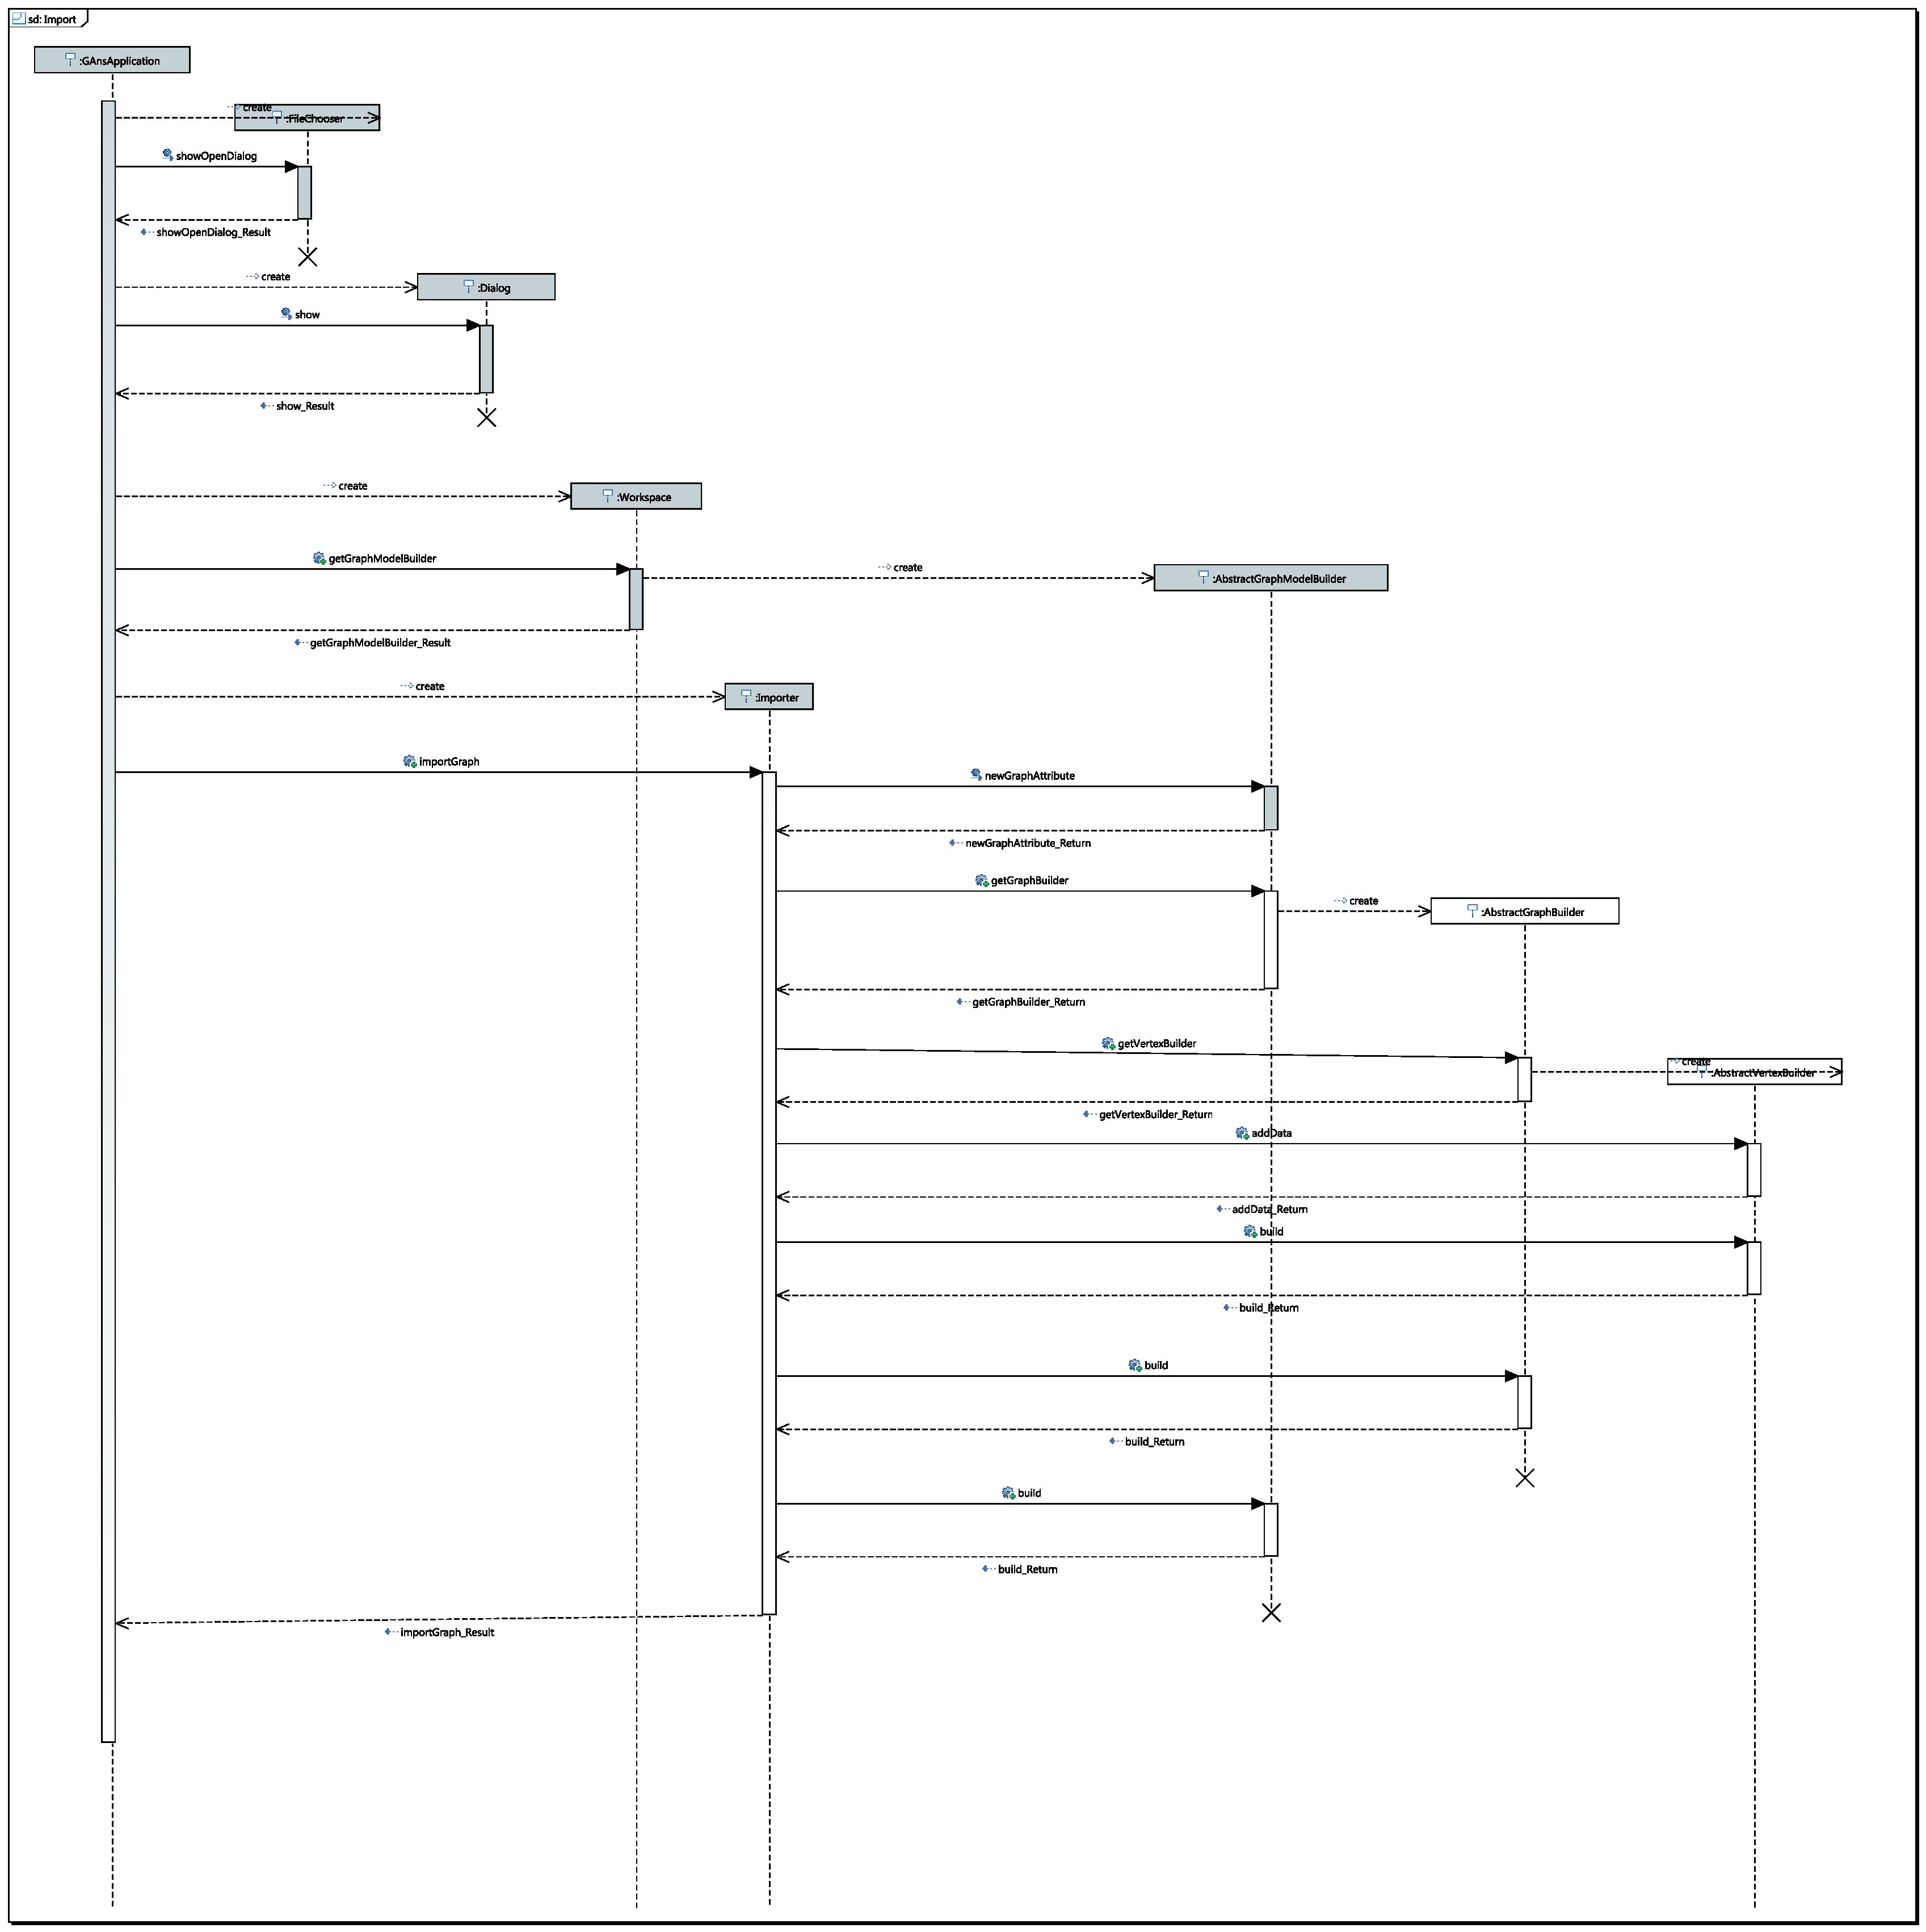
\includegraphics[width=450pt]{resourcen/SeqDiagramImport.PDF}
  \caption{Sequenz Diagramm für den Import}
  \label{fig:seq:import}
\end{figure}

Der Benutzer möchte einen Graphen importieren und klickt auf Import. Die GAnsApplication öffnet einen FileChooser, in welchem der Benutzer die Datei auswählen kann welche er importieren möchte. Danach öffnet sich ein Workspace Dialog in welchem der Benutzer auswählt als welcher Typ der Graph interpretiert werden soll.\\
Das Workspace übergibt der GAnsApplication nun den dazugehörigen IGraphModelBuilder. Dieser wird dann dem Importer übergeben, welcher mithilfe des Builders eine Repräsentation des Graphen erstellt, welche Workspace spezifisch ist.

\newpage

\section{Öffnen eines Graphen über die Strukturansicht}

\begin{figure}[!htbp]
	\centering
	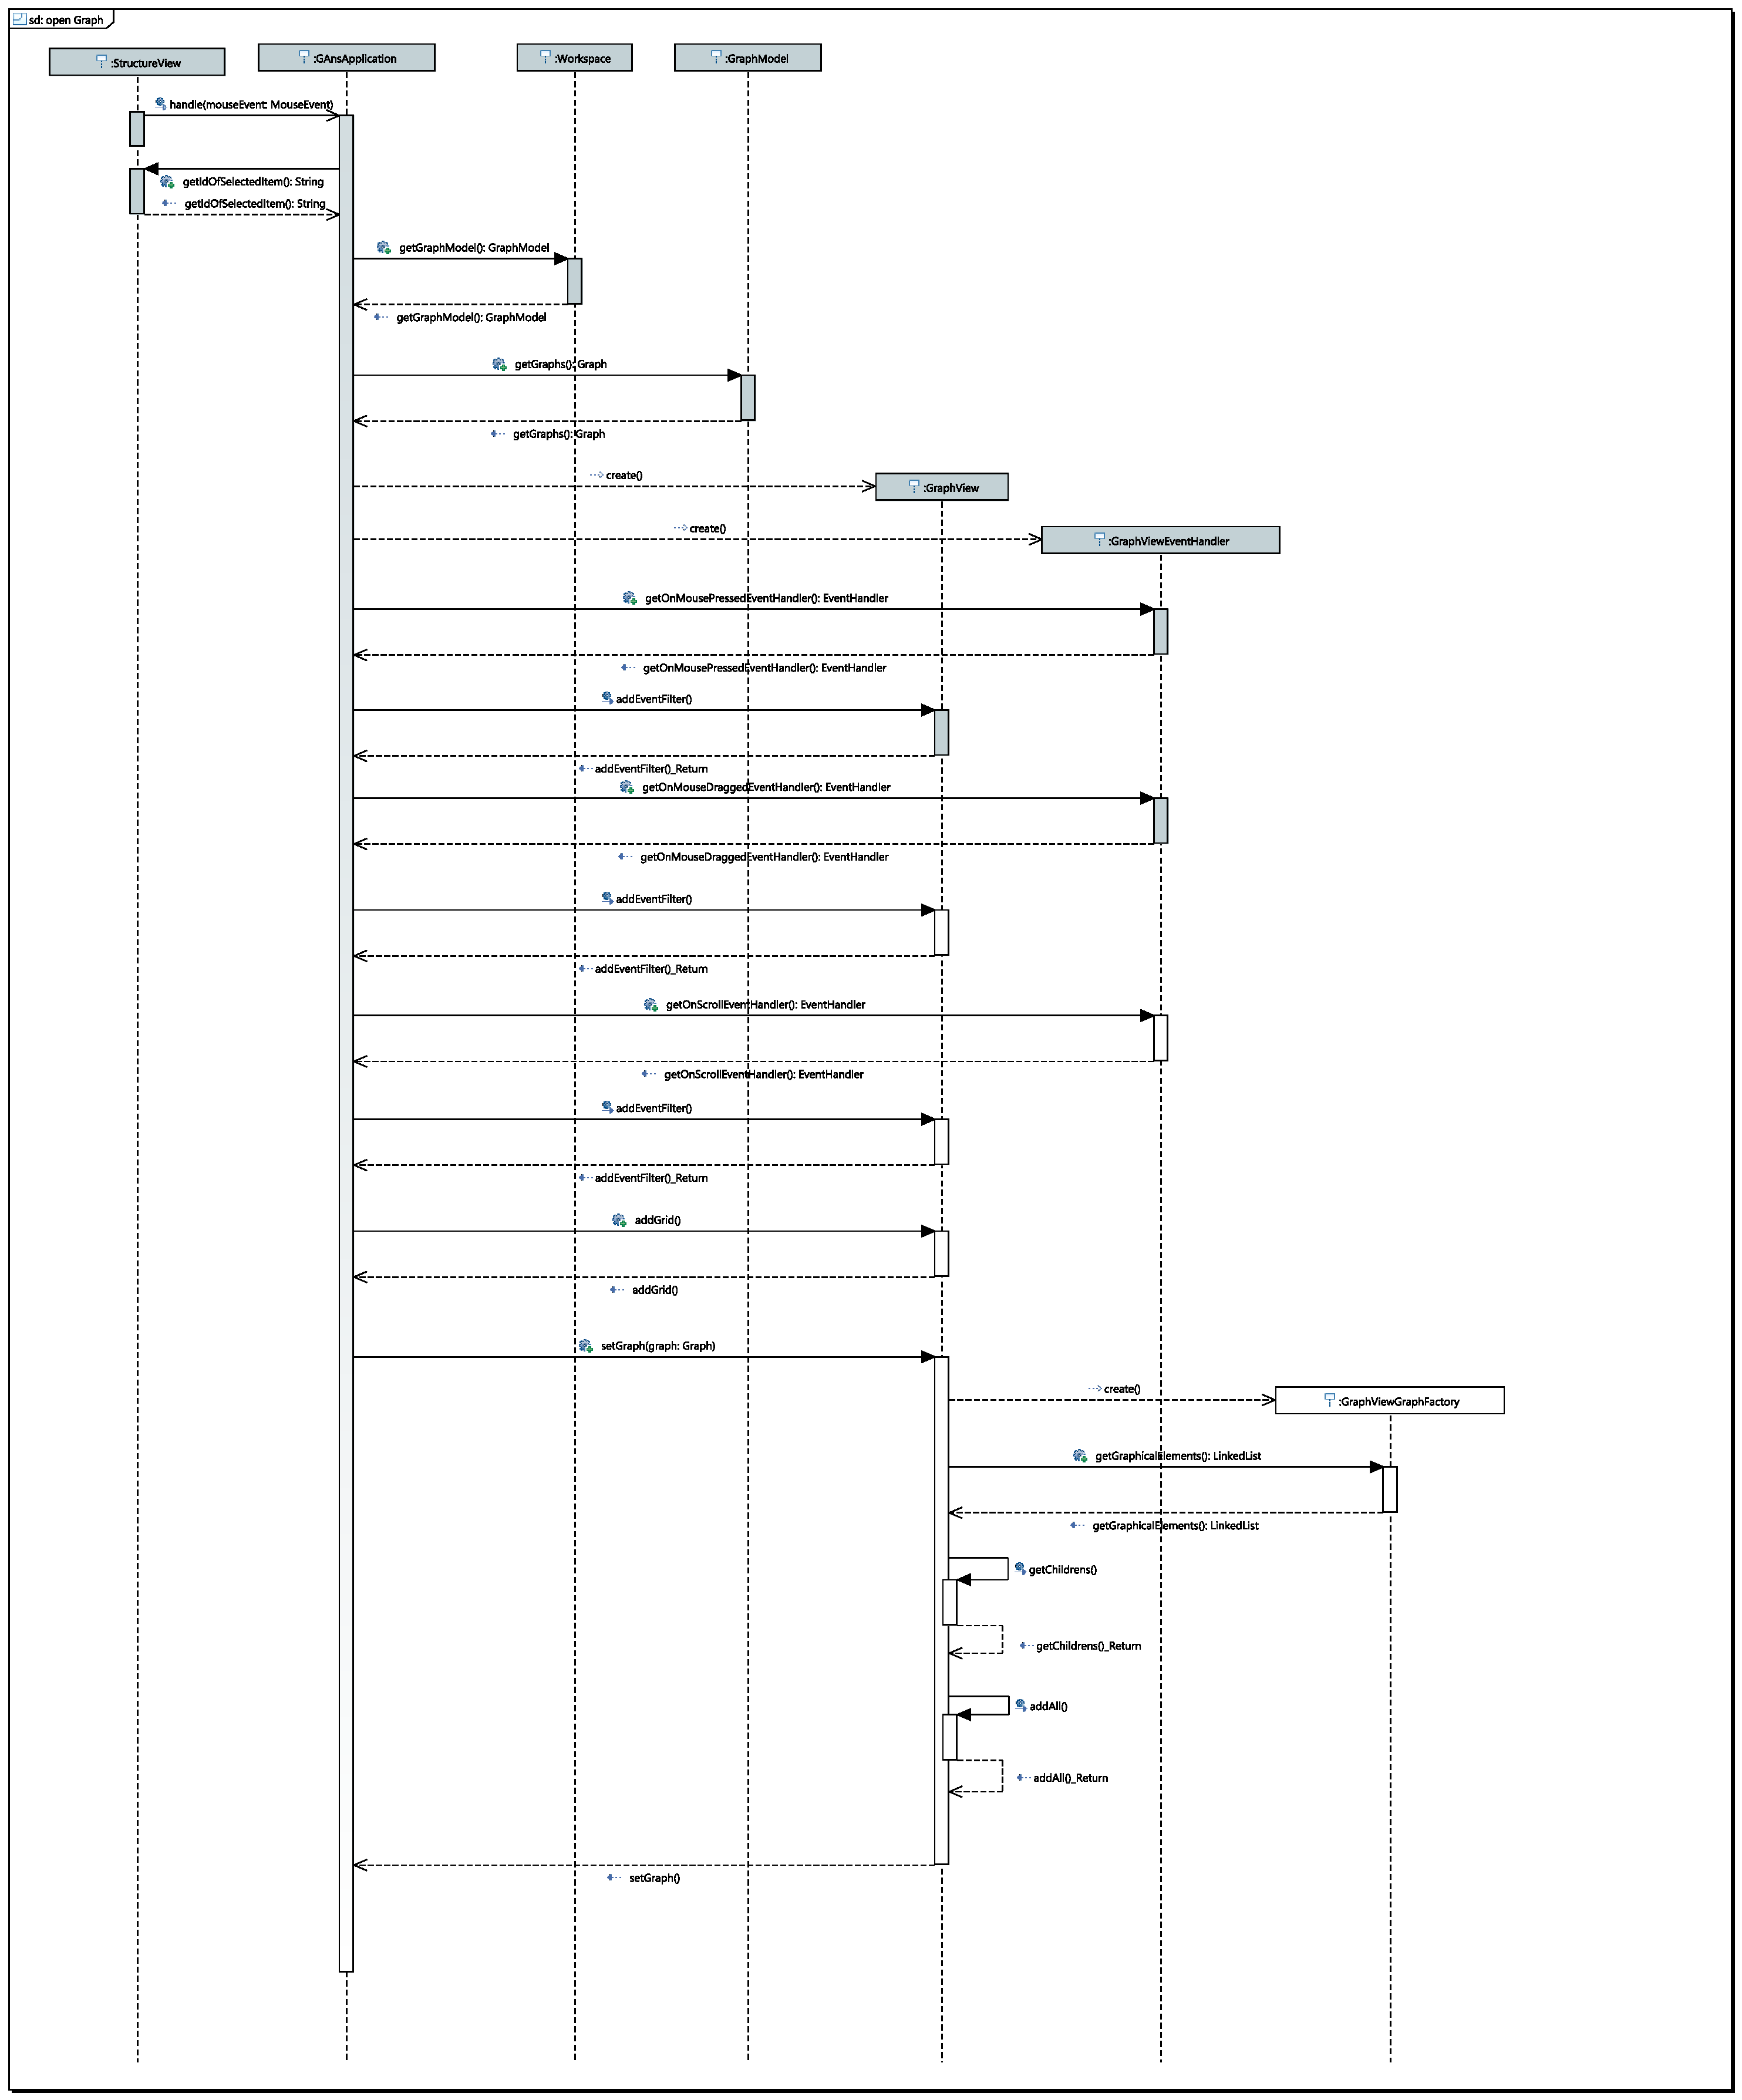
\includegraphics[width=450pt]{resourcen/SeqDiagramOpenGraph.PDF}
	\caption{Sequenz Diagramm das Öffnen eines Graphen aus der Strukturansicht}
	\label{fig:seq:openMethod}
\end{figure}

Der Benutzer hat einen Doppelklick auf ein Element in der StruktureView gemacht. Aus der StruktureView wird die ID des selektierten, gerade doppelt angeklickten, Elements gespeichert. Über das Workspace wird in den Graphen des geladenen GraphModels nach dem zur ID gehörenden Graph gesucht. Der gefundene Graph wird nun gelayouted (siehe \ref{fig:seq:layout}) dabei werden nicht die Dialoge geöffnet, sondern direkt die default LayoutOption des Workspace für den Graphen verwendet. Nachdem der Graph vom layouten zurückgegeben wird, wird eine neue GraphView und ein neues GraphViewEventHandler-Objekt erzeugt, die einzelnen EventFilter werden zur GraphView hinzugefügt und ein Grid wird gesetzt, welches für die Zoom-Funktion benötigt wird. Ist die GraphView aufgesetzt, wird der Graph an sie übergeben. Die GraphView erzeugt eine eigene Factory, welche passend zum Graphen, GraphischeElemente erzeugt. Die GraphView setzt diese Elemente, wodurch sie angezeigt werden.

\newpage

\section{Ändern der Selektion im Graphen}

\begin{figure}[!htbp]
	\centering
	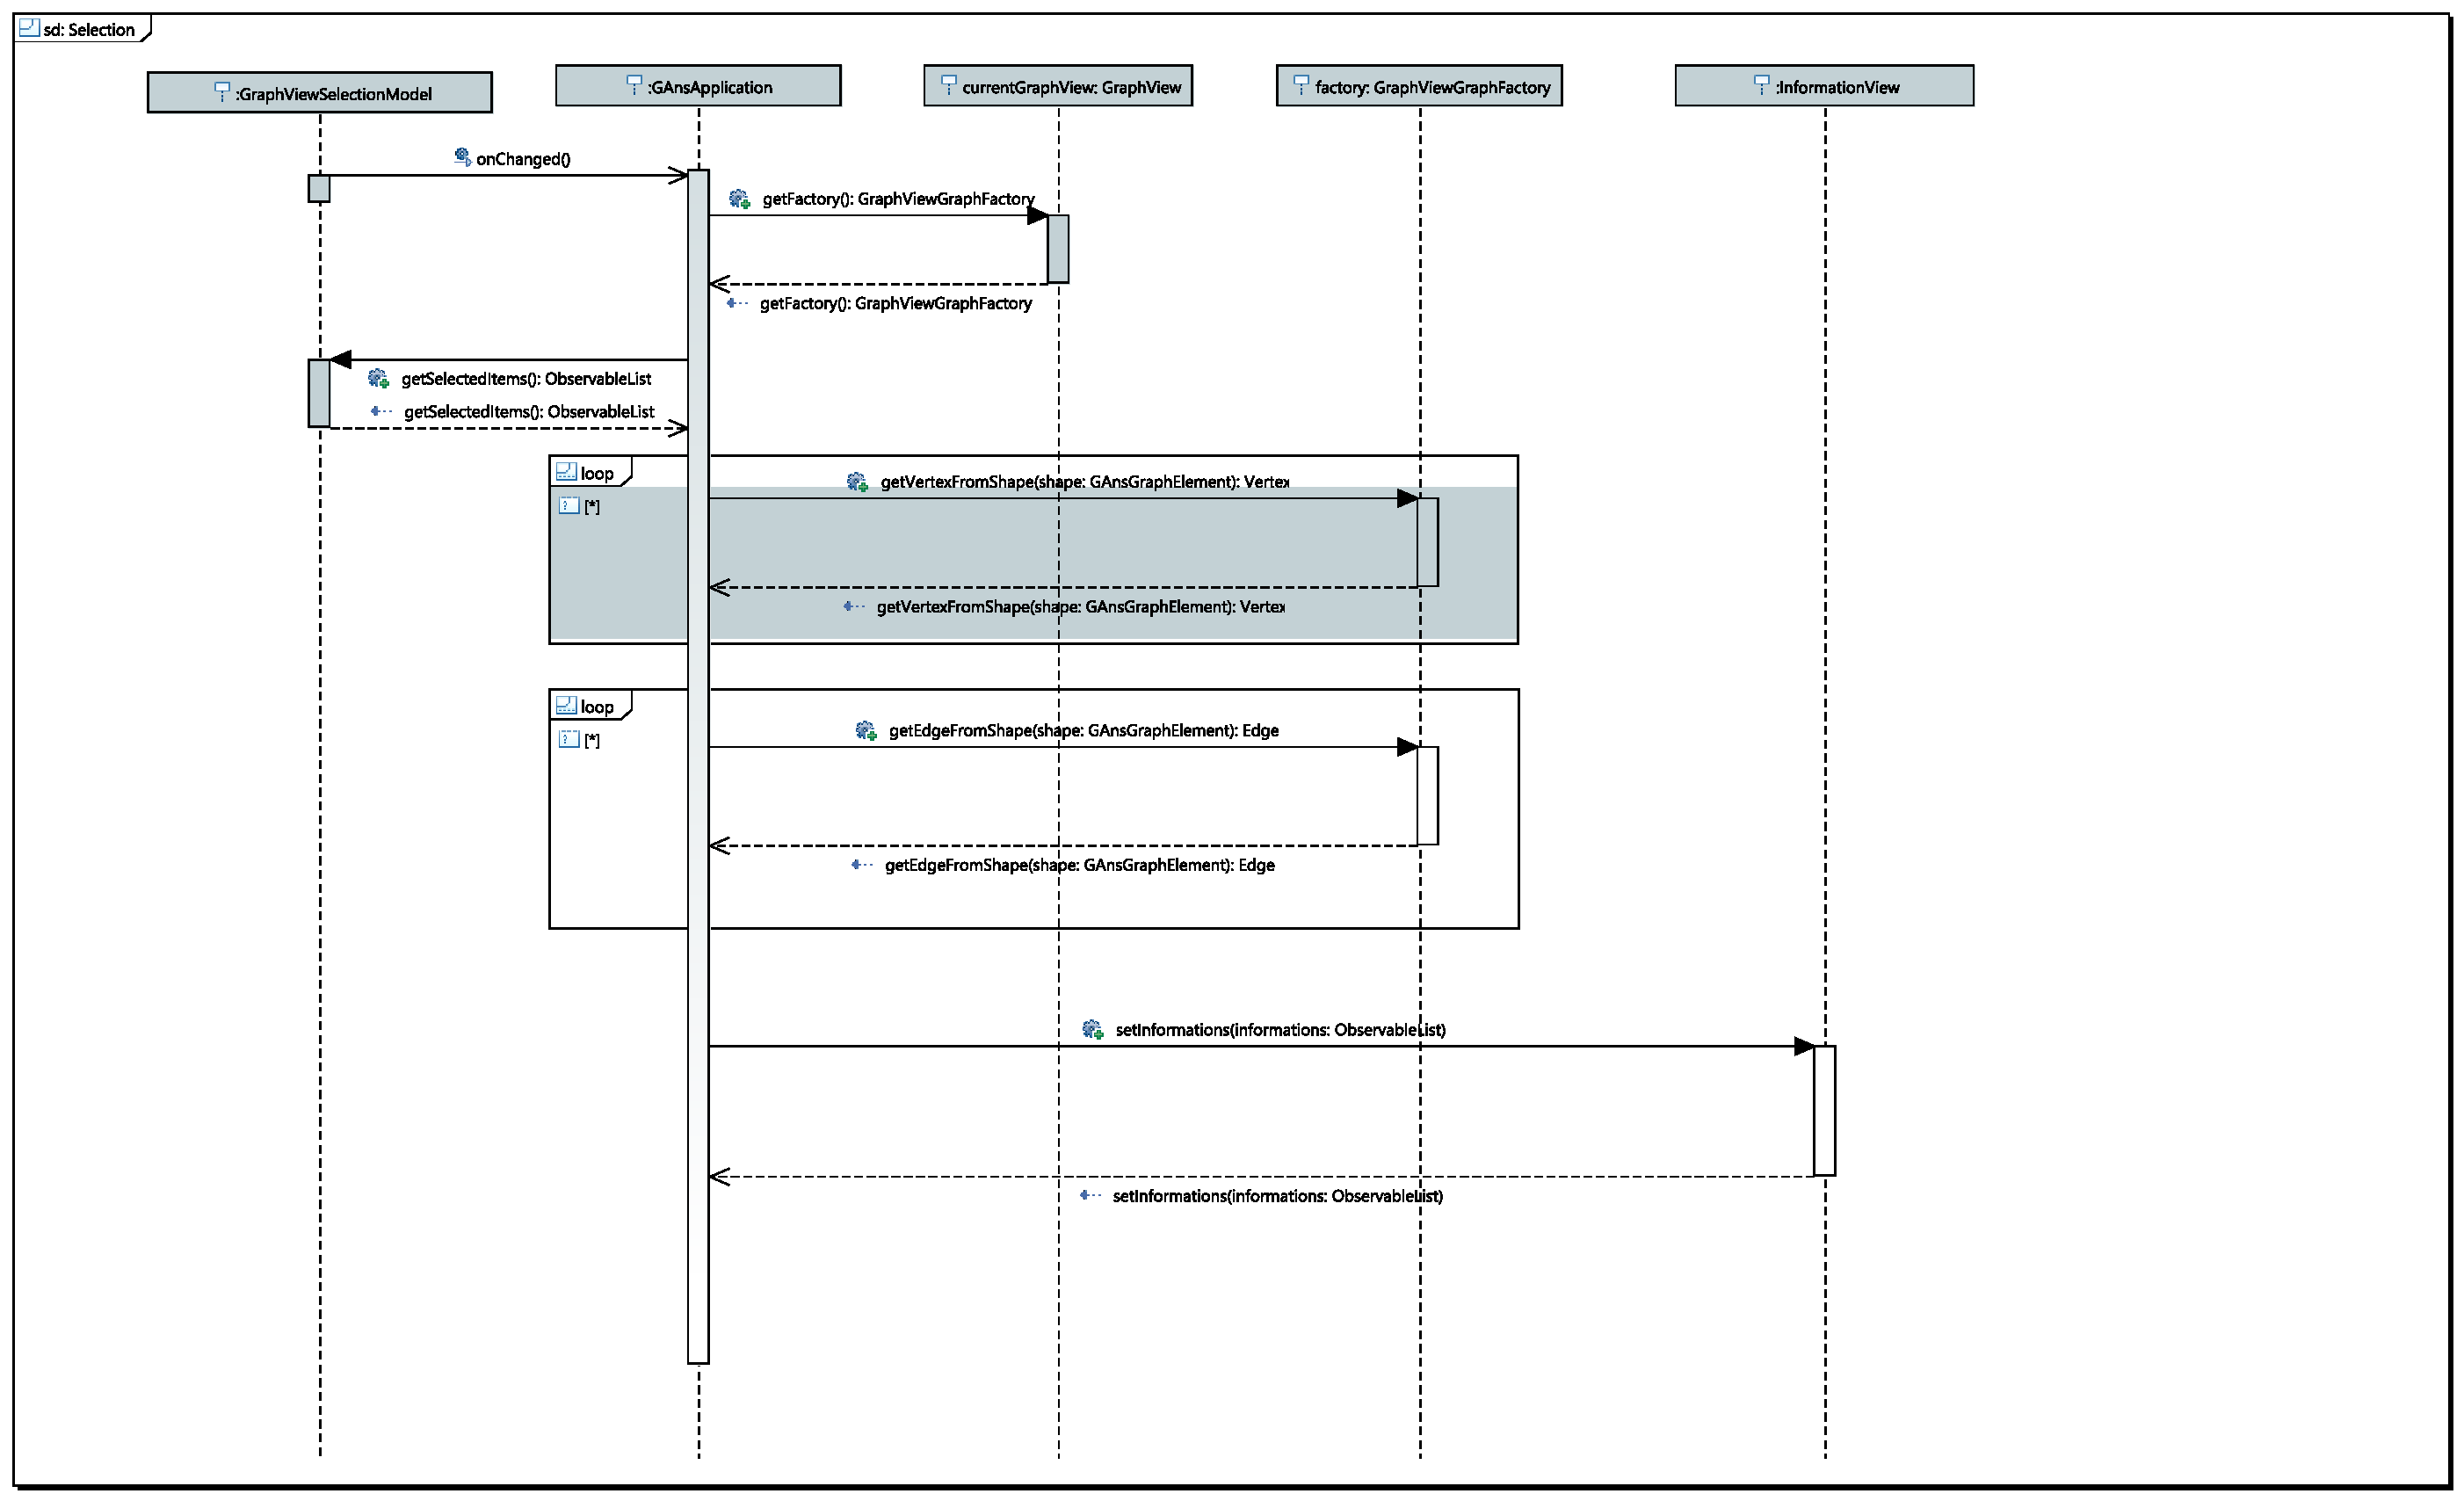
\includegraphics[width=450pt]{resourcen/SeqDiagramSelection.PDF}
	\caption{Sequenz Diagramm für geänderte Selektion}
	\label{fig:seq:selection}
\end{figure}

Der Benutzer hat in der aktuellen GraphAnsicht die Selektion geändert. Die GAnsApplication wird vom GraphViewSelectionModel benachrichtigt. Die GAnsApplication holt sich von der aktuellen GraphAnsicht die Factory, welche zugriff auf die Elemente in der GraphView bietet, und vom SelectionModel eine Liste mit allen selektierten Elementen. Über die Factory und wird nun zu jedem selektiertem Element die zugehörige Vertex oder Edge aus dem angezeigten Graphen ermittelt. Deren GAnsProperties werden in eine ObservableList zusammengeführt und an die InformationsView übergeben, welche die Informationen die über die Properties gegeben sind darstellt.

\newpage

\section{Layouten eines JOANA-Graphs}

\begin{figure}[!htbp]
	\centering
	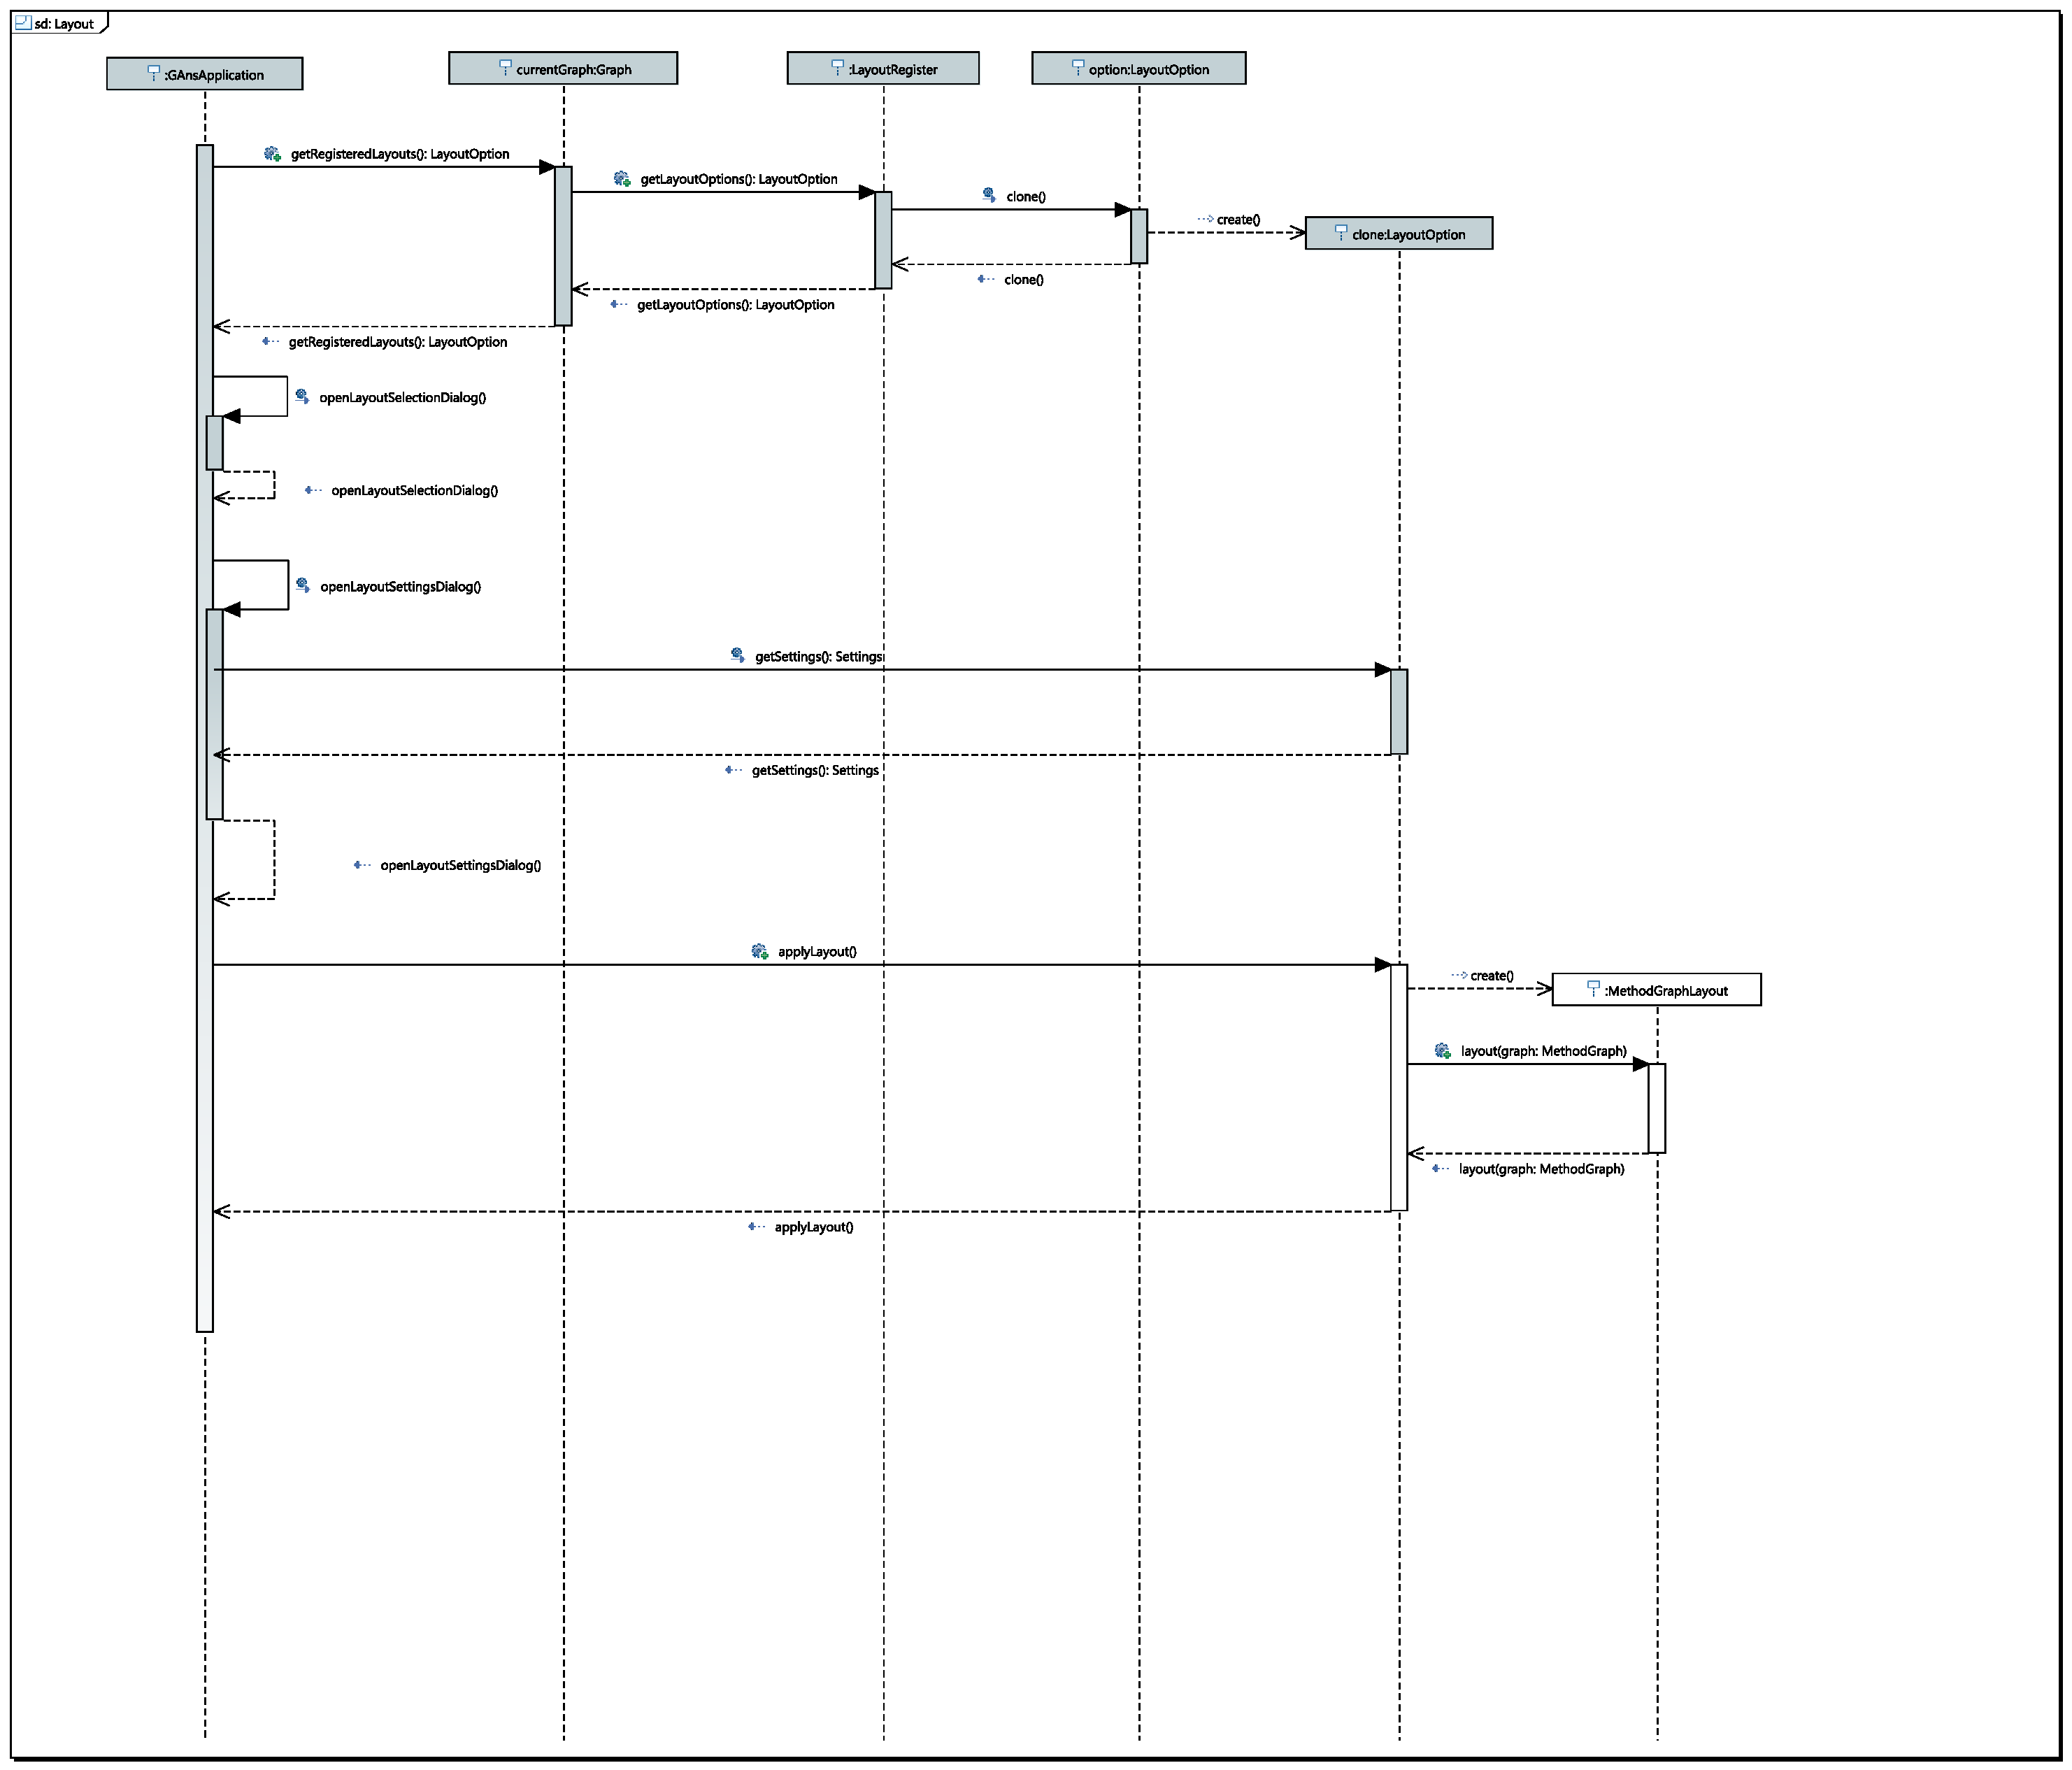
\includegraphics[width=450pt]{resourcen/SeqDiagramLayout.PDF}
	\caption{Sequenz Diagramm für Layouten eines JOANA-Graphs, Oberfläche}
	\label{fig:seq:layout}
\end{figure}

Der Benutzer hat das Layouten des angezeigten Graphen über einen Menüeintrag angestoßen. Die GAnsApplication holt sich über den Graphen alle registrierten LayoutOptions. Diese werden in einem Dialog zur Auswahl gestellt. Nachdem der Benutzer eine Wahl getroffen hat wird ein Dialog geöffnet in dem Einstellungen zur gewählten LayoutOption gemacht werden können. Nun wird auf den gewählten LayoutOption applyLayout aufgerufen, ein MethodGraphLayout erstellt und auf den Graph angewendet(siehe \ref{fig:seq:layoutSugi}).
\newpage

\begin{figure}[!htbp]
	\centering
	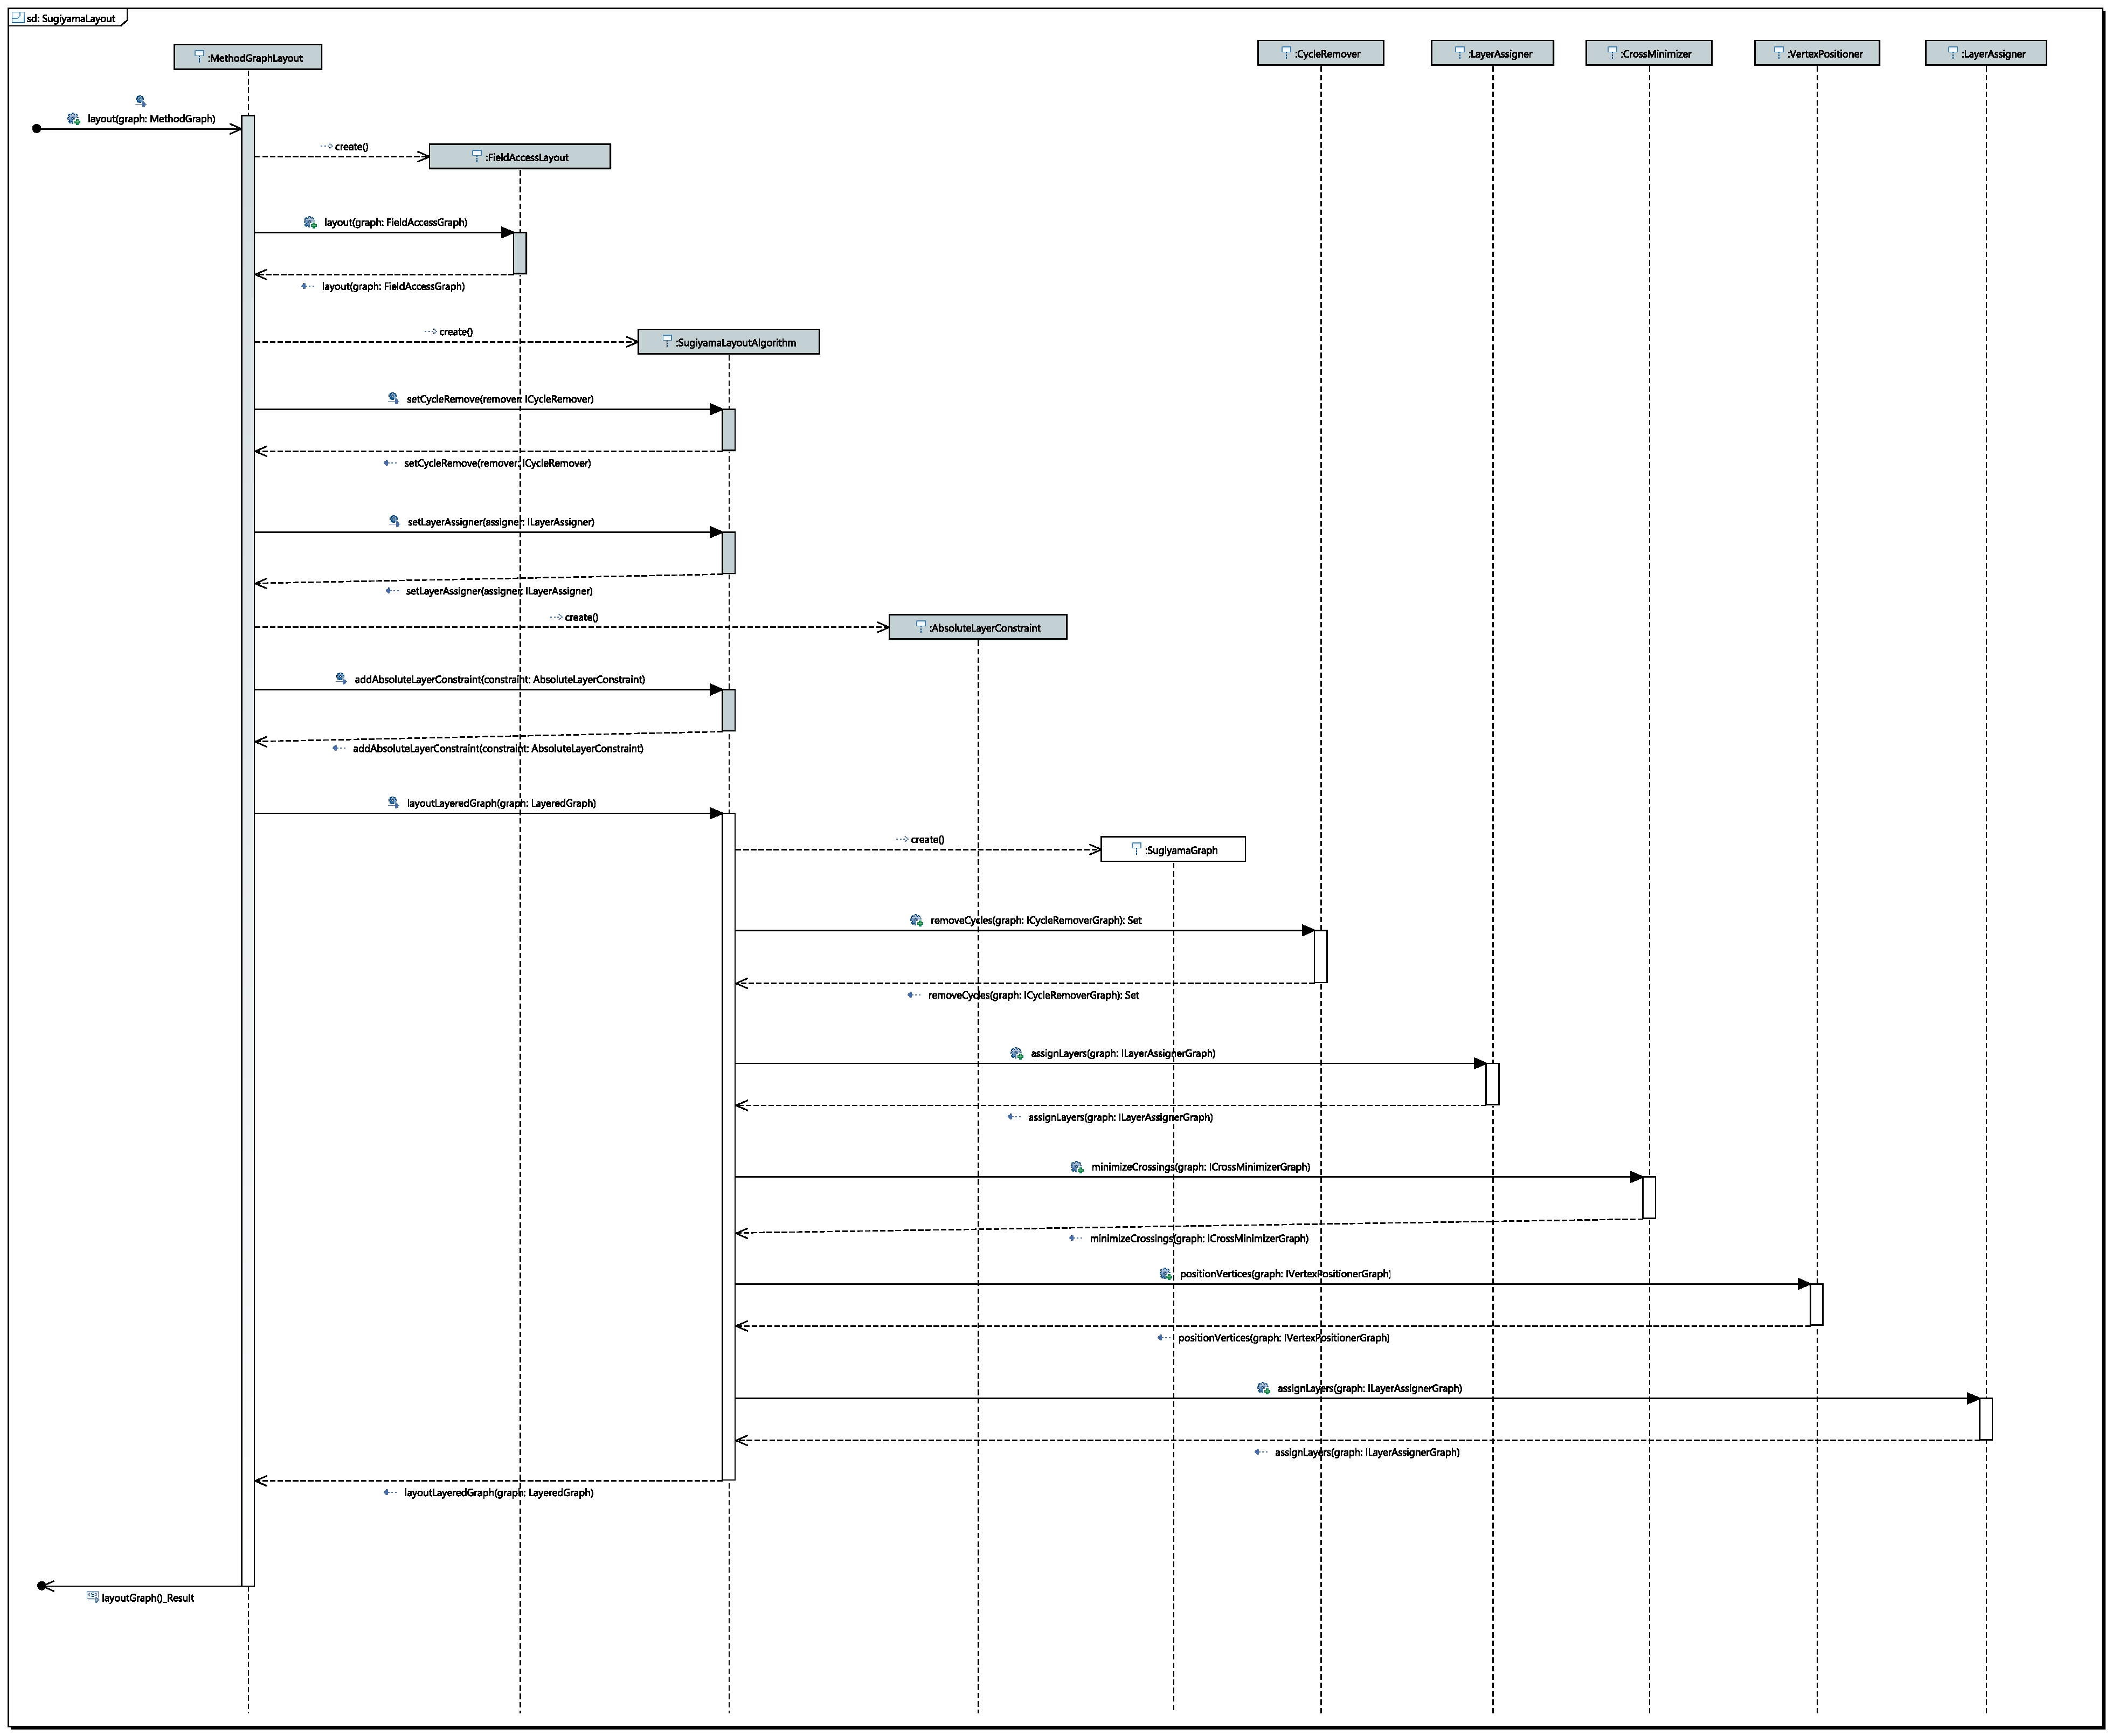
\includegraphics[width=450pt]{resourcen/SeqDiagramSugiyama.PDF}
	\caption{Sequenz Diagramm für Layouten eines JOANA-Graphs, Sugiyama}
	\label{fig:seq:layoutSugi}
\end{figure}

Nachdem das Layouten mit dem MethodGraphLayout angestoßen wurde, wird zuerst ein FieldAccessLayout erstellt und damit alle FieldAccessGraphen des MethodenGraphen gelayouted. Danach wird ein SugiymaLayoutAlgorithm erstellt, die jeweiligen Phasen gesetzt, ein SugiyamaGraph erstellt und die jeweiligen Phasen auf den Graphen angewandt.

\newpage
\section{Export von einem geladenen JOANA-Graphen als SVG}

\begin{figure}[!htbp]
	\centering
	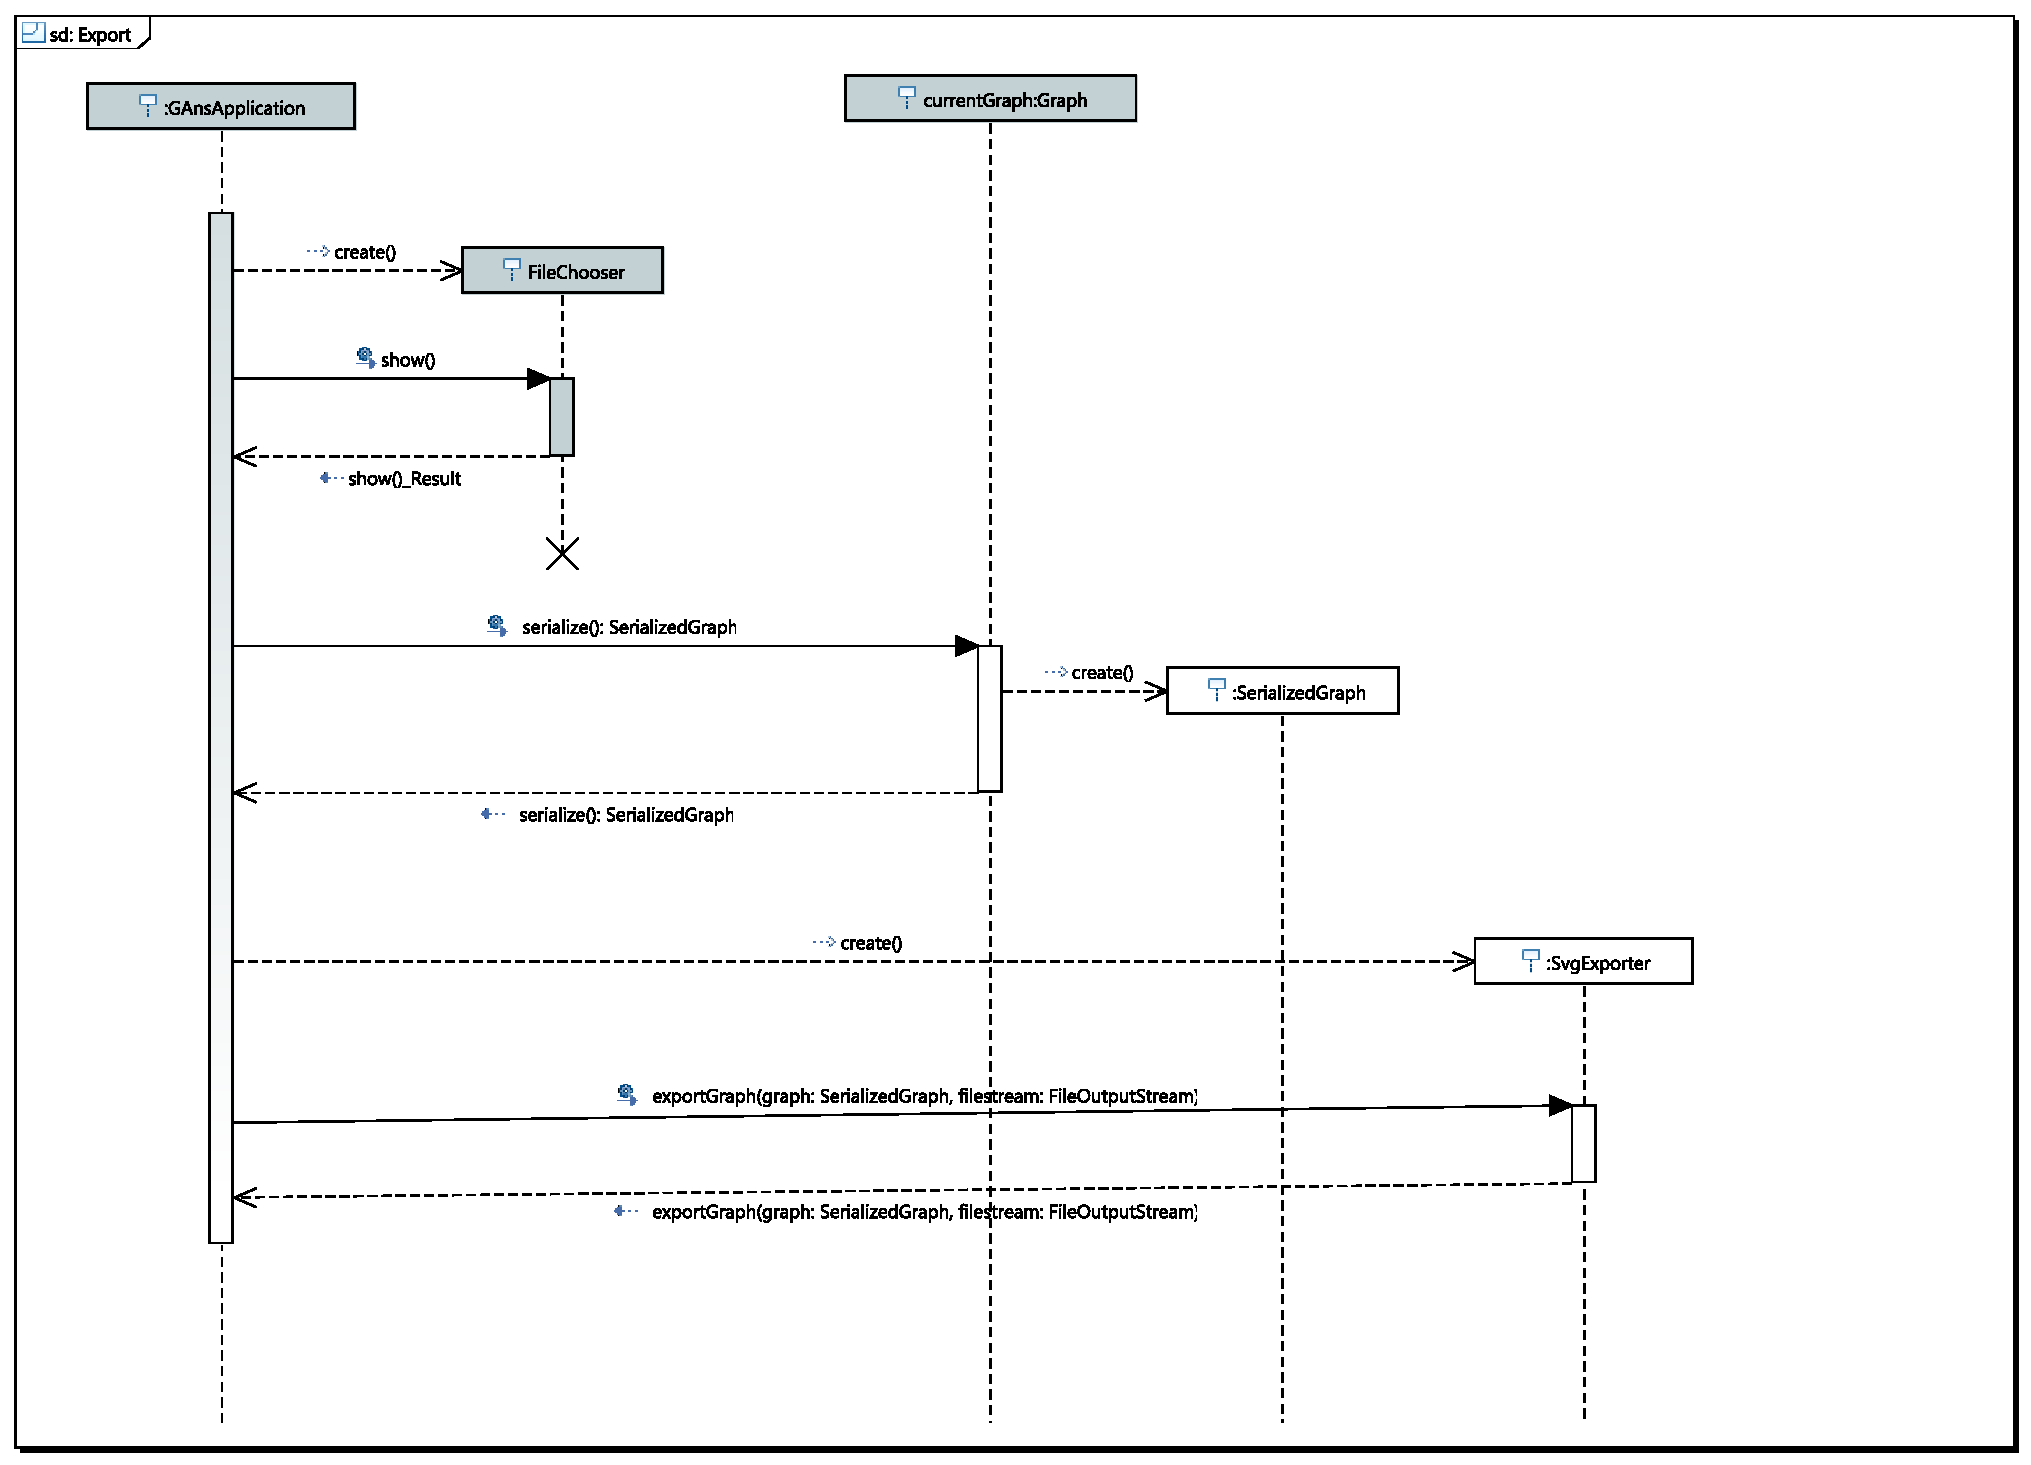
\includegraphics[width=450pt]{resourcen/SeqDiagramExport.PDF}
	\caption{Sequenz Diagramm für Layouten eines JOANA-Graphs, Sugiyama}
	\label{fig:seq:export}
\end{figure}

Der Benutzer möchte einen Graphen exportierten und klickt auf Export. Die GAnsApplication öffnet einen FileChooser, in welchem der Benutzer den Ort und Namen der Datei angeben kann, in die exportiert werden soll. Danach wird der Graph serialisiert und dessen serialisierte Repräsentation in den SvgExporter gegeben, welcher die Daten aus dem Graph in SVG-Form an den ausgewählten Ort schreibt.

\chapter{Paketeinteilung}
\label{ch:paketeinteilung}

Die Paketeinteilung der Software gliedert sich in folgende Pakete: %TODO Paketübersicht

\section{graphmodel}

\begin{figure}[hb]
  \centering
  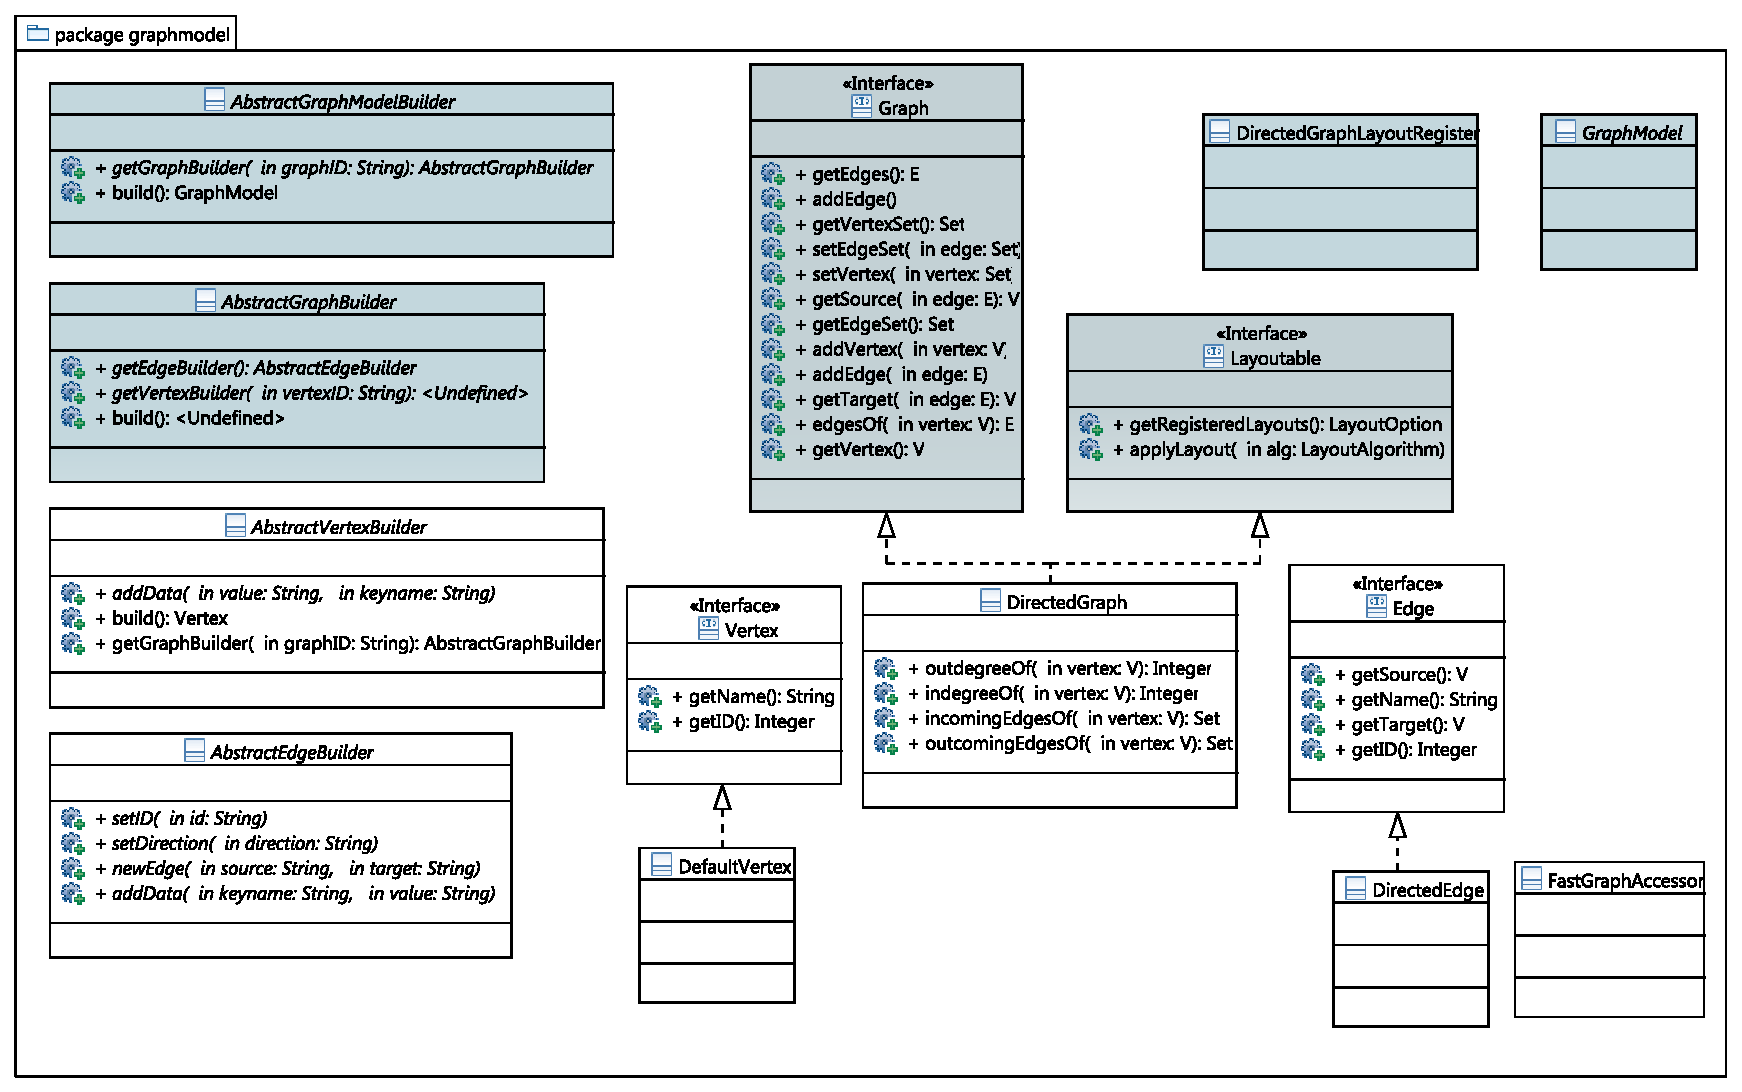
\includegraphics[width=380pt]{resourcen/graphmodel.pdf}
  \caption{Paketübersicht graphmodel}
  \label{fig:packge_graphmodel}
\end{figure}

In dem Paket \textbf{graphmodel} befinden sich die Klassen, die für die interne Repräsentation des Graphen benötigt werden. Die Funktionalität dieses Pakets ist es ein flexibles Graph-Modell, sowie schnellen Zugriff auf dessen Komponenten bereitzustellen.\\ 
Zum Graph-Modell gehören Interfaces wie \textbf{GraphModel}, \textbf{Graph}, \textbf{Vertex} und \textbf{Edge}, welche den groben Aufbau eines Graphen und dessen Funktionalitäten vorgeben. Das \textbf{GraphModel} enthält alle Graphen, welche bei einem Import aus der Datei ausgelesen wurden. Da es Kanten und somit auch Graphen gibt, welche gerichtet sind, gibt es dazu auch passende Interfaces, welche die zuvor genannten erweitern. Zusätzlich gibt es noch weitere Spezialisierungen der Interfaces, wie \textbf{CompoundVertex}, ein Knoten der einen Subgraphen enthält und \textbf{LayeredGraph}, ein Graph der noch Schichten speichert.\\
Die genannten Interfaces sind teilweise schon implementiert. Zu diesen Klassen gehören die \textbf{Default}-Klassen, welche die im Interface definierten Methoden primitiv implementieren und die \textbf{Serialized}-Klassen, welche ein jeweiliges Element darstellen, welche einheitlich für den Export vorbereitet sind. \\
Damit speziellere Implementierungen von \textbf{Graph}, \textbf{Vertex} oder \textbf{Edge} aus \textbf{Plugins} vom \textbf{Importer} einheitlich erstellt werden können gibt es die \textbf{Builder}-Interfaces. Sie geben eine Schnittstelle vor, über welche die speziellen Graphelemente erstellt werden können, ohne dass der \textbf{Importer} davon in Kenntnis gesetzt werden muss.

\newpage

\section{gui}

\begin{figure}[hb]
  \centering
  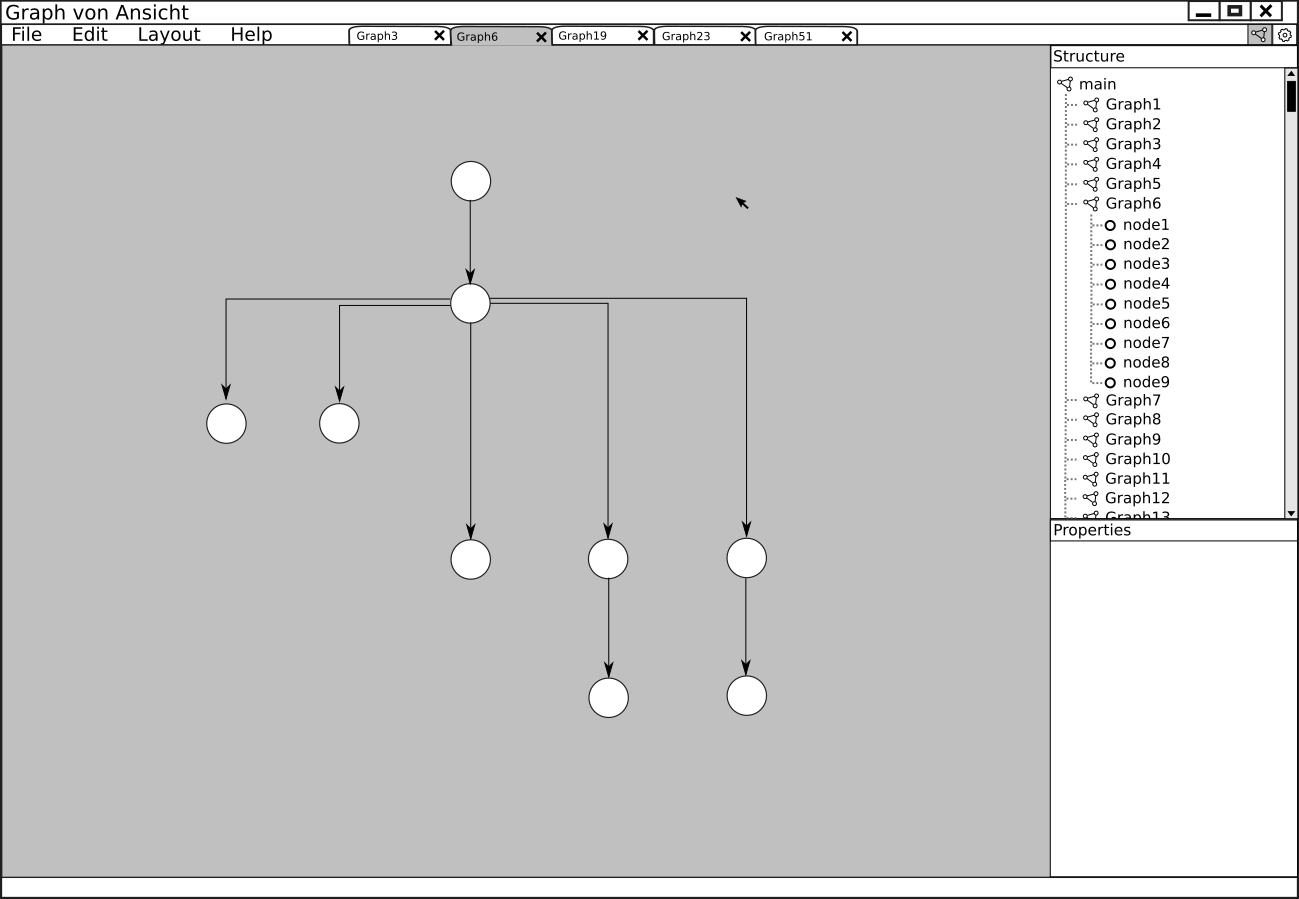
\includegraphics[width=380pt]{resourcen/gui.pdf}
  \caption{Paketübersicht gui}
  \label{fig:packge_gui}
\end{figure}

Das Paket \textbf{gui} beinhaltet die Anzeigelogik, sowie die Haupt-Applikation von GAns. Dafür werden JavaFX Komponenten verwendet, die erweitert und angepasst werden. Es werden Views und Elemente definiert, die für die Anzeige notwendig sind. Die \textbf{GAnsApplication} hat, als Klasse welche das ganze Programm aufsetzt, noch weitere Aufgaben. Sie stößt das Laden der Plugins an und behandelt zusätzlich viele Interaktionen des Benutzers mit den einzelnen GUI-Elementen(siehe SeqDiag Import, doppelklick, selection) unter anderem auch das Laden bzw. Erstellen des unterliegenden GraphModels(siehe graphmodel). Es werden verschiedene Views definiert:
\begin{itemize}[labelindent=0pt,labelwidth=\widthof{\textbf{InformationView}},itemindent=0em,leftmargin=!]
	\item[\textbf{GraphView}] Eine View welche den gelayouteten Graphen anzeigt und dazu verschiedene Navigationsmöglichkeiten, wie Zoom, Selektion usw., anbietet. Es können mehrere GraphViews gleichzeitig geöffnet sein. Jede einzelne ist in einem eigenen Tab enthalten, zwischen denen hin und her gewechselt werden kann. Die Elemente welche in der GraphView angezeigt werden, sind \textbf{GAnsGraphElemente}. Sie bestehen aus verschiedenen JavaFX Klassen, welche einen Text und eine Farbe gesetzt bekommen können. Standardmäßig werden Rechtecke für Knoten und direkte Kanten als Kanten zwischen Knoten verwendet.
	\item[\textbf{StructureView}] Eine TreeView, welche die geschachtelten Graphen einer importierten Datei anzeigt. Über doppelklick auf eines der Baumelemente wird der durch das Element dargestellte Graph in einer neuen GraphView angezeigt. Zum Erstellen der einzelnen Baumelemente werden normale JavaFX-Funktionalitäten verwendet.
	\item[\textbf{InformationView}] Eine TableView, welche, je nach Selektion in der aktuell angezeigten GraphView, Informationen über die selektierten Elemente anzeigt. Jede Zeile der Tabelle enthält in der ersten Zelle den Bezeichner/Namen und in der zweiten Zelle den jeweiligen Wert der Eigenschaft aus der Selektion. Die einzelnen Zellen werden durch eine JavaFX \textbf{PropertyValueFactory} erstellt welche mit den \textbf{GAnsProperties}(siehe objectproperty) der selektierten Elemente der GraphView arbeitet. 
\end{itemize}

\newpage

\section{parameter}

\begin{figure}[hb]
  \centering
  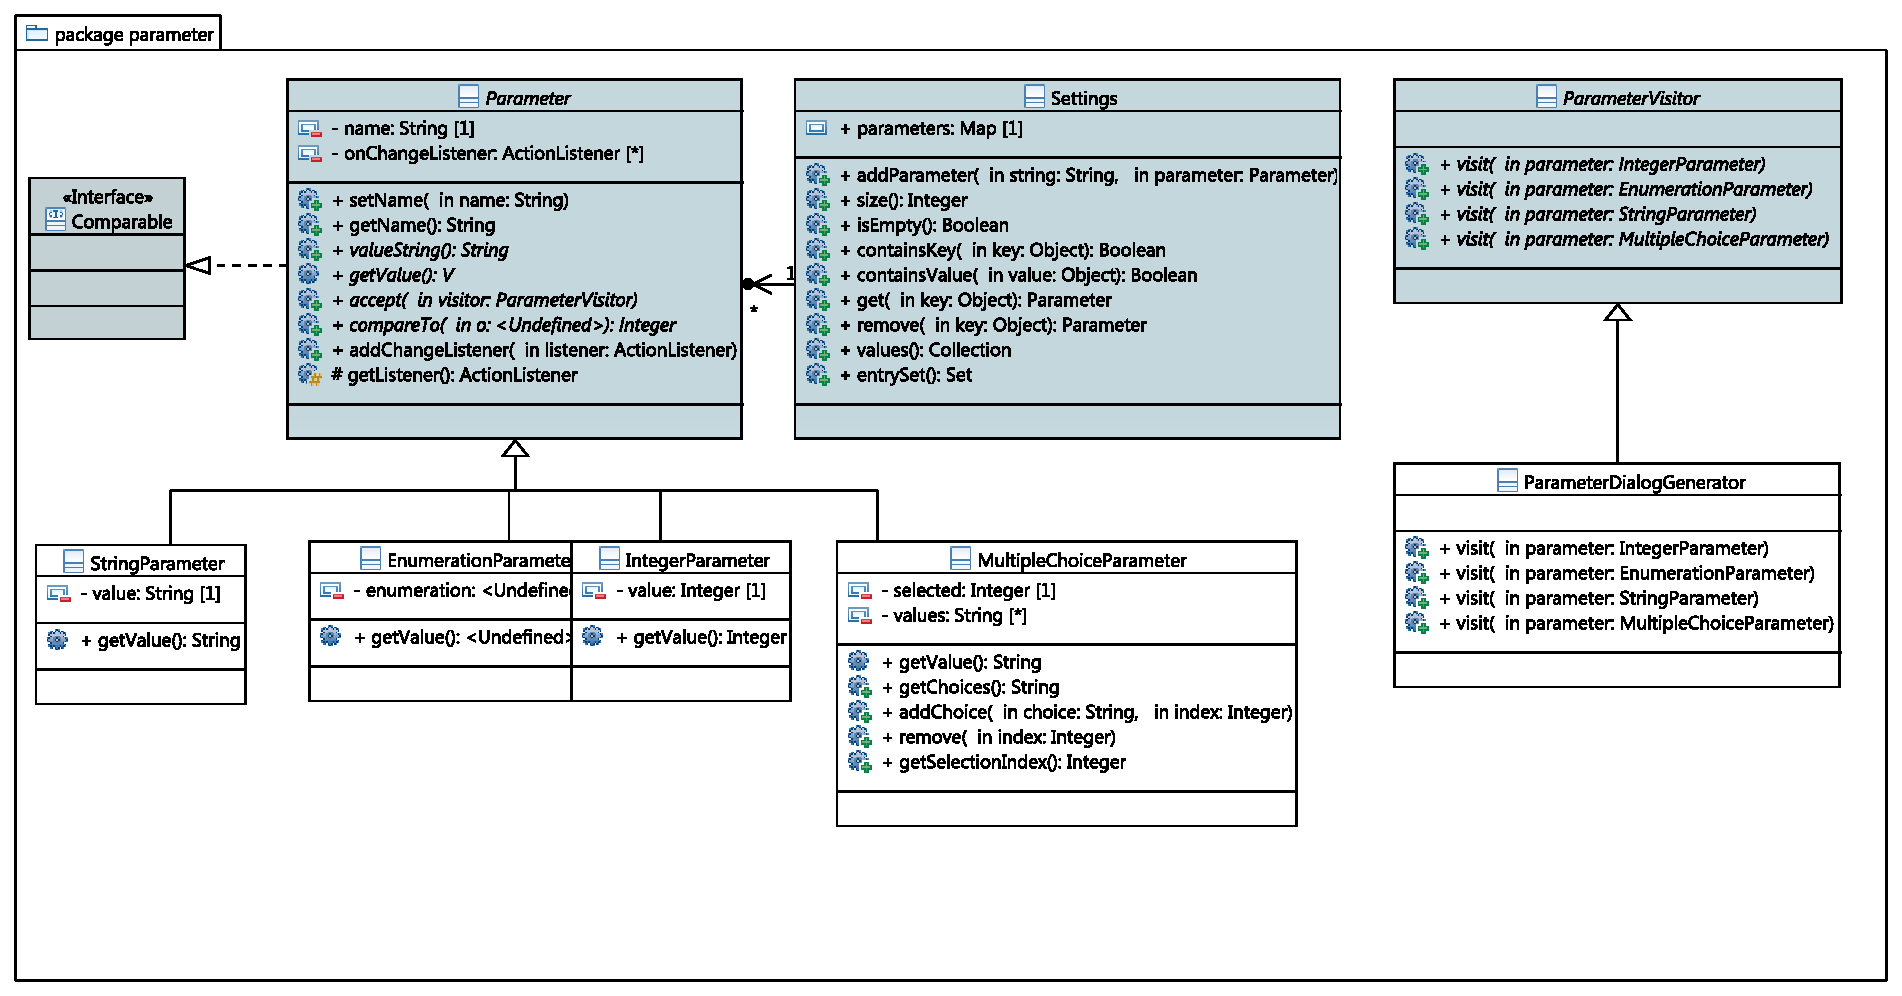
\includegraphics[width=380pt]{resourcen/parameter.pdf}
  \caption{Paketübersicht parameter}
  \label{fig:packge_parameter}
\end{figure}

Dieses Paket trennt Rahmenbedingungen(Parameter) von Layouts oder Constraints in eigene Klassen. Diese Wrapper-Klassen erlauben z.B. einem Layout seine Einstellungsmöglichkeiten an die GUI zu übergeben, ohne das vom Layout aus Wissen über GUI-Elemente gefordert wird. \\Die implementierten Parameter können von Visitors besucht werden, welche den Wert des Parameters auslesen und verändern können. Im GUI-Paket gibt es eine Generator-Klasse, welche einen solchen Visitor implementiert. Somit können die Einstellungsdialoge automatisch gefüllt werden und gemachte Änderungen im Dialog werden direkt wieder in den Parametern gesetzt. Da in gewissen Situationen von der GUI, oder dem zugehörigen Layout, Listener auf die Werte gesetzt werden müssen, erben die Parameter von GAnsProperty, da diese bereits viel benötigte Funktionalität vereinfacht anbieten und Gemeinsamkeiten aufweisen.

\newpage

\section{graphRegex}

\begin{figure}[hb]
  \centering
  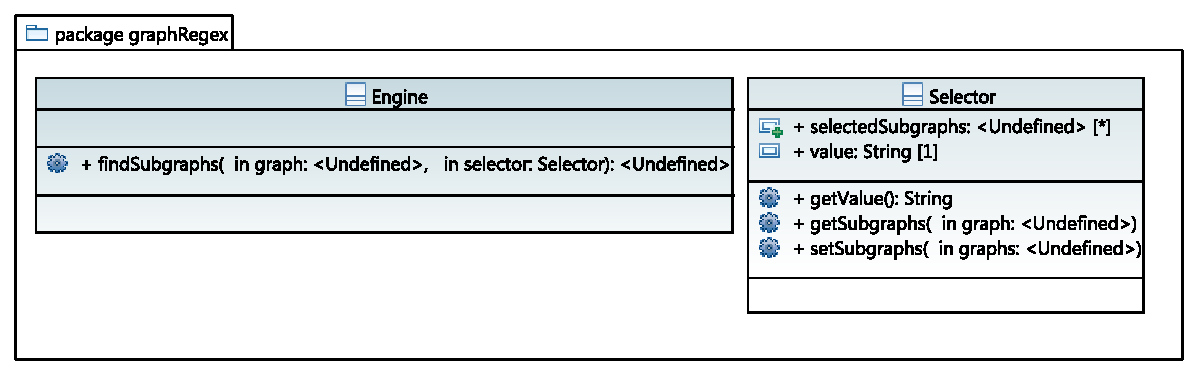
\includegraphics[width=380pt]{resourcen/graphRegex.pdf}
  \caption{Paketübersicht graphRegex}
  \label{fig:packge_graphRegex}
\end{figure}

In diesem Paket befinden sich die Algorithmen zum durchsuchen von Graphen nach Subgraphen mithilfe von Selektoren. Es gibt eine \textbf{Selector} Klasse, welche die Information, welche Subgraphen selektiert werden sollen, speichert und eine \textbf{Engine}, die aus einem gegebenen Graphen die Subgraphen, welche die Beschreibung erfüllen, heraussucht und zurückgibt. Dieses Paket dient hauptsächlich als Helfer für Layoutalgorithmen, die auf diese Weise für gegebene Constraints bestimmte Subgraphen selektieren und speziell verarbeiten können.

\newpage

\section{objectproperty}

\begin{figure}[hb]
  \centering
  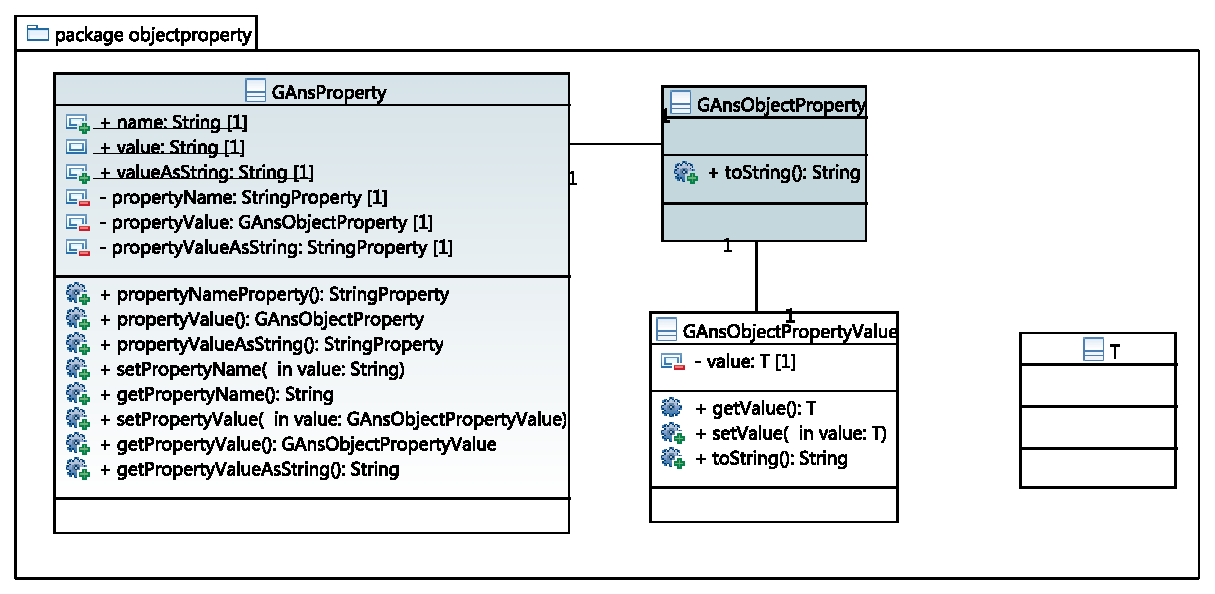
\includegraphics[width=380pt]{resourcen/objectproperty.pdf}
  \caption{Paketübersicht objectproperty}
  \label{fig:packge_objectproperty}
\end{figure}

Das Paket \textbf{objectproperty} bietet eine generische Eigenschaft eines Elements aus dem Paket \textbf{graphmodel}. Dabei stellt jede \textbf{GAnsProperty} eine einzelne Eigenschaft dar, welche aus einen Bezeichner/Namen, einen generischen Wert und eine Stringrepräsentation des Werts besteht. Die einzelnen Bestandteile werden in JavaFX ObjectProperties gespeichert. Darunter die \textbf{GAnsObjectProperty}, welche einen generischen Typ unterstützt. Diese Properties harmonieren gut mit den restlichen JavaFX-GUI-Elementen, somit kann auf viele Funktionen zurückgegriffen werden kann die von JavaFX direkt angeboten werden ohne große Eigenentwicklungen anfertigen zu müssen. Das beste Beispiel dafür ist die InformationView der GUI, deren Inhalt durch \textbf{PropertyValueFactories} von JavaFX automatisch erstellt werden, sobald eine Liste mit GAnsProperties gesetzt wird. Dabei ist der eigentliche Typ des Werts irrelevant, da in der GUI auf die Stringrepräsentation des Werts zugegriffen werden kann, wobei z.B. im Model oder Layoutalgorithmus mit dem eigentlichen Wert gearbeitet werden kann. Die PropertyValueFactories arbeiten mit dem Bestandteil der GAnsProperty, welcher mit einem bestimmten Referenz-String erstellt wurde. Diese Strings sind in GAnsProperty statisch gegeben, sodass die Aufrufe selbst bei Änderungen in der GAnsProperty im restlichen Programm konstant bleiben.

\newpage

\section{plugin}

\begin{figure}[hb]
  \centering
  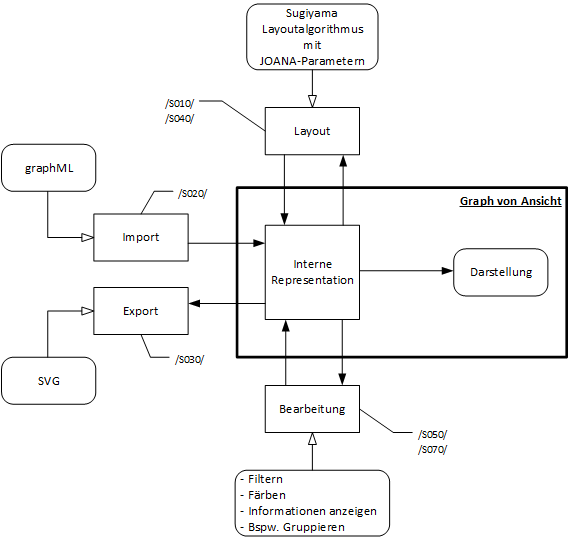
\includegraphics[width=380pt]{resourcen/plugin.pdf}
  \caption{Paketübersicht plugin}
  \label{fig:packge_plugin}
\end{figure}

Das Paket \textbf{plugin} bietet Interfaces für Plugins sowie einen \textbf{PluginManager} welcher die Plugins lädt, verwaltet und zur Verfügung stellt. Klassen die Interfaces dieses Plugins implementieren müssen sich beim laden, der Klasse die \textbf{Plugin} erweitert beim \textbf{PluginManager} registriert werden, um dann vom Programm verwendet werden zu können. Es bietet somit die Möglichkeit Funktionalität von außen zu laden und somit das Programm zu erweitern. \\
Ein \textbf{Importer} und ein \textbf{Exporter} Interface können implementiert werden um weitere File Importer oder Exporter hinzuzufügen. \\
Ein \textbf{LayoutAlgorithm} ist in der Lage einen Graphen zu layouten. Er hat \textbf{LayoutOption}s und \textbf{Constraint}s die eingestellt werden können, um die funktionsweise des Algorithmus zu beeinflussen. Die \textbf{LayoutOption}s können dann in einem \textbf{LayoutRegister} gespeichert werden. \\
\textbf{EdgeFilter}, \textbf{VertexFilter} und \textbf{FilterSet} erlauben es Plugins Filter für Kanten und Knoten zu definieren die bei Layouten und Darstellung unbeachtet bleiben. \\
\textbf{Workspace}s beschreiben eine Arbeitssituation in der spezifische Graphtypen verarbeitet werden können. Ein Beispiel hierfür ist der \textbf{JoanaWorkspace} im \textbf{joana} Paket. Ein Workspace definiert, welche Dateien mit welchem Importer importiert werden und ermöglicht so das öffnen spezifischer Graphtypen welche in generischen Formaten wie graphml gespeichert werden können. Dieses kann wiederum über \textbf{WorkspaceOption}s eingestellt werden.\\

\newpage

\section{sugiyama}

\begin{figure}[hb]
  \centering
  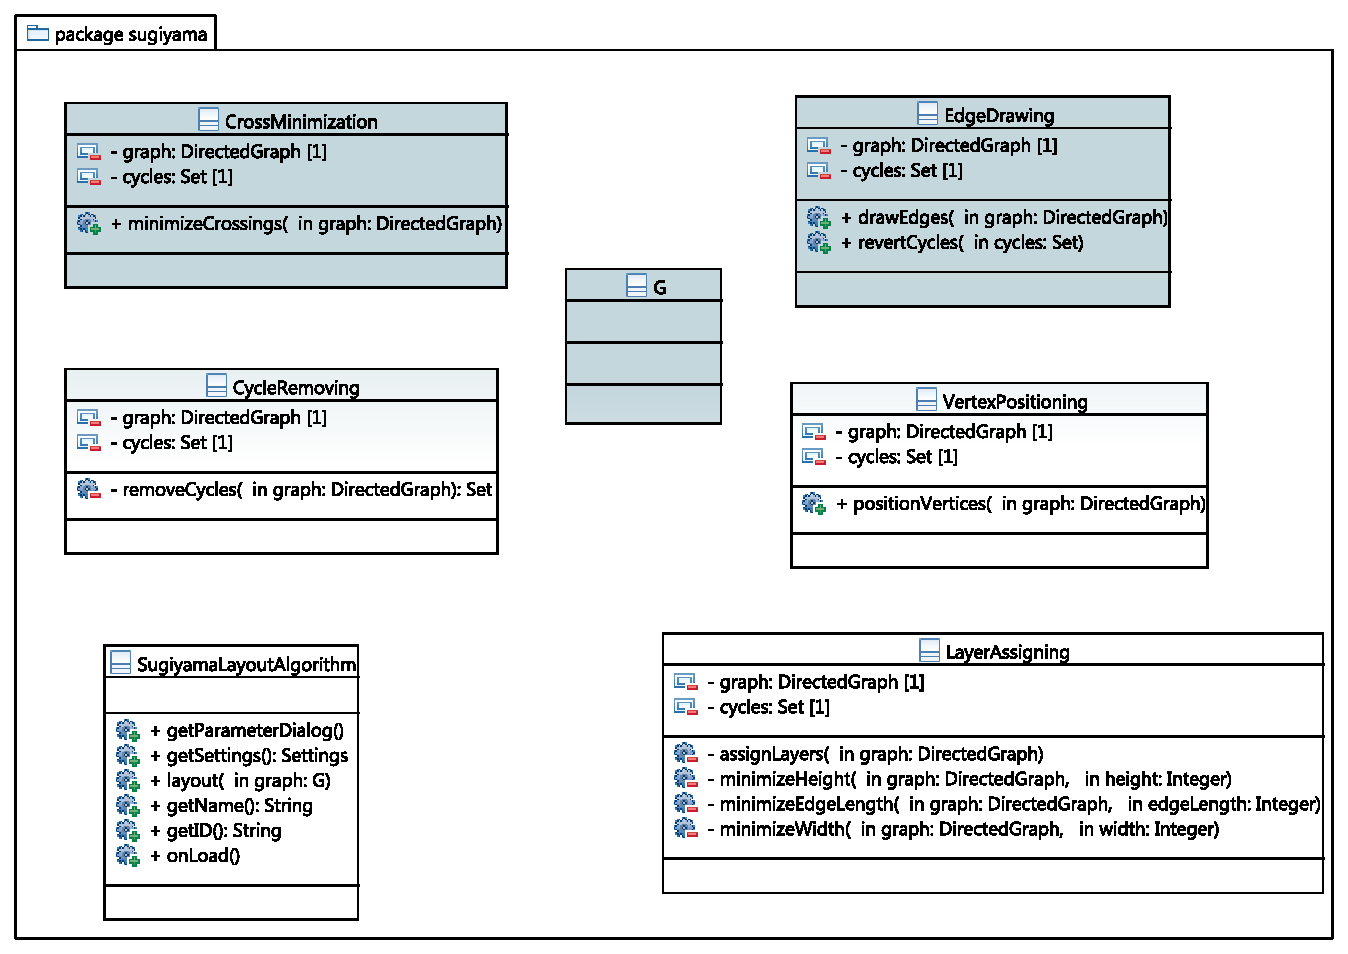
\includegraphics[width=380pt]{resourcen/sugiyama.pdf}
  \caption{Paketübersicht sugiyama}
  \label{fig:packge_sugiyama}
\end{figure}

Das Paket \textbf{sugiyama} bietet neben einer Implementierung des Sugiyama-Frameworks zum hierarchischen layouten eines gerichteten Graphen Schnittstellen zum ändern und austauschen einzelner Phasen dieses Frameworks.\\
Die fünf Phasen des Sugiyama-Frameworks: Kreise entfernen, Lagenzuordnung, Kreuzungsminimierung, Knotenpositionierung und Kantenzeichnen werden in dieser Reihenfolge durchlaufen und durch einen \textbf{SugiyamaLayoutAlgorithm} verwaltet und gesteuert. Die Klassen, die diese Schritte darstellen \textbf{CycleRemover}, \textbf{LayerAssigner}, \textbf{CrossMinimizer}, \textbf{VertexPositioner} und \textbf{EdgeDrawer} arbeiten auf einem \textbf{SugiyamaGraph}, welcher den zu layoutenden Graphen repräsentiert. Hierzu implementiert er die jeweiligen Interfaces, die diese Schritte fordern.\\
In der ersten Phase werden die Zykel des Graphen entfernt, indem die Richtungen einer minimalen Kantenmenge umgekehrt wird.\\
Anschließend wird jedem Knoten eine Lage zugewiesen, welche abhängig von der Anzahl der ein- und ausgehenden Kanten des Knotens, sowie der Länge des kürzesten Pfades des Knotens zu einem Knoten aus der ersten Lage ist. Zudem werden, falls eine Kante zwischen zwei Knoten mindestens eine Lage überspringt, in jede dieser Lagen ein \textbf{DummyVertex} ein.\\
In der dritten Phase wird die Anzahl der Kantenkreuzungen minimiert. Dazu werden jeweils in zwei aneinanderliegenden Lagen die Knoten beider Lagen umgeordnet.\\
In Phase Vier bekommen die Knoten feste Positionen in den Lagen zugewiesen\\
In der letzten Phase wird jeder \textbf{DummyVertex} entfernt und die Kanten werden gezeichnet. Zusätzlich werden die im ersten Schritt umgedrehten Kanten wieder in ihre ursprüngliche Richtung zurückversetzt.

\newpage

\section{joana}

\begin{figure}[hb]
  \centering
  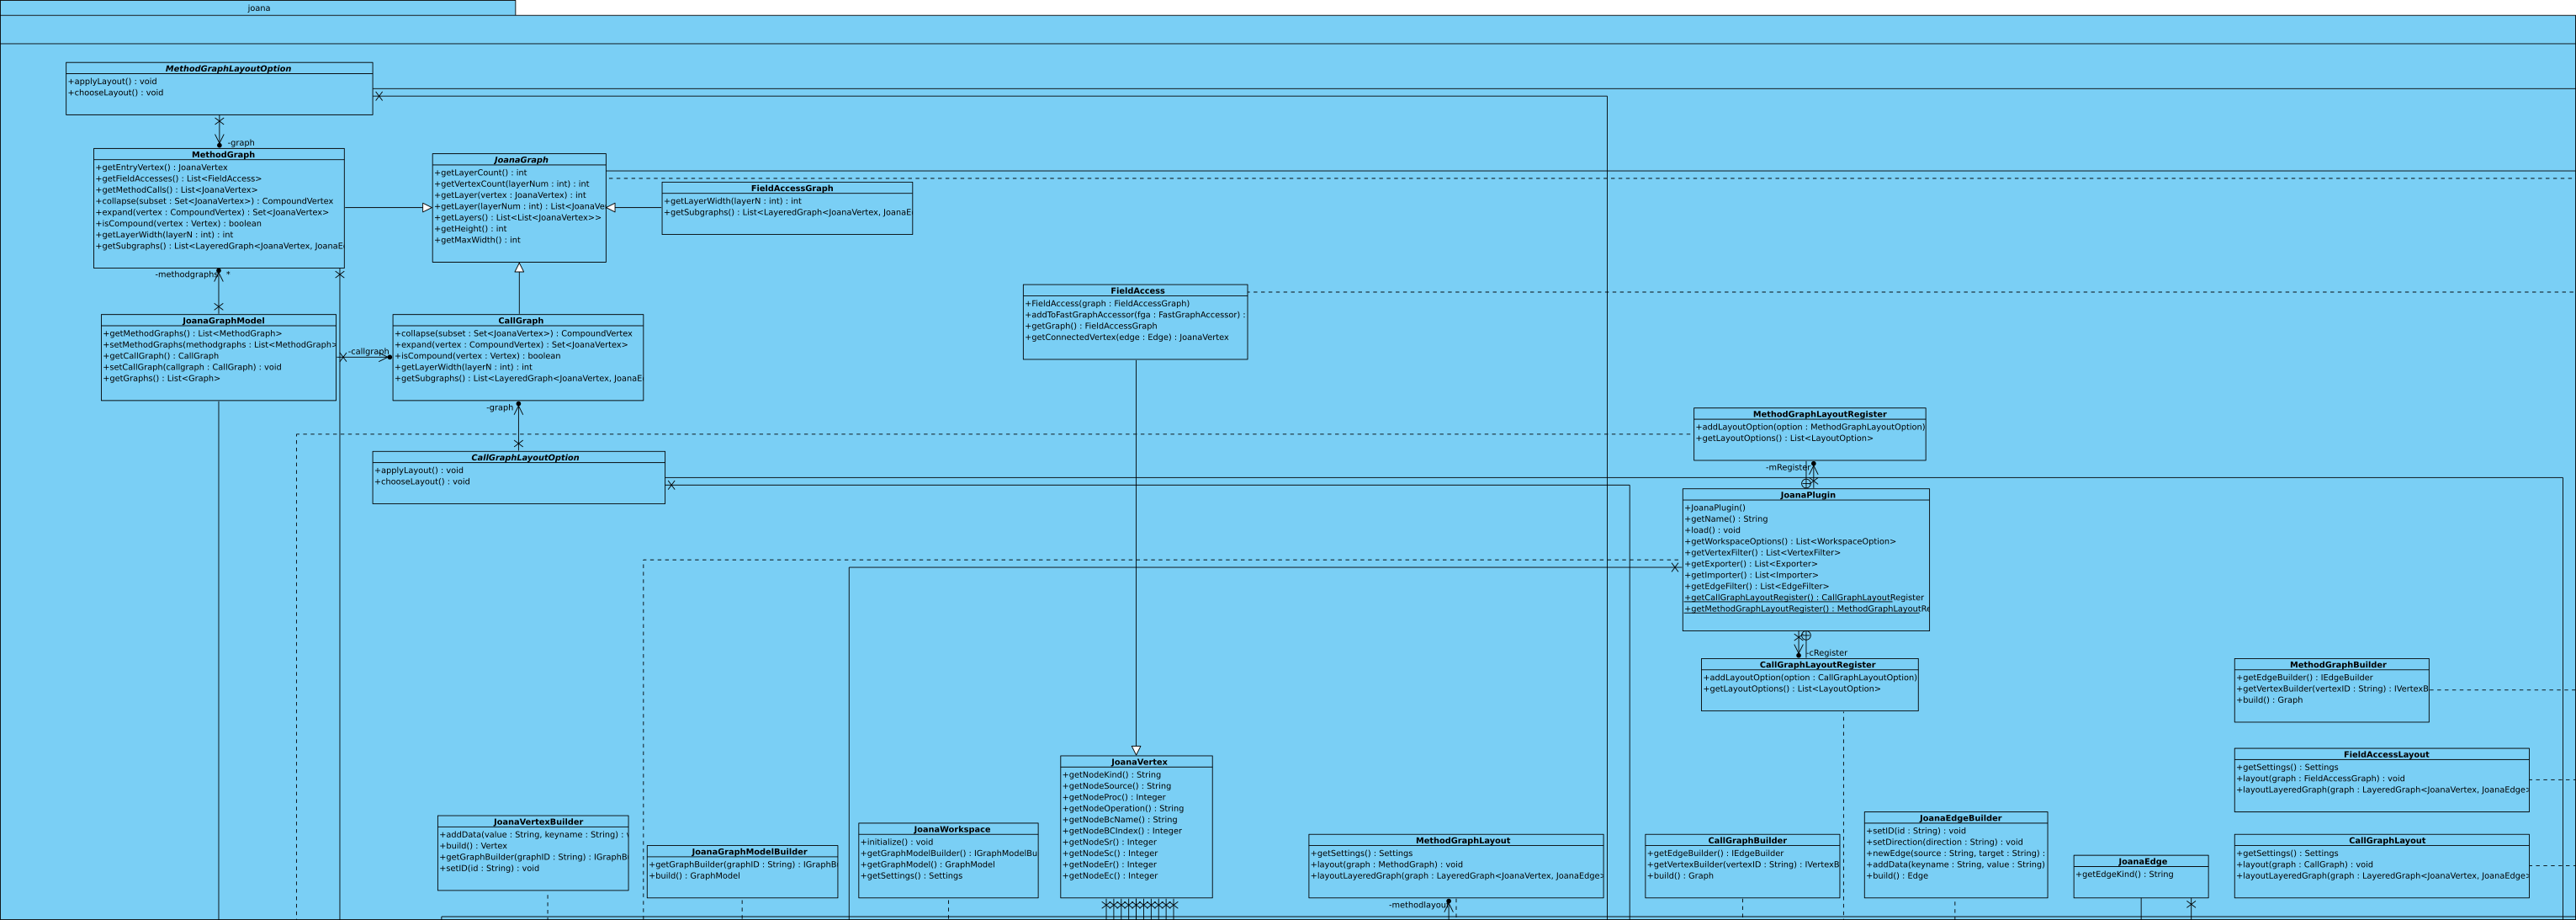
\includegraphics[width=380pt]{resourcen/joana.pdf}
  \caption{Paketübersicht joana}
  \label{fig:packge_joana}
\end{figure}


Das \textbf{joana} Paket bietet Funktionalitäten zum Erstellen von Graphen samt Knoten und Kanten, sowie das Darstellen von \textbf{Methoden}- und \textbf{Callgraphen} in ihren eigenen Layouts.\\
Das \textbf{Workspace} bietet die Möglichkeit zum Einstellen und Speichern von Optionen, speziell für \textbf{JOANA-Graphen}.\\
Zudem ermöglicht das \textbf{joana} Paket die wiedererkennbare Darstellung von Feldzugriffen über das \textbf{FieldAccessLayout}, indem die Zugriffe immer ähnlich dargestellt werden.\\
\textbf{JoanaVertex} und \textbf{JoanaEdge} beinhalten Attribute, welche speziell auf die Eigenschaften abgestimmt sind, welche durch JOANA gesetzt werden.\\
\textbf{Callgraph} und \textbf{Methodengraph}(en) werden in einem speziellen \textbf{JoanaGraphModel} gespeichert.

\chapter{Differenzen zum Pflichtenheft}

\chapter{Klassendiagramme}
\label{ch:klassendiagramme}

Export der JavaDoc aus dem Entwurf. Das Team hat sich auf englische JavaDocs geeinigt, sodass dieses Kapitel in englisch gehalten ist.

\section{Package plugin}{
\label{plugin}\hskip -.05in
\hbox to \hsize{\textit{ Package Contents\hfil Page}}
\vskip .13in
\hbox{{\bf  Interfaces}}
\entityintro{Constraint}{plugin.Constraint}{}
\entityintro{Exporter}{plugin.Exporter}{The exporter interface is used to export a graph from it's internal representation into a specific file.}
\entityintro{FilterSet}{plugin.FilterSet}{A FilterSet is used to collect all available filters for a specific Graph from a workspace.}
\entityintro{Importer}{plugin.Importer}{The importer interface is used to import a graph from a file into the intern representation.}
\entityintro{LayoutAlgorithm}{plugin.LayoutAlgorithm}{An implementations of LayoutAlgorithm takes a graph.}
\entityintro{LayoutRegister}{plugin.LayoutRegister}{Stores a collection of layouts.}
\entityintro{Plugin}{plugin.Plugin}{This is the main entry point for plugins.}
\entityintro{Workspace}{plugin.Workspace}{A workspace contains a set of default actions and options for displaying a specific domain of graphs.}
\vskip .13in
\hbox{{\bf  Classes}}
\entityintro{EdgeFilter}{plugin.EdgeFilter}{This class represents a filter for edges.}
\entityintro{EntryPointOption}{plugin.EntryPointOption}{An entry point option is an abstract superclass for all entry points, where the user can choose one of multiple entry points.}
\entityintro{LayoutOption}{plugin.LayoutOption}{An option for a layout of a specific graph.}
\entityintro{PluginManager}{plugin.PluginManager}{}
\entityintro{VertexFilter}{plugin.VertexFilter}{This Class represents a filter for vertex types.}
\entityintro{WorkspaceOption}{plugin.WorkspaceOption}{This is an option for a}
\vskip .1in
\vskip .1in
\subsection{\label{plugin.Constraint}\index{Constraint@\textit{ Constraint}}Interface Constraint}{
\vskip .1in 
\subsubsection{Declaration}{
\begin{lstlisting}[frame=none]
public interface Constraint
\end{lstlisting}
\subsubsection{Methods}{
\vskip -2em
\begin{itemize}
\item{ 
\index{getName()}
{\bf  getName}\\
\begin{lstlisting}[frame=none]
java.lang.String getName()\end{lstlisting} %end signature
}%end item
\end{itemize}
}
}
\subsection{\label{plugin.Exporter}\index{Exporter@\textit{ Exporter}}Interface Exporter}{
\vskip .1in 
The exporter interface is used to export a graph from it's internal representation into a specific file. For every graph structure given as SerializedGraph/SerializedVertex/SerializedEdge interfaces the implementing class translates it into a FileOutputStream for the given file type, by \texttt{\small getSupportedFileEnding}.\vskip .1in 
\subsubsection{Declaration}{
\begin{lstlisting}[frame=none]
public interface Exporter
\end{lstlisting}
\subsubsection{Methods}{
\vskip -2em
\begin{itemize}
\item{ 
\index{exportGraph(SerializedGraph, FileOutputStream)}
{\bf  exportGraph}\\
\begin{lstlisting}[frame=none]
void exportGraph(graphmodel.SerializedGraph graph,java.io.FileOutputStream filestream)\end{lstlisting} %end signature
\begin{itemize}
\item{
{\bf  Description}

This method writes an \texttt{\small SerializedGraph}{\small 
\refdefined{graphmodel.SerializedGraph}} into an FileOutputStream.
}
\item{
{\bf  Parameters}
  \begin{itemize}
   \item{
\texttt{graph} -- }
   \item{
\texttt{filestream} -- }
  \end{itemize}
}%end item
\end{itemize}
}%end item
\item{ 
\index{getName()}
{\bf  getName}\\
\begin{lstlisting}[frame=none]
java.lang.String getName()\end{lstlisting} %end signature
\begin{itemize}
\item{
{\bf  Description}

Get the name of this importer
}
\item{{\bf  Returns} -- 
 
}%end item
\end{itemize}
}%end item
\item{ 
\index{getSupportedFileEnding()}
{\bf  getSupportedFileEnding}\\
\begin{lstlisting}[frame=none]
java.lang.String getSupportedFileEnding()\end{lstlisting} %end signature
\begin{itemize}
\item{
{\bf  Description}

Get all filetypes which this exporter can parse
}
\item{{\bf  Returns} -- 
 
}%end item
\end{itemize}
}%end item
\end{itemize}
}
}
\subsection{\label{plugin.FilterSet}\index{FilterSet@\textit{ FilterSet}}Interface FilterSet}{
\vskip .1in 
A FilterSet is used to collect all available filters for a specific Graph from a workspace. Just these filters will be displayed to the user for a specific graph\vskip .1in 
\subsubsection{Declaration}{
\begin{lstlisting}[frame=none]
public interface FilterSet
\end{lstlisting}
\subsubsection{Methods}{
\vskip -2em
\begin{itemize}
\item{ 
\index{getEdgeFilter()}
{\bf  getEdgeFilter}\\
\begin{lstlisting}[frame=none]
java.util.List getEdgeFilter()\end{lstlisting} %end signature
\begin{itemize}
\item{
{\bf  Description}

Returns a Set of all available \texttt{\small EdgeFilter}{\small 
\refdefined{plugin.EdgeFilter}}
}
\item{{\bf  Returns} -- 
 
}%end item
\end{itemize}
}%end item
\item{ 
\index{getName()}
{\bf  getName}\\
\begin{lstlisting}[frame=none]
java.lang.String getName()\end{lstlisting} %end signature
\begin{itemize}
\item{
{\bf  Description}

Get the name of this FilterSet
}
\item{{\bf  Returns} -- 
 
}%end item
\end{itemize}
}%end item
\item{ 
\index{getVertexfilter()}
{\bf  getVertexfilter}\\
\begin{lstlisting}[frame=none]
java.util.List getVertexfilter()\end{lstlisting} %end signature
\begin{itemize}
\item{
{\bf  Description}

Returns a Set of all available \texttt{\small VertexFilter}{\small 
\refdefined{plugin.VertexFilter}}.
}
\item{{\bf  Returns} -- 
 
}%end item
\end{itemize}
}%end item
\end{itemize}
}
}
\subsection{\label{plugin.Importer}\index{Importer@\textit{ Importer}}Interface Importer}{
\vskip .1in 
The importer interface is used to import a graph from a file into the intern representation. The main task is to parse a FileInputStream into the Interface of an AbstractGraphModelBuilder. The AbstractGraphModelBuilder will then build the representation.\vskip .1in 
\subsubsection{Declaration}{
\begin{lstlisting}[frame=none]
public interface Importer
\end{lstlisting}
\subsubsection{Methods}{
\vskip -2em
\begin{itemize}
\item{ 
\index{getName()}
{\bf  getName}\\
\begin{lstlisting}[frame=none]
java.lang.String getName()\end{lstlisting} %end signature
\begin{itemize}
\item{
{\bf  Description}

Get the name of this importer
}
\item{{\bf  Returns} -- 
 
}%end item
\end{itemize}
}%end item
\item{ 
\index{getSupportedFileEndings()}
{\bf  getSupportedFileEndings}\\
\begin{lstlisting}[frame=none]
java.util.List getSupportedFileEndings()\end{lstlisting} %end signature
\begin{itemize}
\item{
{\bf  Description}

Get all filetypes which this importer can parse
}
\item{{\bf  Returns} -- 
 
}%end item
\end{itemize}
}%end item
\item{ 
\index{importGraph(IGraphModelBuilder, FileInputStream)}
{\bf  importGraph}\\
\begin{lstlisting}[frame=none]
void importGraph(graphmodel.IGraphModelBuilder builder,java.io.FileInputStream filestream)\end{lstlisting} %end signature
\begin{itemize}
\item{
{\bf  Description}

This method parses an FileInputStream into an AbstractGraphModelBuilder.
}
\item{
{\bf  Parameters}
  \begin{itemize}
   \item{
\texttt{builder} -- }
   \item{
\texttt{filestream} -- }
  \end{itemize}
}%end item
\end{itemize}
}%end item
\end{itemize}
}
}
\subsection{\label{plugin.LayoutAlgorithm}\index{LayoutAlgorithm@\textit{ LayoutAlgorithm}}Interface LayoutAlgorithm}{
\vskip .1in 
An implementations of LayoutAlgorithm takes a graph. It assigns all vertices absolute coordinates and assigns all edges coordinates, they have to pass through. LayoutAlgorithms can be registered with a \texttt{\small LayoutOption}{\small 
\refdefined{plugin.LayoutOption}} at a \texttt{\small LayoutRegister}{\small 
\refdefined{plugin.LayoutRegister}}.\vskip .1in 
\subsubsection{Declaration}{
\begin{lstlisting}[frame=none]
public interface LayoutAlgorithm
\end{lstlisting}
\subsubsection{Methods}{
\vskip -2em
\begin{itemize}
\item{ 
\index{getSettings()}
{\bf  getSettings}\\
\begin{lstlisting}[frame=none]
parameter.Settings getSettings()\end{lstlisting} %end signature
\begin{itemize}
\item{
{\bf  Description}

Get the set of parameters for this instance of the algorithm.
}
\item{{\bf  Returns} -- 
the set of parameters 
}%end item
\end{itemize}
}%end item
\item{ 
\index{layout(G)}
{\bf  layout}\\
\begin{lstlisting}[frame=none]
void layout(graphmodel.Graph graph)\end{lstlisting} %end signature
\begin{itemize}
\item{
{\bf  Description}

Layout the specified Graph.
}
\item{
{\bf  Parameters}
  \begin{itemize}
   \item{
\texttt{graph} -- the graph to layout}
  \end{itemize}
}%end item
\end{itemize}
}%end item
\end{itemize}
}
}
\subsection{\label{plugin.LayoutRegister}\index{LayoutRegister@\textit{ LayoutRegister}}Interface LayoutRegister}{
\vskip .1in 
Stores a collection of layouts. This\vskip .1in 
\subsubsection{Declaration}{
\begin{lstlisting}[frame=none]
public interface LayoutRegister
\end{lstlisting}
\subsubsection{Methods}{
\vskip -2em
\begin{itemize}
\item{ 
\index{addLayoutOption(E)}
{\bf  addLayoutOption}\\
\begin{lstlisting}[frame=none]
void addLayoutOption(LayoutOption option)\end{lstlisting} %end signature
}%end item
\item{ 
\index{getLayoutOptions()}
{\bf  getLayoutOptions}\\
\begin{lstlisting}[frame=none]
java.util.List getLayoutOptions()\end{lstlisting} %end signature
}%end item
\end{itemize}
}
}
\subsection{\label{plugin.Plugin}\index{Plugin@\textit{ Plugin}}Interface Plugin}{
\vskip .1in 
This is the main entry point for plugins. Plugins have to register their content extensions via this interface. The plugin manager will load classes implementing this interface with a service loader, when they are correctly described in the plugins META-INF.\vskip .1in 
\subsubsection{Declaration}{
\begin{lstlisting}[frame=none]
public interface Plugin
\end{lstlisting}
\subsubsection{Methods}{
\vskip -2em
\begin{itemize}
\item{ 
\index{getEdgeFilter()}
{\bf  getEdgeFilter}\\
\begin{lstlisting}[frame=none]
java.util.List getEdgeFilter()\end{lstlisting} %end signature
\begin{itemize}
\item{
{\bf  Description}

Returns all by the plugin provided \texttt{\small EdgeFilter}{\small 
\refdefined{plugin.EdgeFilter}}. If none are provided returns \texttt{\small null} or an empty list.
}
\item{{\bf  Returns} -- 
the list of provided edge filter 
}%end item
\end{itemize}
}%end item
\item{ 
\index{getName()}
{\bf  getName}\\
\begin{lstlisting}[frame=none]
java.lang.String getName()\end{lstlisting} %end signature
\begin{itemize}
\item{
{\bf  Description}

Returns the name of the plugin. Uniqueness can't be assumed.
}
\item{{\bf  Returns} -- 
the name of the plugin 
}%end item
\end{itemize}
}%end item
\item{ 
\index{getVertexFilter()}
{\bf  getVertexFilter}\\
\begin{lstlisting}[frame=none]
java.util.List getVertexFilter()\end{lstlisting} %end signature
\begin{itemize}
\item{
{\bf  Description}

Returns all by the plugin provided \texttt{\small VertexFilter}{\small 
\refdefined{plugin.VertexFilter}}. If none are provided returns \texttt{\small null} or an empty list.
}
\item{{\bf  Returns} -- 
the list of provided vertex filter 
}%end item
\end{itemize}
}%end item
\item{ 
\index{getWorkspaceOptions()}
{\bf  getWorkspaceOptions}\\
\begin{lstlisting}[frame=none]
java.util.List getWorkspaceOptions()\end{lstlisting} %end signature
\begin{itemize}
\item{
{\bf  Description}

Returns all provided by the plugin \texttt{\small WorkspaceOption}{\small 
\refdefined{plugin.WorkspaceOption}}. If none are provided returns \texttt{\small null} or an empty list.
}
\item{{\bf  Returns} -- 
The list of provided workspace options 
}%end item
\end{itemize}
}%end item
\item{ 
\index{load()}
{\bf  load}\\
\begin{lstlisting}[frame=none]
void load()\end{lstlisting} %end signature
\begin{itemize}
\item{
{\bf  Description}

Called after all plugins have been constructed. "Inter-Plugin" communication, like registering of layouts for graphs in other plugins should be executed in here.
}
\end{itemize}
}%end item
\end{itemize}
}
}
\subsection{\label{plugin.Workspace}\index{Workspace@\textit{ Workspace}}Interface Workspace}{
\vskip .1in 
A workspace contains a set of default actions and options for displaying a specific domain of graphs. The workspace manages the graphs instantiation through providing an \texttt{\small IGraphModelBuilder}{\small 
\refdefined{graphmodel.IGraphModelBuilder}}. He also provides a list of layout options for graphs in his model.\vskip .1in 
\subsubsection{Declaration}{
\begin{lstlisting}[frame=none]
public interface Workspace
\end{lstlisting}
\subsubsection{Methods}{
\vskip -2em
\begin{itemize}
\item{ 
\index{getGraphModel()}
{\bf  getGraphModel}\\
\begin{lstlisting}[frame=none]
graphmodel.GraphModel getGraphModel()\end{lstlisting} %end signature
\begin{itemize}
\item{
{\bf  Description}

Returns the \texttt{\small GraphModel}{\small 
\refdefined{graphmodel.GraphModel}} stored in the workspace.
}
\item{{\bf  Returns} -- 
the graph model 
}%end item
\end{itemize}
}%end item
\item{ 
\index{getGraphModelBuilder()}
{\bf  getGraphModelBuilder}\\
\begin{lstlisting}[frame=none]
graphmodel.IGraphModelBuilder getGraphModelBuilder()\end{lstlisting} %end signature
\begin{itemize}
\item{
{\bf  Description}

Returns a builder to build a graph model in this workspace.
}
\item{{\bf  Returns} -- 
the builder 
}%end item
\end{itemize}
}%end item
\item{ 
\index{getSettings()}
{\bf  getSettings}\\
\begin{lstlisting}[frame=none]
parameter.Settings getSettings()\end{lstlisting} %end signature
\begin{itemize}
\item{
{\bf  Description}

Returns a set of parameters to initialize this workspace. When the settings have been adjusted, the client has to call \texttt{\small initialize()}. To initialize the workspace with the settings.
}
\item{{\bf  Returns} -- 
the settings 
}%end item
\end{itemize}
}%end item
\item{ 
\index{initialize()}
{\bf  initialize}\\
\begin{lstlisting}[frame=none]
void initialize()\end{lstlisting} %end signature
\begin{itemize}
\item{
{\bf  Description}

Initializes this workspace with the settings if they have not been adjusted. If the settings have not been adjusted, default values will be used.
}
\end{itemize}
}%end item
\end{itemize}
}
}
\subsection{\label{plugin.EdgeFilter}\index{EdgeFilter}Class EdgeFilter}{
\vskip .1in 
This class represents a filter for edges. To check if an edge passes through this filter, the client can specify it in \texttt{\small matches(Edge edge)}.\vskip .1in 
\subsubsection{Declaration}{
\begin{lstlisting}[frame=none]
public abstract class EdgeFilter
 extends java.lang.Object\end{lstlisting}
\subsubsection{Constructors}{
\vskip -2em
\begin{itemize}
\item{ 
\index{EdgeFilter()}
{\bf  EdgeFilter}\\
\begin{lstlisting}[frame=none]
public EdgeFilter()\end{lstlisting} %end signature
}%end item
\end{itemize}
}
\subsubsection{Methods}{
\vskip -2em
\begin{itemize}
\item{ 
\index{getName()}
{\bf  getName}\\
\begin{lstlisting}[frame=none]
public java.lang.String getName()\end{lstlisting} %end signature
\begin{itemize}
\item{
{\bf  Description}

Returns the name of the filter.
}
\item{{\bf  Returns} -- 
the name of the filter 
}%end item
\end{itemize}
}%end item
\item{ 
\index{matches(Edge)}
{\bf  matches}\\
\begin{lstlisting}[frame=none]
public abstract boolean matches(graphmodel.Edge toMatch)\end{lstlisting} %end signature
\begin{itemize}
\item{
{\bf  Description}

This method checks if an edge matches this Filter. It will compare specified parameters of the edge with the defined parameters of this filter.
}
\item{
{\bf  Parameters}
  \begin{itemize}
   \item{
\texttt{toMatch} -- the edge which should be checked}
  \end{itemize}
}%end item
\item{{\bf  Returns} -- 
true if the edge matches this Filter, otherwise false 
}%end item
\end{itemize}
}%end item
\item{ 
\index{setName(String)}
{\bf  setName}\\
\begin{lstlisting}[frame=none]
public void setName(java.lang.String name)\end{lstlisting} %end signature
\begin{itemize}
\item{
{\bf  Description}

Sets the name of the filter.
}
\item{
{\bf  Parameters}
  \begin{itemize}
   \item{
\texttt{name} -- the name of the filter}
  \end{itemize}
}%end item
\end{itemize}
}%end item
\end{itemize}
}
}
\subsection{\label{plugin.EntryPointOption}\index{EntryPointOption}Class EntryPointOption}{
\vskip .1in 
An entry point option is an abstract superclass for all entry points, where the user can choose one of multiple entry points. Entry point options should allow a categorical overview for the entry point, to enable the client to differentiate the option from other options. Additionally a method for should be provided which can be executed when the client wants to select an option.\vskip .1in 
\subsubsection{Declaration}{
\begin{lstlisting}[frame=none]
public abstract class EntryPointOption
 extends java.lang.Object\end{lstlisting}
\subsubsection{All known subclasses}{WorkspaceOption\small{\refdefined{plugin.WorkspaceOption}}, LayoutOption\small{\refdefined{plugin.LayoutOption}}}
\subsubsection{Constructors}{
\vskip -2em
\begin{itemize}
\item{ 
\index{EntryPointOption()}
{\bf  EntryPointOption}\\
\begin{lstlisting}[frame=none]
public EntryPointOption()\end{lstlisting} %end signature
}%end item
\end{itemize}
}
\subsubsection{Methods}{
\vskip -2em
\begin{itemize}
\item{ 
\index{getID()}
{\bf  getID}\\
\begin{lstlisting}[frame=none]
public java.lang.String getID()\end{lstlisting} %end signature
\begin{itemize}
\item{
{\bf  Description}

The id of an entry point should be an acronym of it's name.
}
\item{{\bf  Returns} -- 
the id 
}%end item
\end{itemize}
}%end item
\item{ 
\index{getName()}
{\bf  getName}\\
\begin{lstlisting}[frame=none]
public java.lang.String getName()\end{lstlisting} %end signature
\begin{itemize}
\item{
{\bf  Description}

Returns the name of the entry point option. This name can be displayed when displaying multiple options
}
\item{{\bf  Returns} -- 
the name of the entry point 
}%end item
\end{itemize}
}%end item
\item{ 
\index{setID(String)}
{\bf  setID}\\
\begin{lstlisting}[frame=none]
protected void setID(java.lang.String id)\end{lstlisting} %end signature
\begin{itemize}
\item{
{\bf  Description}

Sets the id of the entry point. The id should be an acronym of the name.
}
\item{
{\bf  Parameters}
  \begin{itemize}
   \item{
\texttt{id} -- the id of the entry point.}
  \end{itemize}
}%end item
\end{itemize}
}%end item
\item{ 
\index{setName(String)}
{\bf  setName}\\
\begin{lstlisting}[frame=none]
protected void setName(java.lang.String name)\end{lstlisting} %end signature
\begin{itemize}
\item{
{\bf  Description}

Sets the name of the entry point
}
\item{
{\bf  Parameters}
  \begin{itemize}
   \item{
\texttt{name} -- the name of the entry point}
  \end{itemize}
}%end item
\end{itemize}
}%end item
\end{itemize}
}
}
\subsection{\label{plugin.LayoutOption}\index{LayoutOption}Class LayoutOption}{
\vskip .1in 
An option for a layout of a specific graph. Workspaces can return these for a specific graph. The client can then decide between one ore more LayoutOptions When selected the layout will be applied to the graph.\vskip .1in 
\subsubsection{Declaration}{
\begin{lstlisting}[frame=none]
public abstract class LayoutOption
 extends plugin.EntryPointOption implements java.lang.Cloneable\end{lstlisting}
\subsubsection{Constructors}{
\vskip -2em
\begin{itemize}
\item{ 
\index{LayoutOption()}
{\bf  LayoutOption}\\
\begin{lstlisting}[frame=none]
public LayoutOption()\end{lstlisting} %end signature
}%end item
\end{itemize}
}
\subsubsection{Methods}{
\vskip -2em
\begin{itemize}
\item{ 
\index{applyLayout()}
{\bf  applyLayout}\\
\begin{lstlisting}[frame=none]
public abstract void applyLayout()\end{lstlisting} %end signature
\begin{itemize}
\item{
{\bf  Description}

This should execute the layout on the graph, which should be specified on construction, or in beforehand. The settings, which are accessible over \texttt{\small getSettings()} will be used to instantiate the LayoutAlgorithm.
}
\end{itemize}
}%end item
\item{ 
\index{chooseLayout()}
{\bf  chooseLayout}\\
\begin{lstlisting}[frame=none]
public abstract void chooseLayout()\end{lstlisting} %end signature
\begin{itemize}
\item{
{\bf  Description}

Called when this layout option is chosen. This allows the layout option to prepare the actual LayoutAlgorithm.
}
\end{itemize}
}%end item
\item{ 
\index{getSettings()}
{\bf  getSettings}\\
\begin{lstlisting}[frame=none]
public abstract parameter.Settings getSettings()\end{lstlisting} %end signature
\begin{itemize}
\item{
{\bf  Description}

Get the set of parameters for an algorithm of this option. \texttt{\small choose()} has to be called up front.
}
\item{{\bf  Returns} -- 
the set of parameters 
}%end item
\end{itemize}
}%end item
\end{itemize}
}
}
\subsection{\label{plugin.PluginManager}\index{PluginManager}Class PluginManager}{
\vskip .1in 
\subsubsection{Declaration}{
\begin{lstlisting}[frame=none]
public class PluginManager
 extends java.lang.Object\end{lstlisting}
\subsubsection{Methods}{
\vskip -2em
\begin{itemize}
\item{ 
\index{addExporter(Exporter)}
{\bf  addExporter}\\
\begin{lstlisting}[frame=none]
public void addExporter(Exporter exporter)\end{lstlisting} %end signature
}%end item
\item{ 
\index{addImporter(Importer)}
{\bf  addImporter}\\
\begin{lstlisting}[frame=none]
public void addImporter(Importer importer)\end{lstlisting} %end signature
}%end item
\item{ 
\index{getEdgeFilter()}
{\bf  getEdgeFilter}\\
\begin{lstlisting}[frame=none]
public java.util.List getEdgeFilter()\end{lstlisting} %end signature
\begin{itemize}
\item{
{\bf  Description}

Returns a list of all edge filter provided by plugins.
}
\item{{\bf  Returns} -- 
a list of all edge filter 
}%end item
\end{itemize}
}%end item
\item{ 
\index{getExporters()}
{\bf  getExporters}\\
\begin{lstlisting}[frame=none]
public java.util.List getExporters()\end{lstlisting} %end signature
}%end item
\item{ 
\index{getImporters()}
{\bf  getImporters}\\
\begin{lstlisting}[frame=none]
public java.util.List getImporters()\end{lstlisting} %end signature
}%end item
\item{ 
\index{getPluginManager()}
{\bf  getPluginManager}\\
\begin{lstlisting}[frame=none]
public static PluginManager getPluginManager()\end{lstlisting} %end signature
\begin{itemize}
\item{
{\bf  Description}

Returns the singleton instance of the plugin manager.
}
\item{{\bf  Returns} -- 
the plugin manager 
}%end item
\end{itemize}
}%end item
\item{ 
\index{getPlugins()}
{\bf  getPlugins}\\
\begin{lstlisting}[frame=none]
public java.util.List getPlugins()\end{lstlisting} %end signature
\begin{itemize}
\item{
{\bf  Description}

Returns a list of all plugins loaded by the ServiceLoader.
}
\item{{\bf  Returns} -- 
all loaded plugins 
}%end item
\end{itemize}
}%end item
\item{ 
\index{getVertexFilter()}
{\bf  getVertexFilter}\\
\begin{lstlisting}[frame=none]
public java.util.List getVertexFilter()\end{lstlisting} %end signature
\begin{itemize}
\item{
{\bf  Description}

Returns all vertex filter provided by plugins.
}
\item{{\bf  Returns} -- 
a list of all vertex filter 
}%end item
\end{itemize}
}%end item
\item{ 
\index{getWorkspaceOptions()}
{\bf  getWorkspaceOptions}\\
\begin{lstlisting}[frame=none]
public java.util.List getWorkspaceOptions()\end{lstlisting} %end signature
\begin{itemize}
\item{
{\bf  Description}

Returns all \texttt{\small WorkspaceOption}{\small 
\refdefined{plugin.WorkspaceOption}}s provided by plugins.
}
\item{{\bf  Returns} -- 
a list of all workspace options 
}%end item
\end{itemize}
}%end item
\end{itemize}
}
}
\subsection{\label{plugin.VertexFilter}\index{VertexFilter}Class VertexFilter}{
\vskip .1in 
This Class represents a filter for vertex types. The type of the vertex can be specified through different parameters.\vskip .1in 
\subsubsection{Declaration}{
\begin{lstlisting}[frame=none]
public class VertexFilter
 extends java.lang.Object\end{lstlisting}
\subsubsection{Constructors}{
\vskip -2em
\begin{itemize}
\item{ 
\index{VertexFilter()}
{\bf  VertexFilter}\\
\begin{lstlisting}[frame=none]
public VertexFilter()\end{lstlisting} %end signature
}%end item
\end{itemize}
}
\subsubsection{Methods}{
\vskip -2em
\begin{itemize}
\item{ 
\index{getName()}
{\bf  getName}\\
\begin{lstlisting}[frame=none]
public java.lang.String getName()\end{lstlisting} %end signature
\begin{itemize}
\item{
{\bf  Description}

Getter of name
}
\end{itemize}
}%end item
\item{ 
\index{matches(Vertex)}
{\bf  matches}\\
\begin{lstlisting}[frame=none]
public boolean matches(graphmodel.Vertex toMatch)\end{lstlisting} %end signature
\begin{itemize}
\item{
{\bf  Description}

This method checks if an vertex matches this Filter. It will compare specified parameters of the vertex with the defined parameters of this filter.
}
\item{
{\bf  Parameters}
  \begin{itemize}
   \item{
\texttt{toMatch} -- the vertex which should be checked}
  \end{itemize}
}%end item
\item{{\bf  Returns} -- 
true if the edge matches this Filter, otherwise false 
}%end item
\end{itemize}
}%end item
\item{ 
\index{setName(String)}
{\bf  setName}\\
\begin{lstlisting}[frame=none]
public void setName(java.lang.String name)\end{lstlisting} %end signature
\begin{itemize}
\item{
{\bf  Description}

Setter of name
}
\end{itemize}
}%end item
\end{itemize}
}
}
\subsection{\label{plugin.WorkspaceOption}\index{WorkspaceOption}Class WorkspaceOption}{
\vskip .1in 
This is an option for a\vskip .1in 
\subsubsection{Declaration}{
\begin{lstlisting}[frame=none]
public abstract class WorkspaceOption
 extends plugin.EntryPointOption\end{lstlisting}
\subsubsection{Constructors}{
\vskip -2em
\begin{itemize}
\item{ 
\index{WorkspaceOption()}
{\bf  WorkspaceOption}\\
\begin{lstlisting}[frame=none]
public WorkspaceOption()\end{lstlisting} %end signature
}%end item
\end{itemize}
}
\subsubsection{Methods}{
\vskip -2em
\begin{itemize}
\item{ 
\index{getInstance()}
{\bf  getInstance}\\
\begin{lstlisting}[frame=none]
public abstract Workspace getInstance()\end{lstlisting} %end signature
\begin{itemize}
\item{
{\bf  Description}

Creates an instance of the workspace with the earlier adjusted Settings
}
\item{{\bf  Returns} -- 
a workspace 
}%end item
\end{itemize}
}%end item
\item{ 
\index{getSettings()}
{\bf  getSettings}\\
\begin{lstlisting}[frame=none]
public abstract parameter.Settings getSettings()\end{lstlisting} %end signature
\begin{itemize}
\item{
{\bf  Description}

Returns a set of parameters to initialize a workspace for this. When the settings have been adjusted, the client has to call \texttt{\small getInstance()}, to get an instance of the workspace with the settings.
}
\item{{\bf  Returns} -- 
the settings 
}%end item
\end{itemize}
}%end item
\end{itemize}
}
}
}
\printindex


%\section*{Class Hierarchy}{
\thispagestyle{empty}
\markboth{Class Hierarchy}{Class Hierarchy}
\addcontentsline{toc}{section}{Class Hierarchy}
\subsection*{Classes}
{\raggedright
\hspace{0.0cm} $\bullet$ java.lang.Object {\tiny \refdefined{java.lang.Object}} \\
\hspace{1.0cm} $\bullet$ gui.GraphViewEventHandler {\tiny \refdefined{gui.GraphViewEventHandler}} \\
\hspace{1.0cm} $\bullet$ javafx.application.Application {\tiny \refdefined{javafx.application.Application}} \\
\hspace{2.0cm} $\bullet$ gui.GAnsApplication {\tiny \refdefined{gui.GAnsApplication}} \\
\hspace{1.0cm} $\bullet$ javafx.scene.Node {\tiny \refdefined{javafx.scene.Node}} \\
\hspace{2.0cm} $\bullet$ javafx.scene.Parent {\tiny \refdefined{javafx.scene.Parent}} \\
\hspace{3.0cm} $\bullet$ javafx.scene.layout.Region {\tiny \refdefined{javafx.scene.layout.Region}} \\
\hspace{4.0cm} $\bullet$ javafx.scene.control.Control {\tiny \refdefined{javafx.scene.control.Control}} \\
\hspace{5.0cm} $\bullet$ javafx.scene.control.TableView {\tiny \refdefined{javafx.scene.control.TableView}} \\
\hspace{6.0cm} $\bullet$ gui.InformationView {\tiny \refdefined{gui.InformationView}} \\
\hspace{5.0cm} $\bullet$ javafx.scene.control.TreeView {\tiny \refdefined{javafx.scene.control.TreeView}} \\
\hspace{6.0cm} $\bullet$ gui.StructureView {\tiny \refdefined{gui.StructureView}} \\
\hspace{4.0cm} $\bullet$ javafx.scene.layout.Pane {\tiny \refdefined{javafx.scene.layout.Pane}} \\
\hspace{5.0cm} $\bullet$ gui.GraphView {\tiny \refdefined{gui.GraphView}} \\
\hspace{5.0cm} $\bullet$ javafx.scene.layout.StackPane {\tiny \refdefined{javafx.scene.layout.StackPane}} \\
\hspace{6.0cm} $\bullet$ gui.VertexShape {\tiny \refdefined{gui.VertexShape}} \\
}
}
\section{Package gui}{
\label{gui}\hskip -.05in
\hbox to \hsize{\textit{ Package Contents\hfil Page}}
\vskip .13in
\hbox{{\bf  Classes}}
\entityintro{GAnsApplication}{gui.GAnsApplication}{Main application of GAns.}
\entityintro{GraphView}{gui.GraphView}{A view used for showing and creating a graph in GAns.}
\entityintro{GraphViewEventHandler}{gui.GraphViewEventHandler}{GraphViewEventHandler provides listeners for making the \texttt{\small GraphView}{\small 
\refdefined{gui.GraphView}} draggable and zoomable.}
\entityintro{InformationView}{gui.InformationView}{The InformationView shows a given set of properties from the selected vertices in the \texttt{\small GraphView}{\small 
\refdefined{gui.GraphView}}.}
\entityintro{StructureView}{gui.StructureView}{The StructureView regulates the access and representation of the elements in the StructreView of GAns.}
\entityintro{VertexShape}{gui.VertexShape}{A graphical representation of a node with a text inside of it.}
\vskip .1in
\vskip .1in
\subsection{\label{gui.GAnsApplication}\index{GAnsApplication}Class GAnsApplication}{
\vskip .1in 
Main application of GAns.\vskip .1in 
\subsubsection{Declaration}{
\begin{lstlisting}[frame=none]
public class GAnsApplication
 extends javafx.application.Application\end{lstlisting}
\subsubsection{Constructor summary}{
\begin{verse}
{\bf GAnsApplication()} \\
\end{verse}
}
\subsubsection{Method summary}{
\begin{verse}
{\bf main(String\lbrack \rbrack )} Main method.\\
{\bf start(Stage)} \\
\end{verse}
}
\subsubsection{Constructors}{
\vskip -2em
\begin{itemize}
\item{ 
\index{GAnsApplication()}
{\bf  GAnsApplication}\\
\begin{lstlisting}[frame=none]
public GAnsApplication()\end{lstlisting} %end signature
}%end item
\end{itemize}
}
\subsubsection{Methods}{
\vskip -2em
\begin{itemize}
\item{ 
\index{main(String\lbrack \rbrack )}
{\bf  main}\\
\begin{lstlisting}[frame=none]
public static void main(java.lang.String[] args)\end{lstlisting} %end signature
\begin{itemize}
\item{
{\bf  Description}

Main method.
}
\item{
{\bf  Parameters}
  \begin{itemize}
   \item{
\texttt{args} -- Arguments.}
  \end{itemize}
}%end item
\end{itemize}
}%end item
\item{ 
\index{start(Stage)}
{\bf  start}\\
\begin{lstlisting}[frame=none]
public abstract void start(javafx.stage.Stage arg0) throws java.lang.Exception\end{lstlisting} %end signature
}%end item
\end{itemize}
}
\subsubsection{Members inherited from class Application }{
\texttt{javafx.application.Application} {\small 
\refdefined{javafx.application.Application}}
{\small 

\vskip -2em
\begin{itemize}
\item{\vskip -1.5ex 
\texttt{public final HostServices {\bf  getHostServices}()
}%end signature
}%end item
\item{\vskip -1.5ex 
\texttt{public final Application.Parameters {\bf  getParameters}()
}%end signature
}%end item
\item{\vskip -1.5ex 
\texttt{public static String {\bf  getUserAgentStylesheet}()
}%end signature
}%end item
\item{\vskip -1.5ex 
\texttt{public void {\bf  init}() throws java.lang.Exception
}%end signature
}%end item
\item{\vskip -1.5ex 
\texttt{public static void {\bf  launch}(\texttt{java.lang.Class} {\bf  arg0},
\texttt{java.lang.String\lbrack \rbrack } {\bf  arg1})
}%end signature
}%end item
\item{\vskip -1.5ex 
\texttt{public static void {\bf  launch}(\texttt{java.lang.String\lbrack \rbrack } {\bf  arg0})
}%end signature
}%end item
\item{\vskip -1.5ex 
\texttt{public final void {\bf  notifyPreloader}(\texttt{Preloader.PreloaderNotification} {\bf  arg0})
}%end signature
}%end item
\item{\vskip -1.5ex 
\texttt{public static void {\bf  setUserAgentStylesheet}(\texttt{java.lang.String} {\bf  arg0})
}%end signature
}%end item
\item{\vskip -1.5ex 
\texttt{public abstract void {\bf  start}(\texttt{javafx.stage.Stage} {\bf  arg0}) throws java.lang.Exception
}%end signature
}%end item
\item{\vskip -1.5ex 
\texttt{public void {\bf  stop}() throws java.lang.Exception
}%end signature
}%end item
\item{\vskip -1.5ex 
\texttt{public static final {\bf  STYLESHEET\_CASPIAN}}%end signature
}%end item
\item{\vskip -1.5ex 
\texttt{public static final {\bf  STYLESHEET\_MODENA}}%end signature
}%end item
\end{itemize}
}
}
\subsection{\label{gui.GraphView}\index{GraphView}Class GraphView}{
\vskip .1in 
A view used for showing and creating a graph in GAns. It supports zooming and other general navigation features.\vskip .1in 
\subsubsection{Declaration}{
\begin{lstlisting}[frame=none]
public class GraphView
 extends javafx.scene.layout.Pane\end{lstlisting}
\subsubsection{Constructor summary}{
\begin{verse}
{\bf GraphView()} Constructor.\\
\end{verse}
}
\subsubsection{Method summary}{
\begin{verse}
{\bf addGrid()} Adds a grid to the GraphView, on which the dragging can be mapped.\\
{\bf addVertex(double, double, String)} Adds a single vertex in the GraphView.\\
{\bf getScale()} Returns the scale on which the GraphView currently is.\\
{\bf setGraph()} Sets a graph.\\
{\bf setPivot(double, double)} Sets the pivot so the scrolling follows the mouse position on the GraphView.\\
{\bf setScale(double)} Sets the scale of the GraphView.\\
\end{verse}
}
\subsubsection{Constructors}{
\vskip -2em
\begin{itemize}
\item{ 
\index{GraphView()}
{\bf  GraphView}\\
\begin{lstlisting}[frame=none]
public GraphView()\end{lstlisting} %end signature
\begin{itemize}
\item{
{\bf  Description}

Constructor.
}
\end{itemize}
}%end item
\end{itemize}
}
\subsubsection{Methods}{
\vskip -2em
\begin{itemize}
\item{ 
\index{addGrid()}
{\bf  addGrid}\\
\begin{lstlisting}[frame=none]
public void addGrid()\end{lstlisting} %end signature
\begin{itemize}
\item{
{\bf  Description}

Adds a grid to the GraphView, on which the dragging can be mapped.
}
\end{itemize}
}%end item
\item{ 
\index{addVertex(double, double, String)}
{\bf  addVertex}\\
\begin{lstlisting}[frame=none]
public void addVertex(double x,double y,java.lang.String text)\end{lstlisting} %end signature
\begin{itemize}
\item{
{\bf  Description}

Adds a single vertex in the GraphView.
}
\item{
{\bf  Parameters}
  \begin{itemize}
   \item{
\texttt{x} -- The x position in the view.}
   \item{
\texttt{y} -- The y position in the view.}
   \item{
\texttt{Text} -- The text of the vertex.}
  \end{itemize}
}%end item
\end{itemize}
}%end item
\item{ 
\index{getScale()}
{\bf  getScale}\\
\begin{lstlisting}[frame=none]
public double getScale()\end{lstlisting} %end signature
\begin{itemize}
\item{
{\bf  Description}

Returns the scale on which the GraphView currently is.
}
\item{{\bf  Returns} -- 
The scale of the GraphView. 
}%end item
\end{itemize}
}%end item
\item{ 
\index{setGraph()}
{\bf  setGraph}\\
\begin{lstlisting}[frame=none]
public void setGraph()\end{lstlisting} %end signature
\begin{itemize}
\item{
{\bf  Description}

Sets a graph. Every element in the graph will be generated and then shown.
}
\item{
{\bf  Parameters}
  \begin{itemize}
   \item{
\texttt{graph} -- The graph to be visualized in the view.}
  \end{itemize}
}%end item
\end{itemize}
}%end item
\item{ 
\index{setPivot(double, double)}
{\bf  setPivot}\\
\begin{lstlisting}[frame=none]
public void setPivot(double x,double y)\end{lstlisting} %end signature
\begin{itemize}
\item{
{\bf  Description}

Sets the pivot so the scrolling follows the mouse position on the GraphView.
}
\item{
{\bf  Parameters}
  \begin{itemize}
   \item{
\texttt{x} -- }
   \item{
\texttt{y} -- }
  \end{itemize}
}%end item
\end{itemize}
}%end item
\item{ 
\index{setScale(double)}
{\bf  setScale}\\
\begin{lstlisting}[frame=none]
public void setScale(double scale)\end{lstlisting} %end signature
\begin{itemize}
\item{
{\bf  Description}

Sets the scale of the GraphView.
}
\item{
{\bf  Parameters}
  \begin{itemize}
   \item{
\texttt{scale} -- The scale of the GraphView.}
  \end{itemize}
}%end item
\end{itemize}
}%end item
\end{itemize}
}
\subsubsection{Members inherited from class Pane }{
\texttt{javafx.scene.layout.Pane} {\small 
\refdefined{javafx.scene.layout.Pane}}
{\small 

\vskip -2em
\begin{itemize}
\item{\vskip -1.5ex 
\texttt{public ObservableList {\bf  getChildren}()
}%end signature
}%end item
\end{itemize}
}
\subsubsection{Members inherited from class Region }{
\texttt{javafx.scene.layout.Region} {\small 
\refdefined{javafx.scene.layout.Region}}
{\small 

\vskip -2em
\begin{itemize}
\item{\vskip -1.5ex 
\texttt{public final ObjectProperty {\bf  backgroundProperty}()
}%end signature
}%end item
\item{\vskip -1.5ex 
\texttt{public final ObjectProperty {\bf  borderProperty}()
}%end signature
}%end item
\item{\vskip -1.5ex 
\texttt{public final BooleanProperty {\bf  cacheShapeProperty}()
}%end signature
}%end item
\item{\vskip -1.5ex 
\texttt{public final BooleanProperty {\bf  centerShapeProperty}()
}%end signature
}%end item
\item{\vskip -1.5ex 
\texttt{protected double {\bf  computeMaxHeight}(\texttt{double} {\bf  arg0})
}%end signature
}%end item
\item{\vskip -1.5ex 
\texttt{protected double {\bf  computeMaxWidth}(\texttt{double} {\bf  arg0})
}%end signature
}%end item
\item{\vskip -1.5ex 
\texttt{protected double {\bf  computeMinHeight}(\texttt{double} {\bf  arg0})
}%end signature
}%end item
\item{\vskip -1.5ex 
\texttt{protected double {\bf  computeMinWidth}(\texttt{double} {\bf  arg0})
}%end signature
}%end item
\item{\vskip -1.5ex 
\texttt{protected double {\bf  computePrefHeight}(\texttt{double} {\bf  arg0})
}%end signature
}%end item
\item{\vskip -1.5ex 
\texttt{protected double {\bf  computePrefWidth}(\texttt{double} {\bf  arg0})
}%end signature
}%end item
\item{\vskip -1.5ex 
\texttt{public final Background {\bf  getBackground}()
}%end signature
}%end item
\item{\vskip -1.5ex 
\texttt{public final Border {\bf  getBorder}()
}%end signature
}%end item
\item{\vskip -1.5ex 
\texttt{public static List {\bf  getClassCssMetaData}()
}%end signature
}%end item
\item{\vskip -1.5ex 
\texttt{public List {\bf  getCssMetaData}()
}%end signature
}%end item
\item{\vskip -1.5ex 
\texttt{public final double {\bf  getHeight}()
}%end signature
}%end item
\item{\vskip -1.5ex 
\texttt{public final Insets {\bf  getInsets}()
}%end signature
}%end item
\item{\vskip -1.5ex 
\texttt{public final double {\bf  getMaxHeight}()
}%end signature
}%end item
\item{\vskip -1.5ex 
\texttt{public final double {\bf  getMaxWidth}()
}%end signature
}%end item
\item{\vskip -1.5ex 
\texttt{public final double {\bf  getMinHeight}()
}%end signature
}%end item
\item{\vskip -1.5ex 
\texttt{public final double {\bf  getMinWidth}()
}%end signature
}%end item
\item{\vskip -1.5ex 
\texttt{public final Insets {\bf  getOpaqueInsets}()
}%end signature
}%end item
\item{\vskip -1.5ex 
\texttt{public final Insets {\bf  getPadding}()
}%end signature
}%end item
\item{\vskip -1.5ex 
\texttt{public final double {\bf  getPrefHeight}()
}%end signature
}%end item
\item{\vskip -1.5ex 
\texttt{public final double {\bf  getPrefWidth}()
}%end signature
}%end item
\item{\vskip -1.5ex 
\texttt{public final Shape {\bf  getShape}()
}%end signature
}%end item
\item{\vskip -1.5ex 
\texttt{public String {\bf  getUserAgentStylesheet}()
}%end signature
}%end item
\item{\vskip -1.5ex 
\texttt{public final double {\bf  getWidth}()
}%end signature
}%end item
\item{\vskip -1.5ex 
\texttt{public final ReadOnlyDoubleProperty {\bf  heightProperty}()
}%end signature
}%end item
\item{\vskip -1.5ex 
\texttt{protected boolean {\bf  impl\_computeContains}(\texttt{double} {\bf  arg0},
\texttt{double} {\bf  arg1})
}%end signature
}%end item
\item{\vskip -1.5ex 
\texttt{public BaseBounds {\bf  impl\_computeGeomBounds}(\texttt{com.sun.javafx.geom.BaseBounds} {\bf  arg0},
\texttt{com.sun.javafx.geom.transform.BaseTransform} {\bf  arg1})
}%end signature
}%end item
\item{\vskip -1.5ex 
\texttt{protected final Bounds {\bf  impl\_computeLayoutBounds}()
}%end signature
}%end item
\item{\vskip -1.5ex 
\texttt{public NGNode {\bf  impl\_createPeer}()
}%end signature
}%end item
\item{\vskip -1.5ex 
\texttt{protected final void {\bf  impl\_notifyLayoutBoundsChanged}()
}%end signature
}%end item
\item{\vskip -1.5ex 
\texttt{protected void {\bf  impl\_pickNodeLocal}(\texttt{com.sun.javafx.geom.PickRay} {\bf  arg0},
\texttt{com.sun.javafx.scene.input.PickResultChooser} {\bf  arg1})
}%end signature
}%end item
\item{\vskip -1.5ex 
\texttt{public void {\bf  impl\_updatePeer}()
}%end signature
}%end item
\item{\vskip -1.5ex 
\texttt{public final ReadOnlyObjectProperty {\bf  insetsProperty}()
}%end signature
}%end item
\item{\vskip -1.5ex 
\texttt{public final boolean {\bf  isCacheShape}()
}%end signature
}%end item
\item{\vskip -1.5ex 
\texttt{public final boolean {\bf  isCenterShape}()
}%end signature
}%end item
\item{\vskip -1.5ex 
\texttt{public boolean {\bf  isResizable}()
}%end signature
}%end item
\item{\vskip -1.5ex 
\texttt{public final boolean {\bf  isScaleShape}()
}%end signature
}%end item
\item{\vskip -1.5ex 
\texttt{public final boolean {\bf  isSnapToPixel}()
}%end signature
}%end item
\item{\vskip -1.5ex 
\texttt{protected void {\bf  layoutInArea}(\texttt{javafx.scene.Node} {\bf  arg0},
\texttt{double} {\bf  arg1},
\texttt{double} {\bf  arg2},
\texttt{double} {\bf  arg3},
\texttt{double} {\bf  arg4},
\texttt{double} {\bf  arg5},
\texttt{javafx.geometry.HPos} {\bf  arg6},
\texttt{javafx.geometry.VPos} {\bf  arg7})
}%end signature
}%end item
\item{\vskip -1.5ex 
\texttt{protected void {\bf  layoutInArea}(\texttt{javafx.scene.Node} {\bf  arg0},
\texttt{double} {\bf  arg1},
\texttt{double} {\bf  arg2},
\texttt{double} {\bf  arg3},
\texttt{double} {\bf  arg4},
\texttt{double} {\bf  arg5},
\texttt{javafx.geometry.Insets} {\bf  arg6},
\texttt{boolean} {\bf  arg7},
\texttt{boolean} {\bf  arg8},
\texttt{javafx.geometry.HPos} {\bf  arg9},
\texttt{javafx.geometry.VPos} {\bf  arg10})
}%end signature
}%end item
\item{\vskip -1.5ex 
\texttt{public static void {\bf  layoutInArea}(\texttt{javafx.scene.Node} {\bf  arg0},
\texttt{double} {\bf  arg1},
\texttt{double} {\bf  arg2},
\texttt{double} {\bf  arg3},
\texttt{double} {\bf  arg4},
\texttt{double} {\bf  arg5},
\texttt{javafx.geometry.Insets} {\bf  arg6},
\texttt{boolean} {\bf  arg7},
\texttt{boolean} {\bf  arg8},
\texttt{javafx.geometry.HPos} {\bf  arg9},
\texttt{javafx.geometry.VPos} {\bf  arg10},
\texttt{boolean} {\bf  arg11})
}%end signature
}%end item
\item{\vskip -1.5ex 
\texttt{protected void {\bf  layoutInArea}(\texttt{javafx.scene.Node} {\bf  arg0},
\texttt{double} {\bf  arg1},
\texttt{double} {\bf  arg2},
\texttt{double} {\bf  arg3},
\texttt{double} {\bf  arg4},
\texttt{double} {\bf  arg5},
\texttt{javafx.geometry.Insets} {\bf  arg6},
\texttt{javafx.geometry.HPos} {\bf  arg7},
\texttt{javafx.geometry.VPos} {\bf  arg8})
}%end signature
}%end item
\item{\vskip -1.5ex 
\texttt{public final double {\bf  maxHeight}(\texttt{double} {\bf  arg0})
}%end signature
}%end item
\item{\vskip -1.5ex 
\texttt{public final DoubleProperty {\bf  maxHeightProperty}()
}%end signature
}%end item
\item{\vskip -1.5ex 
\texttt{public final double {\bf  maxWidth}(\texttt{double} {\bf  arg0})
}%end signature
}%end item
\item{\vskip -1.5ex 
\texttt{public final DoubleProperty {\bf  maxWidthProperty}()
}%end signature
}%end item
\item{\vskip -1.5ex 
\texttt{public final double {\bf  minHeight}(\texttt{double} {\bf  arg0})
}%end signature
}%end item
\item{\vskip -1.5ex 
\texttt{public final DoubleProperty {\bf  minHeightProperty}()
}%end signature
}%end item
\item{\vskip -1.5ex 
\texttt{public final double {\bf  minWidth}(\texttt{double} {\bf  arg0})
}%end signature
}%end item
\item{\vskip -1.5ex 
\texttt{public final DoubleProperty {\bf  minWidthProperty}()
}%end signature
}%end item
\item{\vskip -1.5ex 
\texttt{public final ObjectProperty {\bf  opaqueInsetsProperty}()
}%end signature
}%end item
\item{\vskip -1.5ex 
\texttt{public final ObjectProperty {\bf  paddingProperty}()
}%end signature
}%end item
\item{\vskip -1.5ex 
\texttt{protected void {\bf  positionInArea}(\texttt{javafx.scene.Node} {\bf  arg0},
\texttt{double} {\bf  arg1},
\texttt{double} {\bf  arg2},
\texttt{double} {\bf  arg3},
\texttt{double} {\bf  arg4},
\texttt{double} {\bf  arg5},
\texttt{javafx.geometry.HPos} {\bf  arg6},
\texttt{javafx.geometry.VPos} {\bf  arg7})
}%end signature
}%end item
\item{\vskip -1.5ex 
\texttt{public static void {\bf  positionInArea}(\texttt{javafx.scene.Node} {\bf  arg0},
\texttt{double} {\bf  arg1},
\texttt{double} {\bf  arg2},
\texttt{double} {\bf  arg3},
\texttt{double} {\bf  arg4},
\texttt{double} {\bf  arg5},
\texttt{javafx.geometry.Insets} {\bf  arg6},
\texttt{javafx.geometry.HPos} {\bf  arg7},
\texttt{javafx.geometry.VPos} {\bf  arg8},
\texttt{boolean} {\bf  arg9})
}%end signature
}%end item
\item{\vskip -1.5ex 
\texttt{public final double {\bf  prefHeight}(\texttt{double} {\bf  arg0})
}%end signature
}%end item
\item{\vskip -1.5ex 
\texttt{public final DoubleProperty {\bf  prefHeightProperty}()
}%end signature
}%end item
\item{\vskip -1.5ex 
\texttt{public final double {\bf  prefWidth}(\texttt{double} {\bf  arg0})
}%end signature
}%end item
\item{\vskip -1.5ex 
\texttt{public final DoubleProperty {\bf  prefWidthProperty}()
}%end signature
}%end item
\item{\vskip -1.5ex 
\texttt{public void {\bf  resize}(\texttt{double} {\bf  arg0},
\texttt{double} {\bf  arg1})
}%end signature
}%end item
\item{\vskip -1.5ex 
\texttt{public final BooleanProperty {\bf  scaleShapeProperty}()
}%end signature
}%end item
\item{\vskip -1.5ex 
\texttt{public final void {\bf  setBackground}(\texttt{Background} {\bf  arg0})
}%end signature
}%end item
\item{\vskip -1.5ex 
\texttt{public final void {\bf  setBorder}(\texttt{Border} {\bf  arg0})
}%end signature
}%end item
\item{\vskip -1.5ex 
\texttt{public final void {\bf  setCacheShape}(\texttt{boolean} {\bf  arg0})
}%end signature
}%end item
\item{\vskip -1.5ex 
\texttt{public final void {\bf  setCenterShape}(\texttt{boolean} {\bf  arg0})
}%end signature
}%end item
\item{\vskip -1.5ex 
\texttt{protected void {\bf  setHeight}(\texttt{double} {\bf  arg0})
}%end signature
}%end item
\item{\vskip -1.5ex 
\texttt{public final void {\bf  setMaxHeight}(\texttt{double} {\bf  arg0})
}%end signature
}%end item
\item{\vskip -1.5ex 
\texttt{public void {\bf  setMaxSize}(\texttt{double} {\bf  arg0},
\texttt{double} {\bf  arg1})
}%end signature
}%end item
\item{\vskip -1.5ex 
\texttt{public final void {\bf  setMaxWidth}(\texttt{double} {\bf  arg0})
}%end signature
}%end item
\item{\vskip -1.5ex 
\texttt{public final void {\bf  setMinHeight}(\texttt{double} {\bf  arg0})
}%end signature
}%end item
\item{\vskip -1.5ex 
\texttt{public void {\bf  setMinSize}(\texttt{double} {\bf  arg0},
\texttt{double} {\bf  arg1})
}%end signature
}%end item
\item{\vskip -1.5ex 
\texttt{public final void {\bf  setMinWidth}(\texttt{double} {\bf  arg0})
}%end signature
}%end item
\item{\vskip -1.5ex 
\texttt{public final void {\bf  setOpaqueInsets}(\texttt{javafx.geometry.Insets} {\bf  arg0})
}%end signature
}%end item
\item{\vskip -1.5ex 
\texttt{public final void {\bf  setPadding}(\texttt{javafx.geometry.Insets} {\bf  arg0})
}%end signature
}%end item
\item{\vskip -1.5ex 
\texttt{public final void {\bf  setPrefHeight}(\texttt{double} {\bf  arg0})
}%end signature
}%end item
\item{\vskip -1.5ex 
\texttt{public void {\bf  setPrefSize}(\texttt{double} {\bf  arg0},
\texttt{double} {\bf  arg1})
}%end signature
}%end item
\item{\vskip -1.5ex 
\texttt{public final void {\bf  setPrefWidth}(\texttt{double} {\bf  arg0})
}%end signature
}%end item
\item{\vskip -1.5ex 
\texttt{public final void {\bf  setScaleShape}(\texttt{boolean} {\bf  arg0})
}%end signature
}%end item
\item{\vskip -1.5ex 
\texttt{public final void {\bf  setShape}(\texttt{javafx.scene.shape.Shape} {\bf  arg0})
}%end signature
}%end item
\item{\vskip -1.5ex 
\texttt{public final void {\bf  setSnapToPixel}(\texttt{boolean} {\bf  arg0})
}%end signature
}%end item
\item{\vskip -1.5ex 
\texttt{protected void {\bf  setWidth}(\texttt{double} {\bf  arg0})
}%end signature
}%end item
\item{\vskip -1.5ex 
\texttt{public final ObjectProperty {\bf  shapeProperty}()
}%end signature
}%end item
\item{\vskip -1.5ex 
\texttt{public final double {\bf  snappedBottomInset}()
}%end signature
}%end item
\item{\vskip -1.5ex 
\texttt{public final double {\bf  snappedLeftInset}()
}%end signature
}%end item
\item{\vskip -1.5ex 
\texttt{public final double {\bf  snappedRightInset}()
}%end signature
}%end item
\item{\vskip -1.5ex 
\texttt{public final double {\bf  snappedTopInset}()
}%end signature
}%end item
\item{\vskip -1.5ex 
\texttt{protected double {\bf  snapPosition}(\texttt{double} {\bf  arg0})
}%end signature
}%end item
\item{\vskip -1.5ex 
\texttt{protected double {\bf  snapSize}(\texttt{double} {\bf  arg0})
}%end signature
}%end item
\item{\vskip -1.5ex 
\texttt{protected double {\bf  snapSpace}(\texttt{double} {\bf  arg0})
}%end signature
}%end item
\item{\vskip -1.5ex 
\texttt{public final BooleanProperty {\bf  snapToPixelProperty}()
}%end signature
}%end item
\item{\vskip -1.5ex 
\texttt{public static final {\bf  USE\_COMPUTED\_SIZE}}%end signature
}%end item
\item{\vskip -1.5ex 
\texttt{public static final {\bf  USE\_PREF\_SIZE}}%end signature
}%end item
\item{\vskip -1.5ex 
\texttt{public final ReadOnlyDoubleProperty {\bf  widthProperty}()
}%end signature
}%end item
\end{itemize}
}
\subsubsection{Members inherited from class Parent }{
\texttt{javafx.scene.Parent} {\small 
\refdefined{javafx.scene.Parent}}
{\small 

\vskip -2em
\begin{itemize}
\item{\vskip -1.5ex 
\texttt{protected double {\bf  computeMinHeight}(\texttt{double} {\bf  arg0})
}%end signature
}%end item
\item{\vskip -1.5ex 
\texttt{protected double {\bf  computeMinWidth}(\texttt{double} {\bf  arg0})
}%end signature
}%end item
\item{\vskip -1.5ex 
\texttt{protected double {\bf  computePrefHeight}(\texttt{double} {\bf  arg0})
}%end signature
}%end item
\item{\vskip -1.5ex 
\texttt{protected double {\bf  computePrefWidth}(\texttt{double} {\bf  arg0})
}%end signature
}%end item
\item{\vskip -1.5ex 
\texttt{public double {\bf  getBaselineOffset}()
}%end signature
}%end item
\item{\vskip -1.5ex 
\texttt{protected ObservableList {\bf  getChildren}()
}%end signature
}%end item
\item{\vskip -1.5ex 
\texttt{public ObservableList {\bf  getChildrenUnmodifiable}()
}%end signature
}%end item
\item{\vskip -1.5ex 
\texttt{public final ParentTraversalEngine {\bf  getImpl\_traversalEngine}()
}%end signature
}%end item
\item{\vskip -1.5ex 
\texttt{protected List {\bf  getManagedChildren}()
}%end signature
}%end item
\item{\vskip -1.5ex 
\texttt{public final ObservableList {\bf  getStylesheets}()
}%end signature
}%end item
\item{\vskip -1.5ex 
\texttt{protected boolean {\bf  impl\_computeContains}(\texttt{double} {\bf  arg0},
\texttt{double} {\bf  arg1})
}%end signature
}%end item
\item{\vskip -1.5ex 
\texttt{public BaseBounds {\bf  impl\_computeGeomBounds}(\texttt{com.sun.javafx.geom.BaseBounds} {\bf  arg0},
\texttt{com.sun.javafx.geom.transform.BaseTransform} {\bf  arg1})
}%end signature
}%end item
\item{\vskip -1.5ex 
\texttt{protected NGNode {\bf  impl\_createPeer}()
}%end signature
}%end item
\item{\vskip -1.5ex 
\texttt{public List {\bf  impl\_getAllParentStylesheets}()
}%end signature
}%end item
\item{\vskip -1.5ex 
\texttt{protected void {\bf  impl\_pickNodeLocal}(\texttt{com.sun.javafx.geom.PickRay} {\bf  arg0},
\texttt{com.sun.javafx.scene.input.PickResultChooser} {\bf  arg1})
}%end signature
}%end item
\item{\vskip -1.5ex 
\texttt{protected void {\bf  impl\_processCSS}(\texttt{javafx.beans.value.WritableValue} {\bf  arg0})
}%end signature
}%end item
\item{\vskip -1.5ex 
\texttt{public Object {\bf  impl\_processMXNode}(\texttt{com.sun.javafx.jmx.MXNodeAlgorithm} {\bf  arg0},
\texttt{com.sun.javafx.jmx.MXNodeAlgorithmContext} {\bf  arg1})
}%end signature
}%end item
\item{\vskip -1.5ex 
\texttt{public final ObjectProperty {\bf  impl\_traversalEngineProperty}()
}%end signature
}%end item
\item{\vskip -1.5ex 
\texttt{public void {\bf  impl\_updatePeer}()
}%end signature
}%end item
\item{\vskip -1.5ex 
\texttt{public final boolean {\bf  isNeedsLayout}()
}%end signature
}%end item
\item{\vskip -1.5ex 
\texttt{public final void {\bf  layout}()
}%end signature
}%end item
\item{\vskip -1.5ex 
\texttt{protected void {\bf  layoutChildren}()
}%end signature
}%end item
\item{\vskip -1.5ex 
\texttt{public Node {\bf  lookup}(\texttt{java.lang.String} {\bf  arg0})
}%end signature
}%end item
\item{\vskip -1.5ex 
\texttt{public double {\bf  minHeight}(\texttt{double} {\bf  arg0})
}%end signature
}%end item
\item{\vskip -1.5ex 
\texttt{public double {\bf  minWidth}(\texttt{double} {\bf  arg0})
}%end signature
}%end item
\item{\vskip -1.5ex 
\texttt{public final ReadOnlyBooleanProperty {\bf  needsLayoutProperty}()
}%end signature
}%end item
\item{\vskip -1.5ex 
\texttt{public double {\bf  prefHeight}(\texttt{double} {\bf  arg0})
}%end signature
}%end item
\item{\vskip -1.5ex 
\texttt{public double {\bf  prefWidth}(\texttt{double} {\bf  arg0})
}%end signature
}%end item
\item{\vskip -1.5ex 
\texttt{public Object {\bf  queryAccessibleAttribute}(\texttt{AccessibleAttribute} {\bf  arg0},
\texttt{java.lang.Object\lbrack \rbrack } {\bf  arg1})
}%end signature
}%end item
\item{\vskip -1.5ex 
\texttt{public void {\bf  requestLayout}()
}%end signature
}%end item
\item{\vskip -1.5ex 
\texttt{protected final void {\bf  requestParentLayout}()
}%end signature
}%end item
\item{\vskip -1.5ex 
\texttt{public final void {\bf  setImpl\_traversalEngine}(\texttt{com.sun.javafx.scene.traversal.ParentTraversalEngine} {\bf  arg0})
}%end signature
}%end item
\item{\vskip -1.5ex 
\texttt{protected final void {\bf  setNeedsLayout}(\texttt{boolean} {\bf  arg0})
}%end signature
}%end item
\item{\vskip -1.5ex 
\texttt{protected void {\bf  updateBounds}()
}%end signature
}%end item
\end{itemize}
}
\subsubsection{Members inherited from class Node }{
\texttt{javafx.scene.Node} {\small 
\refdefined{javafx.scene.Node}}
{\small 

\vskip -2em
\begin{itemize}
\item{\vskip -1.5ex 
\texttt{public final ObjectProperty {\bf  accessibleHelpProperty}()
}%end signature
}%end item
\item{\vskip -1.5ex 
\texttt{public final ObjectProperty {\bf  accessibleRoleDescriptionProperty}()
}%end signature
}%end item
\item{\vskip -1.5ex 
\texttt{public final ObjectProperty {\bf  accessibleRoleProperty}()
}%end signature
}%end item
\item{\vskip -1.5ex 
\texttt{public final ObjectProperty {\bf  accessibleTextProperty}()
}%end signature
}%end item
\item{\vskip -1.5ex 
\texttt{public final void {\bf  addEventFilter}(\texttt{javafx.event.EventType} {\bf  arg0},
\texttt{javafx.event.EventHandler} {\bf  arg1})
}%end signature
}%end item
\item{\vskip -1.5ex 
\texttt{public final void {\bf  addEventHandler}(\texttt{javafx.event.EventType} {\bf  arg0},
\texttt{javafx.event.EventHandler} {\bf  arg1})
}%end signature
}%end item
\item{\vskip -1.5ex 
\texttt{public final void {\bf  applyCss}()
}%end signature
}%end item
\item{\vskip -1.5ex 
\texttt{public final void {\bf  autosize}()
}%end signature
}%end item
\item{\vskip -1.5ex 
\texttt{public static final {\bf  BASELINE\_OFFSET\_SAME\_AS\_HEIGHT}}%end signature
}%end item
\item{\vskip -1.5ex 
\texttt{public final ObjectProperty {\bf  blendModeProperty}()
}%end signature
}%end item
\item{\vskip -1.5ex 
\texttt{public final ReadOnlyObjectProperty {\bf  boundsInLocalProperty}()
}%end signature
}%end item
\item{\vskip -1.5ex 
\texttt{public final ReadOnlyObjectProperty {\bf  boundsInParentProperty}()
}%end signature
}%end item
\item{\vskip -1.5ex 
\texttt{public EventDispatchChain {\bf  buildEventDispatchChain}(\texttt{javafx.event.EventDispatchChain} {\bf  arg0})
}%end signature
}%end item
\item{\vskip -1.5ex 
\texttt{public final ObjectProperty {\bf  cacheHintProperty}()
}%end signature
}%end item
\item{\vskip -1.5ex 
\texttt{public final BooleanProperty {\bf  cacheProperty}()
}%end signature
}%end item
\item{\vskip -1.5ex 
\texttt{public final ObjectProperty {\bf  clipProperty}()
}%end signature
}%end item
\item{\vskip -1.5ex 
\texttt{public double {\bf  computeAreaInScreen}()
}%end signature
}%end item
\item{\vskip -1.5ex 
\texttt{public boolean {\bf  contains}(\texttt{double} {\bf  arg0},
\texttt{double} {\bf  arg1})
}%end signature
}%end item
\item{\vskip -1.5ex 
\texttt{public boolean {\bf  contains}(\texttt{javafx.geometry.Point2D} {\bf  arg0})
}%end signature
}%end item
\item{\vskip -1.5ex 
\texttt{protected boolean {\bf  containsBounds}(\texttt{double} {\bf  arg0},
\texttt{double} {\bf  arg1})
}%end signature
}%end item
\item{\vskip -1.5ex 
\texttt{public final ObjectProperty {\bf  cursorProperty}()
}%end signature
}%end item
\item{\vskip -1.5ex 
\texttt{public final ObjectProperty {\bf  depthTestProperty}()
}%end signature
}%end item
\item{\vskip -1.5ex 
\texttt{public final ReadOnlyBooleanProperty {\bf  disabledProperty}()
}%end signature
}%end item
\item{\vskip -1.5ex 
\texttt{public final BooleanProperty {\bf  disableProperty}()
}%end signature
}%end item
\item{\vskip -1.5ex 
\texttt{public final ReadOnlyObjectProperty {\bf  effectiveNodeOrientationProperty}()
}%end signature
}%end item
\item{\vskip -1.5ex 
\texttt{public final ObjectProperty {\bf  effectProperty}()
}%end signature
}%end item
\item{\vskip -1.5ex 
\texttt{public final ObjectProperty {\bf  eventDispatcherProperty}()
}%end signature
}%end item
\item{\vskip -1.5ex 
\texttt{public void {\bf  executeAccessibleAction}(\texttt{AccessibleAction} {\bf  arg0},
\texttt{java.lang.Object\lbrack \rbrack } {\bf  arg1})
}%end signature
}%end item
\item{\vskip -1.5ex 
\texttt{public final void {\bf  fireEvent}(\texttt{javafx.event.Event} {\bf  arg0})
}%end signature
}%end item
\item{\vskip -1.5ex 
\texttt{public final ReadOnlyBooleanProperty {\bf  focusedProperty}()
}%end signature
}%end item
\item{\vskip -1.5ex 
\texttt{public final BooleanProperty {\bf  focusTraversableProperty}()
}%end signature
}%end item
\item{\vskip -1.5ex 
\texttt{public final String {\bf  getAccessibleHelp}()
}%end signature
}%end item
\item{\vskip -1.5ex 
\texttt{public final AccessibleRole {\bf  getAccessibleRole}()
}%end signature
}%end item
\item{\vskip -1.5ex 
\texttt{public final String {\bf  getAccessibleRoleDescription}()
}%end signature
}%end item
\item{\vskip -1.5ex 
\texttt{public final String {\bf  getAccessibleText}()
}%end signature
}%end item
\item{\vskip -1.5ex 
\texttt{public double {\bf  getBaselineOffset}()
}%end signature
}%end item
\item{\vskip -1.5ex 
\texttt{public final BlendMode {\bf  getBlendMode}()
}%end signature
}%end item
\item{\vskip -1.5ex 
\texttt{public final Bounds {\bf  getBoundsInLocal}()
}%end signature
}%end item
\item{\vskip -1.5ex 
\texttt{public final Bounds {\bf  getBoundsInParent}()
}%end signature
}%end item
\item{\vskip -1.5ex 
\texttt{public final CacheHint {\bf  getCacheHint}()
}%end signature
}%end item
\item{\vskip -1.5ex 
\texttt{public static List {\bf  getClassCssMetaData}()
}%end signature
}%end item
\item{\vskip -1.5ex 
\texttt{public final Node {\bf  getClip}()
}%end signature
}%end item
\item{\vskip -1.5ex 
\texttt{public Orientation {\bf  getContentBias}()
}%end signature
}%end item
\item{\vskip -1.5ex 
\texttt{public List {\bf  getCssMetaData}()
}%end signature
}%end item
\item{\vskip -1.5ex 
\texttt{public final Cursor {\bf  getCursor}()
}%end signature
}%end item
\item{\vskip -1.5ex 
\texttt{public final DepthTest {\bf  getDepthTest}()
}%end signature
}%end item
\item{\vskip -1.5ex 
\texttt{public final Effect {\bf  getEffect}()
}%end signature
}%end item
\item{\vskip -1.5ex 
\texttt{public final NodeOrientation {\bf  getEffectiveNodeOrientation}()
}%end signature
}%end item
\item{\vskip -1.5ex 
\texttt{public final EventDispatcher {\bf  getEventDispatcher}()
}%end signature
}%end item
\item{\vskip -1.5ex 
\texttt{public final String {\bf  getId}()
}%end signature
}%end item
\item{\vskip -1.5ex 
\texttt{public final InputMethodRequests {\bf  getInputMethodRequests}()
}%end signature
}%end item
\item{\vskip -1.5ex 
\texttt{public final Bounds {\bf  getLayoutBounds}()
}%end signature
}%end item
\item{\vskip -1.5ex 
\texttt{public final double {\bf  getLayoutX}()
}%end signature
}%end item
\item{\vskip -1.5ex 
\texttt{public final double {\bf  getLayoutY}()
}%end signature
}%end item
\item{\vskip -1.5ex 
\texttt{public final Transform {\bf  getLocalToParentTransform}()
}%end signature
}%end item
\item{\vskip -1.5ex 
\texttt{public final Transform {\bf  getLocalToSceneTransform}()
}%end signature
}%end item
\item{\vskip -1.5ex 
\texttt{public final NodeOrientation {\bf  getNodeOrientation}()
}%end signature
}%end item
\item{\vskip -1.5ex 
\texttt{public final EventHandler {\bf  getOnContextMenuRequested}()
}%end signature
}%end item
\item{\vskip -1.5ex 
\texttt{public final EventHandler {\bf  getOnDragDetected}()
}%end signature
}%end item
\item{\vskip -1.5ex 
\texttt{public final EventHandler {\bf  getOnDragDone}()
}%end signature
}%end item
\item{\vskip -1.5ex 
\texttt{public final EventHandler {\bf  getOnDragDropped}()
}%end signature
}%end item
\item{\vskip -1.5ex 
\texttt{public final EventHandler {\bf  getOnDragEntered}()
}%end signature
}%end item
\item{\vskip -1.5ex 
\texttt{public final EventHandler {\bf  getOnDragExited}()
}%end signature
}%end item
\item{\vskip -1.5ex 
\texttt{public final EventHandler {\bf  getOnDragOver}()
}%end signature
}%end item
\item{\vskip -1.5ex 
\texttt{public final EventHandler {\bf  getOnInputMethodTextChanged}()
}%end signature
}%end item
\item{\vskip -1.5ex 
\texttt{public final EventHandler {\bf  getOnKeyPressed}()
}%end signature
}%end item
\item{\vskip -1.5ex 
\texttt{public final EventHandler {\bf  getOnKeyReleased}()
}%end signature
}%end item
\item{\vskip -1.5ex 
\texttt{public final EventHandler {\bf  getOnKeyTyped}()
}%end signature
}%end item
\item{\vskip -1.5ex 
\texttt{public final EventHandler {\bf  getOnMouseClicked}()
}%end signature
}%end item
\item{\vskip -1.5ex 
\texttt{public final EventHandler {\bf  getOnMouseDragEntered}()
}%end signature
}%end item
\item{\vskip -1.5ex 
\texttt{public final EventHandler {\bf  getOnMouseDragExited}()
}%end signature
}%end item
\item{\vskip -1.5ex 
\texttt{public final EventHandler {\bf  getOnMouseDragged}()
}%end signature
}%end item
\item{\vskip -1.5ex 
\texttt{public final EventHandler {\bf  getOnMouseDragOver}()
}%end signature
}%end item
\item{\vskip -1.5ex 
\texttt{public final EventHandler {\bf  getOnMouseDragReleased}()
}%end signature
}%end item
\item{\vskip -1.5ex 
\texttt{public final EventHandler {\bf  getOnMouseEntered}()
}%end signature
}%end item
\item{\vskip -1.5ex 
\texttt{public final EventHandler {\bf  getOnMouseExited}()
}%end signature
}%end item
\item{\vskip -1.5ex 
\texttt{public final EventHandler {\bf  getOnMouseMoved}()
}%end signature
}%end item
\item{\vskip -1.5ex 
\texttt{public final EventHandler {\bf  getOnMousePressed}()
}%end signature
}%end item
\item{\vskip -1.5ex 
\texttt{public final EventHandler {\bf  getOnMouseReleased}()
}%end signature
}%end item
\item{\vskip -1.5ex 
\texttt{public final EventHandler {\bf  getOnRotate}()
}%end signature
}%end item
\item{\vskip -1.5ex 
\texttt{public final EventHandler {\bf  getOnRotationFinished}()
}%end signature
}%end item
\item{\vskip -1.5ex 
\texttt{public final EventHandler {\bf  getOnRotationStarted}()
}%end signature
}%end item
\item{\vskip -1.5ex 
\texttt{public final EventHandler {\bf  getOnScroll}()
}%end signature
}%end item
\item{\vskip -1.5ex 
\texttt{public final EventHandler {\bf  getOnScrollFinished}()
}%end signature
}%end item
\item{\vskip -1.5ex 
\texttt{public final EventHandler {\bf  getOnScrollStarted}()
}%end signature
}%end item
\item{\vskip -1.5ex 
\texttt{public final EventHandler {\bf  getOnSwipeDown}()
}%end signature
}%end item
\item{\vskip -1.5ex 
\texttt{public final EventHandler {\bf  getOnSwipeLeft}()
}%end signature
}%end item
\item{\vskip -1.5ex 
\texttt{public final EventHandler {\bf  getOnSwipeRight}()
}%end signature
}%end item
\item{\vskip -1.5ex 
\texttt{public final EventHandler {\bf  getOnSwipeUp}()
}%end signature
}%end item
\item{\vskip -1.5ex 
\texttt{public final EventHandler {\bf  getOnTouchMoved}()
}%end signature
}%end item
\item{\vskip -1.5ex 
\texttt{public final EventHandler {\bf  getOnTouchPressed}()
}%end signature
}%end item
\item{\vskip -1.5ex 
\texttt{public final EventHandler {\bf  getOnTouchReleased}()
}%end signature
}%end item
\item{\vskip -1.5ex 
\texttt{public final EventHandler {\bf  getOnTouchStationary}()
}%end signature
}%end item
\item{\vskip -1.5ex 
\texttt{public final EventHandler {\bf  getOnZoom}()
}%end signature
}%end item
\item{\vskip -1.5ex 
\texttt{public final EventHandler {\bf  getOnZoomFinished}()
}%end signature
}%end item
\item{\vskip -1.5ex 
\texttt{public final EventHandler {\bf  getOnZoomStarted}()
}%end signature
}%end item
\item{\vskip -1.5ex 
\texttt{public final double {\bf  getOpacity}()
}%end signature
}%end item
\item{\vskip -1.5ex 
\texttt{public final Parent {\bf  getParent}()
}%end signature
}%end item
\item{\vskip -1.5ex 
\texttt{public final ObservableMap {\bf  getProperties}()
}%end signature
}%end item
\item{\vskip -1.5ex 
\texttt{public final ObservableSet {\bf  getPseudoClassStates}()
}%end signature
}%end item
\item{\vskip -1.5ex 
\texttt{public final double {\bf  getRotate}()
}%end signature
}%end item
\item{\vskip -1.5ex 
\texttt{public final Point3D {\bf  getRotationAxis}()
}%end signature
}%end item
\item{\vskip -1.5ex 
\texttt{public final double {\bf  getScaleX}()
}%end signature
}%end item
\item{\vskip -1.5ex 
\texttt{public final double {\bf  getScaleY}()
}%end signature
}%end item
\item{\vskip -1.5ex 
\texttt{public final double {\bf  getScaleZ}()
}%end signature
}%end item
\item{\vskip -1.5ex 
\texttt{public final Scene {\bf  getScene}()
}%end signature
}%end item
\item{\vskip -1.5ex 
\texttt{public final String {\bf  getStyle}()
}%end signature
}%end item
\item{\vskip -1.5ex 
\texttt{public Styleable {\bf  getStyleableParent}()
}%end signature
}%end item
\item{\vskip -1.5ex 
\texttt{public final ObservableList {\bf  getStyleClass}()
}%end signature
}%end item
\item{\vskip -1.5ex 
\texttt{public final ObservableList {\bf  getTransforms}()
}%end signature
}%end item
\item{\vskip -1.5ex 
\texttt{public final double {\bf  getTranslateX}()
}%end signature
}%end item
\item{\vskip -1.5ex 
\texttt{public final double {\bf  getTranslateY}()
}%end signature
}%end item
\item{\vskip -1.5ex 
\texttt{public final double {\bf  getTranslateZ}()
}%end signature
}%end item
\item{\vskip -1.5ex 
\texttt{public String {\bf  getTypeSelector}()
}%end signature
}%end item
\item{\vskip -1.5ex 
\texttt{public Object {\bf  getUserData}()
}%end signature
}%end item
\item{\vskip -1.5ex 
\texttt{public boolean {\bf  hasProperties}()
}%end signature
}%end item
\item{\vskip -1.5ex 
\texttt{public final ReadOnlyBooleanProperty {\bf  hoverProperty}()
}%end signature
}%end item
\item{\vskip -1.5ex 
\texttt{public final StringProperty {\bf  idProperty}()
}%end signature
}%end item
\item{\vskip -1.5ex 
\texttt{protected final void {\bf  impl\_clearDirty}(\texttt{com.sun.javafx.scene.DirtyBits} {\bf  arg0})
}%end signature
}%end item
\item{\vskip -1.5ex 
\texttt{protected abstract boolean {\bf  impl\_computeContains}(\texttt{double} {\bf  arg0},
\texttt{double} {\bf  arg1})
}%end signature
}%end item
\item{\vskip -1.5ex 
\texttt{public abstract BaseBounds {\bf  impl\_computeGeomBounds}(\texttt{com.sun.javafx.geom.BaseBounds} {\bf  arg0},
\texttt{com.sun.javafx.geom.transform.BaseTransform} {\bf  arg1})
}%end signature
}%end item
\item{\vskip -1.5ex 
\texttt{protected boolean {\bf  impl\_computeIntersects}(\texttt{com.sun.javafx.geom.PickRay} {\bf  arg0},
\texttt{com.sun.javafx.scene.input.PickResultChooser} {\bf  arg1})
}%end signature
}%end item
\item{\vskip -1.5ex 
\texttt{protected Bounds {\bf  impl\_computeLayoutBounds}()
}%end signature
}%end item
\item{\vskip -1.5ex 
\texttt{protected abstract NGNode {\bf  impl\_createPeer}()
}%end signature
}%end item
\item{\vskip -1.5ex 
\texttt{protected Cursor {\bf  impl\_cssGetCursorInitialValue}()
}%end signature
}%end item
\item{\vskip -1.5ex 
\texttt{protected Boolean {\bf  impl\_cssGetFocusTraversableInitialValue}()
}%end signature
}%end item
\item{\vskip -1.5ex 
\texttt{public Map {\bf  impl\_findStyles}(\texttt{java.util.Map} {\bf  arg0})
}%end signature
}%end item
\item{\vskip -1.5ex 
\texttt{protected void {\bf  impl\_geomChanged}()
}%end signature
}%end item
\item{\vskip -1.5ex 
\texttt{public final BaseTransform {\bf  impl\_getLeafTransform}()
}%end signature
}%end item
\item{\vskip -1.5ex 
\texttt{public static List {\bf  impl\_getMatchingStyles}(\texttt{javafx.css.CssMetaData} {\bf  arg0},
\texttt{javafx.css.Styleable} {\bf  arg1})
}%end signature
}%end item
\item{\vskip -1.5ex 
\texttt{public NGNode {\bf  impl\_getPeer}()
}%end signature
}%end item
\item{\vskip -1.5ex 
\texttt{public final double {\bf  impl\_getPivotX}()
}%end signature
}%end item
\item{\vskip -1.5ex 
\texttt{public final double {\bf  impl\_getPivotY}()
}%end signature
}%end item
\item{\vskip -1.5ex 
\texttt{public final double {\bf  impl\_getPivotZ}()
}%end signature
}%end item
\item{\vskip -1.5ex 
\texttt{public final ObservableMap {\bf  impl\_getStyleMap}()
}%end signature
}%end item
\item{\vskip -1.5ex 
\texttt{public boolean {\bf  impl\_hasTransforms}()
}%end signature
}%end item
\item{\vskip -1.5ex 
\texttt{protected final boolean {\bf  impl\_intersects}(\texttt{com.sun.javafx.geom.PickRay} {\bf  arg0},
\texttt{com.sun.javafx.scene.input.PickResultChooser} {\bf  arg1})
}%end signature
}%end item
\item{\vskip -1.5ex 
\texttt{protected final double {\bf  impl\_intersectsBounds}(\texttt{com.sun.javafx.geom.PickRay} {\bf  arg0})
}%end signature
}%end item
\item{\vskip -1.5ex 
\texttt{protected final boolean {\bf  impl\_isDirty}(\texttt{com.sun.javafx.scene.DirtyBits} {\bf  arg0})
}%end signature
}%end item
\item{\vskip -1.5ex 
\texttt{protected final boolean {\bf  impl\_isDirtyEmpty}()
}%end signature
}%end item
\item{\vskip -1.5ex 
\texttt{public final boolean {\bf  impl\_isShowMnemonics}()
}%end signature
}%end item
\item{\vskip -1.5ex 
\texttt{public final boolean {\bf  impl\_isTreeVisible}()
}%end signature
}%end item
\item{\vskip -1.5ex 
\texttt{protected final void {\bf  impl\_layoutBoundsChanged}()
}%end signature
}%end item
\item{\vskip -1.5ex 
\texttt{protected void {\bf  impl\_markDirty}(\texttt{com.sun.javafx.scene.DirtyBits} {\bf  arg0})
}%end signature
}%end item
\item{\vskip -1.5ex 
\texttt{protected void {\bf  impl\_notifyLayoutBoundsChanged}()
}%end signature
}%end item
\item{\vskip -1.5ex 
\texttt{public final void {\bf  impl\_pickNode}(\texttt{com.sun.javafx.geom.PickRay} {\bf  arg0},
\texttt{com.sun.javafx.scene.input.PickResultChooser} {\bf  arg1})
}%end signature
}%end item
\item{\vskip -1.5ex 
\texttt{protected void {\bf  impl\_pickNodeLocal}(\texttt{com.sun.javafx.geom.PickRay} {\bf  arg0},
\texttt{com.sun.javafx.scene.input.PickResultChooser} {\bf  arg1})
}%end signature
}%end item
\item{\vskip -1.5ex 
\texttt{public final void {\bf  impl\_processCSS}(\texttt{boolean} {\bf  arg0})
}%end signature
}%end item
\item{\vskip -1.5ex 
\texttt{protected void {\bf  impl\_processCSS}(\texttt{javafx.beans.value.WritableValue} {\bf  arg0})
}%end signature
}%end item
\item{\vskip -1.5ex 
\texttt{public abstract Object {\bf  impl\_processMXNode}(\texttt{com.sun.javafx.jmx.MXNodeAlgorithm} {\bf  arg0},
\texttt{com.sun.javafx.jmx.MXNodeAlgorithmContext} {\bf  arg1})
}%end signature
}%end item
\item{\vskip -1.5ex 
\texttt{public final void {\bf  impl\_reapplyCSS}()
}%end signature
}%end item
\item{\vskip -1.5ex 
\texttt{public final void {\bf  impl\_setShowMnemonics}(\texttt{boolean} {\bf  arg0})
}%end signature
}%end item
\item{\vskip -1.5ex 
\texttt{public final void {\bf  impl\_setStyleMap}(\texttt{javafx.collections.ObservableMap} {\bf  arg0})
}%end signature
}%end item
\item{\vskip -1.5ex 
\texttt{public final BooleanProperty {\bf  impl\_showMnemonicsProperty}()
}%end signature
}%end item
\item{\vskip -1.5ex 
\texttt{public final void {\bf  impl\_syncPeer}()
}%end signature
}%end item
\item{\vskip -1.5ex 
\texttt{public void {\bf  impl\_transformsChanged}()
}%end signature
}%end item
\item{\vskip -1.5ex 
\texttt{public final boolean {\bf  impl\_traverse}(\texttt{com.sun.javafx.scene.traversal.Direction} {\bf  arg0})
}%end signature
}%end item
\item{\vskip -1.5ex 
\texttt{protected final BooleanExpression {\bf  impl\_treeVisibleProperty}()
}%end signature
}%end item
\item{\vskip -1.5ex 
\texttt{public void {\bf  impl\_updatePeer}()
}%end signature
}%end item
\item{\vskip -1.5ex 
\texttt{public final ObjectProperty {\bf  inputMethodRequestsProperty}()
}%end signature
}%end item
\item{\vskip -1.5ex 
\texttt{public boolean {\bf  intersects}(\texttt{javafx.geometry.Bounds} {\bf  arg0})
}%end signature
}%end item
\item{\vskip -1.5ex 
\texttt{public boolean {\bf  intersects}(\texttt{double} {\bf  arg0},
\texttt{double} {\bf  arg1},
\texttt{double} {\bf  arg2},
\texttt{double} {\bf  arg3})
}%end signature
}%end item
\item{\vskip -1.5ex 
\texttt{public final boolean {\bf  isCache}()
}%end signature
}%end item
\item{\vskip -1.5ex 
\texttt{public final boolean {\bf  isDisable}()
}%end signature
}%end item
\item{\vskip -1.5ex 
\texttt{public final boolean {\bf  isDisabled}()
}%end signature
}%end item
\item{\vskip -1.5ex 
\texttt{public final boolean {\bf  isFocused}()
}%end signature
}%end item
\item{\vskip -1.5ex 
\texttt{public final boolean {\bf  isFocusTraversable}()
}%end signature
}%end item
\item{\vskip -1.5ex 
\texttt{public final boolean {\bf  isHover}()
}%end signature
}%end item
\item{\vskip -1.5ex 
\texttt{public final boolean {\bf  isManaged}()
}%end signature
}%end item
\item{\vskip -1.5ex 
\texttt{public final boolean {\bf  isMouseTransparent}()
}%end signature
}%end item
\item{\vskip -1.5ex 
\texttt{public final boolean {\bf  isPickOnBounds}()
}%end signature
}%end item
\item{\vskip -1.5ex 
\texttt{public final boolean {\bf  isPressed}()
}%end signature
}%end item
\item{\vskip -1.5ex 
\texttt{public boolean {\bf  isResizable}()
}%end signature
}%end item
\item{\vskip -1.5ex 
\texttt{public final boolean {\bf  isVisible}()
}%end signature
}%end item
\item{\vskip -1.5ex 
\texttt{public final ReadOnlyObjectProperty {\bf  layoutBoundsProperty}()
}%end signature
}%end item
\item{\vskip -1.5ex 
\texttt{public final DoubleProperty {\bf  layoutXProperty}()
}%end signature
}%end item
\item{\vskip -1.5ex 
\texttt{public final DoubleProperty {\bf  layoutYProperty}()
}%end signature
}%end item
\item{\vskip -1.5ex 
\texttt{public Bounds {\bf  localToParent}(\texttt{javafx.geometry.Bounds} {\bf  arg0})
}%end signature
}%end item
\item{\vskip -1.5ex 
\texttt{public Point2D {\bf  localToParent}(\texttt{double} {\bf  arg0},
\texttt{double} {\bf  arg1})
}%end signature
}%end item
\item{\vskip -1.5ex 
\texttt{public Point3D {\bf  localToParent}(\texttt{double} {\bf  arg0},
\texttt{double} {\bf  arg1},
\texttt{double} {\bf  arg2})
}%end signature
}%end item
\item{\vskip -1.5ex 
\texttt{public Point2D {\bf  localToParent}(\texttt{javafx.geometry.Point2D} {\bf  arg0})
}%end signature
}%end item
\item{\vskip -1.5ex 
\texttt{public Point3D {\bf  localToParent}(\texttt{javafx.geometry.Point3D} {\bf  arg0})
}%end signature
}%end item
\item{\vskip -1.5ex 
\texttt{public final ReadOnlyObjectProperty {\bf  localToParentTransformProperty}()
}%end signature
}%end item
\item{\vskip -1.5ex 
\texttt{public Bounds {\bf  localToScene}(\texttt{javafx.geometry.Bounds} {\bf  arg0})
}%end signature
}%end item
\item{\vskip -1.5ex 
\texttt{public Bounds {\bf  localToScene}(\texttt{javafx.geometry.Bounds} {\bf  arg0},
\texttt{boolean} {\bf  arg1})
}%end signature
}%end item
\item{\vskip -1.5ex 
\texttt{public Point2D {\bf  localToScene}(\texttt{double} {\bf  arg0},
\texttt{double} {\bf  arg1})
}%end signature
}%end item
\item{\vskip -1.5ex 
\texttt{public Point2D {\bf  localToScene}(\texttt{double} {\bf  arg0},
\texttt{double} {\bf  arg1},
\texttt{boolean} {\bf  arg2})
}%end signature
}%end item
\item{\vskip -1.5ex 
\texttt{public Point3D {\bf  localToScene}(\texttt{double} {\bf  arg0},
\texttt{double} {\bf  arg1},
\texttt{double} {\bf  arg2})
}%end signature
}%end item
\item{\vskip -1.5ex 
\texttt{public Point3D {\bf  localToScene}(\texttt{double} {\bf  arg0},
\texttt{double} {\bf  arg1},
\texttt{double} {\bf  arg2},
\texttt{boolean} {\bf  arg3})
}%end signature
}%end item
\item{\vskip -1.5ex 
\texttt{public Point2D {\bf  localToScene}(\texttt{javafx.geometry.Point2D} {\bf  arg0})
}%end signature
}%end item
\item{\vskip -1.5ex 
\texttt{public Point2D {\bf  localToScene}(\texttt{javafx.geometry.Point2D} {\bf  arg0},
\texttt{boolean} {\bf  arg1})
}%end signature
}%end item
\item{\vskip -1.5ex 
\texttt{public Point3D {\bf  localToScene}(\texttt{javafx.geometry.Point3D} {\bf  arg0})
}%end signature
}%end item
\item{\vskip -1.5ex 
\texttt{public Point3D {\bf  localToScene}(\texttt{javafx.geometry.Point3D} {\bf  arg0},
\texttt{boolean} {\bf  arg1})
}%end signature
}%end item
\item{\vskip -1.5ex 
\texttt{public final ReadOnlyObjectProperty {\bf  localToSceneTransformProperty}()
}%end signature
}%end item
\item{\vskip -1.5ex 
\texttt{public Bounds {\bf  localToScreen}(\texttt{javafx.geometry.Bounds} {\bf  arg0})
}%end signature
}%end item
\item{\vskip -1.5ex 
\texttt{public Point2D {\bf  localToScreen}(\texttt{double} {\bf  arg0},
\texttt{double} {\bf  arg1})
}%end signature
}%end item
\item{\vskip -1.5ex 
\texttt{public Point2D {\bf  localToScreen}(\texttt{double} {\bf  arg0},
\texttt{double} {\bf  arg1},
\texttt{double} {\bf  arg2})
}%end signature
}%end item
\item{\vskip -1.5ex 
\texttt{public Point2D {\bf  localToScreen}(\texttt{javafx.geometry.Point2D} {\bf  arg0})
}%end signature
}%end item
\item{\vskip -1.5ex 
\texttt{public Point2D {\bf  localToScreen}(\texttt{javafx.geometry.Point3D} {\bf  arg0})
}%end signature
}%end item
\item{\vskip -1.5ex 
\texttt{public Node {\bf  lookup}(\texttt{java.lang.String} {\bf  arg0})
}%end signature
}%end item
\item{\vskip -1.5ex 
\texttt{public Set {\bf  lookupAll}(\texttt{java.lang.String} {\bf  arg0})
}%end signature
}%end item
\item{\vskip -1.5ex 
\texttt{public final BooleanProperty {\bf  managedProperty}()
}%end signature
}%end item
\item{\vskip -1.5ex 
\texttt{public double {\bf  maxHeight}(\texttt{double} {\bf  arg0})
}%end signature
}%end item
\item{\vskip -1.5ex 
\texttt{public double {\bf  maxWidth}(\texttt{double} {\bf  arg0})
}%end signature
}%end item
\item{\vskip -1.5ex 
\texttt{public double {\bf  minHeight}(\texttt{double} {\bf  arg0})
}%end signature
}%end item
\item{\vskip -1.5ex 
\texttt{public double {\bf  minWidth}(\texttt{double} {\bf  arg0})
}%end signature
}%end item
\item{\vskip -1.5ex 
\texttt{public final BooleanProperty {\bf  mouseTransparentProperty}()
}%end signature
}%end item
\item{\vskip -1.5ex 
\texttt{public final ObjectProperty {\bf  nodeOrientationProperty}()
}%end signature
}%end item
\item{\vskip -1.5ex 
\texttt{public final void {\bf  notifyAccessibleAttributeChanged}(\texttt{AccessibleAttribute} {\bf  arg0})
}%end signature
}%end item
\item{\vskip -1.5ex 
\texttt{public final ObjectProperty {\bf  onContextMenuRequestedProperty}()
}%end signature
}%end item
\item{\vskip -1.5ex 
\texttt{public final ObjectProperty {\bf  onDragDetectedProperty}()
}%end signature
}%end item
\item{\vskip -1.5ex 
\texttt{public final ObjectProperty {\bf  onDragDoneProperty}()
}%end signature
}%end item
\item{\vskip -1.5ex 
\texttt{public final ObjectProperty {\bf  onDragDroppedProperty}()
}%end signature
}%end item
\item{\vskip -1.5ex 
\texttt{public final ObjectProperty {\bf  onDragEnteredProperty}()
}%end signature
}%end item
\item{\vskip -1.5ex 
\texttt{public final ObjectProperty {\bf  onDragExitedProperty}()
}%end signature
}%end item
\item{\vskip -1.5ex 
\texttt{public final ObjectProperty {\bf  onDragOverProperty}()
}%end signature
}%end item
\item{\vskip -1.5ex 
\texttt{public final ObjectProperty {\bf  onInputMethodTextChangedProperty}()
}%end signature
}%end item
\item{\vskip -1.5ex 
\texttt{public final ObjectProperty {\bf  onKeyPressedProperty}()
}%end signature
}%end item
\item{\vskip -1.5ex 
\texttt{public final ObjectProperty {\bf  onKeyReleasedProperty}()
}%end signature
}%end item
\item{\vskip -1.5ex 
\texttt{public final ObjectProperty {\bf  onKeyTypedProperty}()
}%end signature
}%end item
\item{\vskip -1.5ex 
\texttt{public final ObjectProperty {\bf  onMouseClickedProperty}()
}%end signature
}%end item
\item{\vskip -1.5ex 
\texttt{public final ObjectProperty {\bf  onMouseDragEnteredProperty}()
}%end signature
}%end item
\item{\vskip -1.5ex 
\texttt{public final ObjectProperty {\bf  onMouseDragExitedProperty}()
}%end signature
}%end item
\item{\vskip -1.5ex 
\texttt{public final ObjectProperty {\bf  onMouseDraggedProperty}()
}%end signature
}%end item
\item{\vskip -1.5ex 
\texttt{public final ObjectProperty {\bf  onMouseDragOverProperty}()
}%end signature
}%end item
\item{\vskip -1.5ex 
\texttt{public final ObjectProperty {\bf  onMouseDragReleasedProperty}()
}%end signature
}%end item
\item{\vskip -1.5ex 
\texttt{public final ObjectProperty {\bf  onMouseEnteredProperty}()
}%end signature
}%end item
\item{\vskip -1.5ex 
\texttt{public final ObjectProperty {\bf  onMouseExitedProperty}()
}%end signature
}%end item
\item{\vskip -1.5ex 
\texttt{public final ObjectProperty {\bf  onMouseMovedProperty}()
}%end signature
}%end item
\item{\vskip -1.5ex 
\texttt{public final ObjectProperty {\bf  onMousePressedProperty}()
}%end signature
}%end item
\item{\vskip -1.5ex 
\texttt{public final ObjectProperty {\bf  onMouseReleasedProperty}()
}%end signature
}%end item
\item{\vskip -1.5ex 
\texttt{public final ObjectProperty {\bf  onRotateProperty}()
}%end signature
}%end item
\item{\vskip -1.5ex 
\texttt{public final ObjectProperty {\bf  onRotationFinishedProperty}()
}%end signature
}%end item
\item{\vskip -1.5ex 
\texttt{public final ObjectProperty {\bf  onRotationStartedProperty}()
}%end signature
}%end item
\item{\vskip -1.5ex 
\texttt{public final ObjectProperty {\bf  onScrollFinishedProperty}()
}%end signature
}%end item
\item{\vskip -1.5ex 
\texttt{public final ObjectProperty {\bf  onScrollProperty}()
}%end signature
}%end item
\item{\vskip -1.5ex 
\texttt{public final ObjectProperty {\bf  onScrollStartedProperty}()
}%end signature
}%end item
\item{\vskip -1.5ex 
\texttt{public final ObjectProperty {\bf  onSwipeDownProperty}()
}%end signature
}%end item
\item{\vskip -1.5ex 
\texttt{public final ObjectProperty {\bf  onSwipeLeftProperty}()
}%end signature
}%end item
\item{\vskip -1.5ex 
\texttt{public final ObjectProperty {\bf  onSwipeRightProperty}()
}%end signature
}%end item
\item{\vskip -1.5ex 
\texttt{public final ObjectProperty {\bf  onSwipeUpProperty}()
}%end signature
}%end item
\item{\vskip -1.5ex 
\texttt{public final ObjectProperty {\bf  onTouchMovedProperty}()
}%end signature
}%end item
\item{\vskip -1.5ex 
\texttt{public final ObjectProperty {\bf  onTouchPressedProperty}()
}%end signature
}%end item
\item{\vskip -1.5ex 
\texttt{public final ObjectProperty {\bf  onTouchReleasedProperty}()
}%end signature
}%end item
\item{\vskip -1.5ex 
\texttt{public final ObjectProperty {\bf  onTouchStationaryProperty}()
}%end signature
}%end item
\item{\vskip -1.5ex 
\texttt{public final ObjectProperty {\bf  onZoomFinishedProperty}()
}%end signature
}%end item
\item{\vskip -1.5ex 
\texttt{public final ObjectProperty {\bf  onZoomProperty}()
}%end signature
}%end item
\item{\vskip -1.5ex 
\texttt{public final ObjectProperty {\bf  onZoomStartedProperty}()
}%end signature
}%end item
\item{\vskip -1.5ex 
\texttt{public final DoubleProperty {\bf  opacityProperty}()
}%end signature
}%end item
\item{\vskip -1.5ex 
\texttt{public final ReadOnlyObjectProperty {\bf  parentProperty}()
}%end signature
}%end item
\item{\vskip -1.5ex 
\texttt{public Bounds {\bf  parentToLocal}(\texttt{javafx.geometry.Bounds} {\bf  arg0})
}%end signature
}%end item
\item{\vskip -1.5ex 
\texttt{public Point2D {\bf  parentToLocal}(\texttt{double} {\bf  arg0},
\texttt{double} {\bf  arg1})
}%end signature
}%end item
\item{\vskip -1.5ex 
\texttt{public Point3D {\bf  parentToLocal}(\texttt{double} {\bf  arg0},
\texttt{double} {\bf  arg1},
\texttt{double} {\bf  arg2})
}%end signature
}%end item
\item{\vskip -1.5ex 
\texttt{public Point2D {\bf  parentToLocal}(\texttt{javafx.geometry.Point2D} {\bf  arg0})
}%end signature
}%end item
\item{\vskip -1.5ex 
\texttt{public Point3D {\bf  parentToLocal}(\texttt{javafx.geometry.Point3D} {\bf  arg0})
}%end signature
}%end item
\item{\vskip -1.5ex 
\texttt{public final BooleanProperty {\bf  pickOnBoundsProperty}()
}%end signature
}%end item
\item{\vskip -1.5ex 
\texttt{public double {\bf  prefHeight}(\texttt{double} {\bf  arg0})
}%end signature
}%end item
\item{\vskip -1.5ex 
\texttt{public double {\bf  prefWidth}(\texttt{double} {\bf  arg0})
}%end signature
}%end item
\item{\vskip -1.5ex 
\texttt{public final ReadOnlyBooleanProperty {\bf  pressedProperty}()
}%end signature
}%end item
\item{\vskip -1.5ex 
\texttt{public final void {\bf  pseudoClassStateChanged}(\texttt{javafx.css.PseudoClass} {\bf  arg0},
\texttt{boolean} {\bf  arg1})
}%end signature
}%end item
\item{\vskip -1.5ex 
\texttt{public Object {\bf  queryAccessibleAttribute}(\texttt{AccessibleAttribute} {\bf  arg0},
\texttt{java.lang.Object\lbrack \rbrack } {\bf  arg1})
}%end signature
}%end item
\item{\vskip -1.5ex 
\texttt{public void {\bf  relocate}(\texttt{double} {\bf  arg0},
\texttt{double} {\bf  arg1})
}%end signature
}%end item
\item{\vskip -1.5ex 
\texttt{public final void {\bf  removeEventFilter}(\texttt{javafx.event.EventType} {\bf  arg0},
\texttt{javafx.event.EventHandler} {\bf  arg1})
}%end signature
}%end item
\item{\vskip -1.5ex 
\texttt{public final void {\bf  removeEventHandler}(\texttt{javafx.event.EventType} {\bf  arg0},
\texttt{javafx.event.EventHandler} {\bf  arg1})
}%end signature
}%end item
\item{\vskip -1.5ex 
\texttt{public void {\bf  requestFocus}()
}%end signature
}%end item
\item{\vskip -1.5ex 
\texttt{public void {\bf  resize}(\texttt{double} {\bf  arg0},
\texttt{double} {\bf  arg1})
}%end signature
}%end item
\item{\vskip -1.5ex 
\texttt{public void {\bf  resizeRelocate}(\texttt{double} {\bf  arg0},
\texttt{double} {\bf  arg1},
\texttt{double} {\bf  arg2},
\texttt{double} {\bf  arg3})
}%end signature
}%end item
\item{\vskip -1.5ex 
\texttt{public final DoubleProperty {\bf  rotateProperty}()
}%end signature
}%end item
\item{\vskip -1.5ex 
\texttt{public final ObjectProperty {\bf  rotationAxisProperty}()
}%end signature
}%end item
\item{\vskip -1.5ex 
\texttt{public final DoubleProperty {\bf  scaleXProperty}()
}%end signature
}%end item
\item{\vskip -1.5ex 
\texttt{public final DoubleProperty {\bf  scaleYProperty}()
}%end signature
}%end item
\item{\vskip -1.5ex 
\texttt{public final DoubleProperty {\bf  scaleZProperty}()
}%end signature
}%end item
\item{\vskip -1.5ex 
\texttt{public final ReadOnlyObjectProperty {\bf  sceneProperty}()
}%end signature
}%end item
\item{\vskip -1.5ex 
\texttt{public Bounds {\bf  sceneToLocal}(\texttt{javafx.geometry.Bounds} {\bf  arg0})
}%end signature
}%end item
\item{\vskip -1.5ex 
\texttt{public Bounds {\bf  sceneToLocal}(\texttt{javafx.geometry.Bounds} {\bf  arg0},
\texttt{boolean} {\bf  arg1})
}%end signature
}%end item
\item{\vskip -1.5ex 
\texttt{public Point2D {\bf  sceneToLocal}(\texttt{double} {\bf  arg0},
\texttt{double} {\bf  arg1})
}%end signature
}%end item
\item{\vskip -1.5ex 
\texttt{public Point2D {\bf  sceneToLocal}(\texttt{double} {\bf  arg0},
\texttt{double} {\bf  arg1},
\texttt{boolean} {\bf  arg2})
}%end signature
}%end item
\item{\vskip -1.5ex 
\texttt{public Point3D {\bf  sceneToLocal}(\texttt{double} {\bf  arg0},
\texttt{double} {\bf  arg1},
\texttt{double} {\bf  arg2})
}%end signature
}%end item
\item{\vskip -1.5ex 
\texttt{public Point2D {\bf  sceneToLocal}(\texttt{javafx.geometry.Point2D} {\bf  arg0})
}%end signature
}%end item
\item{\vskip -1.5ex 
\texttt{public Point2D {\bf  sceneToLocal}(\texttt{javafx.geometry.Point2D} {\bf  arg0},
\texttt{boolean} {\bf  arg1})
}%end signature
}%end item
\item{\vskip -1.5ex 
\texttt{public Point3D {\bf  sceneToLocal}(\texttt{javafx.geometry.Point3D} {\bf  arg0})
}%end signature
}%end item
\item{\vskip -1.5ex 
\texttt{public Bounds {\bf  screenToLocal}(\texttt{javafx.geometry.Bounds} {\bf  arg0})
}%end signature
}%end item
\item{\vskip -1.5ex 
\texttt{public Point2D {\bf  screenToLocal}(\texttt{double} {\bf  arg0},
\texttt{double} {\bf  arg1})
}%end signature
}%end item
\item{\vskip -1.5ex 
\texttt{public Point2D {\bf  screenToLocal}(\texttt{javafx.geometry.Point2D} {\bf  arg0})
}%end signature
}%end item
\item{\vskip -1.5ex 
\texttt{public final void {\bf  setAccessibleHelp}(\texttt{java.lang.String} {\bf  arg0})
}%end signature
}%end item
\item{\vskip -1.5ex 
\texttt{public final void {\bf  setAccessibleRole}(\texttt{AccessibleRole} {\bf  arg0})
}%end signature
}%end item
\item{\vskip -1.5ex 
\texttt{public final void {\bf  setAccessibleRoleDescription}(\texttt{java.lang.String} {\bf  arg0})
}%end signature
}%end item
\item{\vskip -1.5ex 
\texttt{public final void {\bf  setAccessibleText}(\texttt{java.lang.String} {\bf  arg0})
}%end signature
}%end item
\item{\vskip -1.5ex 
\texttt{public final void {\bf  setBlendMode}(\texttt{effect.BlendMode} {\bf  arg0})
}%end signature
}%end item
\item{\vskip -1.5ex 
\texttt{public final void {\bf  setCache}(\texttt{boolean} {\bf  arg0})
}%end signature
}%end item
\item{\vskip -1.5ex 
\texttt{public final void {\bf  setCacheHint}(\texttt{CacheHint} {\bf  arg0})
}%end signature
}%end item
\item{\vskip -1.5ex 
\texttt{public final void {\bf  setClip}(\texttt{Node} {\bf  arg0})
}%end signature
}%end item
\item{\vskip -1.5ex 
\texttt{public final void {\bf  setCursor}(\texttt{Cursor} {\bf  arg0})
}%end signature
}%end item
\item{\vskip -1.5ex 
\texttt{public final void {\bf  setDepthTest}(\texttt{DepthTest} {\bf  arg0})
}%end signature
}%end item
\item{\vskip -1.5ex 
\texttt{public final void {\bf  setDisable}(\texttt{boolean} {\bf  arg0})
}%end signature
}%end item
\item{\vskip -1.5ex 
\texttt{protected final void {\bf  setDisabled}(\texttt{boolean} {\bf  arg0})
}%end signature
}%end item
\item{\vskip -1.5ex 
\texttt{public final void {\bf  setEffect}(\texttt{effect.Effect} {\bf  arg0})
}%end signature
}%end item
\item{\vskip -1.5ex 
\texttt{public final void {\bf  setEventDispatcher}(\texttt{javafx.event.EventDispatcher} {\bf  arg0})
}%end signature
}%end item
\item{\vskip -1.5ex 
\texttt{protected final void {\bf  setEventHandler}(\texttt{javafx.event.EventType} {\bf  arg0},
\texttt{javafx.event.EventHandler} {\bf  arg1})
}%end signature
}%end item
\item{\vskip -1.5ex 
\texttt{protected final void {\bf  setFocused}(\texttt{boolean} {\bf  arg0})
}%end signature
}%end item
\item{\vskip -1.5ex 
\texttt{public final void {\bf  setFocusTraversable}(\texttt{boolean} {\bf  arg0})
}%end signature
}%end item
\item{\vskip -1.5ex 
\texttt{protected final void {\bf  setHover}(\texttt{boolean} {\bf  arg0})
}%end signature
}%end item
\item{\vskip -1.5ex 
\texttt{public final void {\bf  setId}(\texttt{java.lang.String} {\bf  arg0})
}%end signature
}%end item
\item{\vskip -1.5ex 
\texttt{public final void {\bf  setInputMethodRequests}(\texttt{input.InputMethodRequests} {\bf  arg0})
}%end signature
}%end item
\item{\vskip -1.5ex 
\texttt{public final void {\bf  setLayoutX}(\texttt{double} {\bf  arg0})
}%end signature
}%end item
\item{\vskip -1.5ex 
\texttt{public final void {\bf  setLayoutY}(\texttt{double} {\bf  arg0})
}%end signature
}%end item
\item{\vskip -1.5ex 
\texttt{public final void {\bf  setManaged}(\texttt{boolean} {\bf  arg0})
}%end signature
}%end item
\item{\vskip -1.5ex 
\texttt{public final void {\bf  setMouseTransparent}(\texttt{boolean} {\bf  arg0})
}%end signature
}%end item
\item{\vskip -1.5ex 
\texttt{public final void {\bf  setNodeOrientation}(\texttt{javafx.geometry.NodeOrientation} {\bf  arg0})
}%end signature
}%end item
\item{\vskip -1.5ex 
\texttt{public final void {\bf  setOnContextMenuRequested}(\texttt{javafx.event.EventHandler} {\bf  arg0})
}%end signature
}%end item
\item{\vskip -1.5ex 
\texttt{public final void {\bf  setOnDragDetected}(\texttt{javafx.event.EventHandler} {\bf  arg0})
}%end signature
}%end item
\item{\vskip -1.5ex 
\texttt{public final void {\bf  setOnDragDone}(\texttt{javafx.event.EventHandler} {\bf  arg0})
}%end signature
}%end item
\item{\vskip -1.5ex 
\texttt{public final void {\bf  setOnDragDropped}(\texttt{javafx.event.EventHandler} {\bf  arg0})
}%end signature
}%end item
\item{\vskip -1.5ex 
\texttt{public final void {\bf  setOnDragEntered}(\texttt{javafx.event.EventHandler} {\bf  arg0})
}%end signature
}%end item
\item{\vskip -1.5ex 
\texttt{public final void {\bf  setOnDragExited}(\texttt{javafx.event.EventHandler} {\bf  arg0})
}%end signature
}%end item
\item{\vskip -1.5ex 
\texttt{public final void {\bf  setOnDragOver}(\texttt{javafx.event.EventHandler} {\bf  arg0})
}%end signature
}%end item
\item{\vskip -1.5ex 
\texttt{public final void {\bf  setOnInputMethodTextChanged}(\texttt{javafx.event.EventHandler} {\bf  arg0})
}%end signature
}%end item
\item{\vskip -1.5ex 
\texttt{public final void {\bf  setOnKeyPressed}(\texttt{javafx.event.EventHandler} {\bf  arg0})
}%end signature
}%end item
\item{\vskip -1.5ex 
\texttt{public final void {\bf  setOnKeyReleased}(\texttt{javafx.event.EventHandler} {\bf  arg0})
}%end signature
}%end item
\item{\vskip -1.5ex 
\texttt{public final void {\bf  setOnKeyTyped}(\texttt{javafx.event.EventHandler} {\bf  arg0})
}%end signature
}%end item
\item{\vskip -1.5ex 
\texttt{public final void {\bf  setOnMouseClicked}(\texttt{javafx.event.EventHandler} {\bf  arg0})
}%end signature
}%end item
\item{\vskip -1.5ex 
\texttt{public final void {\bf  setOnMouseDragEntered}(\texttt{javafx.event.EventHandler} {\bf  arg0})
}%end signature
}%end item
\item{\vskip -1.5ex 
\texttt{public final void {\bf  setOnMouseDragExited}(\texttt{javafx.event.EventHandler} {\bf  arg0})
}%end signature
}%end item
\item{\vskip -1.5ex 
\texttt{public final void {\bf  setOnMouseDragged}(\texttt{javafx.event.EventHandler} {\bf  arg0})
}%end signature
}%end item
\item{\vskip -1.5ex 
\texttt{public final void {\bf  setOnMouseDragOver}(\texttt{javafx.event.EventHandler} {\bf  arg0})
}%end signature
}%end item
\item{\vskip -1.5ex 
\texttt{public final void {\bf  setOnMouseDragReleased}(\texttt{javafx.event.EventHandler} {\bf  arg0})
}%end signature
}%end item
\item{\vskip -1.5ex 
\texttt{public final void {\bf  setOnMouseEntered}(\texttt{javafx.event.EventHandler} {\bf  arg0})
}%end signature
}%end item
\item{\vskip -1.5ex 
\texttt{public final void {\bf  setOnMouseExited}(\texttt{javafx.event.EventHandler} {\bf  arg0})
}%end signature
}%end item
\item{\vskip -1.5ex 
\texttt{public final void {\bf  setOnMouseMoved}(\texttt{javafx.event.EventHandler} {\bf  arg0})
}%end signature
}%end item
\item{\vskip -1.5ex 
\texttt{public final void {\bf  setOnMousePressed}(\texttt{javafx.event.EventHandler} {\bf  arg0})
}%end signature
}%end item
\item{\vskip -1.5ex 
\texttt{public final void {\bf  setOnMouseReleased}(\texttt{javafx.event.EventHandler} {\bf  arg0})
}%end signature
}%end item
\item{\vskip -1.5ex 
\texttt{public final void {\bf  setOnRotate}(\texttt{javafx.event.EventHandler} {\bf  arg0})
}%end signature
}%end item
\item{\vskip -1.5ex 
\texttt{public final void {\bf  setOnRotationFinished}(\texttt{javafx.event.EventHandler} {\bf  arg0})
}%end signature
}%end item
\item{\vskip -1.5ex 
\texttt{public final void {\bf  setOnRotationStarted}(\texttt{javafx.event.EventHandler} {\bf  arg0})
}%end signature
}%end item
\item{\vskip -1.5ex 
\texttt{public final void {\bf  setOnScroll}(\texttt{javafx.event.EventHandler} {\bf  arg0})
}%end signature
}%end item
\item{\vskip -1.5ex 
\texttt{public final void {\bf  setOnScrollFinished}(\texttt{javafx.event.EventHandler} {\bf  arg0})
}%end signature
}%end item
\item{\vskip -1.5ex 
\texttt{public final void {\bf  setOnScrollStarted}(\texttt{javafx.event.EventHandler} {\bf  arg0})
}%end signature
}%end item
\item{\vskip -1.5ex 
\texttt{public final void {\bf  setOnSwipeDown}(\texttt{javafx.event.EventHandler} {\bf  arg0})
}%end signature
}%end item
\item{\vskip -1.5ex 
\texttt{public final void {\bf  setOnSwipeLeft}(\texttt{javafx.event.EventHandler} {\bf  arg0})
}%end signature
}%end item
\item{\vskip -1.5ex 
\texttt{public final void {\bf  setOnSwipeRight}(\texttt{javafx.event.EventHandler} {\bf  arg0})
}%end signature
}%end item
\item{\vskip -1.5ex 
\texttt{public final void {\bf  setOnSwipeUp}(\texttt{javafx.event.EventHandler} {\bf  arg0})
}%end signature
}%end item
\item{\vskip -1.5ex 
\texttt{public final void {\bf  setOnTouchMoved}(\texttt{javafx.event.EventHandler} {\bf  arg0})
}%end signature
}%end item
\item{\vskip -1.5ex 
\texttt{public final void {\bf  setOnTouchPressed}(\texttt{javafx.event.EventHandler} {\bf  arg0})
}%end signature
}%end item
\item{\vskip -1.5ex 
\texttt{public final void {\bf  setOnTouchReleased}(\texttt{javafx.event.EventHandler} {\bf  arg0})
}%end signature
}%end item
\item{\vskip -1.5ex 
\texttt{public final void {\bf  setOnTouchStationary}(\texttt{javafx.event.EventHandler} {\bf  arg0})
}%end signature
}%end item
\item{\vskip -1.5ex 
\texttt{public final void {\bf  setOnZoom}(\texttt{javafx.event.EventHandler} {\bf  arg0})
}%end signature
}%end item
\item{\vskip -1.5ex 
\texttt{public final void {\bf  setOnZoomFinished}(\texttt{javafx.event.EventHandler} {\bf  arg0})
}%end signature
}%end item
\item{\vskip -1.5ex 
\texttt{public final void {\bf  setOnZoomStarted}(\texttt{javafx.event.EventHandler} {\bf  arg0})
}%end signature
}%end item
\item{\vskip -1.5ex 
\texttt{public final void {\bf  setOpacity}(\texttt{double} {\bf  arg0})
}%end signature
}%end item
\item{\vskip -1.5ex 
\texttt{public final void {\bf  setPickOnBounds}(\texttt{boolean} {\bf  arg0})
}%end signature
}%end item
\item{\vskip -1.5ex 
\texttt{protected final void {\bf  setPressed}(\texttt{boolean} {\bf  arg0})
}%end signature
}%end item
\item{\vskip -1.5ex 
\texttt{public final void {\bf  setRotate}(\texttt{double} {\bf  arg0})
}%end signature
}%end item
\item{\vskip -1.5ex 
\texttt{public final void {\bf  setRotationAxis}(\texttt{javafx.geometry.Point3D} {\bf  arg0})
}%end signature
}%end item
\item{\vskip -1.5ex 
\texttt{public final void {\bf  setScaleX}(\texttt{double} {\bf  arg0})
}%end signature
}%end item
\item{\vskip -1.5ex 
\texttt{public final void {\bf  setScaleY}(\texttt{double} {\bf  arg0})
}%end signature
}%end item
\item{\vskip -1.5ex 
\texttt{public final void {\bf  setScaleZ}(\texttt{double} {\bf  arg0})
}%end signature
}%end item
\item{\vskip -1.5ex 
\texttt{public final void {\bf  setStyle}(\texttt{java.lang.String} {\bf  arg0})
}%end signature
}%end item
\item{\vskip -1.5ex 
\texttt{public final void {\bf  setTranslateX}(\texttt{double} {\bf  arg0})
}%end signature
}%end item
\item{\vskip -1.5ex 
\texttt{public final void {\bf  setTranslateY}(\texttt{double} {\bf  arg0})
}%end signature
}%end item
\item{\vskip -1.5ex 
\texttt{public final void {\bf  setTranslateZ}(\texttt{double} {\bf  arg0})
}%end signature
}%end item
\item{\vskip -1.5ex 
\texttt{public void {\bf  setUserData}(\texttt{java.lang.Object} {\bf  arg0})
}%end signature
}%end item
\item{\vskip -1.5ex 
\texttt{public final void {\bf  setVisible}(\texttt{boolean} {\bf  arg0})
}%end signature
}%end item
\item{\vskip -1.5ex 
\texttt{public void {\bf  snapshot}(\texttt{javafx.util.Callback} {\bf  arg0},
\texttt{SnapshotParameters} {\bf  arg1},
\texttt{image.WritableImage} {\bf  arg2})
}%end signature
}%end item
\item{\vskip -1.5ex 
\texttt{public WritableImage {\bf  snapshot}(\texttt{SnapshotParameters} {\bf  arg0},
\texttt{image.WritableImage} {\bf  arg1})
}%end signature
}%end item
\item{\vskip -1.5ex 
\texttt{public Dragboard {\bf  startDragAndDrop}(\texttt{input.TransferMode\lbrack \rbrack } {\bf  arg0})
}%end signature
}%end item
\item{\vskip -1.5ex 
\texttt{public void {\bf  startFullDrag}()
}%end signature
}%end item
\item{\vskip -1.5ex 
\texttt{public final StringProperty {\bf  styleProperty}()
}%end signature
}%end item
\item{\vskip -1.5ex 
\texttt{public void {\bf  toBack}()
}%end signature
}%end item
\item{\vskip -1.5ex 
\texttt{public void {\bf  toFront}()
}%end signature
}%end item
\item{\vskip -1.5ex 
\texttt{public String {\bf  toString}()
}%end signature
}%end item
\item{\vskip -1.5ex 
\texttt{public final DoubleProperty {\bf  translateXProperty}()
}%end signature
}%end item
\item{\vskip -1.5ex 
\texttt{public final DoubleProperty {\bf  translateYProperty}()
}%end signature
}%end item
\item{\vskip -1.5ex 
\texttt{public final DoubleProperty {\bf  translateZProperty}()
}%end signature
}%end item
\item{\vskip -1.5ex 
\texttt{public boolean {\bf  usesMirroring}()
}%end signature
}%end item
\item{\vskip -1.5ex 
\texttt{public final BooleanProperty {\bf  visibleProperty}()
}%end signature
}%end item
\end{itemize}
}
}
\subsection{\label{gui.GraphViewEventHandler}\index{GraphViewEventHandler}Class GraphViewEventHandler}{
\vskip .1in 
GraphViewEventHandler provides listeners for making the \texttt{\small GraphView}{\small 
\refdefined{gui.GraphView}} draggable and zoomable.\vskip .1in 
\subsubsection{Declaration}{
\begin{lstlisting}[frame=none]
public class GraphViewEventHandler
 extends java.lang.Object\end{lstlisting}
\subsubsection{Constructor summary}{
\begin{verse}
{\bf GraphViewEventHandler(GraphView)} Constructor.\\
\end{verse}
}
\subsubsection{Method summary}{
\begin{verse}
{\bf getOnMouseDraggedEventHandler()} Returns an EventHandler which handles dragging inside the \texttt{\small GraphView}{\small 
\refdefined{gui.GraphView}}.\\
{\bf getOnMousePressedEventHandler()} Returns an EventHandler which handles pressing the mouse inside the \texttt{\small GraphView}{\small 
\refdefined{gui.GraphView}}.\\
{\bf getOnScrollEventHandler()} Returns an EventHandler which maps scrolling the mousewheel to zooming on the \texttt{\small GraphView}{\small 
\refdefined{gui.GraphView}}.\\
\end{verse}
}
\subsubsection{Constructors}{
\vskip -2em
\begin{itemize}
\item{ 
\index{GraphViewEventHandler(GraphView)}
{\bf  GraphViewEventHandler}\\
\begin{lstlisting}[frame=none]
public GraphViewEventHandler(GraphView canvas)\end{lstlisting} %end signature
\begin{itemize}
\item{
{\bf  Description}

Constructor.
}
\item{
{\bf  Parameters}
  \begin{itemize}
   \item{
\texttt{canvas} -- The \texttt{\small GraphView}{\small 
\refdefined{gui.GraphView}} which later on will get the EventHandler set.}
  \end{itemize}
}%end item
\end{itemize}
}%end item
\end{itemize}
}
\subsubsection{Methods}{
\vskip -2em
\begin{itemize}
\item{ 
\index{getOnMouseDraggedEventHandler()}
{\bf  getOnMouseDraggedEventHandler}\\
\begin{lstlisting}[frame=none]
public javafx.event.EventHandler getOnMouseDraggedEventHandler()\end{lstlisting} %end signature
\begin{itemize}
\item{
{\bf  Description}

Returns an EventHandler which handles dragging inside the \texttt{\small GraphView}{\small 
\refdefined{gui.GraphView}}.
}
\item{{\bf  Returns} -- 
An EventHandler which handles dragging. 
}%end item
\end{itemize}
}%end item
\item{ 
\index{getOnMousePressedEventHandler()}
{\bf  getOnMousePressedEventHandler}\\
\begin{lstlisting}[frame=none]
public javafx.event.EventHandler getOnMousePressedEventHandler()\end{lstlisting} %end signature
\begin{itemize}
\item{
{\bf  Description}

Returns an EventHandler which handles pressing the mouse inside the \texttt{\small GraphView}{\small 
\refdefined{gui.GraphView}}.
}
\item{{\bf  Returns} -- 
An EventHandler which handles pressing the mouse. 
}%end item
\end{itemize}
}%end item
\item{ 
\index{getOnScrollEventHandler()}
{\bf  getOnScrollEventHandler}\\
\begin{lstlisting}[frame=none]
public javafx.event.EventHandler getOnScrollEventHandler()\end{lstlisting} %end signature
\begin{itemize}
\item{
{\bf  Description}

Returns an EventHandler which maps scrolling the mousewheel to zooming on the \texttt{\small GraphView}{\small 
\refdefined{gui.GraphView}}.
}
\item{{\bf  Returns} -- 
An EventHandler which maps scrolling the mousewheel to zooming. 
}%end item
\end{itemize}
}%end item
\end{itemize}
}
}
\subsection{\label{gui.InformationView}\index{InformationView}Class InformationView}{
\vskip .1in 
The InformationView shows a given set of properties from the selected vertices in the \texttt{\small GraphView}{\small 
\refdefined{gui.GraphView}}.\vskip .1in 
\subsubsection{Declaration}{
\begin{lstlisting}[frame=none]
public class InformationView
 extends javafx.scene.control.TableView\end{lstlisting}
\subsubsection{Constructor summary}{
\begin{verse}
{\bf InformationView()} \\
\end{verse}
}
\subsubsection{Method summary}{
\begin{verse}
{\bf setInformations(ObservableList)} Sets the properties which should be shown in the InformationView.\\
\end{verse}
}
\subsubsection{Constructors}{
\vskip -2em
\begin{itemize}
\item{ 
\index{InformationView()}
{\bf  InformationView}\\
\begin{lstlisting}[frame=none]
public InformationView()\end{lstlisting} %end signature
}%end item
\end{itemize}
}
\subsubsection{Methods}{
\vskip -2em
\begin{itemize}
\item{ 
\index{setInformations(ObservableList)}
{\bf  setInformations}\\
\begin{lstlisting}[frame=none]
public void setInformations(javafx.collections.ObservableList informations)\end{lstlisting} %end signature
\begin{itemize}
\item{
{\bf  Description}

Sets the properties which should be shown in the InformationView. The \texttt{\small GAnsProperty}{\small 
\refdefined{objectproperty.GAnsProperty}} are being processed in an internal factory, which automatically creates the tablecells. The function will be called whenever the selection of the \texttt{\small GraphView}{\small 
\refdefined{gui.GraphView}} changes.
}
\item{
{\bf  Parameters}
  \begin{itemize}
   \item{
\texttt{informations} -- List with \texttt{\small GAnsProperty}{\small 
\refdefined{objectproperty.GAnsProperty}}-elements which define the content of the InformationView}
  \end{itemize}
}%end item
\end{itemize}
}%end item
\end{itemize}
}
\subsubsection{Members inherited from class TableView }{
\texttt{javafx.scene.control.TableView} {\small 
\refdefined{javafx.scene.control.TableView}}
{\small 

\vskip -2em
\begin{itemize}
\item{\vskip -1.5ex 
\texttt{public final ObjectProperty {\bf  columnResizePolicyProperty}()
}%end signature
}%end item
\item{\vskip -1.5ex 
\texttt{public final ReadOnlyObjectProperty {\bf  comparatorProperty}()
}%end signature
}%end item
\item{\vskip -1.5ex 
\texttt{public static final {\bf  CONSTRAINED\_RESIZE\_POLICY}}%end signature
}%end item
\item{\vskip -1.5ex 
\texttt{protected Skin {\bf  createDefaultSkin}()
}%end signature
}%end item
\item{\vskip -1.5ex 
\texttt{public static final {\bf  DEFAULT\_SORT\_POLICY}}%end signature
}%end item
\item{\vskip -1.5ex 
\texttt{public void {\bf  edit}(\texttt{int} {\bf  arg0},
\texttt{TableColumn} {\bf  arg1})
}%end signature
}%end item
\item{\vskip -1.5ex 
\texttt{public final BooleanProperty {\bf  editableProperty}()
}%end signature
}%end item
\item{\vskip -1.5ex 
\texttt{public final ReadOnlyObjectProperty {\bf  editingCellProperty}()
}%end signature
}%end item
\item{\vskip -1.5ex 
\texttt{public final DoubleProperty {\bf  fixedCellSizeProperty}()
}%end signature
}%end item
\item{\vskip -1.5ex 
\texttt{public final ObjectProperty {\bf  focusModelProperty}()
}%end signature
}%end item
\item{\vskip -1.5ex 
\texttt{public static List {\bf  getClassCssMetaData}()
}%end signature
}%end item
\item{\vskip -1.5ex 
\texttt{public final Callback {\bf  getColumnResizePolicy}()
}%end signature
}%end item
\item{\vskip -1.5ex 
\texttt{public final ObservableList {\bf  getColumns}()
}%end signature
}%end item
\item{\vskip -1.5ex 
\texttt{public final Comparator {\bf  getComparator}()
}%end signature
}%end item
\item{\vskip -1.5ex 
\texttt{public List {\bf  getControlCssMetaData}()
}%end signature
}%end item
\item{\vskip -1.5ex 
\texttt{public final TablePosition {\bf  getEditingCell}()
}%end signature
}%end item
\item{\vskip -1.5ex 
\texttt{public final double {\bf  getFixedCellSize}()
}%end signature
}%end item
\item{\vskip -1.5ex 
\texttt{public final TableView.TableViewFocusModel {\bf  getFocusModel}()
}%end signature
}%end item
\item{\vskip -1.5ex 
\texttt{public final ObservableList {\bf  getItems}()
}%end signature
}%end item
\item{\vskip -1.5ex 
\texttt{public EventHandler {\bf  getOnScrollTo}()
}%end signature
}%end item
\item{\vskip -1.5ex 
\texttt{public EventHandler {\bf  getOnScrollToColumn}()
}%end signature
}%end item
\item{\vskip -1.5ex 
\texttt{public EventHandler {\bf  getOnSort}()
}%end signature
}%end item
\item{\vskip -1.5ex 
\texttt{public final Node {\bf  getPlaceholder}()
}%end signature
}%end item
\item{\vskip -1.5ex 
\texttt{public final Callback {\bf  getRowFactory}()
}%end signature
}%end item
\item{\vskip -1.5ex 
\texttt{public final TableView.TableViewSelectionModel {\bf  getSelectionModel}()
}%end signature
}%end item
\item{\vskip -1.5ex 
\texttt{public final ObservableList {\bf  getSortOrder}()
}%end signature
}%end item
\item{\vskip -1.5ex 
\texttt{public final Callback {\bf  getSortPolicy}()
}%end signature
}%end item
\item{\vskip -1.5ex 
\texttt{public TableColumn {\bf  getVisibleLeafColumn}(\texttt{int} {\bf  arg0})
}%end signature
}%end item
\item{\vskip -1.5ex 
\texttt{public ObservableList {\bf  getVisibleLeafColumns}()
}%end signature
}%end item
\item{\vskip -1.5ex 
\texttt{public int {\bf  getVisibleLeafIndex}(\texttt{TableColumn} {\bf  arg0})
}%end signature
}%end item
\item{\vskip -1.5ex 
\texttt{public final boolean {\bf  isEditable}()
}%end signature
}%end item
\item{\vskip -1.5ex 
\texttt{public final boolean {\bf  isTableMenuButtonVisible}()
}%end signature
}%end item
\item{\vskip -1.5ex 
\texttt{public final ObjectProperty {\bf  itemsProperty}()
}%end signature
}%end item
\item{\vskip -1.5ex 
\texttt{public ObjectProperty {\bf  onScrollToColumnProperty}()
}%end signature
}%end item
\item{\vskip -1.5ex 
\texttt{public ObjectProperty {\bf  onScrollToProperty}()
}%end signature
}%end item
\item{\vskip -1.5ex 
\texttt{public ObjectProperty {\bf  onSortProperty}()
}%end signature
}%end item
\item{\vskip -1.5ex 
\texttt{public final ObjectProperty {\bf  placeholderProperty}()
}%end signature
}%end item
\item{\vskip -1.5ex 
\texttt{public Object {\bf  queryAccessibleAttribute}(\texttt{javafx.scene.AccessibleAttribute} {\bf  arg0},
\texttt{java.lang.Object\lbrack \rbrack } {\bf  arg1})
}%end signature
}%end item
\item{\vskip -1.5ex 
\texttt{public void {\bf  refresh}()
}%end signature
}%end item
\item{\vskip -1.5ex 
\texttt{public boolean {\bf  resizeColumn}(\texttt{TableColumn} {\bf  arg0},
\texttt{double} {\bf  arg1})
}%end signature
}%end item
\item{\vskip -1.5ex 
\texttt{public final ObjectProperty {\bf  rowFactoryProperty}()
}%end signature
}%end item
\item{\vskip -1.5ex 
\texttt{public void {\bf  scrollTo}(\texttt{int} {\bf  arg0})
}%end signature
}%end item
\item{\vskip -1.5ex 
\texttt{public void {\bf  scrollTo}(\texttt{java.lang.Object} {\bf  arg0})
}%end signature
}%end item
\item{\vskip -1.5ex 
\texttt{public void {\bf  scrollToColumn}(\texttt{TableColumn} {\bf  arg0})
}%end signature
}%end item
\item{\vskip -1.5ex 
\texttt{public void {\bf  scrollToColumnIndex}(\texttt{int} {\bf  arg0})
}%end signature
}%end item
\item{\vskip -1.5ex 
\texttt{public final ObjectProperty {\bf  selectionModelProperty}()
}%end signature
}%end item
\item{\vskip -1.5ex 
\texttt{public final void {\bf  setColumnResizePolicy}(\texttt{javafx.util.Callback} {\bf  arg0})
}%end signature
}%end item
\item{\vskip -1.5ex 
\texttt{public final void {\bf  setEditable}(\texttt{boolean} {\bf  arg0})
}%end signature
}%end item
\item{\vskip -1.5ex 
\texttt{public final void {\bf  setFixedCellSize}(\texttt{double} {\bf  arg0})
}%end signature
}%end item
\item{\vskip -1.5ex 
\texttt{public final void {\bf  setFocusModel}(\texttt{TableView.TableViewFocusModel} {\bf  arg0})
}%end signature
}%end item
\item{\vskip -1.5ex 
\texttt{public final void {\bf  setItems}(\texttt{javafx.collections.ObservableList} {\bf  arg0})
}%end signature
}%end item
\item{\vskip -1.5ex 
\texttt{public void {\bf  setOnScrollTo}(\texttt{javafx.event.EventHandler} {\bf  arg0})
}%end signature
}%end item
\item{\vskip -1.5ex 
\texttt{public void {\bf  setOnScrollToColumn}(\texttt{javafx.event.EventHandler} {\bf  arg0})
}%end signature
}%end item
\item{\vskip -1.5ex 
\texttt{public void {\bf  setOnSort}(\texttt{javafx.event.EventHandler} {\bf  arg0})
}%end signature
}%end item
\item{\vskip -1.5ex 
\texttt{public final void {\bf  setPlaceholder}(\texttt{javafx.scene.Node} {\bf  arg0})
}%end signature
}%end item
\item{\vskip -1.5ex 
\texttt{public final void {\bf  setRowFactory}(\texttt{javafx.util.Callback} {\bf  arg0})
}%end signature
}%end item
\item{\vskip -1.5ex 
\texttt{public final void {\bf  setSelectionModel}(\texttt{TableView.TableViewSelectionModel} {\bf  arg0})
}%end signature
}%end item
\item{\vskip -1.5ex 
\texttt{public final void {\bf  setSortPolicy}(\texttt{javafx.util.Callback} {\bf  arg0})
}%end signature
}%end item
\item{\vskip -1.5ex 
\texttt{public final void {\bf  setTableMenuButtonVisible}(\texttt{boolean} {\bf  arg0})
}%end signature
}%end item
\item{\vskip -1.5ex 
\texttt{public void {\bf  sort}()
}%end signature
}%end item
\item{\vskip -1.5ex 
\texttt{public final ObjectProperty {\bf  sortPolicyProperty}()
}%end signature
}%end item
\item{\vskip -1.5ex 
\texttt{public final BooleanProperty {\bf  tableMenuButtonVisibleProperty}()
}%end signature
}%end item
\item{\vskip -1.5ex 
\texttt{public static final {\bf  UNCONSTRAINED\_RESIZE\_POLICY}}%end signature
}%end item
\end{itemize}
}
\subsubsection{Members inherited from class Control }{
\texttt{javafx.scene.control.Control} {\small 
\refdefined{javafx.scene.control.Control}}
{\small 

\vskip -2em
\begin{itemize}
\item{\vskip -1.5ex 
\texttt{protected double {\bf  computeMaxHeight}(\texttt{double} {\bf  arg0})
}%end signature
}%end item
\item{\vskip -1.5ex 
\texttt{protected double {\bf  computeMaxWidth}(\texttt{double} {\bf  arg0})
}%end signature
}%end item
\item{\vskip -1.5ex 
\texttt{protected double {\bf  computeMinHeight}(\texttt{double} {\bf  arg0})
}%end signature
}%end item
\item{\vskip -1.5ex 
\texttt{protected double {\bf  computeMinWidth}(\texttt{double} {\bf  arg0})
}%end signature
}%end item
\item{\vskip -1.5ex 
\texttt{protected double {\bf  computePrefHeight}(\texttt{double} {\bf  arg0})
}%end signature
}%end item
\item{\vskip -1.5ex 
\texttt{protected double {\bf  computePrefWidth}(\texttt{double} {\bf  arg0})
}%end signature
}%end item
\item{\vskip -1.5ex 
\texttt{public final ObjectProperty {\bf  contextMenuProperty}()
}%end signature
}%end item
\item{\vskip -1.5ex 
\texttt{protected Skin {\bf  createDefaultSkin}()
}%end signature
}%end item
\item{\vskip -1.5ex 
\texttt{public void {\bf  executeAccessibleAction}(\texttt{javafx.scene.AccessibleAction} {\bf  arg0},
\texttt{java.lang.Object\lbrack \rbrack } {\bf  arg1})
}%end signature
}%end item
\item{\vskip -1.5ex 
\texttt{public double {\bf  getBaselineOffset}()
}%end signature
}%end item
\item{\vskip -1.5ex 
\texttt{public static List {\bf  getClassCssMetaData}()
}%end signature
}%end item
\item{\vskip -1.5ex 
\texttt{public final ContextMenu {\bf  getContextMenu}()
}%end signature
}%end item
\item{\vskip -1.5ex 
\texttt{protected List {\bf  getControlCssMetaData}()
}%end signature
}%end item
\item{\vskip -1.5ex 
\texttt{public final List {\bf  getCssMetaData}()
}%end signature
}%end item
\item{\vskip -1.5ex 
\texttt{public final Skin {\bf  getSkin}()
}%end signature
}%end item
\item{\vskip -1.5ex 
\texttt{public final Tooltip {\bf  getTooltip}()
}%end signature
}%end item
\item{\vskip -1.5ex 
\texttt{protected Boolean {\bf  impl\_cssGetFocusTraversableInitialValue}()
}%end signature
}%end item
\item{\vskip -1.5ex 
\texttt{protected void {\bf  impl\_processCSS}(\texttt{javafx.beans.value.WritableValue} {\bf  arg0})
}%end signature
}%end item
\item{\vskip -1.5ex 
\texttt{public boolean {\bf  isResizable}()
}%end signature
}%end item
\item{\vskip -1.5ex 
\texttt{protected void {\bf  layoutChildren}()
}%end signature
}%end item
\item{\vskip -1.5ex 
\texttt{public Object {\bf  queryAccessibleAttribute}(\texttt{javafx.scene.AccessibleAttribute} {\bf  arg0},
\texttt{java.lang.Object\lbrack \rbrack } {\bf  arg1})
}%end signature
}%end item
\item{\vskip -1.5ex 
\texttt{public final void {\bf  setContextMenu}(\texttt{ContextMenu} {\bf  arg0})
}%end signature
}%end item
\item{\vskip -1.5ex 
\texttt{public final void {\bf  setSkin}(\texttt{Skin} {\bf  arg0})
}%end signature
}%end item
\item{\vskip -1.5ex 
\texttt{public final void {\bf  setTooltip}(\texttt{Tooltip} {\bf  arg0})
}%end signature
}%end item
\item{\vskip -1.5ex 
\texttt{protected StringProperty {\bf  skinClassNameProperty}()
}%end signature
}%end item
\item{\vskip -1.5ex 
\texttt{public final ObjectProperty {\bf  skinProperty}()
}%end signature
}%end item
\item{\vskip -1.5ex 
\texttt{public final ObjectProperty {\bf  tooltipProperty}()
}%end signature
}%end item
\end{itemize}
}
\subsubsection{Members inherited from class Region }{
\texttt{javafx.scene.layout.Region} {\small 
\refdefined{javafx.scene.layout.Region}}
{\small 

\vskip -2em
\begin{itemize}
\item{\vskip -1.5ex 
\texttt{public final ObjectProperty {\bf  backgroundProperty}()
}%end signature
}%end item
\item{\vskip -1.5ex 
\texttt{public final ObjectProperty {\bf  borderProperty}()
}%end signature
}%end item
\item{\vskip -1.5ex 
\texttt{public final BooleanProperty {\bf  cacheShapeProperty}()
}%end signature
}%end item
\item{\vskip -1.5ex 
\texttt{public final BooleanProperty {\bf  centerShapeProperty}()
}%end signature
}%end item
\item{\vskip -1.5ex 
\texttt{protected double {\bf  computeMaxHeight}(\texttt{double} {\bf  arg0})
}%end signature
}%end item
\item{\vskip -1.5ex 
\texttt{protected double {\bf  computeMaxWidth}(\texttt{double} {\bf  arg0})
}%end signature
}%end item
\item{\vskip -1.5ex 
\texttt{protected double {\bf  computeMinHeight}(\texttt{double} {\bf  arg0})
}%end signature
}%end item
\item{\vskip -1.5ex 
\texttt{protected double {\bf  computeMinWidth}(\texttt{double} {\bf  arg0})
}%end signature
}%end item
\item{\vskip -1.5ex 
\texttt{protected double {\bf  computePrefHeight}(\texttt{double} {\bf  arg0})
}%end signature
}%end item
\item{\vskip -1.5ex 
\texttt{protected double {\bf  computePrefWidth}(\texttt{double} {\bf  arg0})
}%end signature
}%end item
\item{\vskip -1.5ex 
\texttt{public final Background {\bf  getBackground}()
}%end signature
}%end item
\item{\vskip -1.5ex 
\texttt{public final Border {\bf  getBorder}()
}%end signature
}%end item
\item{\vskip -1.5ex 
\texttt{public static List {\bf  getClassCssMetaData}()
}%end signature
}%end item
\item{\vskip -1.5ex 
\texttt{public List {\bf  getCssMetaData}()
}%end signature
}%end item
\item{\vskip -1.5ex 
\texttt{public final double {\bf  getHeight}()
}%end signature
}%end item
\item{\vskip -1.5ex 
\texttt{public final Insets {\bf  getInsets}()
}%end signature
}%end item
\item{\vskip -1.5ex 
\texttt{public final double {\bf  getMaxHeight}()
}%end signature
}%end item
\item{\vskip -1.5ex 
\texttt{public final double {\bf  getMaxWidth}()
}%end signature
}%end item
\item{\vskip -1.5ex 
\texttt{public final double {\bf  getMinHeight}()
}%end signature
}%end item
\item{\vskip -1.5ex 
\texttt{public final double {\bf  getMinWidth}()
}%end signature
}%end item
\item{\vskip -1.5ex 
\texttt{public final Insets {\bf  getOpaqueInsets}()
}%end signature
}%end item
\item{\vskip -1.5ex 
\texttt{public final Insets {\bf  getPadding}()
}%end signature
}%end item
\item{\vskip -1.5ex 
\texttt{public final double {\bf  getPrefHeight}()
}%end signature
}%end item
\item{\vskip -1.5ex 
\texttt{public final double {\bf  getPrefWidth}()
}%end signature
}%end item
\item{\vskip -1.5ex 
\texttt{public final Shape {\bf  getShape}()
}%end signature
}%end item
\item{\vskip -1.5ex 
\texttt{public String {\bf  getUserAgentStylesheet}()
}%end signature
}%end item
\item{\vskip -1.5ex 
\texttt{public final double {\bf  getWidth}()
}%end signature
}%end item
\item{\vskip -1.5ex 
\texttt{public final ReadOnlyDoubleProperty {\bf  heightProperty}()
}%end signature
}%end item
\item{\vskip -1.5ex 
\texttt{protected boolean {\bf  impl\_computeContains}(\texttt{double} {\bf  arg0},
\texttt{double} {\bf  arg1})
}%end signature
}%end item
\item{\vskip -1.5ex 
\texttt{public BaseBounds {\bf  impl\_computeGeomBounds}(\texttt{com.sun.javafx.geom.BaseBounds} {\bf  arg0},
\texttt{com.sun.javafx.geom.transform.BaseTransform} {\bf  arg1})
}%end signature
}%end item
\item{\vskip -1.5ex 
\texttt{protected final Bounds {\bf  impl\_computeLayoutBounds}()
}%end signature
}%end item
\item{\vskip -1.5ex 
\texttt{public NGNode {\bf  impl\_createPeer}()
}%end signature
}%end item
\item{\vskip -1.5ex 
\texttt{protected final void {\bf  impl\_notifyLayoutBoundsChanged}()
}%end signature
}%end item
\item{\vskip -1.5ex 
\texttt{protected void {\bf  impl\_pickNodeLocal}(\texttt{com.sun.javafx.geom.PickRay} {\bf  arg0},
\texttt{com.sun.javafx.scene.input.PickResultChooser} {\bf  arg1})
}%end signature
}%end item
\item{\vskip -1.5ex 
\texttt{public void {\bf  impl\_updatePeer}()
}%end signature
}%end item
\item{\vskip -1.5ex 
\texttt{public final ReadOnlyObjectProperty {\bf  insetsProperty}()
}%end signature
}%end item
\item{\vskip -1.5ex 
\texttt{public final boolean {\bf  isCacheShape}()
}%end signature
}%end item
\item{\vskip -1.5ex 
\texttt{public final boolean {\bf  isCenterShape}()
}%end signature
}%end item
\item{\vskip -1.5ex 
\texttt{public boolean {\bf  isResizable}()
}%end signature
}%end item
\item{\vskip -1.5ex 
\texttt{public final boolean {\bf  isScaleShape}()
}%end signature
}%end item
\item{\vskip -1.5ex 
\texttt{public final boolean {\bf  isSnapToPixel}()
}%end signature
}%end item
\item{\vskip -1.5ex 
\texttt{protected void {\bf  layoutInArea}(\texttt{javafx.scene.Node} {\bf  arg0},
\texttt{double} {\bf  arg1},
\texttt{double} {\bf  arg2},
\texttt{double} {\bf  arg3},
\texttt{double} {\bf  arg4},
\texttt{double} {\bf  arg5},
\texttt{javafx.geometry.HPos} {\bf  arg6},
\texttt{javafx.geometry.VPos} {\bf  arg7})
}%end signature
}%end item
\item{\vskip -1.5ex 
\texttt{protected void {\bf  layoutInArea}(\texttt{javafx.scene.Node} {\bf  arg0},
\texttt{double} {\bf  arg1},
\texttt{double} {\bf  arg2},
\texttt{double} {\bf  arg3},
\texttt{double} {\bf  arg4},
\texttt{double} {\bf  arg5},
\texttt{javafx.geometry.Insets} {\bf  arg6},
\texttt{boolean} {\bf  arg7},
\texttt{boolean} {\bf  arg8},
\texttt{javafx.geometry.HPos} {\bf  arg9},
\texttt{javafx.geometry.VPos} {\bf  arg10})
}%end signature
}%end item
\item{\vskip -1.5ex 
\texttt{public static void {\bf  layoutInArea}(\texttt{javafx.scene.Node} {\bf  arg0},
\texttt{double} {\bf  arg1},
\texttt{double} {\bf  arg2},
\texttt{double} {\bf  arg3},
\texttt{double} {\bf  arg4},
\texttt{double} {\bf  arg5},
\texttt{javafx.geometry.Insets} {\bf  arg6},
\texttt{boolean} {\bf  arg7},
\texttt{boolean} {\bf  arg8},
\texttt{javafx.geometry.HPos} {\bf  arg9},
\texttt{javafx.geometry.VPos} {\bf  arg10},
\texttt{boolean} {\bf  arg11})
}%end signature
}%end item
\item{\vskip -1.5ex 
\texttt{protected void {\bf  layoutInArea}(\texttt{javafx.scene.Node} {\bf  arg0},
\texttt{double} {\bf  arg1},
\texttt{double} {\bf  arg2},
\texttt{double} {\bf  arg3},
\texttt{double} {\bf  arg4},
\texttt{double} {\bf  arg5},
\texttt{javafx.geometry.Insets} {\bf  arg6},
\texttt{javafx.geometry.HPos} {\bf  arg7},
\texttt{javafx.geometry.VPos} {\bf  arg8})
}%end signature
}%end item
\item{\vskip -1.5ex 
\texttt{public final double {\bf  maxHeight}(\texttt{double} {\bf  arg0})
}%end signature
}%end item
\item{\vskip -1.5ex 
\texttt{public final DoubleProperty {\bf  maxHeightProperty}()
}%end signature
}%end item
\item{\vskip -1.5ex 
\texttt{public final double {\bf  maxWidth}(\texttt{double} {\bf  arg0})
}%end signature
}%end item
\item{\vskip -1.5ex 
\texttt{public final DoubleProperty {\bf  maxWidthProperty}()
}%end signature
}%end item
\item{\vskip -1.5ex 
\texttt{public final double {\bf  minHeight}(\texttt{double} {\bf  arg0})
}%end signature
}%end item
\item{\vskip -1.5ex 
\texttt{public final DoubleProperty {\bf  minHeightProperty}()
}%end signature
}%end item
\item{\vskip -1.5ex 
\texttt{public final double {\bf  minWidth}(\texttt{double} {\bf  arg0})
}%end signature
}%end item
\item{\vskip -1.5ex 
\texttt{public final DoubleProperty {\bf  minWidthProperty}()
}%end signature
}%end item
\item{\vskip -1.5ex 
\texttt{public final ObjectProperty {\bf  opaqueInsetsProperty}()
}%end signature
}%end item
\item{\vskip -1.5ex 
\texttt{public final ObjectProperty {\bf  paddingProperty}()
}%end signature
}%end item
\item{\vskip -1.5ex 
\texttt{protected void {\bf  positionInArea}(\texttt{javafx.scene.Node} {\bf  arg0},
\texttt{double} {\bf  arg1},
\texttt{double} {\bf  arg2},
\texttt{double} {\bf  arg3},
\texttt{double} {\bf  arg4},
\texttt{double} {\bf  arg5},
\texttt{javafx.geometry.HPos} {\bf  arg6},
\texttt{javafx.geometry.VPos} {\bf  arg7})
}%end signature
}%end item
\item{\vskip -1.5ex 
\texttt{public static void {\bf  positionInArea}(\texttt{javafx.scene.Node} {\bf  arg0},
\texttt{double} {\bf  arg1},
\texttt{double} {\bf  arg2},
\texttt{double} {\bf  arg3},
\texttt{double} {\bf  arg4},
\texttt{double} {\bf  arg5},
\texttt{javafx.geometry.Insets} {\bf  arg6},
\texttt{javafx.geometry.HPos} {\bf  arg7},
\texttt{javafx.geometry.VPos} {\bf  arg8},
\texttt{boolean} {\bf  arg9})
}%end signature
}%end item
\item{\vskip -1.5ex 
\texttt{public final double {\bf  prefHeight}(\texttt{double} {\bf  arg0})
}%end signature
}%end item
\item{\vskip -1.5ex 
\texttt{public final DoubleProperty {\bf  prefHeightProperty}()
}%end signature
}%end item
\item{\vskip -1.5ex 
\texttt{public final double {\bf  prefWidth}(\texttt{double} {\bf  arg0})
}%end signature
}%end item
\item{\vskip -1.5ex 
\texttt{public final DoubleProperty {\bf  prefWidthProperty}()
}%end signature
}%end item
\item{\vskip -1.5ex 
\texttt{public void {\bf  resize}(\texttt{double} {\bf  arg0},
\texttt{double} {\bf  arg1})
}%end signature
}%end item
\item{\vskip -1.5ex 
\texttt{public final BooleanProperty {\bf  scaleShapeProperty}()
}%end signature
}%end item
\item{\vskip -1.5ex 
\texttt{public final void {\bf  setBackground}(\texttt{Background} {\bf  arg0})
}%end signature
}%end item
\item{\vskip -1.5ex 
\texttt{public final void {\bf  setBorder}(\texttt{Border} {\bf  arg0})
}%end signature
}%end item
\item{\vskip -1.5ex 
\texttt{public final void {\bf  setCacheShape}(\texttt{boolean} {\bf  arg0})
}%end signature
}%end item
\item{\vskip -1.5ex 
\texttt{public final void {\bf  setCenterShape}(\texttt{boolean} {\bf  arg0})
}%end signature
}%end item
\item{\vskip -1.5ex 
\texttt{protected void {\bf  setHeight}(\texttt{double} {\bf  arg0})
}%end signature
}%end item
\item{\vskip -1.5ex 
\texttt{public final void {\bf  setMaxHeight}(\texttt{double} {\bf  arg0})
}%end signature
}%end item
\item{\vskip -1.5ex 
\texttt{public void {\bf  setMaxSize}(\texttt{double} {\bf  arg0},
\texttt{double} {\bf  arg1})
}%end signature
}%end item
\item{\vskip -1.5ex 
\texttt{public final void {\bf  setMaxWidth}(\texttt{double} {\bf  arg0})
}%end signature
}%end item
\item{\vskip -1.5ex 
\texttt{public final void {\bf  setMinHeight}(\texttt{double} {\bf  arg0})
}%end signature
}%end item
\item{\vskip -1.5ex 
\texttt{public void {\bf  setMinSize}(\texttt{double} {\bf  arg0},
\texttt{double} {\bf  arg1})
}%end signature
}%end item
\item{\vskip -1.5ex 
\texttt{public final void {\bf  setMinWidth}(\texttt{double} {\bf  arg0})
}%end signature
}%end item
\item{\vskip -1.5ex 
\texttt{public final void {\bf  setOpaqueInsets}(\texttt{javafx.geometry.Insets} {\bf  arg0})
}%end signature
}%end item
\item{\vskip -1.5ex 
\texttt{public final void {\bf  setPadding}(\texttt{javafx.geometry.Insets} {\bf  arg0})
}%end signature
}%end item
\item{\vskip -1.5ex 
\texttt{public final void {\bf  setPrefHeight}(\texttt{double} {\bf  arg0})
}%end signature
}%end item
\item{\vskip -1.5ex 
\texttt{public void {\bf  setPrefSize}(\texttt{double} {\bf  arg0},
\texttt{double} {\bf  arg1})
}%end signature
}%end item
\item{\vskip -1.5ex 
\texttt{public final void {\bf  setPrefWidth}(\texttt{double} {\bf  arg0})
}%end signature
}%end item
\item{\vskip -1.5ex 
\texttt{public final void {\bf  setScaleShape}(\texttt{boolean} {\bf  arg0})
}%end signature
}%end item
\item{\vskip -1.5ex 
\texttt{public final void {\bf  setShape}(\texttt{javafx.scene.shape.Shape} {\bf  arg0})
}%end signature
}%end item
\item{\vskip -1.5ex 
\texttt{public final void {\bf  setSnapToPixel}(\texttt{boolean} {\bf  arg0})
}%end signature
}%end item
\item{\vskip -1.5ex 
\texttt{protected void {\bf  setWidth}(\texttt{double} {\bf  arg0})
}%end signature
}%end item
\item{\vskip -1.5ex 
\texttt{public final ObjectProperty {\bf  shapeProperty}()
}%end signature
}%end item
\item{\vskip -1.5ex 
\texttt{public final double {\bf  snappedBottomInset}()
}%end signature
}%end item
\item{\vskip -1.5ex 
\texttt{public final double {\bf  snappedLeftInset}()
}%end signature
}%end item
\item{\vskip -1.5ex 
\texttt{public final double {\bf  snappedRightInset}()
}%end signature
}%end item
\item{\vskip -1.5ex 
\texttt{public final double {\bf  snappedTopInset}()
}%end signature
}%end item
\item{\vskip -1.5ex 
\texttt{protected double {\bf  snapPosition}(\texttt{double} {\bf  arg0})
}%end signature
}%end item
\item{\vskip -1.5ex 
\texttt{protected double {\bf  snapSize}(\texttt{double} {\bf  arg0})
}%end signature
}%end item
\item{\vskip -1.5ex 
\texttt{protected double {\bf  snapSpace}(\texttt{double} {\bf  arg0})
}%end signature
}%end item
\item{\vskip -1.5ex 
\texttt{public final BooleanProperty {\bf  snapToPixelProperty}()
}%end signature
}%end item
\item{\vskip -1.5ex 
\texttt{public static final {\bf  USE\_COMPUTED\_SIZE}}%end signature
}%end item
\item{\vskip -1.5ex 
\texttt{public static final {\bf  USE\_PREF\_SIZE}}%end signature
}%end item
\item{\vskip -1.5ex 
\texttt{public final ReadOnlyDoubleProperty {\bf  widthProperty}()
}%end signature
}%end item
\end{itemize}
}
\subsubsection{Members inherited from class Parent }{
\texttt{javafx.scene.Parent} {\small 
\refdefined{javafx.scene.Parent}}
{\small 

\vskip -2em
\begin{itemize}
\item{\vskip -1.5ex 
\texttt{protected double {\bf  computeMinHeight}(\texttt{double} {\bf  arg0})
}%end signature
}%end item
\item{\vskip -1.5ex 
\texttt{protected double {\bf  computeMinWidth}(\texttt{double} {\bf  arg0})
}%end signature
}%end item
\item{\vskip -1.5ex 
\texttt{protected double {\bf  computePrefHeight}(\texttt{double} {\bf  arg0})
}%end signature
}%end item
\item{\vskip -1.5ex 
\texttt{protected double {\bf  computePrefWidth}(\texttt{double} {\bf  arg0})
}%end signature
}%end item
\item{\vskip -1.5ex 
\texttt{public double {\bf  getBaselineOffset}()
}%end signature
}%end item
\item{\vskip -1.5ex 
\texttt{protected ObservableList {\bf  getChildren}()
}%end signature
}%end item
\item{\vskip -1.5ex 
\texttt{public ObservableList {\bf  getChildrenUnmodifiable}()
}%end signature
}%end item
\item{\vskip -1.5ex 
\texttt{public final ParentTraversalEngine {\bf  getImpl\_traversalEngine}()
}%end signature
}%end item
\item{\vskip -1.5ex 
\texttt{protected List {\bf  getManagedChildren}()
}%end signature
}%end item
\item{\vskip -1.5ex 
\texttt{public final ObservableList {\bf  getStylesheets}()
}%end signature
}%end item
\item{\vskip -1.5ex 
\texttt{protected boolean {\bf  impl\_computeContains}(\texttt{double} {\bf  arg0},
\texttt{double} {\bf  arg1})
}%end signature
}%end item
\item{\vskip -1.5ex 
\texttt{public BaseBounds {\bf  impl\_computeGeomBounds}(\texttt{com.sun.javafx.geom.BaseBounds} {\bf  arg0},
\texttt{com.sun.javafx.geom.transform.BaseTransform} {\bf  arg1})
}%end signature
}%end item
\item{\vskip -1.5ex 
\texttt{protected NGNode {\bf  impl\_createPeer}()
}%end signature
}%end item
\item{\vskip -1.5ex 
\texttt{public List {\bf  impl\_getAllParentStylesheets}()
}%end signature
}%end item
\item{\vskip -1.5ex 
\texttt{protected void {\bf  impl\_pickNodeLocal}(\texttt{com.sun.javafx.geom.PickRay} {\bf  arg0},
\texttt{com.sun.javafx.scene.input.PickResultChooser} {\bf  arg1})
}%end signature
}%end item
\item{\vskip -1.5ex 
\texttt{protected void {\bf  impl\_processCSS}(\texttt{javafx.beans.value.WritableValue} {\bf  arg0})
}%end signature
}%end item
\item{\vskip -1.5ex 
\texttt{public Object {\bf  impl\_processMXNode}(\texttt{com.sun.javafx.jmx.MXNodeAlgorithm} {\bf  arg0},
\texttt{com.sun.javafx.jmx.MXNodeAlgorithmContext} {\bf  arg1})
}%end signature
}%end item
\item{\vskip -1.5ex 
\texttt{public final ObjectProperty {\bf  impl\_traversalEngineProperty}()
}%end signature
}%end item
\item{\vskip -1.5ex 
\texttt{public void {\bf  impl\_updatePeer}()
}%end signature
}%end item
\item{\vskip -1.5ex 
\texttt{public final boolean {\bf  isNeedsLayout}()
}%end signature
}%end item
\item{\vskip -1.5ex 
\texttt{public final void {\bf  layout}()
}%end signature
}%end item
\item{\vskip -1.5ex 
\texttt{protected void {\bf  layoutChildren}()
}%end signature
}%end item
\item{\vskip -1.5ex 
\texttt{public Node {\bf  lookup}(\texttt{java.lang.String} {\bf  arg0})
}%end signature
}%end item
\item{\vskip -1.5ex 
\texttt{public double {\bf  minHeight}(\texttt{double} {\bf  arg0})
}%end signature
}%end item
\item{\vskip -1.5ex 
\texttt{public double {\bf  minWidth}(\texttt{double} {\bf  arg0})
}%end signature
}%end item
\item{\vskip -1.5ex 
\texttt{public final ReadOnlyBooleanProperty {\bf  needsLayoutProperty}()
}%end signature
}%end item
\item{\vskip -1.5ex 
\texttt{public double {\bf  prefHeight}(\texttt{double} {\bf  arg0})
}%end signature
}%end item
\item{\vskip -1.5ex 
\texttt{public double {\bf  prefWidth}(\texttt{double} {\bf  arg0})
}%end signature
}%end item
\item{\vskip -1.5ex 
\texttt{public Object {\bf  queryAccessibleAttribute}(\texttt{AccessibleAttribute} {\bf  arg0},
\texttt{java.lang.Object\lbrack \rbrack } {\bf  arg1})
}%end signature
}%end item
\item{\vskip -1.5ex 
\texttt{public void {\bf  requestLayout}()
}%end signature
}%end item
\item{\vskip -1.5ex 
\texttt{protected final void {\bf  requestParentLayout}()
}%end signature
}%end item
\item{\vskip -1.5ex 
\texttt{public final void {\bf  setImpl\_traversalEngine}(\texttt{com.sun.javafx.scene.traversal.ParentTraversalEngine} {\bf  arg0})
}%end signature
}%end item
\item{\vskip -1.5ex 
\texttt{protected final void {\bf  setNeedsLayout}(\texttt{boolean} {\bf  arg0})
}%end signature
}%end item
\item{\vskip -1.5ex 
\texttt{protected void {\bf  updateBounds}()
}%end signature
}%end item
\end{itemize}
}
\subsubsection{Members inherited from class Node }{
\texttt{javafx.scene.Node} {\small 
\refdefined{javafx.scene.Node}}
{\small 

\vskip -2em
\begin{itemize}
\item{\vskip -1.5ex 
\texttt{public final ObjectProperty {\bf  accessibleHelpProperty}()
}%end signature
}%end item
\item{\vskip -1.5ex 
\texttt{public final ObjectProperty {\bf  accessibleRoleDescriptionProperty}()
}%end signature
}%end item
\item{\vskip -1.5ex 
\texttt{public final ObjectProperty {\bf  accessibleRoleProperty}()
}%end signature
}%end item
\item{\vskip -1.5ex 
\texttt{public final ObjectProperty {\bf  accessibleTextProperty}()
}%end signature
}%end item
\item{\vskip -1.5ex 
\texttt{public final void {\bf  addEventFilter}(\texttt{javafx.event.EventType} {\bf  arg0},
\texttt{javafx.event.EventHandler} {\bf  arg1})
}%end signature
}%end item
\item{\vskip -1.5ex 
\texttt{public final void {\bf  addEventHandler}(\texttt{javafx.event.EventType} {\bf  arg0},
\texttt{javafx.event.EventHandler} {\bf  arg1})
}%end signature
}%end item
\item{\vskip -1.5ex 
\texttt{public final void {\bf  applyCss}()
}%end signature
}%end item
\item{\vskip -1.5ex 
\texttt{public final void {\bf  autosize}()
}%end signature
}%end item
\item{\vskip -1.5ex 
\texttt{public static final {\bf  BASELINE\_OFFSET\_SAME\_AS\_HEIGHT}}%end signature
}%end item
\item{\vskip -1.5ex 
\texttt{public final ObjectProperty {\bf  blendModeProperty}()
}%end signature
}%end item
\item{\vskip -1.5ex 
\texttt{public final ReadOnlyObjectProperty {\bf  boundsInLocalProperty}()
}%end signature
}%end item
\item{\vskip -1.5ex 
\texttt{public final ReadOnlyObjectProperty {\bf  boundsInParentProperty}()
}%end signature
}%end item
\item{\vskip -1.5ex 
\texttt{public EventDispatchChain {\bf  buildEventDispatchChain}(\texttt{javafx.event.EventDispatchChain} {\bf  arg0})
}%end signature
}%end item
\item{\vskip -1.5ex 
\texttt{public final ObjectProperty {\bf  cacheHintProperty}()
}%end signature
}%end item
\item{\vskip -1.5ex 
\texttt{public final BooleanProperty {\bf  cacheProperty}()
}%end signature
}%end item
\item{\vskip -1.5ex 
\texttt{public final ObjectProperty {\bf  clipProperty}()
}%end signature
}%end item
\item{\vskip -1.5ex 
\texttt{public double {\bf  computeAreaInScreen}()
}%end signature
}%end item
\item{\vskip -1.5ex 
\texttt{public boolean {\bf  contains}(\texttt{double} {\bf  arg0},
\texttt{double} {\bf  arg1})
}%end signature
}%end item
\item{\vskip -1.5ex 
\texttt{public boolean {\bf  contains}(\texttt{javafx.geometry.Point2D} {\bf  arg0})
}%end signature
}%end item
\item{\vskip -1.5ex 
\texttt{protected boolean {\bf  containsBounds}(\texttt{double} {\bf  arg0},
\texttt{double} {\bf  arg1})
}%end signature
}%end item
\item{\vskip -1.5ex 
\texttt{public final ObjectProperty {\bf  cursorProperty}()
}%end signature
}%end item
\item{\vskip -1.5ex 
\texttt{public final ObjectProperty {\bf  depthTestProperty}()
}%end signature
}%end item
\item{\vskip -1.5ex 
\texttt{public final ReadOnlyBooleanProperty {\bf  disabledProperty}()
}%end signature
}%end item
\item{\vskip -1.5ex 
\texttt{public final BooleanProperty {\bf  disableProperty}()
}%end signature
}%end item
\item{\vskip -1.5ex 
\texttt{public final ReadOnlyObjectProperty {\bf  effectiveNodeOrientationProperty}()
}%end signature
}%end item
\item{\vskip -1.5ex 
\texttt{public final ObjectProperty {\bf  effectProperty}()
}%end signature
}%end item
\item{\vskip -1.5ex 
\texttt{public final ObjectProperty {\bf  eventDispatcherProperty}()
}%end signature
}%end item
\item{\vskip -1.5ex 
\texttt{public void {\bf  executeAccessibleAction}(\texttt{AccessibleAction} {\bf  arg0},
\texttt{java.lang.Object\lbrack \rbrack } {\bf  arg1})
}%end signature
}%end item
\item{\vskip -1.5ex 
\texttt{public final void {\bf  fireEvent}(\texttt{javafx.event.Event} {\bf  arg0})
}%end signature
}%end item
\item{\vskip -1.5ex 
\texttt{public final ReadOnlyBooleanProperty {\bf  focusedProperty}()
}%end signature
}%end item
\item{\vskip -1.5ex 
\texttt{public final BooleanProperty {\bf  focusTraversableProperty}()
}%end signature
}%end item
\item{\vskip -1.5ex 
\texttt{public final String {\bf  getAccessibleHelp}()
}%end signature
}%end item
\item{\vskip -1.5ex 
\texttt{public final AccessibleRole {\bf  getAccessibleRole}()
}%end signature
}%end item
\item{\vskip -1.5ex 
\texttt{public final String {\bf  getAccessibleRoleDescription}()
}%end signature
}%end item
\item{\vskip -1.5ex 
\texttt{public final String {\bf  getAccessibleText}()
}%end signature
}%end item
\item{\vskip -1.5ex 
\texttt{public double {\bf  getBaselineOffset}()
}%end signature
}%end item
\item{\vskip -1.5ex 
\texttt{public final BlendMode {\bf  getBlendMode}()
}%end signature
}%end item
\item{\vskip -1.5ex 
\texttt{public final Bounds {\bf  getBoundsInLocal}()
}%end signature
}%end item
\item{\vskip -1.5ex 
\texttt{public final Bounds {\bf  getBoundsInParent}()
}%end signature
}%end item
\item{\vskip -1.5ex 
\texttt{public final CacheHint {\bf  getCacheHint}()
}%end signature
}%end item
\item{\vskip -1.5ex 
\texttt{public static List {\bf  getClassCssMetaData}()
}%end signature
}%end item
\item{\vskip -1.5ex 
\texttt{public final Node {\bf  getClip}()
}%end signature
}%end item
\item{\vskip -1.5ex 
\texttt{public Orientation {\bf  getContentBias}()
}%end signature
}%end item
\item{\vskip -1.5ex 
\texttt{public List {\bf  getCssMetaData}()
}%end signature
}%end item
\item{\vskip -1.5ex 
\texttt{public final Cursor {\bf  getCursor}()
}%end signature
}%end item
\item{\vskip -1.5ex 
\texttt{public final DepthTest {\bf  getDepthTest}()
}%end signature
}%end item
\item{\vskip -1.5ex 
\texttt{public final Effect {\bf  getEffect}()
}%end signature
}%end item
\item{\vskip -1.5ex 
\texttt{public final NodeOrientation {\bf  getEffectiveNodeOrientation}()
}%end signature
}%end item
\item{\vskip -1.5ex 
\texttt{public final EventDispatcher {\bf  getEventDispatcher}()
}%end signature
}%end item
\item{\vskip -1.5ex 
\texttt{public final String {\bf  getId}()
}%end signature
}%end item
\item{\vskip -1.5ex 
\texttt{public final InputMethodRequests {\bf  getInputMethodRequests}()
}%end signature
}%end item
\item{\vskip -1.5ex 
\texttt{public final Bounds {\bf  getLayoutBounds}()
}%end signature
}%end item
\item{\vskip -1.5ex 
\texttt{public final double {\bf  getLayoutX}()
}%end signature
}%end item
\item{\vskip -1.5ex 
\texttt{public final double {\bf  getLayoutY}()
}%end signature
}%end item
\item{\vskip -1.5ex 
\texttt{public final Transform {\bf  getLocalToParentTransform}()
}%end signature
}%end item
\item{\vskip -1.5ex 
\texttt{public final Transform {\bf  getLocalToSceneTransform}()
}%end signature
}%end item
\item{\vskip -1.5ex 
\texttt{public final NodeOrientation {\bf  getNodeOrientation}()
}%end signature
}%end item
\item{\vskip -1.5ex 
\texttt{public final EventHandler {\bf  getOnContextMenuRequested}()
}%end signature
}%end item
\item{\vskip -1.5ex 
\texttt{public final EventHandler {\bf  getOnDragDetected}()
}%end signature
}%end item
\item{\vskip -1.5ex 
\texttt{public final EventHandler {\bf  getOnDragDone}()
}%end signature
}%end item
\item{\vskip -1.5ex 
\texttt{public final EventHandler {\bf  getOnDragDropped}()
}%end signature
}%end item
\item{\vskip -1.5ex 
\texttt{public final EventHandler {\bf  getOnDragEntered}()
}%end signature
}%end item
\item{\vskip -1.5ex 
\texttt{public final EventHandler {\bf  getOnDragExited}()
}%end signature
}%end item
\item{\vskip -1.5ex 
\texttt{public final EventHandler {\bf  getOnDragOver}()
}%end signature
}%end item
\item{\vskip -1.5ex 
\texttt{public final EventHandler {\bf  getOnInputMethodTextChanged}()
}%end signature
}%end item
\item{\vskip -1.5ex 
\texttt{public final EventHandler {\bf  getOnKeyPressed}()
}%end signature
}%end item
\item{\vskip -1.5ex 
\texttt{public final EventHandler {\bf  getOnKeyReleased}()
}%end signature
}%end item
\item{\vskip -1.5ex 
\texttt{public final EventHandler {\bf  getOnKeyTyped}()
}%end signature
}%end item
\item{\vskip -1.5ex 
\texttt{public final EventHandler {\bf  getOnMouseClicked}()
}%end signature
}%end item
\item{\vskip -1.5ex 
\texttt{public final EventHandler {\bf  getOnMouseDragEntered}()
}%end signature
}%end item
\item{\vskip -1.5ex 
\texttt{public final EventHandler {\bf  getOnMouseDragExited}()
}%end signature
}%end item
\item{\vskip -1.5ex 
\texttt{public final EventHandler {\bf  getOnMouseDragged}()
}%end signature
}%end item
\item{\vskip -1.5ex 
\texttt{public final EventHandler {\bf  getOnMouseDragOver}()
}%end signature
}%end item
\item{\vskip -1.5ex 
\texttt{public final EventHandler {\bf  getOnMouseDragReleased}()
}%end signature
}%end item
\item{\vskip -1.5ex 
\texttt{public final EventHandler {\bf  getOnMouseEntered}()
}%end signature
}%end item
\item{\vskip -1.5ex 
\texttt{public final EventHandler {\bf  getOnMouseExited}()
}%end signature
}%end item
\item{\vskip -1.5ex 
\texttt{public final EventHandler {\bf  getOnMouseMoved}()
}%end signature
}%end item
\item{\vskip -1.5ex 
\texttt{public final EventHandler {\bf  getOnMousePressed}()
}%end signature
}%end item
\item{\vskip -1.5ex 
\texttt{public final EventHandler {\bf  getOnMouseReleased}()
}%end signature
}%end item
\item{\vskip -1.5ex 
\texttt{public final EventHandler {\bf  getOnRotate}()
}%end signature
}%end item
\item{\vskip -1.5ex 
\texttt{public final EventHandler {\bf  getOnRotationFinished}()
}%end signature
}%end item
\item{\vskip -1.5ex 
\texttt{public final EventHandler {\bf  getOnRotationStarted}()
}%end signature
}%end item
\item{\vskip -1.5ex 
\texttt{public final EventHandler {\bf  getOnScroll}()
}%end signature
}%end item
\item{\vskip -1.5ex 
\texttt{public final EventHandler {\bf  getOnScrollFinished}()
}%end signature
}%end item
\item{\vskip -1.5ex 
\texttt{public final EventHandler {\bf  getOnScrollStarted}()
}%end signature
}%end item
\item{\vskip -1.5ex 
\texttt{public final EventHandler {\bf  getOnSwipeDown}()
}%end signature
}%end item
\item{\vskip -1.5ex 
\texttt{public final EventHandler {\bf  getOnSwipeLeft}()
}%end signature
}%end item
\item{\vskip -1.5ex 
\texttt{public final EventHandler {\bf  getOnSwipeRight}()
}%end signature
}%end item
\item{\vskip -1.5ex 
\texttt{public final EventHandler {\bf  getOnSwipeUp}()
}%end signature
}%end item
\item{\vskip -1.5ex 
\texttt{public final EventHandler {\bf  getOnTouchMoved}()
}%end signature
}%end item
\item{\vskip -1.5ex 
\texttt{public final EventHandler {\bf  getOnTouchPressed}()
}%end signature
}%end item
\item{\vskip -1.5ex 
\texttt{public final EventHandler {\bf  getOnTouchReleased}()
}%end signature
}%end item
\item{\vskip -1.5ex 
\texttt{public final EventHandler {\bf  getOnTouchStationary}()
}%end signature
}%end item
\item{\vskip -1.5ex 
\texttt{public final EventHandler {\bf  getOnZoom}()
}%end signature
}%end item
\item{\vskip -1.5ex 
\texttt{public final EventHandler {\bf  getOnZoomFinished}()
}%end signature
}%end item
\item{\vskip -1.5ex 
\texttt{public final EventHandler {\bf  getOnZoomStarted}()
}%end signature
}%end item
\item{\vskip -1.5ex 
\texttt{public final double {\bf  getOpacity}()
}%end signature
}%end item
\item{\vskip -1.5ex 
\texttt{public final Parent {\bf  getParent}()
}%end signature
}%end item
\item{\vskip -1.5ex 
\texttt{public final ObservableMap {\bf  getProperties}()
}%end signature
}%end item
\item{\vskip -1.5ex 
\texttt{public final ObservableSet {\bf  getPseudoClassStates}()
}%end signature
}%end item
\item{\vskip -1.5ex 
\texttt{public final double {\bf  getRotate}()
}%end signature
}%end item
\item{\vskip -1.5ex 
\texttt{public final Point3D {\bf  getRotationAxis}()
}%end signature
}%end item
\item{\vskip -1.5ex 
\texttt{public final double {\bf  getScaleX}()
}%end signature
}%end item
\item{\vskip -1.5ex 
\texttt{public final double {\bf  getScaleY}()
}%end signature
}%end item
\item{\vskip -1.5ex 
\texttt{public final double {\bf  getScaleZ}()
}%end signature
}%end item
\item{\vskip -1.5ex 
\texttt{public final Scene {\bf  getScene}()
}%end signature
}%end item
\item{\vskip -1.5ex 
\texttt{public final String {\bf  getStyle}()
}%end signature
}%end item
\item{\vskip -1.5ex 
\texttt{public Styleable {\bf  getStyleableParent}()
}%end signature
}%end item
\item{\vskip -1.5ex 
\texttt{public final ObservableList {\bf  getStyleClass}()
}%end signature
}%end item
\item{\vskip -1.5ex 
\texttt{public final ObservableList {\bf  getTransforms}()
}%end signature
}%end item
\item{\vskip -1.5ex 
\texttt{public final double {\bf  getTranslateX}()
}%end signature
}%end item
\item{\vskip -1.5ex 
\texttt{public final double {\bf  getTranslateY}()
}%end signature
}%end item
\item{\vskip -1.5ex 
\texttt{public final double {\bf  getTranslateZ}()
}%end signature
}%end item
\item{\vskip -1.5ex 
\texttt{public String {\bf  getTypeSelector}()
}%end signature
}%end item
\item{\vskip -1.5ex 
\texttt{public Object {\bf  getUserData}()
}%end signature
}%end item
\item{\vskip -1.5ex 
\texttt{public boolean {\bf  hasProperties}()
}%end signature
}%end item
\item{\vskip -1.5ex 
\texttt{public final ReadOnlyBooleanProperty {\bf  hoverProperty}()
}%end signature
}%end item
\item{\vskip -1.5ex 
\texttt{public final StringProperty {\bf  idProperty}()
}%end signature
}%end item
\item{\vskip -1.5ex 
\texttt{protected final void {\bf  impl\_clearDirty}(\texttt{com.sun.javafx.scene.DirtyBits} {\bf  arg0})
}%end signature
}%end item
\item{\vskip -1.5ex 
\texttt{protected abstract boolean {\bf  impl\_computeContains}(\texttt{double} {\bf  arg0},
\texttt{double} {\bf  arg1})
}%end signature
}%end item
\item{\vskip -1.5ex 
\texttt{public abstract BaseBounds {\bf  impl\_computeGeomBounds}(\texttt{com.sun.javafx.geom.BaseBounds} {\bf  arg0},
\texttt{com.sun.javafx.geom.transform.BaseTransform} {\bf  arg1})
}%end signature
}%end item
\item{\vskip -1.5ex 
\texttt{protected boolean {\bf  impl\_computeIntersects}(\texttt{com.sun.javafx.geom.PickRay} {\bf  arg0},
\texttt{com.sun.javafx.scene.input.PickResultChooser} {\bf  arg1})
}%end signature
}%end item
\item{\vskip -1.5ex 
\texttt{protected Bounds {\bf  impl\_computeLayoutBounds}()
}%end signature
}%end item
\item{\vskip -1.5ex 
\texttt{protected abstract NGNode {\bf  impl\_createPeer}()
}%end signature
}%end item
\item{\vskip -1.5ex 
\texttt{protected Cursor {\bf  impl\_cssGetCursorInitialValue}()
}%end signature
}%end item
\item{\vskip -1.5ex 
\texttt{protected Boolean {\bf  impl\_cssGetFocusTraversableInitialValue}()
}%end signature
}%end item
\item{\vskip -1.5ex 
\texttt{public Map {\bf  impl\_findStyles}(\texttt{java.util.Map} {\bf  arg0})
}%end signature
}%end item
\item{\vskip -1.5ex 
\texttt{protected void {\bf  impl\_geomChanged}()
}%end signature
}%end item
\item{\vskip -1.5ex 
\texttt{public final BaseTransform {\bf  impl\_getLeafTransform}()
}%end signature
}%end item
\item{\vskip -1.5ex 
\texttt{public static List {\bf  impl\_getMatchingStyles}(\texttt{javafx.css.CssMetaData} {\bf  arg0},
\texttt{javafx.css.Styleable} {\bf  arg1})
}%end signature
}%end item
\item{\vskip -1.5ex 
\texttt{public NGNode {\bf  impl\_getPeer}()
}%end signature
}%end item
\item{\vskip -1.5ex 
\texttt{public final double {\bf  impl\_getPivotX}()
}%end signature
}%end item
\item{\vskip -1.5ex 
\texttt{public final double {\bf  impl\_getPivotY}()
}%end signature
}%end item
\item{\vskip -1.5ex 
\texttt{public final double {\bf  impl\_getPivotZ}()
}%end signature
}%end item
\item{\vskip -1.5ex 
\texttt{public final ObservableMap {\bf  impl\_getStyleMap}()
}%end signature
}%end item
\item{\vskip -1.5ex 
\texttt{public boolean {\bf  impl\_hasTransforms}()
}%end signature
}%end item
\item{\vskip -1.5ex 
\texttt{protected final boolean {\bf  impl\_intersects}(\texttt{com.sun.javafx.geom.PickRay} {\bf  arg0},
\texttt{com.sun.javafx.scene.input.PickResultChooser} {\bf  arg1})
}%end signature
}%end item
\item{\vskip -1.5ex 
\texttt{protected final double {\bf  impl\_intersectsBounds}(\texttt{com.sun.javafx.geom.PickRay} {\bf  arg0})
}%end signature
}%end item
\item{\vskip -1.5ex 
\texttt{protected final boolean {\bf  impl\_isDirty}(\texttt{com.sun.javafx.scene.DirtyBits} {\bf  arg0})
}%end signature
}%end item
\item{\vskip -1.5ex 
\texttt{protected final boolean {\bf  impl\_isDirtyEmpty}()
}%end signature
}%end item
\item{\vskip -1.5ex 
\texttt{public final boolean {\bf  impl\_isShowMnemonics}()
}%end signature
}%end item
\item{\vskip -1.5ex 
\texttt{public final boolean {\bf  impl\_isTreeVisible}()
}%end signature
}%end item
\item{\vskip -1.5ex 
\texttt{protected final void {\bf  impl\_layoutBoundsChanged}()
}%end signature
}%end item
\item{\vskip -1.5ex 
\texttt{protected void {\bf  impl\_markDirty}(\texttt{com.sun.javafx.scene.DirtyBits} {\bf  arg0})
}%end signature
}%end item
\item{\vskip -1.5ex 
\texttt{protected void {\bf  impl\_notifyLayoutBoundsChanged}()
}%end signature
}%end item
\item{\vskip -1.5ex 
\texttt{public final void {\bf  impl\_pickNode}(\texttt{com.sun.javafx.geom.PickRay} {\bf  arg0},
\texttt{com.sun.javafx.scene.input.PickResultChooser} {\bf  arg1})
}%end signature
}%end item
\item{\vskip -1.5ex 
\texttt{protected void {\bf  impl\_pickNodeLocal}(\texttt{com.sun.javafx.geom.PickRay} {\bf  arg0},
\texttt{com.sun.javafx.scene.input.PickResultChooser} {\bf  arg1})
}%end signature
}%end item
\item{\vskip -1.5ex 
\texttt{public final void {\bf  impl\_processCSS}(\texttt{boolean} {\bf  arg0})
}%end signature
}%end item
\item{\vskip -1.5ex 
\texttt{protected void {\bf  impl\_processCSS}(\texttt{javafx.beans.value.WritableValue} {\bf  arg0})
}%end signature
}%end item
\item{\vskip -1.5ex 
\texttt{public abstract Object {\bf  impl\_processMXNode}(\texttt{com.sun.javafx.jmx.MXNodeAlgorithm} {\bf  arg0},
\texttt{com.sun.javafx.jmx.MXNodeAlgorithmContext} {\bf  arg1})
}%end signature
}%end item
\item{\vskip -1.5ex 
\texttt{public final void {\bf  impl\_reapplyCSS}()
}%end signature
}%end item
\item{\vskip -1.5ex 
\texttt{public final void {\bf  impl\_setShowMnemonics}(\texttt{boolean} {\bf  arg0})
}%end signature
}%end item
\item{\vskip -1.5ex 
\texttt{public final void {\bf  impl\_setStyleMap}(\texttt{javafx.collections.ObservableMap} {\bf  arg0})
}%end signature
}%end item
\item{\vskip -1.5ex 
\texttt{public final BooleanProperty {\bf  impl\_showMnemonicsProperty}()
}%end signature
}%end item
\item{\vskip -1.5ex 
\texttt{public final void {\bf  impl\_syncPeer}()
}%end signature
}%end item
\item{\vskip -1.5ex 
\texttt{public void {\bf  impl\_transformsChanged}()
}%end signature
}%end item
\item{\vskip -1.5ex 
\texttt{public final boolean {\bf  impl\_traverse}(\texttt{com.sun.javafx.scene.traversal.Direction} {\bf  arg0})
}%end signature
}%end item
\item{\vskip -1.5ex 
\texttt{protected final BooleanExpression {\bf  impl\_treeVisibleProperty}()
}%end signature
}%end item
\item{\vskip -1.5ex 
\texttt{public void {\bf  impl\_updatePeer}()
}%end signature
}%end item
\item{\vskip -1.5ex 
\texttt{public final ObjectProperty {\bf  inputMethodRequestsProperty}()
}%end signature
}%end item
\item{\vskip -1.5ex 
\texttt{public boolean {\bf  intersects}(\texttt{javafx.geometry.Bounds} {\bf  arg0})
}%end signature
}%end item
\item{\vskip -1.5ex 
\texttt{public boolean {\bf  intersects}(\texttt{double} {\bf  arg0},
\texttt{double} {\bf  arg1},
\texttt{double} {\bf  arg2},
\texttt{double} {\bf  arg3})
}%end signature
}%end item
\item{\vskip -1.5ex 
\texttt{public final boolean {\bf  isCache}()
}%end signature
}%end item
\item{\vskip -1.5ex 
\texttt{public final boolean {\bf  isDisable}()
}%end signature
}%end item
\item{\vskip -1.5ex 
\texttt{public final boolean {\bf  isDisabled}()
}%end signature
}%end item
\item{\vskip -1.5ex 
\texttt{public final boolean {\bf  isFocused}()
}%end signature
}%end item
\item{\vskip -1.5ex 
\texttt{public final boolean {\bf  isFocusTraversable}()
}%end signature
}%end item
\item{\vskip -1.5ex 
\texttt{public final boolean {\bf  isHover}()
}%end signature
}%end item
\item{\vskip -1.5ex 
\texttt{public final boolean {\bf  isManaged}()
}%end signature
}%end item
\item{\vskip -1.5ex 
\texttt{public final boolean {\bf  isMouseTransparent}()
}%end signature
}%end item
\item{\vskip -1.5ex 
\texttt{public final boolean {\bf  isPickOnBounds}()
}%end signature
}%end item
\item{\vskip -1.5ex 
\texttt{public final boolean {\bf  isPressed}()
}%end signature
}%end item
\item{\vskip -1.5ex 
\texttt{public boolean {\bf  isResizable}()
}%end signature
}%end item
\item{\vskip -1.5ex 
\texttt{public final boolean {\bf  isVisible}()
}%end signature
}%end item
\item{\vskip -1.5ex 
\texttt{public final ReadOnlyObjectProperty {\bf  layoutBoundsProperty}()
}%end signature
}%end item
\item{\vskip -1.5ex 
\texttt{public final DoubleProperty {\bf  layoutXProperty}()
}%end signature
}%end item
\item{\vskip -1.5ex 
\texttt{public final DoubleProperty {\bf  layoutYProperty}()
}%end signature
}%end item
\item{\vskip -1.5ex 
\texttt{public Bounds {\bf  localToParent}(\texttt{javafx.geometry.Bounds} {\bf  arg0})
}%end signature
}%end item
\item{\vskip -1.5ex 
\texttt{public Point2D {\bf  localToParent}(\texttt{double} {\bf  arg0},
\texttt{double} {\bf  arg1})
}%end signature
}%end item
\item{\vskip -1.5ex 
\texttt{public Point3D {\bf  localToParent}(\texttt{double} {\bf  arg0},
\texttt{double} {\bf  arg1},
\texttt{double} {\bf  arg2})
}%end signature
}%end item
\item{\vskip -1.5ex 
\texttt{public Point2D {\bf  localToParent}(\texttt{javafx.geometry.Point2D} {\bf  arg0})
}%end signature
}%end item
\item{\vskip -1.5ex 
\texttt{public Point3D {\bf  localToParent}(\texttt{javafx.geometry.Point3D} {\bf  arg0})
}%end signature
}%end item
\item{\vskip -1.5ex 
\texttt{public final ReadOnlyObjectProperty {\bf  localToParentTransformProperty}()
}%end signature
}%end item
\item{\vskip -1.5ex 
\texttt{public Bounds {\bf  localToScene}(\texttt{javafx.geometry.Bounds} {\bf  arg0})
}%end signature
}%end item
\item{\vskip -1.5ex 
\texttt{public Bounds {\bf  localToScene}(\texttt{javafx.geometry.Bounds} {\bf  arg0},
\texttt{boolean} {\bf  arg1})
}%end signature
}%end item
\item{\vskip -1.5ex 
\texttt{public Point2D {\bf  localToScene}(\texttt{double} {\bf  arg0},
\texttt{double} {\bf  arg1})
}%end signature
}%end item
\item{\vskip -1.5ex 
\texttt{public Point2D {\bf  localToScene}(\texttt{double} {\bf  arg0},
\texttt{double} {\bf  arg1},
\texttt{boolean} {\bf  arg2})
}%end signature
}%end item
\item{\vskip -1.5ex 
\texttt{public Point3D {\bf  localToScene}(\texttt{double} {\bf  arg0},
\texttt{double} {\bf  arg1},
\texttt{double} {\bf  arg2})
}%end signature
}%end item
\item{\vskip -1.5ex 
\texttt{public Point3D {\bf  localToScene}(\texttt{double} {\bf  arg0},
\texttt{double} {\bf  arg1},
\texttt{double} {\bf  arg2},
\texttt{boolean} {\bf  arg3})
}%end signature
}%end item
\item{\vskip -1.5ex 
\texttt{public Point2D {\bf  localToScene}(\texttt{javafx.geometry.Point2D} {\bf  arg0})
}%end signature
}%end item
\item{\vskip -1.5ex 
\texttt{public Point2D {\bf  localToScene}(\texttt{javafx.geometry.Point2D} {\bf  arg0},
\texttt{boolean} {\bf  arg1})
}%end signature
}%end item
\item{\vskip -1.5ex 
\texttt{public Point3D {\bf  localToScene}(\texttt{javafx.geometry.Point3D} {\bf  arg0})
}%end signature
}%end item
\item{\vskip -1.5ex 
\texttt{public Point3D {\bf  localToScene}(\texttt{javafx.geometry.Point3D} {\bf  arg0},
\texttt{boolean} {\bf  arg1})
}%end signature
}%end item
\item{\vskip -1.5ex 
\texttt{public final ReadOnlyObjectProperty {\bf  localToSceneTransformProperty}()
}%end signature
}%end item
\item{\vskip -1.5ex 
\texttt{public Bounds {\bf  localToScreen}(\texttt{javafx.geometry.Bounds} {\bf  arg0})
}%end signature
}%end item
\item{\vskip -1.5ex 
\texttt{public Point2D {\bf  localToScreen}(\texttt{double} {\bf  arg0},
\texttt{double} {\bf  arg1})
}%end signature
}%end item
\item{\vskip -1.5ex 
\texttt{public Point2D {\bf  localToScreen}(\texttt{double} {\bf  arg0},
\texttt{double} {\bf  arg1},
\texttt{double} {\bf  arg2})
}%end signature
}%end item
\item{\vskip -1.5ex 
\texttt{public Point2D {\bf  localToScreen}(\texttt{javafx.geometry.Point2D} {\bf  arg0})
}%end signature
}%end item
\item{\vskip -1.5ex 
\texttt{public Point2D {\bf  localToScreen}(\texttt{javafx.geometry.Point3D} {\bf  arg0})
}%end signature
}%end item
\item{\vskip -1.5ex 
\texttt{public Node {\bf  lookup}(\texttt{java.lang.String} {\bf  arg0})
}%end signature
}%end item
\item{\vskip -1.5ex 
\texttt{public Set {\bf  lookupAll}(\texttt{java.lang.String} {\bf  arg0})
}%end signature
}%end item
\item{\vskip -1.5ex 
\texttt{public final BooleanProperty {\bf  managedProperty}()
}%end signature
}%end item
\item{\vskip -1.5ex 
\texttt{public double {\bf  maxHeight}(\texttt{double} {\bf  arg0})
}%end signature
}%end item
\item{\vskip -1.5ex 
\texttt{public double {\bf  maxWidth}(\texttt{double} {\bf  arg0})
}%end signature
}%end item
\item{\vskip -1.5ex 
\texttt{public double {\bf  minHeight}(\texttt{double} {\bf  arg0})
}%end signature
}%end item
\item{\vskip -1.5ex 
\texttt{public double {\bf  minWidth}(\texttt{double} {\bf  arg0})
}%end signature
}%end item
\item{\vskip -1.5ex 
\texttt{public final BooleanProperty {\bf  mouseTransparentProperty}()
}%end signature
}%end item
\item{\vskip -1.5ex 
\texttt{public final ObjectProperty {\bf  nodeOrientationProperty}()
}%end signature
}%end item
\item{\vskip -1.5ex 
\texttt{public final void {\bf  notifyAccessibleAttributeChanged}(\texttt{AccessibleAttribute} {\bf  arg0})
}%end signature
}%end item
\item{\vskip -1.5ex 
\texttt{public final ObjectProperty {\bf  onContextMenuRequestedProperty}()
}%end signature
}%end item
\item{\vskip -1.5ex 
\texttt{public final ObjectProperty {\bf  onDragDetectedProperty}()
}%end signature
}%end item
\item{\vskip -1.5ex 
\texttt{public final ObjectProperty {\bf  onDragDoneProperty}()
}%end signature
}%end item
\item{\vskip -1.5ex 
\texttt{public final ObjectProperty {\bf  onDragDroppedProperty}()
}%end signature
}%end item
\item{\vskip -1.5ex 
\texttt{public final ObjectProperty {\bf  onDragEnteredProperty}()
}%end signature
}%end item
\item{\vskip -1.5ex 
\texttt{public final ObjectProperty {\bf  onDragExitedProperty}()
}%end signature
}%end item
\item{\vskip -1.5ex 
\texttt{public final ObjectProperty {\bf  onDragOverProperty}()
}%end signature
}%end item
\item{\vskip -1.5ex 
\texttt{public final ObjectProperty {\bf  onInputMethodTextChangedProperty}()
}%end signature
}%end item
\item{\vskip -1.5ex 
\texttt{public final ObjectProperty {\bf  onKeyPressedProperty}()
}%end signature
}%end item
\item{\vskip -1.5ex 
\texttt{public final ObjectProperty {\bf  onKeyReleasedProperty}()
}%end signature
}%end item
\item{\vskip -1.5ex 
\texttt{public final ObjectProperty {\bf  onKeyTypedProperty}()
}%end signature
}%end item
\item{\vskip -1.5ex 
\texttt{public final ObjectProperty {\bf  onMouseClickedProperty}()
}%end signature
}%end item
\item{\vskip -1.5ex 
\texttt{public final ObjectProperty {\bf  onMouseDragEnteredProperty}()
}%end signature
}%end item
\item{\vskip -1.5ex 
\texttt{public final ObjectProperty {\bf  onMouseDragExitedProperty}()
}%end signature
}%end item
\item{\vskip -1.5ex 
\texttt{public final ObjectProperty {\bf  onMouseDraggedProperty}()
}%end signature
}%end item
\item{\vskip -1.5ex 
\texttt{public final ObjectProperty {\bf  onMouseDragOverProperty}()
}%end signature
}%end item
\item{\vskip -1.5ex 
\texttt{public final ObjectProperty {\bf  onMouseDragReleasedProperty}()
}%end signature
}%end item
\item{\vskip -1.5ex 
\texttt{public final ObjectProperty {\bf  onMouseEnteredProperty}()
}%end signature
}%end item
\item{\vskip -1.5ex 
\texttt{public final ObjectProperty {\bf  onMouseExitedProperty}()
}%end signature
}%end item
\item{\vskip -1.5ex 
\texttt{public final ObjectProperty {\bf  onMouseMovedProperty}()
}%end signature
}%end item
\item{\vskip -1.5ex 
\texttt{public final ObjectProperty {\bf  onMousePressedProperty}()
}%end signature
}%end item
\item{\vskip -1.5ex 
\texttt{public final ObjectProperty {\bf  onMouseReleasedProperty}()
}%end signature
}%end item
\item{\vskip -1.5ex 
\texttt{public final ObjectProperty {\bf  onRotateProperty}()
}%end signature
}%end item
\item{\vskip -1.5ex 
\texttt{public final ObjectProperty {\bf  onRotationFinishedProperty}()
}%end signature
}%end item
\item{\vskip -1.5ex 
\texttt{public final ObjectProperty {\bf  onRotationStartedProperty}()
}%end signature
}%end item
\item{\vskip -1.5ex 
\texttt{public final ObjectProperty {\bf  onScrollFinishedProperty}()
}%end signature
}%end item
\item{\vskip -1.5ex 
\texttt{public final ObjectProperty {\bf  onScrollProperty}()
}%end signature
}%end item
\item{\vskip -1.5ex 
\texttt{public final ObjectProperty {\bf  onScrollStartedProperty}()
}%end signature
}%end item
\item{\vskip -1.5ex 
\texttt{public final ObjectProperty {\bf  onSwipeDownProperty}()
}%end signature
}%end item
\item{\vskip -1.5ex 
\texttt{public final ObjectProperty {\bf  onSwipeLeftProperty}()
}%end signature
}%end item
\item{\vskip -1.5ex 
\texttt{public final ObjectProperty {\bf  onSwipeRightProperty}()
}%end signature
}%end item
\item{\vskip -1.5ex 
\texttt{public final ObjectProperty {\bf  onSwipeUpProperty}()
}%end signature
}%end item
\item{\vskip -1.5ex 
\texttt{public final ObjectProperty {\bf  onTouchMovedProperty}()
}%end signature
}%end item
\item{\vskip -1.5ex 
\texttt{public final ObjectProperty {\bf  onTouchPressedProperty}()
}%end signature
}%end item
\item{\vskip -1.5ex 
\texttt{public final ObjectProperty {\bf  onTouchReleasedProperty}()
}%end signature
}%end item
\item{\vskip -1.5ex 
\texttt{public final ObjectProperty {\bf  onTouchStationaryProperty}()
}%end signature
}%end item
\item{\vskip -1.5ex 
\texttt{public final ObjectProperty {\bf  onZoomFinishedProperty}()
}%end signature
}%end item
\item{\vskip -1.5ex 
\texttt{public final ObjectProperty {\bf  onZoomProperty}()
}%end signature
}%end item
\item{\vskip -1.5ex 
\texttt{public final ObjectProperty {\bf  onZoomStartedProperty}()
}%end signature
}%end item
\item{\vskip -1.5ex 
\texttt{public final DoubleProperty {\bf  opacityProperty}()
}%end signature
}%end item
\item{\vskip -1.5ex 
\texttt{public final ReadOnlyObjectProperty {\bf  parentProperty}()
}%end signature
}%end item
\item{\vskip -1.5ex 
\texttt{public Bounds {\bf  parentToLocal}(\texttt{javafx.geometry.Bounds} {\bf  arg0})
}%end signature
}%end item
\item{\vskip -1.5ex 
\texttt{public Point2D {\bf  parentToLocal}(\texttt{double} {\bf  arg0},
\texttt{double} {\bf  arg1})
}%end signature
}%end item
\item{\vskip -1.5ex 
\texttt{public Point3D {\bf  parentToLocal}(\texttt{double} {\bf  arg0},
\texttt{double} {\bf  arg1},
\texttt{double} {\bf  arg2})
}%end signature
}%end item
\item{\vskip -1.5ex 
\texttt{public Point2D {\bf  parentToLocal}(\texttt{javafx.geometry.Point2D} {\bf  arg0})
}%end signature
}%end item
\item{\vskip -1.5ex 
\texttt{public Point3D {\bf  parentToLocal}(\texttt{javafx.geometry.Point3D} {\bf  arg0})
}%end signature
}%end item
\item{\vskip -1.5ex 
\texttt{public final BooleanProperty {\bf  pickOnBoundsProperty}()
}%end signature
}%end item
\item{\vskip -1.5ex 
\texttt{public double {\bf  prefHeight}(\texttt{double} {\bf  arg0})
}%end signature
}%end item
\item{\vskip -1.5ex 
\texttt{public double {\bf  prefWidth}(\texttt{double} {\bf  arg0})
}%end signature
}%end item
\item{\vskip -1.5ex 
\texttt{public final ReadOnlyBooleanProperty {\bf  pressedProperty}()
}%end signature
}%end item
\item{\vskip -1.5ex 
\texttt{public final void {\bf  pseudoClassStateChanged}(\texttt{javafx.css.PseudoClass} {\bf  arg0},
\texttt{boolean} {\bf  arg1})
}%end signature
}%end item
\item{\vskip -1.5ex 
\texttt{public Object {\bf  queryAccessibleAttribute}(\texttt{AccessibleAttribute} {\bf  arg0},
\texttt{java.lang.Object\lbrack \rbrack } {\bf  arg1})
}%end signature
}%end item
\item{\vskip -1.5ex 
\texttt{public void {\bf  relocate}(\texttt{double} {\bf  arg0},
\texttt{double} {\bf  arg1})
}%end signature
}%end item
\item{\vskip -1.5ex 
\texttt{public final void {\bf  removeEventFilter}(\texttt{javafx.event.EventType} {\bf  arg0},
\texttt{javafx.event.EventHandler} {\bf  arg1})
}%end signature
}%end item
\item{\vskip -1.5ex 
\texttt{public final void {\bf  removeEventHandler}(\texttt{javafx.event.EventType} {\bf  arg0},
\texttt{javafx.event.EventHandler} {\bf  arg1})
}%end signature
}%end item
\item{\vskip -1.5ex 
\texttt{public void {\bf  requestFocus}()
}%end signature
}%end item
\item{\vskip -1.5ex 
\texttt{public void {\bf  resize}(\texttt{double} {\bf  arg0},
\texttt{double} {\bf  arg1})
}%end signature
}%end item
\item{\vskip -1.5ex 
\texttt{public void {\bf  resizeRelocate}(\texttt{double} {\bf  arg0},
\texttt{double} {\bf  arg1},
\texttt{double} {\bf  arg2},
\texttt{double} {\bf  arg3})
}%end signature
}%end item
\item{\vskip -1.5ex 
\texttt{public final DoubleProperty {\bf  rotateProperty}()
}%end signature
}%end item
\item{\vskip -1.5ex 
\texttt{public final ObjectProperty {\bf  rotationAxisProperty}()
}%end signature
}%end item
\item{\vskip -1.5ex 
\texttt{public final DoubleProperty {\bf  scaleXProperty}()
}%end signature
}%end item
\item{\vskip -1.5ex 
\texttt{public final DoubleProperty {\bf  scaleYProperty}()
}%end signature
}%end item
\item{\vskip -1.5ex 
\texttt{public final DoubleProperty {\bf  scaleZProperty}()
}%end signature
}%end item
\item{\vskip -1.5ex 
\texttt{public final ReadOnlyObjectProperty {\bf  sceneProperty}()
}%end signature
}%end item
\item{\vskip -1.5ex 
\texttt{public Bounds {\bf  sceneToLocal}(\texttt{javafx.geometry.Bounds} {\bf  arg0})
}%end signature
}%end item
\item{\vskip -1.5ex 
\texttt{public Bounds {\bf  sceneToLocal}(\texttt{javafx.geometry.Bounds} {\bf  arg0},
\texttt{boolean} {\bf  arg1})
}%end signature
}%end item
\item{\vskip -1.5ex 
\texttt{public Point2D {\bf  sceneToLocal}(\texttt{double} {\bf  arg0},
\texttt{double} {\bf  arg1})
}%end signature
}%end item
\item{\vskip -1.5ex 
\texttt{public Point2D {\bf  sceneToLocal}(\texttt{double} {\bf  arg0},
\texttt{double} {\bf  arg1},
\texttt{boolean} {\bf  arg2})
}%end signature
}%end item
\item{\vskip -1.5ex 
\texttt{public Point3D {\bf  sceneToLocal}(\texttt{double} {\bf  arg0},
\texttt{double} {\bf  arg1},
\texttt{double} {\bf  arg2})
}%end signature
}%end item
\item{\vskip -1.5ex 
\texttt{public Point2D {\bf  sceneToLocal}(\texttt{javafx.geometry.Point2D} {\bf  arg0})
}%end signature
}%end item
\item{\vskip -1.5ex 
\texttt{public Point2D {\bf  sceneToLocal}(\texttt{javafx.geometry.Point2D} {\bf  arg0},
\texttt{boolean} {\bf  arg1})
}%end signature
}%end item
\item{\vskip -1.5ex 
\texttt{public Point3D {\bf  sceneToLocal}(\texttt{javafx.geometry.Point3D} {\bf  arg0})
}%end signature
}%end item
\item{\vskip -1.5ex 
\texttt{public Bounds {\bf  screenToLocal}(\texttt{javafx.geometry.Bounds} {\bf  arg0})
}%end signature
}%end item
\item{\vskip -1.5ex 
\texttt{public Point2D {\bf  screenToLocal}(\texttt{double} {\bf  arg0},
\texttt{double} {\bf  arg1})
}%end signature
}%end item
\item{\vskip -1.5ex 
\texttt{public Point2D {\bf  screenToLocal}(\texttt{javafx.geometry.Point2D} {\bf  arg0})
}%end signature
}%end item
\item{\vskip -1.5ex 
\texttt{public final void {\bf  setAccessibleHelp}(\texttt{java.lang.String} {\bf  arg0})
}%end signature
}%end item
\item{\vskip -1.5ex 
\texttt{public final void {\bf  setAccessibleRole}(\texttt{AccessibleRole} {\bf  arg0})
}%end signature
}%end item
\item{\vskip -1.5ex 
\texttt{public final void {\bf  setAccessibleRoleDescription}(\texttt{java.lang.String} {\bf  arg0})
}%end signature
}%end item
\item{\vskip -1.5ex 
\texttt{public final void {\bf  setAccessibleText}(\texttt{java.lang.String} {\bf  arg0})
}%end signature
}%end item
\item{\vskip -1.5ex 
\texttt{public final void {\bf  setBlendMode}(\texttt{effect.BlendMode} {\bf  arg0})
}%end signature
}%end item
\item{\vskip -1.5ex 
\texttt{public final void {\bf  setCache}(\texttt{boolean} {\bf  arg0})
}%end signature
}%end item
\item{\vskip -1.5ex 
\texttt{public final void {\bf  setCacheHint}(\texttt{CacheHint} {\bf  arg0})
}%end signature
}%end item
\item{\vskip -1.5ex 
\texttt{public final void {\bf  setClip}(\texttt{Node} {\bf  arg0})
}%end signature
}%end item
\item{\vskip -1.5ex 
\texttt{public final void {\bf  setCursor}(\texttt{Cursor} {\bf  arg0})
}%end signature
}%end item
\item{\vskip -1.5ex 
\texttt{public final void {\bf  setDepthTest}(\texttt{DepthTest} {\bf  arg0})
}%end signature
}%end item
\item{\vskip -1.5ex 
\texttt{public final void {\bf  setDisable}(\texttt{boolean} {\bf  arg0})
}%end signature
}%end item
\item{\vskip -1.5ex 
\texttt{protected final void {\bf  setDisabled}(\texttt{boolean} {\bf  arg0})
}%end signature
}%end item
\item{\vskip -1.5ex 
\texttt{public final void {\bf  setEffect}(\texttt{effect.Effect} {\bf  arg0})
}%end signature
}%end item
\item{\vskip -1.5ex 
\texttt{public final void {\bf  setEventDispatcher}(\texttt{javafx.event.EventDispatcher} {\bf  arg0})
}%end signature
}%end item
\item{\vskip -1.5ex 
\texttt{protected final void {\bf  setEventHandler}(\texttt{javafx.event.EventType} {\bf  arg0},
\texttt{javafx.event.EventHandler} {\bf  arg1})
}%end signature
}%end item
\item{\vskip -1.5ex 
\texttt{protected final void {\bf  setFocused}(\texttt{boolean} {\bf  arg0})
}%end signature
}%end item
\item{\vskip -1.5ex 
\texttt{public final void {\bf  setFocusTraversable}(\texttt{boolean} {\bf  arg0})
}%end signature
}%end item
\item{\vskip -1.5ex 
\texttt{protected final void {\bf  setHover}(\texttt{boolean} {\bf  arg0})
}%end signature
}%end item
\item{\vskip -1.5ex 
\texttt{public final void {\bf  setId}(\texttt{java.lang.String} {\bf  arg0})
}%end signature
}%end item
\item{\vskip -1.5ex 
\texttt{public final void {\bf  setInputMethodRequests}(\texttt{input.InputMethodRequests} {\bf  arg0})
}%end signature
}%end item
\item{\vskip -1.5ex 
\texttt{public final void {\bf  setLayoutX}(\texttt{double} {\bf  arg0})
}%end signature
}%end item
\item{\vskip -1.5ex 
\texttt{public final void {\bf  setLayoutY}(\texttt{double} {\bf  arg0})
}%end signature
}%end item
\item{\vskip -1.5ex 
\texttt{public final void {\bf  setManaged}(\texttt{boolean} {\bf  arg0})
}%end signature
}%end item
\item{\vskip -1.5ex 
\texttt{public final void {\bf  setMouseTransparent}(\texttt{boolean} {\bf  arg0})
}%end signature
}%end item
\item{\vskip -1.5ex 
\texttt{public final void {\bf  setNodeOrientation}(\texttt{javafx.geometry.NodeOrientation} {\bf  arg0})
}%end signature
}%end item
\item{\vskip -1.5ex 
\texttt{public final void {\bf  setOnContextMenuRequested}(\texttt{javafx.event.EventHandler} {\bf  arg0})
}%end signature
}%end item
\item{\vskip -1.5ex 
\texttt{public final void {\bf  setOnDragDetected}(\texttt{javafx.event.EventHandler} {\bf  arg0})
}%end signature
}%end item
\item{\vskip -1.5ex 
\texttt{public final void {\bf  setOnDragDone}(\texttt{javafx.event.EventHandler} {\bf  arg0})
}%end signature
}%end item
\item{\vskip -1.5ex 
\texttt{public final void {\bf  setOnDragDropped}(\texttt{javafx.event.EventHandler} {\bf  arg0})
}%end signature
}%end item
\item{\vskip -1.5ex 
\texttt{public final void {\bf  setOnDragEntered}(\texttt{javafx.event.EventHandler} {\bf  arg0})
}%end signature
}%end item
\item{\vskip -1.5ex 
\texttt{public final void {\bf  setOnDragExited}(\texttt{javafx.event.EventHandler} {\bf  arg0})
}%end signature
}%end item
\item{\vskip -1.5ex 
\texttt{public final void {\bf  setOnDragOver}(\texttt{javafx.event.EventHandler} {\bf  arg0})
}%end signature
}%end item
\item{\vskip -1.5ex 
\texttt{public final void {\bf  setOnInputMethodTextChanged}(\texttt{javafx.event.EventHandler} {\bf  arg0})
}%end signature
}%end item
\item{\vskip -1.5ex 
\texttt{public final void {\bf  setOnKeyPressed}(\texttt{javafx.event.EventHandler} {\bf  arg0})
}%end signature
}%end item
\item{\vskip -1.5ex 
\texttt{public final void {\bf  setOnKeyReleased}(\texttt{javafx.event.EventHandler} {\bf  arg0})
}%end signature
}%end item
\item{\vskip -1.5ex 
\texttt{public final void {\bf  setOnKeyTyped}(\texttt{javafx.event.EventHandler} {\bf  arg0})
}%end signature
}%end item
\item{\vskip -1.5ex 
\texttt{public final void {\bf  setOnMouseClicked}(\texttt{javafx.event.EventHandler} {\bf  arg0})
}%end signature
}%end item
\item{\vskip -1.5ex 
\texttt{public final void {\bf  setOnMouseDragEntered}(\texttt{javafx.event.EventHandler} {\bf  arg0})
}%end signature
}%end item
\item{\vskip -1.5ex 
\texttt{public final void {\bf  setOnMouseDragExited}(\texttt{javafx.event.EventHandler} {\bf  arg0})
}%end signature
}%end item
\item{\vskip -1.5ex 
\texttt{public final void {\bf  setOnMouseDragged}(\texttt{javafx.event.EventHandler} {\bf  arg0})
}%end signature
}%end item
\item{\vskip -1.5ex 
\texttt{public final void {\bf  setOnMouseDragOver}(\texttt{javafx.event.EventHandler} {\bf  arg0})
}%end signature
}%end item
\item{\vskip -1.5ex 
\texttt{public final void {\bf  setOnMouseDragReleased}(\texttt{javafx.event.EventHandler} {\bf  arg0})
}%end signature
}%end item
\item{\vskip -1.5ex 
\texttt{public final void {\bf  setOnMouseEntered}(\texttt{javafx.event.EventHandler} {\bf  arg0})
}%end signature
}%end item
\item{\vskip -1.5ex 
\texttt{public final void {\bf  setOnMouseExited}(\texttt{javafx.event.EventHandler} {\bf  arg0})
}%end signature
}%end item
\item{\vskip -1.5ex 
\texttt{public final void {\bf  setOnMouseMoved}(\texttt{javafx.event.EventHandler} {\bf  arg0})
}%end signature
}%end item
\item{\vskip -1.5ex 
\texttt{public final void {\bf  setOnMousePressed}(\texttt{javafx.event.EventHandler} {\bf  arg0})
}%end signature
}%end item
\item{\vskip -1.5ex 
\texttt{public final void {\bf  setOnMouseReleased}(\texttt{javafx.event.EventHandler} {\bf  arg0})
}%end signature
}%end item
\item{\vskip -1.5ex 
\texttt{public final void {\bf  setOnRotate}(\texttt{javafx.event.EventHandler} {\bf  arg0})
}%end signature
}%end item
\item{\vskip -1.5ex 
\texttt{public final void {\bf  setOnRotationFinished}(\texttt{javafx.event.EventHandler} {\bf  arg0})
}%end signature
}%end item
\item{\vskip -1.5ex 
\texttt{public final void {\bf  setOnRotationStarted}(\texttt{javafx.event.EventHandler} {\bf  arg0})
}%end signature
}%end item
\item{\vskip -1.5ex 
\texttt{public final void {\bf  setOnScroll}(\texttt{javafx.event.EventHandler} {\bf  arg0})
}%end signature
}%end item
\item{\vskip -1.5ex 
\texttt{public final void {\bf  setOnScrollFinished}(\texttt{javafx.event.EventHandler} {\bf  arg0})
}%end signature
}%end item
\item{\vskip -1.5ex 
\texttt{public final void {\bf  setOnScrollStarted}(\texttt{javafx.event.EventHandler} {\bf  arg0})
}%end signature
}%end item
\item{\vskip -1.5ex 
\texttt{public final void {\bf  setOnSwipeDown}(\texttt{javafx.event.EventHandler} {\bf  arg0})
}%end signature
}%end item
\item{\vskip -1.5ex 
\texttt{public final void {\bf  setOnSwipeLeft}(\texttt{javafx.event.EventHandler} {\bf  arg0})
}%end signature
}%end item
\item{\vskip -1.5ex 
\texttt{public final void {\bf  setOnSwipeRight}(\texttt{javafx.event.EventHandler} {\bf  arg0})
}%end signature
}%end item
\item{\vskip -1.5ex 
\texttt{public final void {\bf  setOnSwipeUp}(\texttt{javafx.event.EventHandler} {\bf  arg0})
}%end signature
}%end item
\item{\vskip -1.5ex 
\texttt{public final void {\bf  setOnTouchMoved}(\texttt{javafx.event.EventHandler} {\bf  arg0})
}%end signature
}%end item
\item{\vskip -1.5ex 
\texttt{public final void {\bf  setOnTouchPressed}(\texttt{javafx.event.EventHandler} {\bf  arg0})
}%end signature
}%end item
\item{\vskip -1.5ex 
\texttt{public final void {\bf  setOnTouchReleased}(\texttt{javafx.event.EventHandler} {\bf  arg0})
}%end signature
}%end item
\item{\vskip -1.5ex 
\texttt{public final void {\bf  setOnTouchStationary}(\texttt{javafx.event.EventHandler} {\bf  arg0})
}%end signature
}%end item
\item{\vskip -1.5ex 
\texttt{public final void {\bf  setOnZoom}(\texttt{javafx.event.EventHandler} {\bf  arg0})
}%end signature
}%end item
\item{\vskip -1.5ex 
\texttt{public final void {\bf  setOnZoomFinished}(\texttt{javafx.event.EventHandler} {\bf  arg0})
}%end signature
}%end item
\item{\vskip -1.5ex 
\texttt{public final void {\bf  setOnZoomStarted}(\texttt{javafx.event.EventHandler} {\bf  arg0})
}%end signature
}%end item
\item{\vskip -1.5ex 
\texttt{public final void {\bf  setOpacity}(\texttt{double} {\bf  arg0})
}%end signature
}%end item
\item{\vskip -1.5ex 
\texttt{public final void {\bf  setPickOnBounds}(\texttt{boolean} {\bf  arg0})
}%end signature
}%end item
\item{\vskip -1.5ex 
\texttt{protected final void {\bf  setPressed}(\texttt{boolean} {\bf  arg0})
}%end signature
}%end item
\item{\vskip -1.5ex 
\texttt{public final void {\bf  setRotate}(\texttt{double} {\bf  arg0})
}%end signature
}%end item
\item{\vskip -1.5ex 
\texttt{public final void {\bf  setRotationAxis}(\texttt{javafx.geometry.Point3D} {\bf  arg0})
}%end signature
}%end item
\item{\vskip -1.5ex 
\texttt{public final void {\bf  setScaleX}(\texttt{double} {\bf  arg0})
}%end signature
}%end item
\item{\vskip -1.5ex 
\texttt{public final void {\bf  setScaleY}(\texttt{double} {\bf  arg0})
}%end signature
}%end item
\item{\vskip -1.5ex 
\texttt{public final void {\bf  setScaleZ}(\texttt{double} {\bf  arg0})
}%end signature
}%end item
\item{\vskip -1.5ex 
\texttt{public final void {\bf  setStyle}(\texttt{java.lang.String} {\bf  arg0})
}%end signature
}%end item
\item{\vskip -1.5ex 
\texttt{public final void {\bf  setTranslateX}(\texttt{double} {\bf  arg0})
}%end signature
}%end item
\item{\vskip -1.5ex 
\texttt{public final void {\bf  setTranslateY}(\texttt{double} {\bf  arg0})
}%end signature
}%end item
\item{\vskip -1.5ex 
\texttt{public final void {\bf  setTranslateZ}(\texttt{double} {\bf  arg0})
}%end signature
}%end item
\item{\vskip -1.5ex 
\texttt{public void {\bf  setUserData}(\texttt{java.lang.Object} {\bf  arg0})
}%end signature
}%end item
\item{\vskip -1.5ex 
\texttt{public final void {\bf  setVisible}(\texttt{boolean} {\bf  arg0})
}%end signature
}%end item
\item{\vskip -1.5ex 
\texttt{public void {\bf  snapshot}(\texttt{javafx.util.Callback} {\bf  arg0},
\texttt{SnapshotParameters} {\bf  arg1},
\texttt{image.WritableImage} {\bf  arg2})
}%end signature
}%end item
\item{\vskip -1.5ex 
\texttt{public WritableImage {\bf  snapshot}(\texttt{SnapshotParameters} {\bf  arg0},
\texttt{image.WritableImage} {\bf  arg1})
}%end signature
}%end item
\item{\vskip -1.5ex 
\texttt{public Dragboard {\bf  startDragAndDrop}(\texttt{input.TransferMode\lbrack \rbrack } {\bf  arg0})
}%end signature
}%end item
\item{\vskip -1.5ex 
\texttt{public void {\bf  startFullDrag}()
}%end signature
}%end item
\item{\vskip -1.5ex 
\texttt{public final StringProperty {\bf  styleProperty}()
}%end signature
}%end item
\item{\vskip -1.5ex 
\texttt{public void {\bf  toBack}()
}%end signature
}%end item
\item{\vskip -1.5ex 
\texttt{public void {\bf  toFront}()
}%end signature
}%end item
\item{\vskip -1.5ex 
\texttt{public String {\bf  toString}()
}%end signature
}%end item
\item{\vskip -1.5ex 
\texttt{public final DoubleProperty {\bf  translateXProperty}()
}%end signature
}%end item
\item{\vskip -1.5ex 
\texttt{public final DoubleProperty {\bf  translateYProperty}()
}%end signature
}%end item
\item{\vskip -1.5ex 
\texttt{public final DoubleProperty {\bf  translateZProperty}()
}%end signature
}%end item
\item{\vskip -1.5ex 
\texttt{public boolean {\bf  usesMirroring}()
}%end signature
}%end item
\item{\vskip -1.5ex 
\texttt{public final BooleanProperty {\bf  visibleProperty}()
}%end signature
}%end item
\end{itemize}
}
}
\subsection{\label{gui.StructureView}\index{StructureView}Class StructureView}{
\vskip .1in 
The StructureView regulates the access and representation of the elements in the StructreView of GAns.\vskip .1in 
\subsubsection{Declaration}{
\begin{lstlisting}[frame=none]
public class StructureView
 extends javafx.scene.control.TreeView\end{lstlisting}
\subsubsection{Constructor summary}{
\begin{verse}
{\bf StructureView()} Constructor.\\
\end{verse}
}
\subsubsection{Method summary}{
\begin{verse}
{\bf showTree()} Creates a tree like representation from a given graph and its subgraphs.\\
\end{verse}
}
\subsubsection{Constructors}{
\vskip -2em
\begin{itemize}
\item{ 
\index{StructureView()}
{\bf  StructureView}\\
\begin{lstlisting}[frame=none]
public StructureView()\end{lstlisting} %end signature
\begin{itemize}
\item{
{\bf  Description}

Constructor.
}
\end{itemize}
}%end item
\end{itemize}
}
\subsubsection{Methods}{
\vskip -2em
\begin{itemize}
\item{ 
\index{showTree()}
{\bf  showTree}\\
\begin{lstlisting}[frame=none]
public void showTree()\end{lstlisting} %end signature
\begin{itemize}
\item{
{\bf  Description}

Creates a tree like representation from a given graph and its subgraphs. Should be called, before calling other methods, because there could be a dummy root-node in the View.
}
\item{
{\bf  Parameters}
  \begin{itemize}
   \item{
\texttt{graph} -- The graph which should be represented.}
  \end{itemize}
}%end item
\end{itemize}
}%end item
\end{itemize}
}
\subsubsection{Members inherited from class TreeView }{
\texttt{javafx.scene.control.TreeView} {\small 
\refdefined{javafx.scene.control.TreeView}}
{\small 

\vskip -2em
\begin{itemize}
\item{\vskip -1.5ex 
\texttt{public final ObjectProperty {\bf  cellFactoryProperty}()
}%end signature
}%end item
\item{\vskip -1.5ex 
\texttt{protected Skin {\bf  createDefaultSkin}()
}%end signature
}%end item
\item{\vskip -1.5ex 
\texttt{public void {\bf  edit}(\texttt{TreeItem} {\bf  arg0})
}%end signature
}%end item
\item{\vskip -1.5ex 
\texttt{public final BooleanProperty {\bf  editableProperty}()
}%end signature
}%end item
\item{\vskip -1.5ex 
\texttt{public static EventType {\bf  editAnyEvent}()
}%end signature
}%end item
\item{\vskip -1.5ex 
\texttt{public static EventType {\bf  editCancelEvent}()
}%end signature
}%end item
\item{\vskip -1.5ex 
\texttt{public static EventType {\bf  editCommitEvent}()
}%end signature
}%end item
\item{\vskip -1.5ex 
\texttt{public final ReadOnlyObjectProperty {\bf  editingItemProperty}()
}%end signature
}%end item
\item{\vskip -1.5ex 
\texttt{public static EventType {\bf  editStartEvent}()
}%end signature
}%end item
\item{\vskip -1.5ex 
\texttt{public final ReadOnlyIntegerProperty {\bf  expandedItemCountProperty}()
}%end signature
}%end item
\item{\vskip -1.5ex 
\texttt{public final DoubleProperty {\bf  fixedCellSizeProperty}()
}%end signature
}%end item
\item{\vskip -1.5ex 
\texttt{public final ObjectProperty {\bf  focusModelProperty}()
}%end signature
}%end item
\item{\vskip -1.5ex 
\texttt{public final Callback {\bf  getCellFactory}()
}%end signature
}%end item
\item{\vskip -1.5ex 
\texttt{public static List {\bf  getClassCssMetaData}()
}%end signature
}%end item
\item{\vskip -1.5ex 
\texttt{public List {\bf  getControlCssMetaData}()
}%end signature
}%end item
\item{\vskip -1.5ex 
\texttt{public final TreeItem {\bf  getEditingItem}()
}%end signature
}%end item
\item{\vskip -1.5ex 
\texttt{public final int {\bf  getExpandedItemCount}()
}%end signature
}%end item
\item{\vskip -1.5ex 
\texttt{public final double {\bf  getFixedCellSize}()
}%end signature
}%end item
\item{\vskip -1.5ex 
\texttt{public final FocusModel {\bf  getFocusModel}()
}%end signature
}%end item
\item{\vskip -1.5ex 
\texttt{public static int {\bf  getNodeLevel}(\texttt{TreeItem} {\bf  arg0})
}%end signature
}%end item
\item{\vskip -1.5ex 
\texttt{public final EventHandler {\bf  getOnEditCancel}()
}%end signature
}%end item
\item{\vskip -1.5ex 
\texttt{public final EventHandler {\bf  getOnEditCommit}()
}%end signature
}%end item
\item{\vskip -1.5ex 
\texttt{public final EventHandler {\bf  getOnEditStart}()
}%end signature
}%end item
\item{\vskip -1.5ex 
\texttt{public EventHandler {\bf  getOnScrollTo}()
}%end signature
}%end item
\item{\vskip -1.5ex 
\texttt{public final TreeItem {\bf  getRoot}()
}%end signature
}%end item
\item{\vskip -1.5ex 
\texttt{public int {\bf  getRow}(\texttt{TreeItem} {\bf  arg0})
}%end signature
}%end item
\item{\vskip -1.5ex 
\texttt{public final MultipleSelectionModel {\bf  getSelectionModel}()
}%end signature
}%end item
\item{\vskip -1.5ex 
\texttt{public TreeItem {\bf  getTreeItem}(\texttt{int} {\bf  arg0})
}%end signature
}%end item
\item{\vskip -1.5ex 
\texttt{public int {\bf  getTreeItemLevel}(\texttt{TreeItem} {\bf  arg0})
}%end signature
}%end item
\item{\vskip -1.5ex 
\texttt{public final boolean {\bf  isEditable}()
}%end signature
}%end item
\item{\vskip -1.5ex 
\texttt{public final boolean {\bf  isShowRoot}()
}%end signature
}%end item
\item{\vskip -1.5ex 
\texttt{protected void {\bf  layoutChildren}()
}%end signature
}%end item
\item{\vskip -1.5ex 
\texttt{public final ObjectProperty {\bf  onEditCancelProperty}()
}%end signature
}%end item
\item{\vskip -1.5ex 
\texttt{public final ObjectProperty {\bf  onEditCommitProperty}()
}%end signature
}%end item
\item{\vskip -1.5ex 
\texttt{public final ObjectProperty {\bf  onEditStartProperty}()
}%end signature
}%end item
\item{\vskip -1.5ex 
\texttt{public ObjectProperty {\bf  onScrollToProperty}()
}%end signature
}%end item
\item{\vskip -1.5ex 
\texttt{public Object {\bf  queryAccessibleAttribute}(\texttt{javafx.scene.AccessibleAttribute} {\bf  arg0},
\texttt{java.lang.Object\lbrack \rbrack } {\bf  arg1})
}%end signature
}%end item
\item{\vskip -1.5ex 
\texttt{public void {\bf  refresh}()
}%end signature
}%end item
\item{\vskip -1.5ex 
\texttt{public final ObjectProperty {\bf  rootProperty}()
}%end signature
}%end item
\item{\vskip -1.5ex 
\texttt{public void {\bf  scrollTo}(\texttt{int} {\bf  arg0})
}%end signature
}%end item
\item{\vskip -1.5ex 
\texttt{public final ObjectProperty {\bf  selectionModelProperty}()
}%end signature
}%end item
\item{\vskip -1.5ex 
\texttt{public final void {\bf  setCellFactory}(\texttt{javafx.util.Callback} {\bf  arg0})
}%end signature
}%end item
\item{\vskip -1.5ex 
\texttt{public final void {\bf  setEditable}(\texttt{boolean} {\bf  arg0})
}%end signature
}%end item
\item{\vskip -1.5ex 
\texttt{public final void {\bf  setFixedCellSize}(\texttt{double} {\bf  arg0})
}%end signature
}%end item
\item{\vskip -1.5ex 
\texttt{public final void {\bf  setFocusModel}(\texttt{FocusModel} {\bf  arg0})
}%end signature
}%end item
\item{\vskip -1.5ex 
\texttt{public final void {\bf  setOnEditCancel}(\texttt{javafx.event.EventHandler} {\bf  arg0})
}%end signature
}%end item
\item{\vskip -1.5ex 
\texttt{public final void {\bf  setOnEditCommit}(\texttt{javafx.event.EventHandler} {\bf  arg0})
}%end signature
}%end item
\item{\vskip -1.5ex 
\texttt{public final void {\bf  setOnEditStart}(\texttt{javafx.event.EventHandler} {\bf  arg0})
}%end signature
}%end item
\item{\vskip -1.5ex 
\texttt{public void {\bf  setOnScrollTo}(\texttt{javafx.event.EventHandler} {\bf  arg0})
}%end signature
}%end item
\item{\vskip -1.5ex 
\texttt{public final void {\bf  setRoot}(\texttt{TreeItem} {\bf  arg0})
}%end signature
}%end item
\item{\vskip -1.5ex 
\texttt{public final void {\bf  setSelectionModel}(\texttt{MultipleSelectionModel} {\bf  arg0})
}%end signature
}%end item
\item{\vskip -1.5ex 
\texttt{public final void {\bf  setShowRoot}(\texttt{boolean} {\bf  arg0})
}%end signature
}%end item
\item{\vskip -1.5ex 
\texttt{public final BooleanProperty {\bf  showRootProperty}()
}%end signature
}%end item
\end{itemize}
}
\subsubsection{Members inherited from class Control }{
\texttt{javafx.scene.control.Control} {\small 
\refdefined{javafx.scene.control.Control}}
{\small 

\vskip -2em
\begin{itemize}
\item{\vskip -1.5ex 
\texttt{protected double {\bf  computeMaxHeight}(\texttt{double} {\bf  arg0})
}%end signature
}%end item
\item{\vskip -1.5ex 
\texttt{protected double {\bf  computeMaxWidth}(\texttt{double} {\bf  arg0})
}%end signature
}%end item
\item{\vskip -1.5ex 
\texttt{protected double {\bf  computeMinHeight}(\texttt{double} {\bf  arg0})
}%end signature
}%end item
\item{\vskip -1.5ex 
\texttt{protected double {\bf  computeMinWidth}(\texttt{double} {\bf  arg0})
}%end signature
}%end item
\item{\vskip -1.5ex 
\texttt{protected double {\bf  computePrefHeight}(\texttt{double} {\bf  arg0})
}%end signature
}%end item
\item{\vskip -1.5ex 
\texttt{protected double {\bf  computePrefWidth}(\texttt{double} {\bf  arg0})
}%end signature
}%end item
\item{\vskip -1.5ex 
\texttt{public final ObjectProperty {\bf  contextMenuProperty}()
}%end signature
}%end item
\item{\vskip -1.5ex 
\texttt{protected Skin {\bf  createDefaultSkin}()
}%end signature
}%end item
\item{\vskip -1.5ex 
\texttt{public void {\bf  executeAccessibleAction}(\texttt{javafx.scene.AccessibleAction} {\bf  arg0},
\texttt{java.lang.Object\lbrack \rbrack } {\bf  arg1})
}%end signature
}%end item
\item{\vskip -1.5ex 
\texttt{public double {\bf  getBaselineOffset}()
}%end signature
}%end item
\item{\vskip -1.5ex 
\texttt{public static List {\bf  getClassCssMetaData}()
}%end signature
}%end item
\item{\vskip -1.5ex 
\texttt{public final ContextMenu {\bf  getContextMenu}()
}%end signature
}%end item
\item{\vskip -1.5ex 
\texttt{protected List {\bf  getControlCssMetaData}()
}%end signature
}%end item
\item{\vskip -1.5ex 
\texttt{public final List {\bf  getCssMetaData}()
}%end signature
}%end item
\item{\vskip -1.5ex 
\texttt{public final Skin {\bf  getSkin}()
}%end signature
}%end item
\item{\vskip -1.5ex 
\texttt{public final Tooltip {\bf  getTooltip}()
}%end signature
}%end item
\item{\vskip -1.5ex 
\texttt{protected Boolean {\bf  impl\_cssGetFocusTraversableInitialValue}()
}%end signature
}%end item
\item{\vskip -1.5ex 
\texttt{protected void {\bf  impl\_processCSS}(\texttt{javafx.beans.value.WritableValue} {\bf  arg0})
}%end signature
}%end item
\item{\vskip -1.5ex 
\texttt{public boolean {\bf  isResizable}()
}%end signature
}%end item
\item{\vskip -1.5ex 
\texttt{protected void {\bf  layoutChildren}()
}%end signature
}%end item
\item{\vskip -1.5ex 
\texttt{public Object {\bf  queryAccessibleAttribute}(\texttt{javafx.scene.AccessibleAttribute} {\bf  arg0},
\texttt{java.lang.Object\lbrack \rbrack } {\bf  arg1})
}%end signature
}%end item
\item{\vskip -1.5ex 
\texttt{public final void {\bf  setContextMenu}(\texttt{ContextMenu} {\bf  arg0})
}%end signature
}%end item
\item{\vskip -1.5ex 
\texttt{public final void {\bf  setSkin}(\texttt{Skin} {\bf  arg0})
}%end signature
}%end item
\item{\vskip -1.5ex 
\texttt{public final void {\bf  setTooltip}(\texttt{Tooltip} {\bf  arg0})
}%end signature
}%end item
\item{\vskip -1.5ex 
\texttt{protected StringProperty {\bf  skinClassNameProperty}()
}%end signature
}%end item
\item{\vskip -1.5ex 
\texttt{public final ObjectProperty {\bf  skinProperty}()
}%end signature
}%end item
\item{\vskip -1.5ex 
\texttt{public final ObjectProperty {\bf  tooltipProperty}()
}%end signature
}%end item
\end{itemize}
}
\subsubsection{Members inherited from class Region }{
\texttt{javafx.scene.layout.Region} {\small 
\refdefined{javafx.scene.layout.Region}}
{\small 

\vskip -2em
\begin{itemize}
\item{\vskip -1.5ex 
\texttt{public final ObjectProperty {\bf  backgroundProperty}()
}%end signature
}%end item
\item{\vskip -1.5ex 
\texttt{public final ObjectProperty {\bf  borderProperty}()
}%end signature
}%end item
\item{\vskip -1.5ex 
\texttt{public final BooleanProperty {\bf  cacheShapeProperty}()
}%end signature
}%end item
\item{\vskip -1.5ex 
\texttt{public final BooleanProperty {\bf  centerShapeProperty}()
}%end signature
}%end item
\item{\vskip -1.5ex 
\texttt{protected double {\bf  computeMaxHeight}(\texttt{double} {\bf  arg0})
}%end signature
}%end item
\item{\vskip -1.5ex 
\texttt{protected double {\bf  computeMaxWidth}(\texttt{double} {\bf  arg0})
}%end signature
}%end item
\item{\vskip -1.5ex 
\texttt{protected double {\bf  computeMinHeight}(\texttt{double} {\bf  arg0})
}%end signature
}%end item
\item{\vskip -1.5ex 
\texttt{protected double {\bf  computeMinWidth}(\texttt{double} {\bf  arg0})
}%end signature
}%end item
\item{\vskip -1.5ex 
\texttt{protected double {\bf  computePrefHeight}(\texttt{double} {\bf  arg0})
}%end signature
}%end item
\item{\vskip -1.5ex 
\texttt{protected double {\bf  computePrefWidth}(\texttt{double} {\bf  arg0})
}%end signature
}%end item
\item{\vskip -1.5ex 
\texttt{public final Background {\bf  getBackground}()
}%end signature
}%end item
\item{\vskip -1.5ex 
\texttt{public final Border {\bf  getBorder}()
}%end signature
}%end item
\item{\vskip -1.5ex 
\texttt{public static List {\bf  getClassCssMetaData}()
}%end signature
}%end item
\item{\vskip -1.5ex 
\texttt{public List {\bf  getCssMetaData}()
}%end signature
}%end item
\item{\vskip -1.5ex 
\texttt{public final double {\bf  getHeight}()
}%end signature
}%end item
\item{\vskip -1.5ex 
\texttt{public final Insets {\bf  getInsets}()
}%end signature
}%end item
\item{\vskip -1.5ex 
\texttt{public final double {\bf  getMaxHeight}()
}%end signature
}%end item
\item{\vskip -1.5ex 
\texttt{public final double {\bf  getMaxWidth}()
}%end signature
}%end item
\item{\vskip -1.5ex 
\texttt{public final double {\bf  getMinHeight}()
}%end signature
}%end item
\item{\vskip -1.5ex 
\texttt{public final double {\bf  getMinWidth}()
}%end signature
}%end item
\item{\vskip -1.5ex 
\texttt{public final Insets {\bf  getOpaqueInsets}()
}%end signature
}%end item
\item{\vskip -1.5ex 
\texttt{public final Insets {\bf  getPadding}()
}%end signature
}%end item
\item{\vskip -1.5ex 
\texttt{public final double {\bf  getPrefHeight}()
}%end signature
}%end item
\item{\vskip -1.5ex 
\texttt{public final double {\bf  getPrefWidth}()
}%end signature
}%end item
\item{\vskip -1.5ex 
\texttt{public final Shape {\bf  getShape}()
}%end signature
}%end item
\item{\vskip -1.5ex 
\texttt{public String {\bf  getUserAgentStylesheet}()
}%end signature
}%end item
\item{\vskip -1.5ex 
\texttt{public final double {\bf  getWidth}()
}%end signature
}%end item
\item{\vskip -1.5ex 
\texttt{public final ReadOnlyDoubleProperty {\bf  heightProperty}()
}%end signature
}%end item
\item{\vskip -1.5ex 
\texttt{protected boolean {\bf  impl\_computeContains}(\texttt{double} {\bf  arg0},
\texttt{double} {\bf  arg1})
}%end signature
}%end item
\item{\vskip -1.5ex 
\texttt{public BaseBounds {\bf  impl\_computeGeomBounds}(\texttt{com.sun.javafx.geom.BaseBounds} {\bf  arg0},
\texttt{com.sun.javafx.geom.transform.BaseTransform} {\bf  arg1})
}%end signature
}%end item
\item{\vskip -1.5ex 
\texttt{protected final Bounds {\bf  impl\_computeLayoutBounds}()
}%end signature
}%end item
\item{\vskip -1.5ex 
\texttt{public NGNode {\bf  impl\_createPeer}()
}%end signature
}%end item
\item{\vskip -1.5ex 
\texttt{protected final void {\bf  impl\_notifyLayoutBoundsChanged}()
}%end signature
}%end item
\item{\vskip -1.5ex 
\texttt{protected void {\bf  impl\_pickNodeLocal}(\texttt{com.sun.javafx.geom.PickRay} {\bf  arg0},
\texttt{com.sun.javafx.scene.input.PickResultChooser} {\bf  arg1})
}%end signature
}%end item
\item{\vskip -1.5ex 
\texttt{public void {\bf  impl\_updatePeer}()
}%end signature
}%end item
\item{\vskip -1.5ex 
\texttt{public final ReadOnlyObjectProperty {\bf  insetsProperty}()
}%end signature
}%end item
\item{\vskip -1.5ex 
\texttt{public final boolean {\bf  isCacheShape}()
}%end signature
}%end item
\item{\vskip -1.5ex 
\texttt{public final boolean {\bf  isCenterShape}()
}%end signature
}%end item
\item{\vskip -1.5ex 
\texttt{public boolean {\bf  isResizable}()
}%end signature
}%end item
\item{\vskip -1.5ex 
\texttt{public final boolean {\bf  isScaleShape}()
}%end signature
}%end item
\item{\vskip -1.5ex 
\texttt{public final boolean {\bf  isSnapToPixel}()
}%end signature
}%end item
\item{\vskip -1.5ex 
\texttt{protected void {\bf  layoutInArea}(\texttt{javafx.scene.Node} {\bf  arg0},
\texttt{double} {\bf  arg1},
\texttt{double} {\bf  arg2},
\texttt{double} {\bf  arg3},
\texttt{double} {\bf  arg4},
\texttt{double} {\bf  arg5},
\texttt{javafx.geometry.HPos} {\bf  arg6},
\texttt{javafx.geometry.VPos} {\bf  arg7})
}%end signature
}%end item
\item{\vskip -1.5ex 
\texttt{protected void {\bf  layoutInArea}(\texttt{javafx.scene.Node} {\bf  arg0},
\texttt{double} {\bf  arg1},
\texttt{double} {\bf  arg2},
\texttt{double} {\bf  arg3},
\texttt{double} {\bf  arg4},
\texttt{double} {\bf  arg5},
\texttt{javafx.geometry.Insets} {\bf  arg6},
\texttt{boolean} {\bf  arg7},
\texttt{boolean} {\bf  arg8},
\texttt{javafx.geometry.HPos} {\bf  arg9},
\texttt{javafx.geometry.VPos} {\bf  arg10})
}%end signature
}%end item
\item{\vskip -1.5ex 
\texttt{public static void {\bf  layoutInArea}(\texttt{javafx.scene.Node} {\bf  arg0},
\texttt{double} {\bf  arg1},
\texttt{double} {\bf  arg2},
\texttt{double} {\bf  arg3},
\texttt{double} {\bf  arg4},
\texttt{double} {\bf  arg5},
\texttt{javafx.geometry.Insets} {\bf  arg6},
\texttt{boolean} {\bf  arg7},
\texttt{boolean} {\bf  arg8},
\texttt{javafx.geometry.HPos} {\bf  arg9},
\texttt{javafx.geometry.VPos} {\bf  arg10},
\texttt{boolean} {\bf  arg11})
}%end signature
}%end item
\item{\vskip -1.5ex 
\texttt{protected void {\bf  layoutInArea}(\texttt{javafx.scene.Node} {\bf  arg0},
\texttt{double} {\bf  arg1},
\texttt{double} {\bf  arg2},
\texttt{double} {\bf  arg3},
\texttt{double} {\bf  arg4},
\texttt{double} {\bf  arg5},
\texttt{javafx.geometry.Insets} {\bf  arg6},
\texttt{javafx.geometry.HPos} {\bf  arg7},
\texttt{javafx.geometry.VPos} {\bf  arg8})
}%end signature
}%end item
\item{\vskip -1.5ex 
\texttt{public final double {\bf  maxHeight}(\texttt{double} {\bf  arg0})
}%end signature
}%end item
\item{\vskip -1.5ex 
\texttt{public final DoubleProperty {\bf  maxHeightProperty}()
}%end signature
}%end item
\item{\vskip -1.5ex 
\texttt{public final double {\bf  maxWidth}(\texttt{double} {\bf  arg0})
}%end signature
}%end item
\item{\vskip -1.5ex 
\texttt{public final DoubleProperty {\bf  maxWidthProperty}()
}%end signature
}%end item
\item{\vskip -1.5ex 
\texttt{public final double {\bf  minHeight}(\texttt{double} {\bf  arg0})
}%end signature
}%end item
\item{\vskip -1.5ex 
\texttt{public final DoubleProperty {\bf  minHeightProperty}()
}%end signature
}%end item
\item{\vskip -1.5ex 
\texttt{public final double {\bf  minWidth}(\texttt{double} {\bf  arg0})
}%end signature
}%end item
\item{\vskip -1.5ex 
\texttt{public final DoubleProperty {\bf  minWidthProperty}()
}%end signature
}%end item
\item{\vskip -1.5ex 
\texttt{public final ObjectProperty {\bf  opaqueInsetsProperty}()
}%end signature
}%end item
\item{\vskip -1.5ex 
\texttt{public final ObjectProperty {\bf  paddingProperty}()
}%end signature
}%end item
\item{\vskip -1.5ex 
\texttt{protected void {\bf  positionInArea}(\texttt{javafx.scene.Node} {\bf  arg0},
\texttt{double} {\bf  arg1},
\texttt{double} {\bf  arg2},
\texttt{double} {\bf  arg3},
\texttt{double} {\bf  arg4},
\texttt{double} {\bf  arg5},
\texttt{javafx.geometry.HPos} {\bf  arg6},
\texttt{javafx.geometry.VPos} {\bf  arg7})
}%end signature
}%end item
\item{\vskip -1.5ex 
\texttt{public static void {\bf  positionInArea}(\texttt{javafx.scene.Node} {\bf  arg0},
\texttt{double} {\bf  arg1},
\texttt{double} {\bf  arg2},
\texttt{double} {\bf  arg3},
\texttt{double} {\bf  arg4},
\texttt{double} {\bf  arg5},
\texttt{javafx.geometry.Insets} {\bf  arg6},
\texttt{javafx.geometry.HPos} {\bf  arg7},
\texttt{javafx.geometry.VPos} {\bf  arg8},
\texttt{boolean} {\bf  arg9})
}%end signature
}%end item
\item{\vskip -1.5ex 
\texttt{public final double {\bf  prefHeight}(\texttt{double} {\bf  arg0})
}%end signature
}%end item
\item{\vskip -1.5ex 
\texttt{public final DoubleProperty {\bf  prefHeightProperty}()
}%end signature
}%end item
\item{\vskip -1.5ex 
\texttt{public final double {\bf  prefWidth}(\texttt{double} {\bf  arg0})
}%end signature
}%end item
\item{\vskip -1.5ex 
\texttt{public final DoubleProperty {\bf  prefWidthProperty}()
}%end signature
}%end item
\item{\vskip -1.5ex 
\texttt{public void {\bf  resize}(\texttt{double} {\bf  arg0},
\texttt{double} {\bf  arg1})
}%end signature
}%end item
\item{\vskip -1.5ex 
\texttt{public final BooleanProperty {\bf  scaleShapeProperty}()
}%end signature
}%end item
\item{\vskip -1.5ex 
\texttt{public final void {\bf  setBackground}(\texttt{Background} {\bf  arg0})
}%end signature
}%end item
\item{\vskip -1.5ex 
\texttt{public final void {\bf  setBorder}(\texttt{Border} {\bf  arg0})
}%end signature
}%end item
\item{\vskip -1.5ex 
\texttt{public final void {\bf  setCacheShape}(\texttt{boolean} {\bf  arg0})
}%end signature
}%end item
\item{\vskip -1.5ex 
\texttt{public final void {\bf  setCenterShape}(\texttt{boolean} {\bf  arg0})
}%end signature
}%end item
\item{\vskip -1.5ex 
\texttt{protected void {\bf  setHeight}(\texttt{double} {\bf  arg0})
}%end signature
}%end item
\item{\vskip -1.5ex 
\texttt{public final void {\bf  setMaxHeight}(\texttt{double} {\bf  arg0})
}%end signature
}%end item
\item{\vskip -1.5ex 
\texttt{public void {\bf  setMaxSize}(\texttt{double} {\bf  arg0},
\texttt{double} {\bf  arg1})
}%end signature
}%end item
\item{\vskip -1.5ex 
\texttt{public final void {\bf  setMaxWidth}(\texttt{double} {\bf  arg0})
}%end signature
}%end item
\item{\vskip -1.5ex 
\texttt{public final void {\bf  setMinHeight}(\texttt{double} {\bf  arg0})
}%end signature
}%end item
\item{\vskip -1.5ex 
\texttt{public void {\bf  setMinSize}(\texttt{double} {\bf  arg0},
\texttt{double} {\bf  arg1})
}%end signature
}%end item
\item{\vskip -1.5ex 
\texttt{public final void {\bf  setMinWidth}(\texttt{double} {\bf  arg0})
}%end signature
}%end item
\item{\vskip -1.5ex 
\texttt{public final void {\bf  setOpaqueInsets}(\texttt{javafx.geometry.Insets} {\bf  arg0})
}%end signature
}%end item
\item{\vskip -1.5ex 
\texttt{public final void {\bf  setPadding}(\texttt{javafx.geometry.Insets} {\bf  arg0})
}%end signature
}%end item
\item{\vskip -1.5ex 
\texttt{public final void {\bf  setPrefHeight}(\texttt{double} {\bf  arg0})
}%end signature
}%end item
\item{\vskip -1.5ex 
\texttt{public void {\bf  setPrefSize}(\texttt{double} {\bf  arg0},
\texttt{double} {\bf  arg1})
}%end signature
}%end item
\item{\vskip -1.5ex 
\texttt{public final void {\bf  setPrefWidth}(\texttt{double} {\bf  arg0})
}%end signature
}%end item
\item{\vskip -1.5ex 
\texttt{public final void {\bf  setScaleShape}(\texttt{boolean} {\bf  arg0})
}%end signature
}%end item
\item{\vskip -1.5ex 
\texttt{public final void {\bf  setShape}(\texttt{javafx.scene.shape.Shape} {\bf  arg0})
}%end signature
}%end item
\item{\vskip -1.5ex 
\texttt{public final void {\bf  setSnapToPixel}(\texttt{boolean} {\bf  arg0})
}%end signature
}%end item
\item{\vskip -1.5ex 
\texttt{protected void {\bf  setWidth}(\texttt{double} {\bf  arg0})
}%end signature
}%end item
\item{\vskip -1.5ex 
\texttt{public final ObjectProperty {\bf  shapeProperty}()
}%end signature
}%end item
\item{\vskip -1.5ex 
\texttt{public final double {\bf  snappedBottomInset}()
}%end signature
}%end item
\item{\vskip -1.5ex 
\texttt{public final double {\bf  snappedLeftInset}()
}%end signature
}%end item
\item{\vskip -1.5ex 
\texttt{public final double {\bf  snappedRightInset}()
}%end signature
}%end item
\item{\vskip -1.5ex 
\texttt{public final double {\bf  snappedTopInset}()
}%end signature
}%end item
\item{\vskip -1.5ex 
\texttt{protected double {\bf  snapPosition}(\texttt{double} {\bf  arg0})
}%end signature
}%end item
\item{\vskip -1.5ex 
\texttt{protected double {\bf  snapSize}(\texttt{double} {\bf  arg0})
}%end signature
}%end item
\item{\vskip -1.5ex 
\texttt{protected double {\bf  snapSpace}(\texttt{double} {\bf  arg0})
}%end signature
}%end item
\item{\vskip -1.5ex 
\texttt{public final BooleanProperty {\bf  snapToPixelProperty}()
}%end signature
}%end item
\item{\vskip -1.5ex 
\texttt{public static final {\bf  USE\_COMPUTED\_SIZE}}%end signature
}%end item
\item{\vskip -1.5ex 
\texttt{public static final {\bf  USE\_PREF\_SIZE}}%end signature
}%end item
\item{\vskip -1.5ex 
\texttt{public final ReadOnlyDoubleProperty {\bf  widthProperty}()
}%end signature
}%end item
\end{itemize}
}
\subsubsection{Members inherited from class Parent }{
\texttt{javafx.scene.Parent} {\small 
\refdefined{javafx.scene.Parent}}
{\small 

\vskip -2em
\begin{itemize}
\item{\vskip -1.5ex 
\texttt{protected double {\bf  computeMinHeight}(\texttt{double} {\bf  arg0})
}%end signature
}%end item
\item{\vskip -1.5ex 
\texttt{protected double {\bf  computeMinWidth}(\texttt{double} {\bf  arg0})
}%end signature
}%end item
\item{\vskip -1.5ex 
\texttt{protected double {\bf  computePrefHeight}(\texttt{double} {\bf  arg0})
}%end signature
}%end item
\item{\vskip -1.5ex 
\texttt{protected double {\bf  computePrefWidth}(\texttt{double} {\bf  arg0})
}%end signature
}%end item
\item{\vskip -1.5ex 
\texttt{public double {\bf  getBaselineOffset}()
}%end signature
}%end item
\item{\vskip -1.5ex 
\texttt{protected ObservableList {\bf  getChildren}()
}%end signature
}%end item
\item{\vskip -1.5ex 
\texttt{public ObservableList {\bf  getChildrenUnmodifiable}()
}%end signature
}%end item
\item{\vskip -1.5ex 
\texttt{public final ParentTraversalEngine {\bf  getImpl\_traversalEngine}()
}%end signature
}%end item
\item{\vskip -1.5ex 
\texttt{protected List {\bf  getManagedChildren}()
}%end signature
}%end item
\item{\vskip -1.5ex 
\texttt{public final ObservableList {\bf  getStylesheets}()
}%end signature
}%end item
\item{\vskip -1.5ex 
\texttt{protected boolean {\bf  impl\_computeContains}(\texttt{double} {\bf  arg0},
\texttt{double} {\bf  arg1})
}%end signature
}%end item
\item{\vskip -1.5ex 
\texttt{public BaseBounds {\bf  impl\_computeGeomBounds}(\texttt{com.sun.javafx.geom.BaseBounds} {\bf  arg0},
\texttt{com.sun.javafx.geom.transform.BaseTransform} {\bf  arg1})
}%end signature
}%end item
\item{\vskip -1.5ex 
\texttt{protected NGNode {\bf  impl\_createPeer}()
}%end signature
}%end item
\item{\vskip -1.5ex 
\texttt{public List {\bf  impl\_getAllParentStylesheets}()
}%end signature
}%end item
\item{\vskip -1.5ex 
\texttt{protected void {\bf  impl\_pickNodeLocal}(\texttt{com.sun.javafx.geom.PickRay} {\bf  arg0},
\texttt{com.sun.javafx.scene.input.PickResultChooser} {\bf  arg1})
}%end signature
}%end item
\item{\vskip -1.5ex 
\texttt{protected void {\bf  impl\_processCSS}(\texttt{javafx.beans.value.WritableValue} {\bf  arg0})
}%end signature
}%end item
\item{\vskip -1.5ex 
\texttt{public Object {\bf  impl\_processMXNode}(\texttt{com.sun.javafx.jmx.MXNodeAlgorithm} {\bf  arg0},
\texttt{com.sun.javafx.jmx.MXNodeAlgorithmContext} {\bf  arg1})
}%end signature
}%end item
\item{\vskip -1.5ex 
\texttt{public final ObjectProperty {\bf  impl\_traversalEngineProperty}()
}%end signature
}%end item
\item{\vskip -1.5ex 
\texttt{public void {\bf  impl\_updatePeer}()
}%end signature
}%end item
\item{\vskip -1.5ex 
\texttt{public final boolean {\bf  isNeedsLayout}()
}%end signature
}%end item
\item{\vskip -1.5ex 
\texttt{public final void {\bf  layout}()
}%end signature
}%end item
\item{\vskip -1.5ex 
\texttt{protected void {\bf  layoutChildren}()
}%end signature
}%end item
\item{\vskip -1.5ex 
\texttt{public Node {\bf  lookup}(\texttt{java.lang.String} {\bf  arg0})
}%end signature
}%end item
\item{\vskip -1.5ex 
\texttt{public double {\bf  minHeight}(\texttt{double} {\bf  arg0})
}%end signature
}%end item
\item{\vskip -1.5ex 
\texttt{public double {\bf  minWidth}(\texttt{double} {\bf  arg0})
}%end signature
}%end item
\item{\vskip -1.5ex 
\texttt{public final ReadOnlyBooleanProperty {\bf  needsLayoutProperty}()
}%end signature
}%end item
\item{\vskip -1.5ex 
\texttt{public double {\bf  prefHeight}(\texttt{double} {\bf  arg0})
}%end signature
}%end item
\item{\vskip -1.5ex 
\texttt{public double {\bf  prefWidth}(\texttt{double} {\bf  arg0})
}%end signature
}%end item
\item{\vskip -1.5ex 
\texttt{public Object {\bf  queryAccessibleAttribute}(\texttt{AccessibleAttribute} {\bf  arg0},
\texttt{java.lang.Object\lbrack \rbrack } {\bf  arg1})
}%end signature
}%end item
\item{\vskip -1.5ex 
\texttt{public void {\bf  requestLayout}()
}%end signature
}%end item
\item{\vskip -1.5ex 
\texttt{protected final void {\bf  requestParentLayout}()
}%end signature
}%end item
\item{\vskip -1.5ex 
\texttt{public final void {\bf  setImpl\_traversalEngine}(\texttt{com.sun.javafx.scene.traversal.ParentTraversalEngine} {\bf  arg0})
}%end signature
}%end item
\item{\vskip -1.5ex 
\texttt{protected final void {\bf  setNeedsLayout}(\texttt{boolean} {\bf  arg0})
}%end signature
}%end item
\item{\vskip -1.5ex 
\texttt{protected void {\bf  updateBounds}()
}%end signature
}%end item
\end{itemize}
}
\subsubsection{Members inherited from class Node }{
\texttt{javafx.scene.Node} {\small 
\refdefined{javafx.scene.Node}}
{\small 

\vskip -2em
\begin{itemize}
\item{\vskip -1.5ex 
\texttt{public final ObjectProperty {\bf  accessibleHelpProperty}()
}%end signature
}%end item
\item{\vskip -1.5ex 
\texttt{public final ObjectProperty {\bf  accessibleRoleDescriptionProperty}()
}%end signature
}%end item
\item{\vskip -1.5ex 
\texttt{public final ObjectProperty {\bf  accessibleRoleProperty}()
}%end signature
}%end item
\item{\vskip -1.5ex 
\texttt{public final ObjectProperty {\bf  accessibleTextProperty}()
}%end signature
}%end item
\item{\vskip -1.5ex 
\texttt{public final void {\bf  addEventFilter}(\texttt{javafx.event.EventType} {\bf  arg0},
\texttt{javafx.event.EventHandler} {\bf  arg1})
}%end signature
}%end item
\item{\vskip -1.5ex 
\texttt{public final void {\bf  addEventHandler}(\texttt{javafx.event.EventType} {\bf  arg0},
\texttt{javafx.event.EventHandler} {\bf  arg1})
}%end signature
}%end item
\item{\vskip -1.5ex 
\texttt{public final void {\bf  applyCss}()
}%end signature
}%end item
\item{\vskip -1.5ex 
\texttt{public final void {\bf  autosize}()
}%end signature
}%end item
\item{\vskip -1.5ex 
\texttt{public static final {\bf  BASELINE\_OFFSET\_SAME\_AS\_HEIGHT}}%end signature
}%end item
\item{\vskip -1.5ex 
\texttt{public final ObjectProperty {\bf  blendModeProperty}()
}%end signature
}%end item
\item{\vskip -1.5ex 
\texttt{public final ReadOnlyObjectProperty {\bf  boundsInLocalProperty}()
}%end signature
}%end item
\item{\vskip -1.5ex 
\texttt{public final ReadOnlyObjectProperty {\bf  boundsInParentProperty}()
}%end signature
}%end item
\item{\vskip -1.5ex 
\texttt{public EventDispatchChain {\bf  buildEventDispatchChain}(\texttt{javafx.event.EventDispatchChain} {\bf  arg0})
}%end signature
}%end item
\item{\vskip -1.5ex 
\texttt{public final ObjectProperty {\bf  cacheHintProperty}()
}%end signature
}%end item
\item{\vskip -1.5ex 
\texttt{public final BooleanProperty {\bf  cacheProperty}()
}%end signature
}%end item
\item{\vskip -1.5ex 
\texttt{public final ObjectProperty {\bf  clipProperty}()
}%end signature
}%end item
\item{\vskip -1.5ex 
\texttt{public double {\bf  computeAreaInScreen}()
}%end signature
}%end item
\item{\vskip -1.5ex 
\texttt{public boolean {\bf  contains}(\texttt{double} {\bf  arg0},
\texttt{double} {\bf  arg1})
}%end signature
}%end item
\item{\vskip -1.5ex 
\texttt{public boolean {\bf  contains}(\texttt{javafx.geometry.Point2D} {\bf  arg0})
}%end signature
}%end item
\item{\vskip -1.5ex 
\texttt{protected boolean {\bf  containsBounds}(\texttt{double} {\bf  arg0},
\texttt{double} {\bf  arg1})
}%end signature
}%end item
\item{\vskip -1.5ex 
\texttt{public final ObjectProperty {\bf  cursorProperty}()
}%end signature
}%end item
\item{\vskip -1.5ex 
\texttt{public final ObjectProperty {\bf  depthTestProperty}()
}%end signature
}%end item
\item{\vskip -1.5ex 
\texttt{public final ReadOnlyBooleanProperty {\bf  disabledProperty}()
}%end signature
}%end item
\item{\vskip -1.5ex 
\texttt{public final BooleanProperty {\bf  disableProperty}()
}%end signature
}%end item
\item{\vskip -1.5ex 
\texttt{public final ReadOnlyObjectProperty {\bf  effectiveNodeOrientationProperty}()
}%end signature
}%end item
\item{\vskip -1.5ex 
\texttt{public final ObjectProperty {\bf  effectProperty}()
}%end signature
}%end item
\item{\vskip -1.5ex 
\texttt{public final ObjectProperty {\bf  eventDispatcherProperty}()
}%end signature
}%end item
\item{\vskip -1.5ex 
\texttt{public void {\bf  executeAccessibleAction}(\texttt{AccessibleAction} {\bf  arg0},
\texttt{java.lang.Object\lbrack \rbrack } {\bf  arg1})
}%end signature
}%end item
\item{\vskip -1.5ex 
\texttt{public final void {\bf  fireEvent}(\texttt{javafx.event.Event} {\bf  arg0})
}%end signature
}%end item
\item{\vskip -1.5ex 
\texttt{public final ReadOnlyBooleanProperty {\bf  focusedProperty}()
}%end signature
}%end item
\item{\vskip -1.5ex 
\texttt{public final BooleanProperty {\bf  focusTraversableProperty}()
}%end signature
}%end item
\item{\vskip -1.5ex 
\texttt{public final String {\bf  getAccessibleHelp}()
}%end signature
}%end item
\item{\vskip -1.5ex 
\texttt{public final AccessibleRole {\bf  getAccessibleRole}()
}%end signature
}%end item
\item{\vskip -1.5ex 
\texttt{public final String {\bf  getAccessibleRoleDescription}()
}%end signature
}%end item
\item{\vskip -1.5ex 
\texttt{public final String {\bf  getAccessibleText}()
}%end signature
}%end item
\item{\vskip -1.5ex 
\texttt{public double {\bf  getBaselineOffset}()
}%end signature
}%end item
\item{\vskip -1.5ex 
\texttt{public final BlendMode {\bf  getBlendMode}()
}%end signature
}%end item
\item{\vskip -1.5ex 
\texttt{public final Bounds {\bf  getBoundsInLocal}()
}%end signature
}%end item
\item{\vskip -1.5ex 
\texttt{public final Bounds {\bf  getBoundsInParent}()
}%end signature
}%end item
\item{\vskip -1.5ex 
\texttt{public final CacheHint {\bf  getCacheHint}()
}%end signature
}%end item
\item{\vskip -1.5ex 
\texttt{public static List {\bf  getClassCssMetaData}()
}%end signature
}%end item
\item{\vskip -1.5ex 
\texttt{public final Node {\bf  getClip}()
}%end signature
}%end item
\item{\vskip -1.5ex 
\texttt{public Orientation {\bf  getContentBias}()
}%end signature
}%end item
\item{\vskip -1.5ex 
\texttt{public List {\bf  getCssMetaData}()
}%end signature
}%end item
\item{\vskip -1.5ex 
\texttt{public final Cursor {\bf  getCursor}()
}%end signature
}%end item
\item{\vskip -1.5ex 
\texttt{public final DepthTest {\bf  getDepthTest}()
}%end signature
}%end item
\item{\vskip -1.5ex 
\texttt{public final Effect {\bf  getEffect}()
}%end signature
}%end item
\item{\vskip -1.5ex 
\texttt{public final NodeOrientation {\bf  getEffectiveNodeOrientation}()
}%end signature
}%end item
\item{\vskip -1.5ex 
\texttt{public final EventDispatcher {\bf  getEventDispatcher}()
}%end signature
}%end item
\item{\vskip -1.5ex 
\texttt{public final String {\bf  getId}()
}%end signature
}%end item
\item{\vskip -1.5ex 
\texttt{public final InputMethodRequests {\bf  getInputMethodRequests}()
}%end signature
}%end item
\item{\vskip -1.5ex 
\texttt{public final Bounds {\bf  getLayoutBounds}()
}%end signature
}%end item
\item{\vskip -1.5ex 
\texttt{public final double {\bf  getLayoutX}()
}%end signature
}%end item
\item{\vskip -1.5ex 
\texttt{public final double {\bf  getLayoutY}()
}%end signature
}%end item
\item{\vskip -1.5ex 
\texttt{public final Transform {\bf  getLocalToParentTransform}()
}%end signature
}%end item
\item{\vskip -1.5ex 
\texttt{public final Transform {\bf  getLocalToSceneTransform}()
}%end signature
}%end item
\item{\vskip -1.5ex 
\texttt{public final NodeOrientation {\bf  getNodeOrientation}()
}%end signature
}%end item
\item{\vskip -1.5ex 
\texttt{public final EventHandler {\bf  getOnContextMenuRequested}()
}%end signature
}%end item
\item{\vskip -1.5ex 
\texttt{public final EventHandler {\bf  getOnDragDetected}()
}%end signature
}%end item
\item{\vskip -1.5ex 
\texttt{public final EventHandler {\bf  getOnDragDone}()
}%end signature
}%end item
\item{\vskip -1.5ex 
\texttt{public final EventHandler {\bf  getOnDragDropped}()
}%end signature
}%end item
\item{\vskip -1.5ex 
\texttt{public final EventHandler {\bf  getOnDragEntered}()
}%end signature
}%end item
\item{\vskip -1.5ex 
\texttt{public final EventHandler {\bf  getOnDragExited}()
}%end signature
}%end item
\item{\vskip -1.5ex 
\texttt{public final EventHandler {\bf  getOnDragOver}()
}%end signature
}%end item
\item{\vskip -1.5ex 
\texttt{public final EventHandler {\bf  getOnInputMethodTextChanged}()
}%end signature
}%end item
\item{\vskip -1.5ex 
\texttt{public final EventHandler {\bf  getOnKeyPressed}()
}%end signature
}%end item
\item{\vskip -1.5ex 
\texttt{public final EventHandler {\bf  getOnKeyReleased}()
}%end signature
}%end item
\item{\vskip -1.5ex 
\texttt{public final EventHandler {\bf  getOnKeyTyped}()
}%end signature
}%end item
\item{\vskip -1.5ex 
\texttt{public final EventHandler {\bf  getOnMouseClicked}()
}%end signature
}%end item
\item{\vskip -1.5ex 
\texttt{public final EventHandler {\bf  getOnMouseDragEntered}()
}%end signature
}%end item
\item{\vskip -1.5ex 
\texttt{public final EventHandler {\bf  getOnMouseDragExited}()
}%end signature
}%end item
\item{\vskip -1.5ex 
\texttt{public final EventHandler {\bf  getOnMouseDragged}()
}%end signature
}%end item
\item{\vskip -1.5ex 
\texttt{public final EventHandler {\bf  getOnMouseDragOver}()
}%end signature
}%end item
\item{\vskip -1.5ex 
\texttt{public final EventHandler {\bf  getOnMouseDragReleased}()
}%end signature
}%end item
\item{\vskip -1.5ex 
\texttt{public final EventHandler {\bf  getOnMouseEntered}()
}%end signature
}%end item
\item{\vskip -1.5ex 
\texttt{public final EventHandler {\bf  getOnMouseExited}()
}%end signature
}%end item
\item{\vskip -1.5ex 
\texttt{public final EventHandler {\bf  getOnMouseMoved}()
}%end signature
}%end item
\item{\vskip -1.5ex 
\texttt{public final EventHandler {\bf  getOnMousePressed}()
}%end signature
}%end item
\item{\vskip -1.5ex 
\texttt{public final EventHandler {\bf  getOnMouseReleased}()
}%end signature
}%end item
\item{\vskip -1.5ex 
\texttt{public final EventHandler {\bf  getOnRotate}()
}%end signature
}%end item
\item{\vskip -1.5ex 
\texttt{public final EventHandler {\bf  getOnRotationFinished}()
}%end signature
}%end item
\item{\vskip -1.5ex 
\texttt{public final EventHandler {\bf  getOnRotationStarted}()
}%end signature
}%end item
\item{\vskip -1.5ex 
\texttt{public final EventHandler {\bf  getOnScroll}()
}%end signature
}%end item
\item{\vskip -1.5ex 
\texttt{public final EventHandler {\bf  getOnScrollFinished}()
}%end signature
}%end item
\item{\vskip -1.5ex 
\texttt{public final EventHandler {\bf  getOnScrollStarted}()
}%end signature
}%end item
\item{\vskip -1.5ex 
\texttt{public final EventHandler {\bf  getOnSwipeDown}()
}%end signature
}%end item
\item{\vskip -1.5ex 
\texttt{public final EventHandler {\bf  getOnSwipeLeft}()
}%end signature
}%end item
\item{\vskip -1.5ex 
\texttt{public final EventHandler {\bf  getOnSwipeRight}()
}%end signature
}%end item
\item{\vskip -1.5ex 
\texttt{public final EventHandler {\bf  getOnSwipeUp}()
}%end signature
}%end item
\item{\vskip -1.5ex 
\texttt{public final EventHandler {\bf  getOnTouchMoved}()
}%end signature
}%end item
\item{\vskip -1.5ex 
\texttt{public final EventHandler {\bf  getOnTouchPressed}()
}%end signature
}%end item
\item{\vskip -1.5ex 
\texttt{public final EventHandler {\bf  getOnTouchReleased}()
}%end signature
}%end item
\item{\vskip -1.5ex 
\texttt{public final EventHandler {\bf  getOnTouchStationary}()
}%end signature
}%end item
\item{\vskip -1.5ex 
\texttt{public final EventHandler {\bf  getOnZoom}()
}%end signature
}%end item
\item{\vskip -1.5ex 
\texttt{public final EventHandler {\bf  getOnZoomFinished}()
}%end signature
}%end item
\item{\vskip -1.5ex 
\texttt{public final EventHandler {\bf  getOnZoomStarted}()
}%end signature
}%end item
\item{\vskip -1.5ex 
\texttt{public final double {\bf  getOpacity}()
}%end signature
}%end item
\item{\vskip -1.5ex 
\texttt{public final Parent {\bf  getParent}()
}%end signature
}%end item
\item{\vskip -1.5ex 
\texttt{public final ObservableMap {\bf  getProperties}()
}%end signature
}%end item
\item{\vskip -1.5ex 
\texttt{public final ObservableSet {\bf  getPseudoClassStates}()
}%end signature
}%end item
\item{\vskip -1.5ex 
\texttt{public final double {\bf  getRotate}()
}%end signature
}%end item
\item{\vskip -1.5ex 
\texttt{public final Point3D {\bf  getRotationAxis}()
}%end signature
}%end item
\item{\vskip -1.5ex 
\texttt{public final double {\bf  getScaleX}()
}%end signature
}%end item
\item{\vskip -1.5ex 
\texttt{public final double {\bf  getScaleY}()
}%end signature
}%end item
\item{\vskip -1.5ex 
\texttt{public final double {\bf  getScaleZ}()
}%end signature
}%end item
\item{\vskip -1.5ex 
\texttt{public final Scene {\bf  getScene}()
}%end signature
}%end item
\item{\vskip -1.5ex 
\texttt{public final String {\bf  getStyle}()
}%end signature
}%end item
\item{\vskip -1.5ex 
\texttt{public Styleable {\bf  getStyleableParent}()
}%end signature
}%end item
\item{\vskip -1.5ex 
\texttt{public final ObservableList {\bf  getStyleClass}()
}%end signature
}%end item
\item{\vskip -1.5ex 
\texttt{public final ObservableList {\bf  getTransforms}()
}%end signature
}%end item
\item{\vskip -1.5ex 
\texttt{public final double {\bf  getTranslateX}()
}%end signature
}%end item
\item{\vskip -1.5ex 
\texttt{public final double {\bf  getTranslateY}()
}%end signature
}%end item
\item{\vskip -1.5ex 
\texttt{public final double {\bf  getTranslateZ}()
}%end signature
}%end item
\item{\vskip -1.5ex 
\texttt{public String {\bf  getTypeSelector}()
}%end signature
}%end item
\item{\vskip -1.5ex 
\texttt{public Object {\bf  getUserData}()
}%end signature
}%end item
\item{\vskip -1.5ex 
\texttt{public boolean {\bf  hasProperties}()
}%end signature
}%end item
\item{\vskip -1.5ex 
\texttt{public final ReadOnlyBooleanProperty {\bf  hoverProperty}()
}%end signature
}%end item
\item{\vskip -1.5ex 
\texttt{public final StringProperty {\bf  idProperty}()
}%end signature
}%end item
\item{\vskip -1.5ex 
\texttt{protected final void {\bf  impl\_clearDirty}(\texttt{com.sun.javafx.scene.DirtyBits} {\bf  arg0})
}%end signature
}%end item
\item{\vskip -1.5ex 
\texttt{protected abstract boolean {\bf  impl\_computeContains}(\texttt{double} {\bf  arg0},
\texttt{double} {\bf  arg1})
}%end signature
}%end item
\item{\vskip -1.5ex 
\texttt{public abstract BaseBounds {\bf  impl\_computeGeomBounds}(\texttt{com.sun.javafx.geom.BaseBounds} {\bf  arg0},
\texttt{com.sun.javafx.geom.transform.BaseTransform} {\bf  arg1})
}%end signature
}%end item
\item{\vskip -1.5ex 
\texttt{protected boolean {\bf  impl\_computeIntersects}(\texttt{com.sun.javafx.geom.PickRay} {\bf  arg0},
\texttt{com.sun.javafx.scene.input.PickResultChooser} {\bf  arg1})
}%end signature
}%end item
\item{\vskip -1.5ex 
\texttt{protected Bounds {\bf  impl\_computeLayoutBounds}()
}%end signature
}%end item
\item{\vskip -1.5ex 
\texttt{protected abstract NGNode {\bf  impl\_createPeer}()
}%end signature
}%end item
\item{\vskip -1.5ex 
\texttt{protected Cursor {\bf  impl\_cssGetCursorInitialValue}()
}%end signature
}%end item
\item{\vskip -1.5ex 
\texttt{protected Boolean {\bf  impl\_cssGetFocusTraversableInitialValue}()
}%end signature
}%end item
\item{\vskip -1.5ex 
\texttt{public Map {\bf  impl\_findStyles}(\texttt{java.util.Map} {\bf  arg0})
}%end signature
}%end item
\item{\vskip -1.5ex 
\texttt{protected void {\bf  impl\_geomChanged}()
}%end signature
}%end item
\item{\vskip -1.5ex 
\texttt{public final BaseTransform {\bf  impl\_getLeafTransform}()
}%end signature
}%end item
\item{\vskip -1.5ex 
\texttt{public static List {\bf  impl\_getMatchingStyles}(\texttt{javafx.css.CssMetaData} {\bf  arg0},
\texttt{javafx.css.Styleable} {\bf  arg1})
}%end signature
}%end item
\item{\vskip -1.5ex 
\texttt{public NGNode {\bf  impl\_getPeer}()
}%end signature
}%end item
\item{\vskip -1.5ex 
\texttt{public final double {\bf  impl\_getPivotX}()
}%end signature
}%end item
\item{\vskip -1.5ex 
\texttt{public final double {\bf  impl\_getPivotY}()
}%end signature
}%end item
\item{\vskip -1.5ex 
\texttt{public final double {\bf  impl\_getPivotZ}()
}%end signature
}%end item
\item{\vskip -1.5ex 
\texttt{public final ObservableMap {\bf  impl\_getStyleMap}()
}%end signature
}%end item
\item{\vskip -1.5ex 
\texttt{public boolean {\bf  impl\_hasTransforms}()
}%end signature
}%end item
\item{\vskip -1.5ex 
\texttt{protected final boolean {\bf  impl\_intersects}(\texttt{com.sun.javafx.geom.PickRay} {\bf  arg0},
\texttt{com.sun.javafx.scene.input.PickResultChooser} {\bf  arg1})
}%end signature
}%end item
\item{\vskip -1.5ex 
\texttt{protected final double {\bf  impl\_intersectsBounds}(\texttt{com.sun.javafx.geom.PickRay} {\bf  arg0})
}%end signature
}%end item
\item{\vskip -1.5ex 
\texttt{protected final boolean {\bf  impl\_isDirty}(\texttt{com.sun.javafx.scene.DirtyBits} {\bf  arg0})
}%end signature
}%end item
\item{\vskip -1.5ex 
\texttt{protected final boolean {\bf  impl\_isDirtyEmpty}()
}%end signature
}%end item
\item{\vskip -1.5ex 
\texttt{public final boolean {\bf  impl\_isShowMnemonics}()
}%end signature
}%end item
\item{\vskip -1.5ex 
\texttt{public final boolean {\bf  impl\_isTreeVisible}()
}%end signature
}%end item
\item{\vskip -1.5ex 
\texttt{protected final void {\bf  impl\_layoutBoundsChanged}()
}%end signature
}%end item
\item{\vskip -1.5ex 
\texttt{protected void {\bf  impl\_markDirty}(\texttt{com.sun.javafx.scene.DirtyBits} {\bf  arg0})
}%end signature
}%end item
\item{\vskip -1.5ex 
\texttt{protected void {\bf  impl\_notifyLayoutBoundsChanged}()
}%end signature
}%end item
\item{\vskip -1.5ex 
\texttt{public final void {\bf  impl\_pickNode}(\texttt{com.sun.javafx.geom.PickRay} {\bf  arg0},
\texttt{com.sun.javafx.scene.input.PickResultChooser} {\bf  arg1})
}%end signature
}%end item
\item{\vskip -1.5ex 
\texttt{protected void {\bf  impl\_pickNodeLocal}(\texttt{com.sun.javafx.geom.PickRay} {\bf  arg0},
\texttt{com.sun.javafx.scene.input.PickResultChooser} {\bf  arg1})
}%end signature
}%end item
\item{\vskip -1.5ex 
\texttt{public final void {\bf  impl\_processCSS}(\texttt{boolean} {\bf  arg0})
}%end signature
}%end item
\item{\vskip -1.5ex 
\texttt{protected void {\bf  impl\_processCSS}(\texttt{javafx.beans.value.WritableValue} {\bf  arg0})
}%end signature
}%end item
\item{\vskip -1.5ex 
\texttt{public abstract Object {\bf  impl\_processMXNode}(\texttt{com.sun.javafx.jmx.MXNodeAlgorithm} {\bf  arg0},
\texttt{com.sun.javafx.jmx.MXNodeAlgorithmContext} {\bf  arg1})
}%end signature
}%end item
\item{\vskip -1.5ex 
\texttt{public final void {\bf  impl\_reapplyCSS}()
}%end signature
}%end item
\item{\vskip -1.5ex 
\texttt{public final void {\bf  impl\_setShowMnemonics}(\texttt{boolean} {\bf  arg0})
}%end signature
}%end item
\item{\vskip -1.5ex 
\texttt{public final void {\bf  impl\_setStyleMap}(\texttt{javafx.collections.ObservableMap} {\bf  arg0})
}%end signature
}%end item
\item{\vskip -1.5ex 
\texttt{public final BooleanProperty {\bf  impl\_showMnemonicsProperty}()
}%end signature
}%end item
\item{\vskip -1.5ex 
\texttt{public final void {\bf  impl\_syncPeer}()
}%end signature
}%end item
\item{\vskip -1.5ex 
\texttt{public void {\bf  impl\_transformsChanged}()
}%end signature
}%end item
\item{\vskip -1.5ex 
\texttt{public final boolean {\bf  impl\_traverse}(\texttt{com.sun.javafx.scene.traversal.Direction} {\bf  arg0})
}%end signature
}%end item
\item{\vskip -1.5ex 
\texttt{protected final BooleanExpression {\bf  impl\_treeVisibleProperty}()
}%end signature
}%end item
\item{\vskip -1.5ex 
\texttt{public void {\bf  impl\_updatePeer}()
}%end signature
}%end item
\item{\vskip -1.5ex 
\texttt{public final ObjectProperty {\bf  inputMethodRequestsProperty}()
}%end signature
}%end item
\item{\vskip -1.5ex 
\texttt{public boolean {\bf  intersects}(\texttt{javafx.geometry.Bounds} {\bf  arg0})
}%end signature
}%end item
\item{\vskip -1.5ex 
\texttt{public boolean {\bf  intersects}(\texttt{double} {\bf  arg0},
\texttt{double} {\bf  arg1},
\texttt{double} {\bf  arg2},
\texttt{double} {\bf  arg3})
}%end signature
}%end item
\item{\vskip -1.5ex 
\texttt{public final boolean {\bf  isCache}()
}%end signature
}%end item
\item{\vskip -1.5ex 
\texttt{public final boolean {\bf  isDisable}()
}%end signature
}%end item
\item{\vskip -1.5ex 
\texttt{public final boolean {\bf  isDisabled}()
}%end signature
}%end item
\item{\vskip -1.5ex 
\texttt{public final boolean {\bf  isFocused}()
}%end signature
}%end item
\item{\vskip -1.5ex 
\texttt{public final boolean {\bf  isFocusTraversable}()
}%end signature
}%end item
\item{\vskip -1.5ex 
\texttt{public final boolean {\bf  isHover}()
}%end signature
}%end item
\item{\vskip -1.5ex 
\texttt{public final boolean {\bf  isManaged}()
}%end signature
}%end item
\item{\vskip -1.5ex 
\texttt{public final boolean {\bf  isMouseTransparent}()
}%end signature
}%end item
\item{\vskip -1.5ex 
\texttt{public final boolean {\bf  isPickOnBounds}()
}%end signature
}%end item
\item{\vskip -1.5ex 
\texttt{public final boolean {\bf  isPressed}()
}%end signature
}%end item
\item{\vskip -1.5ex 
\texttt{public boolean {\bf  isResizable}()
}%end signature
}%end item
\item{\vskip -1.5ex 
\texttt{public final boolean {\bf  isVisible}()
}%end signature
}%end item
\item{\vskip -1.5ex 
\texttt{public final ReadOnlyObjectProperty {\bf  layoutBoundsProperty}()
}%end signature
}%end item
\item{\vskip -1.5ex 
\texttt{public final DoubleProperty {\bf  layoutXProperty}()
}%end signature
}%end item
\item{\vskip -1.5ex 
\texttt{public final DoubleProperty {\bf  layoutYProperty}()
}%end signature
}%end item
\item{\vskip -1.5ex 
\texttt{public Bounds {\bf  localToParent}(\texttt{javafx.geometry.Bounds} {\bf  arg0})
}%end signature
}%end item
\item{\vskip -1.5ex 
\texttt{public Point2D {\bf  localToParent}(\texttt{double} {\bf  arg0},
\texttt{double} {\bf  arg1})
}%end signature
}%end item
\item{\vskip -1.5ex 
\texttt{public Point3D {\bf  localToParent}(\texttt{double} {\bf  arg0},
\texttt{double} {\bf  arg1},
\texttt{double} {\bf  arg2})
}%end signature
}%end item
\item{\vskip -1.5ex 
\texttt{public Point2D {\bf  localToParent}(\texttt{javafx.geometry.Point2D} {\bf  arg0})
}%end signature
}%end item
\item{\vskip -1.5ex 
\texttt{public Point3D {\bf  localToParent}(\texttt{javafx.geometry.Point3D} {\bf  arg0})
}%end signature
}%end item
\item{\vskip -1.5ex 
\texttt{public final ReadOnlyObjectProperty {\bf  localToParentTransformProperty}()
}%end signature
}%end item
\item{\vskip -1.5ex 
\texttt{public Bounds {\bf  localToScene}(\texttt{javafx.geometry.Bounds} {\bf  arg0})
}%end signature
}%end item
\item{\vskip -1.5ex 
\texttt{public Bounds {\bf  localToScene}(\texttt{javafx.geometry.Bounds} {\bf  arg0},
\texttt{boolean} {\bf  arg1})
}%end signature
}%end item
\item{\vskip -1.5ex 
\texttt{public Point2D {\bf  localToScene}(\texttt{double} {\bf  arg0},
\texttt{double} {\bf  arg1})
}%end signature
}%end item
\item{\vskip -1.5ex 
\texttt{public Point2D {\bf  localToScene}(\texttt{double} {\bf  arg0},
\texttt{double} {\bf  arg1},
\texttt{boolean} {\bf  arg2})
}%end signature
}%end item
\item{\vskip -1.5ex 
\texttt{public Point3D {\bf  localToScene}(\texttt{double} {\bf  arg0},
\texttt{double} {\bf  arg1},
\texttt{double} {\bf  arg2})
}%end signature
}%end item
\item{\vskip -1.5ex 
\texttt{public Point3D {\bf  localToScene}(\texttt{double} {\bf  arg0},
\texttt{double} {\bf  arg1},
\texttt{double} {\bf  arg2},
\texttt{boolean} {\bf  arg3})
}%end signature
}%end item
\item{\vskip -1.5ex 
\texttt{public Point2D {\bf  localToScene}(\texttt{javafx.geometry.Point2D} {\bf  arg0})
}%end signature
}%end item
\item{\vskip -1.5ex 
\texttt{public Point2D {\bf  localToScene}(\texttt{javafx.geometry.Point2D} {\bf  arg0},
\texttt{boolean} {\bf  arg1})
}%end signature
}%end item
\item{\vskip -1.5ex 
\texttt{public Point3D {\bf  localToScene}(\texttt{javafx.geometry.Point3D} {\bf  arg0})
}%end signature
}%end item
\item{\vskip -1.5ex 
\texttt{public Point3D {\bf  localToScene}(\texttt{javafx.geometry.Point3D} {\bf  arg0},
\texttt{boolean} {\bf  arg1})
}%end signature
}%end item
\item{\vskip -1.5ex 
\texttt{public final ReadOnlyObjectProperty {\bf  localToSceneTransformProperty}()
}%end signature
}%end item
\item{\vskip -1.5ex 
\texttt{public Bounds {\bf  localToScreen}(\texttt{javafx.geometry.Bounds} {\bf  arg0})
}%end signature
}%end item
\item{\vskip -1.5ex 
\texttt{public Point2D {\bf  localToScreen}(\texttt{double} {\bf  arg0},
\texttt{double} {\bf  arg1})
}%end signature
}%end item
\item{\vskip -1.5ex 
\texttt{public Point2D {\bf  localToScreen}(\texttt{double} {\bf  arg0},
\texttt{double} {\bf  arg1},
\texttt{double} {\bf  arg2})
}%end signature
}%end item
\item{\vskip -1.5ex 
\texttt{public Point2D {\bf  localToScreen}(\texttt{javafx.geometry.Point2D} {\bf  arg0})
}%end signature
}%end item
\item{\vskip -1.5ex 
\texttt{public Point2D {\bf  localToScreen}(\texttt{javafx.geometry.Point3D} {\bf  arg0})
}%end signature
}%end item
\item{\vskip -1.5ex 
\texttt{public Node {\bf  lookup}(\texttt{java.lang.String} {\bf  arg0})
}%end signature
}%end item
\item{\vskip -1.5ex 
\texttt{public Set {\bf  lookupAll}(\texttt{java.lang.String} {\bf  arg0})
}%end signature
}%end item
\item{\vskip -1.5ex 
\texttt{public final BooleanProperty {\bf  managedProperty}()
}%end signature
}%end item
\item{\vskip -1.5ex 
\texttt{public double {\bf  maxHeight}(\texttt{double} {\bf  arg0})
}%end signature
}%end item
\item{\vskip -1.5ex 
\texttt{public double {\bf  maxWidth}(\texttt{double} {\bf  arg0})
}%end signature
}%end item
\item{\vskip -1.5ex 
\texttt{public double {\bf  minHeight}(\texttt{double} {\bf  arg0})
}%end signature
}%end item
\item{\vskip -1.5ex 
\texttt{public double {\bf  minWidth}(\texttt{double} {\bf  arg0})
}%end signature
}%end item
\item{\vskip -1.5ex 
\texttt{public final BooleanProperty {\bf  mouseTransparentProperty}()
}%end signature
}%end item
\item{\vskip -1.5ex 
\texttt{public final ObjectProperty {\bf  nodeOrientationProperty}()
}%end signature
}%end item
\item{\vskip -1.5ex 
\texttt{public final void {\bf  notifyAccessibleAttributeChanged}(\texttt{AccessibleAttribute} {\bf  arg0})
}%end signature
}%end item
\item{\vskip -1.5ex 
\texttt{public final ObjectProperty {\bf  onContextMenuRequestedProperty}()
}%end signature
}%end item
\item{\vskip -1.5ex 
\texttt{public final ObjectProperty {\bf  onDragDetectedProperty}()
}%end signature
}%end item
\item{\vskip -1.5ex 
\texttt{public final ObjectProperty {\bf  onDragDoneProperty}()
}%end signature
}%end item
\item{\vskip -1.5ex 
\texttt{public final ObjectProperty {\bf  onDragDroppedProperty}()
}%end signature
}%end item
\item{\vskip -1.5ex 
\texttt{public final ObjectProperty {\bf  onDragEnteredProperty}()
}%end signature
}%end item
\item{\vskip -1.5ex 
\texttt{public final ObjectProperty {\bf  onDragExitedProperty}()
}%end signature
}%end item
\item{\vskip -1.5ex 
\texttt{public final ObjectProperty {\bf  onDragOverProperty}()
}%end signature
}%end item
\item{\vskip -1.5ex 
\texttt{public final ObjectProperty {\bf  onInputMethodTextChangedProperty}()
}%end signature
}%end item
\item{\vskip -1.5ex 
\texttt{public final ObjectProperty {\bf  onKeyPressedProperty}()
}%end signature
}%end item
\item{\vskip -1.5ex 
\texttt{public final ObjectProperty {\bf  onKeyReleasedProperty}()
}%end signature
}%end item
\item{\vskip -1.5ex 
\texttt{public final ObjectProperty {\bf  onKeyTypedProperty}()
}%end signature
}%end item
\item{\vskip -1.5ex 
\texttt{public final ObjectProperty {\bf  onMouseClickedProperty}()
}%end signature
}%end item
\item{\vskip -1.5ex 
\texttt{public final ObjectProperty {\bf  onMouseDragEnteredProperty}()
}%end signature
}%end item
\item{\vskip -1.5ex 
\texttt{public final ObjectProperty {\bf  onMouseDragExitedProperty}()
}%end signature
}%end item
\item{\vskip -1.5ex 
\texttt{public final ObjectProperty {\bf  onMouseDraggedProperty}()
}%end signature
}%end item
\item{\vskip -1.5ex 
\texttt{public final ObjectProperty {\bf  onMouseDragOverProperty}()
}%end signature
}%end item
\item{\vskip -1.5ex 
\texttt{public final ObjectProperty {\bf  onMouseDragReleasedProperty}()
}%end signature
}%end item
\item{\vskip -1.5ex 
\texttt{public final ObjectProperty {\bf  onMouseEnteredProperty}()
}%end signature
}%end item
\item{\vskip -1.5ex 
\texttt{public final ObjectProperty {\bf  onMouseExitedProperty}()
}%end signature
}%end item
\item{\vskip -1.5ex 
\texttt{public final ObjectProperty {\bf  onMouseMovedProperty}()
}%end signature
}%end item
\item{\vskip -1.5ex 
\texttt{public final ObjectProperty {\bf  onMousePressedProperty}()
}%end signature
}%end item
\item{\vskip -1.5ex 
\texttt{public final ObjectProperty {\bf  onMouseReleasedProperty}()
}%end signature
}%end item
\item{\vskip -1.5ex 
\texttt{public final ObjectProperty {\bf  onRotateProperty}()
}%end signature
}%end item
\item{\vskip -1.5ex 
\texttt{public final ObjectProperty {\bf  onRotationFinishedProperty}()
}%end signature
}%end item
\item{\vskip -1.5ex 
\texttt{public final ObjectProperty {\bf  onRotationStartedProperty}()
}%end signature
}%end item
\item{\vskip -1.5ex 
\texttt{public final ObjectProperty {\bf  onScrollFinishedProperty}()
}%end signature
}%end item
\item{\vskip -1.5ex 
\texttt{public final ObjectProperty {\bf  onScrollProperty}()
}%end signature
}%end item
\item{\vskip -1.5ex 
\texttt{public final ObjectProperty {\bf  onScrollStartedProperty}()
}%end signature
}%end item
\item{\vskip -1.5ex 
\texttt{public final ObjectProperty {\bf  onSwipeDownProperty}()
}%end signature
}%end item
\item{\vskip -1.5ex 
\texttt{public final ObjectProperty {\bf  onSwipeLeftProperty}()
}%end signature
}%end item
\item{\vskip -1.5ex 
\texttt{public final ObjectProperty {\bf  onSwipeRightProperty}()
}%end signature
}%end item
\item{\vskip -1.5ex 
\texttt{public final ObjectProperty {\bf  onSwipeUpProperty}()
}%end signature
}%end item
\item{\vskip -1.5ex 
\texttt{public final ObjectProperty {\bf  onTouchMovedProperty}()
}%end signature
}%end item
\item{\vskip -1.5ex 
\texttt{public final ObjectProperty {\bf  onTouchPressedProperty}()
}%end signature
}%end item
\item{\vskip -1.5ex 
\texttt{public final ObjectProperty {\bf  onTouchReleasedProperty}()
}%end signature
}%end item
\item{\vskip -1.5ex 
\texttt{public final ObjectProperty {\bf  onTouchStationaryProperty}()
}%end signature
}%end item
\item{\vskip -1.5ex 
\texttt{public final ObjectProperty {\bf  onZoomFinishedProperty}()
}%end signature
}%end item
\item{\vskip -1.5ex 
\texttt{public final ObjectProperty {\bf  onZoomProperty}()
}%end signature
}%end item
\item{\vskip -1.5ex 
\texttt{public final ObjectProperty {\bf  onZoomStartedProperty}()
}%end signature
}%end item
\item{\vskip -1.5ex 
\texttt{public final DoubleProperty {\bf  opacityProperty}()
}%end signature
}%end item
\item{\vskip -1.5ex 
\texttt{public final ReadOnlyObjectProperty {\bf  parentProperty}()
}%end signature
}%end item
\item{\vskip -1.5ex 
\texttt{public Bounds {\bf  parentToLocal}(\texttt{javafx.geometry.Bounds} {\bf  arg0})
}%end signature
}%end item
\item{\vskip -1.5ex 
\texttt{public Point2D {\bf  parentToLocal}(\texttt{double} {\bf  arg0},
\texttt{double} {\bf  arg1})
}%end signature
}%end item
\item{\vskip -1.5ex 
\texttt{public Point3D {\bf  parentToLocal}(\texttt{double} {\bf  arg0},
\texttt{double} {\bf  arg1},
\texttt{double} {\bf  arg2})
}%end signature
}%end item
\item{\vskip -1.5ex 
\texttt{public Point2D {\bf  parentToLocal}(\texttt{javafx.geometry.Point2D} {\bf  arg0})
}%end signature
}%end item
\item{\vskip -1.5ex 
\texttt{public Point3D {\bf  parentToLocal}(\texttt{javafx.geometry.Point3D} {\bf  arg0})
}%end signature
}%end item
\item{\vskip -1.5ex 
\texttt{public final BooleanProperty {\bf  pickOnBoundsProperty}()
}%end signature
}%end item
\item{\vskip -1.5ex 
\texttt{public double {\bf  prefHeight}(\texttt{double} {\bf  arg0})
}%end signature
}%end item
\item{\vskip -1.5ex 
\texttt{public double {\bf  prefWidth}(\texttt{double} {\bf  arg0})
}%end signature
}%end item
\item{\vskip -1.5ex 
\texttt{public final ReadOnlyBooleanProperty {\bf  pressedProperty}()
}%end signature
}%end item
\item{\vskip -1.5ex 
\texttt{public final void {\bf  pseudoClassStateChanged}(\texttt{javafx.css.PseudoClass} {\bf  arg0},
\texttt{boolean} {\bf  arg1})
}%end signature
}%end item
\item{\vskip -1.5ex 
\texttt{public Object {\bf  queryAccessibleAttribute}(\texttt{AccessibleAttribute} {\bf  arg0},
\texttt{java.lang.Object\lbrack \rbrack } {\bf  arg1})
}%end signature
}%end item
\item{\vskip -1.5ex 
\texttt{public void {\bf  relocate}(\texttt{double} {\bf  arg0},
\texttt{double} {\bf  arg1})
}%end signature
}%end item
\item{\vskip -1.5ex 
\texttt{public final void {\bf  removeEventFilter}(\texttt{javafx.event.EventType} {\bf  arg0},
\texttt{javafx.event.EventHandler} {\bf  arg1})
}%end signature
}%end item
\item{\vskip -1.5ex 
\texttt{public final void {\bf  removeEventHandler}(\texttt{javafx.event.EventType} {\bf  arg0},
\texttt{javafx.event.EventHandler} {\bf  arg1})
}%end signature
}%end item
\item{\vskip -1.5ex 
\texttt{public void {\bf  requestFocus}()
}%end signature
}%end item
\item{\vskip -1.5ex 
\texttt{public void {\bf  resize}(\texttt{double} {\bf  arg0},
\texttt{double} {\bf  arg1})
}%end signature
}%end item
\item{\vskip -1.5ex 
\texttt{public void {\bf  resizeRelocate}(\texttt{double} {\bf  arg0},
\texttt{double} {\bf  arg1},
\texttt{double} {\bf  arg2},
\texttt{double} {\bf  arg3})
}%end signature
}%end item
\item{\vskip -1.5ex 
\texttt{public final DoubleProperty {\bf  rotateProperty}()
}%end signature
}%end item
\item{\vskip -1.5ex 
\texttt{public final ObjectProperty {\bf  rotationAxisProperty}()
}%end signature
}%end item
\item{\vskip -1.5ex 
\texttt{public final DoubleProperty {\bf  scaleXProperty}()
}%end signature
}%end item
\item{\vskip -1.5ex 
\texttt{public final DoubleProperty {\bf  scaleYProperty}()
}%end signature
}%end item
\item{\vskip -1.5ex 
\texttt{public final DoubleProperty {\bf  scaleZProperty}()
}%end signature
}%end item
\item{\vskip -1.5ex 
\texttt{public final ReadOnlyObjectProperty {\bf  sceneProperty}()
}%end signature
}%end item
\item{\vskip -1.5ex 
\texttt{public Bounds {\bf  sceneToLocal}(\texttt{javafx.geometry.Bounds} {\bf  arg0})
}%end signature
}%end item
\item{\vskip -1.5ex 
\texttt{public Bounds {\bf  sceneToLocal}(\texttt{javafx.geometry.Bounds} {\bf  arg0},
\texttt{boolean} {\bf  arg1})
}%end signature
}%end item
\item{\vskip -1.5ex 
\texttt{public Point2D {\bf  sceneToLocal}(\texttt{double} {\bf  arg0},
\texttt{double} {\bf  arg1})
}%end signature
}%end item
\item{\vskip -1.5ex 
\texttt{public Point2D {\bf  sceneToLocal}(\texttt{double} {\bf  arg0},
\texttt{double} {\bf  arg1},
\texttt{boolean} {\bf  arg2})
}%end signature
}%end item
\item{\vskip -1.5ex 
\texttt{public Point3D {\bf  sceneToLocal}(\texttt{double} {\bf  arg0},
\texttt{double} {\bf  arg1},
\texttt{double} {\bf  arg2})
}%end signature
}%end item
\item{\vskip -1.5ex 
\texttt{public Point2D {\bf  sceneToLocal}(\texttt{javafx.geometry.Point2D} {\bf  arg0})
}%end signature
}%end item
\item{\vskip -1.5ex 
\texttt{public Point2D {\bf  sceneToLocal}(\texttt{javafx.geometry.Point2D} {\bf  arg0},
\texttt{boolean} {\bf  arg1})
}%end signature
}%end item
\item{\vskip -1.5ex 
\texttt{public Point3D {\bf  sceneToLocal}(\texttt{javafx.geometry.Point3D} {\bf  arg0})
}%end signature
}%end item
\item{\vskip -1.5ex 
\texttt{public Bounds {\bf  screenToLocal}(\texttt{javafx.geometry.Bounds} {\bf  arg0})
}%end signature
}%end item
\item{\vskip -1.5ex 
\texttt{public Point2D {\bf  screenToLocal}(\texttt{double} {\bf  arg0},
\texttt{double} {\bf  arg1})
}%end signature
}%end item
\item{\vskip -1.5ex 
\texttt{public Point2D {\bf  screenToLocal}(\texttt{javafx.geometry.Point2D} {\bf  arg0})
}%end signature
}%end item
\item{\vskip -1.5ex 
\texttt{public final void {\bf  setAccessibleHelp}(\texttt{java.lang.String} {\bf  arg0})
}%end signature
}%end item
\item{\vskip -1.5ex 
\texttt{public final void {\bf  setAccessibleRole}(\texttt{AccessibleRole} {\bf  arg0})
}%end signature
}%end item
\item{\vskip -1.5ex 
\texttt{public final void {\bf  setAccessibleRoleDescription}(\texttt{java.lang.String} {\bf  arg0})
}%end signature
}%end item
\item{\vskip -1.5ex 
\texttt{public final void {\bf  setAccessibleText}(\texttt{java.lang.String} {\bf  arg0})
}%end signature
}%end item
\item{\vskip -1.5ex 
\texttt{public final void {\bf  setBlendMode}(\texttt{effect.BlendMode} {\bf  arg0})
}%end signature
}%end item
\item{\vskip -1.5ex 
\texttt{public final void {\bf  setCache}(\texttt{boolean} {\bf  arg0})
}%end signature
}%end item
\item{\vskip -1.5ex 
\texttt{public final void {\bf  setCacheHint}(\texttt{CacheHint} {\bf  arg0})
}%end signature
}%end item
\item{\vskip -1.5ex 
\texttt{public final void {\bf  setClip}(\texttt{Node} {\bf  arg0})
}%end signature
}%end item
\item{\vskip -1.5ex 
\texttt{public final void {\bf  setCursor}(\texttt{Cursor} {\bf  arg0})
}%end signature
}%end item
\item{\vskip -1.5ex 
\texttt{public final void {\bf  setDepthTest}(\texttt{DepthTest} {\bf  arg0})
}%end signature
}%end item
\item{\vskip -1.5ex 
\texttt{public final void {\bf  setDisable}(\texttt{boolean} {\bf  arg0})
}%end signature
}%end item
\item{\vskip -1.5ex 
\texttt{protected final void {\bf  setDisabled}(\texttt{boolean} {\bf  arg0})
}%end signature
}%end item
\item{\vskip -1.5ex 
\texttt{public final void {\bf  setEffect}(\texttt{effect.Effect} {\bf  arg0})
}%end signature
}%end item
\item{\vskip -1.5ex 
\texttt{public final void {\bf  setEventDispatcher}(\texttt{javafx.event.EventDispatcher} {\bf  arg0})
}%end signature
}%end item
\item{\vskip -1.5ex 
\texttt{protected final void {\bf  setEventHandler}(\texttt{javafx.event.EventType} {\bf  arg0},
\texttt{javafx.event.EventHandler} {\bf  arg1})
}%end signature
}%end item
\item{\vskip -1.5ex 
\texttt{protected final void {\bf  setFocused}(\texttt{boolean} {\bf  arg0})
}%end signature
}%end item
\item{\vskip -1.5ex 
\texttt{public final void {\bf  setFocusTraversable}(\texttt{boolean} {\bf  arg0})
}%end signature
}%end item
\item{\vskip -1.5ex 
\texttt{protected final void {\bf  setHover}(\texttt{boolean} {\bf  arg0})
}%end signature
}%end item
\item{\vskip -1.5ex 
\texttt{public final void {\bf  setId}(\texttt{java.lang.String} {\bf  arg0})
}%end signature
}%end item
\item{\vskip -1.5ex 
\texttt{public final void {\bf  setInputMethodRequests}(\texttt{input.InputMethodRequests} {\bf  arg0})
}%end signature
}%end item
\item{\vskip -1.5ex 
\texttt{public final void {\bf  setLayoutX}(\texttt{double} {\bf  arg0})
}%end signature
}%end item
\item{\vskip -1.5ex 
\texttt{public final void {\bf  setLayoutY}(\texttt{double} {\bf  arg0})
}%end signature
}%end item
\item{\vskip -1.5ex 
\texttt{public final void {\bf  setManaged}(\texttt{boolean} {\bf  arg0})
}%end signature
}%end item
\item{\vskip -1.5ex 
\texttt{public final void {\bf  setMouseTransparent}(\texttt{boolean} {\bf  arg0})
}%end signature
}%end item
\item{\vskip -1.5ex 
\texttt{public final void {\bf  setNodeOrientation}(\texttt{javafx.geometry.NodeOrientation} {\bf  arg0})
}%end signature
}%end item
\item{\vskip -1.5ex 
\texttt{public final void {\bf  setOnContextMenuRequested}(\texttt{javafx.event.EventHandler} {\bf  arg0})
}%end signature
}%end item
\item{\vskip -1.5ex 
\texttt{public final void {\bf  setOnDragDetected}(\texttt{javafx.event.EventHandler} {\bf  arg0})
}%end signature
}%end item
\item{\vskip -1.5ex 
\texttt{public final void {\bf  setOnDragDone}(\texttt{javafx.event.EventHandler} {\bf  arg0})
}%end signature
}%end item
\item{\vskip -1.5ex 
\texttt{public final void {\bf  setOnDragDropped}(\texttt{javafx.event.EventHandler} {\bf  arg0})
}%end signature
}%end item
\item{\vskip -1.5ex 
\texttt{public final void {\bf  setOnDragEntered}(\texttt{javafx.event.EventHandler} {\bf  arg0})
}%end signature
}%end item
\item{\vskip -1.5ex 
\texttt{public final void {\bf  setOnDragExited}(\texttt{javafx.event.EventHandler} {\bf  arg0})
}%end signature
}%end item
\item{\vskip -1.5ex 
\texttt{public final void {\bf  setOnDragOver}(\texttt{javafx.event.EventHandler} {\bf  arg0})
}%end signature
}%end item
\item{\vskip -1.5ex 
\texttt{public final void {\bf  setOnInputMethodTextChanged}(\texttt{javafx.event.EventHandler} {\bf  arg0})
}%end signature
}%end item
\item{\vskip -1.5ex 
\texttt{public final void {\bf  setOnKeyPressed}(\texttt{javafx.event.EventHandler} {\bf  arg0})
}%end signature
}%end item
\item{\vskip -1.5ex 
\texttt{public final void {\bf  setOnKeyReleased}(\texttt{javafx.event.EventHandler} {\bf  arg0})
}%end signature
}%end item
\item{\vskip -1.5ex 
\texttt{public final void {\bf  setOnKeyTyped}(\texttt{javafx.event.EventHandler} {\bf  arg0})
}%end signature
}%end item
\item{\vskip -1.5ex 
\texttt{public final void {\bf  setOnMouseClicked}(\texttt{javafx.event.EventHandler} {\bf  arg0})
}%end signature
}%end item
\item{\vskip -1.5ex 
\texttt{public final void {\bf  setOnMouseDragEntered}(\texttt{javafx.event.EventHandler} {\bf  arg0})
}%end signature
}%end item
\item{\vskip -1.5ex 
\texttt{public final void {\bf  setOnMouseDragExited}(\texttt{javafx.event.EventHandler} {\bf  arg0})
}%end signature
}%end item
\item{\vskip -1.5ex 
\texttt{public final void {\bf  setOnMouseDragged}(\texttt{javafx.event.EventHandler} {\bf  arg0})
}%end signature
}%end item
\item{\vskip -1.5ex 
\texttt{public final void {\bf  setOnMouseDragOver}(\texttt{javafx.event.EventHandler} {\bf  arg0})
}%end signature
}%end item
\item{\vskip -1.5ex 
\texttt{public final void {\bf  setOnMouseDragReleased}(\texttt{javafx.event.EventHandler} {\bf  arg0})
}%end signature
}%end item
\item{\vskip -1.5ex 
\texttt{public final void {\bf  setOnMouseEntered}(\texttt{javafx.event.EventHandler} {\bf  arg0})
}%end signature
}%end item
\item{\vskip -1.5ex 
\texttt{public final void {\bf  setOnMouseExited}(\texttt{javafx.event.EventHandler} {\bf  arg0})
}%end signature
}%end item
\item{\vskip -1.5ex 
\texttt{public final void {\bf  setOnMouseMoved}(\texttt{javafx.event.EventHandler} {\bf  arg0})
}%end signature
}%end item
\item{\vskip -1.5ex 
\texttt{public final void {\bf  setOnMousePressed}(\texttt{javafx.event.EventHandler} {\bf  arg0})
}%end signature
}%end item
\item{\vskip -1.5ex 
\texttt{public final void {\bf  setOnMouseReleased}(\texttt{javafx.event.EventHandler} {\bf  arg0})
}%end signature
}%end item
\item{\vskip -1.5ex 
\texttt{public final void {\bf  setOnRotate}(\texttt{javafx.event.EventHandler} {\bf  arg0})
}%end signature
}%end item
\item{\vskip -1.5ex 
\texttt{public final void {\bf  setOnRotationFinished}(\texttt{javafx.event.EventHandler} {\bf  arg0})
}%end signature
}%end item
\item{\vskip -1.5ex 
\texttt{public final void {\bf  setOnRotationStarted}(\texttt{javafx.event.EventHandler} {\bf  arg0})
}%end signature
}%end item
\item{\vskip -1.5ex 
\texttt{public final void {\bf  setOnScroll}(\texttt{javafx.event.EventHandler} {\bf  arg0})
}%end signature
}%end item
\item{\vskip -1.5ex 
\texttt{public final void {\bf  setOnScrollFinished}(\texttt{javafx.event.EventHandler} {\bf  arg0})
}%end signature
}%end item
\item{\vskip -1.5ex 
\texttt{public final void {\bf  setOnScrollStarted}(\texttt{javafx.event.EventHandler} {\bf  arg0})
}%end signature
}%end item
\item{\vskip -1.5ex 
\texttt{public final void {\bf  setOnSwipeDown}(\texttt{javafx.event.EventHandler} {\bf  arg0})
}%end signature
}%end item
\item{\vskip -1.5ex 
\texttt{public final void {\bf  setOnSwipeLeft}(\texttt{javafx.event.EventHandler} {\bf  arg0})
}%end signature
}%end item
\item{\vskip -1.5ex 
\texttt{public final void {\bf  setOnSwipeRight}(\texttt{javafx.event.EventHandler} {\bf  arg0})
}%end signature
}%end item
\item{\vskip -1.5ex 
\texttt{public final void {\bf  setOnSwipeUp}(\texttt{javafx.event.EventHandler} {\bf  arg0})
}%end signature
}%end item
\item{\vskip -1.5ex 
\texttt{public final void {\bf  setOnTouchMoved}(\texttt{javafx.event.EventHandler} {\bf  arg0})
}%end signature
}%end item
\item{\vskip -1.5ex 
\texttt{public final void {\bf  setOnTouchPressed}(\texttt{javafx.event.EventHandler} {\bf  arg0})
}%end signature
}%end item
\item{\vskip -1.5ex 
\texttt{public final void {\bf  setOnTouchReleased}(\texttt{javafx.event.EventHandler} {\bf  arg0})
}%end signature
}%end item
\item{\vskip -1.5ex 
\texttt{public final void {\bf  setOnTouchStationary}(\texttt{javafx.event.EventHandler} {\bf  arg0})
}%end signature
}%end item
\item{\vskip -1.5ex 
\texttt{public final void {\bf  setOnZoom}(\texttt{javafx.event.EventHandler} {\bf  arg0})
}%end signature
}%end item
\item{\vskip -1.5ex 
\texttt{public final void {\bf  setOnZoomFinished}(\texttt{javafx.event.EventHandler} {\bf  arg0})
}%end signature
}%end item
\item{\vskip -1.5ex 
\texttt{public final void {\bf  setOnZoomStarted}(\texttt{javafx.event.EventHandler} {\bf  arg0})
}%end signature
}%end item
\item{\vskip -1.5ex 
\texttt{public final void {\bf  setOpacity}(\texttt{double} {\bf  arg0})
}%end signature
}%end item
\item{\vskip -1.5ex 
\texttt{public final void {\bf  setPickOnBounds}(\texttt{boolean} {\bf  arg0})
}%end signature
}%end item
\item{\vskip -1.5ex 
\texttt{protected final void {\bf  setPressed}(\texttt{boolean} {\bf  arg0})
}%end signature
}%end item
\item{\vskip -1.5ex 
\texttt{public final void {\bf  setRotate}(\texttt{double} {\bf  arg0})
}%end signature
}%end item
\item{\vskip -1.5ex 
\texttt{public final void {\bf  setRotationAxis}(\texttt{javafx.geometry.Point3D} {\bf  arg0})
}%end signature
}%end item
\item{\vskip -1.5ex 
\texttt{public final void {\bf  setScaleX}(\texttt{double} {\bf  arg0})
}%end signature
}%end item
\item{\vskip -1.5ex 
\texttt{public final void {\bf  setScaleY}(\texttt{double} {\bf  arg0})
}%end signature
}%end item
\item{\vskip -1.5ex 
\texttt{public final void {\bf  setScaleZ}(\texttt{double} {\bf  arg0})
}%end signature
}%end item
\item{\vskip -1.5ex 
\texttt{public final void {\bf  setStyle}(\texttt{java.lang.String} {\bf  arg0})
}%end signature
}%end item
\item{\vskip -1.5ex 
\texttt{public final void {\bf  setTranslateX}(\texttt{double} {\bf  arg0})
}%end signature
}%end item
\item{\vskip -1.5ex 
\texttt{public final void {\bf  setTranslateY}(\texttt{double} {\bf  arg0})
}%end signature
}%end item
\item{\vskip -1.5ex 
\texttt{public final void {\bf  setTranslateZ}(\texttt{double} {\bf  arg0})
}%end signature
}%end item
\item{\vskip -1.5ex 
\texttt{public void {\bf  setUserData}(\texttt{java.lang.Object} {\bf  arg0})
}%end signature
}%end item
\item{\vskip -1.5ex 
\texttt{public final void {\bf  setVisible}(\texttt{boolean} {\bf  arg0})
}%end signature
}%end item
\item{\vskip -1.5ex 
\texttt{public void {\bf  snapshot}(\texttt{javafx.util.Callback} {\bf  arg0},
\texttt{SnapshotParameters} {\bf  arg1},
\texttt{image.WritableImage} {\bf  arg2})
}%end signature
}%end item
\item{\vskip -1.5ex 
\texttt{public WritableImage {\bf  snapshot}(\texttt{SnapshotParameters} {\bf  arg0},
\texttt{image.WritableImage} {\bf  arg1})
}%end signature
}%end item
\item{\vskip -1.5ex 
\texttt{public Dragboard {\bf  startDragAndDrop}(\texttt{input.TransferMode\lbrack \rbrack } {\bf  arg0})
}%end signature
}%end item
\item{\vskip -1.5ex 
\texttt{public void {\bf  startFullDrag}()
}%end signature
}%end item
\item{\vskip -1.5ex 
\texttt{public final StringProperty {\bf  styleProperty}()
}%end signature
}%end item
\item{\vskip -1.5ex 
\texttt{public void {\bf  toBack}()
}%end signature
}%end item
\item{\vskip -1.5ex 
\texttt{public void {\bf  toFront}()
}%end signature
}%end item
\item{\vskip -1.5ex 
\texttt{public String {\bf  toString}()
}%end signature
}%end item
\item{\vskip -1.5ex 
\texttt{public final DoubleProperty {\bf  translateXProperty}()
}%end signature
}%end item
\item{\vskip -1.5ex 
\texttt{public final DoubleProperty {\bf  translateYProperty}()
}%end signature
}%end item
\item{\vskip -1.5ex 
\texttt{public final DoubleProperty {\bf  translateZProperty}()
}%end signature
}%end item
\item{\vskip -1.5ex 
\texttt{public boolean {\bf  usesMirroring}()
}%end signature
}%end item
\item{\vskip -1.5ex 
\texttt{public final BooleanProperty {\bf  visibleProperty}()
}%end signature
}%end item
\end{itemize}
}
}
\subsection{\label{gui.VertexShape}\index{VertexShape}Class VertexShape}{
\vskip .1in 
A graphical representation of a node with a text inside of it.\vskip .1in 
\subsubsection{Declaration}{
\begin{lstlisting}[frame=none]
public class VertexShape
 extends javafx.scene.layout.StackPane\end{lstlisting}
\subsubsection{Constructor summary}{
\begin{verse}
{\bf VertexShape()} Constructor\\
{\bf VertexShape(String)} Constructor which directly sets the text.\\
\end{verse}
}
\subsubsection{Method summary}{
\begin{verse}
{\bf getText()} Returns the text shown in the vertex.\\
{\bf setColor(Color)} Sets the color of the vertex\\
{\bf setText(String)} Sets the text and adjusts the size of the rectangle to the size of the text.\\
\end{verse}
}
\subsubsection{Constructors}{
\vskip -2em
\begin{itemize}
\item{ 
\index{VertexShape()}
{\bf  VertexShape}\\
\begin{lstlisting}[frame=none]
public VertexShape()\end{lstlisting} %end signature
\begin{itemize}
\item{
{\bf  Description}

Constructor
}
\end{itemize}
}%end item
\item{ 
\index{VertexShape(String)}
{\bf  VertexShape}\\
\begin{lstlisting}[frame=none]
public VertexShape(java.lang.String text)\end{lstlisting} %end signature
\begin{itemize}
\item{
{\bf  Description}

Constructor which directly sets the text.
}
\item{
{\bf  Parameters}
  \begin{itemize}
   \item{
\texttt{text} -- The text that will be displayed in the vertex.}
  \end{itemize}
}%end item
\end{itemize}
}%end item
\end{itemize}
}
\subsubsection{Methods}{
\vskip -2em
\begin{itemize}
\item{ 
\index{getText()}
{\bf  getText}\\
\begin{lstlisting}[frame=none]
public java.lang.String getText()\end{lstlisting} %end signature
\begin{itemize}
\item{
{\bf  Description}

Returns the text shown in the vertex.
}
\item{{\bf  Returns} -- 
The text that is being displayed in the vertex. 
}%end item
\end{itemize}
}%end item
\item{ 
\index{setColor(Color)}
{\bf  setColor}\\
\begin{lstlisting}[frame=none]
public void setColor(javafx.scene.paint.Color color)\end{lstlisting} %end signature
\begin{itemize}
\item{
{\bf  Description}

Sets the color of the vertex
}
\item{
{\bf  Parameters}
  \begin{itemize}
   \item{
\texttt{color} -- The color the vertex will be.}
  \end{itemize}
}%end item
\end{itemize}
}%end item
\item{ 
\index{setText(String)}
{\bf  setText}\\
\begin{lstlisting}[frame=none]
public void setText(java.lang.String text)\end{lstlisting} %end signature
\begin{itemize}
\item{
{\bf  Description}

Sets the text and adjusts the size of the rectangle to the size of the text.
}
\item{
{\bf  Parameters}
  \begin{itemize}
   \item{
\texttt{text} -- The text that will be displayed in the vertex.}
  \end{itemize}
}%end item
\end{itemize}
}%end item
\end{itemize}
}
\subsubsection{Members inherited from class StackPane }{
\texttt{javafx.scene.layout.StackPane} {\small 
\refdefined{javafx.scene.layout.StackPane}}
{\small 

\vskip -2em
\begin{itemize}
\item{\vskip -1.5ex 
\texttt{public final ObjectProperty {\bf  alignmentProperty}()
}%end signature
}%end item
\item{\vskip -1.5ex 
\texttt{public static void {\bf  clearConstraints}(\texttt{javafx.scene.Node} {\bf  arg0})
}%end signature
}%end item
\item{\vskip -1.5ex 
\texttt{protected double {\bf  computeMinHeight}(\texttt{double} {\bf  arg0})
}%end signature
}%end item
\item{\vskip -1.5ex 
\texttt{protected double {\bf  computeMinWidth}(\texttt{double} {\bf  arg0})
}%end signature
}%end item
\item{\vskip -1.5ex 
\texttt{protected double {\bf  computePrefHeight}(\texttt{double} {\bf  arg0})
}%end signature
}%end item
\item{\vskip -1.5ex 
\texttt{protected double {\bf  computePrefWidth}(\texttt{double} {\bf  arg0})
}%end signature
}%end item
\item{\vskip -1.5ex 
\texttt{public final Pos {\bf  getAlignment}()
}%end signature
}%end item
\item{\vskip -1.5ex 
\texttt{public static Pos {\bf  getAlignment}(\texttt{javafx.scene.Node} {\bf  arg0})
}%end signature
}%end item
\item{\vskip -1.5ex 
\texttt{public static List {\bf  getClassCssMetaData}()
}%end signature
}%end item
\item{\vskip -1.5ex 
\texttt{public Orientation {\bf  getContentBias}()
}%end signature
}%end item
\item{\vskip -1.5ex 
\texttt{public List {\bf  getCssMetaData}()
}%end signature
}%end item
\item{\vskip -1.5ex 
\texttt{public static Insets {\bf  getMargin}(\texttt{javafx.scene.Node} {\bf  arg0})
}%end signature
}%end item
\item{\vskip -1.5ex 
\texttt{protected void {\bf  layoutChildren}()
}%end signature
}%end item
\item{\vskip -1.5ex 
\texttt{public void {\bf  requestLayout}()
}%end signature
}%end item
\item{\vskip -1.5ex 
\texttt{public static void {\bf  setAlignment}(\texttt{javafx.scene.Node} {\bf  arg0},
\texttt{javafx.geometry.Pos} {\bf  arg1})
}%end signature
}%end item
\item{\vskip -1.5ex 
\texttt{public final void {\bf  setAlignment}(\texttt{javafx.geometry.Pos} {\bf  arg0})
}%end signature
}%end item
\item{\vskip -1.5ex 
\texttt{public static void {\bf  setMargin}(\texttt{javafx.scene.Node} {\bf  arg0},
\texttt{javafx.geometry.Insets} {\bf  arg1})
}%end signature
}%end item
\end{itemize}
}
\subsubsection{Members inherited from class Pane }{
\texttt{javafx.scene.layout.Pane} {\small 
\refdefined{javafx.scene.layout.Pane}}
{\small 

\vskip -2em
\begin{itemize}
\item{\vskip -1.5ex 
\texttt{public ObservableList {\bf  getChildren}()
}%end signature
}%end item
\end{itemize}
}
\subsubsection{Members inherited from class Region }{
\texttt{javafx.scene.layout.Region} {\small 
\refdefined{javafx.scene.layout.Region}}
{\small 

\vskip -2em
\begin{itemize}
\item{\vskip -1.5ex 
\texttt{public final ObjectProperty {\bf  backgroundProperty}()
}%end signature
}%end item
\item{\vskip -1.5ex 
\texttt{public final ObjectProperty {\bf  borderProperty}()
}%end signature
}%end item
\item{\vskip -1.5ex 
\texttt{public final BooleanProperty {\bf  cacheShapeProperty}()
}%end signature
}%end item
\item{\vskip -1.5ex 
\texttt{public final BooleanProperty {\bf  centerShapeProperty}()
}%end signature
}%end item
\item{\vskip -1.5ex 
\texttt{protected double {\bf  computeMaxHeight}(\texttt{double} {\bf  arg0})
}%end signature
}%end item
\item{\vskip -1.5ex 
\texttt{protected double {\bf  computeMaxWidth}(\texttt{double} {\bf  arg0})
}%end signature
}%end item
\item{\vskip -1.5ex 
\texttt{protected double {\bf  computeMinHeight}(\texttt{double} {\bf  arg0})
}%end signature
}%end item
\item{\vskip -1.5ex 
\texttt{protected double {\bf  computeMinWidth}(\texttt{double} {\bf  arg0})
}%end signature
}%end item
\item{\vskip -1.5ex 
\texttt{protected double {\bf  computePrefHeight}(\texttt{double} {\bf  arg0})
}%end signature
}%end item
\item{\vskip -1.5ex 
\texttt{protected double {\bf  computePrefWidth}(\texttt{double} {\bf  arg0})
}%end signature
}%end item
\item{\vskip -1.5ex 
\texttt{public final Background {\bf  getBackground}()
}%end signature
}%end item
\item{\vskip -1.5ex 
\texttt{public final Border {\bf  getBorder}()
}%end signature
}%end item
\item{\vskip -1.5ex 
\texttt{public static List {\bf  getClassCssMetaData}()
}%end signature
}%end item
\item{\vskip -1.5ex 
\texttt{public List {\bf  getCssMetaData}()
}%end signature
}%end item
\item{\vskip -1.5ex 
\texttt{public final double {\bf  getHeight}()
}%end signature
}%end item
\item{\vskip -1.5ex 
\texttt{public final Insets {\bf  getInsets}()
}%end signature
}%end item
\item{\vskip -1.5ex 
\texttt{public final double {\bf  getMaxHeight}()
}%end signature
}%end item
\item{\vskip -1.5ex 
\texttt{public final double {\bf  getMaxWidth}()
}%end signature
}%end item
\item{\vskip -1.5ex 
\texttt{public final double {\bf  getMinHeight}()
}%end signature
}%end item
\item{\vskip -1.5ex 
\texttt{public final double {\bf  getMinWidth}()
}%end signature
}%end item
\item{\vskip -1.5ex 
\texttt{public final Insets {\bf  getOpaqueInsets}()
}%end signature
}%end item
\item{\vskip -1.5ex 
\texttt{public final Insets {\bf  getPadding}()
}%end signature
}%end item
\item{\vskip -1.5ex 
\texttt{public final double {\bf  getPrefHeight}()
}%end signature
}%end item
\item{\vskip -1.5ex 
\texttt{public final double {\bf  getPrefWidth}()
}%end signature
}%end item
\item{\vskip -1.5ex 
\texttt{public final Shape {\bf  getShape}()
}%end signature
}%end item
\item{\vskip -1.5ex 
\texttt{public String {\bf  getUserAgentStylesheet}()
}%end signature
}%end item
\item{\vskip -1.5ex 
\texttt{public final double {\bf  getWidth}()
}%end signature
}%end item
\item{\vskip -1.5ex 
\texttt{public final ReadOnlyDoubleProperty {\bf  heightProperty}()
}%end signature
}%end item
\item{\vskip -1.5ex 
\texttt{protected boolean {\bf  impl\_computeContains}(\texttt{double} {\bf  arg0},
\texttt{double} {\bf  arg1})
}%end signature
}%end item
\item{\vskip -1.5ex 
\texttt{public BaseBounds {\bf  impl\_computeGeomBounds}(\texttt{com.sun.javafx.geom.BaseBounds} {\bf  arg0},
\texttt{com.sun.javafx.geom.transform.BaseTransform} {\bf  arg1})
}%end signature
}%end item
\item{\vskip -1.5ex 
\texttt{protected final Bounds {\bf  impl\_computeLayoutBounds}()
}%end signature
}%end item
\item{\vskip -1.5ex 
\texttt{public NGNode {\bf  impl\_createPeer}()
}%end signature
}%end item
\item{\vskip -1.5ex 
\texttt{protected final void {\bf  impl\_notifyLayoutBoundsChanged}()
}%end signature
}%end item
\item{\vskip -1.5ex 
\texttt{protected void {\bf  impl\_pickNodeLocal}(\texttt{com.sun.javafx.geom.PickRay} {\bf  arg0},
\texttt{com.sun.javafx.scene.input.PickResultChooser} {\bf  arg1})
}%end signature
}%end item
\item{\vskip -1.5ex 
\texttt{public void {\bf  impl\_updatePeer}()
}%end signature
}%end item
\item{\vskip -1.5ex 
\texttt{public final ReadOnlyObjectProperty {\bf  insetsProperty}()
}%end signature
}%end item
\item{\vskip -1.5ex 
\texttt{public final boolean {\bf  isCacheShape}()
}%end signature
}%end item
\item{\vskip -1.5ex 
\texttt{public final boolean {\bf  isCenterShape}()
}%end signature
}%end item
\item{\vskip -1.5ex 
\texttt{public boolean {\bf  isResizable}()
}%end signature
}%end item
\item{\vskip -1.5ex 
\texttt{public final boolean {\bf  isScaleShape}()
}%end signature
}%end item
\item{\vskip -1.5ex 
\texttt{public final boolean {\bf  isSnapToPixel}()
}%end signature
}%end item
\item{\vskip -1.5ex 
\texttt{protected void {\bf  layoutInArea}(\texttt{javafx.scene.Node} {\bf  arg0},
\texttt{double} {\bf  arg1},
\texttt{double} {\bf  arg2},
\texttt{double} {\bf  arg3},
\texttt{double} {\bf  arg4},
\texttt{double} {\bf  arg5},
\texttt{javafx.geometry.HPos} {\bf  arg6},
\texttt{javafx.geometry.VPos} {\bf  arg7})
}%end signature
}%end item
\item{\vskip -1.5ex 
\texttt{protected void {\bf  layoutInArea}(\texttt{javafx.scene.Node} {\bf  arg0},
\texttt{double} {\bf  arg1},
\texttt{double} {\bf  arg2},
\texttt{double} {\bf  arg3},
\texttt{double} {\bf  arg4},
\texttt{double} {\bf  arg5},
\texttt{javafx.geometry.Insets} {\bf  arg6},
\texttt{boolean} {\bf  arg7},
\texttt{boolean} {\bf  arg8},
\texttt{javafx.geometry.HPos} {\bf  arg9},
\texttt{javafx.geometry.VPos} {\bf  arg10})
}%end signature
}%end item
\item{\vskip -1.5ex 
\texttt{public static void {\bf  layoutInArea}(\texttt{javafx.scene.Node} {\bf  arg0},
\texttt{double} {\bf  arg1},
\texttt{double} {\bf  arg2},
\texttt{double} {\bf  arg3},
\texttt{double} {\bf  arg4},
\texttt{double} {\bf  arg5},
\texttt{javafx.geometry.Insets} {\bf  arg6},
\texttt{boolean} {\bf  arg7},
\texttt{boolean} {\bf  arg8},
\texttt{javafx.geometry.HPos} {\bf  arg9},
\texttt{javafx.geometry.VPos} {\bf  arg10},
\texttt{boolean} {\bf  arg11})
}%end signature
}%end item
\item{\vskip -1.5ex 
\texttt{protected void {\bf  layoutInArea}(\texttt{javafx.scene.Node} {\bf  arg0},
\texttt{double} {\bf  arg1},
\texttt{double} {\bf  arg2},
\texttt{double} {\bf  arg3},
\texttt{double} {\bf  arg4},
\texttt{double} {\bf  arg5},
\texttt{javafx.geometry.Insets} {\bf  arg6},
\texttt{javafx.geometry.HPos} {\bf  arg7},
\texttt{javafx.geometry.VPos} {\bf  arg8})
}%end signature
}%end item
\item{\vskip -1.5ex 
\texttt{public final double {\bf  maxHeight}(\texttt{double} {\bf  arg0})
}%end signature
}%end item
\item{\vskip -1.5ex 
\texttt{public final DoubleProperty {\bf  maxHeightProperty}()
}%end signature
}%end item
\item{\vskip -1.5ex 
\texttt{public final double {\bf  maxWidth}(\texttt{double} {\bf  arg0})
}%end signature
}%end item
\item{\vskip -1.5ex 
\texttt{public final DoubleProperty {\bf  maxWidthProperty}()
}%end signature
}%end item
\item{\vskip -1.5ex 
\texttt{public final double {\bf  minHeight}(\texttt{double} {\bf  arg0})
}%end signature
}%end item
\item{\vskip -1.5ex 
\texttt{public final DoubleProperty {\bf  minHeightProperty}()
}%end signature
}%end item
\item{\vskip -1.5ex 
\texttt{public final double {\bf  minWidth}(\texttt{double} {\bf  arg0})
}%end signature
}%end item
\item{\vskip -1.5ex 
\texttt{public final DoubleProperty {\bf  minWidthProperty}()
}%end signature
}%end item
\item{\vskip -1.5ex 
\texttt{public final ObjectProperty {\bf  opaqueInsetsProperty}()
}%end signature
}%end item
\item{\vskip -1.5ex 
\texttt{public final ObjectProperty {\bf  paddingProperty}()
}%end signature
}%end item
\item{\vskip -1.5ex 
\texttt{protected void {\bf  positionInArea}(\texttt{javafx.scene.Node} {\bf  arg0},
\texttt{double} {\bf  arg1},
\texttt{double} {\bf  arg2},
\texttt{double} {\bf  arg3},
\texttt{double} {\bf  arg4},
\texttt{double} {\bf  arg5},
\texttt{javafx.geometry.HPos} {\bf  arg6},
\texttt{javafx.geometry.VPos} {\bf  arg7})
}%end signature
}%end item
\item{\vskip -1.5ex 
\texttt{public static void {\bf  positionInArea}(\texttt{javafx.scene.Node} {\bf  arg0},
\texttt{double} {\bf  arg1},
\texttt{double} {\bf  arg2},
\texttt{double} {\bf  arg3},
\texttt{double} {\bf  arg4},
\texttt{double} {\bf  arg5},
\texttt{javafx.geometry.Insets} {\bf  arg6},
\texttt{javafx.geometry.HPos} {\bf  arg7},
\texttt{javafx.geometry.VPos} {\bf  arg8},
\texttt{boolean} {\bf  arg9})
}%end signature
}%end item
\item{\vskip -1.5ex 
\texttt{public final double {\bf  prefHeight}(\texttt{double} {\bf  arg0})
}%end signature
}%end item
\item{\vskip -1.5ex 
\texttt{public final DoubleProperty {\bf  prefHeightProperty}()
}%end signature
}%end item
\item{\vskip -1.5ex 
\texttt{public final double {\bf  prefWidth}(\texttt{double} {\bf  arg0})
}%end signature
}%end item
\item{\vskip -1.5ex 
\texttt{public final DoubleProperty {\bf  prefWidthProperty}()
}%end signature
}%end item
\item{\vskip -1.5ex 
\texttt{public void {\bf  resize}(\texttt{double} {\bf  arg0},
\texttt{double} {\bf  arg1})
}%end signature
}%end item
\item{\vskip -1.5ex 
\texttt{public final BooleanProperty {\bf  scaleShapeProperty}()
}%end signature
}%end item
\item{\vskip -1.5ex 
\texttt{public final void {\bf  setBackground}(\texttt{Background} {\bf  arg0})
}%end signature
}%end item
\item{\vskip -1.5ex 
\texttt{public final void {\bf  setBorder}(\texttt{Border} {\bf  arg0})
}%end signature
}%end item
\item{\vskip -1.5ex 
\texttt{public final void {\bf  setCacheShape}(\texttt{boolean} {\bf  arg0})
}%end signature
}%end item
\item{\vskip -1.5ex 
\texttt{public final void {\bf  setCenterShape}(\texttt{boolean} {\bf  arg0})
}%end signature
}%end item
\item{\vskip -1.5ex 
\texttt{protected void {\bf  setHeight}(\texttt{double} {\bf  arg0})
}%end signature
}%end item
\item{\vskip -1.5ex 
\texttt{public final void {\bf  setMaxHeight}(\texttt{double} {\bf  arg0})
}%end signature
}%end item
\item{\vskip -1.5ex 
\texttt{public void {\bf  setMaxSize}(\texttt{double} {\bf  arg0},
\texttt{double} {\bf  arg1})
}%end signature
}%end item
\item{\vskip -1.5ex 
\texttt{public final void {\bf  setMaxWidth}(\texttt{double} {\bf  arg0})
}%end signature
}%end item
\item{\vskip -1.5ex 
\texttt{public final void {\bf  setMinHeight}(\texttt{double} {\bf  arg0})
}%end signature
}%end item
\item{\vskip -1.5ex 
\texttt{public void {\bf  setMinSize}(\texttt{double} {\bf  arg0},
\texttt{double} {\bf  arg1})
}%end signature
}%end item
\item{\vskip -1.5ex 
\texttt{public final void {\bf  setMinWidth}(\texttt{double} {\bf  arg0})
}%end signature
}%end item
\item{\vskip -1.5ex 
\texttt{public final void {\bf  setOpaqueInsets}(\texttt{javafx.geometry.Insets} {\bf  arg0})
}%end signature
}%end item
\item{\vskip -1.5ex 
\texttt{public final void {\bf  setPadding}(\texttt{javafx.geometry.Insets} {\bf  arg0})
}%end signature
}%end item
\item{\vskip -1.5ex 
\texttt{public final void {\bf  setPrefHeight}(\texttt{double} {\bf  arg0})
}%end signature
}%end item
\item{\vskip -1.5ex 
\texttt{public void {\bf  setPrefSize}(\texttt{double} {\bf  arg0},
\texttt{double} {\bf  arg1})
}%end signature
}%end item
\item{\vskip -1.5ex 
\texttt{public final void {\bf  setPrefWidth}(\texttt{double} {\bf  arg0})
}%end signature
}%end item
\item{\vskip -1.5ex 
\texttt{public final void {\bf  setScaleShape}(\texttt{boolean} {\bf  arg0})
}%end signature
}%end item
\item{\vskip -1.5ex 
\texttt{public final void {\bf  setShape}(\texttt{javafx.scene.shape.Shape} {\bf  arg0})
}%end signature
}%end item
\item{\vskip -1.5ex 
\texttt{public final void {\bf  setSnapToPixel}(\texttt{boolean} {\bf  arg0})
}%end signature
}%end item
\item{\vskip -1.5ex 
\texttt{protected void {\bf  setWidth}(\texttt{double} {\bf  arg0})
}%end signature
}%end item
\item{\vskip -1.5ex 
\texttt{public final ObjectProperty {\bf  shapeProperty}()
}%end signature
}%end item
\item{\vskip -1.5ex 
\texttt{public final double {\bf  snappedBottomInset}()
}%end signature
}%end item
\item{\vskip -1.5ex 
\texttt{public final double {\bf  snappedLeftInset}()
}%end signature
}%end item
\item{\vskip -1.5ex 
\texttt{public final double {\bf  snappedRightInset}()
}%end signature
}%end item
\item{\vskip -1.5ex 
\texttt{public final double {\bf  snappedTopInset}()
}%end signature
}%end item
\item{\vskip -1.5ex 
\texttt{protected double {\bf  snapPosition}(\texttt{double} {\bf  arg0})
}%end signature
}%end item
\item{\vskip -1.5ex 
\texttt{protected double {\bf  snapSize}(\texttt{double} {\bf  arg0})
}%end signature
}%end item
\item{\vskip -1.5ex 
\texttt{protected double {\bf  snapSpace}(\texttt{double} {\bf  arg0})
}%end signature
}%end item
\item{\vskip -1.5ex 
\texttt{public final BooleanProperty {\bf  snapToPixelProperty}()
}%end signature
}%end item
\item{\vskip -1.5ex 
\texttt{public static final {\bf  USE\_COMPUTED\_SIZE}}%end signature
}%end item
\item{\vskip -1.5ex 
\texttt{public static final {\bf  USE\_PREF\_SIZE}}%end signature
}%end item
\item{\vskip -1.5ex 
\texttt{public final ReadOnlyDoubleProperty {\bf  widthProperty}()
}%end signature
}%end item
\end{itemize}
}
\subsubsection{Members inherited from class Parent }{
\texttt{javafx.scene.Parent} {\small 
\refdefined{javafx.scene.Parent}}
{\small 

\vskip -2em
\begin{itemize}
\item{\vskip -1.5ex 
\texttt{protected double {\bf  computeMinHeight}(\texttt{double} {\bf  arg0})
}%end signature
}%end item
\item{\vskip -1.5ex 
\texttt{protected double {\bf  computeMinWidth}(\texttt{double} {\bf  arg0})
}%end signature
}%end item
\item{\vskip -1.5ex 
\texttt{protected double {\bf  computePrefHeight}(\texttt{double} {\bf  arg0})
}%end signature
}%end item
\item{\vskip -1.5ex 
\texttt{protected double {\bf  computePrefWidth}(\texttt{double} {\bf  arg0})
}%end signature
}%end item
\item{\vskip -1.5ex 
\texttt{public double {\bf  getBaselineOffset}()
}%end signature
}%end item
\item{\vskip -1.5ex 
\texttt{protected ObservableList {\bf  getChildren}()
}%end signature
}%end item
\item{\vskip -1.5ex 
\texttt{public ObservableList {\bf  getChildrenUnmodifiable}()
}%end signature
}%end item
\item{\vskip -1.5ex 
\texttt{public final ParentTraversalEngine {\bf  getImpl\_traversalEngine}()
}%end signature
}%end item
\item{\vskip -1.5ex 
\texttt{protected List {\bf  getManagedChildren}()
}%end signature
}%end item
\item{\vskip -1.5ex 
\texttt{public final ObservableList {\bf  getStylesheets}()
}%end signature
}%end item
\item{\vskip -1.5ex 
\texttt{protected boolean {\bf  impl\_computeContains}(\texttt{double} {\bf  arg0},
\texttt{double} {\bf  arg1})
}%end signature
}%end item
\item{\vskip -1.5ex 
\texttt{public BaseBounds {\bf  impl\_computeGeomBounds}(\texttt{com.sun.javafx.geom.BaseBounds} {\bf  arg0},
\texttt{com.sun.javafx.geom.transform.BaseTransform} {\bf  arg1})
}%end signature
}%end item
\item{\vskip -1.5ex 
\texttt{protected NGNode {\bf  impl\_createPeer}()
}%end signature
}%end item
\item{\vskip -1.5ex 
\texttt{public List {\bf  impl\_getAllParentStylesheets}()
}%end signature
}%end item
\item{\vskip -1.5ex 
\texttt{protected void {\bf  impl\_pickNodeLocal}(\texttt{com.sun.javafx.geom.PickRay} {\bf  arg0},
\texttt{com.sun.javafx.scene.input.PickResultChooser} {\bf  arg1})
}%end signature
}%end item
\item{\vskip -1.5ex 
\texttt{protected void {\bf  impl\_processCSS}(\texttt{javafx.beans.value.WritableValue} {\bf  arg0})
}%end signature
}%end item
\item{\vskip -1.5ex 
\texttt{public Object {\bf  impl\_processMXNode}(\texttt{com.sun.javafx.jmx.MXNodeAlgorithm} {\bf  arg0},
\texttt{com.sun.javafx.jmx.MXNodeAlgorithmContext} {\bf  arg1})
}%end signature
}%end item
\item{\vskip -1.5ex 
\texttt{public final ObjectProperty {\bf  impl\_traversalEngineProperty}()
}%end signature
}%end item
\item{\vskip -1.5ex 
\texttt{public void {\bf  impl\_updatePeer}()
}%end signature
}%end item
\item{\vskip -1.5ex 
\texttt{public final boolean {\bf  isNeedsLayout}()
}%end signature
}%end item
\item{\vskip -1.5ex 
\texttt{public final void {\bf  layout}()
}%end signature
}%end item
\item{\vskip -1.5ex 
\texttt{protected void {\bf  layoutChildren}()
}%end signature
}%end item
\item{\vskip -1.5ex 
\texttt{public Node {\bf  lookup}(\texttt{java.lang.String} {\bf  arg0})
}%end signature
}%end item
\item{\vskip -1.5ex 
\texttt{public double {\bf  minHeight}(\texttt{double} {\bf  arg0})
}%end signature
}%end item
\item{\vskip -1.5ex 
\texttt{public double {\bf  minWidth}(\texttt{double} {\bf  arg0})
}%end signature
}%end item
\item{\vskip -1.5ex 
\texttt{public final ReadOnlyBooleanProperty {\bf  needsLayoutProperty}()
}%end signature
}%end item
\item{\vskip -1.5ex 
\texttt{public double {\bf  prefHeight}(\texttt{double} {\bf  arg0})
}%end signature
}%end item
\item{\vskip -1.5ex 
\texttt{public double {\bf  prefWidth}(\texttt{double} {\bf  arg0})
}%end signature
}%end item
\item{\vskip -1.5ex 
\texttt{public Object {\bf  queryAccessibleAttribute}(\texttt{AccessibleAttribute} {\bf  arg0},
\texttt{java.lang.Object\lbrack \rbrack } {\bf  arg1})
}%end signature
}%end item
\item{\vskip -1.5ex 
\texttt{public void {\bf  requestLayout}()
}%end signature
}%end item
\item{\vskip -1.5ex 
\texttt{protected final void {\bf  requestParentLayout}()
}%end signature
}%end item
\item{\vskip -1.5ex 
\texttt{public final void {\bf  setImpl\_traversalEngine}(\texttt{com.sun.javafx.scene.traversal.ParentTraversalEngine} {\bf  arg0})
}%end signature
}%end item
\item{\vskip -1.5ex 
\texttt{protected final void {\bf  setNeedsLayout}(\texttt{boolean} {\bf  arg0})
}%end signature
}%end item
\item{\vskip -1.5ex 
\texttt{protected void {\bf  updateBounds}()
}%end signature
}%end item
\end{itemize}
}
\subsubsection{Members inherited from class Node }{
\texttt{javafx.scene.Node} {\small 
\refdefined{javafx.scene.Node}}
{\small 

\vskip -2em
\begin{itemize}
\item{\vskip -1.5ex 
\texttt{public final ObjectProperty {\bf  accessibleHelpProperty}()
}%end signature
}%end item
\item{\vskip -1.5ex 
\texttt{public final ObjectProperty {\bf  accessibleRoleDescriptionProperty}()
}%end signature
}%end item
\item{\vskip -1.5ex 
\texttt{public final ObjectProperty {\bf  accessibleRoleProperty}()
}%end signature
}%end item
\item{\vskip -1.5ex 
\texttt{public final ObjectProperty {\bf  accessibleTextProperty}()
}%end signature
}%end item
\item{\vskip -1.5ex 
\texttt{public final void {\bf  addEventFilter}(\texttt{javafx.event.EventType} {\bf  arg0},
\texttt{javafx.event.EventHandler} {\bf  arg1})
}%end signature
}%end item
\item{\vskip -1.5ex 
\texttt{public final void {\bf  addEventHandler}(\texttt{javafx.event.EventType} {\bf  arg0},
\texttt{javafx.event.EventHandler} {\bf  arg1})
}%end signature
}%end item
\item{\vskip -1.5ex 
\texttt{public final void {\bf  applyCss}()
}%end signature
}%end item
\item{\vskip -1.5ex 
\texttt{public final void {\bf  autosize}()
}%end signature
}%end item
\item{\vskip -1.5ex 
\texttt{public static final {\bf  BASELINE\_OFFSET\_SAME\_AS\_HEIGHT}}%end signature
}%end item
\item{\vskip -1.5ex 
\texttt{public final ObjectProperty {\bf  blendModeProperty}()
}%end signature
}%end item
\item{\vskip -1.5ex 
\texttt{public final ReadOnlyObjectProperty {\bf  boundsInLocalProperty}()
}%end signature
}%end item
\item{\vskip -1.5ex 
\texttt{public final ReadOnlyObjectProperty {\bf  boundsInParentProperty}()
}%end signature
}%end item
\item{\vskip -1.5ex 
\texttt{public EventDispatchChain {\bf  buildEventDispatchChain}(\texttt{javafx.event.EventDispatchChain} {\bf  arg0})
}%end signature
}%end item
\item{\vskip -1.5ex 
\texttt{public final ObjectProperty {\bf  cacheHintProperty}()
}%end signature
}%end item
\item{\vskip -1.5ex 
\texttt{public final BooleanProperty {\bf  cacheProperty}()
}%end signature
}%end item
\item{\vskip -1.5ex 
\texttt{public final ObjectProperty {\bf  clipProperty}()
}%end signature
}%end item
\item{\vskip -1.5ex 
\texttt{public double {\bf  computeAreaInScreen}()
}%end signature
}%end item
\item{\vskip -1.5ex 
\texttt{public boolean {\bf  contains}(\texttt{double} {\bf  arg0},
\texttt{double} {\bf  arg1})
}%end signature
}%end item
\item{\vskip -1.5ex 
\texttt{public boolean {\bf  contains}(\texttt{javafx.geometry.Point2D} {\bf  arg0})
}%end signature
}%end item
\item{\vskip -1.5ex 
\texttt{protected boolean {\bf  containsBounds}(\texttt{double} {\bf  arg0},
\texttt{double} {\bf  arg1})
}%end signature
}%end item
\item{\vskip -1.5ex 
\texttt{public final ObjectProperty {\bf  cursorProperty}()
}%end signature
}%end item
\item{\vskip -1.5ex 
\texttt{public final ObjectProperty {\bf  depthTestProperty}()
}%end signature
}%end item
\item{\vskip -1.5ex 
\texttt{public final ReadOnlyBooleanProperty {\bf  disabledProperty}()
}%end signature
}%end item
\item{\vskip -1.5ex 
\texttt{public final BooleanProperty {\bf  disableProperty}()
}%end signature
}%end item
\item{\vskip -1.5ex 
\texttt{public final ReadOnlyObjectProperty {\bf  effectiveNodeOrientationProperty}()
}%end signature
}%end item
\item{\vskip -1.5ex 
\texttt{public final ObjectProperty {\bf  effectProperty}()
}%end signature
}%end item
\item{\vskip -1.5ex 
\texttt{public final ObjectProperty {\bf  eventDispatcherProperty}()
}%end signature
}%end item
\item{\vskip -1.5ex 
\texttt{public void {\bf  executeAccessibleAction}(\texttt{AccessibleAction} {\bf  arg0},
\texttt{java.lang.Object\lbrack \rbrack } {\bf  arg1})
}%end signature
}%end item
\item{\vskip -1.5ex 
\texttt{public final void {\bf  fireEvent}(\texttt{javafx.event.Event} {\bf  arg0})
}%end signature
}%end item
\item{\vskip -1.5ex 
\texttt{public final ReadOnlyBooleanProperty {\bf  focusedProperty}()
}%end signature
}%end item
\item{\vskip -1.5ex 
\texttt{public final BooleanProperty {\bf  focusTraversableProperty}()
}%end signature
}%end item
\item{\vskip -1.5ex 
\texttt{public final String {\bf  getAccessibleHelp}()
}%end signature
}%end item
\item{\vskip -1.5ex 
\texttt{public final AccessibleRole {\bf  getAccessibleRole}()
}%end signature
}%end item
\item{\vskip -1.5ex 
\texttt{public final String {\bf  getAccessibleRoleDescription}()
}%end signature
}%end item
\item{\vskip -1.5ex 
\texttt{public final String {\bf  getAccessibleText}()
}%end signature
}%end item
\item{\vskip -1.5ex 
\texttt{public double {\bf  getBaselineOffset}()
}%end signature
}%end item
\item{\vskip -1.5ex 
\texttt{public final BlendMode {\bf  getBlendMode}()
}%end signature
}%end item
\item{\vskip -1.5ex 
\texttt{public final Bounds {\bf  getBoundsInLocal}()
}%end signature
}%end item
\item{\vskip -1.5ex 
\texttt{public final Bounds {\bf  getBoundsInParent}()
}%end signature
}%end item
\item{\vskip -1.5ex 
\texttt{public final CacheHint {\bf  getCacheHint}()
}%end signature
}%end item
\item{\vskip -1.5ex 
\texttt{public static List {\bf  getClassCssMetaData}()
}%end signature
}%end item
\item{\vskip -1.5ex 
\texttt{public final Node {\bf  getClip}()
}%end signature
}%end item
\item{\vskip -1.5ex 
\texttt{public Orientation {\bf  getContentBias}()
}%end signature
}%end item
\item{\vskip -1.5ex 
\texttt{public List {\bf  getCssMetaData}()
}%end signature
}%end item
\item{\vskip -1.5ex 
\texttt{public final Cursor {\bf  getCursor}()
}%end signature
}%end item
\item{\vskip -1.5ex 
\texttt{public final DepthTest {\bf  getDepthTest}()
}%end signature
}%end item
\item{\vskip -1.5ex 
\texttt{public final Effect {\bf  getEffect}()
}%end signature
}%end item
\item{\vskip -1.5ex 
\texttt{public final NodeOrientation {\bf  getEffectiveNodeOrientation}()
}%end signature
}%end item
\item{\vskip -1.5ex 
\texttt{public final EventDispatcher {\bf  getEventDispatcher}()
}%end signature
}%end item
\item{\vskip -1.5ex 
\texttt{public final String {\bf  getId}()
}%end signature
}%end item
\item{\vskip -1.5ex 
\texttt{public final InputMethodRequests {\bf  getInputMethodRequests}()
}%end signature
}%end item
\item{\vskip -1.5ex 
\texttt{public final Bounds {\bf  getLayoutBounds}()
}%end signature
}%end item
\item{\vskip -1.5ex 
\texttt{public final double {\bf  getLayoutX}()
}%end signature
}%end item
\item{\vskip -1.5ex 
\texttt{public final double {\bf  getLayoutY}()
}%end signature
}%end item
\item{\vskip -1.5ex 
\texttt{public final Transform {\bf  getLocalToParentTransform}()
}%end signature
}%end item
\item{\vskip -1.5ex 
\texttt{public final Transform {\bf  getLocalToSceneTransform}()
}%end signature
}%end item
\item{\vskip -1.5ex 
\texttt{public final NodeOrientation {\bf  getNodeOrientation}()
}%end signature
}%end item
\item{\vskip -1.5ex 
\texttt{public final EventHandler {\bf  getOnContextMenuRequested}()
}%end signature
}%end item
\item{\vskip -1.5ex 
\texttt{public final EventHandler {\bf  getOnDragDetected}()
}%end signature
}%end item
\item{\vskip -1.5ex 
\texttt{public final EventHandler {\bf  getOnDragDone}()
}%end signature
}%end item
\item{\vskip -1.5ex 
\texttt{public final EventHandler {\bf  getOnDragDropped}()
}%end signature
}%end item
\item{\vskip -1.5ex 
\texttt{public final EventHandler {\bf  getOnDragEntered}()
}%end signature
}%end item
\item{\vskip -1.5ex 
\texttt{public final EventHandler {\bf  getOnDragExited}()
}%end signature
}%end item
\item{\vskip -1.5ex 
\texttt{public final EventHandler {\bf  getOnDragOver}()
}%end signature
}%end item
\item{\vskip -1.5ex 
\texttt{public final EventHandler {\bf  getOnInputMethodTextChanged}()
}%end signature
}%end item
\item{\vskip -1.5ex 
\texttt{public final EventHandler {\bf  getOnKeyPressed}()
}%end signature
}%end item
\item{\vskip -1.5ex 
\texttt{public final EventHandler {\bf  getOnKeyReleased}()
}%end signature
}%end item
\item{\vskip -1.5ex 
\texttt{public final EventHandler {\bf  getOnKeyTyped}()
}%end signature
}%end item
\item{\vskip -1.5ex 
\texttt{public final EventHandler {\bf  getOnMouseClicked}()
}%end signature
}%end item
\item{\vskip -1.5ex 
\texttt{public final EventHandler {\bf  getOnMouseDragEntered}()
}%end signature
}%end item
\item{\vskip -1.5ex 
\texttt{public final EventHandler {\bf  getOnMouseDragExited}()
}%end signature
}%end item
\item{\vskip -1.5ex 
\texttt{public final EventHandler {\bf  getOnMouseDragged}()
}%end signature
}%end item
\item{\vskip -1.5ex 
\texttt{public final EventHandler {\bf  getOnMouseDragOver}()
}%end signature
}%end item
\item{\vskip -1.5ex 
\texttt{public final EventHandler {\bf  getOnMouseDragReleased}()
}%end signature
}%end item
\item{\vskip -1.5ex 
\texttt{public final EventHandler {\bf  getOnMouseEntered}()
}%end signature
}%end item
\item{\vskip -1.5ex 
\texttt{public final EventHandler {\bf  getOnMouseExited}()
}%end signature
}%end item
\item{\vskip -1.5ex 
\texttt{public final EventHandler {\bf  getOnMouseMoved}()
}%end signature
}%end item
\item{\vskip -1.5ex 
\texttt{public final EventHandler {\bf  getOnMousePressed}()
}%end signature
}%end item
\item{\vskip -1.5ex 
\texttt{public final EventHandler {\bf  getOnMouseReleased}()
}%end signature
}%end item
\item{\vskip -1.5ex 
\texttt{public final EventHandler {\bf  getOnRotate}()
}%end signature
}%end item
\item{\vskip -1.5ex 
\texttt{public final EventHandler {\bf  getOnRotationFinished}()
}%end signature
}%end item
\item{\vskip -1.5ex 
\texttt{public final EventHandler {\bf  getOnRotationStarted}()
}%end signature
}%end item
\item{\vskip -1.5ex 
\texttt{public final EventHandler {\bf  getOnScroll}()
}%end signature
}%end item
\item{\vskip -1.5ex 
\texttt{public final EventHandler {\bf  getOnScrollFinished}()
}%end signature
}%end item
\item{\vskip -1.5ex 
\texttt{public final EventHandler {\bf  getOnScrollStarted}()
}%end signature
}%end item
\item{\vskip -1.5ex 
\texttt{public final EventHandler {\bf  getOnSwipeDown}()
}%end signature
}%end item
\item{\vskip -1.5ex 
\texttt{public final EventHandler {\bf  getOnSwipeLeft}()
}%end signature
}%end item
\item{\vskip -1.5ex 
\texttt{public final EventHandler {\bf  getOnSwipeRight}()
}%end signature
}%end item
\item{\vskip -1.5ex 
\texttt{public final EventHandler {\bf  getOnSwipeUp}()
}%end signature
}%end item
\item{\vskip -1.5ex 
\texttt{public final EventHandler {\bf  getOnTouchMoved}()
}%end signature
}%end item
\item{\vskip -1.5ex 
\texttt{public final EventHandler {\bf  getOnTouchPressed}()
}%end signature
}%end item
\item{\vskip -1.5ex 
\texttt{public final EventHandler {\bf  getOnTouchReleased}()
}%end signature
}%end item
\item{\vskip -1.5ex 
\texttt{public final EventHandler {\bf  getOnTouchStationary}()
}%end signature
}%end item
\item{\vskip -1.5ex 
\texttt{public final EventHandler {\bf  getOnZoom}()
}%end signature
}%end item
\item{\vskip -1.5ex 
\texttt{public final EventHandler {\bf  getOnZoomFinished}()
}%end signature
}%end item
\item{\vskip -1.5ex 
\texttt{public final EventHandler {\bf  getOnZoomStarted}()
}%end signature
}%end item
\item{\vskip -1.5ex 
\texttt{public final double {\bf  getOpacity}()
}%end signature
}%end item
\item{\vskip -1.5ex 
\texttt{public final Parent {\bf  getParent}()
}%end signature
}%end item
\item{\vskip -1.5ex 
\texttt{public final ObservableMap {\bf  getProperties}()
}%end signature
}%end item
\item{\vskip -1.5ex 
\texttt{public final ObservableSet {\bf  getPseudoClassStates}()
}%end signature
}%end item
\item{\vskip -1.5ex 
\texttt{public final double {\bf  getRotate}()
}%end signature
}%end item
\item{\vskip -1.5ex 
\texttt{public final Point3D {\bf  getRotationAxis}()
}%end signature
}%end item
\item{\vskip -1.5ex 
\texttt{public final double {\bf  getScaleX}()
}%end signature
}%end item
\item{\vskip -1.5ex 
\texttt{public final double {\bf  getScaleY}()
}%end signature
}%end item
\item{\vskip -1.5ex 
\texttt{public final double {\bf  getScaleZ}()
}%end signature
}%end item
\item{\vskip -1.5ex 
\texttt{public final Scene {\bf  getScene}()
}%end signature
}%end item
\item{\vskip -1.5ex 
\texttt{public final String {\bf  getStyle}()
}%end signature
}%end item
\item{\vskip -1.5ex 
\texttt{public Styleable {\bf  getStyleableParent}()
}%end signature
}%end item
\item{\vskip -1.5ex 
\texttt{public final ObservableList {\bf  getStyleClass}()
}%end signature
}%end item
\item{\vskip -1.5ex 
\texttt{public final ObservableList {\bf  getTransforms}()
}%end signature
}%end item
\item{\vskip -1.5ex 
\texttt{public final double {\bf  getTranslateX}()
}%end signature
}%end item
\item{\vskip -1.5ex 
\texttt{public final double {\bf  getTranslateY}()
}%end signature
}%end item
\item{\vskip -1.5ex 
\texttt{public final double {\bf  getTranslateZ}()
}%end signature
}%end item
\item{\vskip -1.5ex 
\texttt{public String {\bf  getTypeSelector}()
}%end signature
}%end item
\item{\vskip -1.5ex 
\texttt{public Object {\bf  getUserData}()
}%end signature
}%end item
\item{\vskip -1.5ex 
\texttt{public boolean {\bf  hasProperties}()
}%end signature
}%end item
\item{\vskip -1.5ex 
\texttt{public final ReadOnlyBooleanProperty {\bf  hoverProperty}()
}%end signature
}%end item
\item{\vskip -1.5ex 
\texttt{public final StringProperty {\bf  idProperty}()
}%end signature
}%end item
\item{\vskip -1.5ex 
\texttt{protected final void {\bf  impl\_clearDirty}(\texttt{com.sun.javafx.scene.DirtyBits} {\bf  arg0})
}%end signature
}%end item
\item{\vskip -1.5ex 
\texttt{protected abstract boolean {\bf  impl\_computeContains}(\texttt{double} {\bf  arg0},
\texttt{double} {\bf  arg1})
}%end signature
}%end item
\item{\vskip -1.5ex 
\texttt{public abstract BaseBounds {\bf  impl\_computeGeomBounds}(\texttt{com.sun.javafx.geom.BaseBounds} {\bf  arg0},
\texttt{com.sun.javafx.geom.transform.BaseTransform} {\bf  arg1})
}%end signature
}%end item
\item{\vskip -1.5ex 
\texttt{protected boolean {\bf  impl\_computeIntersects}(\texttt{com.sun.javafx.geom.PickRay} {\bf  arg0},
\texttt{com.sun.javafx.scene.input.PickResultChooser} {\bf  arg1})
}%end signature
}%end item
\item{\vskip -1.5ex 
\texttt{protected Bounds {\bf  impl\_computeLayoutBounds}()
}%end signature
}%end item
\item{\vskip -1.5ex 
\texttt{protected abstract NGNode {\bf  impl\_createPeer}()
}%end signature
}%end item
\item{\vskip -1.5ex 
\texttt{protected Cursor {\bf  impl\_cssGetCursorInitialValue}()
}%end signature
}%end item
\item{\vskip -1.5ex 
\texttt{protected Boolean {\bf  impl\_cssGetFocusTraversableInitialValue}()
}%end signature
}%end item
\item{\vskip -1.5ex 
\texttt{public Map {\bf  impl\_findStyles}(\texttt{java.util.Map} {\bf  arg0})
}%end signature
}%end item
\item{\vskip -1.5ex 
\texttt{protected void {\bf  impl\_geomChanged}()
}%end signature
}%end item
\item{\vskip -1.5ex 
\texttt{public final BaseTransform {\bf  impl\_getLeafTransform}()
}%end signature
}%end item
\item{\vskip -1.5ex 
\texttt{public static List {\bf  impl\_getMatchingStyles}(\texttt{javafx.css.CssMetaData} {\bf  arg0},
\texttt{javafx.css.Styleable} {\bf  arg1})
}%end signature
}%end item
\item{\vskip -1.5ex 
\texttt{public NGNode {\bf  impl\_getPeer}()
}%end signature
}%end item
\item{\vskip -1.5ex 
\texttt{public final double {\bf  impl\_getPivotX}()
}%end signature
}%end item
\item{\vskip -1.5ex 
\texttt{public final double {\bf  impl\_getPivotY}()
}%end signature
}%end item
\item{\vskip -1.5ex 
\texttt{public final double {\bf  impl\_getPivotZ}()
}%end signature
}%end item
\item{\vskip -1.5ex 
\texttt{public final ObservableMap {\bf  impl\_getStyleMap}()
}%end signature
}%end item
\item{\vskip -1.5ex 
\texttt{public boolean {\bf  impl\_hasTransforms}()
}%end signature
}%end item
\item{\vskip -1.5ex 
\texttt{protected final boolean {\bf  impl\_intersects}(\texttt{com.sun.javafx.geom.PickRay} {\bf  arg0},
\texttt{com.sun.javafx.scene.input.PickResultChooser} {\bf  arg1})
}%end signature
}%end item
\item{\vskip -1.5ex 
\texttt{protected final double {\bf  impl\_intersectsBounds}(\texttt{com.sun.javafx.geom.PickRay} {\bf  arg0})
}%end signature
}%end item
\item{\vskip -1.5ex 
\texttt{protected final boolean {\bf  impl\_isDirty}(\texttt{com.sun.javafx.scene.DirtyBits} {\bf  arg0})
}%end signature
}%end item
\item{\vskip -1.5ex 
\texttt{protected final boolean {\bf  impl\_isDirtyEmpty}()
}%end signature
}%end item
\item{\vskip -1.5ex 
\texttt{public final boolean {\bf  impl\_isShowMnemonics}()
}%end signature
}%end item
\item{\vskip -1.5ex 
\texttt{public final boolean {\bf  impl\_isTreeVisible}()
}%end signature
}%end item
\item{\vskip -1.5ex 
\texttt{protected final void {\bf  impl\_layoutBoundsChanged}()
}%end signature
}%end item
\item{\vskip -1.5ex 
\texttt{protected void {\bf  impl\_markDirty}(\texttt{com.sun.javafx.scene.DirtyBits} {\bf  arg0})
}%end signature
}%end item
\item{\vskip -1.5ex 
\texttt{protected void {\bf  impl\_notifyLayoutBoundsChanged}()
}%end signature
}%end item
\item{\vskip -1.5ex 
\texttt{public final void {\bf  impl\_pickNode}(\texttt{com.sun.javafx.geom.PickRay} {\bf  arg0},
\texttt{com.sun.javafx.scene.input.PickResultChooser} {\bf  arg1})
}%end signature
}%end item
\item{\vskip -1.5ex 
\texttt{protected void {\bf  impl\_pickNodeLocal}(\texttt{com.sun.javafx.geom.PickRay} {\bf  arg0},
\texttt{com.sun.javafx.scene.input.PickResultChooser} {\bf  arg1})
}%end signature
}%end item
\item{\vskip -1.5ex 
\texttt{public final void {\bf  impl\_processCSS}(\texttt{boolean} {\bf  arg0})
}%end signature
}%end item
\item{\vskip -1.5ex 
\texttt{protected void {\bf  impl\_processCSS}(\texttt{javafx.beans.value.WritableValue} {\bf  arg0})
}%end signature
}%end item
\item{\vskip -1.5ex 
\texttt{public abstract Object {\bf  impl\_processMXNode}(\texttt{com.sun.javafx.jmx.MXNodeAlgorithm} {\bf  arg0},
\texttt{com.sun.javafx.jmx.MXNodeAlgorithmContext} {\bf  arg1})
}%end signature
}%end item
\item{\vskip -1.5ex 
\texttt{public final void {\bf  impl\_reapplyCSS}()
}%end signature
}%end item
\item{\vskip -1.5ex 
\texttt{public final void {\bf  impl\_setShowMnemonics}(\texttt{boolean} {\bf  arg0})
}%end signature
}%end item
\item{\vskip -1.5ex 
\texttt{public final void {\bf  impl\_setStyleMap}(\texttt{javafx.collections.ObservableMap} {\bf  arg0})
}%end signature
}%end item
\item{\vskip -1.5ex 
\texttt{public final BooleanProperty {\bf  impl\_showMnemonicsProperty}()
}%end signature
}%end item
\item{\vskip -1.5ex 
\texttt{public final void {\bf  impl\_syncPeer}()
}%end signature
}%end item
\item{\vskip -1.5ex 
\texttt{public void {\bf  impl\_transformsChanged}()
}%end signature
}%end item
\item{\vskip -1.5ex 
\texttt{public final boolean {\bf  impl\_traverse}(\texttt{com.sun.javafx.scene.traversal.Direction} {\bf  arg0})
}%end signature
}%end item
\item{\vskip -1.5ex 
\texttt{protected final BooleanExpression {\bf  impl\_treeVisibleProperty}()
}%end signature
}%end item
\item{\vskip -1.5ex 
\texttt{public void {\bf  impl\_updatePeer}()
}%end signature
}%end item
\item{\vskip -1.5ex 
\texttt{public final ObjectProperty {\bf  inputMethodRequestsProperty}()
}%end signature
}%end item
\item{\vskip -1.5ex 
\texttt{public boolean {\bf  intersects}(\texttt{javafx.geometry.Bounds} {\bf  arg0})
}%end signature
}%end item
\item{\vskip -1.5ex 
\texttt{public boolean {\bf  intersects}(\texttt{double} {\bf  arg0},
\texttt{double} {\bf  arg1},
\texttt{double} {\bf  arg2},
\texttt{double} {\bf  arg3})
}%end signature
}%end item
\item{\vskip -1.5ex 
\texttt{public final boolean {\bf  isCache}()
}%end signature
}%end item
\item{\vskip -1.5ex 
\texttt{public final boolean {\bf  isDisable}()
}%end signature
}%end item
\item{\vskip -1.5ex 
\texttt{public final boolean {\bf  isDisabled}()
}%end signature
}%end item
\item{\vskip -1.5ex 
\texttt{public final boolean {\bf  isFocused}()
}%end signature
}%end item
\item{\vskip -1.5ex 
\texttt{public final boolean {\bf  isFocusTraversable}()
}%end signature
}%end item
\item{\vskip -1.5ex 
\texttt{public final boolean {\bf  isHover}()
}%end signature
}%end item
\item{\vskip -1.5ex 
\texttt{public final boolean {\bf  isManaged}()
}%end signature
}%end item
\item{\vskip -1.5ex 
\texttt{public final boolean {\bf  isMouseTransparent}()
}%end signature
}%end item
\item{\vskip -1.5ex 
\texttt{public final boolean {\bf  isPickOnBounds}()
}%end signature
}%end item
\item{\vskip -1.5ex 
\texttt{public final boolean {\bf  isPressed}()
}%end signature
}%end item
\item{\vskip -1.5ex 
\texttt{public boolean {\bf  isResizable}()
}%end signature
}%end item
\item{\vskip -1.5ex 
\texttt{public final boolean {\bf  isVisible}()
}%end signature
}%end item
\item{\vskip -1.5ex 
\texttt{public final ReadOnlyObjectProperty {\bf  layoutBoundsProperty}()
}%end signature
}%end item
\item{\vskip -1.5ex 
\texttt{public final DoubleProperty {\bf  layoutXProperty}()
}%end signature
}%end item
\item{\vskip -1.5ex 
\texttt{public final DoubleProperty {\bf  layoutYProperty}()
}%end signature
}%end item
\item{\vskip -1.5ex 
\texttt{public Bounds {\bf  localToParent}(\texttt{javafx.geometry.Bounds} {\bf  arg0})
}%end signature
}%end item
\item{\vskip -1.5ex 
\texttt{public Point2D {\bf  localToParent}(\texttt{double} {\bf  arg0},
\texttt{double} {\bf  arg1})
}%end signature
}%end item
\item{\vskip -1.5ex 
\texttt{public Point3D {\bf  localToParent}(\texttt{double} {\bf  arg0},
\texttt{double} {\bf  arg1},
\texttt{double} {\bf  arg2})
}%end signature
}%end item
\item{\vskip -1.5ex 
\texttt{public Point2D {\bf  localToParent}(\texttt{javafx.geometry.Point2D} {\bf  arg0})
}%end signature
}%end item
\item{\vskip -1.5ex 
\texttt{public Point3D {\bf  localToParent}(\texttt{javafx.geometry.Point3D} {\bf  arg0})
}%end signature
}%end item
\item{\vskip -1.5ex 
\texttt{public final ReadOnlyObjectProperty {\bf  localToParentTransformProperty}()
}%end signature
}%end item
\item{\vskip -1.5ex 
\texttt{public Bounds {\bf  localToScene}(\texttt{javafx.geometry.Bounds} {\bf  arg0})
}%end signature
}%end item
\item{\vskip -1.5ex 
\texttt{public Bounds {\bf  localToScene}(\texttt{javafx.geometry.Bounds} {\bf  arg0},
\texttt{boolean} {\bf  arg1})
}%end signature
}%end item
\item{\vskip -1.5ex 
\texttt{public Point2D {\bf  localToScene}(\texttt{double} {\bf  arg0},
\texttt{double} {\bf  arg1})
}%end signature
}%end item
\item{\vskip -1.5ex 
\texttt{public Point2D {\bf  localToScene}(\texttt{double} {\bf  arg0},
\texttt{double} {\bf  arg1},
\texttt{boolean} {\bf  arg2})
}%end signature
}%end item
\item{\vskip -1.5ex 
\texttt{public Point3D {\bf  localToScene}(\texttt{double} {\bf  arg0},
\texttt{double} {\bf  arg1},
\texttt{double} {\bf  arg2})
}%end signature
}%end item
\item{\vskip -1.5ex 
\texttt{public Point3D {\bf  localToScene}(\texttt{double} {\bf  arg0},
\texttt{double} {\bf  arg1},
\texttt{double} {\bf  arg2},
\texttt{boolean} {\bf  arg3})
}%end signature
}%end item
\item{\vskip -1.5ex 
\texttt{public Point2D {\bf  localToScene}(\texttt{javafx.geometry.Point2D} {\bf  arg0})
}%end signature
}%end item
\item{\vskip -1.5ex 
\texttt{public Point2D {\bf  localToScene}(\texttt{javafx.geometry.Point2D} {\bf  arg0},
\texttt{boolean} {\bf  arg1})
}%end signature
}%end item
\item{\vskip -1.5ex 
\texttt{public Point3D {\bf  localToScene}(\texttt{javafx.geometry.Point3D} {\bf  arg0})
}%end signature
}%end item
\item{\vskip -1.5ex 
\texttt{public Point3D {\bf  localToScene}(\texttt{javafx.geometry.Point3D} {\bf  arg0},
\texttt{boolean} {\bf  arg1})
}%end signature
}%end item
\item{\vskip -1.5ex 
\texttt{public final ReadOnlyObjectProperty {\bf  localToSceneTransformProperty}()
}%end signature
}%end item
\item{\vskip -1.5ex 
\texttt{public Bounds {\bf  localToScreen}(\texttt{javafx.geometry.Bounds} {\bf  arg0})
}%end signature
}%end item
\item{\vskip -1.5ex 
\texttt{public Point2D {\bf  localToScreen}(\texttt{double} {\bf  arg0},
\texttt{double} {\bf  arg1})
}%end signature
}%end item
\item{\vskip -1.5ex 
\texttt{public Point2D {\bf  localToScreen}(\texttt{double} {\bf  arg0},
\texttt{double} {\bf  arg1},
\texttt{double} {\bf  arg2})
}%end signature
}%end item
\item{\vskip -1.5ex 
\texttt{public Point2D {\bf  localToScreen}(\texttt{javafx.geometry.Point2D} {\bf  arg0})
}%end signature
}%end item
\item{\vskip -1.5ex 
\texttt{public Point2D {\bf  localToScreen}(\texttt{javafx.geometry.Point3D} {\bf  arg0})
}%end signature
}%end item
\item{\vskip -1.5ex 
\texttt{public Node {\bf  lookup}(\texttt{java.lang.String} {\bf  arg0})
}%end signature
}%end item
\item{\vskip -1.5ex 
\texttt{public Set {\bf  lookupAll}(\texttt{java.lang.String} {\bf  arg0})
}%end signature
}%end item
\item{\vskip -1.5ex 
\texttt{public final BooleanProperty {\bf  managedProperty}()
}%end signature
}%end item
\item{\vskip -1.5ex 
\texttt{public double {\bf  maxHeight}(\texttt{double} {\bf  arg0})
}%end signature
}%end item
\item{\vskip -1.5ex 
\texttt{public double {\bf  maxWidth}(\texttt{double} {\bf  arg0})
}%end signature
}%end item
\item{\vskip -1.5ex 
\texttt{public double {\bf  minHeight}(\texttt{double} {\bf  arg0})
}%end signature
}%end item
\item{\vskip -1.5ex 
\texttt{public double {\bf  minWidth}(\texttt{double} {\bf  arg0})
}%end signature
}%end item
\item{\vskip -1.5ex 
\texttt{public final BooleanProperty {\bf  mouseTransparentProperty}()
}%end signature
}%end item
\item{\vskip -1.5ex 
\texttt{public final ObjectProperty {\bf  nodeOrientationProperty}()
}%end signature
}%end item
\item{\vskip -1.5ex 
\texttt{public final void {\bf  notifyAccessibleAttributeChanged}(\texttt{AccessibleAttribute} {\bf  arg0})
}%end signature
}%end item
\item{\vskip -1.5ex 
\texttt{public final ObjectProperty {\bf  onContextMenuRequestedProperty}()
}%end signature
}%end item
\item{\vskip -1.5ex 
\texttt{public final ObjectProperty {\bf  onDragDetectedProperty}()
}%end signature
}%end item
\item{\vskip -1.5ex 
\texttt{public final ObjectProperty {\bf  onDragDoneProperty}()
}%end signature
}%end item
\item{\vskip -1.5ex 
\texttt{public final ObjectProperty {\bf  onDragDroppedProperty}()
}%end signature
}%end item
\item{\vskip -1.5ex 
\texttt{public final ObjectProperty {\bf  onDragEnteredProperty}()
}%end signature
}%end item
\item{\vskip -1.5ex 
\texttt{public final ObjectProperty {\bf  onDragExitedProperty}()
}%end signature
}%end item
\item{\vskip -1.5ex 
\texttt{public final ObjectProperty {\bf  onDragOverProperty}()
}%end signature
}%end item
\item{\vskip -1.5ex 
\texttt{public final ObjectProperty {\bf  onInputMethodTextChangedProperty}()
}%end signature
}%end item
\item{\vskip -1.5ex 
\texttt{public final ObjectProperty {\bf  onKeyPressedProperty}()
}%end signature
}%end item
\item{\vskip -1.5ex 
\texttt{public final ObjectProperty {\bf  onKeyReleasedProperty}()
}%end signature
}%end item
\item{\vskip -1.5ex 
\texttt{public final ObjectProperty {\bf  onKeyTypedProperty}()
}%end signature
}%end item
\item{\vskip -1.5ex 
\texttt{public final ObjectProperty {\bf  onMouseClickedProperty}()
}%end signature
}%end item
\item{\vskip -1.5ex 
\texttt{public final ObjectProperty {\bf  onMouseDragEnteredProperty}()
}%end signature
}%end item
\item{\vskip -1.5ex 
\texttt{public final ObjectProperty {\bf  onMouseDragExitedProperty}()
}%end signature
}%end item
\item{\vskip -1.5ex 
\texttt{public final ObjectProperty {\bf  onMouseDraggedProperty}()
}%end signature
}%end item
\item{\vskip -1.5ex 
\texttt{public final ObjectProperty {\bf  onMouseDragOverProperty}()
}%end signature
}%end item
\item{\vskip -1.5ex 
\texttt{public final ObjectProperty {\bf  onMouseDragReleasedProperty}()
}%end signature
}%end item
\item{\vskip -1.5ex 
\texttt{public final ObjectProperty {\bf  onMouseEnteredProperty}()
}%end signature
}%end item
\item{\vskip -1.5ex 
\texttt{public final ObjectProperty {\bf  onMouseExitedProperty}()
}%end signature
}%end item
\item{\vskip -1.5ex 
\texttt{public final ObjectProperty {\bf  onMouseMovedProperty}()
}%end signature
}%end item
\item{\vskip -1.5ex 
\texttt{public final ObjectProperty {\bf  onMousePressedProperty}()
}%end signature
}%end item
\item{\vskip -1.5ex 
\texttt{public final ObjectProperty {\bf  onMouseReleasedProperty}()
}%end signature
}%end item
\item{\vskip -1.5ex 
\texttt{public final ObjectProperty {\bf  onRotateProperty}()
}%end signature
}%end item
\item{\vskip -1.5ex 
\texttt{public final ObjectProperty {\bf  onRotationFinishedProperty}()
}%end signature
}%end item
\item{\vskip -1.5ex 
\texttt{public final ObjectProperty {\bf  onRotationStartedProperty}()
}%end signature
}%end item
\item{\vskip -1.5ex 
\texttt{public final ObjectProperty {\bf  onScrollFinishedProperty}()
}%end signature
}%end item
\item{\vskip -1.5ex 
\texttt{public final ObjectProperty {\bf  onScrollProperty}()
}%end signature
}%end item
\item{\vskip -1.5ex 
\texttt{public final ObjectProperty {\bf  onScrollStartedProperty}()
}%end signature
}%end item
\item{\vskip -1.5ex 
\texttt{public final ObjectProperty {\bf  onSwipeDownProperty}()
}%end signature
}%end item
\item{\vskip -1.5ex 
\texttt{public final ObjectProperty {\bf  onSwipeLeftProperty}()
}%end signature
}%end item
\item{\vskip -1.5ex 
\texttt{public final ObjectProperty {\bf  onSwipeRightProperty}()
}%end signature
}%end item
\item{\vskip -1.5ex 
\texttt{public final ObjectProperty {\bf  onSwipeUpProperty}()
}%end signature
}%end item
\item{\vskip -1.5ex 
\texttt{public final ObjectProperty {\bf  onTouchMovedProperty}()
}%end signature
}%end item
\item{\vskip -1.5ex 
\texttt{public final ObjectProperty {\bf  onTouchPressedProperty}()
}%end signature
}%end item
\item{\vskip -1.5ex 
\texttt{public final ObjectProperty {\bf  onTouchReleasedProperty}()
}%end signature
}%end item
\item{\vskip -1.5ex 
\texttt{public final ObjectProperty {\bf  onTouchStationaryProperty}()
}%end signature
}%end item
\item{\vskip -1.5ex 
\texttt{public final ObjectProperty {\bf  onZoomFinishedProperty}()
}%end signature
}%end item
\item{\vskip -1.5ex 
\texttt{public final ObjectProperty {\bf  onZoomProperty}()
}%end signature
}%end item
\item{\vskip -1.5ex 
\texttt{public final ObjectProperty {\bf  onZoomStartedProperty}()
}%end signature
}%end item
\item{\vskip -1.5ex 
\texttt{public final DoubleProperty {\bf  opacityProperty}()
}%end signature
}%end item
\item{\vskip -1.5ex 
\texttt{public final ReadOnlyObjectProperty {\bf  parentProperty}()
}%end signature
}%end item
\item{\vskip -1.5ex 
\texttt{public Bounds {\bf  parentToLocal}(\texttt{javafx.geometry.Bounds} {\bf  arg0})
}%end signature
}%end item
\item{\vskip -1.5ex 
\texttt{public Point2D {\bf  parentToLocal}(\texttt{double} {\bf  arg0},
\texttt{double} {\bf  arg1})
}%end signature
}%end item
\item{\vskip -1.5ex 
\texttt{public Point3D {\bf  parentToLocal}(\texttt{double} {\bf  arg0},
\texttt{double} {\bf  arg1},
\texttt{double} {\bf  arg2})
}%end signature
}%end item
\item{\vskip -1.5ex 
\texttt{public Point2D {\bf  parentToLocal}(\texttt{javafx.geometry.Point2D} {\bf  arg0})
}%end signature
}%end item
\item{\vskip -1.5ex 
\texttt{public Point3D {\bf  parentToLocal}(\texttt{javafx.geometry.Point3D} {\bf  arg0})
}%end signature
}%end item
\item{\vskip -1.5ex 
\texttt{public final BooleanProperty {\bf  pickOnBoundsProperty}()
}%end signature
}%end item
\item{\vskip -1.5ex 
\texttt{public double {\bf  prefHeight}(\texttt{double} {\bf  arg0})
}%end signature
}%end item
\item{\vskip -1.5ex 
\texttt{public double {\bf  prefWidth}(\texttt{double} {\bf  arg0})
}%end signature
}%end item
\item{\vskip -1.5ex 
\texttt{public final ReadOnlyBooleanProperty {\bf  pressedProperty}()
}%end signature
}%end item
\item{\vskip -1.5ex 
\texttt{public final void {\bf  pseudoClassStateChanged}(\texttt{javafx.css.PseudoClass} {\bf  arg0},
\texttt{boolean} {\bf  arg1})
}%end signature
}%end item
\item{\vskip -1.5ex 
\texttt{public Object {\bf  queryAccessibleAttribute}(\texttt{AccessibleAttribute} {\bf  arg0},
\texttt{java.lang.Object\lbrack \rbrack } {\bf  arg1})
}%end signature
}%end item
\item{\vskip -1.5ex 
\texttt{public void {\bf  relocate}(\texttt{double} {\bf  arg0},
\texttt{double} {\bf  arg1})
}%end signature
}%end item
\item{\vskip -1.5ex 
\texttt{public final void {\bf  removeEventFilter}(\texttt{javafx.event.EventType} {\bf  arg0},
\texttt{javafx.event.EventHandler} {\bf  arg1})
}%end signature
}%end item
\item{\vskip -1.5ex 
\texttt{public final void {\bf  removeEventHandler}(\texttt{javafx.event.EventType} {\bf  arg0},
\texttt{javafx.event.EventHandler} {\bf  arg1})
}%end signature
}%end item
\item{\vskip -1.5ex 
\texttt{public void {\bf  requestFocus}()
}%end signature
}%end item
\item{\vskip -1.5ex 
\texttt{public void {\bf  resize}(\texttt{double} {\bf  arg0},
\texttt{double} {\bf  arg1})
}%end signature
}%end item
\item{\vskip -1.5ex 
\texttt{public void {\bf  resizeRelocate}(\texttt{double} {\bf  arg0},
\texttt{double} {\bf  arg1},
\texttt{double} {\bf  arg2},
\texttt{double} {\bf  arg3})
}%end signature
}%end item
\item{\vskip -1.5ex 
\texttt{public final DoubleProperty {\bf  rotateProperty}()
}%end signature
}%end item
\item{\vskip -1.5ex 
\texttt{public final ObjectProperty {\bf  rotationAxisProperty}()
}%end signature
}%end item
\item{\vskip -1.5ex 
\texttt{public final DoubleProperty {\bf  scaleXProperty}()
}%end signature
}%end item
\item{\vskip -1.5ex 
\texttt{public final DoubleProperty {\bf  scaleYProperty}()
}%end signature
}%end item
\item{\vskip -1.5ex 
\texttt{public final DoubleProperty {\bf  scaleZProperty}()
}%end signature
}%end item
\item{\vskip -1.5ex 
\texttt{public final ReadOnlyObjectProperty {\bf  sceneProperty}()
}%end signature
}%end item
\item{\vskip -1.5ex 
\texttt{public Bounds {\bf  sceneToLocal}(\texttt{javafx.geometry.Bounds} {\bf  arg0})
}%end signature
}%end item
\item{\vskip -1.5ex 
\texttt{public Bounds {\bf  sceneToLocal}(\texttt{javafx.geometry.Bounds} {\bf  arg0},
\texttt{boolean} {\bf  arg1})
}%end signature
}%end item
\item{\vskip -1.5ex 
\texttt{public Point2D {\bf  sceneToLocal}(\texttt{double} {\bf  arg0},
\texttt{double} {\bf  arg1})
}%end signature
}%end item
\item{\vskip -1.5ex 
\texttt{public Point2D {\bf  sceneToLocal}(\texttt{double} {\bf  arg0},
\texttt{double} {\bf  arg1},
\texttt{boolean} {\bf  arg2})
}%end signature
}%end item
\item{\vskip -1.5ex 
\texttt{public Point3D {\bf  sceneToLocal}(\texttt{double} {\bf  arg0},
\texttt{double} {\bf  arg1},
\texttt{double} {\bf  arg2})
}%end signature
}%end item
\item{\vskip -1.5ex 
\texttt{public Point2D {\bf  sceneToLocal}(\texttt{javafx.geometry.Point2D} {\bf  arg0})
}%end signature
}%end item
\item{\vskip -1.5ex 
\texttt{public Point2D {\bf  sceneToLocal}(\texttt{javafx.geometry.Point2D} {\bf  arg0},
\texttt{boolean} {\bf  arg1})
}%end signature
}%end item
\item{\vskip -1.5ex 
\texttt{public Point3D {\bf  sceneToLocal}(\texttt{javafx.geometry.Point3D} {\bf  arg0})
}%end signature
}%end item
\item{\vskip -1.5ex 
\texttt{public Bounds {\bf  screenToLocal}(\texttt{javafx.geometry.Bounds} {\bf  arg0})
}%end signature
}%end item
\item{\vskip -1.5ex 
\texttt{public Point2D {\bf  screenToLocal}(\texttt{double} {\bf  arg0},
\texttt{double} {\bf  arg1})
}%end signature
}%end item
\item{\vskip -1.5ex 
\texttt{public Point2D {\bf  screenToLocal}(\texttt{javafx.geometry.Point2D} {\bf  arg0})
}%end signature
}%end item
\item{\vskip -1.5ex 
\texttt{public final void {\bf  setAccessibleHelp}(\texttt{java.lang.String} {\bf  arg0})
}%end signature
}%end item
\item{\vskip -1.5ex 
\texttt{public final void {\bf  setAccessibleRole}(\texttt{AccessibleRole} {\bf  arg0})
}%end signature
}%end item
\item{\vskip -1.5ex 
\texttt{public final void {\bf  setAccessibleRoleDescription}(\texttt{java.lang.String} {\bf  arg0})
}%end signature
}%end item
\item{\vskip -1.5ex 
\texttt{public final void {\bf  setAccessibleText}(\texttt{java.lang.String} {\bf  arg0})
}%end signature
}%end item
\item{\vskip -1.5ex 
\texttt{public final void {\bf  setBlendMode}(\texttt{effect.BlendMode} {\bf  arg0})
}%end signature
}%end item
\item{\vskip -1.5ex 
\texttt{public final void {\bf  setCache}(\texttt{boolean} {\bf  arg0})
}%end signature
}%end item
\item{\vskip -1.5ex 
\texttt{public final void {\bf  setCacheHint}(\texttt{CacheHint} {\bf  arg0})
}%end signature
}%end item
\item{\vskip -1.5ex 
\texttt{public final void {\bf  setClip}(\texttt{Node} {\bf  arg0})
}%end signature
}%end item
\item{\vskip -1.5ex 
\texttt{public final void {\bf  setCursor}(\texttt{Cursor} {\bf  arg0})
}%end signature
}%end item
\item{\vskip -1.5ex 
\texttt{public final void {\bf  setDepthTest}(\texttt{DepthTest} {\bf  arg0})
}%end signature
}%end item
\item{\vskip -1.5ex 
\texttt{public final void {\bf  setDisable}(\texttt{boolean} {\bf  arg0})
}%end signature
}%end item
\item{\vskip -1.5ex 
\texttt{protected final void {\bf  setDisabled}(\texttt{boolean} {\bf  arg0})
}%end signature
}%end item
\item{\vskip -1.5ex 
\texttt{public final void {\bf  setEffect}(\texttt{effect.Effect} {\bf  arg0})
}%end signature
}%end item
\item{\vskip -1.5ex 
\texttt{public final void {\bf  setEventDispatcher}(\texttt{javafx.event.EventDispatcher} {\bf  arg0})
}%end signature
}%end item
\item{\vskip -1.5ex 
\texttt{protected final void {\bf  setEventHandler}(\texttt{javafx.event.EventType} {\bf  arg0},
\texttt{javafx.event.EventHandler} {\bf  arg1})
}%end signature
}%end item
\item{\vskip -1.5ex 
\texttt{protected final void {\bf  setFocused}(\texttt{boolean} {\bf  arg0})
}%end signature
}%end item
\item{\vskip -1.5ex 
\texttt{public final void {\bf  setFocusTraversable}(\texttt{boolean} {\bf  arg0})
}%end signature
}%end item
\item{\vskip -1.5ex 
\texttt{protected final void {\bf  setHover}(\texttt{boolean} {\bf  arg0})
}%end signature
}%end item
\item{\vskip -1.5ex 
\texttt{public final void {\bf  setId}(\texttt{java.lang.String} {\bf  arg0})
}%end signature
}%end item
\item{\vskip -1.5ex 
\texttt{public final void {\bf  setInputMethodRequests}(\texttt{input.InputMethodRequests} {\bf  arg0})
}%end signature
}%end item
\item{\vskip -1.5ex 
\texttt{public final void {\bf  setLayoutX}(\texttt{double} {\bf  arg0})
}%end signature
}%end item
\item{\vskip -1.5ex 
\texttt{public final void {\bf  setLayoutY}(\texttt{double} {\bf  arg0})
}%end signature
}%end item
\item{\vskip -1.5ex 
\texttt{public final void {\bf  setManaged}(\texttt{boolean} {\bf  arg0})
}%end signature
}%end item
\item{\vskip -1.5ex 
\texttt{public final void {\bf  setMouseTransparent}(\texttt{boolean} {\bf  arg0})
}%end signature
}%end item
\item{\vskip -1.5ex 
\texttt{public final void {\bf  setNodeOrientation}(\texttt{javafx.geometry.NodeOrientation} {\bf  arg0})
}%end signature
}%end item
\item{\vskip -1.5ex 
\texttt{public final void {\bf  setOnContextMenuRequested}(\texttt{javafx.event.EventHandler} {\bf  arg0})
}%end signature
}%end item
\item{\vskip -1.5ex 
\texttt{public final void {\bf  setOnDragDetected}(\texttt{javafx.event.EventHandler} {\bf  arg0})
}%end signature
}%end item
\item{\vskip -1.5ex 
\texttt{public final void {\bf  setOnDragDone}(\texttt{javafx.event.EventHandler} {\bf  arg0})
}%end signature
}%end item
\item{\vskip -1.5ex 
\texttt{public final void {\bf  setOnDragDropped}(\texttt{javafx.event.EventHandler} {\bf  arg0})
}%end signature
}%end item
\item{\vskip -1.5ex 
\texttt{public final void {\bf  setOnDragEntered}(\texttt{javafx.event.EventHandler} {\bf  arg0})
}%end signature
}%end item
\item{\vskip -1.5ex 
\texttt{public final void {\bf  setOnDragExited}(\texttt{javafx.event.EventHandler} {\bf  arg0})
}%end signature
}%end item
\item{\vskip -1.5ex 
\texttt{public final void {\bf  setOnDragOver}(\texttt{javafx.event.EventHandler} {\bf  arg0})
}%end signature
}%end item
\item{\vskip -1.5ex 
\texttt{public final void {\bf  setOnInputMethodTextChanged}(\texttt{javafx.event.EventHandler} {\bf  arg0})
}%end signature
}%end item
\item{\vskip -1.5ex 
\texttt{public final void {\bf  setOnKeyPressed}(\texttt{javafx.event.EventHandler} {\bf  arg0})
}%end signature
}%end item
\item{\vskip -1.5ex 
\texttt{public final void {\bf  setOnKeyReleased}(\texttt{javafx.event.EventHandler} {\bf  arg0})
}%end signature
}%end item
\item{\vskip -1.5ex 
\texttt{public final void {\bf  setOnKeyTyped}(\texttt{javafx.event.EventHandler} {\bf  arg0})
}%end signature
}%end item
\item{\vskip -1.5ex 
\texttt{public final void {\bf  setOnMouseClicked}(\texttt{javafx.event.EventHandler} {\bf  arg0})
}%end signature
}%end item
\item{\vskip -1.5ex 
\texttt{public final void {\bf  setOnMouseDragEntered}(\texttt{javafx.event.EventHandler} {\bf  arg0})
}%end signature
}%end item
\item{\vskip -1.5ex 
\texttt{public final void {\bf  setOnMouseDragExited}(\texttt{javafx.event.EventHandler} {\bf  arg0})
}%end signature
}%end item
\item{\vskip -1.5ex 
\texttt{public final void {\bf  setOnMouseDragged}(\texttt{javafx.event.EventHandler} {\bf  arg0})
}%end signature
}%end item
\item{\vskip -1.5ex 
\texttt{public final void {\bf  setOnMouseDragOver}(\texttt{javafx.event.EventHandler} {\bf  arg0})
}%end signature
}%end item
\item{\vskip -1.5ex 
\texttt{public final void {\bf  setOnMouseDragReleased}(\texttt{javafx.event.EventHandler} {\bf  arg0})
}%end signature
}%end item
\item{\vskip -1.5ex 
\texttt{public final void {\bf  setOnMouseEntered}(\texttt{javafx.event.EventHandler} {\bf  arg0})
}%end signature
}%end item
\item{\vskip -1.5ex 
\texttt{public final void {\bf  setOnMouseExited}(\texttt{javafx.event.EventHandler} {\bf  arg0})
}%end signature
}%end item
\item{\vskip -1.5ex 
\texttt{public final void {\bf  setOnMouseMoved}(\texttt{javafx.event.EventHandler} {\bf  arg0})
}%end signature
}%end item
\item{\vskip -1.5ex 
\texttt{public final void {\bf  setOnMousePressed}(\texttt{javafx.event.EventHandler} {\bf  arg0})
}%end signature
}%end item
\item{\vskip -1.5ex 
\texttt{public final void {\bf  setOnMouseReleased}(\texttt{javafx.event.EventHandler} {\bf  arg0})
}%end signature
}%end item
\item{\vskip -1.5ex 
\texttt{public final void {\bf  setOnRotate}(\texttt{javafx.event.EventHandler} {\bf  arg0})
}%end signature
}%end item
\item{\vskip -1.5ex 
\texttt{public final void {\bf  setOnRotationFinished}(\texttt{javafx.event.EventHandler} {\bf  arg0})
}%end signature
}%end item
\item{\vskip -1.5ex 
\texttt{public final void {\bf  setOnRotationStarted}(\texttt{javafx.event.EventHandler} {\bf  arg0})
}%end signature
}%end item
\item{\vskip -1.5ex 
\texttt{public final void {\bf  setOnScroll}(\texttt{javafx.event.EventHandler} {\bf  arg0})
}%end signature
}%end item
\item{\vskip -1.5ex 
\texttt{public final void {\bf  setOnScrollFinished}(\texttt{javafx.event.EventHandler} {\bf  arg0})
}%end signature
}%end item
\item{\vskip -1.5ex 
\texttt{public final void {\bf  setOnScrollStarted}(\texttt{javafx.event.EventHandler} {\bf  arg0})
}%end signature
}%end item
\item{\vskip -1.5ex 
\texttt{public final void {\bf  setOnSwipeDown}(\texttt{javafx.event.EventHandler} {\bf  arg0})
}%end signature
}%end item
\item{\vskip -1.5ex 
\texttt{public final void {\bf  setOnSwipeLeft}(\texttt{javafx.event.EventHandler} {\bf  arg0})
}%end signature
}%end item
\item{\vskip -1.5ex 
\texttt{public final void {\bf  setOnSwipeRight}(\texttt{javafx.event.EventHandler} {\bf  arg0})
}%end signature
}%end item
\item{\vskip -1.5ex 
\texttt{public final void {\bf  setOnSwipeUp}(\texttt{javafx.event.EventHandler} {\bf  arg0})
}%end signature
}%end item
\item{\vskip -1.5ex 
\texttt{public final void {\bf  setOnTouchMoved}(\texttt{javafx.event.EventHandler} {\bf  arg0})
}%end signature
}%end item
\item{\vskip -1.5ex 
\texttt{public final void {\bf  setOnTouchPressed}(\texttt{javafx.event.EventHandler} {\bf  arg0})
}%end signature
}%end item
\item{\vskip -1.5ex 
\texttt{public final void {\bf  setOnTouchReleased}(\texttt{javafx.event.EventHandler} {\bf  arg0})
}%end signature
}%end item
\item{\vskip -1.5ex 
\texttt{public final void {\bf  setOnTouchStationary}(\texttt{javafx.event.EventHandler} {\bf  arg0})
}%end signature
}%end item
\item{\vskip -1.5ex 
\texttt{public final void {\bf  setOnZoom}(\texttt{javafx.event.EventHandler} {\bf  arg0})
}%end signature
}%end item
\item{\vskip -1.5ex 
\texttt{public final void {\bf  setOnZoomFinished}(\texttt{javafx.event.EventHandler} {\bf  arg0})
}%end signature
}%end item
\item{\vskip -1.5ex 
\texttt{public final void {\bf  setOnZoomStarted}(\texttt{javafx.event.EventHandler} {\bf  arg0})
}%end signature
}%end item
\item{\vskip -1.5ex 
\texttt{public final void {\bf  setOpacity}(\texttt{double} {\bf  arg0})
}%end signature
}%end item
\item{\vskip -1.5ex 
\texttt{public final void {\bf  setPickOnBounds}(\texttt{boolean} {\bf  arg0})
}%end signature
}%end item
\item{\vskip -1.5ex 
\texttt{protected final void {\bf  setPressed}(\texttt{boolean} {\bf  arg0})
}%end signature
}%end item
\item{\vskip -1.5ex 
\texttt{public final void {\bf  setRotate}(\texttt{double} {\bf  arg0})
}%end signature
}%end item
\item{\vskip -1.5ex 
\texttt{public final void {\bf  setRotationAxis}(\texttt{javafx.geometry.Point3D} {\bf  arg0})
}%end signature
}%end item
\item{\vskip -1.5ex 
\texttt{public final void {\bf  setScaleX}(\texttt{double} {\bf  arg0})
}%end signature
}%end item
\item{\vskip -1.5ex 
\texttt{public final void {\bf  setScaleY}(\texttt{double} {\bf  arg0})
}%end signature
}%end item
\item{\vskip -1.5ex 
\texttt{public final void {\bf  setScaleZ}(\texttt{double} {\bf  arg0})
}%end signature
}%end item
\item{\vskip -1.5ex 
\texttt{public final void {\bf  setStyle}(\texttt{java.lang.String} {\bf  arg0})
}%end signature
}%end item
\item{\vskip -1.5ex 
\texttt{public final void {\bf  setTranslateX}(\texttt{double} {\bf  arg0})
}%end signature
}%end item
\item{\vskip -1.5ex 
\texttt{public final void {\bf  setTranslateY}(\texttt{double} {\bf  arg0})
}%end signature
}%end item
\item{\vskip -1.5ex 
\texttt{public final void {\bf  setTranslateZ}(\texttt{double} {\bf  arg0})
}%end signature
}%end item
\item{\vskip -1.5ex 
\texttt{public void {\bf  setUserData}(\texttt{java.lang.Object} {\bf  arg0})
}%end signature
}%end item
\item{\vskip -1.5ex 
\texttt{public final void {\bf  setVisible}(\texttt{boolean} {\bf  arg0})
}%end signature
}%end item
\item{\vskip -1.5ex 
\texttt{public void {\bf  snapshot}(\texttt{javafx.util.Callback} {\bf  arg0},
\texttt{SnapshotParameters} {\bf  arg1},
\texttt{image.WritableImage} {\bf  arg2})
}%end signature
}%end item
\item{\vskip -1.5ex 
\texttt{public WritableImage {\bf  snapshot}(\texttt{SnapshotParameters} {\bf  arg0},
\texttt{image.WritableImage} {\bf  arg1})
}%end signature
}%end item
\item{\vskip -1.5ex 
\texttt{public Dragboard {\bf  startDragAndDrop}(\texttt{input.TransferMode\lbrack \rbrack } {\bf  arg0})
}%end signature
}%end item
\item{\vskip -1.5ex 
\texttt{public void {\bf  startFullDrag}()
}%end signature
}%end item
\item{\vskip -1.5ex 
\texttt{public final StringProperty {\bf  styleProperty}()
}%end signature
}%end item
\item{\vskip -1.5ex 
\texttt{public void {\bf  toBack}()
}%end signature
}%end item
\item{\vskip -1.5ex 
\texttt{public void {\bf  toFront}()
}%end signature
}%end item
\item{\vskip -1.5ex 
\texttt{public String {\bf  toString}()
}%end signature
}%end item
\item{\vskip -1.5ex 
\texttt{public final DoubleProperty {\bf  translateXProperty}()
}%end signature
}%end item
\item{\vskip -1.5ex 
\texttt{public final DoubleProperty {\bf  translateYProperty}()
}%end signature
}%end item
\item{\vskip -1.5ex 
\texttt{public final DoubleProperty {\bf  translateZProperty}()
}%end signature
}%end item
\item{\vskip -1.5ex 
\texttt{public boolean {\bf  usesMirroring}()
}%end signature
}%end item
\item{\vskip -1.5ex 
\texttt{public final BooleanProperty {\bf  visibleProperty}()
}%end signature
}%end item
\end{itemize}
}
}
}
\printindex


\section{Package graphmodel}{
\label{graphmodel}\hskip -.05in
\hbox to \hsize{\textit{ Package Contents\hfil Page}}
\vskip .13in
\hbox{{\bf  Interfaces}}
\entityintro{Edge}{graphmodel.Edge}{This edge interface specifies an edge.}
\entityintro{Graph}{graphmodel.Graph}{This graph interface specifies a graph.}
\entityintro{Layoutable}{graphmodel.Layoutable}{}
\entityintro{Vertex}{graphmodel.Vertex}{This vertex interface specifies an vertex.}
\vskip .13in
\hbox{{\bf  Classes}}
\entityintro{AbstractEdgeBuilder}{graphmodel.AbstractEdgeBuilder}{This is an abstract Interface which is used to build a concrete edge.}
\entityintro{AbstractGraphBuilder}{graphmodel.AbstractGraphBuilder}{This is an abstract interface which is used to build a concrete graph.}
\entityintro{AbstractGraphModelBuilder}{graphmodel.AbstractGraphModelBuilder}{This is an abstract interface, which builds a concrete graphmodel.}
\entityintro{AbstractVertexBuilder}{graphmodel.AbstractVertexBuilder}{This is an abstract VertexBuilder which is used to build a concrete Vertex.}
\entityintro{DefaultVertex}{graphmodel.DefaultVertex}{This is an DefaultVertex, which has basic functions and is provided by the mainapplication.}
\entityintro{DirectedEdge}{graphmodel.DirectedEdge}{A \texttt{\small DirectedEdge}{\small 
\refdefined{graphmodel.DirectedEdge}} is an edge that has one source and one target vertex.}
\entityintro{DirectedGraph}{graphmodel.DirectedGraph}{A \texttt{\small DirectedGraph}{\small 
\refdefined{graphmodel.DirectedGraph}} is a specific Graph which contains just \texttt{\small DirectedEdge}{\small 
\refdefined{graphmodel.DirectedEdge}} as edges}
\entityintro{DirectedGraphLayoutRegister}{graphmodel.DirectedGraphLayoutRegister}{}
\entityintro{FastGraphAccessor}{graphmodel.FastGraphAccessor}{Created by Sven on 09.06.2016.}
\entityintro{GraphModel}{graphmodel.GraphModel}{A \texttt{\small GraphModel}{\small 
\refdefined{graphmodel.GraphModel}} contains one or more graphs.}
\vskip .1in
\vskip .1in
\subsection{\label{graphmodel.Edge}\index{Edge@\textit{ Edge}}Interface Edge}{
\vskip .1in 
This edge interface specifies an edge. An edge contains two vertices and needs an ID.\vskip .1in 
\subsubsection{Declaration}{
\begin{lstlisting}[frame=none]
public interface Edge
\end{lstlisting}
\subsubsection{All known subinterfaces}{DirectedEdge\small{\refdefined{graphmodel.DirectedEdge}}}
\subsubsection{All classes known to implement interface}{DirectedEdge\small{\refdefined{graphmodel.DirectedEdge}}}
\subsubsection{Methods}{
\vskip -2em
\begin{itemize}
\item{ 
\index{getID()}
{\bf  getID}\\
\begin{lstlisting}[frame=none]
java.lang.Integer getID()\end{lstlisting} %end signature
\begin{itemize}
\item{
{\bf  Description}

Get the ID of this edge
}
\item{{\bf  Returns} -- 
 
}%end item
\end{itemize}
}%end item
\item{ 
\index{getName()}
{\bf  getName}\\
\begin{lstlisting}[frame=none]
java.lang.String getName()\end{lstlisting} %end signature
\begin{itemize}
\item{
{\bf  Description}

Get the name of this Edge
}
\item{{\bf  Returns} -- 
 
}%end item
\end{itemize}
}%end item
\item{ 
\index{getSource()}
{\bf  getSource}\\
\begin{lstlisting}[frame=none]
Vertex getSource()\end{lstlisting} %end signature
\begin{itemize}
\item{
{\bf  Description}

Get the source vertex of this edge
}
\item{{\bf  Returns} -- 
 
}%end item
\end{itemize}
}%end item
\item{ 
\index{getTarget()}
{\bf  getTarget}\\
\begin{lstlisting}[frame=none]
Vertex getTarget()\end{lstlisting} %end signature
\begin{itemize}
\item{
{\bf  Description}

Get the target vertex of this edge
}
\item{{\bf  Returns} -- 
 
}%end item
\end{itemize}
}%end item
\end{itemize}
}
}
\subsection{\label{graphmodel.Graph}\index{Graph@\textit{ Graph}}Interface Graph}{
\vskip .1in 
This graph interface specifies a graph. A graph contains edges and vertices.\vskip .1in 
\subsubsection{Declaration}{
\begin{lstlisting}[frame=none]
public interface Graph
\end{lstlisting}
\subsubsection{All known subinterfaces}{DirectedGraph\small{\refdefined{graphmodel.DirectedGraph}}}
\subsubsection{All classes known to implement interface}{DirectedGraph\small{\refdefined{graphmodel.DirectedGraph}}}
\subsubsection{Methods}{
\vskip -2em
\begin{itemize}
\item{ 
\index{addEdge()}
{\bf  addEdge}\\
\begin{lstlisting}[frame=none]
void addEdge()\end{lstlisting} %end signature
\begin{itemize}
\item{
{\bf  Description}

Adds a new Edge to the graph
}
\end{itemize}
}%end item
\item{ 
\index{addEdge(E)}
{\bf  addEdge}\\
\begin{lstlisting}[frame=none]
void addEdge(Edge edge)\end{lstlisting} %end signature
\begin{itemize}
\item{
{\bf  Description}

Adds a new Edge to the graph
}
\item{
{\bf  Parameters}
  \begin{itemize}
   \item{
\texttt{edge} -- }
  \end{itemize}
}%end item
\end{itemize}
}%end item
\item{ 
\index{addVertex(V)}
{\bf  addVertex}\\
\begin{lstlisting}[frame=none]
void addVertex(Vertex vertex)\end{lstlisting} %end signature
\begin{itemize}
\item{
{\bf  Description}

Adds a new Vertex to the graph
}
\item{
{\bf  Parameters}
  \begin{itemize}
   \item{
\texttt{vertex} -- }
  \end{itemize}
}%end item
\end{itemize}
}%end item
\item{ 
\index{edgesOf(V)}
{\bf  edgesOf}\\
\begin{lstlisting}[frame=none]
java.util.Set edgesOf(Vertex vertex)\end{lstlisting} %end signature
\begin{itemize}
\item{
{\bf  Description}

get a list of all edges of a vertex
}
\item{
{\bf  Parameters}
  \begin{itemize}
   \item{
\texttt{vertex} -- }
  \end{itemize}
}%end item
\item{{\bf  Returns} -- 
 
}%end item
\end{itemize}
}%end item
\item{ 
\index{getEdgeSet()}
{\bf  getEdgeSet}\\
\begin{lstlisting}[frame=none]
java.util.Set getEdgeSet()\end{lstlisting} %end signature
\begin{itemize}
\item{
{\bf  Description}

Get a set of all edges in this graph
}
\item{{\bf  Returns} -- 
 
}%end item
\end{itemize}
}%end item
\item{ 
\index{getVertexSet()}
{\bf  getVertexSet}\\
\begin{lstlisting}[frame=none]
java.util.Set getVertexSet()\end{lstlisting} %end signature
\begin{itemize}
\item{
{\bf  Description}

Get a set of all vertices in this graph
}
\item{{\bf  Returns} -- 
 
}%end item
\end{itemize}
}%end item
\item{ 
\index{setEdgeSet(Set)}
{\bf  setEdgeSet}\\
\begin{lstlisting}[frame=none]
void setEdgeSet(java.util.Set edge)\end{lstlisting} %end signature
\begin{itemize}
\item{
{\bf  Description}

Set a set of edges
}
\item{
{\bf  Parameters}
  \begin{itemize}
   \item{
\texttt{edge} -- }
  \end{itemize}
}%end item
\end{itemize}
}%end item
\item{ 
\index{setVertexSet(Set)}
{\bf  setVertexSet}\\
\begin{lstlisting}[frame=none]
void setVertexSet(java.util.Set edge)\end{lstlisting} %end signature
\begin{itemize}
\item{
{\bf  Description}

Set a set of vertices
}
\item{
{\bf  Parameters}
  \begin{itemize}
   \item{
\texttt{edge} -- }
  \end{itemize}
}%end item
\end{itemize}
}%end item
\end{itemize}
}
}
\subsection{\label{graphmodel.Layoutable}\index{Layoutable@\textit{ Layoutable}}Interface Layoutable}{
\vskip .1in 
\subsubsection{Declaration}{
\begin{lstlisting}[frame=none]
public interface Layoutable
\end{lstlisting}
\subsubsection{All known subinterfaces}{DirectedGraph\small{\refdefined{graphmodel.DirectedGraph}}}
\subsubsection{All classes known to implement interface}{DirectedGraph\small{\refdefined{graphmodel.DirectedGraph}}}
\subsubsection{Methods}{
\vskip -2em
\begin{itemize}
\item{ 
\index{applyLayout(LayoutAlgorithm)}
{\bf  applyLayout}\\
\begin{lstlisting}[frame=none]
void applyLayout(plugin.LayoutAlgorithm alg)\end{lstlisting} %end signature
}%end item
\item{ 
\index{getRegisteredLayouts()}
{\bf  getRegisteredLayouts}\\
\begin{lstlisting}[frame=none]
java.util.List getRegisteredLayouts()\end{lstlisting} %end signature
}%end item
\end{itemize}
}
}
\subsection{\label{graphmodel.Vertex}\index{Vertex@\textit{ Vertex}}Interface Vertex}{
\vskip .1in 
This vertex interface specifies an vertex. An vertex contains an ID and a name\vskip .1in 
\subsubsection{Declaration}{
\begin{lstlisting}[frame=none]
public interface Vertex
\end{lstlisting}
\subsubsection{All known subinterfaces}{DefaultVertex\small{\refdefined{graphmodel.DefaultVertex}}}
\subsubsection{All classes known to implement interface}{DefaultVertex\small{\refdefined{graphmodel.DefaultVertex}}}
\subsubsection{Methods}{
\vskip -2em
\begin{itemize}
\item{ 
\index{getID()}
{\bf  getID}\\
\begin{lstlisting}[frame=none]
java.lang.Integer getID()\end{lstlisting} %end signature
\begin{itemize}
\item{
{\bf  Description}

Get the ID of the vertex
}
\item{{\bf  Returns} -- 
 
}%end item
\end{itemize}
}%end item
\item{ 
\index{getName()}
{\bf  getName}\\
\begin{lstlisting}[frame=none]
java.lang.String getName()\end{lstlisting} %end signature
\begin{itemize}
\item{
{\bf  Description}

Get the name of the vertex
}
\item{{\bf  Returns} -- 
 
}%end item
\end{itemize}
}%end item
\end{itemize}
}
}
\subsection{\label{graphmodel.AbstractEdgeBuilder}\index{AbstractEdgeBuilder}Class AbstractEdgeBuilder}{
\vskip .1in 
This is an abstract Interface which is used to build a concrete edge.\vskip .1in 
\subsubsection{Declaration}{
\begin{lstlisting}[frame=none]
public abstract class AbstractEdgeBuilder
 extends java.lang.Object\end{lstlisting}
\subsubsection{Constructors}{
\vskip -2em
\begin{itemize}
\item{ 
\index{AbstractEdgeBuilder()}
{\bf  AbstractEdgeBuilder}\\
\begin{lstlisting}[frame=none]
public AbstractEdgeBuilder()\end{lstlisting} %end signature
}%end item
\end{itemize}
}
\subsubsection{Methods}{
\vskip -2em
\begin{itemize}
\item{ 
\index{addData(String, String)}
{\bf  addData}\\
\begin{lstlisting}[frame=none]
public abstract void addData(java.lang.String keyname,java.lang.String value)\end{lstlisting} %end signature
\begin{itemize}
\item{
{\bf  Description}

Add optional data to this edge. The EdgeBuilder needs to decide how to save the value.
}
\item{
{\bf  Parameters}
  \begin{itemize}
   \item{
\texttt{keyname} -- }
   \item{
\texttt{value} -- }
  \end{itemize}
}%end item
\end{itemize}
}%end item
\item{ 
\index{newEdge(String, String)}
{\bf  newEdge}\\
\begin{lstlisting}[frame=none]
public abstract void newEdge(java.lang.String source,java.lang.String target)\end{lstlisting} %end signature
\begin{itemize}
\item{
{\bf  Description}

set source and target vertices of this edge
}
\item{
{\bf  Parameters}
  \begin{itemize}
   \item{
\texttt{source} -- }
   \item{
\texttt{target} -- }
  \end{itemize}
}%end item
\end{itemize}
}%end item
\item{ 
\index{setDirection(String)}
{\bf  setDirection}\\
\begin{lstlisting}[frame=none]
public abstract void setDirection(java.lang.String direction)\end{lstlisting} %end signature
\begin{itemize}
\item{
{\bf  Description}

set the direction of this edge
}
\item{
{\bf  Parameters}
  \begin{itemize}
   \item{
\texttt{direction} -- }
  \end{itemize}
}%end item
\end{itemize}
}%end item
\item{ 
\index{setID(String)}
{\bf  setID}\\
\begin{lstlisting}[frame=none]
public abstract void setID(java.lang.String id)\end{lstlisting} %end signature
\begin{itemize}
\item{
{\bf  Description}

set the ID of this edge
}
\item{
{\bf  Parameters}
  \begin{itemize}
   \item{
\texttt{id} -- }
  \end{itemize}
}%end item
\end{itemize}
}%end item
\end{itemize}
}
}
\subsection{\label{graphmodel.AbstractGraphBuilder}\index{AbstractGraphBuilder}Class AbstractGraphBuilder}{
\vskip .1in 
This is an abstract interface which is used to build a concrete graph.\vskip .1in 
\subsubsection{Declaration}{
\begin{lstlisting}[frame=none]
public abstract class AbstractGraphBuilder
 extends java.lang.Object\end{lstlisting}
\subsubsection{Constructors}{
\vskip -2em
\begin{itemize}
\item{ 
\index{AbstractGraphBuilder()}
{\bf  AbstractGraphBuilder}\\
\begin{lstlisting}[frame=none]
public AbstractGraphBuilder()\end{lstlisting} %end signature
}%end item
\end{itemize}
}
\subsubsection{Methods}{
\vskip -2em
\begin{itemize}
\item{ 
\index{build()}
{\bf  build}\\
\begin{lstlisting}[frame=none]
public Graph build()\end{lstlisting} %end signature
\begin{itemize}
\item{
{\bf  Description}

This method is called, when the buildingprocess of the graph is finished. Then it builds the graph and returns it.
}
\item{{\bf  Returns} -- 
Graph 
}%end item
\end{itemize}
}%end item
\item{ 
\index{getEdgeBuilder()}
{\bf  getEdgeBuilder}\\
\begin{lstlisting}[frame=none]
public abstract AbstractEdgeBuilder getEdgeBuilder()\end{lstlisting} %end signature
\begin{itemize}
\item{
{\bf  Description}

Returns the EdgeBuilder which is specified for this graph.
}
\item{{\bf  Returns} -- 
AbstractEdgeBuilder 
}%end item
\end{itemize}
}%end item
\item{ 
\index{getVertexBuilder(String)}
{\bf  getVertexBuilder}\\
\begin{lstlisting}[frame=none]
public abstract AbstractVertexBuilder getVertexBuilder(java.lang.String vertexID)\end{lstlisting} %end signature
\begin{itemize}
\item{
{\bf  Description}

Returns the VertexBuilder which is specified for this graph.
}
\item{
{\bf  Parameters}
  \begin{itemize}
   \item{
\texttt{vertexID} -- }
  \end{itemize}
}%end item
\item{{\bf  Returns} -- 
AbstractVertexBuilder 
}%end item
\end{itemize}
}%end item
\end{itemize}
}
}
\subsection{\label{graphmodel.AbstractGraphModelBuilder}\index{AbstractGraphModelBuilder}Class AbstractGraphModelBuilder}{
\vskip .1in 
This is an abstract interface, which builds a concrete graphmodel. This Class is based on the Builder Pattern.\vskip .1in 
\subsubsection{Declaration}{
\begin{lstlisting}[frame=none]
public abstract class AbstractGraphModelBuilder
 extends java.lang.Object\end{lstlisting}
\subsubsection{Constructors}{
\vskip -2em
\begin{itemize}
\item{ 
\index{AbstractGraphModelBuilder()}
{\bf  AbstractGraphModelBuilder}\\
\begin{lstlisting}[frame=none]
public AbstractGraphModelBuilder()\end{lstlisting} %end signature
}%end item
\end{itemize}
}
\subsubsection{Methods}{
\vskip -2em
\begin{itemize}
\item{ 
\index{build()}
{\bf  build}\\
\begin{lstlisting}[frame=none]
public GraphModel build()\end{lstlisting} %end signature
\begin{itemize}
\item{
{\bf  Description}

This method is called, when the buildingprocess of the graphmodel is finished. It returns the finished graphmodel
}
\item{{\bf  Returns} -- 
GraphModel 
}%end item
\end{itemize}
}%end item
\item{ 
\index{getGraphBuilder(String)}
{\bf  getGraphBuilder}\\
\begin{lstlisting}[frame=none]
public abstract AbstractGraphBuilder getGraphBuilder(java.lang.String graphID)\end{lstlisting} %end signature
\begin{itemize}
\item{
{\bf  Description}

Returns a specific \texttt{\small AbstractGraphBuilder}{\small 
\refdefined{graphmodel.AbstractGraphBuilder}} which belongs to the graphmodel. It should also decide which graph should be builded with the help of the graphID.
}
\item{
{\bf  Parameters}
  \begin{itemize}
   \item{
\texttt{graphID} -- }
  \end{itemize}
}%end item
\item{{\bf  Returns} -- 
 
}%end item
\end{itemize}
}%end item
\end{itemize}
}
}
\subsection{\label{graphmodel.AbstractVertexBuilder}\index{AbstractVertexBuilder}Class AbstractVertexBuilder}{
\vskip .1in 
This is an abstract VertexBuilder which is used to build a concrete Vertex.\vskip .1in 
\subsubsection{Declaration}{
\begin{lstlisting}[frame=none]
public abstract class AbstractVertexBuilder
 extends java.lang.Object\end{lstlisting}
\subsubsection{Constructors}{
\vskip -2em
\begin{itemize}
\item{ 
\index{AbstractVertexBuilder()}
{\bf  AbstractVertexBuilder}\\
\begin{lstlisting}[frame=none]
public AbstractVertexBuilder()\end{lstlisting} %end signature
}%end item
\end{itemize}
}
\subsubsection{Methods}{
\vskip -2em
\begin{itemize}
\item{ 
\index{addData(String, String)}
{\bf  addData}\\
\begin{lstlisting}[frame=none]
public abstract void addData(java.lang.String value,java.lang.String keyname)\end{lstlisting} %end signature
\begin{itemize}
\item{
{\bf  Description}

Add Data to this Vertex. The vertexBuilder decides which kind of data it is and where to save in the concrete Vertex.
}
\item{
{\bf  Parameters}
  \begin{itemize}
   \item{
\texttt{value} -- }
   \item{
\texttt{keyname} -- }
  \end{itemize}
}%end item
\end{itemize}
}%end item
\item{ 
\index{build()}
{\bf  build}\\
\begin{lstlisting}[frame=none]
public Vertex build()\end{lstlisting} %end signature
\begin{itemize}
\item{
{\bf  Description}

This method builds the concrete Vertex and returns it.
}
\item{{\bf  Returns} -- 
Vertex 
}%end item
\end{itemize}
}%end item
\item{ 
\index{getGraphBuilder(String)}
{\bf  getGraphBuilder}\\
\begin{lstlisting}[frame=none]
public AbstractGraphBuilder getGraphBuilder(java.lang.String graphID)\end{lstlisting} %end signature
\begin{itemize}
\item{
{\bf  Description}

This method returns an specific GraphBuilder. This method is used to implement nested Graphs.
}
\item{
{\bf  Parameters}
  \begin{itemize}
   \item{
\texttt{graphID} -- }
  \end{itemize}
}%end item
\item{{\bf  Returns} -- 
 
}%end item
\end{itemize}
}%end item
\end{itemize}
}
}
\subsection{\label{graphmodel.DefaultVertex}\index{DefaultVertex}Class DefaultVertex}{
\vskip .1in 
This is an DefaultVertex, which has basic functions and is provided by the mainapplication.\vskip .1in 
\subsubsection{Declaration}{
\begin{lstlisting}[frame=none]
public class DefaultVertex
 extends java.lang.Object implements Vertex\end{lstlisting}
\subsubsection{Constructors}{
\vskip -2em
\begin{itemize}
\item{ 
\index{DefaultVertex()}
{\bf  DefaultVertex}\\
\begin{lstlisting}[frame=none]
public DefaultVertex()\end{lstlisting} %end signature
}%end item
\end{itemize}
}
\subsubsection{Methods}{
\vskip -2em
\begin{itemize}
\item{ 
\index{getID()}
{\bf  getID}\\
\begin{lstlisting}[frame=none]
java.lang.Integer getID()\end{lstlisting} %end signature
\begin{itemize}
\item{
{\bf  Description copied from Vertex{\small \refdefined{graphmodel.Vertex}} }

Get the ID of the vertex
}
\item{{\bf  Returns} -- 
 
}%end item
\end{itemize}
}%end item
\item{ 
\index{getName()}
{\bf  getName}\\
\begin{lstlisting}[frame=none]
java.lang.String getName()\end{lstlisting} %end signature
\begin{itemize}
\item{
{\bf  Description copied from Vertex{\small \refdefined{graphmodel.Vertex}} }

Get the name of the vertex
}
\item{{\bf  Returns} -- 
 
}%end item
\end{itemize}
}%end item
\end{itemize}
}
}
\subsection{\label{graphmodel.DirectedEdge}\index{DirectedEdge}Class DirectedEdge}{
\vskip .1in 
A \texttt{\small DirectedEdge}{\small 
\refdefined{graphmodel.DirectedEdge}} is an edge that has one source and one target vertex. So the direction of the edge is specified.\vskip .1in 
\subsubsection{Declaration}{
\begin{lstlisting}[frame=none]
public class DirectedEdge
 extends java.lang.Object implements Edge\end{lstlisting}
\subsubsection{Constructors}{
\vskip -2em
\begin{itemize}
\item{ 
\index{DirectedEdge()}
{\bf  DirectedEdge}\\
\begin{lstlisting}[frame=none]
public DirectedEdge()\end{lstlisting} %end signature
}%end item
\end{itemize}
}
\subsubsection{Methods}{
\vskip -2em
\begin{itemize}
\item{ 
\index{getID()}
{\bf  getID}\\
\begin{lstlisting}[frame=none]
java.lang.Integer getID()\end{lstlisting} %end signature
\begin{itemize}
\item{
{\bf  Description copied from Edge{\small \refdefined{graphmodel.Edge}} }

Get the ID of this edge
}
\item{{\bf  Returns} -- 
 
}%end item
\end{itemize}
}%end item
\item{ 
\index{getName()}
{\bf  getName}\\
\begin{lstlisting}[frame=none]
java.lang.String getName()\end{lstlisting} %end signature
\begin{itemize}
\item{
{\bf  Description copied from Edge{\small \refdefined{graphmodel.Edge}} }

Get the name of this Edge
}
\item{{\bf  Returns} -- 
 
}%end item
\end{itemize}
}%end item
\item{ 
\index{getSource()}
{\bf  getSource}\\
\begin{lstlisting}[frame=none]
Vertex getSource()\end{lstlisting} %end signature
\begin{itemize}
\item{
{\bf  Description copied from Edge{\small \refdefined{graphmodel.Edge}} }

Get the source vertex of this edge
}
\item{{\bf  Returns} -- 
 
}%end item
\end{itemize}
}%end item
\item{ 
\index{getTarget()}
{\bf  getTarget}\\
\begin{lstlisting}[frame=none]
Vertex getTarget()\end{lstlisting} %end signature
\begin{itemize}
\item{
{\bf  Description copied from Edge{\small \refdefined{graphmodel.Edge}} }

Get the target vertex of this edge
}
\item{{\bf  Returns} -- 
 
}%end item
\end{itemize}
}%end item
\end{itemize}
}
}
\subsection{\label{graphmodel.DirectedGraph}\index{DirectedGraph}Class DirectedGraph}{
\vskip .1in 
A \texttt{\small DirectedGraph}{\small 
\refdefined{graphmodel.DirectedGraph}} is a specific Graph which contains just \texttt{\small DirectedEdge}{\small 
\refdefined{graphmodel.DirectedEdge}} as edges\vskip .1in 
\subsubsection{Declaration}{
\begin{lstlisting}[frame=none]
public class DirectedGraph
 extends java.lang.Object implements Graph, Layoutable\end{lstlisting}
\subsubsection{Constructors}{
\vskip -2em
\begin{itemize}
\item{ 
\index{DirectedGraph()}
{\bf  DirectedGraph}\\
\begin{lstlisting}[frame=none]
public DirectedGraph()\end{lstlisting} %end signature
}%end item
\end{itemize}
}
\subsubsection{Methods}{
\vskip -2em
\begin{itemize}
\item{ 
\index{addEdge()}
{\bf  addEdge}\\
\begin{lstlisting}[frame=none]
void addEdge()\end{lstlisting} %end signature
\begin{itemize}
\item{
{\bf  Description copied from Graph{\small \refdefined{graphmodel.Graph}} }

Adds a new Edge to the graph
}
\end{itemize}
}%end item
\item{ 
\index{addEdge(E)}
{\bf  addEdge}\\
\begin{lstlisting}[frame=none]
public void addEdge(DirectedEdge edge)\end{lstlisting} %end signature
\begin{itemize}
\item{
{\bf  Parameters}
  \begin{itemize}
   \item{
\texttt{edge} -- }
  \end{itemize}
}%end item
\end{itemize}
}%end item
\item{ 
\index{addVertex(V)}
{\bf  addVertex}\\
\begin{lstlisting}[frame=none]
public void addVertex(Vertex vertex)\end{lstlisting} %end signature
\begin{itemize}
\item{
{\bf  Parameters}
  \begin{itemize}
   \item{
\texttt{vertex} -- }
  \end{itemize}
}%end item
\end{itemize}
}%end item
\item{ 
\index{applyLayout(LayoutAlgorithm)}
{\bf  applyLayout}\\
\begin{lstlisting}[frame=none]
void applyLayout(plugin.LayoutAlgorithm alg)\end{lstlisting} %end signature
}%end item
\item{ 
\index{edgesOf(V)}
{\bf  edgesOf}\\
\begin{lstlisting}[frame=none]
java.util.Set edgesOf(Vertex vertex)\end{lstlisting} %end signature
\begin{itemize}
\item{
{\bf  Description copied from Graph{\small \refdefined{graphmodel.Graph}} }

get a list of all edges of a vertex
}
\item{
{\bf  Parameters}
  \begin{itemize}
   \item{
\texttt{vertex} -- }
  \end{itemize}
}%end item
\item{{\bf  Returns} -- 
 
}%end item
\end{itemize}
}%end item
\item{ 
\index{getEdgeSet()}
{\bf  getEdgeSet}\\
\begin{lstlisting}[frame=none]
java.util.Set getEdgeSet()\end{lstlisting} %end signature
\begin{itemize}
\item{
{\bf  Description copied from Graph{\small \refdefined{graphmodel.Graph}} }

Get a set of all edges in this graph
}
\item{{\bf  Returns} -- 
 
}%end item
\end{itemize}
}%end item
\item{ 
\index{getRegisteredLayouts()}
{\bf  getRegisteredLayouts}\\
\begin{lstlisting}[frame=none]
java.util.List getRegisteredLayouts()\end{lstlisting} %end signature
}%end item
\item{ 
\index{getSource(E)}
{\bf  getSource}\\
\begin{lstlisting}[frame=none]
public Vertex getSource(DirectedEdge edge)\end{lstlisting} %end signature
\begin{itemize}
\item{
{\bf  Parameters}
  \begin{itemize}
   \item{
\texttt{edge} -- }
  \end{itemize}
}%end item
\item{{\bf  Returns} -- 
 
}%end item
\end{itemize}
}%end item
\item{ 
\index{getVertexSet()}
{\bf  getVertexSet}\\
\begin{lstlisting}[frame=none]
java.util.Set getVertexSet()\end{lstlisting} %end signature
\begin{itemize}
\item{
{\bf  Description copied from Graph{\small \refdefined{graphmodel.Graph}} }

Get a set of all vertices in this graph
}
\item{{\bf  Returns} -- 
 
}%end item
\end{itemize}
}%end item
\item{ 
\index{incomingEdgesOf(V)}
{\bf  incomingEdgesOf}\\
\begin{lstlisting}[frame=none]
public java.util.Set incomingEdgesOf(Vertex vertex)\end{lstlisting} %end signature
\begin{itemize}
\item{
{\bf  Description}

Get a set of all incoming edges of a vertex
}
\item{
{\bf  Parameters}
  \begin{itemize}
   \item{
\texttt{vertex} -- }
  \end{itemize}
}%end item
\item{{\bf  Returns} -- 
 
}%end item
\end{itemize}
}%end item
\item{ 
\index{indegreeOf(V)}
{\bf  indegreeOf}\\
\begin{lstlisting}[frame=none]
public java.lang.Integer indegreeOf(Vertex vertex)\end{lstlisting} %end signature
\begin{itemize}
\item{
{\bf  Description}

Get the indegree of a vertex
}
\item{
{\bf  Parameters}
  \begin{itemize}
   \item{
\texttt{vertex} -- }
  \end{itemize}
}%end item
\item{{\bf  Returns} -- 
 
}%end item
\end{itemize}
}%end item
\item{ 
\index{outcomingEdgesOf(V)}
{\bf  outcomingEdgesOf}\\
\begin{lstlisting}[frame=none]
public java.util.Set outcomingEdgesOf(Vertex vertex)\end{lstlisting} %end signature
\begin{itemize}
\item{
{\bf  Description}

Get a set of all outcoming edges of a vertex
}
\item{
{\bf  Parameters}
  \begin{itemize}
   \item{
\texttt{vertex} -- }
  \end{itemize}
}%end item
\item{{\bf  Returns} -- 
 
}%end item
\end{itemize}
}%end item
\item{ 
\index{outdegreeOf(V)}
{\bf  outdegreeOf}\\
\begin{lstlisting}[frame=none]
public java.lang.Integer outdegreeOf(Vertex vertex)\end{lstlisting} %end signature
\begin{itemize}
\item{
{\bf  Description}

Get the outdegree of a vertex
}
\item{
{\bf  Parameters}
  \begin{itemize}
   \item{
\texttt{vertex} -- }
  \end{itemize}
}%end item
\item{{\bf  Returns} -- 
 
}%end item
\end{itemize}
}%end item
\item{ 
\index{setEdgeSet(Set)}
{\bf  setEdgeSet}\\
\begin{lstlisting}[frame=none]
public void setEdgeSet(java.util.Set edge)\end{lstlisting} %end signature
\begin{itemize}
\item{
{\bf  Parameters}
  \begin{itemize}
   \item{
\texttt{edge} -- }
  \end{itemize}
}%end item
\end{itemize}
}%end item
\item{ 
\index{setVertexSet(Set)}
{\bf  setVertexSet}\\
\begin{lstlisting}[frame=none]
void setVertexSet(java.util.Set edge)\end{lstlisting} %end signature
\begin{itemize}
\item{
{\bf  Description copied from Graph{\small \refdefined{graphmodel.Graph}} }

Set a set of vertices
}
\item{
{\bf  Parameters}
  \begin{itemize}
   \item{
\texttt{edge} -- }
  \end{itemize}
}%end item
\end{itemize}
}%end item
\end{itemize}
}
}
\subsection{\label{graphmodel.DirectedGraphLayoutRegister}\index{DirectedGraphLayoutRegister}Class DirectedGraphLayoutRegister}{
\vskip .1in 
\subsubsection{Declaration}{
\begin{lstlisting}[frame=none]
public class DirectedGraphLayoutRegister
 extends java.lang.Object implements plugin.LayoutRegister\end{lstlisting}
\subsubsection{Constructors}{
\vskip -2em
\begin{itemize}
\item{ 
\index{DirectedGraphLayoutRegister()}
{\bf  DirectedGraphLayoutRegister}\\
\begin{lstlisting}[frame=none]
public DirectedGraphLayoutRegister()\end{lstlisting} %end signature
}%end item
\end{itemize}
}
\subsubsection{Methods}{
\vskip -2em
\begin{itemize}
\item{ 
\index{addLayoutOption(LayoutOption)}
{\bf  addLayoutOption}\\
\begin{lstlisting}[frame=none]
void addLayoutOption(plugin.LayoutOption option)\end{lstlisting} %end signature
}%end item
\item{ 
\index{getLayoutOptions()}
{\bf  getLayoutOptions}\\
\begin{lstlisting}[frame=none]
java.util.List getLayoutOptions()\end{lstlisting} %end signature
}%end item
\end{itemize}
}
}
\subsection{\label{graphmodel.FastGraphAccessor}\index{FastGraphAccessor}Class FastGraphAccessor}{
\vskip .1in 
Created by Sven on 09.06.2016.\vskip .1in 
\subsubsection{Declaration}{
\begin{lstlisting}[frame=none]
public class FastGraphAccessor
 extends java.lang.Object\end{lstlisting}
\subsubsection{Constructors}{
\vskip -2em
\begin{itemize}
\item{ 
\index{FastGraphAccessor()}
{\bf  FastGraphAccessor}\\
\begin{lstlisting}[frame=none]
public FastGraphAccessor()\end{lstlisting} %end signature
}%end item
\end{itemize}
}
\subsubsection{Methods}{
\vskip -2em
\begin{itemize}
\item{ 
\index{addEdgeAttribute(String)}
{\bf  addEdgeAttribute}\\
\begin{lstlisting}[frame=none]
public void addEdgeAttribute(java.lang.String name)\end{lstlisting} %end signature
\begin{itemize}
\item{
{\bf  Parameters}
  \begin{itemize}
   \item{
\texttt{name} -- }
  \end{itemize}
}%end item
\end{itemize}
}%end item
\item{ 
\index{addEdgeForAttribute(String, Edge, String)}
{\bf  addEdgeForAttribute}\\
\begin{lstlisting}[frame=none]
public void addEdgeForAttribute(java.lang.String name,Edge edge,java.lang.String value)\end{lstlisting} %end signature
\begin{itemize}
\item{
{\bf  Parameters}
  \begin{itemize}
   \item{
\texttt{name} -- }
   \item{
\texttt{edge} -- }
   \item{
\texttt{value} -- }
  \end{itemize}
}%end item
\end{itemize}
}%end item
\item{ 
\index{addVertexAttribute(String)}
{\bf  addVertexAttribute}\\
\begin{lstlisting}[frame=none]
public void addVertexAttribute(java.lang.String name)\end{lstlisting} %end signature
\begin{itemize}
\item{
{\bf  Parameters}
  \begin{itemize}
   \item{
\texttt{name} -- }
  \end{itemize}
}%end item
\end{itemize}
}%end item
\item{ 
\index{addVertexForAttribute(Vertex, String, String)}
{\bf  addVertexForAttribute}\\
\begin{lstlisting}[frame=none]
public void addVertexForAttribute(Vertex vertex,java.lang.String value,java.lang.String name)\end{lstlisting} %end signature
\begin{itemize}
\item{
{\bf  Parameters}
  \begin{itemize}
   \item{
\texttt{vertex} -- }
   \item{
\texttt{value} -- }
   \item{
\texttt{name} -- }
  \end{itemize}
}%end item
\end{itemize}
}%end item
\item{ 
\index{getEdgesByAttribute(String, String)}
{\bf  getEdgesByAttribute}\\
\begin{lstlisting}[frame=none]
public java.util.List getEdgesByAttribute(java.lang.String value,java.lang.String name)\end{lstlisting} %end signature
\begin{itemize}
\item{
{\bf  Parameters}
  \begin{itemize}
   \item{
\texttt{value} -- }
   \item{
\texttt{name} -- }
  \end{itemize}
}%end item
\item{{\bf  Returns} -- 
 
}%end item
\end{itemize}
}%end item
\item{ 
\index{getEdgeValues()}
{\bf  getEdgeValues}\\
\begin{lstlisting}[frame=none]
public java.util.Map getEdgeValues()\end{lstlisting} %end signature
\begin{itemize}
\item{
{\bf  Description}

Getter of edgeValues
}
\end{itemize}
}%end item
\item{ 
\index{getGraph()}
{\bf  getGraph}\\
\begin{lstlisting}[frame=none]
public Graph getGraph()\end{lstlisting} %end signature
\begin{itemize}
\item{
{\bf  Description}

Getter of graph
}
\end{itemize}
}%end item
\item{ 
\index{getVertexValues()}
{\bf  getVertexValues}\\
\begin{lstlisting}[frame=none]
public java.util.Map getVertexValues()\end{lstlisting} %end signature
\begin{itemize}
\item{
{\bf  Description}

Getter of vertexValues
}
\end{itemize}
}%end item
\item{ 
\index{getVerticesByAttribute(String, String)}
{\bf  getVerticesByAttribute}\\
\begin{lstlisting}[frame=none]
public java.util.List getVerticesByAttribute(java.lang.String name,java.lang.String value)\end{lstlisting} %end signature
\begin{itemize}
\item{
{\bf  Parameters}
  \begin{itemize}
   \item{
\texttt{name} -- }
   \item{
\texttt{value} -- }
  \end{itemize}
}%end item
\item{{\bf  Returns} -- 
 
}%end item
\end{itemize}
}%end item
\item{ 
\index{setEdgeValues(Map)}
{\bf  setEdgeValues}\\
\begin{lstlisting}[frame=none]
public void setEdgeValues(java.util.Map edgeValues)\end{lstlisting} %end signature
\begin{itemize}
\item{
{\bf  Description}

Setter of edgeValues
}
\end{itemize}
}%end item
\item{ 
\index{setGraph(Graph)}
{\bf  setGraph}\\
\begin{lstlisting}[frame=none]
public void setGraph(Graph graph)\end{lstlisting} %end signature
\begin{itemize}
\item{
{\bf  Description}

Setter of graph
}
\end{itemize}
}%end item
\item{ 
\index{setVertexValues(Map)}
{\bf  setVertexValues}\\
\begin{lstlisting}[frame=none]
public void setVertexValues(java.util.Map vertexValues)\end{lstlisting} %end signature
\begin{itemize}
\item{
{\bf  Description}

Setter of vertexValues
}
\end{itemize}
}%end item
\item{ 
\index{update()}
{\bf  update}\\
\begin{lstlisting}[frame=none]
public void update()\end{lstlisting} %end signature
}%end item
\end{itemize}
}
}
\subsection{\label{graphmodel.GraphModel}\index{GraphModel}Class GraphModel}{
\vskip .1in 
A \texttt{\small GraphModel}{\small 
\refdefined{graphmodel.GraphModel}} contains one or more graphs. It is used to save nested or hierachical graphs in one class\vskip .1in 
\subsubsection{Declaration}{
\begin{lstlisting}[frame=none]
public abstract class GraphModel
 extends java.lang.Object\end{lstlisting}
\subsubsection{Constructors}{
\vskip -2em
\begin{itemize}
\item{ 
\index{GraphModel()}
{\bf  GraphModel}\\
\begin{lstlisting}[frame=none]
public GraphModel()\end{lstlisting} %end signature
}%end item
\end{itemize}
}
\subsubsection{Methods}{
\vskip -2em
\begin{itemize}
\item{ 
\index{getGraphs()}
{\bf  getGraphs}\\
\begin{lstlisting}[frame=none]
public abstract java.util.List getGraphs()\end{lstlisting} %end signature
\begin{itemize}
\item{
{\bf  Description}

Getter of graph
}
\item{{\bf  Returns} -- 
 
}%end item
\end{itemize}
}%end item
\end{itemize}
}
}
}
\printindex


\section{Package joana}{
\label{joana}\hskip -.05in
\hbox to \hsize{\textit{ Package Contents\hfil Page}}
\vskip .13in
\hbox{{\bf  Classes}}
\entityintro{CallGraph}{joana.CallGraph}{This is a specified graph representation for the Callgraph in Joana.}
\entityintro{CallGraphBuilder}{joana.CallGraphBuilder}{The CallGraphBuilder implements an \texttt{\small IGraphBuilder}{\small 
\refdefined{graphmodel.IGraphBuilder}} and builds one \texttt{\small CallGraph}{\small 
\refdefined{joana.CallGraph}}.}
\entityintro{CallGraphLayout}{joana.CallGraphLayout}{}
\entityintro{CallGraphLayoutOption}{joana.CallGraphLayoutOption}{A \texttt{\small LayoutOption}{\small 
\refdefined{plugin.LayoutOption}} which is specific for \texttt{\small CallGraph}{\small 
\refdefined{joana.CallGraph}}.}
\entityintro{FieldAccess}{joana.FieldAccess}{This specifies the vertex representation of FieldAccesses in a MethodGraph It contains a \texttt{\small FieldAccessGraph}.}
\entityintro{FieldAccessGraph}{joana.FieldAccessGraph}{A \texttt{\small JoanaGraph}{\small 
\refdefined{joana.JoanaGraph}} which specifies a \texttt{\small FieldAccess}{\small 
\refdefined{joana.FieldAccess}} in a \texttt{\small JoanaGraph}{\small 
\refdefined{joana.JoanaGraph}}}
\entityintro{FieldAccessLayout}{joana.FieldAccessLayout}{The FieldAccessLayout applies its layout to a \texttt{\small FieldAccess}{\small 
\refdefined{joana.FieldAccess}}.}
\entityintro{JoanaEdge}{joana.JoanaEdge}{A Joana specific Edge.}
\entityintro{JoanaEdgeBuilder}{joana.JoanaEdgeBuilder}{The JoanaEdgeBuilder is a \texttt{\small IEdgeBuilder}{\small 
\refdefined{graphmodel.IEdgeBuilder}}, specifically for building \texttt{\small JoanaEdge}{\small 
\refdefined{joana.JoanaEdge}}.}
\entityintro{JoanaGraph}{joana.JoanaGraph}{An abstract superclass for all JOANA specific graphs.}
\entityintro{JoanaGraphModel}{joana.JoanaGraphModel}{A Joana specific \texttt{\small GraphModel}{\small 
\refdefined{graphmodel.GraphModel}}.}
\entityintro{JoanaGraphModelBuilder}{joana.JoanaGraphModelBuilder}{The JoanaGraphModelBuilder implements the \texttt{\small IGraphModelBuilder}{\small 
\refdefined{graphmodel.IGraphModelBuilder}} and creates a \texttt{\small JoanaGraphModel}{\small 
\refdefined{joana.JoanaGraphModel}}.}
\entityintro{JoanaPlugin}{joana.JoanaPlugin}{A plugin for GAns that supports the creation and visualization of Joana system dependence graphs.}
\entityintro{JoanaPlugin.CallGraphLayoutRegister}{joana.JoanaPlugin.CallGraphLayoutRegister}{}
\entityintro{JoanaPlugin.MethodGraphLayoutRegister}{joana.JoanaPlugin.MethodGraphLayoutRegister}{}
\entityintro{JoanaVertex}{joana.JoanaVertex}{A Joana specific Vertex.}
\entityintro{JoanaVertexBuilder}{joana.JoanaVertexBuilder}{The JoanaVertexBuilder implements an \texttt{\small IVertexBuilder}{\small 
\refdefined{graphmodel.IVertexBuilder}} and creates a \texttt{\small JoanaVertex}{\small 
\refdefined{joana.JoanaVertex}}.}
\entityintro{JoanaWorkspace}{joana.JoanaWorkspace}{The \texttt{\small JoanaWorkspace}{\small 
\refdefined{joana.JoanaWorkspace}} is the workspace for Joana graphs.}
\entityintro{MethodGraph}{joana.MethodGraph}{This is a specific graph representation for a MethodGraph in JOANA}
\entityintro{MethodGraphBuilder}{joana.MethodGraphBuilder}{The MethodGraphBuilder is a \texttt{\small IGraphBuilder}{\small 
\refdefined{graphmodel.IGraphBuilder}}, specifically for building \texttt{\small MethodGraph}{\small 
\refdefined{joana.MethodGraph}}.}
\entityintro{MethodGraphLayout}{joana.MethodGraphLayout}{Implements hierarchical layout with layers for \texttt{\small MethodGraph}{\small 
\refdefined{joana.MethodGraph}}.}
\entityintro{MethodGraphLayoutOption}{joana.MethodGraphLayoutOption}{A \texttt{\small LayoutOption}{\small 
\refdefined{plugin.LayoutOption}} which is specific for \texttt{\small MethodGraph}{\small 
\refdefined{joana.MethodGraph}}.}
\vskip .1in
\vskip .1in
\subsection{\label{joana.CallGraph}\index{CallGraph}Class CallGraph}{
\vskip .1in 
This is a specified graph representation for the Callgraph in Joana.\vskip .1in 
\subsubsection{Declaration}{
\begin{lstlisting}[frame=none]
public class CallGraph
 extends joana.JoanaGraph\end{lstlisting}
\subsubsection{Constructors}{
\vskip -2em
\begin{itemize}
\item{ 
\index{CallGraph()}
{\bf  CallGraph}\\
\begin{lstlisting}[frame=none]
public CallGraph()\end{lstlisting} %end signature
}%end item
\end{itemize}
}
\subsubsection{Methods}{
\vskip -2em
\begin{itemize}
\item{ 
\index{collapse(Set)}
{\bf  collapse}\\
\begin{lstlisting}[frame=none]
graphmodel.CompoundVertex collapse(java.util.Set subset)\end{lstlisting} %end signature
\begin{itemize}
\item{
{\bf  Description copied from graphmodel.Viewable{\small \refdefined{graphmodel.Viewable}} }

Collapses a set of vertices in one compound vertex. The collapsed vertices can be expanded back into their previous state with \texttt{\small expand(CompoundVertex)}.
}
\item{
{\bf  Parameters}
  \begin{itemize}
   \item{
\texttt{subset} -- the subset to collapse}
  \end{itemize}
}%end item
\item{{\bf  Returns} -- 
the resulting collapsed vertex 
}%end item
\end{itemize}
}%end item
\item{ 
\index{expand(CompoundVertex)}
{\bf  expand}\\
\begin{lstlisting}[frame=none]
java.util.Set expand(graphmodel.CompoundVertex vertex)\end{lstlisting} %end signature
\begin{itemize}
\item{
{\bf  Description copied from graphmodel.Viewable{\small \refdefined{graphmodel.Viewable}} }

Expands a collapsed vertex into its substituted set of vertices The vertices will be added back to the set of vertices of this graph. The compound vertex will be removed from the set of vertices. All to the compound vertex incident edges, will be resolved back into an edge between the vertices it connected before the collapse.
}
\item{
{\bf  Parameters}
  \begin{itemize}
   \item{
\texttt{vertex} -- the collapsed vertex to expand}
  \end{itemize}
}%end item
\item{{\bf  Returns} -- 
the set of vertices which was substituted by the collapsed vertex 
}%end item
\end{itemize}
}%end item
\item{ 
\index{getLayerWidth(int)}
{\bf  getLayerWidth}\\
\begin{lstlisting}[frame=none]
public int getLayerWidth(int layerN)\end{lstlisting} %end signature
}%end item
\item{ 
\index{getSubgraphs()}
{\bf  getSubgraphs}\\
\begin{lstlisting}[frame=none]
public java.util.List getSubgraphs()\end{lstlisting} %end signature
}%end item
\item{ 
\index{isCompound(Vertex)}
{\bf  isCompound}\\
\begin{lstlisting}[frame=none]
boolean isCompound(graphmodel.Vertex vertex)\end{lstlisting} %end signature
\begin{itemize}
\item{
{\bf  Description copied from graphmodel.Viewable{\small \refdefined{graphmodel.Viewable}} }

Returns true if the specified vertex is a compound vertex
}
\item{
{\bf  Parameters}
  \begin{itemize}
   \item{
\texttt{vertex} -- the vertex to check}
  \end{itemize}
}%end item
\item{{\bf  Returns} -- 
true if the vertex is a compound, false otherwise 
}%end item
\end{itemize}
}%end item
\end{itemize}
}
}
\subsection{\label{joana.CallGraphBuilder}\index{CallGraphBuilder}Class CallGraphBuilder}{
\vskip .1in 
The CallGraphBuilder implements an \texttt{\small IGraphBuilder}{\small 
\refdefined{graphmodel.IGraphBuilder}} and builds one \texttt{\small CallGraph}{\small 
\refdefined{joana.CallGraph}}.\vskip .1in 
\subsubsection{Declaration}{
\begin{lstlisting}[frame=none]
public class CallGraphBuilder
 extends java.lang.Object implements graphmodel.IGraphBuilder\end{lstlisting}
\subsubsection{Constructors}{
\vskip -2em
\begin{itemize}
\item{ 
\index{CallGraphBuilder()}
{\bf  CallGraphBuilder}\\
\begin{lstlisting}[frame=none]
public CallGraphBuilder()\end{lstlisting} %end signature
}%end item
\end{itemize}
}
\subsubsection{Methods}{
\vskip -2em
\begin{itemize}
\item{ 
\index{build()}
{\bf  build}\\
\begin{lstlisting}[frame=none]
graphmodel.Graph build()\end{lstlisting} %end signature
\begin{itemize}
\item{
{\bf  Description copied from graphmodel.IGraphBuilder{\small \refdefined{graphmodel.IGraphBuilder}} }

Builds a graph from the given settings and returns it.
}
\item{{\bf  Returns} -- 
The graph that is being build by the IGraphBuilder. 
}%end item
\end{itemize}
}%end item
\item{ 
\index{getEdgeBuilder()}
{\bf  getEdgeBuilder}\\
\begin{lstlisting}[frame=none]
graphmodel.IEdgeBuilder getEdgeBuilder()\end{lstlisting} %end signature
\begin{itemize}
\item{
{\bf  Description copied from graphmodel.IGraphBuilder{\small \refdefined{graphmodel.IGraphBuilder}} }

Returns the EdgeBuilder which is specified for this graph.
}
\item{{\bf  Returns} -- 
The \texttt{\small IEdgeBuilder}{\small 
\refdefined{graphmodel.IEdgeBuilder}} which is specified for this graph. 
}%end item
\end{itemize}
}%end item
\item{ 
\index{getVertexBuilder(String)}
{\bf  getVertexBuilder}\\
\begin{lstlisting}[frame=none]
graphmodel.IVertexBuilder getVertexBuilder(java.lang.String vertexID)\end{lstlisting} %end signature
\begin{itemize}
\item{
{\bf  Description copied from graphmodel.IGraphBuilder{\small \refdefined{graphmodel.IGraphBuilder}} }

Returns the VertexBuilder which is specified for this graph.
}
\item{
{\bf  Parameters}
  \begin{itemize}
   \item{
\texttt{vertexID} -- The id of the vertex which associated IVertexBuilder will be returned.}
  \end{itemize}
}%end item
\item{{\bf  Returns} -- 
The \texttt{\small IVertexBuilder}{\small 
\refdefined{graphmodel.IVertexBuilder}} which is specified for this graph. 
}%end item
\end{itemize}
}%end item
\end{itemize}
}
}
\subsection{\label{joana.CallGraphLayout}\index{CallGraphLayout}Class CallGraphLayout}{
\vskip .1in 
\subsubsection{Declaration}{
\begin{lstlisting}[frame=none]
public class CallGraphLayout
 extends java.lang.Object implements sugiyama.LayeredLayoutAlgorithm\end{lstlisting}
\subsubsection{Constructors}{
\vskip -2em
\begin{itemize}
\item{ 
\index{CallGraphLayout()}
{\bf  CallGraphLayout}\\
\begin{lstlisting}[frame=none]
public CallGraphLayout()\end{lstlisting} %end signature
}%end item
\end{itemize}
}
\subsubsection{Methods}{
\vskip -2em
\begin{itemize}
\item{ 
\index{getSettings()}
{\bf  getSettings}\\
\begin{lstlisting}[frame=none]
public parameter.Settings getSettings()\end{lstlisting} %end signature
}%end item
\item{ 
\index{layout(CallGraph)}
{\bf  layout}\\
\begin{lstlisting}[frame=none]
public void layout(CallGraph graph)\end{lstlisting} %end signature
}%end item
\item{ 
\index{layoutLayeredGraph(LayeredGraph)}
{\bf  layoutLayeredGraph}\\
\begin{lstlisting}[frame=none]
void layoutLayeredGraph(graphmodel.LayeredGraph graph)\end{lstlisting} %end signature
\begin{itemize}
\item{
{\bf  Description copied from sugiyama.LayeredLayoutAlgorithm{\small \refdefined{sugiyama.LayeredLayoutAlgorithm}} }

Applies its layout to a graph as in \texttt{\small layout(G graph)} but keeps the notion of layers. The algorithm will assign every vertex a coordinate and every edge a path. Additionally every vertex will be assigned a position in a layer in the LayeredGraph. A possible application is drawing of recursive graphs.
}
\item{
{\bf  Parameters}
  \begin{itemize}
   \item{
\texttt{graph} -- the graph to apply the layout to}
  \end{itemize}
}%end item
\end{itemize}
}%end item
\end{itemize}
}
}
\subsection{\label{joana.CallGraphLayoutOption}\index{CallGraphLayoutOption}Class CallGraphLayoutOption}{
\vskip .1in 
A \texttt{\small LayoutOption}{\small 
\refdefined{plugin.LayoutOption}} which is specific for \texttt{\small CallGraph}{\small 
\refdefined{joana.CallGraph}}.\vskip .1in 
\subsubsection{Declaration}{
\begin{lstlisting}[frame=none]
public abstract class CallGraphLayoutOption
 extends plugin.LayoutOption\end{lstlisting}
\subsubsection{Constructors}{
\vskip -2em
\begin{itemize}
\item{ 
\index{CallGraphLayoutOption()}
{\bf  CallGraphLayoutOption}\\
\begin{lstlisting}[frame=none]
public CallGraphLayoutOption()\end{lstlisting} %end signature
}%end item
\end{itemize}
}
\subsubsection{Methods}{
\vskip -2em
\begin{itemize}
\item{ 
\index{applyLayout()}
{\bf  applyLayout}\\
\begin{lstlisting}[frame=none]
public abstract void applyLayout()\end{lstlisting} %end signature
\begin{itemize}
\item{
{\bf  Description copied from plugin.LayoutOption{\small \refdefined{plugin.LayoutOption}} }

This should execute the layout on the graph, which should be specified on construction, or in beforehand. The settings, which are accessible over \texttt{\small getSettings()} will be used to instantiate the LayoutAlgorithm.
}
\end{itemize}
}%end item
\item{ 
\index{chooseLayout()}
{\bf  chooseLayout}\\
\begin{lstlisting}[frame=none]
public abstract void chooseLayout()\end{lstlisting} %end signature
\begin{itemize}
\item{
{\bf  Description copied from plugin.LayoutOption{\small \refdefined{plugin.LayoutOption}} }

Called when this layout option is chosen. This allows the layout option to prepare the actual LayoutAlgorithm.
}
\end{itemize}
}%end item
\item{ 
\index{setGraph(CallGraph)}
{\bf  setGraph}\\
\begin{lstlisting}[frame=none]
public void setGraph(CallGraph graph)\end{lstlisting} %end signature
\begin{itemize}
\item{
{\bf  Description}

Sets the \texttt{\small CallGraph}{\small 
\refdefined{joana.CallGraph}} that will be the target of the CallGraphLayoutOption.
}
\item{
{\bf  Parameters}
  \begin{itemize}
   \item{
\texttt{graph} -- The \texttt{\small CallGraph}{\small 
\refdefined{joana.CallGraph}} that will be the target of this CallGraphLayoutOption.}
  \end{itemize}
}%end item
\end{itemize}
}%end item
\item{ 
\index{setLayout(LayoutAlgorithm)}
{\bf  setLayout}\\
\begin{lstlisting}[frame=none]
public void setLayout(plugin.LayoutAlgorithm layout)\end{lstlisting} %end signature
\begin{itemize}
\item{
{\bf  Description}

Sets the LayoutAlgorithm that will be used to layout the set graph.
}
\item{
{\bf  Parameters}
  \begin{itemize}
   \item{
\texttt{layout} -- The LayoutAlgorithm that will be used to layout the set graph.}
  \end{itemize}
}%end item
\end{itemize}
}%end item
\end{itemize}
}
}
\subsection{\label{joana.FieldAccess}\index{FieldAccess}Class FieldAccess}{
\vskip .1in 
This specifies the vertex representation of FieldAccesses in a MethodGraph It contains a \texttt{\small FieldAccessGraph}.\vskip .1in 
\subsubsection{Declaration}{
\begin{lstlisting}[frame=none]
public class FieldAccess
 extends joana.JoanaVertex implements graphmodel.CompoundVertex\end{lstlisting}
\subsubsection{Constructors}{
\vskip -2em
\begin{itemize}
\item{ 
\index{FieldAccess(FieldAccessGraph)}
{\bf  FieldAccess}\\
\begin{lstlisting}[frame=none]
public FieldAccess(FieldAccessGraph graph)\end{lstlisting} %end signature
\begin{itemize}
\item{
{\bf  Description}

Constructor.
}
\item{
{\bf  Parameters}
  \begin{itemize}
   \item{
\texttt{graph} -- The FieldAccessGraph that will be set in the FieldAccess.}
  \end{itemize}
}%end item
\end{itemize}
}%end item
\end{itemize}
}
\subsubsection{Methods}{
\vskip -2em
\begin{itemize}
\item{ 
\index{addToFastGraphAccessor(FastGraphAccessor)}
{\bf  addToFastGraphAccessor}\\
\begin{lstlisting}[frame=none]
void addToFastGraphAccessor(graphmodel.FastGraphAccessor fga)\end{lstlisting} %end signature
\begin{itemize}
\item{
{\bf  Description copied from graphmodel.Vertex{\small \refdefined{graphmodel.Vertex}} }

Adds the vertex to a \texttt{\small FastGraphAccessor}{\small 
\refdefined{graphmodel.FastGraphAccessor}}.
}
\item{
{\bf  Parameters}
  \begin{itemize}
   \item{
\texttt{fga} -- The \texttt{\small FastGraphAccessor}{\small 
\refdefined{graphmodel.FastGraphAccessor}} to whom this vertex will be added.}
  \end{itemize}
}%end item
\end{itemize}
}%end item
\item{ 
\index{getConnectedVertex(Edge)}
{\bf  getConnectedVertex}\\
\begin{lstlisting}[frame=none]
graphmodel.Vertex getConnectedVertex(graphmodel.Edge edge)\end{lstlisting} %end signature
\begin{itemize}
\item{
{\bf  Description copied from graphmodel.CompoundVertex{\small \refdefined{graphmodel.CompoundVertex}} }

Returns the connected vertex contained in the compound vertex for a given edge, where one end point of the edge has to be this vertex.
}
\item{
{\bf  Parameters}
  \begin{itemize}
   \item{
\texttt{edge} -- the edge to get the vertex to}
  \end{itemize}
}%end item
\item{{\bf  Returns} -- 
the connected vertex if the edge is valid 
}%end item
\end{itemize}
}%end item
\item{ 
\index{getGraph()}
{\bf  getGraph}\\
\begin{lstlisting}[frame=none]
graphmodel.Graph getGraph()\end{lstlisting} %end signature
\begin{itemize}
\item{
{\bf  Description copied from graphmodel.CompoundVertex{\small \refdefined{graphmodel.CompoundVertex}} }

Returns the graph contained in the vertex.
}
\item{{\bf  Returns} -- 
the graph contained in the vertex. 
}%end item
\end{itemize}
}%end item
\end{itemize}
}
}
\subsection{\label{joana.FieldAccessGraph}\index{FieldAccessGraph}Class FieldAccessGraph}{
\vskip .1in 
A \texttt{\small JoanaGraph}{\small 
\refdefined{joana.JoanaGraph}} which specifies a \texttt{\small FieldAccess}{\small 
\refdefined{joana.FieldAccess}} in a \texttt{\small JoanaGraph}{\small 
\refdefined{joana.JoanaGraph}}\vskip .1in 
\subsubsection{Declaration}{
\begin{lstlisting}[frame=none]
public class FieldAccessGraph
 extends joana.JoanaGraph\end{lstlisting}
\subsubsection{Constructors}{
\vskip -2em
\begin{itemize}
\item{ 
\index{FieldAccessGraph()}
{\bf  FieldAccessGraph}\\
\begin{lstlisting}[frame=none]
public FieldAccessGraph()\end{lstlisting} %end signature
}%end item
\end{itemize}
}
\subsubsection{Methods}{
\vskip -2em
\begin{itemize}
\item{ 
\index{getLayerWidth(int)}
{\bf  getLayerWidth}\\
\begin{lstlisting}[frame=none]
public int getLayerWidth(int layerN)\end{lstlisting} %end signature
}%end item
\item{ 
\index{getSubgraphs()}
{\bf  getSubgraphs}\\
\begin{lstlisting}[frame=none]
public java.util.List getSubgraphs()\end{lstlisting} %end signature
}%end item
\end{itemize}
}
}
\subsection{\label{joana.FieldAccessLayout}\index{FieldAccessLayout}Class FieldAccessLayout}{
\vskip .1in 
The FieldAccessLayout applies its layout to a \texttt{\small FieldAccess}{\small 
\refdefined{joana.FieldAccess}}.\vskip .1in 
\subsubsection{Declaration}{
\begin{lstlisting}[frame=none]
public class FieldAccessLayout
 extends java.lang.Object implements sugiyama.LayeredLayoutAlgorithm\end{lstlisting}
\subsubsection{Constructors}{
\vskip -2em
\begin{itemize}
\item{ 
\index{FieldAccessLayout()}
{\bf  FieldAccessLayout}\\
\begin{lstlisting}[frame=none]
public FieldAccessLayout()\end{lstlisting} %end signature
}%end item
\end{itemize}
}
\subsubsection{Methods}{
\vskip -2em
\begin{itemize}
\item{ 
\index{getSettings()}
{\bf  getSettings}\\
\begin{lstlisting}[frame=none]
public parameter.Settings getSettings()\end{lstlisting} %end signature
}%end item
\item{ 
\index{layout(FieldAccessGraph)}
{\bf  layout}\\
\begin{lstlisting}[frame=none]
public void layout(FieldAccessGraph graph)\end{lstlisting} %end signature
}%end item
\item{ 
\index{layoutLayeredGraph(LayeredGraph)}
{\bf  layoutLayeredGraph}\\
\begin{lstlisting}[frame=none]
void layoutLayeredGraph(graphmodel.LayeredGraph graph)\end{lstlisting} %end signature
\begin{itemize}
\item{
{\bf  Description copied from sugiyama.LayeredLayoutAlgorithm{\small \refdefined{sugiyama.LayeredLayoutAlgorithm}} }

Applies its layout to a graph as in \texttt{\small layout(G graph)} but keeps the notion of layers. The algorithm will assign every vertex a coordinate and every edge a path. Additionally every vertex will be assigned a position in a layer in the LayeredGraph. A possible application is drawing of recursive graphs.
}
\item{
{\bf  Parameters}
  \begin{itemize}
   \item{
\texttt{graph} -- the graph to apply the layout to}
  \end{itemize}
}%end item
\end{itemize}
}%end item
\end{itemize}
}
}
\subsection{\label{joana.JoanaEdge}\index{JoanaEdge}Class JoanaEdge}{
\vskip .1in 
A Joana specific Edge. It contains parameters which are only used/usefull in \texttt{\small JoanaGraph}{\small 
\refdefined{joana.JoanaGraph}}.\vskip .1in 
\subsubsection{Declaration}{
\begin{lstlisting}[frame=none]
public class JoanaEdge
 extends graphmodel.DirectedEdge\end{lstlisting}
\subsubsection{Constructors}{
\vskip -2em
\begin{itemize}
\item{ 
\index{JoanaEdge()}
{\bf  JoanaEdge}\\
\begin{lstlisting}[frame=none]
public JoanaEdge()\end{lstlisting} %end signature
}%end item
\end{itemize}
}
\subsubsection{Methods}{
\vskip -2em
\begin{itemize}
\item{ 
\index{getEdgeKind()}
{\bf  getEdgeKind}\\
\begin{lstlisting}[frame=none]
public java.lang.String getEdgeKind()\end{lstlisting} %end signature
\begin{itemize}
\item{
{\bf  Description}

Returns the edgeKind of the JoanaEdge.
}
\item{{\bf  Returns} -- 
The edgeKind of the JoanaEdge. 
}%end item
\end{itemize}
}%end item
\end{itemize}
}
}
\subsection{\label{joana.JoanaEdgeBuilder}\index{JoanaEdgeBuilder}Class JoanaEdgeBuilder}{
\vskip .1in 
The JoanaEdgeBuilder is a \texttt{\small IEdgeBuilder}{\small 
\refdefined{graphmodel.IEdgeBuilder}}, specifically for building \texttt{\small JoanaEdge}{\small 
\refdefined{joana.JoanaEdge}}.\vskip .1in 
\subsubsection{Declaration}{
\begin{lstlisting}[frame=none]
public class JoanaEdgeBuilder
 extends java.lang.Object implements graphmodel.IEdgeBuilder\end{lstlisting}
\subsubsection{Constructors}{
\vskip -2em
\begin{itemize}
\item{ 
\index{JoanaEdgeBuilder()}
{\bf  JoanaEdgeBuilder}\\
\begin{lstlisting}[frame=none]
public JoanaEdgeBuilder()\end{lstlisting} %end signature
}%end item
\end{itemize}
}
\subsubsection{Methods}{
\vskip -2em
\begin{itemize}
\item{ 
\index{addData(String, String)}
{\bf  addData}\\
\begin{lstlisting}[frame=none]
void addData(java.lang.String keyname,java.lang.String value)\end{lstlisting} %end signature
\begin{itemize}
\item{
{\bf  Description copied from graphmodel.IEdgeBuilder{\small \refdefined{graphmodel.IEdgeBuilder}} }

Adds additional data to this edge. The specific EdgeBuilder implementation needs to decide how to save the value for given edge type.
}
\item{
{\bf  Parameters}
  \begin{itemize}
   \item{
\texttt{keyname} -- Name of the attribute}
   \item{
\texttt{value} -- Value of the attribute}
  \end{itemize}
}%end item
\end{itemize}
}%end item
\item{ 
\index{build()}
{\bf  build}\\
\begin{lstlisting}[frame=none]
graphmodel.Edge build()\end{lstlisting} %end signature
\begin{itemize}
\item{
{\bf  Description copied from graphmodel.IEdgeBuilder{\small \refdefined{graphmodel.IEdgeBuilder}} }

. Builds an Edge with the given Data and returns it.
}
\item{{\bf  Returns} -- 
The Edge that is being build by the IEdgeBuilder 
}%end item
\end{itemize}
}%end item
\item{ 
\index{newEdge(String, String)}
{\bf  newEdge}\\
\begin{lstlisting}[frame=none]
void newEdge(java.lang.String source,java.lang.String target)\end{lstlisting} %end signature
\begin{itemize}
\item{
{\bf  Description copied from graphmodel.IEdgeBuilder{\small \refdefined{graphmodel.IEdgeBuilder}} }

Sets source and target vertices of the edge build by this.
}
\item{
{\bf  Parameters}
  \begin{itemize}
   \item{
\texttt{source} -- String representation of the source vertex as ID}
   \item{
\texttt{target} -- String representation of the target vertex as ID}
  \end{itemize}
}%end item
\end{itemize}
}%end item
\item{ 
\index{setDirection(String)}
{\bf  setDirection}\\
\begin{lstlisting}[frame=none]
void setDirection(java.lang.String direction)\end{lstlisting} %end signature
\begin{itemize}
\item{
{\bf  Description copied from graphmodel.IEdgeBuilder{\small \refdefined{graphmodel.IEdgeBuilder}} }

Sets the direction of the edge build by this.
}
\item{
{\bf  Parameters}
  \begin{itemize}
   \item{
\texttt{direction} -- String representation of the direction. Can be one of}
  \end{itemize}
}%end item
\end{itemize}
}%end item
\item{ 
\index{setID(String)}
{\bf  setID}\\
\begin{lstlisting}[frame=none]
void setID(java.lang.String id)\end{lstlisting} %end signature
\begin{itemize}
\item{
{\bf  Description copied from graphmodel.IEdgeBuilder{\small \refdefined{graphmodel.IEdgeBuilder}} }

Sets the ID of the edge build by this.
}
\item{
{\bf  Parameters}
  \begin{itemize}
   \item{
\texttt{id} -- value to which the id is set}
  \end{itemize}
}%end item
\end{itemize}
}%end item
\end{itemize}
}
}
\subsection{\label{joana.JoanaGraph}\index{JoanaGraph}Class JoanaGraph}{
\vskip .1in 
An abstract superclass for all JOANA specific graphs.\vskip .1in 
\subsubsection{Declaration}{
\begin{lstlisting}[frame=none]
public abstract class JoanaGraph
 extends graphmodel.DefaultDirectedGraph implements graphmodel.LayeredGraph\end{lstlisting}
\subsubsection{All known subclasses}{MethodGraph\small{\refdefined{joana.MethodGraph}}, FieldAccessGraph\small{\refdefined{joana.FieldAccessGraph}}, CallGraph\small{\refdefined{joana.CallGraph}}}
\subsubsection{Constructors}{
\vskip -2em
\begin{itemize}
\item{ 
\index{JoanaGraph()}
{\bf  JoanaGraph}\\
\begin{lstlisting}[frame=none]
public JoanaGraph()\end{lstlisting} %end signature
}%end item
\end{itemize}
}
\subsubsection{Methods}{
\vskip -2em
\begin{itemize}
\item{ 
\index{getHeight()}
{\bf  getHeight}\\
\begin{lstlisting}[frame=none]
int getHeight()\end{lstlisting} %end signature
\begin{itemize}
\item{
{\bf  Description copied from graphmodel.LayeredGraph{\small \refdefined{graphmodel.LayeredGraph}} }

Returns the height, i.e. the number of layers.
}
\item{{\bf  Returns} -- 
the height 
}%end item
\end{itemize}
}%end item
\item{ 
\index{getLayer(int)}
{\bf  getLayer}\\
\begin{lstlisting}[frame=none]
java.util.List getLayer(int layerNum)\end{lstlisting} %end signature
\begin{itemize}
\item{
{\bf  Description copied from graphmodel.LayeredGraph{\small \refdefined{graphmodel.LayeredGraph}} }

Get all vertices from a certain layer.
}
\item{
{\bf  Parameters}
  \begin{itemize}
   \item{
\texttt{layerN} -- the index of the layer}
  \end{itemize}
}%end item
\item{{\bf  Returns} -- 
a list of all vertices which are on this layer 
}%end item
\end{itemize}
}%end item
\item{ 
\index{getLayer(JoanaVertex)}
{\bf  getLayer}\\
\begin{lstlisting}[frame=none]
public int getLayer(JoanaVertex vertex)\end{lstlisting} %end signature
}%end item
\item{ 
\index{getLayerCount()}
{\bf  getLayerCount}\\
\begin{lstlisting}[frame=none]
int getLayerCount()\end{lstlisting} %end signature
\begin{itemize}
\item{
{\bf  Description copied from graphmodel.LayeredGraph{\small \refdefined{graphmodel.LayeredGraph}} }

Get the amount of layers.
}
\item{{\bf  Returns} -- 
the amount of layers that contain at least one vertex 
}%end item
\end{itemize}
}%end item
\item{ 
\index{getLayers()}
{\bf  getLayers}\\
\begin{lstlisting}[frame=none]
java.util.List getLayers()\end{lstlisting} %end signature
\begin{itemize}
\item{
{\bf  Description copied from graphmodel.LayeredGraph{\small \refdefined{graphmodel.LayeredGraph}} }

Get all layers that contain vertices.
}
\item{{\bf  Returns} -- 
a list of lists of vertices which are on this layer 
}%end item
\end{itemize}
}%end item
\item{ 
\index{getMaxWidth()}
{\bf  getMaxWidth}\\
\begin{lstlisting}[frame=none]
int getMaxWidth()\end{lstlisting} %end signature
\begin{itemize}
\item{
{\bf  Description copied from graphmodel.LayeredGraph{\small \refdefined{graphmodel.LayeredGraph}} }

Returns the width of the widest layer, i.e. the number of vertices the layer with the most vertices contains.
}
\item{{\bf  Returns} -- 
the maximum width 
}%end item
\end{itemize}
}%end item
\item{ 
\index{getVertexCount(int)}
{\bf  getVertexCount}\\
\begin{lstlisting}[frame=none]
int getVertexCount(int layerNum)\end{lstlisting} %end signature
\begin{itemize}
\item{
{\bf  Description copied from graphmodel.LayeredGraph{\small \refdefined{graphmodel.LayeredGraph}} }

Get the number of vertices which are on a certain layer
}
\item{
{\bf  Parameters}
  \begin{itemize}
   \item{
\texttt{layerNum} -- the layer number to get the vertex count from}
  \end{itemize}
}%end item
\item{{\bf  Returns} -- 
the number of vertices which are on this layer 
}%end item
\end{itemize}
}%end item
\end{itemize}
}
}
\subsection{\label{joana.JoanaGraphModel}\index{JoanaGraphModel}Class JoanaGraphModel}{
\vskip .1in 
A Joana specific \texttt{\small GraphModel}{\small 
\refdefined{graphmodel.GraphModel}}. It can only contain \texttt{\small MethodGraph}{\small 
\refdefined{joana.MethodGraph}} and \texttt{\small CallGraph}{\small 
\refdefined{joana.CallGraph}}.\vskip .1in 
\subsubsection{Declaration}{
\begin{lstlisting}[frame=none]
public class JoanaGraphModel
 extends graphmodel.GraphModel\end{lstlisting}
\subsubsection{Constructors}{
\vskip -2em
\begin{itemize}
\item{ 
\index{JoanaGraphModel()}
{\bf  JoanaGraphModel}\\
\begin{lstlisting}[frame=none]
public JoanaGraphModel()\end{lstlisting} %end signature
}%end item
\end{itemize}
}
\subsubsection{Methods}{
\vskip -2em
\begin{itemize}
\item{ 
\index{getCallGraph()}
{\bf  getCallGraph}\\
\begin{lstlisting}[frame=none]
public CallGraph getCallGraph()\end{lstlisting} %end signature
\begin{itemize}
\item{
{\bf  Description}

Returns all \texttt{\small CallGraph}{\small 
\refdefined{joana.CallGraph}} contained in the JoanaGraphModel.
}
\item{{\bf  Returns} -- 
A list of all the \texttt{\small CallGraph}{\small 
\refdefined{joana.CallGraph}} contained in the JoanaGraphModel. 
}%end item
\end{itemize}
}%end item
\item{ 
\index{getGraphs()}
{\bf  getGraphs}\\
\begin{lstlisting}[frame=none]
public abstract java.util.List getGraphs()\end{lstlisting} %end signature
\begin{itemize}
\item{
{\bf  Description copied from graphmodel.GraphModel{\small \refdefined{graphmodel.GraphModel}} }

Returns all \texttt{\small Graph}{\small 
\refdefined{graphmodel.Graph}} contained in the GraphModel.
}
\item{{\bf  Returns} -- 
A list of all the \texttt{\small Graph}{\small 
\refdefined{graphmodel.Graph}} contained in the GraphModel. 
}%end item
\end{itemize}
}%end item
\item{ 
\index{getMethodGraphs()}
{\bf  getMethodGraphs}\\
\begin{lstlisting}[frame=none]
public java.util.List getMethodGraphs()\end{lstlisting} %end signature
\begin{itemize}
\item{
{\bf  Description}

Returns all \texttt{\small MethodGraph}{\small 
\refdefined{joana.MethodGraph}} contained in the JoanaGraphModel.
}
\item{{\bf  Returns} -- 
A list of all the \texttt{\small MethodGraph}{\small 
\refdefined{joana.MethodGraph}} contained in the JoanaGraphModel. 
}%end item
\end{itemize}
}%end item
\item{ 
\index{setCallGraph(CallGraph)}
{\bf  setCallGraph}\\
\begin{lstlisting}[frame=none]
public void setCallGraph(CallGraph callgraph)\end{lstlisting} %end signature
\begin{itemize}
\item{
{\bf  Description}

Sets the \texttt{\small CallGraph}{\small 
\refdefined{joana.CallGraph}} in the JoanaGraphModel.
}
\item{
{\bf  Parameters}
  \begin{itemize}
   \item{
\texttt{callgraph} -- The \texttt{\small CallGraph}{\small 
\refdefined{joana.CallGraph}} that will be set in the JoanaGraphModel.}
  \end{itemize}
}%end item
\end{itemize}
}%end item
\item{ 
\index{setMethodGraphs(List)}
{\bf  setMethodGraphs}\\
\begin{lstlisting}[frame=none]
public void setMethodGraphs(java.util.List methodgraphs)\end{lstlisting} %end signature
\begin{itemize}
\item{
{\bf  Description}

Sets the \texttt{\small MethodGraph}{\small 
\refdefined{joana.MethodGraph}} objects in the JoanaGraphModel.
}
\item{
{\bf  Parameters}
  \begin{itemize}
   \item{
\texttt{methodgraphs} -- The \texttt{\small MethodGraph}{\small 
\refdefined{joana.MethodGraph}} objects that will be set in the JoanaGraphModel.}
  \end{itemize}
}%end item
\end{itemize}
}%end item
\end{itemize}
}
}
\subsection{\label{joana.JoanaGraphModelBuilder}\index{JoanaGraphModelBuilder}Class JoanaGraphModelBuilder}{
\vskip .1in 
The JoanaGraphModelBuilder implements the \texttt{\small IGraphModelBuilder}{\small 
\refdefined{graphmodel.IGraphModelBuilder}} and creates a \texttt{\small JoanaGraphModel}{\small 
\refdefined{joana.JoanaGraphModel}}.\vskip .1in 
\subsubsection{Declaration}{
\begin{lstlisting}[frame=none]
public class JoanaGraphModelBuilder
 extends java.lang.Object implements graphmodel.IGraphModelBuilder\end{lstlisting}
\subsubsection{Constructors}{
\vskip -2em
\begin{itemize}
\item{ 
\index{JoanaGraphModelBuilder()}
{\bf  JoanaGraphModelBuilder}\\
\begin{lstlisting}[frame=none]
public JoanaGraphModelBuilder()\end{lstlisting} %end signature
}%end item
\end{itemize}
}
\subsubsection{Methods}{
\vskip -2em
\begin{itemize}
\item{ 
\index{build()}
{\bf  build}\\
\begin{lstlisting}[frame=none]
graphmodel.GraphModel build()\end{lstlisting} %end signature
\begin{itemize}
\item{
{\bf  Description copied from graphmodel.IGraphModelBuilder{\small \refdefined{graphmodel.IGraphModelBuilder}} }

Builds a graphmodel from the given settings and returns it.
}
\item{{\bf  Returns} -- 
The \texttt{\small GraphModel}{\small 
\refdefined{graphmodel.GraphModel}} that is being build by the IGraphModelBuilder. 
}%end item
\end{itemize}
}%end item
\item{ 
\index{getGraphBuilder(String)}
{\bf  getGraphBuilder}\\
\begin{lstlisting}[frame=none]
graphmodel.IGraphBuilder getGraphBuilder(java.lang.String graphID)\end{lstlisting} %end signature
\begin{itemize}
\item{
{\bf  Description copied from graphmodel.IGraphModelBuilder{\small \refdefined{graphmodel.IGraphModelBuilder}} }

Returns a specific \texttt{\small IGraphBuilder}{\small 
\refdefined{graphmodel.IGraphBuilder}} for a graph, which belongs to the \texttt{\small GraphModel}{\small 
\refdefined{graphmodel.GraphModel}}.
}
\item{
{\bf  Parameters}
  \begin{itemize}
   \item{
\texttt{graphID} -- The id of the graph which associated \texttt{\small IGraphBuilder}{\small 
\refdefined{graphmodel.IGraphBuilder}} will be returned.}
  \end{itemize}
}%end item
\item{{\bf  Returns} -- 
The IGraphBuilder of the graph which is referenced over the graphID. 
}%end item
\end{itemize}
}%end item
\end{itemize}
}
}
\subsection{\label{joana.JoanaPlugin}\index{JoanaPlugin}Class JoanaPlugin}{
\vskip .1in 
A plugin for GAns that supports the creation and visualization of Joana system dependence graphs.\vskip .1in 
\subsubsection{Declaration}{
\begin{lstlisting}[frame=none]
public class JoanaPlugin
 extends java.lang.Object implements plugin.Plugin\end{lstlisting}
\subsubsection{Constructors}{
\vskip -2em
\begin{itemize}
\item{ 
\index{JoanaPlugin()}
{\bf  JoanaPlugin}\\
\begin{lstlisting}[frame=none]
public JoanaPlugin()\end{lstlisting} %end signature
\begin{itemize}
\item{
{\bf  Description}

Constructor. The constructor is called by the ServiceLoader.
}
\end{itemize}
}%end item
\end{itemize}
}
\subsubsection{Methods}{
\vskip -2em
\begin{itemize}
\item{ 
\index{getCallGraphLayoutRegister()}
{\bf  getCallGraphLayoutRegister}\\
\begin{lstlisting}[frame=none]
public static JoanaPlugin.CallGraphLayoutRegister getCallGraphLayoutRegister()\end{lstlisting} %end signature
}%end item
\item{ 
\index{getEdgeFilter()}
{\bf  getEdgeFilter}\\
\begin{lstlisting}[frame=none]
java.util.List getEdgeFilter()\end{lstlisting} %end signature
\begin{itemize}
\item{
{\bf  Description copied from plugin.Plugin{\small \refdefined{plugin.Plugin}} }

Returns all by the plugin provided \texttt{\small EdgeFilter}{\small 
\refdefined{plugin.EdgeFilter}}. If none are provided returns \texttt{\small null} or an empty list.
}
\item{{\bf  Returns} -- 
the list of provided edge filter 
}%end item
\end{itemize}
}%end item
\item{ 
\index{getExporter()}
{\bf  getExporter}\\
\begin{lstlisting}[frame=none]
java.util.List getExporter()\end{lstlisting} %end signature
\begin{itemize}
\item{
{\bf  Description copied from plugin.Plugin{\small \refdefined{plugin.Plugin}} }

Returns all by the plugin provided \texttt{\small Exporter}{\small 
\refdefined{plugin.Exporter}}. If none are provided returns \texttt{\small null} or an empty list.
}
\item{{\bf  Returns} -- 
a list of provided exporter 
}%end item
\end{itemize}
}%end item
\item{ 
\index{getImporter()}
{\bf  getImporter}\\
\begin{lstlisting}[frame=none]
java.util.List getImporter()\end{lstlisting} %end signature
\begin{itemize}
\item{
{\bf  Description copied from plugin.Plugin{\small \refdefined{plugin.Plugin}} }

Returns all by the plugin provided \texttt{\small Importer}{\small 
\refdefined{plugin.Importer}}. If none are provided returns \texttt{\small null} or an empty list.
}
\item{{\bf  Returns} -- 
a list of provided importer 
}%end item
\end{itemize}
}%end item
\item{ 
\index{getMethodGraphLayoutRegister()}
{\bf  getMethodGraphLayoutRegister}\\
\begin{lstlisting}[frame=none]
public static JoanaPlugin.MethodGraphLayoutRegister getMethodGraphLayoutRegister()\end{lstlisting} %end signature
}%end item
\item{ 
\index{getName()}
{\bf  getName}\\
\begin{lstlisting}[frame=none]
java.lang.String getName()\end{lstlisting} %end signature
\begin{itemize}
\item{
{\bf  Description copied from plugin.Plugin{\small \refdefined{plugin.Plugin}} }

Returns the name of the plugin. Uniqueness can't be assumed.
}
\item{{\bf  Returns} -- 
the name of the plugin 
}%end item
\end{itemize}
}%end item
\item{ 
\index{getVertexFilter()}
{\bf  getVertexFilter}\\
\begin{lstlisting}[frame=none]
java.util.List getVertexFilter()\end{lstlisting} %end signature
\begin{itemize}
\item{
{\bf  Description copied from plugin.Plugin{\small \refdefined{plugin.Plugin}} }

Returns all by the plugin provided \texttt{\small VertexFilter}{\small 
\refdefined{plugin.VertexFilter}}. If none are provided returns \texttt{\small null} or an empty list.
}
\item{{\bf  Returns} -- 
the list of provided vertex filter 
}%end item
\end{itemize}
}%end item
\item{ 
\index{getWorkspaceOptions()}
{\bf  getWorkspaceOptions}\\
\begin{lstlisting}[frame=none]
java.util.List getWorkspaceOptions()\end{lstlisting} %end signature
\begin{itemize}
\item{
{\bf  Description copied from plugin.Plugin{\small \refdefined{plugin.Plugin}} }

Returns all provided by the plugin \texttt{\small WorkspaceOption}{\small 
\refdefined{plugin.WorkspaceOption}}. If none are provided returns \texttt{\small null} or an empty list.
}
\item{{\bf  Returns} -- 
The list of provided workspace options 
}%end item
\end{itemize}
}%end item
\item{ 
\index{load()}
{\bf  load}\\
\begin{lstlisting}[frame=none]
void load()\end{lstlisting} %end signature
\begin{itemize}
\item{
{\bf  Description copied from plugin.Plugin{\small \refdefined{plugin.Plugin}} }

Called after all plugins have been constructed. "Inter-Plugin" communication, like registering of layouts for graphs in other plugins should be executed in here.
}
\end{itemize}
}%end item
\end{itemize}
}
}
\subsection{\label{joana.JoanaPlugin.CallGraphLayoutRegister}\index{JoanaPlugin.CallGraphLayoutRegister}Class JoanaPlugin.CallGraphLayoutRegister}{
\vskip .1in 
\subsubsection{Declaration}{
\begin{lstlisting}[frame=none]
public static class JoanaPlugin.CallGraphLayoutRegister
 extends java.lang.Object implements plugin.LayoutRegister\end{lstlisting}
\subsubsection{Constructors}{
\vskip -2em
\begin{itemize}
\item{ 
\index{CallGraphLayoutRegister()}
{\bf  CallGraphLayoutRegister}\\
\begin{lstlisting}[frame=none]
public CallGraphLayoutRegister()\end{lstlisting} %end signature
}%end item
\end{itemize}
}
\subsubsection{Methods}{
\vskip -2em
\begin{itemize}
\item{ 
\index{addLayoutOption(CallGraphLayoutOption)}
{\bf  addLayoutOption}\\
\begin{lstlisting}[frame=none]
public void addLayoutOption(CallGraphLayoutOption option)\end{lstlisting} %end signature
}%end item
\item{ 
\index{getLayoutOptions()}
{\bf  getLayoutOptions}\\
\begin{lstlisting}[frame=none]
java.util.List getLayoutOptions()\end{lstlisting} %end signature
}%end item
\end{itemize}
}
}
\subsection{\label{joana.JoanaPlugin.MethodGraphLayoutRegister}\index{JoanaPlugin.MethodGraphLayoutRegister}Class JoanaPlugin.MethodGraphLayoutRegister}{
\vskip .1in 
\subsubsection{Declaration}{
\begin{lstlisting}[frame=none]
public static class JoanaPlugin.MethodGraphLayoutRegister
 extends java.lang.Object implements plugin.LayoutRegister\end{lstlisting}
\subsubsection{Constructors}{
\vskip -2em
\begin{itemize}
\item{ 
\index{MethodGraphLayoutRegister()}
{\bf  MethodGraphLayoutRegister}\\
\begin{lstlisting}[frame=none]
public MethodGraphLayoutRegister()\end{lstlisting} %end signature
}%end item
\end{itemize}
}
\subsubsection{Methods}{
\vskip -2em
\begin{itemize}
\item{ 
\index{addLayoutOption(MethodGraphLayoutOption)}
{\bf  addLayoutOption}\\
\begin{lstlisting}[frame=none]
public void addLayoutOption(MethodGraphLayoutOption option)\end{lstlisting} %end signature
}%end item
\item{ 
\index{getLayoutOptions()}
{\bf  getLayoutOptions}\\
\begin{lstlisting}[frame=none]
java.util.List getLayoutOptions()\end{lstlisting} %end signature
}%end item
\end{itemize}
}
}
\subsection{\label{joana.JoanaVertex}\index{JoanaVertex}Class JoanaVertex}{
\vskip .1in 
A Joana specific Vertex. It contains parameters which are only used/useful for Joana.\vskip .1in 
\subsubsection{Declaration}{
\begin{lstlisting}[frame=none]
public class JoanaVertex
 extends graphmodel.DefaultVertex\end{lstlisting}
\subsubsection{All known subclasses}{FieldAccess\small{\refdefined{joana.FieldAccess}}}
\subsubsection{Constructors}{
\vskip -2em
\begin{itemize}
\item{ 
\index{JoanaVertex()}
{\bf  JoanaVertex}\\
\begin{lstlisting}[frame=none]
public JoanaVertex()\end{lstlisting} %end signature
}%end item
\end{itemize}
}
\subsubsection{Methods}{
\vskip -2em
\begin{itemize}
\item{ 
\index{getNodeBCIndex()}
{\bf  getNodeBCIndex}\\
\begin{lstlisting}[frame=none]
public java.lang.Integer getNodeBCIndex()\end{lstlisting} %end signature
\begin{itemize}
\item{
{\bf  Description}

Returns the nodeBCIndex of the JoanaVertex.
}
\item{{\bf  Returns} -- 
The nodeBCIndex of the JoanaVertex. 
}%end item
\end{itemize}
}%end item
\item{ 
\index{getNodeBcName()}
{\bf  getNodeBcName}\\
\begin{lstlisting}[frame=none]
public java.lang.String getNodeBcName()\end{lstlisting} %end signature
\begin{itemize}
\item{
{\bf  Description}

Returns the nodeBcName of the JoanaVertex.
}
\item{{\bf  Returns} -- 
The nodeBcName of the JoanaVertex. 
}%end item
\end{itemize}
}%end item
\item{ 
\index{getNodeEc()}
{\bf  getNodeEc}\\
\begin{lstlisting}[frame=none]
public java.lang.Integer getNodeEc()\end{lstlisting} %end signature
\begin{itemize}
\item{
{\bf  Description}

Returns the nodeEc of the JoanaVertex.
}
\item{{\bf  Returns} -- 
The nodeEc of the JoanaVertex. 
}%end item
\end{itemize}
}%end item
\item{ 
\index{getNodeEr()}
{\bf  getNodeEr}\\
\begin{lstlisting}[frame=none]
public java.lang.Integer getNodeEr()\end{lstlisting} %end signature
\begin{itemize}
\item{
{\bf  Description}

Returns the nodeEr of the JoanaVertex.
}
\item{{\bf  Returns} -- 
The nodeEr of the JoanaVertex. 
}%end item
\end{itemize}
}%end item
\item{ 
\index{getNodeKind()}
{\bf  getNodeKind}\\
\begin{lstlisting}[frame=none]
public java.lang.String getNodeKind()\end{lstlisting} %end signature
\begin{itemize}
\item{
{\bf  Description}

Returns the nodeKind of the JoanaVertex.
}
\item{{\bf  Returns} -- 
The nodeKind of the JoanaVertex. 
}%end item
\end{itemize}
}%end item
\item{ 
\index{getNodeOperation()}
{\bf  getNodeOperation}\\
\begin{lstlisting}[frame=none]
public java.lang.String getNodeOperation()\end{lstlisting} %end signature
\begin{itemize}
\item{
{\bf  Description}

Returns the nodeOperation of the JoanaVertex.
}
\item{{\bf  Returns} -- 
The nodeOperation of the JoanaVertex. 
}%end item
\end{itemize}
}%end item
\item{ 
\index{getNodeProc()}
{\bf  getNodeProc}\\
\begin{lstlisting}[frame=none]
public java.lang.Integer getNodeProc()\end{lstlisting} %end signature
\begin{itemize}
\item{
{\bf  Description}

Returns the nodeProc of the JoanaVertex.
}
\item{{\bf  Returns} -- 
The nodeProc of the JoanaVertex. 
}%end item
\end{itemize}
}%end item
\item{ 
\index{getNodeSc()}
{\bf  getNodeSc}\\
\begin{lstlisting}[frame=none]
public java.lang.Integer getNodeSc()\end{lstlisting} %end signature
\begin{itemize}
\item{
{\bf  Description}

Returns the nodeSc of the JoanaVertex.
}
\item{{\bf  Returns} -- 
The nodeSc of the JoanaVertex. 
}%end item
\end{itemize}
}%end item
\item{ 
\index{getNodeSource()}
{\bf  getNodeSource}\\
\begin{lstlisting}[frame=none]
public java.lang.String getNodeSource()\end{lstlisting} %end signature
\begin{itemize}
\item{
{\bf  Description}

Returns the nodeSource of the JoanaVertex.
}
\item{{\bf  Returns} -- 
The nodeSource of the JoanaVertex. 
}%end item
\end{itemize}
}%end item
\item{ 
\index{getNodeSr()}
{\bf  getNodeSr}\\
\begin{lstlisting}[frame=none]
public java.lang.Integer getNodeSr()\end{lstlisting} %end signature
\begin{itemize}
\item{
{\bf  Description}

Returns the nodeSr of the JoanaVertex.
}
\item{{\bf  Returns} -- 
The nodeSr of the JoanaVertex. 
}%end item
\end{itemize}
}%end item
\end{itemize}
}
}
\subsection{\label{joana.JoanaVertexBuilder}\index{JoanaVertexBuilder}Class JoanaVertexBuilder}{
\vskip .1in 
The JoanaVertexBuilder implements an \texttt{\small IVertexBuilder}{\small 
\refdefined{graphmodel.IVertexBuilder}} and creates a \texttt{\small JoanaVertex}{\small 
\refdefined{joana.JoanaVertex}}.\vskip .1in 
\subsubsection{Declaration}{
\begin{lstlisting}[frame=none]
public class JoanaVertexBuilder
 extends java.lang.Object implements graphmodel.IVertexBuilder\end{lstlisting}
\subsubsection{Constructors}{
\vskip -2em
\begin{itemize}
\item{ 
\index{JoanaVertexBuilder()}
{\bf  JoanaVertexBuilder}\\
\begin{lstlisting}[frame=none]
public JoanaVertexBuilder()\end{lstlisting} %end signature
}%end item
\end{itemize}
}
\subsubsection{Methods}{
\vskip -2em
\begin{itemize}
\item{ 
\index{addData(String, String)}
{\bf  addData}\\
\begin{lstlisting}[frame=none]
void addData(java.lang.String keyname,java.lang.String value)\end{lstlisting} %end signature
\begin{itemize}
\item{
{\bf  Description copied from graphmodel.IVertexBuilder{\small \refdefined{graphmodel.IVertexBuilder}} }

Add Data to this Vertex. The IVertexBuilder needs to parse the data and add it to the edge
}
\item{
{\bf  Parameters}
  \begin{itemize}
   \item{
\texttt{keyname} -- Name of the attribute which is added}
   \item{
\texttt{value} -- Value of the attribute}
  \end{itemize}
}%end item
\end{itemize}
}%end item
\item{ 
\index{build()}
{\bf  build}\\
\begin{lstlisting}[frame=none]
graphmodel.Vertex build()\end{lstlisting} %end signature
\begin{itemize}
\item{
{\bf  Description copied from graphmodel.IVertexBuilder{\small \refdefined{graphmodel.IVertexBuilder}} }

. Builds a Vertex with the given Data and returns it.
}
\item{{\bf  Returns} -- 
The Vertex that is being build by the IVertexBuilder 
}%end item
\end{itemize}
}%end item
\item{ 
\index{getGraphBuilder(String)}
{\bf  getGraphBuilder}\\
\begin{lstlisting}[frame=none]
graphmodel.IGraphBuilder getGraphBuilder(java.lang.String graphID)\end{lstlisting} %end signature
\begin{itemize}
\item{
{\bf  Description copied from graphmodel.IVertexBuilder{\small \refdefined{graphmodel.IVertexBuilder}} }

This method returns an specific GraphBuilder. This method is used to implement nested Graphs.
}
\item{
{\bf  Parameters}
  \begin{itemize}
   \item{
\texttt{graphID} -- The id of the graph which associated \texttt{\small IGraphBuilder}{\small 
\refdefined{graphmodel.IGraphBuilder}} will be returned.}
  \end{itemize}
}%end item
\item{{\bf  Returns} -- 
The IGraphBuilder of the graph which is referenced over the graphID. 
}%end item
\end{itemize}
}%end item
\item{ 
\index{setID(String)}
{\bf  setID}\\
\begin{lstlisting}[frame=none]
void setID(java.lang.String id)\end{lstlisting} %end signature
\begin{itemize}
\item{
{\bf  Description copied from graphmodel.IVertexBuilder{\small \refdefined{graphmodel.IVertexBuilder}} }

Sets the ID of the vertex build by this.
}
\item{
{\bf  Parameters}
  \begin{itemize}
   \item{
\texttt{id} -- value to which the id is set}
  \end{itemize}
}%end item
\end{itemize}
}%end item
\end{itemize}
}
}
\subsection{\label{joana.JoanaWorkspace}\index{JoanaWorkspace}Class JoanaWorkspace}{
\vskip .1in 
The \texttt{\small JoanaWorkspace}{\small 
\refdefined{joana.JoanaWorkspace}} is the workspace for Joana graphs. It is used to define parameters, provides an \texttt{\small IGraphModelBuilder}{\small 
\refdefined{graphmodel.IGraphModelBuilder}} and contains a \texttt{\small JoanaGraphModel}{\small 
\refdefined{joana.JoanaGraphModel}}.\vskip .1in 
\subsubsection{Declaration}{
\begin{lstlisting}[frame=none]
public class JoanaWorkspace
 extends java.lang.Object implements plugin.Workspace\end{lstlisting}
\subsubsection{Constructors}{
\vskip -2em
\begin{itemize}
\item{ 
\index{JoanaWorkspace()}
{\bf  JoanaWorkspace}\\
\begin{lstlisting}[frame=none]
public JoanaWorkspace()\end{lstlisting} %end signature
}%end item
\end{itemize}
}
\subsubsection{Methods}{
\vskip -2em
\begin{itemize}
\item{ 
\index{getGraphModel()}
{\bf  getGraphModel}\\
\begin{lstlisting}[frame=none]
graphmodel.GraphModel getGraphModel()\end{lstlisting} %end signature
\begin{itemize}
\item{
{\bf  Description copied from plugin.Workspace{\small \refdefined{plugin.Workspace}} }

Returns the \texttt{\small GraphModel}{\small 
\refdefined{graphmodel.GraphModel}} stored in the workspace.
}
\item{{\bf  Returns} -- 
the graph model 
}%end item
\end{itemize}
}%end item
\item{ 
\index{getGraphModelBuilder()}
{\bf  getGraphModelBuilder}\\
\begin{lstlisting}[frame=none]
graphmodel.IGraphModelBuilder getGraphModelBuilder()\end{lstlisting} %end signature
\begin{itemize}
\item{
{\bf  Description copied from plugin.Workspace{\small \refdefined{plugin.Workspace}} }

Returns a builder to build a graph model in this workspace.
}
\item{{\bf  Returns} -- 
the builder 
}%end item
\end{itemize}
}%end item
\item{ 
\index{getSettings()}
{\bf  getSettings}\\
\begin{lstlisting}[frame=none]
parameter.Settings getSettings()\end{lstlisting} %end signature
\begin{itemize}
\item{
{\bf  Description copied from plugin.Workspace{\small \refdefined{plugin.Workspace}} }

Returns a set of parameters to initialize this workspace. When the settings have been adjusted, the client has to call \texttt{\small initialize()}. To initialize the workspace with the settings.
}
\item{{\bf  Returns} -- 
the settings 
}%end item
\end{itemize}
}%end item
\item{ 
\index{initialize()}
{\bf  initialize}\\
\begin{lstlisting}[frame=none]
void initialize()\end{lstlisting} %end signature
\begin{itemize}
\item{
{\bf  Description copied from plugin.Workspace{\small \refdefined{plugin.Workspace}} }

Initializes this workspace with the settings if they have not been adjusted. If the settings have not been adjusted, default values will be used.
}
\end{itemize}
}%end item
\end{itemize}
}
}
\subsection{\label{joana.MethodGraph}\index{MethodGraph}Class MethodGraph}{
\vskip .1in 
This is a specific graph representation for a MethodGraph in JOANA\vskip .1in 
\subsubsection{Declaration}{
\begin{lstlisting}[frame=none]
public class MethodGraph
 extends joana.JoanaGraph\end{lstlisting}
\subsubsection{Constructors}{
\vskip -2em
\begin{itemize}
\item{ 
\index{MethodGraph()}
{\bf  MethodGraph}\\
\begin{lstlisting}[frame=none]
public MethodGraph()\end{lstlisting} %end signature
}%end item
\end{itemize}
}
\subsubsection{Methods}{
\vskip -2em
\begin{itemize}
\item{ 
\index{collapse(Set)}
{\bf  collapse}\\
\begin{lstlisting}[frame=none]
graphmodel.CompoundVertex collapse(java.util.Set subset)\end{lstlisting} %end signature
\begin{itemize}
\item{
{\bf  Description copied from graphmodel.Viewable{\small \refdefined{graphmodel.Viewable}} }

Collapses a set of vertices in one compound vertex. The collapsed vertices can be expanded back into their previous state with \texttt{\small expand(CompoundVertex)}.
}
\item{
{\bf  Parameters}
  \begin{itemize}
   \item{
\texttt{subset} -- the subset to collapse}
  \end{itemize}
}%end item
\item{{\bf  Returns} -- 
the resulting collapsed vertex 
}%end item
\end{itemize}
}%end item
\item{ 
\index{expand(CompoundVertex)}
{\bf  expand}\\
\begin{lstlisting}[frame=none]
java.util.Set expand(graphmodel.CompoundVertex vertex)\end{lstlisting} %end signature
\begin{itemize}
\item{
{\bf  Description copied from graphmodel.Viewable{\small \refdefined{graphmodel.Viewable}} }

Expands a collapsed vertex into its substituted set of vertices The vertices will be added back to the set of vertices of this graph. The compound vertex will be removed from the set of vertices. All to the compound vertex incident edges, will be resolved back into an edge between the vertices it connected before the collapse.
}
\item{
{\bf  Parameters}
  \begin{itemize}
   \item{
\texttt{vertex} -- the collapsed vertex to expand}
  \end{itemize}
}%end item
\item{{\bf  Returns} -- 
the set of vertices which was substituted by the collapsed vertex 
}%end item
\end{itemize}
}%end item
\item{ 
\index{getEntryVertex()}
{\bf  getEntryVertex}\\
\begin{lstlisting}[frame=none]
public JoanaVertex getEntryVertex()\end{lstlisting} %end signature
\begin{itemize}
\item{
{\bf  Description}

Returns the entry vertex of a method.
}
\item{{\bf  Returns} -- 
The entry vertex of a method. 
}%end item
\end{itemize}
}%end item
\item{ 
\index{getFieldAccesses()}
{\bf  getFieldAccesses}\\
\begin{lstlisting}[frame=none]
public java.util.List getFieldAccesses()\end{lstlisting} %end signature
\begin{itemize}
\item{
{\bf  Description}

Returns a list of all FieldAcesses in the MethodGraph.
}
\item{{\bf  Returns} -- 
A list of all FieldAcesses in the MethodGraph. 
}%end item
\end{itemize}
}%end item
\item{ 
\index{getLayerWidth(int)}
{\bf  getLayerWidth}\\
\begin{lstlisting}[frame=none]
public int getLayerWidth(int layerN)\end{lstlisting} %end signature
}%end item
\item{ 
\index{getMethodCalls()}
{\bf  getMethodCalls}\\
\begin{lstlisting}[frame=none]
public java.util.List getMethodCalls()\end{lstlisting} %end signature
\begin{itemize}
\item{
{\bf  Description}

Returns a list of all MethodCall in the MethodGraph.
}
\item{{\bf  Returns} -- 
A list of all MethodCall in the MethodGraph. 
}%end item
\end{itemize}
}%end item
\item{ 
\index{getSubgraphs()}
{\bf  getSubgraphs}\\
\begin{lstlisting}[frame=none]
public java.util.List getSubgraphs()\end{lstlisting} %end signature
}%end item
\item{ 
\index{isCompound(Vertex)}
{\bf  isCompound}\\
\begin{lstlisting}[frame=none]
boolean isCompound(graphmodel.Vertex vertex)\end{lstlisting} %end signature
\begin{itemize}
\item{
{\bf  Description copied from graphmodel.Viewable{\small \refdefined{graphmodel.Viewable}} }

Returns true if the specified vertex is a compound vertex
}
\item{
{\bf  Parameters}
  \begin{itemize}
   \item{
\texttt{vertex} -- the vertex to check}
  \end{itemize}
}%end item
\item{{\bf  Returns} -- 
true if the vertex is a compound, false otherwise 
}%end item
\end{itemize}
}%end item
\item{ 
\index{setRegister(LayoutRegister)}
{\bf  setRegister}\\
\begin{lstlisting}[frame=none]
protected static void setRegister(plugin.LayoutRegister register)\end{lstlisting} %end signature
\begin{itemize}
\item{
{\bf  Description}

Sets the \texttt{\small LayoutRegister}{\small 
\refdefined{plugin.LayoutRegister}}, which stores the available \texttt{\small LayoutOption}{\small 
\refdefined{plugin.LayoutOption}} for all method graphs statically.
}
\item{
{\bf  Parameters}
  \begin{itemize}
   \item{
\texttt{register} -- The \texttt{\small LayoutRegister}{\small 
\refdefined{plugin.LayoutRegister}} that will be set.}
  \end{itemize}
}%end item
\end{itemize}
}%end item
\end{itemize}
}
}
\subsection{\label{joana.MethodGraphBuilder}\index{MethodGraphBuilder}Class MethodGraphBuilder}{
\vskip .1in 
The MethodGraphBuilder is a \texttt{\small IGraphBuilder}{\small 
\refdefined{graphmodel.IGraphBuilder}}, specifically for building \texttt{\small MethodGraph}{\small 
\refdefined{joana.MethodGraph}}.\vskip .1in 
\subsubsection{Declaration}{
\begin{lstlisting}[frame=none]
public class MethodGraphBuilder
 extends java.lang.Object implements graphmodel.IGraphBuilder\end{lstlisting}
\subsubsection{Constructors}{
\vskip -2em
\begin{itemize}
\item{ 
\index{MethodGraphBuilder()}
{\bf  MethodGraphBuilder}\\
\begin{lstlisting}[frame=none]
public MethodGraphBuilder()\end{lstlisting} %end signature
}%end item
\end{itemize}
}
\subsubsection{Methods}{
\vskip -2em
\begin{itemize}
\item{ 
\index{build()}
{\bf  build}\\
\begin{lstlisting}[frame=none]
graphmodel.Graph build()\end{lstlisting} %end signature
\begin{itemize}
\item{
{\bf  Description copied from graphmodel.IGraphBuilder{\small \refdefined{graphmodel.IGraphBuilder}} }

Builds a graph from the given settings and returns it.
}
\item{{\bf  Returns} -- 
The graph that is being build by the IGraphBuilder. 
}%end item
\end{itemize}
}%end item
\item{ 
\index{getEdgeBuilder()}
{\bf  getEdgeBuilder}\\
\begin{lstlisting}[frame=none]
graphmodel.IEdgeBuilder getEdgeBuilder()\end{lstlisting} %end signature
\begin{itemize}
\item{
{\bf  Description copied from graphmodel.IGraphBuilder{\small \refdefined{graphmodel.IGraphBuilder}} }

Returns the EdgeBuilder which is specified for this graph.
}
\item{{\bf  Returns} -- 
The \texttt{\small IEdgeBuilder}{\small 
\refdefined{graphmodel.IEdgeBuilder}} which is specified for this graph. 
}%end item
\end{itemize}
}%end item
\item{ 
\index{getVertexBuilder(String)}
{\bf  getVertexBuilder}\\
\begin{lstlisting}[frame=none]
graphmodel.IVertexBuilder getVertexBuilder(java.lang.String vertexID)\end{lstlisting} %end signature
\begin{itemize}
\item{
{\bf  Description copied from graphmodel.IGraphBuilder{\small \refdefined{graphmodel.IGraphBuilder}} }

Returns the VertexBuilder which is specified for this graph.
}
\item{
{\bf  Parameters}
  \begin{itemize}
   \item{
\texttt{vertexID} -- The id of the vertex which associated IVertexBuilder will be returned.}
  \end{itemize}
}%end item
\item{{\bf  Returns} -- 
The \texttt{\small IVertexBuilder}{\small 
\refdefined{graphmodel.IVertexBuilder}} which is specified for this graph. 
}%end item
\end{itemize}
}%end item
\end{itemize}
}
}
\subsection{\label{joana.MethodGraphLayout}\index{MethodGraphLayout}Class MethodGraphLayout}{
\vskip .1in 
Implements hierarchical layout with layers for \texttt{\small MethodGraph}{\small 
\refdefined{joana.MethodGraph}}. This graph contains field access subgraphs.\vskip .1in 
\subsubsection{Declaration}{
\begin{lstlisting}[frame=none]
public class MethodGraphLayout
 extends java.lang.Object implements sugiyama.LayeredLayoutAlgorithm\end{lstlisting}
\subsubsection{Constructors}{
\vskip -2em
\begin{itemize}
\item{ 
\index{MethodGraphLayout()}
{\bf  MethodGraphLayout}\\
\begin{lstlisting}[frame=none]
public MethodGraphLayout()\end{lstlisting} %end signature
}%end item
\end{itemize}
}
\subsubsection{Methods}{
\vskip -2em
\begin{itemize}
\item{ 
\index{getSettings()}
{\bf  getSettings}\\
\begin{lstlisting}[frame=none]
public parameter.Settings getSettings()\end{lstlisting} %end signature
}%end item
\item{ 
\index{layout(MethodGraph)}
{\bf  layout}\\
\begin{lstlisting}[frame=none]
public void layout(MethodGraph graph)\end{lstlisting} %end signature
\begin{itemize}
\item{
{\bf  Description}

Layouts a single \texttt{\small MethodGraph}{\small 
\refdefined{joana.MethodGraph}} with the configured settings.
}
\item{
{\bf  Parameters}
  \begin{itemize}
   \item{
\texttt{graph} -- The \texttt{\small MethodGraph}{\small 
\refdefined{joana.MethodGraph}} to layout.}
  \end{itemize}
}%end item
\end{itemize}
}%end item
\item{ 
\index{layoutLayeredGraph(LayeredGraph)}
{\bf  layoutLayeredGraph}\\
\begin{lstlisting}[frame=none]
void layoutLayeredGraph(graphmodel.LayeredGraph graph)\end{lstlisting} %end signature
\begin{itemize}
\item{
{\bf  Description copied from sugiyama.LayeredLayoutAlgorithm{\small \refdefined{sugiyama.LayeredLayoutAlgorithm}} }

Applies its layout to a graph as in \texttt{\small layout(G graph)} but keeps the notion of layers. The algorithm will assign every vertex a coordinate and every edge a path. Additionally every vertex will be assigned a position in a layer in the LayeredGraph. A possible application is drawing of recursive graphs.
}
\item{
{\bf  Parameters}
  \begin{itemize}
   \item{
\texttt{graph} -- the graph to apply the layout to}
  \end{itemize}
}%end item
\end{itemize}
}%end item
\end{itemize}
}
}
\subsection{\label{joana.MethodGraphLayoutOption}\index{MethodGraphLayoutOption}Class MethodGraphLayoutOption}{
\vskip .1in 
A \texttt{\small LayoutOption}{\small 
\refdefined{plugin.LayoutOption}} which is specific for \texttt{\small MethodGraph}{\small 
\refdefined{joana.MethodGraph}}.\vskip .1in 
\subsubsection{Declaration}{
\begin{lstlisting}[frame=none]
public abstract class MethodGraphLayoutOption
 extends plugin.LayoutOption\end{lstlisting}
\subsubsection{Constructors}{
\vskip -2em
\begin{itemize}
\item{ 
\index{MethodGraphLayoutOption()}
{\bf  MethodGraphLayoutOption}\\
\begin{lstlisting}[frame=none]
public MethodGraphLayoutOption()\end{lstlisting} %end signature
}%end item
\end{itemize}
}
\subsubsection{Methods}{
\vskip -2em
\begin{itemize}
\item{ 
\index{applyLayout()}
{\bf  applyLayout}\\
\begin{lstlisting}[frame=none]
public abstract void applyLayout()\end{lstlisting} %end signature
\begin{itemize}
\item{
{\bf  Description copied from plugin.LayoutOption{\small \refdefined{plugin.LayoutOption}} }

This should execute the layout on the graph, which should be specified on construction, or in beforehand. The settings, which are accessible over \texttt{\small getSettings()} will be used to instantiate the LayoutAlgorithm.
}
\end{itemize}
}%end item
\item{ 
\index{chooseLayout()}
{\bf  chooseLayout}\\
\begin{lstlisting}[frame=none]
public abstract void chooseLayout()\end{lstlisting} %end signature
\begin{itemize}
\item{
{\bf  Description copied from plugin.LayoutOption{\small \refdefined{plugin.LayoutOption}} }

Called when this layout option is chosen. This allows the layout option to prepare the actual LayoutAlgorithm.
}
\end{itemize}
}%end item
\item{ 
\index{setGraph(MethodGraph)}
{\bf  setGraph}\\
\begin{lstlisting}[frame=none]
public void setGraph(MethodGraph graph)\end{lstlisting} %end signature
\begin{itemize}
\item{
{\bf  Description}

Sets the \texttt{\small MethodGraph}{\small 
\refdefined{joana.MethodGraph}} that will be the target of the CallGraphLayoutOption.
}
\item{
{\bf  Parameters}
  \begin{itemize}
   \item{
\texttt{graph} -- The \texttt{\small MethodGraph}{\small 
\refdefined{joana.MethodGraph}} that will be the target of the MethodGraphLayoutOption.}
  \end{itemize}
}%end item
\end{itemize}
}%end item
\item{ 
\index{setLayout(LayoutAlgorithm)}
{\bf  setLayout}\\
\begin{lstlisting}[frame=none]
public void setLayout(plugin.LayoutAlgorithm layout)\end{lstlisting} %end signature
\begin{itemize}
\item{
{\bf  Description}

Sets the LayoutAlgorithm that will be used to layout the set graph.
}
\item{
{\bf  Parameters}
  \begin{itemize}
   \item{
\texttt{layout} -- The LayoutAlgorithm that will be used to layout the set graph.}
  \end{itemize}
}%end item
\end{itemize}
}%end item
\end{itemize}
}
}
}
\printindex


\section{Package parameter}{
\label{parameter}\hskip -.05in
\hbox to \hsize{\textit{ Package Contents\hfil Page}}
\vskip .13in
\hbox{{\bf  Classes}}
\entityintro{BooleanParameter}{parameter.BooleanParameter}{BooleanParameter are parameters with an boolean value space.}
\entityintro{DoubleParameter}{parameter.DoubleParameter}{DoubleParameters are parameters with an double value space.}
\entityintro{IntegerParameter}{parameter.IntegerParameter}{IntegerParameters are parameters with an integer value space.}
\entityintro{MultipleChoiceParameter}{parameter.MultipleChoiceParameter}{MultipleChoiceParameter are parameters with an predefined String value space.}
\entityintro{Parameter}{parameter.Parameter}{An abstract parameter class.}
\entityintro{ParameterVisitor}{parameter.ParameterVisitor}{An abstract visitor class, as described in the Visitor-Pattern.}
\entityintro{Settings}{parameter.Settings}{A compound object to store parameters.}
\entityintro{StringParameter}{parameter.StringParameter}{StringParameter are parameters with an freely set String value space.}
\vskip .1in
\vskip .1in
\subsection{\label{parameter.BooleanParameter}\index{BooleanParameter}Class BooleanParameter}{
\vskip .1in 
BooleanParameter are parameters with an boolean value space.\vskip .1in 
\subsubsection{Declaration}{
\begin{lstlisting}[frame=none]
public class BooleanParameter
 extends parameter.Parameter\end{lstlisting}
\subsubsection{Constructors}{
\vskip -2em
\begin{itemize}
\item{ 
\index{BooleanParameter(String, boolean)}
{\bf  BooleanParameter}\\
\begin{lstlisting}[frame=none]
public BooleanParameter(java.lang.String name,boolean value)\end{lstlisting} %end signature
\begin{itemize}
\item{
{\bf  Description}

Constructs a new BooleanParameter, sets its name and its default value.
}
\item{
{\bf  Parameters}
  \begin{itemize}
   \item{
\texttt{name} -- The name of the parameter.}
   \item{
\texttt{value} -- The value of the parameter.}
  \end{itemize}
}%end item
\end{itemize}
}%end item
\end{itemize}
}
\subsubsection{Methods}{
\vskip -2em
\begin{itemize}
\item{ 
\index{accept(ParameterVisitor)}
{\bf  accept}\\
\begin{lstlisting}[frame=none]
public abstract void accept(ParameterVisitor visitor)\end{lstlisting} %end signature
\begin{itemize}
\item{
{\bf  Description copied from Parameter{\small \refdefined{parameter.Parameter}} }

Let the visitor visit this parameter.
}
\item{
{\bf  Parameters}
  \begin{itemize}
   \item{
\texttt{visitor} -- The visitor to visit}
  \end{itemize}
}%end item
\end{itemize}
}%end item
\item{ 
\index{compareTo(BooleanParameter)}
{\bf  compareTo}\\
\begin{lstlisting}[frame=none]
public int compareTo(BooleanParameter o)\end{lstlisting} %end signature
}%end item
\end{itemize}
}
}
\subsection{\label{parameter.DoubleParameter}\index{DoubleParameter}Class DoubleParameter}{
\vskip .1in 
DoubleParameters are parameters with an double value space.\vskip .1in 
\subsubsection{Declaration}{
\begin{lstlisting}[frame=none]
public class DoubleParameter
 extends parameter.Parameter\end{lstlisting}
\subsubsection{Constructors}{
\vskip -2em
\begin{itemize}
\item{ 
\index{DoubleParameter(String, Double, Double, Double)}
{\bf  DoubleParameter}\\
\begin{lstlisting}[frame=none]
public DoubleParameter(java.lang.String name,java.lang.Double value,java.lang.Double min,java.lang.Double max)\end{lstlisting} %end signature
\begin{itemize}
\item{
{\bf  Description}

Constructs a new DoubleParameter, sets its name, its default value and boundaries.
}
\item{
{\bf  Parameters}
  \begin{itemize}
   \item{
\texttt{name} -- The name of the parameter.}
   \item{
\texttt{value} -- The value of the parameter.}
   \item{
\texttt{min} -- The minimum boundary of the parameter.}
   \item{
\texttt{max} -- The maximum boundary of the parameter.}
  \end{itemize}
}%end item
\end{itemize}
}%end item
\end{itemize}
}
\subsubsection{Methods}{
\vskip -2em
\begin{itemize}
\item{ 
\index{accept(ParameterVisitor)}
{\bf  accept}\\
\begin{lstlisting}[frame=none]
public abstract void accept(ParameterVisitor visitor)\end{lstlisting} %end signature
\begin{itemize}
\item{
{\bf  Description copied from Parameter{\small \refdefined{parameter.Parameter}} }

Let the visitor visit this parameter.
}
\item{
{\bf  Parameters}
  \begin{itemize}
   \item{
\texttt{visitor} -- The visitor to visit}
  \end{itemize}
}%end item
\end{itemize}
}%end item
\item{ 
\index{compareTo(DoubleParameter)}
{\bf  compareTo}\\
\begin{lstlisting}[frame=none]
public int compareTo(DoubleParameter o)\end{lstlisting} %end signature
}%end item
\item{ 
\index{getMax()}
{\bf  getMax}\\
\begin{lstlisting}[frame=none]
public double getMax()\end{lstlisting} %end signature
\begin{itemize}
\item{
{\bf  Description}

Returns the maximum boundary.
}
\item{{\bf  Returns} -- 
The maximum boundary. 
}%end item
\end{itemize}
}%end item
\item{ 
\index{getMin()}
{\bf  getMin}\\
\begin{lstlisting}[frame=none]
public double getMin()\end{lstlisting} %end signature
\begin{itemize}
\item{
{\bf  Description}

Returns the minimum boundary.
}
\item{{\bf  Returns} -- 
The minimum boundary. 
}%end item
\end{itemize}
}%end item
\item{ 
\index{setMax(double)}
{\bf  setMax}\\
\begin{lstlisting}[frame=none]
public void setMax(double max)\end{lstlisting} %end signature
\begin{itemize}
\item{
{\bf  Description}

Sets the maximum boundary.
}
\item{
{\bf  Parameters}
  \begin{itemize}
   \item{
\texttt{min} -- The maximum boundary.}
  \end{itemize}
}%end item
\end{itemize}
}%end item
\item{ 
\index{setMin(double)}
{\bf  setMin}\\
\begin{lstlisting}[frame=none]
public void setMin(double min)\end{lstlisting} %end signature
\begin{itemize}
\item{
{\bf  Description}

Sets the minimum boundary.
}
\item{
{\bf  Parameters}
  \begin{itemize}
   \item{
\texttt{min} -- The minimum boundary.}
  \end{itemize}
}%end item
\end{itemize}
}%end item
\end{itemize}
}
}
\subsection{\label{parameter.IntegerParameter}\index{IntegerParameter}Class IntegerParameter}{
\vskip .1in 
IntegerParameters are parameters with an integer value space.\vskip .1in 
\subsubsection{Declaration}{
\begin{lstlisting}[frame=none]
public class IntegerParameter
 extends parameter.Parameter\end{lstlisting}
\subsubsection{Constructors}{
\vskip -2em
\begin{itemize}
\item{ 
\index{IntegerParameter(String, int, int, int)}
{\bf  IntegerParameter}\\
\begin{lstlisting}[frame=none]
public IntegerParameter(java.lang.String name,int value,int min,int max)\end{lstlisting} %end signature
\begin{itemize}
\item{
{\bf  Description}

Constructs a new IntegerParameter, sets its name, its default value and boundaries.
}
\item{
{\bf  Parameters}
  \begin{itemize}
   \item{
\texttt{name} -- The name of the parameter.}
   \item{
\texttt{value} -- The value of the parameter.}
   \item{
\texttt{min} -- The minimum boundary of the parameter.}
   \item{
\texttt{max} -- The maximum boundary of the parameter.}
  \end{itemize}
}%end item
\end{itemize}
}%end item
\end{itemize}
}
\subsubsection{Methods}{
\vskip -2em
\begin{itemize}
\item{ 
\index{accept(ParameterVisitor)}
{\bf  accept}\\
\begin{lstlisting}[frame=none]
public abstract void accept(ParameterVisitor visitor)\end{lstlisting} %end signature
\begin{itemize}
\item{
{\bf  Description copied from Parameter{\small \refdefined{parameter.Parameter}} }

Let the visitor visit this parameter.
}
\item{
{\bf  Parameters}
  \begin{itemize}
   \item{
\texttt{visitor} -- The visitor to visit}
  \end{itemize}
}%end item
\end{itemize}
}%end item
\item{ 
\index{compareTo(IntegerParameter)}
{\bf  compareTo}\\
\begin{lstlisting}[frame=none]
public int compareTo(IntegerParameter iw)\end{lstlisting} %end signature
}%end item
\item{ 
\index{getMax()}
{\bf  getMax}\\
\begin{lstlisting}[frame=none]
public int getMax()\end{lstlisting} %end signature
\begin{itemize}
\item{
{\bf  Description}

Returns the maximum boundary.
}
\item{{\bf  Returns} -- 
The maximum boundary. 
}%end item
\end{itemize}
}%end item
\item{ 
\index{getMin()}
{\bf  getMin}\\
\begin{lstlisting}[frame=none]
public int getMin()\end{lstlisting} %end signature
\begin{itemize}
\item{
{\bf  Description}

Returns the minimum boundary.
}
\item{{\bf  Returns} -- 
The minimum boundary. 
}%end item
\end{itemize}
}%end item
\item{ 
\index{setMax(int)}
{\bf  setMax}\\
\begin{lstlisting}[frame=none]
public void setMax(int max)\end{lstlisting} %end signature
\begin{itemize}
\item{
{\bf  Description}

Sets the maximum boundary.
}
\item{
{\bf  Parameters}
  \begin{itemize}
   \item{
\texttt{min} -- The maximum boundary.}
  \end{itemize}
}%end item
\end{itemize}
}%end item
\item{ 
\index{setMin(int)}
{\bf  setMin}\\
\begin{lstlisting}[frame=none]
public void setMin(int min)\end{lstlisting} %end signature
\begin{itemize}
\item{
{\bf  Description}

Sets the minimum boundary.
}
\item{
{\bf  Parameters}
  \begin{itemize}
   \item{
\texttt{min} -- The minimum boundary.}
  \end{itemize}
}%end item
\end{itemize}
}%end item
\end{itemize}
}
}
\subsection{\label{parameter.MultipleChoiceParameter}\index{MultipleChoiceParameter}Class MultipleChoiceParameter}{
\vskip .1in 
MultipleChoiceParameter are parameters with an predefined String value space.\vskip .1in 
\subsubsection{Declaration}{
\begin{lstlisting}[frame=none]
public class MultipleChoiceParameter
 extends parameter.Parameter\end{lstlisting}
\subsubsection{Constructors}{
\vskip -2em
\begin{itemize}
\item{ 
\index{MultipleChoiceParameter(String)}
{\bf  MultipleChoiceParameter}\\
\begin{lstlisting}[frame=none]
public MultipleChoiceParameter(java.lang.String name)\end{lstlisting} %end signature
\begin{itemize}
\item{
{\bf  Description}

Constructs a new MultipleChoiceParameter and sets its name. The possible choices and index are set as null.
}
\item{
{\bf  Parameters}
  \begin{itemize}
   \item{
\texttt{name} -- The name of the parameter.}
  \end{itemize}
}%end item
\end{itemize}
}%end item
\item{ 
\index{MultipleChoiceParameter(String, List, int)}
{\bf  MultipleChoiceParameter}\\
\begin{lstlisting}[frame=none]
public MultipleChoiceParameter(java.lang.String name,java.util.List choices,int init)\end{lstlisting} %end signature
\begin{itemize}
\item{
{\bf  Description}

Constructs a new MultipleChoiceParameter, sets its name, its possible choices and initialized index.
}
\item{
{\bf  Parameters}
  \begin{itemize}
   \item{
\texttt{name} -- The name of the parameter.}
   \item{
\texttt{choices} -- The choices of the parameter.}
   \item{
\texttt{init} -- The initialized index of the parameter.}
  \end{itemize}
}%end item
\end{itemize}
}%end item
\end{itemize}
}
\subsubsection{Methods}{
\vskip -2em
\begin{itemize}
\item{ 
\index{accept(ParameterVisitor)}
{\bf  accept}\\
\begin{lstlisting}[frame=none]
public abstract void accept(ParameterVisitor visitor)\end{lstlisting} %end signature
\begin{itemize}
\item{
{\bf  Description copied from Parameter{\small \refdefined{parameter.Parameter}} }

Let the visitor visit this parameter.
}
\item{
{\bf  Parameters}
  \begin{itemize}
   \item{
\texttt{visitor} -- The visitor to visit}
  \end{itemize}
}%end item
\end{itemize}
}%end item
\item{ 
\index{addChoice(String, int)}
{\bf  addChoice}\\
\begin{lstlisting}[frame=none]
public void addChoice(java.lang.String choice,int index)\end{lstlisting} %end signature
\begin{itemize}
\item{
{\bf  Description}

Adds a choice to the MultipleChoiceParameter.
}
\item{
{\bf  Parameters}
  \begin{itemize}
   \item{
\texttt{choice} -- The choice that will be added.}
   \item{
\texttt{index} -- The index in the list the new choice will be added.}
  \end{itemize}
}%end item
\end{itemize}
}%end item
\item{ 
\index{compareTo(MultipleChoiceParameter)}
{\bf  compareTo}\\
\begin{lstlisting}[frame=none]
public int compareTo(MultipleChoiceParameter o)\end{lstlisting} %end signature
}%end item
\item{ 
\index{getChoices()}
{\bf  getChoices}\\
\begin{lstlisting}[frame=none]
public java.util.List getChoices()\end{lstlisting} %end signature
\begin{itemize}
\item{
{\bf  Description}

Returns a list of all set possible choices in the MultipleChoiceParameter.
}
\item{{\bf  Returns} -- 
A list of all set possible choices in the MultipleChoiceParameter. 
}%end item
\end{itemize}
}%end item
\item{ 
\index{getSelectionIndex()}
{\bf  getSelectionIndex}\\
\begin{lstlisting}[frame=none]
public int getSelectionIndex()\end{lstlisting} %end signature
\begin{itemize}
\item{
{\bf  Description}

Returns the index of the currently selected choice.
}
\item{{\bf  Returns} -- 
The index of the currently selected choice. 
}%end item
\end{itemize}
}%end item
\item{ 
\index{remove(int)}
{\bf  remove}\\
\begin{lstlisting}[frame=none]
public void remove(int index)\end{lstlisting} %end signature
\begin{itemize}
\item{
{\bf  Description}

Removes a choice from the MultipleChoiceParameter.
}
\item{
{\bf  Parameters}
  \begin{itemize}
   \item{
\texttt{index} -- The index in the list of the choice to be removed.}
  \end{itemize}
}%end item
\end{itemize}
}%end item
\item{ 
\index{setValue(int)}
{\bf  setValue}\\
\begin{lstlisting}[frame=none]
public void setValue(int selected)\end{lstlisting} %end signature
\begin{itemize}
\item{
{\bf  Description}

Overloads the setValue of GAnsProperty. Sets the String at position selected in values as the value of the Parameter.
}
\item{
{\bf  Parameters}
  \begin{itemize}
   \item{
\texttt{selected} -- The position in values that has been selected and will be set as value.}
  \end{itemize}
}%end item
\end{itemize}
}%end item
\end{itemize}
}
}
\subsection{\label{parameter.Parameter}\index{Parameter}Class Parameter}{
\vskip .1in 
An abstract parameter class. A Parameter contains a value and a name. The value can be transformed into a string. Clients can set Listeners to track changes of the value. Classes inheriting from this class can visited by a ParameterVisitor.\vskip .1in 
\subsubsection{Declaration}{
\begin{lstlisting}[frame=none]
public abstract class Parameter
 extends objectproperty.GAnsProperty implements java.lang.Comparable\end{lstlisting}
\subsubsection{All known subclasses}{StringParameter\small{\refdefined{parameter.StringParameter}}, MultipleChoiceParameter\small{\refdefined{parameter.MultipleChoiceParameter}}, IntegerParameter\small{\refdefined{parameter.IntegerParameter}}, DoubleParameter\small{\refdefined{parameter.DoubleParameter}}, BooleanParameter\small{\refdefined{parameter.BooleanParameter}}}
\subsubsection{Constructors}{
\vskip -2em
\begin{itemize}
\item{ 
\index{Parameter(String, V)}
{\bf  Parameter}\\
\begin{lstlisting}[frame=none]
public Parameter(java.lang.String name,java.lang.Object value)\end{lstlisting} %end signature
\begin{itemize}
\item{
{\bf  Description}

Constructor, setting the name and value of the property.
}
\item{
{\bf  Parameters}
  \begin{itemize}
   \item{
\texttt{name} -- The string will be set as the name of the GAnsProperty.}
   \item{
\texttt{value} -- The value that will be set in the GAnsProperty.}
  \end{itemize}
}%end item
\end{itemize}
}%end item
\end{itemize}
}
\subsubsection{Methods}{
\vskip -2em
\begin{itemize}
\item{ 
\index{accept(ParameterVisitor)}
{\bf  accept}\\
\begin{lstlisting}[frame=none]
public abstract void accept(ParameterVisitor visitor)\end{lstlisting} %end signature
\begin{itemize}
\item{
{\bf  Description}

Let the visitor visit this parameter.
}
\item{
{\bf  Parameters}
  \begin{itemize}
   \item{
\texttt{visitor} -- The visitor to visit}
  \end{itemize}
}%end item
\end{itemize}
}%end item
\item{ 
\index{compareTo(T)}
{\bf  compareTo}\\
\begin{lstlisting}[frame=none]
int compareTo(java.lang.Object arg0)\end{lstlisting} %end signature
}%end item
\end{itemize}
}
}
\subsection{\label{parameter.ParameterVisitor}\index{ParameterVisitor}Class ParameterVisitor}{
\vskip .1in 
An abstract visitor class, as described in the Visitor-Pattern. Thought to give other elements access to a custom \texttt{\small Settings}{\small 
\refdefined{parameter.Settings}} and retrieve all informations of the specialized \texttt{\small Parameter}{\small 
\refdefined{parameter.Parameter}} interfaces.\vskip .1in 
\subsubsection{Declaration}{
\begin{lstlisting}[frame=none]
public abstract class ParameterVisitor
 extends java.lang.Object\end{lstlisting}
\subsubsection{Constructors}{
\vskip -2em
\begin{itemize}
\item{ 
\index{ParameterVisitor()}
{\bf  ParameterVisitor}\\
\begin{lstlisting}[frame=none]
public ParameterVisitor()\end{lstlisting} %end signature
}%end item
\end{itemize}
}
\subsubsection{Methods}{
\vskip -2em
\begin{itemize}
\item{ 
\index{visit(IntegerParameter)}
{\bf  visit}\\
\begin{lstlisting}[frame=none]
public abstract void visit(IntegerParameter parameter)\end{lstlisting} %end signature
\begin{itemize}
\item{
{\bf  Description}

Visits the specified parameter and performs some by the subclass chosen actions on it.
}
\item{
{\bf  Parameters}
  \begin{itemize}
   \item{
\texttt{parameter} -- The parameter to visit}
  \end{itemize}
}%end item
\end{itemize}
}%end item
\item{ 
\index{visit(MultipleChoiceParameter)}
{\bf  visit}\\
\begin{lstlisting}[frame=none]
public abstract void visit(MultipleChoiceParameter parameter)\end{lstlisting} %end signature
\begin{itemize}
\item{
{\bf  Description}

Visits the specified parameter and performs some by the subclass chosen actions on it.
}
\item{
{\bf  Parameters}
  \begin{itemize}
   \item{
\texttt{parameter} -- The parameter to visit}
  \end{itemize}
}%end item
\end{itemize}
}%end item
\item{ 
\index{visit(StringParameter)}
{\bf  visit}\\
\begin{lstlisting}[frame=none]
public abstract void visit(StringParameter parameter)\end{lstlisting} %end signature
\begin{itemize}
\item{
{\bf  Description}

Visits the specified parameter and performs some by the subclass chosen actions on it.
}
\item{
{\bf  Parameters}
  \begin{itemize}
   \item{
\texttt{parameter} -- The parameter to visit}
  \end{itemize}
}%end item
\end{itemize}
}%end item
\end{itemize}
}
}
\subsection{\label{parameter.Settings}\index{Settings}Class Settings}{
\vskip .1in 
A compound object to store parameters.\vskip .1in 
\subsubsection{Declaration}{
\begin{lstlisting}[frame=none]
public class Settings
 extends java.lang.Object\end{lstlisting}
\subsubsection{Constructors}{
\vskip -2em
\begin{itemize}
\item{ 
\index{Settings(Map)}
{\bf  Settings}\\
\begin{lstlisting}[frame=none]
public Settings(java.util.Map parameters)\end{lstlisting} %end signature
\begin{itemize}
\item{
{\bf  Description}

Constructs a new Settings-Object and sets its parameters.
}
\item{
{\bf  Parameters}
  \begin{itemize}
   \item{
\texttt{parameters} -- The parameters the Settings-Object will have.}
  \end{itemize}
}%end item
\end{itemize}
}%end item
\end{itemize}
}
\subsubsection{Methods}{
\vskip -2em
\begin{itemize}
\item{ 
\index{entrySet()}
{\bf  entrySet}\\
\begin{lstlisting}[frame=none]
public java.util.Set entrySet()\end{lstlisting} %end signature
\begin{itemize}
\item{
{\bf  Description}

Returns a Set of all the parameters.
}
\item{{\bf  Returns} -- 
A Set of all the parameters. 
}%end item
\end{itemize}
}%end item
\item{ 
\index{get(String)}
{\bf  get}\\
\begin{lstlisting}[frame=none]
public Parameter get(java.lang.String key)\end{lstlisting} %end signature
\begin{itemize}
\item{
{\bf  Description}

Returns the Parameter associated with the given key.
}
\item{
{\bf  Parameters}
  \begin{itemize}
   \item{
\texttt{key} -- The key which is associated with the Parameter.}
  \end{itemize}
}%end item
\item{{\bf  Returns} -- 
The Parameter associated with the given key. 
}%end item
\end{itemize}
}%end item
\item{ 
\index{size()}
{\bf  size}\\
\begin{lstlisting}[frame=none]
public int size()\end{lstlisting} %end signature
\begin{itemize}
\item{
{\bf  Description}

Returns the amount of parameters in the Settings.
}
\item{{\bf  Returns} -- 
The amount of parameters in the Settings. 
}%end item
\end{itemize}
}%end item
\item{ 
\index{values()}
{\bf  values}\\
\begin{lstlisting}[frame=none]
public java.util.Collection values()\end{lstlisting} %end signature
\begin{itemize}
\item{
{\bf  Description}

Returns all the Parameters in the Settings-Object.
}
\item{{\bf  Returns} -- 
All the Parameters in the Settings-Object. 
}%end item
\end{itemize}
}%end item
\end{itemize}
}
}
\subsection{\label{parameter.StringParameter}\index{StringParameter}Class StringParameter}{
\vskip .1in 
StringParameter are parameters with an freely set String value space.\vskip .1in 
\subsubsection{Declaration}{
\begin{lstlisting}[frame=none]
public class StringParameter
 extends parameter.Parameter\end{lstlisting}
\subsubsection{Constructors}{
\vskip -2em
\begin{itemize}
\item{ 
\index{StringParameter(String, String)}
{\bf  StringParameter}\\
\begin{lstlisting}[frame=none]
public StringParameter(java.lang.String name,java.lang.String value)\end{lstlisting} %end signature
\begin{itemize}
\item{
{\bf  Description}

Constructs a new StringParameter, sets its name and its default value.
}
\item{
{\bf  Parameters}
  \begin{itemize}
   \item{
\texttt{name} -- The name of the parameter.}
   \item{
\texttt{value} -- The value of the parameter.}
  \end{itemize}
}%end item
\end{itemize}
}%end item
\end{itemize}
}
\subsubsection{Methods}{
\vskip -2em
\begin{itemize}
\item{ 
\index{accept(ParameterVisitor)}
{\bf  accept}\\
\begin{lstlisting}[frame=none]
public abstract void accept(ParameterVisitor visitor)\end{lstlisting} %end signature
\begin{itemize}
\item{
{\bf  Description copied from Parameter{\small \refdefined{parameter.Parameter}} }

Let the visitor visit this parameter.
}
\item{
{\bf  Parameters}
  \begin{itemize}
   \item{
\texttt{visitor} -- The visitor to visit}
  \end{itemize}
}%end item
\end{itemize}
}%end item
\item{ 
\index{compareTo(StringParameter)}
{\bf  compareTo}\\
\begin{lstlisting}[frame=none]
public int compareTo(StringParameter o)\end{lstlisting} %end signature
}%end item
\end{itemize}
}
}
}
\printindex


\section*{Class Hierarchy}{
\thispagestyle{empty}
\markboth{Class Hierarchy}{Class Hierarchy}
\addcontentsline{toc}{section}{Class Hierarchy}
\subsection*{Classes}
{\raggedright
\hspace{0.0cm} $\bullet$ java.lang.Object {\tiny \refdefined{java.lang.Object}} \\
\hspace{1.0cm} $\bullet$ sugiyama.CrossMinimization {\tiny \refdefined{sugiyama.CrossMinimization}} \\
\hspace{1.0cm} $\bullet$ sugiyama.CycleRemoving {\tiny \refdefined{sugiyama.CycleRemoving}} \\
\hspace{1.0cm} $\bullet$ sugiyama.EdgeDrawing {\tiny \refdefined{sugiyama.EdgeDrawing}} \\
\hspace{1.0cm} $\bullet$ sugiyama.LayerAssigning {\tiny \refdefined{sugiyama.LayerAssigning}} \\
\hspace{1.0cm} $\bullet$ sugiyama.SugiyamaLayoutAlgorithm {\tiny \refdefined{sugiyama.SugiyamaLayoutAlgorithm}} \\
\hspace{1.0cm} $\bullet$ sugiyama.VertexPositioning {\tiny \refdefined{sugiyama.VertexPositioning}} \\
}
}
\section{Package sugiyama}{
\label{sugiyama}\hskip -.05in
\hbox to \hsize{\textit{ Package Contents\hfil Page}}
\vskip .13in
\hbox{{\bf  Classes}}
\entityintro{CrossMinimization}{sugiyama.CrossMinimization}{}
\entityintro{CycleRemoving}{sugiyama.CycleRemoving}{}
\entityintro{EdgeDrawing}{sugiyama.EdgeDrawing}{}
\entityintro{LayerAssigning}{sugiyama.LayerAssigning}{}
\entityintro{SugiyamaLayoutAlgorithm}{sugiyama.SugiyamaLayoutAlgorithm}{}
\entityintro{VertexPositioning}{sugiyama.VertexPositioning}{}
\vskip .1in
\vskip .1in
\subsection{\label{sugiyama.CrossMinimization}\index{CrossMinimization}Class CrossMinimization}{
\vskip .1in 
\subsubsection{Declaration}{
\begin{lstlisting}[frame=none]
public class CrossMinimization
 extends java.lang.Object\end{lstlisting}
\subsubsection{Constructors}{
\vskip -2em
\begin{itemize}
\item{ 
\index{CrossMinimization(DirectedGraph)}
{\bf  CrossMinimization}\\
\begin{lstlisting}[frame=none]
public CrossMinimization(graphmodel.DirectedGraph graph)\end{lstlisting} %end signature
}%end item
\end{itemize}
}
\subsubsection{Methods}{
\vskip -2em
\begin{itemize}
\item{ 
\index{minimizeCrossings(DirectedGraph)}
{\bf  minimizeCrossings}\\
\begin{lstlisting}[frame=none]
public void minimizeCrossings(graphmodel.DirectedGraph graph)\end{lstlisting} %end signature
}%end item
\end{itemize}
}
}
\subsection{\label{sugiyama.CycleRemoving}\index{CycleRemoving}Class CycleRemoving}{
\vskip .1in 
\subsubsection{Declaration}{
\begin{lstlisting}[frame=none]
public class CycleRemoving
 extends java.lang.Object\end{lstlisting}
\subsubsection{Constructors}{
\vskip -2em
\begin{itemize}
\item{ 
\index{CycleRemoving(DirectedGraph)}
{\bf  CycleRemoving}\\
\begin{lstlisting}[frame=none]
public CycleRemoving(graphmodel.DirectedGraph graph)\end{lstlisting} %end signature
}%end item
\end{itemize}
}
}
\subsection{\label{sugiyama.EdgeDrawing}\index{EdgeDrawing}Class EdgeDrawing}{
\vskip .1in 
\subsubsection{Declaration}{
\begin{lstlisting}[frame=none]
public class EdgeDrawing
 extends java.lang.Object\end{lstlisting}
\subsubsection{Constructors}{
\vskip -2em
\begin{itemize}
\item{ 
\index{EdgeDrawing(DirectedGraph)}
{\bf  EdgeDrawing}\\
\begin{lstlisting}[frame=none]
public EdgeDrawing(DirectedGraph graph)\end{lstlisting} %end signature
}%end item
\end{itemize}
}
\subsubsection{Methods}{
\vskip -2em
\begin{itemize}
\item{ 
\index{drawEdges(DirectedGraph)}
{\bf  drawEdges}\\
\begin{lstlisting}[frame=none]
public void drawEdges(DirectedGraph graph)\end{lstlisting} %end signature
}%end item
\item{ 
\index{revertCycles(Set)}
{\bf  revertCycles}\\
\begin{lstlisting}[frame=none]
public void revertCycles(java.util.Set cycles)\end{lstlisting} %end signature
}%end item
\end{itemize}
}
}
\subsection{\label{sugiyama.LayerAssigning}\index{LayerAssigning}Class LayerAssigning}{
\vskip .1in 
\subsubsection{Declaration}{
\begin{lstlisting}[frame=none]
public class LayerAssigning
 extends java.lang.Object\end{lstlisting}
\subsubsection{Constructors}{
\vskip -2em
\begin{itemize}
\item{ 
\index{LayerAssigning(DirectedGraph, Set)}
{\bf  LayerAssigning}\\
\begin{lstlisting}[frame=none]
public LayerAssigning(graphmodel.DirectedGraph graph,java.util.Set cycles)\end{lstlisting} %end signature
}%end item
\end{itemize}
}
}
\subsection{\label{sugiyama.SugiyamaLayoutAlgorithm}\index{SugiyamaLayoutAlgorithm}Class SugiyamaLayoutAlgorithm}{
\vskip .1in 
\subsubsection{Declaration}{
\begin{lstlisting}[frame=none]
public class SugiyamaLayoutAlgorithm
 extends java.lang.Object implements plugin.LayoutAlgorithm\end{lstlisting}
\subsubsection{Constructors}{
\vskip -2em
\begin{itemize}
\item{ 
\index{SugiyamaLayoutAlgorithm()}
{\bf  SugiyamaLayoutAlgorithm}\\
\begin{lstlisting}[frame=none]
public SugiyamaLayoutAlgorithm()\end{lstlisting} %end signature
}%end item
\end{itemize}
}
\subsubsection{Methods}{
\vskip -2em
\begin{itemize}
\item{ 
\index{getID()}
{\bf  getID}\\
\begin{lstlisting}[frame=none]
java.lang.String getID()\end{lstlisting} %end signature
\begin{itemize}
\item{
{\bf  Description copied from plugin.LayoutAlgorithm{\small \refdefined{plugin.LayoutAlgorithm}} }

Get a acronym of the layout.
}
\item{{\bf  Returns} -- 
The acronym of the layout. 
}%end item
\end{itemize}
}%end item
\item{ 
\index{getName()}
{\bf  getName}\\
\begin{lstlisting}[frame=none]
java.lang.String getName()\end{lstlisting} %end signature
\begin{itemize}
\item{
{\bf  Description copied from plugin.LayoutAlgorithm{\small \refdefined{plugin.LayoutAlgorithm}} }

Get the full name of the layout.
}
\item{{\bf  Returns} -- 
The full name of the layout. 
}%end item
\end{itemize}
}%end item
\item{ 
\index{getParameterDialog()}
{\bf  getParameterDialog}\\
\begin{lstlisting}[frame=none]
void getParameterDialog()\end{lstlisting} %end signature
}%end item
\item{ 
\index{getSettings()}
{\bf  getSettings}\\
\begin{lstlisting}[frame=none]
parameter.Settings getSettings()\end{lstlisting} %end signature
\begin{itemize}
\item{
{\bf  Description copied from plugin.LayoutAlgorithm{\small \refdefined{plugin.LayoutAlgorithm}} }

Get the set of parameters for this instance of the algorithm.
}
\item{{\bf  Returns} -- 
The set of parameters 
}%end item
\end{itemize}
}%end item
\item{ 
\index{layout(G)}
{\bf  layout}\\
\begin{lstlisting}[frame=none]
void layout(graphmodel.Graph graph)\end{lstlisting} %end signature
\begin{itemize}
\item{
{\bf  Description copied from plugin.LayoutAlgorithm{\small \refdefined{plugin.LayoutAlgorithm}} }

Layout the specified Graph.
}
\item{
{\bf  Parameters}
  \begin{itemize}
   \item{
\texttt{graph} -- The graph to layout}
  \end{itemize}
}%end item
\end{itemize}
}%end item
\item{ 
\index{onLoad()}
{\bf  onLoad}\\
\begin{lstlisting}[frame=none]
void onLoad()\end{lstlisting} %end signature
\begin{itemize}
\item{
{\bf  Description copied from plugin.LayoutAlgorithm{\small \refdefined{plugin.LayoutAlgorithm}} }

Register at LayoutAlgorithm for all supported Graphs
}
\end{itemize}
}%end item
\end{itemize}
}
}
\subsection{\label{sugiyama.VertexPositioning}\index{VertexPositioning}Class VertexPositioning}{
\vskip .1in 
\subsubsection{Declaration}{
\begin{lstlisting}[frame=none]
public class VertexPositioning
 extends java.lang.Object\end{lstlisting}
\subsubsection{Constructors}{
\vskip -2em
\begin{itemize}
\item{ 
\index{VertexPositioning(DirectedGraph)}
{\bf  VertexPositioning}\\
\begin{lstlisting}[frame=none]
public VertexPositioning(graphmodel.DirectedGraph graph)\end{lstlisting} %end signature
}%end item
\end{itemize}
}
\subsubsection{Methods}{
\vskip -2em
\begin{itemize}
\item{ 
\index{positionVertices(DirectedGraph)}
{\bf  positionVertices}\\
\begin{lstlisting}[frame=none]
public void positionVertices(graphmodel.DirectedGraph graph)\end{lstlisting} %end signature
}%end item
\end{itemize}
}
}
}
\printindex


%\section{Package objectproperty}{
\label{objectproperty}\hskip -.05in
\hbox to \hsize{\textit{ Package Contents\hfil Page}}
\vskip .13in
\hbox{{\bf  Classes}}
\entityintro{GAnsObjectProperty}{objectproperty.GAnsObjectProperty}{A JavaFX objectproperty which in toString() retuns the value from the toString() of the \texttt{\small GAnsObjectPropertyValue}{\small 
\refdefined{objectproperty.GAnsObjectPropertyValue}}.}
\entityintro{GAnsObjectPropertyValue}{objectproperty.GAnsObjectPropertyValue}{A simple generic class made to save the different types of property values.}
\entityintro{GAnsProperty}{objectproperty.GAnsProperty}{The GAnsProperty is a single property of a vertex or an edge in GAns.}
\vskip .1in
\vskip .1in
\subsection{\label{objectproperty.GAnsObjectProperty}\index{GAnsObjectProperty}Class GAnsObjectProperty}{
\vskip .1in 
A JavaFX objectproperty which in toString() retuns the value from the toString() of the \texttt{\small GAnsObjectPropertyValue}{\small 
\refdefined{objectproperty.GAnsObjectPropertyValue}}.\vskip .1in 
\subsubsection{Declaration}{
\begin{lstlisting}[frame=none]
public class GAnsObjectProperty
 extends javafx.beans.property.SimpleObjectProperty\end{lstlisting}
\subsubsection{Constructor summary}{
\begin{verse}
{\bf GAnsObjectProperty(Object, String)} Constructor.\\
\end{verse}
}
\subsubsection{Method summary}{
\begin{verse}
{\bf toString()} \\
\end{verse}
}
\subsubsection{Constructors}{
\vskip -2em
\begin{itemize}
\item{ 
\index{GAnsObjectProperty(Object, String)}
{\bf  GAnsObjectProperty}\\
\begin{lstlisting}[frame=none]
public GAnsObjectProperty(java.lang.Object bean,java.lang.String name)\end{lstlisting} %end signature
\begin{itemize}
\item{
{\bf  Description}

Constructor.
}
\item{
{\bf  Parameters}
  \begin{itemize}
   \item{
\texttt{bean} -- Bean that will be given to the SimpleObjectProperty constructor.}
   \item{
\texttt{name} -- name that will be given to the SimpleObjectProperty constructor.}
  \end{itemize}
}%end item
\end{itemize}
}%end item
\end{itemize}
}
\subsubsection{Methods}{
\vskip -2em
\begin{itemize}
\item{ 
\index{toString()}
{\bf  toString}\\
\begin{lstlisting}[frame=none]
public java.lang.String toString()\end{lstlisting} %end signature
}%end item
\end{itemize}
}
\subsubsection{Members inherited from class SimpleObjectProperty }{
\texttt{javafx.beans.property.SimpleObjectProperty} {\small 
\refdefined{javafx.beans.property.SimpleObjectProperty}}
{\small 

\vskip -2em
\begin{itemize}
\item{\vskip -1.5ex 
\texttt{public Object {\bf  getBean}()
}%end signature
}%end item
\item{\vskip -1.5ex 
\texttt{public String {\bf  getName}()
}%end signature
}%end item
\end{itemize}
}
\subsubsection{Members inherited from class ObjectPropertyBase }{
\texttt{javafx.beans.property.ObjectPropertyBase} {\small 
\refdefined{javafx.beans.property.ObjectPropertyBase}}
{\small 

\vskip -2em
\begin{itemize}
\item{\vskip -1.5ex 
\texttt{public void {\bf  addListener}(\texttt{javafx.beans.value.ChangeListener} {\bf  arg0})
}%end signature
}%end item
\item{\vskip -1.5ex 
\texttt{public void {\bf  addListener}(\texttt{javafx.beans.InvalidationListener} {\bf  arg0})
}%end signature
}%end item
\item{\vskip -1.5ex 
\texttt{public void {\bf  bind}(\texttt{javafx.beans.value.ObservableValue} {\bf  arg0})
}%end signature
}%end item
\item{\vskip -1.5ex 
\texttt{protected void {\bf  fireValueChangedEvent}()
}%end signature
}%end item
\item{\vskip -1.5ex 
\texttt{public Object {\bf  get}()
}%end signature
}%end item
\item{\vskip -1.5ex 
\texttt{protected void {\bf  invalidated}()
}%end signature
}%end item
\item{\vskip -1.5ex 
\texttt{public boolean {\bf  isBound}()
}%end signature
}%end item
\item{\vskip -1.5ex 
\texttt{public void {\bf  removeListener}(\texttt{javafx.beans.value.ChangeListener} {\bf  arg0})
}%end signature
}%end item
\item{\vskip -1.5ex 
\texttt{public void {\bf  removeListener}(\texttt{javafx.beans.InvalidationListener} {\bf  arg0})
}%end signature
}%end item
\item{\vskip -1.5ex 
\texttt{public void {\bf  set}(\texttt{java.lang.Object} {\bf  arg0})
}%end signature
}%end item
\item{\vskip -1.5ex 
\texttt{public String {\bf  toString}()
}%end signature
}%end item
\item{\vskip -1.5ex 
\texttt{public void {\bf  unbind}()
}%end signature
}%end item
\end{itemize}
}
\subsubsection{Members inherited from class ObjectProperty }{
\texttt{javafx.beans.property.ObjectProperty} {\small 
\refdefined{javafx.beans.property.ObjectProperty}}
{\small 

\vskip -2em
\begin{itemize}
\item{\vskip -1.5ex 
\texttt{public void {\bf  bindBidirectional}(\texttt{Property} {\bf  arg0})
}%end signature
}%end item
\item{\vskip -1.5ex 
\texttt{public void {\bf  setValue}(\texttt{java.lang.Object} {\bf  arg0})
}%end signature
}%end item
\item{\vskip -1.5ex 
\texttt{public String {\bf  toString}()
}%end signature
}%end item
\item{\vskip -1.5ex 
\texttt{public void {\bf  unbindBidirectional}(\texttt{Property} {\bf  arg0})
}%end signature
}%end item
\end{itemize}
}
\subsubsection{Members inherited from class ReadOnlyObjectProperty }{
\texttt{javafx.beans.property.ReadOnlyObjectProperty} {\small 
\refdefined{javafx.beans.property.ReadOnlyObjectProperty}}
{\small 

\vskip -2em
\begin{itemize}
\item{\vskip -1.5ex 
\texttt{public String {\bf  toString}()
}%end signature
}%end item
\end{itemize}
}
\subsubsection{Members inherited from class ObjectExpression }{
\texttt{javafx.beans.binding.ObjectExpression} {\small 
\refdefined{javafx.beans.binding.ObjectExpression}}
{\small 

\vskip -2em
\begin{itemize}
\item{\vskip -1.5ex 
\texttt{public StringBinding {\bf  asString}()
}%end signature
}%end item
\item{\vskip -1.5ex 
\texttt{public StringBinding {\bf  asString}(\texttt{java.util.Locale} {\bf  arg0},
\texttt{java.lang.String} {\bf  arg1})
}%end signature
}%end item
\item{\vskip -1.5ex 
\texttt{public StringBinding {\bf  asString}(\texttt{java.lang.String} {\bf  arg0})
}%end signature
}%end item
\item{\vskip -1.5ex 
\texttt{public Object {\bf  getValue}()
}%end signature
}%end item
\item{\vskip -1.5ex 
\texttt{public BooleanBinding {\bf  isEqualTo}(\texttt{java.lang.Object} {\bf  arg0})
}%end signature
}%end item
\item{\vskip -1.5ex 
\texttt{public BooleanBinding {\bf  isEqualTo}(\texttt{javafx.beans.value.ObservableObjectValue} {\bf  arg0})
}%end signature
}%end item
\item{\vskip -1.5ex 
\texttt{public BooleanBinding {\bf  isNotEqualTo}(\texttt{java.lang.Object} {\bf  arg0})
}%end signature
}%end item
\item{\vskip -1.5ex 
\texttt{public BooleanBinding {\bf  isNotEqualTo}(\texttt{javafx.beans.value.ObservableObjectValue} {\bf  arg0})
}%end signature
}%end item
\item{\vskip -1.5ex 
\texttt{public BooleanBinding {\bf  isNotNull}()
}%end signature
}%end item
\item{\vskip -1.5ex 
\texttt{public BooleanBinding {\bf  isNull}()
}%end signature
}%end item
\item{\vskip -1.5ex 
\texttt{public static ObjectExpression {\bf  objectExpression}(\texttt{javafx.beans.value.ObservableObjectValue} {\bf  arg0})
}%end signature
}%end item
\end{itemize}
}
}
\subsection{\label{objectproperty.GAnsObjectPropertyValue}\index{GAnsObjectPropertyValue}Class GAnsObjectPropertyValue}{
\vskip .1in 
A simple generic class made to save the different types of property values. Is being used with \texttt{\small GAnsProperty}{\small 
\refdefined{objectproperty.GAnsProperty}} to treat different kinds of properties in the same way in the GUI.\vskip .1in 
\subsubsection{Declaration}{
\begin{lstlisting}[frame=none]
public class GAnsObjectPropertyValue
 extends java.lang.Object\end{lstlisting}
\subsubsection{Constructor summary}{
\begin{verse}
{\bf GAnsObjectPropertyValue()} Constructor.\\
{\bf GAnsObjectPropertyValue(T)} Constructor which directly sets the value.\\
\end{verse}
}
\subsubsection{Method summary}{
\begin{verse}
{\bf getValue()} Returns the value.\\
{\bf setValue(T)} Sets the value.\\
{\bf toString()} \\
\end{verse}
}
\subsubsection{Constructors}{
\vskip -2em
\begin{itemize}
\item{ 
\index{GAnsObjectPropertyValue()}
{\bf  GAnsObjectPropertyValue}\\
\begin{lstlisting}[frame=none]
public GAnsObjectPropertyValue()\end{lstlisting} %end signature
\begin{itemize}
\item{
{\bf  Description}

Constructor.
}
\end{itemize}
}%end item
\item{ 
\index{GAnsObjectPropertyValue(T)}
{\bf  GAnsObjectPropertyValue}\\
\begin{lstlisting}[frame=none]
public GAnsObjectPropertyValue(java.lang.Object value)\end{lstlisting} %end signature
\begin{itemize}
\item{
{\bf  Description}

Constructor which directly sets the value.
}
\item{
{\bf  Parameters}
  \begin{itemize}
   \item{
\texttt{value} -- The element which shall be stored in the GAnsObjectPropertyValue.}
  \end{itemize}
}%end item
\end{itemize}
}%end item
\end{itemize}
}
\subsubsection{Methods}{
\vskip -2em
\begin{itemize}
\item{ 
\index{getValue()}
{\bf  getValue}\\
\begin{lstlisting}[frame=none]
public java.lang.Object getValue()\end{lstlisting} %end signature
\begin{itemize}
\item{
{\bf  Description}

Returns the value.
}
\item{{\bf  Returns} -- 
The value from the GAnsObjectPropertyValue. 
}%end item
\end{itemize}
}%end item
\item{ 
\index{setValue(T)}
{\bf  setValue}\\
\begin{lstlisting}[frame=none]
public void setValue(java.lang.Object value)\end{lstlisting} %end signature
\begin{itemize}
\item{
{\bf  Description}

Sets the value.
}
\item{
{\bf  Parameters}
  \begin{itemize}
   \item{
\texttt{value} -- The value to be set.}
  \end{itemize}
}%end item
\end{itemize}
}%end item
\item{ 
\index{toString()}
{\bf  toString}\\
\begin{lstlisting}[frame=none]
public java.lang.String toString()\end{lstlisting} %end signature
}%end item
\end{itemize}
}
}
\subsection{\label{objectproperty.GAnsProperty}\index{GAnsProperty}Class GAnsProperty}{
\vskip .1in 
The GAnsProperty is a single property of a vertex or an edge in GAns. The name and \texttt{\small GAnsObjectPropertyValue}{\small 
\refdefined{objectproperty.GAnsObjectPropertyValue}} of the property are being stored in JavaFX-Properties. The model consists out of vertices and edges which contain GAnsProperties, which are linked to the GUI-elements.\vskip .1in 
\subsubsection{Declaration}{
\begin{lstlisting}[frame=none]
public class GAnsProperty
 extends java.lang.Object\end{lstlisting}
\subsubsection{Field summary}{
\begin{verse}
{\bf name} A string with whoom, factories or other elements from the GUI, can reference to the name/identifier of the value.\\
{\bf value} A string with whoom, factories or other elements from the GUI, can reference to the value.\\
{\bf valueAsString} A string with whoom, factories or other elements from the GUI, can reference to the string-representation of the value.\\
\end{verse}
}
\subsubsection{Constructor summary}{
\begin{verse}
{\bf GAnsProperty()} \\
\end{verse}
}
\subsubsection{Method summary}{
\begin{verse}
{\bf getPropertyName()} Returns the name/identifier of the GAnsProperty.\\
{\bf getPropertyValue()} Returns the \texttt{\small GAnsObjectPropertyValue}{\small 
\refdefined{objectproperty.GAnsObjectPropertyValue}} of the GAnsProperty.\\
{\bf getPropertyValueAsString()} Returns the string-representation of the \texttt{\small GAnsObjectPropertyValue}{\small 
\refdefined{objectproperty.GAnsObjectPropertyValue}} from the GAnsProperty.\\
{\bf propertyNameProperty()} Ensures that the property which contains the name/identifier of the GAnsProperty is not null and always set with the right name.\\
{\bf propertyValue()} Ensures that the property which contains the \texttt{\small GAnsObjectPropertyValue}{\small 
\refdefined{objectproperty.GAnsObjectPropertyValue}} in the GAnsProperty is not null and always set with the right name.\\
{\bf propertyValueAsString()} Ensures that the property which contains the string-representation of the \texttt{\small GAnsObjectPropertyValue}{\small 
\refdefined{objectproperty.GAnsObjectPropertyValue}} in the GAnsProperty is not null and always set with the right name.\\
{\bf setPropertyName(String)} Sets the name/identifier of the GAnsProperty.\\
{\bf setPropertyValue(GAnsObjectPropertyValue)} Sets the \texttt{\small GAnsObjectPropertyValue}{\small 
\refdefined{objectproperty.GAnsObjectPropertyValue}} and its string-representation of the GAnsProperty.\\
\end{verse}
}
\subsubsection{Fields}{
\begin{itemize}
\item{
\index{name}
\label{objectproperty.GAnsProperty.name}\texttt{public static final java.lang.String\ {\bf  name}}
\begin{itemize}
\item{\vskip -.9ex 
A string with whoom, factories or other elements from the GUI, can reference to the name/identifier of the value.}
\end{itemize}
}
\item{
\index{value}
\label{objectproperty.GAnsProperty.value}\texttt{public static final java.lang.String\ {\bf  value}}
\begin{itemize}
\item{\vskip -.9ex 
A string with whoom, factories or other elements from the GUI, can reference to the value. String �ber den von der GUI aus, Factories oder �nliches, auf den Value verwiesen werden kann.}
\end{itemize}
}
\item{
\index{valueAsString}
\label{objectproperty.GAnsProperty.valueAsString}\texttt{public static final java.lang.String\ {\bf  valueAsString}}
\begin{itemize}
\item{\vskip -.9ex 
A string with whoom, factories or other elements from the GUI, can reference to the string-representation of the value.}
\end{itemize}
}
\end{itemize}
}
\subsubsection{Constructors}{
\vskip -2em
\begin{itemize}
\item{ 
\index{GAnsProperty()}
{\bf  GAnsProperty}\\
\begin{lstlisting}[frame=none]
public GAnsProperty()\end{lstlisting} %end signature
}%end item
\end{itemize}
}
\subsubsection{Methods}{
\vskip -2em
\begin{itemize}
\item{ 
\index{getPropertyName()}
{\bf  getPropertyName}\\
\begin{lstlisting}[frame=none]
public java.lang.String getPropertyName()\end{lstlisting} %end signature
\begin{itemize}
\item{
{\bf  Description}

Returns the name/identifier of the GAnsProperty.
}
\item{{\bf  Returns} -- 
The name/identifier of the GAnsProperty. 
}%end item
\end{itemize}
}%end item
\item{ 
\index{getPropertyValue()}
{\bf  getPropertyValue}\\
\begin{lstlisting}[frame=none]
public GAnsObjectPropertyValue getPropertyValue()\end{lstlisting} %end signature
\begin{itemize}
\item{
{\bf  Description}

Returns the \texttt{\small GAnsObjectPropertyValue}{\small 
\refdefined{objectproperty.GAnsObjectPropertyValue}} of the GAnsProperty.
}
\item{{\bf  Returns} -- 
The \texttt{\small GAnsObjectPropertyValue}{\small 
\refdefined{objectproperty.GAnsObjectPropertyValue}} of the GAnsProperty. 
}%end item
\end{itemize}
}%end item
\item{ 
\index{getPropertyValueAsString()}
{\bf  getPropertyValueAsString}\\
\begin{lstlisting}[frame=none]
public java.lang.String getPropertyValueAsString()\end{lstlisting} %end signature
\begin{itemize}
\item{
{\bf  Description}

Returns the string-representation of the \texttt{\small GAnsObjectPropertyValue}{\small 
\refdefined{objectproperty.GAnsObjectPropertyValue}} from the GAnsProperty.
}
\item{{\bf  Returns} -- 
The string-representation of the \texttt{\small GAnsObjectPropertyValue}{\small 
\refdefined{objectproperty.GAnsObjectPropertyValue}} from the GAnsProperty. 
}%end item
\end{itemize}
}%end item
\item{ 
\index{propertyNameProperty()}
{\bf  propertyNameProperty}\\
\begin{lstlisting}[frame=none]
public javafx.beans.property.StringProperty propertyNameProperty()\end{lstlisting} %end signature
\begin{itemize}
\item{
{\bf  Description}

Ensures that the property which contains the name/identifier of the GAnsProperty is not null and always set with the right name.
}
\item{{\bf  Returns} -- 
The StringProperty which contains the name/identifier of the GAnsProperty. 
}%end item
\end{itemize}
}%end item
\item{ 
\index{propertyValue()}
{\bf  propertyValue}\\
\begin{lstlisting}[frame=none]
public GAnsObjectProperty propertyValue()\end{lstlisting} %end signature
\begin{itemize}
\item{
{\bf  Description}

Ensures that the property which contains the \texttt{\small GAnsObjectPropertyValue}{\small 
\refdefined{objectproperty.GAnsObjectPropertyValue}} in the GAnsProperty is not null and always set with the right name.
}
\item{{\bf  Returns} -- 
The property which contains the \texttt{\small GAnsObjectPropertyValue}{\small 
\refdefined{objectproperty.GAnsObjectPropertyValue}} in the GAnsProperty. 
}%end item
\end{itemize}
}%end item
\item{ 
\index{propertyValueAsString()}
{\bf  propertyValueAsString}\\
\begin{lstlisting}[frame=none]
public javafx.beans.property.StringProperty propertyValueAsString()\end{lstlisting} %end signature
\begin{itemize}
\item{
{\bf  Description}

Ensures that the property which contains the string-representation of the \texttt{\small GAnsObjectPropertyValue}{\small 
\refdefined{objectproperty.GAnsObjectPropertyValue}} in the GAnsProperty is not null and always set with the right name.
}
\item{{\bf  Returns} -- 
The StringProperty which contains the string-representation of the \texttt{\small GAnsObjectPropertyValue}{\small 
\refdefined{objectproperty.GAnsObjectPropertyValue}} in the GAnsProperty. 
}%end item
\end{itemize}
}%end item
\item{ 
\index{setPropertyName(String)}
{\bf  setPropertyName}\\
\begin{lstlisting}[frame=none]
public void setPropertyName(java.lang.String value)\end{lstlisting} %end signature
\begin{itemize}
\item{
{\bf  Description}

Sets the name/identifier of the GAnsProperty.
}
\item{
{\bf  Parameters}
  \begin{itemize}
   \item{
\texttt{value} -- The string which shall be set as the name of the GAnsProperty.}
  \end{itemize}
}%end item
\end{itemize}
}%end item
\item{ 
\index{setPropertyValue(GAnsObjectPropertyValue)}
{\bf  setPropertyValue}\\
\begin{lstlisting}[frame=none]
public void setPropertyValue(GAnsObjectPropertyValue value)\end{lstlisting} %end signature
\begin{itemize}
\item{
{\bf  Description}

Sets the \texttt{\small GAnsObjectPropertyValue}{\small 
\refdefined{objectproperty.GAnsObjectPropertyValue}} and its string-representation of the GAnsProperty.
}
\item{
{\bf  Parameters}
  \begin{itemize}
   \item{
\texttt{value} -- The \texttt{\small GAnsObjectPropertyValue}{\small 
\refdefined{objectproperty.GAnsObjectPropertyValue}} which shall be set in the GAnsProperty.}
  \end{itemize}
}%end item
\end{itemize}
}%end item
\end{itemize}
}
}
}
\printindex


\chapter{Verwendete Entwurfsmuster}
\label{ch:entwurfsmuster}

\section{Parameterklassen Visitor Pattern}
In den Klassen (referenz) wird ein Visitor Pattern verwendet um bei Änderungen der Werte auch direkte Änderungen in der GUI zu erhalten. %TODO: mehr

\section{Plugins}
Plugins werden verwendet um das Programm leicht Erweiterbar zu machen.

\section{Sugiyama Algorithmus Strategy Pattern}
Leichte Austauschbarkeit der einzelnen Schritte von Sugiyama wird durch ein Strategy Pattern erreicht.

\section{Graph Builder Builder Pattern}
Da es verschiedene Graphtypen gibt die aus verschiedenen Datei Formaten erstellt werden können eignet sich ein Builder Pattern um diese Datenstrukturen zu erstellen.

\section{GUI-Klassen Model View Controller Pattern}
In der GUI von GAns gibt es verschiedene \textbf{Ansichten(Views)} welche auf verschiedenen \textbf{Datensätzen(Models)} darstellen und auf Benutzerinteraktionen unterschiedlich reagieren. \\
Die \textbf{StrukturView} arbeitet auf einem GraphModel-Object, bzw. dessen Liste von Graphen, welche beim Import von GAnsApplication gesetzt wird. Die meisten Interaktionen werden hier von der View selber behandelt. Da aber der Doppelklick auf ein Baumelement eine anzeigeübergreifende Aktion ist, wird dieser von der GAnsApplication bearbeitet. \\
Eine \textbf{GraphView} arbeitet auf einem Graph-Objekt aus dem graphmodel-Paket welches durch die GAnsApplication gesetzt wird. Die GraphView behandelt alle Benutzerinteraktionen, wie Zoomen und navigieren selbst und hat ein SelectionModel(GraphViewSelectionModel), welches Änderungen in der Selektion behandelt. \\
Die \textbf{InformationView} arbeitet auf dem SelectionModel der aktuell angezeigten GraphView. Ändert sich die Selektion wird die InformationView informiert und bekommt neue Daten gesetzt. Einen Controller gibt es nicht, da die TableView keine besonderen Benutzerinteraktionen benötigt.

\clearpage

%\bibliography{referenzen}
\end{document}
